\chapter{How to Use This Template}


\section{Personalizing the template}
Edit file \verb|./setup/metadata.tex| to personalize the document. Here
you can enter your name and the title of the thesis, as well as the submission
date. Refer to \cref{sc:changingMainDocumentLanguage} for customizing the main
document language.

To select an appropriate logo, modify \verb|\titlePageLogo|. Following options
are currently available:
\begin{itemize}
  \item \verb|logo-none| : no logo;
  \item \verb|logo-mor| : MOR Lab logo;
  \item \verb|logo-mpc| : MPC Lab logo.
\end{itemize}


\section{Equations}
\subsection{Basics}
A simple equation:
\begin{equation}
  \label{eq:simple}
  2 + 2 = 4.
\end{equation}

Align and number separately:
\begin{align}
  \label{eq:align:separate1}
  2 + 2 &= 4; \\
  \label{eq:align:separate2}
  20 + 20 &= 40.
\end{align}

Align and number as subequations:
\begin{subequations}
  \label{eq:subequations}
  \begin{align}
    \label{eq:subequations:part1}
    2 + 2 &= 4; \\
    \label{eq:subequations:part2}
    20 + 20 &= 40.
  \end{align}
\end{subequations}

Referencing: \cref{eq:subequations} is the same as
\cref{eq:align:separate1} and \cref{eq:align:separate2},
but we can also reference the subequations:
\cref{eq:subequations:part1} and \cref{eq:subequations:part2}.

\subsection{Highlighting equations}
You can also highlight equations using the \verb|empheq| package.
Although the usage syntax is quite complex, you will get used to it
quickly:
\begin{empheq}[box = \bluebox]{equation}
  \pi \approx \frac{22}{7}.
\end{empheq}
By the way, notice that you can typeset bold Greek letters using the \verb|\T{}| macro:
\begin{empheq}[box = \orangebox]{align}
  \dot{\T{x}} &= \T{A} \T{x} + \T{B} \T{u}; \\[2 pt]
  \dot{\T{\xi}} &= \T{\Lambda} \T{\xi} + \T{B}_{\T{\xi}} \T{u}.
\end{empheq}
And, of course, \verb|empheq| supports subequations:
\begin{subequations}
  \begin{empheq}[box = \greenbox]{align}
    \dot{\T{x}} &= \T{A} \T{x} + \T{B} \T{u}; \\[2 pt]
    \T{y} &= \T{C} \T{x} + \T{D} \T{u}.
  \end{empheq}
\end{subequations}

\subsection{Units}
Use the \verb|siunitx| package for typesetting units:
\begin{subequations}
  \begin{align}
    c &= \SI{2.9979e8}{\metre\per\second}; \\
    \hbar &= \SI{6.63e-34}{\joule\second}; \\
    Z_\text{0} &= \SI{376.3}{\ohm}; \\
    \alpha^{-1} &\approx \num{137}.
  \end{align}
\end{subequations}
\verb|siunitx| also allows typesetting of numbers (\verb|\num{}|)
and units only (\verb|\si{}|). Trailing zeros are preserved; this
is very useful for typesetting tables (cf.\ \cref{tab:nums}).


\begin{table}
	\centering
	\caption[Example for nice number formatting]{%
		Example for nice number formatting (iteration %
		$x_{i+1} = x_i - \tan{x_i}$)}
	\label{tab:nums}
	\begin{tabular}{cr}
		\toprule
		Iteration &      \TABC{Value} \\ \midrule
		0     & \num{2.000000000} \\
		1     & \num{4.185039863} \\
		2     & \num{2.467893675} \\
		3     & \num{3.266186286} \\
		4     & \num{3.140943912} \\
		5     & \num{3.141592654} \\ \bottomrule
	\end{tabular}
\end{table}

For some reason people like to add units to plots and tables in this style: $ F_x \, [\si{\newton}] $.
This is unfortunately not the right way to do it! You can add units in three different valid ways:
\begin{itemize}
	\item $ F_x \,/ \,\si{\newton} $
	\item $ F_x \, (\si{\newton}) $
	\item $ F_x \, \text{in}\, \si{\newton} $
\end{itemize}
If this seems arbitrary we reference the following document to explain on why we do not like square braces (for units):
\url{https://cdn.rohde-schwarz.com.cn/pws/dl_downloads/pdm/cl_brochures_and_datasheets/brochure/5214_5061_61/Der_normgerechte_Umgang_mit_bro_de_5214-5061-61_v0600.pdf}




\section{Theorems and other statements}
\begin{dfn}[Optional definition description]
  This is a simple definition.
\end{dfn}

\begin{prp}[Optional proposition description]
  This is a simple proposition.
\end{prp}

\begin{lem}[Optional lemma description]
  This is a simple lemma.
\end{lem}

\begin{thm}[Optional theorem name]
  This is a simple theorem.
\end{thm}
\begin{proof}
  And this is its proof.
\end{proof}

\begin{cor}[Optional corollary description]
  This is a simple corollary.
\end{cor}

\begin{rem}[Optional remark description]
  This is a simple remark.
\end{rem}

\begin{exa}[Optional example description]
  This is a simple example.
\end{exa}


\section{Algorithms}
\cref{al:thesis} describes a method for writing high-quality theses.
You can reference a line in an algorithm by adding a \verb|\label{}|
after it, e.g.\ \cref{al:thesis:workMore} is essential.

\begin{algorithm}
  \setstretch{1.30}
  \KwData{task description, project duration $N$ (days)}
  \KwResult{thesis}
  \Begin{
    read literature\;
    \For{$i = 1\;:\;1\;:\;N$}{
      drink coffee\Comment*[r]{very important!}
      \While{problems unsolved}{
        solve problems\;
      }
      \eIf{tired}{
        go home\;
      }{
        work more\;\label{al:thesis:workMore}
      }
    }
    write paper\;
    submit paper\;
  }
  \caption{How to write a thesis}
  \label{al:thesis}
\end{algorithm}


\section{Figures}
You can reference the whole figure (\cref{fig:cuteAnimals})
as well as each subfigure separately:
\begin{itemize}
  \item \cref{fig:cuteAnimals:kitten1} was downloaded from \url{https://commons.wikimedia.org/wiki/File:Green_eyes_kitten.jpg}
  \item \cref{fig:cuteAnimals:kitten2} was downloaded from \url{https://commons.wikimedia.org/wiki/File:Golden_tabby_and_white_kitten_n03.jpg}
  \item \cref{fig:cuteAnimals:puppy1} was downloaded from \url{https://commons.wikimedia.org/wiki/File:Westie_pups.jpg}
  \item \cref{fig:cuteAnimals:puppy1} was downloaded from \url{https://commons.wikimedia.org/wiki/File:St._Bernard_puppy.jpg}
\end{itemize}

\begin{figure}[p]
  \centering
	\subfloat[green-eyed kitten]{\centering
	    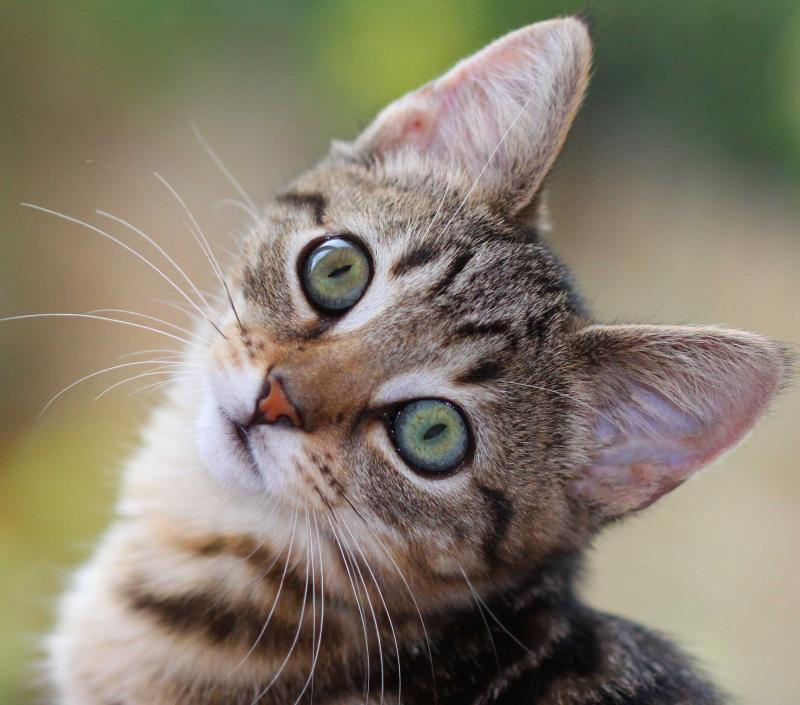
\includegraphics[width = 0.45\linewidth]{./images/kitten1}
	    \label{fig:cuteAnimals:kitten1}}
	\subfloat[golden tabby and white kitten]{\centering
	    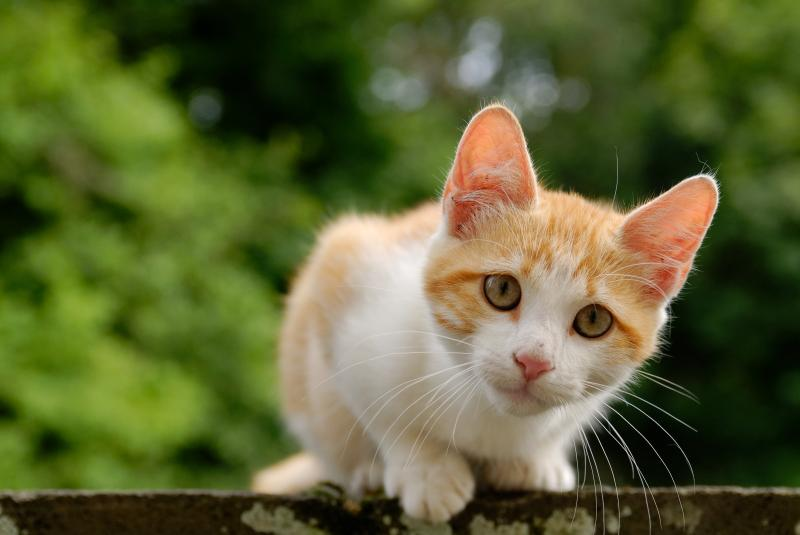
\includegraphics[width = 0.45\linewidth]{./images/kitten2}
	    \label{fig:cuteAnimals:kitten2}}\\[2em]
	\subfloat[Westie puppies]{\centering
	    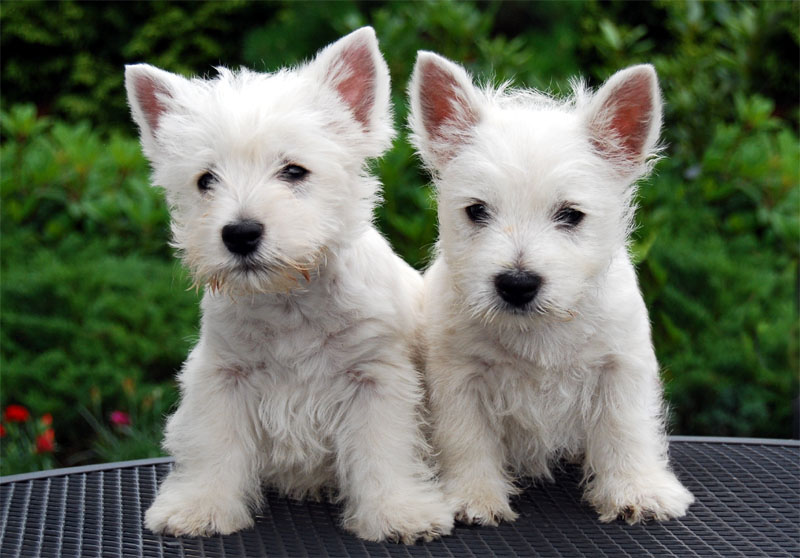
\includegraphics[width = 0.45\linewidth]{./images/puppy1}
	    \label{fig:cuteAnimals:puppy1}}
	\subfloat[St.\ Bernard puppy]{\centering
	    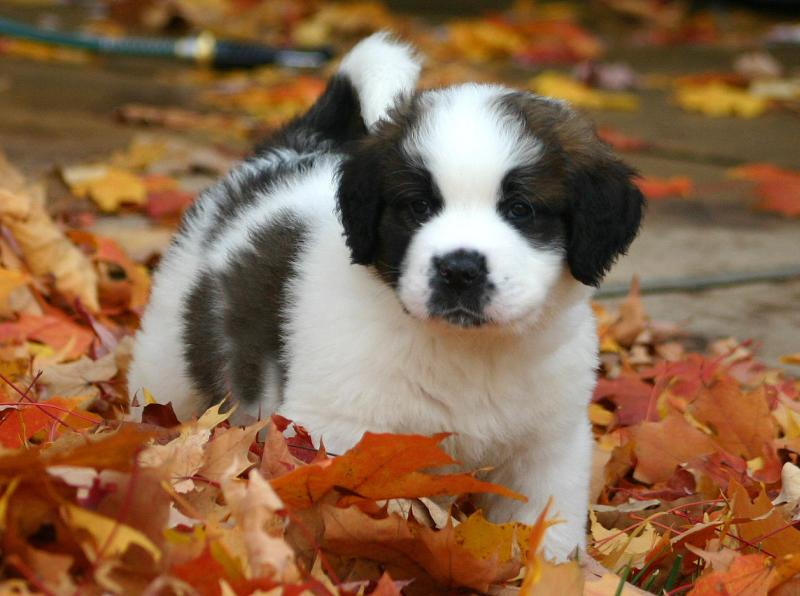
\includegraphics[width = 0.45\linewidth]{./images/puppy2}
	    \label{fig:cuteAnimals:puppy2}}
   \caption[Cute animals]{This is an example for subfigures and cute animals}
  \label{fig:cuteAnimals}
\end{figure}

\section{Tikz}

\subsection{Drawing with Tikz}

You can also add and resize TikZ figures, e.g.\ \cref{fig:tikzExample}.

\begin{figure}[p]
	\centering
	\resizebox{0.4\linewidth}{!}{\begin{tikzpicture}
    \foreach \i in {0,1,...,15} \draw[thick] (0.0, \i/7.5) -- +(-0.1, 0.1);
    \draw[thick] (0, 0) -- +(0, 2);

    \draw[tum green, -latex'] (2.0, 3) -- +(1, 0) node[midway, above] {$x$};
    \draw[tum green] (3, 1.8) -- +(0, 1.3);
    \draw[tum green] (2.0, 3) +(0, -0.2) -- +(0, 0.2);
    \foreach \i in {0,1,...,3} \draw[tum green] (2.0, 2.8 + \i/7.5) -- +(-0.1, 0.1);

    \def\dampY{0.60}
    \def\dampLX{0}
    \def\dampRX{3}
    \def\dampLRod{1.25}
    \def\dampRRod{1.2}
    \def\dampWPiston{0.14}
    \def\dampWCylinder{0.20}
    \def\dampLCylinder{0.6}

    \draw[thick] (\dampLX, \dampY) -- +(\dampLRod, 0); % Left rod to the piston
    \draw[thick] (\dampLX + \dampLRod, \dampY + \dampWPiston/2) -- +(0, -\dampWPiston); % Piston
    \draw[thick] (\dampRX - \dampRRod - \dampWCylinder/2, \dampY - \dampWCylinder/2) arc (-90:+90:\dampWCylinder/2); % Cylinder head
    \draw[thick] (\dampRX - \dampRRod - \dampWCylinder/2, \dampY + \dampWCylinder/2) -- +(-\dampLCylinder, 0);  % Upper cylinder
    \node[above] at (\dampRX - \dampRRod - \dampWCylinder/2 - \dampLCylinder/2, \dampY + \dampWCylinder/2) {$d$};
    \draw[thick] (\dampRX - \dampRRod - \dampWCylinder/2, \dampY - \dampWCylinder/2) -- +(-\dampLCylinder, 0); % Lower cylinder
    \draw[thick] (\dampRX, \dampY) -- +(-\dampRRod, 0); % Right rod to the cylinder head

    \def\springY{1.4}
    \def\springLX{0}
    \def\springRX{3}
    \def\springLRod{0.5}
    \def\springRRod{0.5}
    \def\springWCoil{0.20}
    \def\springNCoil{12}
    \pgfmathsetmacro{\springLCoil}{(\springRX - \springRRod - \springLX - \springLRod)/\springNCoil}

    \draw[thick] (\springLX, \springY) -- ++(\springLRod + 0.01, 0); % Left rod
    \draw[thick] (\springRX, \springY) -- ++(-\springRRod - 0.01, 0); % Right rod
    \foreach \i in {1, 2, ..., \springNCoil} %
        \draw[thick] (\springLX + \springLRod + \i*\springLCoil - \springLCoil, \springY) -- %
        ++(\springLCoil/4, -\springWCoil/2) -- ++(\springLCoil/2, +\springWCoil) -- ++(\springLCoil/4, -\springWCoil/2);
    \node[above] at ( \springLX/2 + \springLRod/2 + \springRX/2 - \springRRod/2, \springY + \springWCoil/2) {$c$};

    \draw[thick] (3, 0.2) rectangle +(2, 1.6) node[midway] {$m$};
\end{tikzpicture}
}
	\caption{Example for a TikZ figure}
	\label{fig:tikzExample}
\end{figure}

\begin{figure}[ht]
	\centering
	\begin{tikzpicture}

% Stützstellen
\draw [tum blue 3, fill]  (-3, -0.05) rectangle (-1, 0.05); 

\draw (-3, 0) node[below=0.6em] {$\underline{\mathbf{p}}_{i-1}$}  +(-0.2, 0.2)  -- +(0.2, -0.2);
\draw (-3, 0) node[above=0.6em] {$\underline{\mathbf{V}}_{i-1}$}  +(-0.2, -0.2)  -- +(0.2, 0.2);

\draw (-1, 0) node[below=0.6em] {$\overline{\mathbf{p}}_{i-1}$}  +(-0.2, 0.2)  -- +(0.2, -0.2);
\draw (-1, 0) node[above=0.6em] {$\overline{\mathbf{V}}_{i-1}$}  +(-0.2, -0.2)  -- +(0.2, 0.2);

%-------------------------------------------------------------------------------------------------
\draw [tum blue 2, fill]  (1, -0.05) rectangle (3, 0.05); 

\draw (1, 0) node[below=0.6em] {$\underline{\mathbf{p}}_{i}$}  +(-0.2, 0.2)  -- +(0.2, -0.2);
\draw (1, 0) node[above=0.6em] {$\underline{\mathbf{V}}_{i}$}  +(-0.2, -0.2)  -- +(0.2, 0.2);

\draw (3, 0) node[below=0.6em] {$\overline{\mathbf{p}}_{i}$}   +(-0.2, 0.2)  -- +(0.2, -0.2);
\draw (3, 0) node[above=0.6em] {$\overline{\mathbf{V}}_{i}$}  +(-0.2, -0.2)  -- +(0.2, 0.2);

% x-Achse
\draw[-latex'] (-4, 0) -- (4, 0) node[below] {$\mathbf{p}$};

% V_{t-1}
\draw[tum blue 4] (-2, 0) node[below=0.1em] {$\mathbf{p}_{t-1}$};
\draw[tum blue 4, thick, latex'-] (-2,0) +(0, 0) -- +(0, 2) node[above] {$\mathbf{V}_{t-1}$}; 

% V_{t}
\draw[tum blue 3] (2, 0) node[below=0.1em] {$\mathbf{p}_t$}; 
\draw[tum blue 3, thick, latex'-] (2,0) +(0, 0) -- +(0, 2) node[above] {$\mathbf{V}_{t}$}; 

% Dashed line
\draw[dashed,->] (-2, 1.5) -- (2, 1.5);

\end{tikzpicture}
	\caption{Illustration der verschiedenen Parameterstuetzstellen und deren lokalen Basen}
	\label{fig:ableitung_V}
\end{figure} 

\begin{figure}[hbp]
	\centering
	\begin{tikzpicture}
	 \node[anchor=south west,inner sep=0] (image) at (0,0) {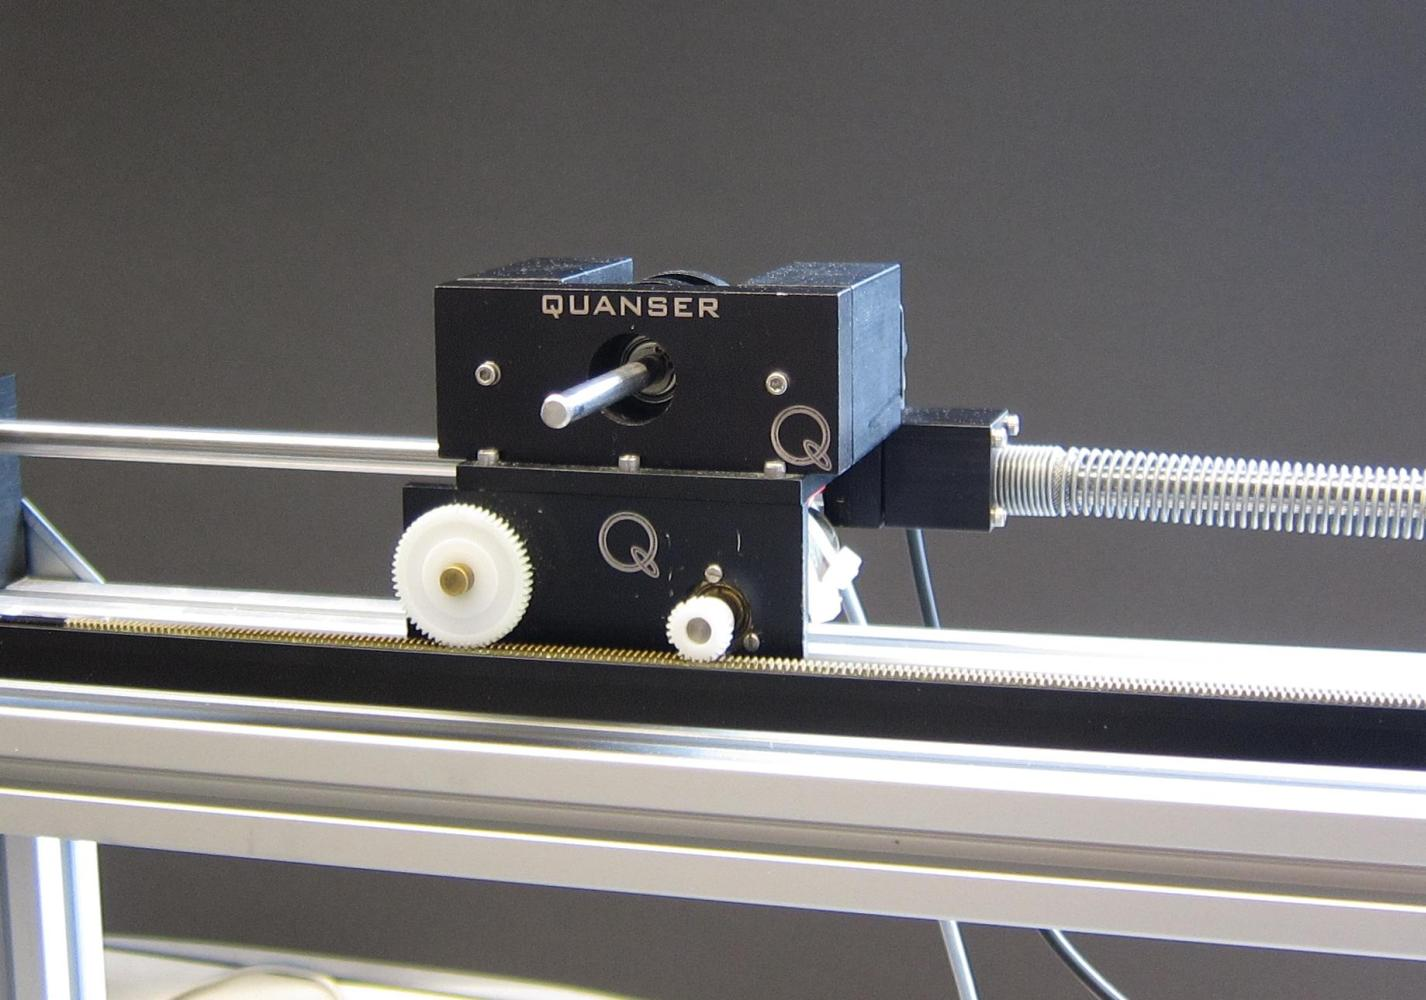
\includegraphics[width = 10 cm]{./images/wagen}};
	    \begin{scope}[x={(image.south east)},y={(image.north west)}]
	        \draw[white, thick, latex'-] (0.63, 0.74) -- +(0.1, 0.1) node[right] {Wagen};
	        \draw[white, thick, latex'-] (0.25, 0.58) -- +(-0.05, 0.1) node[left] {Schiene};
	        \draw[white, thick, latex'-] (0.32, 0.42) -- +(-0.05, -0.15) node[left, fill=black] {Sensorrad};
	        \draw[white, thick, latex'-] (0.49, 0.37) -- +(0.05, -0.15) node[right, fill=black] {Antriebsrad};
	    \end{scope}
\end{tikzpicture}
	\caption{Wagen in der Schienenfuehrung}
	\label{fig:aufbau:wagen}
\end{figure}

\begin{figure}
	\centering
	\begin{minipage}[c]{\textwidth}
		\centering
		%cwt-a
\begin{tikzpicture}[domain=0:3, scale=0.48]
\centering
		%KoordinatenSystem
		\draw[->] (0,0) -- (17,0) node[right]{$t$};
		\draw[->] (0,0) -- (0,17) node[left]{$a$};
		
		%-Rand vom Kasten
		\draw[] (16,0) -- (16,16);
		\draw[] (0,16) -- (16,16);
		
		%waagrechte Striche
		\draw[] (0,15) -- (16,15);
		\draw[] (0,14) -- (16,14);
		
		\draw[] (0,12) -- (16,12);

		\draw[] (0,8) -- (16,8);
		
		%senkrechte Striche		
		\draw[] (2,0) -- (2,8);
		\draw[] (4,0) -- (4,12);
		\draw[] (6,0) -- (6,8);
		\draw[] (8,0) -- (8,14);
		\draw[] (10,0) -- (10,8);
		\draw[] (12,0) -- (12,12);
		\draw[] (14,0) -- (14,8);			
\end{tikzpicture}




	
		\caption{Zeit-Skalierungsebene bei der Wavelet-Transformation}
		\label{fig:cwt_a}
	\end{minipage}\\[1em]
	\begin{minipage}[c]{\textwidth}
		\centering
		%cwt-f
\begin{tikzpicture}[domain=0:3, scale=0.48]
\centering
		%KoordinatenSystem
		\draw[->] (0,0) -- (17,0) node[right]{$t$};
		\draw[->] (0,0) -- (0,17) node[left]{$f$};
		
		%-Rand vom Kasten
		\draw[] (16,0) -- (16,16);
		\draw[] (0,16) -- (16,16);
		
		%waagrechte Striche
		\draw[] (0,1) -- (16,1);
		\draw[] (0,2) -- (16,2);
		\draw[] (0,4) -- (16,4);
		\draw[] (0,8) -- (16,8);
		\draw[] (0,16) -- (16,16);
		
		%senkrechte Striche		
		\draw[] (2,16) -- (2,8);
		\draw[] (4,16) -- (4,4);
		\draw[] (6,16) -- (6,8);
		\draw[] (8,16) -- (8,2);
		\draw[] (10,16) -- (10,8);
		\draw[] (12,16) -- (12,4);
		\draw[] (14,16) -- (14,8);
		
\end{tikzpicture}
		\caption{Zeit-Frequenzebene bei der Wavelet-Transformation}
		\label{fig:cwt_f}
	\end{minipage}
\end{figure}

%===================================================
\subsection{Matlab2Tikz}
You can download matlab2tikz from \url{https://de.mathworks.com/matlabcentral/fileexchange/22022-matlab2tikz-matlab2tikz}. It is nice because your plots are then drawn directly in \LaTeX{}. At the same time, if you have a lot of data, it can break your \TeX{} document or significantly increase the compilation time. Therefore, it is common practice to export figures (from MATLAB or anywhere else) as a PDF with a DPI of around 600, which you can then embed in your \TeX{} document

\begin{figure}[t!]
	\centering
	\begin{minipage}{0.95\linewidth}
		\centering
		\setlength\figureheight{3.3cm}
		\setlength\figurewidth{0.88\textwidth}
		% This file was created by matlab2tikz v0.4.6 running on MATLAB 7.13.
% Copyright (c) 2008--2014, Nico Schlömer <nico.schloemer@gmail.com>
% All rights reserved.
% Minimal pgfplots version: 1.3
% 
% The latest updates can be retrieved from
%   http://www.mathworks.com/matlabcentral/fileexchange/22022-matlab2tikz
% where you can also make suggestions and rate matlab2tikz.
% 
\begin{tikzpicture}

\begin{axis}[%
width=\figurewidth,
height=\figureheight,
scale only axis,
xmin=0,
xmax=20,
xlabel={Zeit $t$ / s},
ymin=-2.5,
ymax=2.5,
ylabel={$T_{\text{anr}}(t) \text{/Nm}$},
title={PRBS-Signal}
]
\addplot [color=blue,solid,line width=0.8pt,forget plot]
  table[row sep=crcr]{
0	-2.0019550342131	\\
0.02	-2.0019550342131	\\
0.04	-2.0019550342131	\\
0.06	-2.0019550342131	\\
0.08	-2.0019550342131	\\
0.1	-2.0019550342131	\\
0.12	-2.0019550342131	\\
0.14	-2.0019550342131	\\
0.16	-2.0019550342131	\\
0.18	-2.0019550342131	\\
0.2	-2.0019550342131	\\
0.22	-2.0019550342131	\\
0.24	-2.0019550342131	\\
0.26	-2.0019550342131	\\
0.28	-2.0019550342131	\\
0.3	-2.0019550342131	\\
0.32	-2.0019550342131	\\
0.34	-2.0019550342131	\\
0.36	-2.0019550342131	\\
0.38	-2.0019550342131	\\
0.4	1.9980449657869	\\
0.42	1.9980449657869	\\
0.44	-2.0019550342131	\\
0.46	-2.0019550342131	\\
0.48	-2.0019550342131	\\
0.5	-2.0019550342131	\\
0.52	-2.0019550342131	\\
0.54	-2.0019550342131	\\
0.56	-2.0019550342131	\\
0.58	-2.0019550342131	\\
0.6	-2.0019550342131	\\
0.62	-2.0019550342131	\\
0.64	-2.0019550342131	\\
0.66	-2.0019550342131	\\
0.68	1.9980449657869	\\
0.7	1.9980449657869	\\
0.72	-2.0019550342131	\\
0.74	-2.0019550342131	\\
0.76	-2.0019550342131	\\
0.78	-2.0019550342131	\\
0.8	1.9980449657869	\\
0.82	1.9980449657869	\\
0.84	-2.0019550342131	\\
0.86	-2.0019550342131	\\
0.88	-2.0019550342131	\\
0.9	-2.0019550342131	\\
0.92	-2.0019550342131	\\
0.94	-2.0019550342131	\\
0.96	1.9980449657869	\\
0.98	1.9980449657869	\\
1	-2.0019550342131	\\
1.02	-2.0019550342131	\\
1.04	-2.0019550342131	\\
1.06	-2.0019550342131	\\
1.08	-2.0019550342131	\\
1.1	-2.0019550342131	\\
1.12	-2.0019550342131	\\
1.14	-2.0019550342131	\\
1.16	-2.0019550342131	\\
1.18	-2.0019550342131	\\
1.2	1.9980449657869	\\
1.22	1.9980449657869	\\
1.24	1.9980449657869	\\
1.26	1.9980449657869	\\
1.28	-2.0019550342131	\\
1.3	-2.0019550342131	\\
1.32	-2.0019550342131	\\
1.34	-2.0019550342131	\\
1.36	1.9980449657869	\\
1.38	1.9980449657869	\\
1.4	-2.0019550342131	\\
1.42	-2.0019550342131	\\
1.44	-2.0019550342131	\\
1.46	-2.0019550342131	\\
1.48	1.9980449657869	\\
1.5	1.9980449657869	\\
1.52	1.9980449657869	\\
1.54	1.9980449657869	\\
1.56	-2.0019550342131	\\
1.58	-2.0019550342131	\\
1.6	1.9980449657869	\\
1.62	1.9980449657869	\\
1.64	-2.0019550342131	\\
1.66	-2.0019550342131	\\
1.68	-2.0019550342131	\\
1.7	-2.0019550342131	\\
1.72	-2.0019550342131	\\
1.74	-2.0019550342131	\\
1.76	-2.0019550342131	\\
1.78	-2.0019550342131	\\
1.8	1.9980449657869	\\
1.82	1.9980449657869	\\
1.84	-2.0019550342131	\\
1.86	-2.0019550342131	\\
1.88	-2.0019550342131	\\
1.9	-2.0019550342131	\\
1.92	1.9980449657869	\\
1.94	1.9980449657869	\\
1.96	-2.0019550342131	\\
1.98	-2.0019550342131	\\
2	1.9980449657869	\\
2.02	1.9980449657869	\\
2.04	-2.0019550342131	\\
2.06	-2.0019550342131	\\
2.08	1.9980449657869	\\
2.1	1.9980449657869	\\
2.12	-2.0019550342131	\\
2.14	-2.0019550342131	\\
2.16	-2.0019550342131	\\
2.18	-2.0019550342131	\\
2.2	-2.0019550342131	\\
2.22	-2.0019550342131	\\
2.24	-2.0019550342131	\\
2.26	-2.0019550342131	\\
2.28	1.9980449657869	\\
2.3	1.9980449657869	\\
2.32	1.9980449657869	\\
2.34	1.9980449657869	\\
2.36	1.9980449657869	\\
2.38	1.9980449657869	\\
2.4	1.9980449657869	\\
2.42	1.9980449657869	\\
2.44	-2.0019550342131	\\
2.46	-2.0019550342131	\\
2.48	1.9980449657869	\\
2.5	1.9980449657869	\\
2.52	-2.0019550342131	\\
2.54	-2.0019550342131	\\
2.56	1.9980449657869	\\
2.58	1.9980449657869	\\
2.6	1.9980449657869	\\
2.62	1.9980449657869	\\
2.64	1.9980449657869	\\
2.66	1.9980449657869	\\
2.68	-2.0019550342131	\\
2.7	-2.0019550342131	\\
2.72	1.9980449657869	\\
2.74	1.9980449657869	\\
2.76	-2.0019550342131	\\
2.78	-2.0019550342131	\\
2.8	1.9980449657869	\\
2.82	1.9980449657869	\\
2.84	1.9980449657869	\\
2.86	1.9980449657869	\\
2.88	-2.0019550342131	\\
2.9	-2.0019550342131	\\
2.92	1.9980449657869	\\
2.94	1.9980449657869	\\
2.96	1.9980449657869	\\
2.98	1.9980449657869	\\
3	-2.0019550342131	\\
3.02	-2.0019550342131	\\
3.04	1.9980449657869	\\
3.06	1.9980449657869	\\
3.08	1.9980449657869	\\
3.1	1.9980449657869	\\
3.12	-2.0019550342131	\\
3.14	-2.0019550342131	\\
3.16	-2.0019550342131	\\
3.18	-2.0019550342131	\\
3.2	-2.0019550342131	\\
3.22	-2.0019550342131	\\
3.24	-2.0019550342131	\\
3.26	-2.0019550342131	\\
3.28	-2.0019550342131	\\
3.3	-2.0019550342131	\\
3.32	-2.0019550342131	\\
3.34	-2.0019550342131	\\
3.36	-2.0019550342131	\\
3.38	-2.0019550342131	\\
3.4	-2.0019550342131	\\
3.42	-2.0019550342131	\\
3.44	1.9980449657869	\\
3.46	1.9980449657869	\\
3.48	1.9980449657869	\\
3.5	1.9980449657869	\\
3.52	-2.0019550342131	\\
3.54	-2.0019550342131	\\
3.56	-2.0019550342131	\\
3.58	-2.0019550342131	\\
3.6	-2.0019550342131	\\
3.62	-2.0019550342131	\\
3.64	-2.0019550342131	\\
3.66	-2.0019550342131	\\
3.68	-2.0019550342131	\\
3.7	-2.0019550342131	\\
3.72	1.9980449657869	\\
3.74	1.9980449657869	\\
3.76	1.9980449657869	\\
3.78	1.9980449657869	\\
3.8	-2.0019550342131	\\
3.82	-2.0019550342131	\\
3.84	1.9980449657869	\\
3.86	1.9980449657869	\\
3.88	1.9980449657869	\\
3.9	1.9980449657869	\\
3.92	-2.0019550342131	\\
3.94	-2.0019550342131	\\
3.96	-2.0019550342131	\\
3.98	-2.0019550342131	\\
4	1.9980449657869	\\
4.02	1.9980449657869	\\
4.04	1.9980449657869	\\
4.06	1.9980449657869	\\
4.08	-2.0019550342131	\\
4.1	-2.0019550342131	\\
4.12	-2.0019550342131	\\
4.14	-2.0019550342131	\\
4.16	-2.0019550342131	\\
4.18	-2.0019550342131	\\
4.2	-2.0019550342131	\\
4.22	-2.0019550342131	\\
4.24	1.9980449657869	\\
4.26	1.9980449657869	\\
4.28	-2.0019550342131	\\
4.3	-2.0019550342131	\\
4.32	1.9980449657869	\\
4.34	1.9980449657869	\\
4.36	-2.0019550342131	\\
4.38	-2.0019550342131	\\
4.4	1.9980449657869	\\
4.42	1.9980449657869	\\
4.44	1.9980449657869	\\
4.46	1.9980449657869	\\
4.48	-2.0019550342131	\\
4.5	-2.0019550342131	\\
4.52	1.9980449657869	\\
4.54	1.9980449657869	\\
4.56	-2.0019550342131	\\
4.58	-2.0019550342131	\\
4.6	1.9980449657869	\\
4.62	1.9980449657869	\\
4.64	1.9980449657869	\\
4.66	1.9980449657869	\\
4.68	1.9980449657869	\\
4.7	1.9980449657869	\\
4.72	-2.0019550342131	\\
4.74	-2.0019550342131	\\
4.76	-2.0019550342131	\\
4.78	-2.0019550342131	\\
4.8	-2.0019550342131	\\
4.82	-2.0019550342131	\\
4.84	1.9980449657869	\\
4.86	1.9980449657869	\\
4.88	1.9980449657869	\\
4.9	1.9980449657869	\\
4.92	-2.0019550342131	\\
4.94	-2.0019550342131	\\
4.96	1.9980449657869	\\
4.98	1.9980449657869	\\
5	1.9980449657869	\\
5.02	1.9980449657869	\\
5.04	1.9980449657869	\\
5.06	1.9980449657869	\\
5.08	1.9980449657869	\\
5.1	1.9980449657869	\\
5.12	1.9980449657869	\\
5.14	1.9980449657869	\\
5.16	1.9980449657869	\\
5.18	1.9980449657869	\\
5.2	-2.0019550342131	\\
5.22	-2.0019550342131	\\
5.24	-2.0019550342131	\\
5.26	-2.0019550342131	\\
5.28	-2.0019550342131	\\
5.3	-2.0019550342131	\\
5.32	1.9980449657869	\\
5.34	1.9980449657869	\\
5.36	-2.0019550342131	\\
5.38	-2.0019550342131	\\
5.4	-2.0019550342131	\\
5.42	-2.0019550342131	\\
5.44	-2.0019550342131	\\
5.46	-2.0019550342131	\\
5.48	1.9980449657869	\\
5.5	1.9980449657869	\\
5.52	1.9980449657869	\\
5.54	1.9980449657869	\\
5.56	1.9980449657869	\\
5.58	1.9980449657869	\\
5.6	1.9980449657869	\\
5.62	1.9980449657869	\\
5.64	-2.0019550342131	\\
5.66	-2.0019550342131	\\
5.68	-2.0019550342131	\\
5.7	-2.0019550342131	\\
5.72	1.9980449657869	\\
5.74	1.9980449657869	\\
5.76	1.9980449657869	\\
5.78	1.9980449657869	\\
5.8	1.9980449657869	\\
5.82	1.9980449657869	\\
5.84	1.9980449657869	\\
5.86	1.9980449657869	\\
5.88	-2.0019550342131	\\
5.9	-2.0019550342131	\\
5.92	1.9980449657869	\\
5.94	1.9980449657869	\\
5.96	1.9980449657869	\\
5.98	1.9980449657869	\\
6	-2.0019550342131	\\
6.02	-2.0019550342131	\\
6.04	1.9980449657869	\\
6.06	1.9980449657869	\\
6.08	1.9980449657869	\\
6.1	1.9980449657869	\\
6.12	-2.0019550342131	\\
6.14	-2.0019550342131	\\
6.16	1.9980449657869	\\
6.18	1.9980449657869	\\
6.2	-2.0019550342131	\\
6.22	-2.0019550342131	\\
6.24	-2.0019550342131	\\
6.26	-2.0019550342131	\\
6.28	-2.0019550342131	\\
6.3	-2.0019550342131	\\
6.32	-2.0019550342131	\\
6.34	-2.0019550342131	\\
6.36	-2.0019550342131	\\
6.38	-2.0019550342131	\\
6.4	-2.0019550342131	\\
6.42	-2.0019550342131	\\
6.44	-2.0019550342131	\\
6.46	-2.0019550342131	\\
6.48	1.9980449657869	\\
6.5	1.9980449657869	\\
6.52	-2.0019550342131	\\
6.54	-2.0019550342131	\\
6.56	1.9980449657869	\\
6.58	1.9980449657869	\\
6.6	-2.0019550342131	\\
6.62	-2.0019550342131	\\
6.64	-2.0019550342131	\\
6.66	-2.0019550342131	\\
6.68	-2.0019550342131	\\
6.7	-2.0019550342131	\\
6.72	-2.0019550342131	\\
6.74	-2.0019550342131	\\
6.76	1.9980449657869	\\
6.78	1.9980449657869	\\
6.8	-2.0019550342131	\\
6.82	-2.0019550342131	\\
6.84	1.9980449657869	\\
6.86	1.9980449657869	\\
6.88	1.9980449657869	\\
6.9	1.9980449657869	\\
6.92	-2.0019550342131	\\
6.94	-2.0019550342131	\\
6.96	1.9980449657869	\\
6.98	1.9980449657869	\\
7	-2.0019550342131	\\
7.02	-2.0019550342131	\\
7.04	1.9980449657869	\\
7.06	1.9980449657869	\\
7.08	-2.0019550342131	\\
7.1	-2.0019550342131	\\
7.12	1.9980449657869	\\
7.14	1.9980449657869	\\
7.16	-2.0019550342131	\\
7.18	-2.0019550342131	\\
7.2	-2.0019550342131	\\
7.22	-2.0019550342131	\\
7.24	-2.0019550342131	\\
7.26	-2.0019550342131	\\
7.28	1.9980449657869	\\
7.3	1.9980449657869	\\
7.32	1.9980449657869	\\
7.34	1.9980449657869	\\
7.36	1.9980449657869	\\
7.38	1.9980449657869	\\
7.4	1.9980449657869	\\
7.42	1.9980449657869	\\
7.44	1.9980449657869	\\
7.46	1.9980449657869	\\
7.48	-2.0019550342131	\\
7.5	-2.0019550342131	\\
7.52	1.9980449657869	\\
7.54	1.9980449657869	\\
7.56	1.9980449657869	\\
7.58	1.9980449657869	\\
7.6	1.9980449657869	\\
7.62	1.9980449657869	\\
7.64	1.9980449657869	\\
7.66	1.9980449657869	\\
7.68	-2.0019550342131	\\
7.7	-2.0019550342131	\\
7.72	-2.0019550342131	\\
7.74	-2.0019550342131	\\
7.76	1.9980449657869	\\
7.78	1.9980449657869	\\
7.8	-2.0019550342131	\\
7.82	-2.0019550342131	\\
7.84	-2.0019550342131	\\
7.86	-2.0019550342131	\\
7.88	1.9980449657869	\\
7.9	1.9980449657869	\\
7.92	-2.0019550342131	\\
7.94	-2.0019550342131	\\
7.96	1.9980449657869	\\
7.98	1.9980449657869	\\
8	1.9980449657869	\\
8.02	1.9980449657869	\\
8.04	-2.0019550342131	\\
8.06	-2.0019550342131	\\
8.08	-2.0019550342131	\\
8.1	-2.0019550342131	\\
8.12	-2.0019550342131	\\
8.14	-2.0019550342131	\\
8.16	-2.0019550342131	\\
8.18	-2.0019550342131	\\
8.2	-2.0019550342131	\\
8.22	-2.0019550342131	\\
8.24	1.9980449657869	\\
8.26	1.9980449657869	\\
8.28	-2.0019550342131	\\
8.3	-2.0019550342131	\\
8.32	-2.0019550342131	\\
8.34	-2.0019550342131	\\
8.36	1.9980449657869	\\
8.38	1.9980449657869	\\
8.4	1.9980449657869	\\
8.42	1.9980449657869	\\
8.44	-2.0019550342131	\\
8.46	-2.0019550342131	\\
8.48	-2.0019550342131	\\
8.5	-2.0019550342131	\\
8.52	1.9980449657869	\\
8.54	1.9980449657869	\\
8.56	-2.0019550342131	\\
8.58	-2.0019550342131	\\
8.6	-2.0019550342131	\\
8.62	-2.0019550342131	\\
8.64	-2.0019550342131	\\
8.66	-2.0019550342131	\\
8.68	1.9980449657869	\\
8.7	1.9980449657869	\\
8.72	-2.0019550342131	\\
8.74	-2.0019550342131	\\
8.76	1.9980449657869	\\
8.78	1.9980449657869	\\
8.8	-2.0019550342131	\\
8.82	-2.0019550342131	\\
8.84	-2.0019550342131	\\
8.86	-2.0019550342131	\\
8.88	-2.0019550342131	\\
8.9	-2.0019550342131	\\
8.92	1.9980449657869	\\
8.94	1.9980449657869	\\
8.96	1.9980449657869	\\
8.98	1.9980449657869	\\
9	-2.0019550342131	\\
9.02	-2.0019550342131	\\
9.04	1.9980449657869	\\
9.06	1.9980449657869	\\
9.08	1.9980449657869	\\
9.1	1.9980449657869	\\
9.12	-2.0019550342131	\\
9.14	-2.0019550342131	\\
9.16	1.9980449657869	\\
9.18	1.9980449657869	\\
9.2	1.9980449657869	\\
9.22	1.9980449657869	\\
9.24	1.9980449657869	\\
9.26	1.9980449657869	\\
9.28	-2.0019550342131	\\
9.3	-2.0019550342131	\\
9.32	-2.0019550342131	\\
9.34	-2.0019550342131	\\
9.36	-2.0019550342131	\\
9.38	-2.0019550342131	\\
9.4	-2.0019550342131	\\
9.42	-2.0019550342131	\\
9.44	-2.0019550342131	\\
9.46	-2.0019550342131	\\
9.48	-2.0019550342131	\\
9.5	-2.0019550342131	\\
9.52	1.9980449657869	\\
9.54	1.9980449657869	\\
9.56	1.9980449657869	\\
9.58	1.9980449657869	\\
9.6	1.9980449657869	\\
9.62	1.9980449657869	\\
9.64	1.9980449657869	\\
9.66	1.9980449657869	\\
9.68	-2.0019550342131	\\
9.7	-2.0019550342131	\\
9.72	-2.0019550342131	\\
9.74	-2.0019550342131	\\
9.76	-2.0019550342131	\\
9.78	-2.0019550342131	\\
9.8	1.9980449657869	\\
9.82	1.9980449657869	\\
9.84	1.9980449657869	\\
9.86	1.9980449657869	\\
9.88	1.9980449657869	\\
9.9	1.9980449657869	\\
9.92	-2.0019550342131	\\
9.94	-2.0019550342131	\\
9.96	1.9980449657869	\\
9.98	1.9980449657869	\\
10	1.9980449657869	\\
10.02	1.9980449657869	\\
10.04	1.9980449657869	\\
10.06	1.9980449657869	\\
10.08	1.9980449657869	\\
10.1	1.9980449657869	\\
10.12	1.9980449657869	\\
10.14	1.9980449657869	\\
10.16	1.9980449657869	\\
10.18	1.9980449657869	\\
10.2	1.9980449657869	\\
10.22	1.9980449657869	\\
10.24	-2.0019550342131	\\
10.26	-2.0019550342131	\\
10.28	-2.0019550342131	\\
10.3	-2.0019550342131	\\
10.32	1.9980449657869	\\
10.34	1.9980449657869	\\
10.36	-2.0019550342131	\\
10.38	-2.0019550342131	\\
10.4	-2.0019550342131	\\
10.42	-2.0019550342131	\\
10.44	-2.0019550342131	\\
10.46	-2.0019550342131	\\
10.48	-2.0019550342131	\\
10.5	-2.0019550342131	\\
10.52	1.9980449657869	\\
10.54	1.9980449657869	\\
10.56	1.9980449657869	\\
10.58	1.9980449657869	\\
10.6	-2.0019550342131	\\
10.62	-2.0019550342131	\\
10.64	-2.0019550342131	\\
10.66	-2.0019550342131	\\
10.68	-2.0019550342131	\\
10.7	-2.0019550342131	\\
10.72	1.9980449657869	\\
10.74	1.9980449657869	\\
10.76	-2.0019550342131	\\
10.78	-2.0019550342131	\\
10.8	1.9980449657869	\\
10.82	1.9980449657869	\\
10.84	1.9980449657869	\\
10.86	1.9980449657869	\\
10.88	-2.0019550342131	\\
10.9	-2.0019550342131	\\
10.92	1.9980449657869	\\
10.94	1.9980449657869	\\
10.96	1.9980449657869	\\
10.98	1.9980449657869	\\
11	1.9980449657869	\\
11.02	1.9980449657869	\\
11.04	-2.0019550342131	\\
11.06	-2.0019550342131	\\
11.08	1.9980449657869	\\
11.1	1.9980449657869	\\
11.12	-2.0019550342131	\\
11.14	-2.0019550342131	\\
11.16	-2.0019550342131	\\
11.18	-2.0019550342131	\\
11.2	-2.0019550342131	\\
11.22	-2.0019550342131	\\
11.24	-2.0019550342131	\\
11.26	-2.0019550342131	\\
11.28	1.9980449657869	\\
11.3	1.9980449657869	\\
11.32	1.9980449657869	\\
11.34	1.9980449657869	\\
11.36	-2.0019550342131	\\
11.38	-2.0019550342131	\\
11.4	1.9980449657869	\\
11.42	1.9980449657869	\\
11.44	-2.0019550342131	\\
11.46	-2.0019550342131	\\
11.48	1.9980449657869	\\
11.5	1.9980449657869	\\
11.52	-2.0019550342131	\\
11.54	-2.0019550342131	\\
11.56	1.9980449657869	\\
11.58	1.9980449657869	\\
11.6	1.9980449657869	\\
11.62	1.9980449657869	\\
11.64	-2.0019550342131	\\
11.66	-2.0019550342131	\\
11.68	-2.0019550342131	\\
11.7	-2.0019550342131	\\
11.72	1.9980449657869	\\
11.74	1.9980449657869	\\
11.76	1.9980449657869	\\
11.78	1.9980449657869	\\
11.8	1.9980449657869	\\
11.82	1.9980449657869	\\
11.84	1.9980449657869	\\
11.86	1.9980449657869	\\
11.88	-2.0019550342131	\\
11.9	-2.0019550342131	\\
11.92	-2.0019550342131	\\
11.94	-2.0019550342131	\\
11.96	1.9980449657869	\\
11.98	1.9980449657869	\\
12	-2.0019550342131	\\
12.02	-2.0019550342131	\\
12.04	1.9980449657869	\\
12.06	1.9980449657869	\\
12.08	1.9980449657869	\\
12.1	1.9980449657869	\\
12.12	-2.0019550342131	\\
12.14	-2.0019550342131	\\
12.16	1.9980449657869	\\
12.18	1.9980449657869	\\
12.2	1.9980449657869	\\
12.22	1.9980449657869	\\
12.24	-2.0019550342131	\\
12.26	-2.0019550342131	\\
12.28	-2.0019550342131	\\
12.3	-2.0019550342131	\\
12.32	1.9980449657869	\\
12.34	1.9980449657869	\\
12.36	-2.0019550342131	\\
12.38	-2.0019550342131	\\
12.4	-2.0019550342131	\\
12.42	-2.0019550342131	\\
12.44	-2.0019550342131	\\
12.46	-2.0019550342131	\\
12.48	-2.0019550342131	\\
12.5	-2.0019550342131	\\
12.52	-2.0019550342131	\\
12.54	-2.0019550342131	\\
12.56	1.9980449657869	\\
12.58	1.9980449657869	\\
12.6	-2.0019550342131	\\
12.62	-2.0019550342131	\\
12.64	-2.0019550342131	\\
12.66	-2.0019550342131	\\
12.68	-2.0019550342131	\\
12.7	-2.0019550342131	\\
12.72	1.9980449657869	\\
12.74	1.9980449657869	\\
12.76	-2.0019550342131	\\
12.78	-2.0019550342131	\\
12.8	-2.0019550342131	\\
12.82	-2.0019550342131	\\
12.84	1.9980449657869	\\
12.86	1.9980449657869	\\
12.88	-2.0019550342131	\\
12.9	-2.0019550342131	\\
12.92	-2.0019550342131	\\
12.94	-2.0019550342131	\\
12.96	1.9980449657869	\\
12.98	1.9980449657869	\\
13	1.9980449657869	\\
13.02	1.9980449657869	\\
13.04	-2.0019550342131	\\
13.06	-2.0019550342131	\\
13.08	-2.0019550342131	\\
13.1	-2.0019550342131	\\
13.12	-2.0019550342131	\\
13.14	-2.0019550342131	\\
13.16	-2.0019550342131	\\
13.18	-2.0019550342131	\\
13.2	-2.0019550342131	\\
13.22	-2.0019550342131	\\
13.24	-2.0019550342131	\\
13.26	-2.0019550342131	\\
13.28	1.9980449657869	\\
13.3	1.9980449657869	\\
13.32	-2.0019550342131	\\
13.34	-2.0019550342131	\\
13.36	1.9980449657869	\\
13.38	1.9980449657869	\\
13.4	1.9980449657869	\\
13.42	1.9980449657869	\\
13.44	-2.0019550342131	\\
13.46	-2.0019550342131	\\
13.48	-2.0019550342131	\\
13.5	-2.0019550342131	\\
13.52	-2.0019550342131	\\
13.54	-2.0019550342131	\\
13.56	1.9980449657869	\\
13.58	1.9980449657869	\\
13.6	-2.0019550342131	\\
13.62	-2.0019550342131	\\
13.64	1.9980449657869	\\
13.66	1.9980449657869	\\
13.68	-2.0019550342131	\\
13.7	-2.0019550342131	\\
13.72	-2.0019550342131	\\
13.74	-2.0019550342131	\\
13.76	1.9980449657869	\\
13.78	1.9980449657869	\\
13.8	1.9980449657869	\\
13.82	1.9980449657869	\\
13.84	1.9980449657869	\\
13.86	1.9980449657869	\\
13.88	-2.0019550342131	\\
13.9	-2.0019550342131	\\
13.92	1.9980449657869	\\
13.94	1.9980449657869	\\
13.96	1.9980449657869	\\
13.98	1.9980449657869	\\
14	-2.0019550342131	\\
14.02	-2.0019550342131	\\
14.04	-2.0019550342131	\\
14.06	-2.0019550342131	\\
14.08	1.9980449657869	\\
14.1	1.9980449657869	\\
14.12	1.9980449657869	\\
14.14	1.9980449657869	\\
14.16	1.9980449657869	\\
14.18	1.9980449657869	\\
14.2	-2.0019550342131	\\
14.22	-2.0019550342131	\\
14.24	-2.0019550342131	\\
14.26	-2.0019550342131	\\
14.28	-2.0019550342131	\\
14.3	-2.0019550342131	\\
14.32	1.9980449657869	\\
14.34	1.9980449657869	\\
14.36	-2.0019550342131	\\
14.38	-2.0019550342131	\\
14.4	1.9980449657869	\\
14.42	1.9980449657869	\\
14.44	1.9980449657869	\\
14.46	1.9980449657869	\\
14.48	1.9980449657869	\\
14.5	1.9980449657869	\\
14.52	1.9980449657869	\\
14.54	1.9980449657869	\\
14.56	1.9980449657869	\\
14.58	1.9980449657869	\\
14.6	1.9980449657869	\\
14.62	1.9980449657869	\\
14.64	-2.0019550342131	\\
14.66	-2.0019550342131	\\
14.68	1.9980449657869	\\
14.7	1.9980449657869	\\
14.72	-2.0019550342131	\\
14.74	-2.0019550342131	\\
14.76	1.9980449657869	\\
14.78	1.9980449657869	\\
14.8	-2.0019550342131	\\
14.82	-2.0019550342131	\\
14.84	-2.0019550342131	\\
14.86	-2.0019550342131	\\
14.88	-2.0019550342131	\\
14.9	-2.0019550342131	\\
14.92	1.9980449657869	\\
14.94	1.9980449657869	\\
14.96	-2.0019550342131	\\
14.98	-2.0019550342131	\\
15	1.9980449657869	\\
15.02	1.9980449657869	\\
15.04	1.9980449657869	\\
15.06	1.9980449657869	\\
15.08	1.9980449657869	\\
15.1	1.9980449657869	\\
15.12	-2.0019550342131	\\
15.14	-2.0019550342131	\\
15.16	1.9980449657869	\\
15.18	1.9980449657869	\\
15.2	1.9980449657869	\\
15.22	1.9980449657869	\\
15.24	-2.0019550342131	\\
15.26	-2.0019550342131	\\
15.28	1.9980449657869	\\
15.3	1.9980449657869	\\
15.32	-2.0019550342131	\\
15.34	-2.0019550342131	\\
15.36	1.9980449657869	\\
15.38	1.9980449657869	\\
15.4	1.9980449657869	\\
15.42	1.9980449657869	\\
15.44	-2.0019550342131	\\
15.46	-2.0019550342131	\\
15.48	-2.0019550342131	\\
15.5	-2.0019550342131	\\
15.52	-2.0019550342131	\\
15.54	-2.0019550342131	\\
15.56	-2.0019550342131	\\
15.58	-2.0019550342131	\\
15.6	1.9980449657869	\\
15.62	1.9980449657869	\\
15.64	1.9980449657869	\\
15.66	1.9980449657869	\\
15.68	-2.0019550342131	\\
15.7	-2.0019550342131	\\
15.72	-2.0019550342131	\\
15.74	-2.0019550342131	\\
15.76	1.9980449657869	\\
15.78	1.9980449657869	\\
15.8	1.9980449657869	\\
15.82	1.9980449657869	\\
15.84	-2.0019550342131	\\
15.86	-2.0019550342131	\\
15.88	1.9980449657869	\\
15.9	1.9980449657869	\\
15.92	1.9980449657869	\\
15.94	1.9980449657869	\\
15.96	-2.0019550342131	\\
15.98	-2.0019550342131	\\
16	1.9980449657869	\\
16.02	1.9980449657869	\\
16.04	-2.0019550342131	\\
16.06	-2.0019550342131	\\
16.08	1.9980449657869	\\
16.1	1.9980449657869	\\
16.12	-2.0019550342131	\\
16.14	-2.0019550342131	\\
16.16	-2.0019550342131	\\
16.18	-2.0019550342131	\\
16.2	-2.0019550342131	\\
16.22	-2.0019550342131	\\
16.24	-2.0019550342131	\\
16.26	-2.0019550342131	\\
16.28	-2.0019550342131	\\
16.3	-2.0019550342131	\\
16.32	1.9980449657869	\\
16.34	1.9980449657869	\\
16.36	1.9980449657869	\\
16.38	1.9980449657869	\\
16.4	1.9980449657869	\\
16.42	1.9980449657869	\\
16.44	-2.0019550342131	\\
16.46	-2.0019550342131	\\
16.48	1.9980449657869	\\
16.5	1.9980449657869	\\
16.52	-2.0019550342131	\\
16.54	-2.0019550342131	\\
16.56	-2.0019550342131	\\
16.58	-2.0019550342131	\\
16.6	1.9980449657869	\\
16.62	1.9980449657869	\\
16.64	1.9980449657869	\\
16.66	1.9980449657869	\\
16.68	1.9980449657869	\\
16.7	1.9980449657869	\\
16.72	1.9980449657869	\\
16.74	1.9980449657869	\\
16.76	-2.0019550342131	\\
16.78	-2.0019550342131	\\
16.8	1.9980449657869	\\
16.82	1.9980449657869	\\
16.84	-2.0019550342131	\\
16.86	-2.0019550342131	\\
16.88	-2.0019550342131	\\
16.9	-2.0019550342131	\\
16.92	1.9980449657869	\\
16.94	1.9980449657869	\\
16.96	1.9980449657869	\\
16.98	1.9980449657869	\\
17	-2.0019550342131	\\
17.02	-2.0019550342131	\\
17.04	1.9980449657869	\\
17.06	1.9980449657869	\\
17.08	-2.0019550342131	\\
17.1	-2.0019550342131	\\
17.12	1.9980449657869	\\
17.14	1.9980449657869	\\
17.16	-2.0019550342131	\\
17.18	-2.0019550342131	\\
17.2	-2.0019550342131	\\
17.22	-2.0019550342131	\\
17.24	1.9980449657869	\\
17.26	1.9980449657869	\\
17.28	-2.0019550342131	\\
17.3	-2.0019550342131	\\
17.32	-2.0019550342131	\\
17.34	-2.0019550342131	\\
17.36	1.9980449657869	\\
17.38	1.9980449657869	\\
17.4	1.9980449657869	\\
17.42	1.9980449657869	\\
17.44	1.9980449657869	\\
17.46	1.9980449657869	\\
17.48	-2.0019550342131	\\
17.5	-2.0019550342131	\\
17.52	-2.0019550342131	\\
17.54	-2.0019550342131	\\
17.56	-2.0019550342131	\\
17.58	-2.0019550342131	\\
17.6	-2.0019550342131	\\
17.62	-2.0019550342131	\\
17.64	-2.0019550342131	\\
17.66	-2.0019550342131	\\
17.68	1.9980449657869	\\
17.7	1.9980449657869	\\
17.72	1.9980449657869	\\
17.74	1.9980449657869	\\
17.76	1.9980449657869	\\
17.78	1.9980449657869	\\
17.8	1.9980449657869	\\
17.82	1.9980449657869	\\
17.84	1.9980449657869	\\
17.86	1.9980449657869	\\
17.88	-2.0019550342131	\\
17.9	-2.0019550342131	\\
17.92	-2.0019550342131	\\
17.94	-2.0019550342131	\\
17.96	1.9980449657869	\\
17.98	1.9980449657869	\\
18	1.9980449657869	\\
18.02	1.9980449657869	\\
18.04	1.9980449657869	\\
18.06	1.9980449657869	\\
18.08	-2.0019550342131	\\
18.1	-2.0019550342131	\\
18.12	-2.0019550342131	\\
18.14	-2.0019550342131	\\
18.16	1.9980449657869	\\
18.18	1.9980449657869	\\
18.2	1.9980449657869	\\
18.22	1.9980449657869	\\
18.24	-2.0019550342131	\\
18.26	-2.0019550342131	\\
18.28	1.9980449657869	\\
18.3	1.9980449657869	\\
18.32	1.9980449657869	\\
18.34	1.9980449657869	\\
18.36	1.9980449657869	\\
18.38	1.9980449657869	\\
18.4	1.9980449657869	\\
18.42	1.9980449657869	\\
18.44	-2.0019550342131	\\
18.46	-2.0019550342131	\\
18.48	1.9980449657869	\\
18.5	1.9980449657869	\\
18.52	-2.0019550342131	\\
18.54	-2.0019550342131	\\
18.56	-2.0019550342131	\\
18.58	-2.0019550342131	\\
18.6	-2.0019550342131	\\
18.62	-2.0019550342131	\\
18.64	1.9980449657869	\\
18.66	1.9980449657869	\\
18.68	-2.0019550342131	\\
18.7	-2.0019550342131	\\
18.72	1.9980449657869	\\
18.74	1.9980449657869	\\
18.76	-2.0019550342131	\\
18.78	-2.0019550342131	\\
18.8	1.9980449657869	\\
18.82	1.9980449657869	\\
18.84	-2.0019550342131	\\
18.86	-2.0019550342131	\\
18.88	1.9980449657869	\\
18.9	1.9980449657869	\\
18.92	1.9980449657869	\\
18.94	1.9980449657869	\\
18.96	-2.0019550342131	\\
18.98	-2.0019550342131	\\
19	1.9980449657869	\\
19.02	1.9980449657869	\\
19.04	1.9980449657869	\\
19.06	1.9980449657869	\\
19.08	1.9980449657869	\\
19.1	1.9980449657869	\\
19.12	1.9980449657869	\\
19.14	1.9980449657869	\\
19.16	1.9980449657869	\\
19.18	1.9980449657869	\\
19.2	-2.0019550342131	\\
19.22	-2.0019550342131	\\
19.24	-2.0019550342131	\\
19.26	-2.0019550342131	\\
19.28	-2.0019550342131	\\
19.3	-2.0019550342131	\\
19.32	-2.0019550342131	\\
19.34	-2.0019550342131	\\
19.36	1.9980449657869	\\
19.38	1.9980449657869	\\
19.4	-2.0019550342131	\\
19.42	-2.0019550342131	\\
19.44	-2.0019550342131	\\
19.46	-2.0019550342131	\\
19.48	1.9980449657869	\\
19.5	1.9980449657869	\\
19.52	1.9980449657869	\\
19.54	1.9980449657869	\\
19.56	1.9980449657869	\\
19.58	1.9980449657869	\\
19.6	-2.0019550342131	\\
19.62	-2.0019550342131	\\
19.64	1.9980449657869	\\
19.66	1.9980449657869	\\
19.68	-2.0019550342131	\\
19.7	-2.0019550342131	\\
19.72	-2.0019550342131	\\
19.74	-2.0019550342131	\\
19.76	-2.0019550342131	\\
19.78	-2.0019550342131	\\
19.8	1.9980449657869	\\
19.82	1.9980449657869	\\
19.84	1.9980449657869	\\
19.86	1.9980449657869	\\
19.88	1.9980449657869	\\
19.9	1.9980449657869	\\
19.92	-2.0019550342131	\\
19.94	-2.0019550342131	\\
19.96	1.9980449657869	\\
19.98	1.9980449657869	\\
20	-2.0019550342131	\\
20.02	-2.0019550342131	\\
20.04	1.9980449657869	\\
20.06	1.9980449657869	\\
20.08	1.9980449657869	\\
20.1	1.9980449657869	\\
20.12	1.9980449657869	\\
20.14	1.9980449657869	\\
20.16	1.9980449657869	\\
20.18	1.9980449657869	\\
20.2	1.9980449657869	\\
20.22	1.9980449657869	\\
20.24	-2.0019550342131	\\
20.26	-2.0019550342131	\\
20.28	1.9980449657869	\\
20.3	1.9980449657869	\\
20.32	1.9980449657869	\\
20.34	1.9980449657869	\\
20.36	-2.0019550342131	\\
20.38	-2.0019550342131	\\
20.4	1.9980449657869	\\
20.42	1.9980449657869	\\
20.44	-2.0019550342131	\\
20.46	-2.0019550342131	\\
20.48	-2.0019550342131	\\
20.5	-2.0019550342131	\\
20.52	1.9980449657869	\\
20.54	1.9980449657869	\\
20.56	-2.0019550342131	\\
20.58	-2.0019550342131	\\
20.6	-2.0019550342131	\\
20.62	-2.0019550342131	\\
20.64	-2.0019550342131	\\
20.66	-2.0019550342131	\\
20.68	-2.0019550342131	\\
20.7	-2.0019550342131	\\
20.72	1.9980449657869	\\
20.74	1.9980449657869	\\
20.76	-2.0019550342131	\\
20.78	-2.0019550342131	\\
20.8	-2.0019550342131	\\
20.82	-2.0019550342131	\\
20.84	-2.0019550342131	\\
20.86	-2.0019550342131	\\
20.88	-2.0019550342131	\\
20.9	-2.0019550342131	\\
20.92	1.9980449657869	\\
20.94	1.9980449657869	\\
20.96	-2.0019550342131	\\
20.98	-2.0019550342131	\\
21	1.9980449657869	\\
21.02	1.9980449657869	\\
21.04	-2.0019550342131	\\
21.06	-2.0019550342131	\\
21.08	-2.0019550342131	\\
21.1	-2.0019550342131	\\
21.12	1.9980449657869	\\
21.14	1.9980449657869	\\
21.16	-2.0019550342131	\\
21.18	-2.0019550342131	\\
21.2	1.9980449657869	\\
21.22	1.9980449657869	\\
21.24	-2.0019550342131	\\
21.26	-2.0019550342131	\\
21.28	1.9980449657869	\\
21.3	1.9980449657869	\\
21.32	1.9980449657869	\\
21.34	1.9980449657869	\\
21.36	-2.0019550342131	\\
21.38	-2.0019550342131	\\
21.4	-2.0019550342131	\\
21.42	-2.0019550342131	\\
21.44	-2.0019550342131	\\
21.46	-2.0019550342131	\\
21.48	1.9980449657869	\\
21.5	1.9980449657869	\\
21.52	1.9980449657869	\\
21.54	1.9980449657869	\\
21.56	1.9980449657869	\\
21.58	1.9980449657869	\\
21.6	-2.0019550342131	\\
21.62	-2.0019550342131	\\
21.64	-2.0019550342131	\\
21.66	-2.0019550342131	\\
21.68	1.9980449657869	\\
21.7	1.9980449657869	\\
21.72	1.9980449657869	\\
21.74	1.9980449657869	\\
21.76	1.9980449657869	\\
21.78	1.9980449657869	\\
21.8	1.9980449657869	\\
21.82	1.9980449657869	\\
21.84	1.9980449657869	\\
21.86	1.9980449657869	\\
21.88	1.9980449657869	\\
21.9	1.9980449657869	\\
21.92	1.9980449657869	\\
21.94	1.9980449657869	\\
21.96	-2.0019550342131	\\
21.98	-2.0019550342131	\\
22	1.9980449657869	\\
22.02	1.9980449657869	\\
22.04	1.9980449657869	\\
22.06	1.9980449657869	\\
22.08	-2.0019550342131	\\
22.1	-2.0019550342131	\\
22.12	-2.0019550342131	\\
22.14	-2.0019550342131	\\
22.16	-2.0019550342131	\\
22.18	-2.0019550342131	\\
22.2	-2.0019550342131	\\
22.22	-2.0019550342131	\\
22.24	1.9980449657869	\\
22.26	1.9980449657869	\\
22.28	-2.0019550342131	\\
22.3	-2.0019550342131	\\
22.32	-2.0019550342131	\\
22.34	-2.0019550342131	\\
22.36	-2.0019550342131	\\
22.38	-2.0019550342131	\\
22.4	1.9980449657869	\\
22.42	1.9980449657869	\\
22.44	1.9980449657869	\\
22.46	1.9980449657869	\\
22.48	-2.0019550342131	\\
22.5	-2.0019550342131	\\
22.52	1.9980449657869	\\
22.54	1.9980449657869	\\
22.56	-2.0019550342131	\\
22.58	-2.0019550342131	\\
22.6	-2.0019550342131	\\
22.62	-2.0019550342131	\\
22.64	1.9980449657869	\\
22.66	1.9980449657869	\\
22.68	1.9980449657869	\\
22.7	1.9980449657869	\\
22.72	1.9980449657869	\\
22.74	1.9980449657869	\\
22.76	-2.0019550342131	\\
22.78	-2.0019550342131	\\
22.8	-2.0019550342131	\\
22.82	-2.0019550342131	\\
22.84	1.9980449657869	\\
22.86	1.9980449657869	\\
22.88	-2.0019550342131	\\
22.9	-2.0019550342131	\\
22.92	-2.0019550342131	\\
22.94	-2.0019550342131	\\
22.96	1.9980449657869	\\
22.98	1.9980449657869	\\
23	1.9980449657869	\\
23.02	1.9980449657869	\\
23.04	1.9980449657869	\\
23.06	1.9980449657869	\\
23.08	1.9980449657869	\\
23.1	1.9980449657869	\\
23.12	-2.0019550342131	\\
23.14	-2.0019550342131	\\
23.16	-2.0019550342131	\\
23.18	-2.0019550342131	\\
23.2	-2.0019550342131	\\
23.22	-2.0019550342131	\\
23.24	-2.0019550342131	\\
23.26	-2.0019550342131	\\
23.28	1.9980449657869	\\
23.3	1.9980449657869	\\
23.32	1.9980449657869	\\
23.34	1.9980449657869	\\
23.36	-2.0019550342131	\\
23.38	-2.0019550342131	\\
23.4	1.9980449657869	\\
23.42	1.9980449657869	\\
23.44	1.9980449657869	\\
23.46	1.9980449657869	\\
23.48	1.9980449657869	\\
23.5	1.9980449657869	\\
23.52	-2.0019550342131	\\
23.54	-2.0019550342131	\\
23.56	1.9980449657869	\\
23.58	1.9980449657869	\\
23.6	1.9980449657869	\\
23.62	1.9980449657869	\\
23.64	-2.0019550342131	\\
23.66	-2.0019550342131	\\
23.68	-2.0019550342131	\\
23.7	-2.0019550342131	\\
23.72	-2.0019550342131	\\
23.74	-2.0019550342131	\\
23.76	1.9980449657869	\\
23.78	1.9980449657869	\\
23.8	1.9980449657869	\\
23.82	1.9980449657869	\\
23.84	-2.0019550342131	\\
23.86	-2.0019550342131	\\
23.88	-2.0019550342131	\\
23.9	-2.0019550342131	\\
23.92	-2.0019550342131	\\
23.94	-2.0019550342131	\\
23.96	1.9980449657869	\\
23.98	1.9980449657869	\\
24	1.9980449657869	\\
24.02	1.9980449657869	\\
24.04	1.9980449657869	\\
24.06	1.9980449657869	\\
24.08	1.9980449657869	\\
24.1	1.9980449657869	\\
24.12	-2.0019550342131	\\
24.14	-2.0019550342131	\\
24.16	1.9980449657869	\\
24.18	1.9980449657869	\\
24.2	1.9980449657869	\\
24.22	1.9980449657869	\\
24.24	1.9980449657869	\\
24.26	1.9980449657869	\\
24.28	1.9980449657869	\\
24.3	1.9980449657869	\\
24.32	1.9980449657869	\\
24.34	1.9980449657869	\\
24.36	-2.0019550342131	\\
24.38	-2.0019550342131	\\
24.4	1.9980449657869	\\
24.42	1.9980449657869	\\
24.44	-2.0019550342131	\\
24.46	-2.0019550342131	\\
24.48	-2.0019550342131	\\
24.5	-2.0019550342131	\\
24.52	1.9980449657869	\\
24.54	1.9980449657869	\\
24.56	-2.0019550342131	\\
24.58	-2.0019550342131	\\
24.6	-2.0019550342131	\\
24.62	-2.0019550342131	\\
24.64	1.9980449657869	\\
24.66	1.9980449657869	\\
24.68	-2.0019550342131	\\
24.7	-2.0019550342131	\\
24.72	1.9980449657869	\\
24.74	1.9980449657869	\\
24.76	-2.0019550342131	\\
24.78	-2.0019550342131	\\
24.8	-2.0019550342131	\\
24.82	-2.0019550342131	\\
24.84	-2.0019550342131	\\
24.86	-2.0019550342131	\\
24.88	-2.0019550342131	\\
24.9	-2.0019550342131	\\
24.92	-2.0019550342131	\\
24.94	-2.0019550342131	\\
24.96	-2.0019550342131	\\
24.98	-2.0019550342131	\\
25	1.9980449657869	\\
25.02	1.9980449657869	\\
25.04	1.9980449657869	\\
25.06	1.9980449657869	\\
25.08	-2.0019550342131	\\
25.1	-2.0019550342131	\\
25.12	1.9980449657869	\\
25.14	1.9980449657869	\\
25.16	-2.0019550342131	\\
25.18	-2.0019550342131	\\
25.2	-2.0019550342131	\\
25.22	-2.0019550342131	\\
25.24	-2.0019550342131	\\
25.26	-2.0019550342131	\\
25.28	1.9980449657869	\\
25.3	1.9980449657869	\\
25.32	1.9980449657869	\\
25.34	1.9980449657869	\\
25.36	-2.0019550342131	\\
25.38	-2.0019550342131	\\
25.4	-2.0019550342131	\\
25.42	-2.0019550342131	\\
25.44	1.9980449657869	\\
25.46	1.9980449657869	\\
25.48	-2.0019550342131	\\
25.5	-2.0019550342131	\\
25.52	1.9980449657869	\\
25.54	1.9980449657869	\\
25.56	1.9980449657869	\\
25.58	1.9980449657869	\\
25.6	1.9980449657869	\\
25.62	1.9980449657869	\\
25.64	-2.0019550342131	\\
25.66	-2.0019550342131	\\
25.68	1.9980449657869	\\
25.7	1.9980449657869	\\
25.72	-2.0019550342131	\\
25.74	-2.0019550342131	\\
25.76	-2.0019550342131	\\
25.78	-2.0019550342131	\\
25.8	1.9980449657869	\\
25.82	1.9980449657869	\\
25.84	-2.0019550342131	\\
25.86	-2.0019550342131	\\
25.88	1.9980449657869	\\
25.9	1.9980449657869	\\
25.92	1.9980449657869	\\
25.94	1.9980449657869	\\
25.96	-2.0019550342131	\\
25.98	-2.0019550342131	\\
26	1.9980449657869	\\
26.02	1.9980449657869	\\
26.04	-2.0019550342131	\\
26.06	-2.0019550342131	\\
26.08	-2.0019550342131	\\
26.1	-2.0019550342131	\\
26.12	-2.0019550342131	\\
26.14	-2.0019550342131	\\
26.16	1.9980449657869	\\
26.18	1.9980449657869	\\
26.2	-2.0019550342131	\\
26.22	-2.0019550342131	\\
26.24	-2.0019550342131	\\
26.26	-2.0019550342131	\\
26.28	-2.0019550342131	\\
26.3	-2.0019550342131	\\
26.32	1.9980449657869	\\
26.34	1.9980449657869	\\
26.36	-2.0019550342131	\\
26.38	-2.0019550342131	\\
26.4	1.9980449657869	\\
26.42	1.9980449657869	\\
26.44	1.9980449657869	\\
26.46	1.9980449657869	\\
26.48	-2.0019550342131	\\
26.5	-2.0019550342131	\\
26.52	-2.0019550342131	\\
26.54	-2.0019550342131	\\
26.56	1.9980449657869	\\
26.58	1.9980449657869	\\
26.6	1.9980449657869	\\
26.62	1.9980449657869	\\
26.64	-2.0019550342131	\\
26.66	-2.0019550342131	\\
26.68	1.9980449657869	\\
26.7	1.9980449657869	\\
26.72	-2.0019550342131	\\
26.74	-2.0019550342131	\\
26.76	-2.0019550342131	\\
26.78	-2.0019550342131	\\
26.8	1.9980449657869	\\
26.82	1.9980449657869	\\
26.84	-2.0019550342131	\\
26.86	-2.0019550342131	\\
26.88	1.9980449657869	\\
26.9	1.9980449657869	\\
26.92	-2.0019550342131	\\
26.94	-2.0019550342131	\\
26.96	-2.0019550342131	\\
26.98	-2.0019550342131	\\
27	1.9980449657869	\\
27.02	1.9980449657869	\\
27.04	-2.0019550342131	\\
27.06	-2.0019550342131	\\
27.08	-2.0019550342131	\\
27.1	-2.0019550342131	\\
27.12	-2.0019550342131	\\
27.14	-2.0019550342131	\\
27.16	1.9980449657869	\\
27.18	1.9980449657869	\\
27.2	1.9980449657869	\\
27.22	1.9980449657869	\\
27.24	-2.0019550342131	\\
27.26	-2.0019550342131	\\
27.28	-2.0019550342131	\\
27.3	-2.0019550342131	\\
27.32	-2.0019550342131	\\
27.34	-2.0019550342131	\\
27.36	-2.0019550342131	\\
27.38	-2.0019550342131	\\
27.4	1.9980449657869	\\
27.42	1.9980449657869	\\
27.44	1.9980449657869	\\
27.46	1.9980449657869	\\
27.48	1.9980449657869	\\
27.5	1.9980449657869	\\
27.52	-2.0019550342131	\\
27.54	-2.0019550342131	\\
27.56	1.9980449657869	\\
27.58	1.9980449657869	\\
27.6	1.9980449657869	\\
27.62	1.9980449657869	\\
27.64	-2.0019550342131	\\
27.66	-2.0019550342131	\\
27.68	1.9980449657869	\\
27.7	1.9980449657869	\\
27.72	1.9980449657869	\\
27.74	1.9980449657869	\\
27.76	1.9980449657869	\\
27.78	1.9980449657869	\\
27.8	1.9980449657869	\\
27.82	1.9980449657869	\\
27.84	-2.0019550342131	\\
27.86	-2.0019550342131	\\
27.88	-2.0019550342131	\\
27.9	-2.0019550342131	\\
27.92	-2.0019550342131	\\
27.94	-2.0019550342131	\\
27.96	-2.0019550342131	\\
27.98	-2.0019550342131	\\
28	-2.0019550342131	\\
28.02	-2.0019550342131	\\
28.04	1.9980449657869	\\
28.06	1.9980449657869	\\
28.08	-2.0019550342131	\\
28.1	-2.0019550342131	\\
28.12	1.9980449657869	\\
28.14	1.9980449657869	\\
28.16	1.9980449657869	\\
28.18	1.9980449657869	\\
28.2	1.9980449657869	\\
28.22	1.9980449657869	\\
28.24	-2.0019550342131	\\
28.26	-2.0019550342131	\\
28.28	-2.0019550342131	\\
28.3	-2.0019550342131	\\
28.32	1.9980449657869	\\
28.34	1.9980449657869	\\
28.36	-2.0019550342131	\\
28.38	-2.0019550342131	\\
28.4	1.9980449657869	\\
28.42	1.9980449657869	\\
28.44	-2.0019550342131	\\
28.46	-2.0019550342131	\\
28.48	1.9980449657869	\\
28.5	1.9980449657869	\\
28.52	1.9980449657869	\\
28.54	1.9980449657869	\\
28.56	1.9980449657869	\\
28.58	1.9980449657869	\\
28.6	-2.0019550342131	\\
28.62	-2.0019550342131	\\
28.64	-2.0019550342131	\\
28.66	-2.0019550342131	\\
28.68	1.9980449657869	\\
28.7	1.9980449657869	\\
28.72	1.9980449657869	\\
28.74	1.9980449657869	\\
28.76	1.9980449657869	\\
28.78	1.9980449657869	\\
28.8	-2.0019550342131	\\
28.82	-2.0019550342131	\\
28.84	1.9980449657869	\\
28.86	1.9980449657869	\\
28.88	1.9980449657869	\\
28.9	1.9980449657869	\\
28.92	1.9980449657869	\\
28.94	1.9980449657869	\\
28.96	-2.0019550342131	\\
28.98	-2.0019550342131	\\
29	1.9980449657869	\\
29.02	1.9980449657869	\\
29.04	1.9980449657869	\\
29.06	1.9980449657869	\\
29.08	1.9980449657869	\\
29.1	1.9980449657869	\\
29.12	-2.0019550342131	\\
29.14	-2.0019550342131	\\
29.16	-2.0019550342131	\\
29.18	-2.0019550342131	\\
29.2	1.9980449657869	\\
29.22	1.9980449657869	\\
29.24	1.9980449657869	\\
29.26	1.9980449657869	\\
29.28	-2.0019550342131	\\
29.3	-2.0019550342131	\\
29.32	-2.0019550342131	\\
29.34	-2.0019550342131	\\
29.36	1.9980449657869	\\
29.38	1.9980449657869	\\
29.4	1.9980449657869	\\
29.42	1.9980449657869	\\
29.44	1.9980449657869	\\
29.46	1.9980449657869	\\
29.48	-2.0019550342131	\\
29.5	-2.0019550342131	\\
29.52	1.9980449657869	\\
29.54	1.9980449657869	\\
29.56	-2.0019550342131	\\
29.58	-2.0019550342131	\\
29.6	1.9980449657869	\\
29.62	1.9980449657869	\\
29.64	-2.0019550342131	\\
29.66	-2.0019550342131	\\
29.68	1.9980449657869	\\
29.7	1.9980449657869	\\
29.72	1.9980449657869	\\
29.74	1.9980449657869	\\
29.76	1.9980449657869	\\
29.78	1.9980449657869	\\
29.8	-2.0019550342131	\\
29.82	-2.0019550342131	\\
29.84	1.9980449657869	\\
29.86	1.9980449657869	\\
29.88	1.9980449657869	\\
29.9	1.9980449657869	\\
29.92	1.9980449657869	\\
29.94	1.9980449657869	\\
29.96	1.9980449657869	\\
29.98	1.9980449657869	\\
30	-2.0019550342131	\\
30.02	-2.0019550342131	\\
30.04	1.9980449657869	\\
30.06	1.9980449657869	\\
30.08	1.9980449657869	\\
30.1	1.9980449657869	\\
30.12	-2.0019550342131	\\
30.14	-2.0019550342131	\\
30.16	-2.0019550342131	\\
30.18	-2.0019550342131	\\
30.2	1.9980449657869	\\
30.22	1.9980449657869	\\
30.24	-2.0019550342131	\\
30.26	-2.0019550342131	\\
30.28	1.9980449657869	\\
30.3	1.9980449657869	\\
30.32	-2.0019550342131	\\
30.34	-2.0019550342131	\\
30.36	-2.0019550342131	\\
30.38	-2.0019550342131	\\
30.4	-2.0019550342131	\\
30.42	-2.0019550342131	\\
30.44	1.9980449657869	\\
30.46	1.9980449657869	\\
30.48	-2.0019550342131	\\
30.5	-2.0019550342131	\\
30.52	-2.0019550342131	\\
30.54	-2.0019550342131	\\
30.56	1.9980449657869	\\
30.58	1.9980449657869	\\
30.6	1.9980449657869	\\
30.62	1.9980449657869	\\
30.64	-2.0019550342131	\\
30.66	-2.0019550342131	\\
30.68	1.9980449657869	\\
30.7	1.9980449657869	\\
30.72	1.9980449657869	\\
30.74	1.9980449657869	\\
30.76	-2.0019550342131	\\
30.78	-2.0019550342131	\\
30.8	-2.0019550342131	\\
30.82	-2.0019550342131	\\
30.84	-2.0019550342131	\\
30.86	-2.0019550342131	\\
30.88	1.9980449657869	\\
30.9	1.9980449657869	\\
30.92	-2.0019550342131	\\
30.94	-2.0019550342131	\\
30.96	-2.0019550342131	\\
30.98	-2.0019550342131	\\
31	-2.0019550342131	\\
31.02	-2.0019550342131	\\
31.04	-2.0019550342131	\\
31.06	-2.0019550342131	\\
31.08	1.9980449657869	\\
31.1	1.9980449657869	\\
31.12	1.9980449657869	\\
31.14	1.9980449657869	\\
31.16	1.9980449657869	\\
31.18	1.9980449657869	\\
31.2	-2.0019550342131	\\
31.22	-2.0019550342131	\\
31.24	-2.0019550342131	\\
31.26	-2.0019550342131	\\
31.28	1.9980449657869	\\
31.3	1.9980449657869	\\
31.32	-2.0019550342131	\\
31.34	-2.0019550342131	\\
31.36	1.9980449657869	\\
31.38	1.9980449657869	\\
31.4	1.9980449657869	\\
31.42	1.9980449657869	\\
31.44	1.9980449657869	\\
31.46	1.9980449657869	\\
31.48	1.9980449657869	\\
31.5	1.9980449657869	\\
31.52	1.9980449657869	\\
31.54	1.9980449657869	\\
31.56	-2.0019550342131	\\
31.58	-2.0019550342131	\\
31.6	-2.0019550342131	\\
31.62	-2.0019550342131	\\
31.64	1.9980449657869	\\
31.66	1.9980449657869	\\
31.68	-2.0019550342131	\\
31.7	-2.0019550342131	\\
31.72	1.9980449657869	\\
31.74	1.9980449657869	\\
31.76	-2.0019550342131	\\
31.78	-2.0019550342131	\\
31.8	-2.0019550342131	\\
31.82	-2.0019550342131	\\
31.84	1.9980449657869	\\
31.86	1.9980449657869	\\
31.88	1.9980449657869	\\
31.9	1.9980449657869	\\
31.92	-2.0019550342131	\\
31.94	-2.0019550342131	\\
31.96	-2.0019550342131	\\
31.98	-2.0019550342131	\\
32	1.9980449657869	\\
32.02	1.9980449657869	\\
32.04	1.9980449657869	\\
32.06	1.9980449657869	\\
32.08	-2.0019550342131	\\
32.1	-2.0019550342131	\\
32.12	-2.0019550342131	\\
32.14	-2.0019550342131	\\
32.16	1.9980449657869	\\
32.18	1.9980449657869	\\
32.2	-2.0019550342131	\\
32.22	-2.0019550342131	\\
32.24	1.9980449657869	\\
32.26	1.9980449657869	\\
32.28	-2.0019550342131	\\
32.3	-2.0019550342131	\\
32.32	1.9980449657869	\\
32.34	1.9980449657869	\\
32.36	-2.0019550342131	\\
32.38	-2.0019550342131	\\
32.4	1.9980449657869	\\
32.42	1.9980449657869	\\
32.44	-2.0019550342131	\\
32.46	-2.0019550342131	\\
32.48	-2.0019550342131	\\
32.5	-2.0019550342131	\\
32.52	1.9980449657869	\\
32.54	1.9980449657869	\\
32.56	1.9980449657869	\\
32.58	1.9980449657869	\\
32.6	1.9980449657869	\\
32.62	1.9980449657869	\\
32.64	1.9980449657869	\\
32.66	1.9980449657869	\\
32.68	1.9980449657869	\\
32.7	1.9980449657869	\\
32.72	1.9980449657869	\\
32.74	1.9980449657869	\\
32.76	-2.0019550342131	\\
32.78	-2.0019550342131	\\
32.8	-2.0019550342131	\\
32.82	-2.0019550342131	\\
32.84	1.9980449657869	\\
32.86	1.9980449657869	\\
32.88	1.9980449657869	\\
32.9	1.9980449657869	\\
32.92	-2.0019550342131	\\
32.94	-2.0019550342131	\\
32.96	-2.0019550342131	\\
32.98	-2.0019550342131	\\
33	-2.0019550342131	\\
33.02	-2.0019550342131	\\
33.04	1.9980449657869	\\
33.06	1.9980449657869	\\
33.08	1.9980449657869	\\
33.1	1.9980449657869	\\
33.12	-2.0019550342131	\\
33.14	-2.0019550342131	\\
33.16	1.9980449657869	\\
33.18	1.9980449657869	\\
33.2	-2.0019550342131	\\
33.22	-2.0019550342131	\\
33.24	1.9980449657869	\\
33.26	1.9980449657869	\\
33.28	1.9980449657869	\\
33.3	1.9980449657869	\\
33.32	1.9980449657869	\\
33.34	1.9980449657869	\\
33.36	1.9980449657869	\\
33.38	1.9980449657869	\\
33.4	-2.0019550342131	\\
33.42	-2.0019550342131	\\
33.44	-2.0019550342131	\\
33.46	-2.0019550342131	\\
33.48	1.9980449657869	\\
33.5	1.9980449657869	\\
33.52	1.9980449657869	\\
33.54	1.9980449657869	\\
33.56	-2.0019550342131	\\
33.58	-2.0019550342131	\\
33.6	1.9980449657869	\\
33.62	1.9980449657869	\\
33.64	-2.0019550342131	\\
33.66	-2.0019550342131	\\
33.68	1.9980449657869	\\
33.7	1.9980449657869	\\
33.72	1.9980449657869	\\
33.74	1.9980449657869	\\
33.76	-2.0019550342131	\\
33.78	-2.0019550342131	\\
33.8	1.9980449657869	\\
33.82	1.9980449657869	\\
33.84	-2.0019550342131	\\
33.86	-2.0019550342131	\\
33.88	-2.0019550342131	\\
33.9	-2.0019550342131	\\
33.92	1.9980449657869	\\
33.94	1.9980449657869	\\
33.96	1.9980449657869	\\
33.98	1.9980449657869	\\
34	-2.0019550342131	\\
34.02	-2.0019550342131	\\
34.04	-2.0019550342131	\\
34.06	-2.0019550342131	\\
34.08	-2.0019550342131	\\
34.1	-2.0019550342131	\\
34.12	1.9980449657869	\\
34.14	1.9980449657869	\\
34.16	-2.0019550342131	\\
34.18	-2.0019550342131	\\
34.2	-2.0019550342131	\\
34.22	-2.0019550342131	\\
34.24	1.9980449657869	\\
34.26	1.9980449657869	\\
34.28	-2.0019550342131	\\
34.3	-2.0019550342131	\\
34.32	1.9980449657869	\\
34.34	1.9980449657869	\\
34.36	1.9980449657869	\\
34.38	1.9980449657869	\\
34.4	1.9980449657869	\\
34.42	1.9980449657869	\\
34.44	-2.0019550342131	\\
34.46	-2.0019550342131	\\
34.48	-2.0019550342131	\\
34.5	-2.0019550342131	\\
34.52	-2.0019550342131	\\
34.54	-2.0019550342131	\\
34.56	-2.0019550342131	\\
34.58	-2.0019550342131	\\
34.6	1.9980449657869	\\
34.62	1.9980449657869	\\
34.64	-2.0019550342131	\\
34.66	-2.0019550342131	\\
34.68	1.9980449657869	\\
34.7	1.9980449657869	\\
34.72	1.9980449657869	\\
34.74	1.9980449657869	\\
34.76	1.9980449657869	\\
34.78	1.9980449657869	\\
34.8	1.9980449657869	\\
34.82	1.9980449657869	\\
34.84	-2.0019550342131	\\
34.86	-2.0019550342131	\\
34.88	1.9980449657869	\\
34.9	1.9980449657869	\\
34.92	-2.0019550342131	\\
34.94	-2.0019550342131	\\
34.96	1.9980449657869	\\
34.98	1.9980449657869	\\
35	-2.0019550342131	\\
35.02	-2.0019550342131	\\
35.04	1.9980449657869	\\
35.06	1.9980449657869	\\
35.08	-2.0019550342131	\\
35.1	-2.0019550342131	\\
35.12	1.9980449657869	\\
35.14	1.9980449657869	\\
35.16	-2.0019550342131	\\
35.18	-2.0019550342131	\\
35.2	1.9980449657869	\\
35.22	1.9980449657869	\\
35.24	1.9980449657869	\\
35.26	1.9980449657869	\\
35.28	1.9980449657869	\\
35.3	1.9980449657869	\\
35.32	1.9980449657869	\\
35.34	1.9980449657869	\\
35.36	1.9980449657869	\\
35.38	1.9980449657869	\\
35.4	1.9980449657869	\\
35.42	1.9980449657869	\\
35.44	1.9980449657869	\\
35.46	1.9980449657869	\\
35.48	1.9980449657869	\\
35.5	1.9980449657869	\\
35.52	-2.0019550342131	\\
35.54	-2.0019550342131	\\
35.56	1.9980449657869	\\
35.58	1.9980449657869	\\
35.6	-2.0019550342131	\\
35.62	-2.0019550342131	\\
35.64	-2.0019550342131	\\
35.66	-2.0019550342131	\\
35.68	-2.0019550342131	\\
35.7	-2.0019550342131	\\
35.72	-2.0019550342131	\\
35.74	-2.0019550342131	\\
35.76	-2.0019550342131	\\
35.78	-2.0019550342131	\\
35.8	1.9980449657869	\\
35.82	1.9980449657869	\\
35.84	-2.0019550342131	\\
35.86	-2.0019550342131	\\
35.88	1.9980449657869	\\
35.9	1.9980449657869	\\
35.92	-2.0019550342131	\\
35.94	-2.0019550342131	\\
35.96	1.9980449657869	\\
35.98	1.9980449657869	\\
36	-2.0019550342131	\\
36.02	-2.0019550342131	\\
36.04	-2.0019550342131	\\
36.06	-2.0019550342131	\\
36.08	1.9980449657869	\\
36.1	1.9980449657869	\\
36.12	-2.0019550342131	\\
36.14	-2.0019550342131	\\
36.16	1.9980449657869	\\
36.18	1.9980449657869	\\
36.2	1.9980449657869	\\
36.22	1.9980449657869	\\
36.24	1.9980449657869	\\
36.26	1.9980449657869	\\
36.28	1.9980449657869	\\
36.3	1.9980449657869	\\
36.32	-2.0019550342131	\\
36.34	-2.0019550342131	\\
36.36	-2.0019550342131	\\
36.38	-2.0019550342131	\\
36.4	-2.0019550342131	\\
36.42	-2.0019550342131	\\
36.44	1.9980449657869	\\
36.46	1.9980449657869	\\
36.48	-2.0019550342131	\\
36.5	-2.0019550342131	\\
36.52	1.9980449657869	\\
36.54	1.9980449657869	\\
36.56	-2.0019550342131	\\
36.58	-2.0019550342131	\\
36.6	1.9980449657869	\\
36.62	1.9980449657869	\\
36.64	1.9980449657869	\\
36.66	1.9980449657869	\\
36.68	1.9980449657869	\\
36.7	1.9980449657869	\\
36.72	1.9980449657869	\\
36.74	1.9980449657869	\\
36.76	-2.0019550342131	\\
36.78	-2.0019550342131	\\
36.8	1.9980449657869	\\
36.82	1.9980449657869	\\
36.84	1.9980449657869	\\
36.86	1.9980449657869	\\
36.88	1.9980449657869	\\
36.9	1.9980449657869	\\
36.92	-2.0019550342131	\\
36.94	-2.0019550342131	\\
36.96	1.9980449657869	\\
36.98	1.9980449657869	\\
37	-2.0019550342131	\\
37.02	-2.0019550342131	\\
37.04	1.9980449657869	\\
37.06	1.9980449657869	\\
37.08	-2.0019550342131	\\
37.1	-2.0019550342131	\\
37.12	-2.0019550342131	\\
37.14	-2.0019550342131	\\
37.16	1.9980449657869	\\
37.18	1.9980449657869	\\
37.2	1.9980449657869	\\
37.22	1.9980449657869	\\
37.24	-2.0019550342131	\\
37.26	-2.0019550342131	\\
37.28	1.9980449657869	\\
37.3	1.9980449657869	\\
37.32	1.9980449657869	\\
37.34	1.9980449657869	\\
37.36	1.9980449657869	\\
37.38	1.9980449657869	\\
37.4	-2.0019550342131	\\
37.42	-2.0019550342131	\\
37.44	-2.0019550342131	\\
37.46	-2.0019550342131	\\
37.48	1.9980449657869	\\
37.5	1.9980449657869	\\
37.52	-2.0019550342131	\\
37.54	-2.0019550342131	\\
37.56	-2.0019550342131	\\
37.58	-2.0019550342131	\\
37.6	-2.0019550342131	\\
37.62	-2.0019550342131	\\
37.64	1.9980449657869	\\
37.66	1.9980449657869	\\
37.68	1.9980449657869	\\
37.7	1.9980449657869	\\
37.72	1.9980449657869	\\
37.74	1.9980449657869	\\
37.76	-2.0019550342131	\\
37.78	-2.0019550342131	\\
37.8	-2.0019550342131	\\
37.82	-2.0019550342131	\\
37.84	-2.0019550342131	\\
37.86	-2.0019550342131	\\
37.88	1.9980449657869	\\
37.9	1.9980449657869	\\
37.92	1.9980449657869	\\
37.94	1.9980449657869	\\
37.96	1.9980449657869	\\
37.98	1.9980449657869	\\
38	1.9980449657869	\\
38.02	1.9980449657869	\\
38.04	1.9980449657869	\\
38.06	1.9980449657869	\\
38.08	1.9980449657869	\\
38.1	1.9980449657869	\\
38.12	1.9980449657869	\\
38.14	1.9980449657869	\\
38.16	1.9980449657869	\\
38.18	1.9980449657869	\\
38.2	1.9980449657869	\\
38.22	1.9980449657869	\\
38.24	1.9980449657869	\\
38.26	1.9980449657869	\\
38.28	-2.0019550342131	\\
38.3	-2.0019550342131	\\
38.32	-2.0019550342131	\\
38.34	-2.0019550342131	\\
38.36	-2.0019550342131	\\
38.38	-2.0019550342131	\\
38.4	-2.0019550342131	\\
38.42	-2.0019550342131	\\
38.44	-2.0019550342131	\\
38.46	-2.0019550342131	\\
38.48	-2.0019550342131	\\
38.5	-2.0019550342131	\\
38.52	-2.0019550342131	\\
38.54	-2.0019550342131	\\
38.56	1.9980449657869	\\
38.58	1.9980449657869	\\
38.6	1.9980449657869	\\
38.62	1.9980449657869	\\
38.64	1.9980449657869	\\
38.66	1.9980449657869	\\
38.68	-2.0019550342131	\\
38.7	-2.0019550342131	\\
38.72	-2.0019550342131	\\
38.74	-2.0019550342131	\\
38.76	-2.0019550342131	\\
38.78	-2.0019550342131	\\
38.8	-2.0019550342131	\\
38.82	-2.0019550342131	\\
38.84	1.9980449657869	\\
38.86	1.9980449657869	\\
38.88	1.9980449657869	\\
38.9	1.9980449657869	\\
38.92	1.9980449657869	\\
38.94	1.9980449657869	\\
38.96	1.9980449657869	\\
38.98	1.9980449657869	\\
39	1.9980449657869	\\
39.02	1.9980449657869	\\
39.04	1.9980449657869	\\
39.06	1.9980449657869	\\
39.08	-2.0019550342131	\\
39.1	-2.0019550342131	\\
39.12	1.9980449657869	\\
39.14	1.9980449657869	\\
39.16	1.9980449657869	\\
39.18	1.9980449657869	\\
39.2	1.9980449657869	\\
39.22	1.9980449657869	\\
39.24	-2.0019550342131	\\
39.26	-2.0019550342131	\\
39.28	-2.0019550342131	\\
39.3	-2.0019550342131	\\
39.32	-2.0019550342131	\\
39.34	-2.0019550342131	\\
39.36	1.9980449657869	\\
39.38	1.9980449657869	\\
39.4	-2.0019550342131	\\
39.42	-2.0019550342131	\\
39.44	-2.0019550342131	\\
39.46	-2.0019550342131	\\
39.48	1.9980449657869	\\
39.5	1.9980449657869	\\
39.52	1.9980449657869	\\
39.54	1.9980449657869	\\
39.56	1.9980449657869	\\
39.58	1.9980449657869	\\
39.6	1.9980449657869	\\
39.62	1.9980449657869	\\
39.64	1.9980449657869	\\
39.66	1.9980449657869	\\
39.68	-2.0019550342131	\\
39.7	-2.0019550342131	\\
39.72	-2.0019550342131	\\
39.74	-2.0019550342131	\\
39.76	-2.0019550342131	\\
39.78	-2.0019550342131	\\
39.8	1.9980449657869	\\
39.82	1.9980449657869	\\
39.84	1.9980449657869	\\
39.86	1.9980449657869	\\
39.88	-2.0019550342131	\\
39.9	-2.0019550342131	\\
39.92	-2.0019550342131	\\
39.94	-2.0019550342131	\\
39.96	1.9980449657869	\\
39.98	1.9980449657869	\\
40	1.9980449657869	\\
40.02	1.9980449657869	\\
40.04	1.9980449657869	\\
40.06	1.9980449657869	\\
40.08	1.9980449657869	\\
40.1	1.9980449657869	\\
40.12	1.9980449657869	\\
40.14	1.9980449657869	\\
40.16	-2.0019550342131	\\
40.18	-2.0019550342131	\\
40.2	1.9980449657869	\\
40.22	1.9980449657869	\\
40.24	-2.0019550342131	\\
40.26	-2.0019550342131	\\
40.28	1.9980449657869	\\
40.3	1.9980449657869	\\
40.32	1.9980449657869	\\
40.34	1.9980449657869	\\
40.36	-2.0019550342131	\\
40.38	-2.0019550342131	\\
40.4	-2.0019550342131	\\
40.42	-2.0019550342131	\\
40.44	1.9980449657869	\\
40.46	1.9980449657869	\\
40.48	-2.0019550342131	\\
40.5	-2.0019550342131	\\
40.52	1.9980449657869	\\
40.54	1.9980449657869	\\
40.56	1.9980449657869	\\
40.58	1.9980449657869	\\
40.6	-2.0019550342131	\\
40.62	-2.0019550342131	\\
40.64	-2.0019550342131	\\
40.66	-2.0019550342131	\\
40.68	1.9980449657869	\\
40.7	1.9980449657869	\\
40.72	-2.0019550342131	\\
40.74	-2.0019550342131	\\
40.76	-2.0019550342131	\\
40.78	-2.0019550342131	\\
40.8	1.9980449657869	\\
40.82	1.9980449657869	\\
40.84	-2.0019550342131	\\
40.86	-2.0019550342131	\\
40.88	-2.0019550342131	\\
40.9	-2.0019550342131	\\
40.92	1.9980449657869	\\
};
\end{axis}
\end{tikzpicture}%
	\end{minipage}
	\\[0.6em]
	\begin{minipage}{0.95\linewidth}
		\centering
		\setlength\figureheight{3.3cm}
		\setlength\figurewidth{0.88\textwidth}
		% This file was created by matlab2tikz v0.4.5 running on MATLAB 7.13.
% Copyright (c) 2008--2014, Nico Schlömer <nico.schloemer@gmail.com>
% All rights reserved.
% 
% The latest updates can be retrieved from
%   http://www.mathworks.com/matlabcentral/fileexchange/22022-matlab2tikz
% where you can also make suggestions and rate matlab2tikz.
% 
\begin{tikzpicture}

\begin{axis}[%
width=\figurewidth,
height=\figureheight,
scale only axis,
xmin=0.1,
xmax=50,
xtick={0.1,5,10,15,20,25,30,35,40,45,50},
xticklabels={{0},{5},{10},{15},{20},{25},{30},{35},{40},{45},{50}},
xlabel={Frequenz $f$ / Hz},
ymin=0,
ymax=80000,
ylabel={$|T_{\text{anr}}(f)|^\text{2} / \left((\text{Nm})^\text{2}\text{/Hz}\right)$},
title={Leistungsdichtespektrum}
]
\addplot [color=blue,solid,line width=0.8pt,forget plot]
  table[row sep=crcr]{
-50	3.8993037494848	\\
-49.9511480214949	3.37240433734983	\\
-49.9022960429897	3.92438825414953	\\
-49.8534440644846	11.903051340012	\\
-49.8045920859795	6.88131615442806	\\
-49.7557401074744	12.8391333123173	\\
-49.7068881289692	11.577277610239	\\
-49.6580361504641	10.5953817906972	\\
-49.609184171959	34.1484135140438	\\
-49.5603321934538	1.88011422494102	\\
-49.5114802149487	45.6116771144631	\\
-49.4626282364436	7.56528741078874	\\
-49.4137762579384	22.5713065361149	\\
-49.3649242794333	119.366899291542	\\
-49.3160723009282	41.0773201758591	\\
-49.2672203224231	10.2747873681303	\\
-49.2183683439179	94.2262752162667	\\
-49.1695163654128	31.9665706313687	\\
-49.1206643869077	76.8397099837982	\\
-49.0718124084025	63.747017571144	\\
-49.0229604298974	155.637499001975	\\
-48.9741084513923	89.5015224628657	\\
-48.9252564728871	4.46144995305835	\\
-48.876404494382	21.0189234937525	\\
-48.8275525158769	193.065775423177	\\
-48.7787005373718	81.6029343192876	\\
-48.7298485588666	29.1459306208864	\\
-48.6809965803615	75.3603793809452	\\
-48.6321446018564	84.8922630694394	\\
-48.5832926233512	247.14779686846	\\
-48.5344406448461	165.667243204415	\\
-48.485588666341	101.968931312497	\\
-48.4367366878359	203.880302271549	\\
-48.3878847093307	279.050038663582	\\
-48.3390327308256	396.589454692402	\\
-48.2901807523205	155.631334467336	\\
-48.2413287738153	350.038183331387	\\
-48.1924767953102	276.373756472706	\\
-48.1436248168051	135.521860689903	\\
-48.0947728383	203.842555178564	\\
-48.0459208597948	100.55213594895	\\
-47.9970688812897	281.749811545526	\\
-47.9482169027846	380.283718813788	\\
-47.8993649242794	603.259032596141	\\
-47.8505129457743	202.2174875755	\\
-47.8016609672692	771.038173922605	\\
-47.752808988764	162.310151381738	\\
-47.7039570102589	541.865822833146	\\
-47.6551050317538	77.9050318225302	\\
-47.6062530532487	5.72097598432845	\\
-47.5574010747435	394.378348821257	\\
-47.5085490962384	998.732339708287	\\
-47.4596971177333	119.661679557293	\\
-47.4108451392281	254.62398989554	\\
-47.361993160723	694.865802501488	\\
-47.3131411822179	365.659205159914	\\
-47.2642892037128	257.116732312227	\\
-47.2154372252076	447.483817834239	\\
-47.1665852467025	397.534343367187	\\
-47.1177332681974	551.840314084372	\\
-47.0688812896922	21.1272192727584	\\
-47.0200293111871	140.943565912891	\\
-46.971177332682	22.4982122181072	\\
-46.9223253541768	60.8242592394248	\\
-46.8734733756717	623.955524258653	\\
-46.8246213971666	486.876753820663	\\
-46.7757694186615	2088.56469004855	\\
-46.7269174401563	225.721236317514	\\
-46.6780654616512	730.834676414798	\\
-46.6292134831461	75.3868406923881	\\
-46.5803615046409	775.543411711421	\\
-46.5315095261358	1091.76928543252	\\
-46.4826575476307	716.610312177845	\\
-46.4338055691256	2171.77988846951	\\
-46.3849535906204	470.503638153792	\\
-46.3361016121153	409.217714833166	\\
-46.2872496336102	145.11163400249	\\
-46.238397655105	1420.71799847851	\\
-46.1895456765999	1343.03465899315	\\
-46.1406936980948	106.677305955115	\\
-46.0918417195896	363.899877356725	\\
-46.0429897410845	423.606912729577	\\
-45.9941377625794	1504.40962655219	\\
-45.9452857840743	1184.4215598457	\\
-45.8964338055691	130.062658832093	\\
-45.847581827064	1469.83672981066	\\
-45.7987298485589	1764.45797332251	\\
-45.7498778700537	1795.91234972375	\\
-45.7010258915486	1461.74750503356	\\
-45.6521739130435	51.5114486653685	\\
-45.6033219345384	920.311863499634	\\
-45.5544699560332	616.128453095454	\\
-45.5056179775281	1268.11001320395	\\
-45.456765999023	387.719849686762	\\
-45.4079140205178	1990.76458009717	\\
-45.3590620420127	2847.61903031254	\\
-45.3102100635076	1037.78659345552	\\
-45.2613580850024	1963.84554259935	\\
-45.2125061064973	256.572625282298	\\
-45.1636541279922	4060.66224602145	\\
-45.1148021494871	308.70528377177	\\
-45.0659501709819	200.357038020397	\\
-45.0170981924768	1045.40595480437	\\
-44.9682462139717	300.046132081843	\\
-44.9193942354665	1563.69811235564	\\
-44.8705422569614	2230.59333413728	\\
-44.8216902784563	725.625132529234	\\
-44.7728382999511	273.70526682091	\\
-44.723986321446	538.596127826001	\\
-44.6751343429409	531.34789251424	\\
-44.6262823644358	1120.38521366002	\\
-44.5774303859306	1814.45137183619	\\
-44.5285784074255	2939.43264980291	\\
-44.4797264289204	319.531742783444	\\
-44.4308744504152	2069.25993681674	\\
-44.3820224719101	2513.40463463404	\\
-44.333170493405	1714.69561433405	\\
-44.2843185148999	1203.73559581632	\\
-44.2354665363947	2587.32406132166	\\
-44.1866145578896	1595.83752284764	\\
-44.1377625793845	1683.91073146801	\\
-44.0889106008793	194.062075774369	\\
-44.0400586223742	1419.54365107841	\\
-43.9912066438691	1944.86156032792	\\
-43.942354665364	2316.0598301523	\\
-43.8935026868588	338.023605177589	\\
-43.8446507083537	284.63145998673	\\
-43.7957987298486	2653.57067766214	\\
-43.7469467513434	461.026891160895	\\
-43.6980947728383	1204.01069225229	\\
-43.6492427943332	1698.69898516599	\\
-43.600390815828	2451.35659645862	\\
-43.5515388373229	2683.78391534825	\\
-43.5026868588178	164.732666491132	\\
-43.4538348803127	4268.08684011398	\\
-43.4049829018075	2574.49823181601	\\
-43.3561309233024	2731.67341215919	\\
-43.3072789447973	3524.52797834694	\\
-43.2584269662921	2339.94963997651	\\
-43.209574987787	1351.87150619947	\\
-43.1607230092819	1781.58574623349	\\
-43.1118710307767	5667.17712286319	\\
-43.0630190522716	3888.2616082622	\\
-43.0141670737665	784.044872012369	\\
-42.9653150952614	4730.13331501505	\\
-42.9164631167562	797.168251949041	\\
-42.8676111382511	9911.08231928451	\\
-42.818759159746	552.124980102945	\\
-42.7699071812408	2278.42879758533	\\
-42.7210552027357	833.781881539888	\\
-42.6722032242306	3467.49454754571	\\
-42.6233512457255	6348.13487433132	\\
-42.5744992672203	2099.20210731245	\\
-42.5256472887152	2764.47658322945	\\
-42.4767953102101	974.523462909865	\\
-42.4279433317049	239.849863833479	\\
-42.3790913531998	2902.17656731373	\\
-42.3302393746947	533.383002856566	\\
-42.2813873961895	1924.07956801415	\\
-42.2325354176844	1190.19779462861	\\
-42.1836834391793	4762.52199704856	\\
-42.1348314606742	5335.63221480878	\\
-42.085979482169	7247.91931941197	\\
-42.0371275036639	4032.76941018228	\\
-41.9882755251588	4126.01336209708	\\
-41.9394235466536	5252.72742880813	\\
-41.8905715681485	2154.98360599886	\\
-41.8417195896434	6755.1146507854	\\
-41.7928676111382	2541.21667587114	\\
-41.7440156326331	2226.33189553255	\\
-41.695163654128	5923.89377819671	\\
-41.6463116756229	1621.35679654035	\\
-41.5974596971177	2658.64136697938	\\
-41.5486077186126	6167.88162910971	\\
-41.4997557401075	1411.11899589157	\\
-41.4509037616023	2443.13784048655	\\
-41.4020517830972	500.979250881786	\\
-41.3531998045921	1884.48966108563	\\
-41.304347826087	1980.54849169871	\\
-41.2554958475818	6263.51789473486	\\
-41.2066438690767	5806.89689973006	\\
-41.1577918905716	1000.35403348726	\\
-41.1089399120664	987.814715279424	\\
-41.0600879335613	31.5197691825994	\\
-41.0112359550562	6545.5941026135	\\
-40.9623839765511	7466.66120691138	\\
-40.9135319980459	4662.694111931	\\
-40.8646800195408	5139.64816383943	\\
-40.8158280410357	1128.3389296386	\\
-40.7669760625305	6013.95958462167	\\
-40.7181240840254	1770.30518680981	\\
-40.6692721055203	165.134284887058	\\
-40.6204201270151	4127.92666764047	\\
-40.57156814851	6461.3546025401	\\
-40.5227161700049	6759.88851469427	\\
-40.4738641914998	5986.9041246181	\\
-40.4250122129946	6500.3131145365	\\
-40.3761602344895	2592.66338703678	\\
-40.3273082559844	7271.75562896539	\\
-40.2784562774792	5043.41670145573	\\
-40.2296042989741	3962.06343381097	\\
-40.180752320469	6893.67847744745	\\
-40.1319003419638	5059.09078364387	\\
-40.0830483634587	3268.7308886484	\\
-40.0341963849536	3808.06777798	\\
-39.9853444064485	7385.38132017623	\\
-39.9364924279433	4582.47469349774	\\
-39.8876404494382	5151.17578202534	\\
-39.8387884709331	3799.59371173827	\\
-39.7899364924279	76.2674789459682	\\
-39.7410845139228	7001.13177387663	\\
-39.6922325354177	4013.88772098787	\\
-39.6433805569126	7534.06186978616	\\
-39.5945285784074	5478.43540068642	\\
-39.5456765999023	3239.61936818852	\\
-39.4968246213972	7380.86370704954	\\
-39.447972642892	8752.51526146166	\\
-39.3991206643869	7816.22151296648	\\
-39.3502686858818	731.61522362689	\\
-39.3014167073766	12522.129994301	\\
-39.2525647288715	5221.9981333324	\\
-39.2037127503664	2628.80897746607	\\
-39.1548607718613	4236.93034238468	\\
-39.1060087933561	177.237236229925	\\
-39.057156814851	9938.03007063559	\\
-39.0083048363459	1202.2942268793	\\
-38.9594528578407	594.961067326844	\\
-38.9106008793356	8039.12417713203	\\
-38.8617489008305	740.828488114403	\\
-38.8128969223254	802.055287727863	\\
-38.7640449438202	2118.34405801217	\\
-38.7151929653151	7239.24264267734	\\
-38.66634098681	6647.00620624629	\\
-38.6174890083048	6737.56620558927	\\
-38.5686370297997	4895.10813953769	\\
-38.5197850512946	10151.4117276981	\\
-38.4709330727895	499.575207065115	\\
-38.4220810942843	7858.51784029733	\\
-38.3732291157792	1435.85311197512	\\
-38.3243771372741	2434.82547229899	\\
-38.2755251587689	2146.59045863194	\\
-38.2266731802638	6169.24089126589	\\
-38.1778212017587	5523.48760451965	\\
-38.1289692232535	6682.51449398124	\\
-38.0801172447484	3741.9886793593	\\
-38.0312652662433	2814.82870879527	\\
-37.9824132877382	231.715721180089	\\
-37.933561309233	697.282225255421	\\
-37.8847093307279	5935.03354077833	\\
-37.8358573522228	9709.36857278169	\\
-37.7870053737176	3983.05805717475	\\
-37.7381533952125	9800.33298533583	\\
-37.6893014167074	3384.77192453548	\\
-37.6404494382022	5907.14884757812	\\
-37.5915974596971	3550.98280848603	\\
-37.542745481192	1006.8695894446	\\
-37.4938935026869	231.021091972993	\\
-37.4450415241817	4766.54357909356	\\
-37.3961895456766	5559.78585787516	\\
-37.3473375671715	5665.66450447682	\\
-37.2984855886663	9174.41952327574	\\
-37.2496336101612	3426.7279730778	\\
-37.2007816316561	9634.9248089927	\\
-37.151929653151	6393.73629175281	\\
-37.1030776746458	1322.35758442463	\\
-37.0542256961407	1576.91576541415	\\
-37.0053737176356	210.226491009935	\\
-36.9565217391304	4766.33838214428	\\
-36.9076697606253	6950.32959119402	\\
-36.8588177821202	4974.37037884188	\\
-36.809965803615	7278.96885504438	\\
-36.7611138251099	2339.48386823338	\\
-36.7122618466048	2653.16309334227	\\
-36.6634098680997	601.18607148352	\\
-36.6145578895945	9332.31107590866	\\
-36.5657059110894	376.943107104925	\\
-36.5168539325843	9792.23949917291	\\
-36.4680019540791	5162.60233518674	\\
-36.419149975574	7219.53446524364	\\
-36.3702979970689	6822.58649964158	\\
-36.3214460185637	7337.19725717835	\\
-36.2725940400586	655.853085121415	\\
-36.2237420615535	4176.16705738732	\\
-36.1748900830484	141.750437635592	\\
-36.1260381045432	7874.9300403981	\\
-36.0771861260381	2340.19011652052	\\
-36.028334147533	252.58171638352	\\
-35.9794821690278	10652.6043148397	\\
-35.9306301905227	2539.32075456128	\\
-35.8817782120176	2405.84854528701	\\
-35.8329262335125	2210.1755979609	\\
-35.7840742550073	6865.41996920183	\\
-35.7352222765022	13660.6159745376	\\
-35.6863702979971	1253.0218667586	\\
-35.6375183194919	8212.38732210103	\\
-35.5886663409868	9738.61316051461	\\
-35.5398143624817	8298.22418597614	\\
-35.4909623839766	3004.7837973264	\\
-35.4421104054714	6101.34375536524	\\
-35.3932584269663	6827.85557083809	\\
-35.3444064484612	4837.52433554955	\\
-35.295554469956	8750.76595441358	\\
-35.2467024914509	1551.18583496386	\\
-35.1978505129458	1883.62956091422	\\
-35.1489985344406	5106.79074631337	\\
-35.1001465559355	5408.72339828889	\\
-35.0512945774304	8213.3291371492	\\
-35.0024425989253	4372.84312029532	\\
-34.9535906204201	2785.64535143828	\\
-34.904738641915	6449.09522714082	\\
-34.8558866634099	7799.49665213415	\\
-34.8070346849047	4695.77555771047	\\
-34.7581827063996	5250.53239392666	\\
-34.7093307278945	8926.91038072247	\\
-34.6604787493893	2958.00244875949	\\
-34.6116267708842	7213.63061437875	\\
-34.5627747923791	6709.56017351407	\\
-34.513922813874	7833.41700373709	\\
-34.4650708353688	6611.92809380925	\\
-34.4162188568637	3756.85625662545	\\
-34.3673668783586	2956.65063179896	\\
-34.3185148998534	280.806813150349	\\
-34.2696629213483	7646.67768797777	\\
-34.2208109428432	80.9911931704809	\\
-34.1719589643381	7595.5203713839	\\
-34.1231069858329	4626.60078204797	\\
-34.0742550073278	9396.82599410934	\\
-34.0254030288227	7600.97358716959	\\
-33.9765510503175	1595.78076360049	\\
-33.9276990718124	998.379515210128	\\
-33.8788470933073	30.4380030759444	\\
-33.8299951148021	6310.60547729454	\\
-33.781143136297	6458.79915444095	\\
-33.7322911577919	2776.26309725505	\\
-33.6834391792868	4978.18698005824	\\
-33.6345872007816	149.026688034247	\\
-33.5857352222765	3921.52577686189	\\
-33.5368832437714	1158.42976158293	\\
-33.4880312652662	7191.71541246647	\\
-33.4391792867611	4006.39871702435	\\
-33.390327308256	3217.13778123537	\\
-33.3414753297509	7693.19913355782	\\
-33.2926233512457	435.914281605307	\\
-33.2437713727406	3400.72429012539	\\
-33.1949193942355	7316.03871595268	\\
-33.1460674157303	3175.61081988607	\\
-33.0972154372252	6652.19538258298	\\
-33.0483634587201	6140.05220595252	\\
-32.9995114802149	3699.64113416053	\\
-32.9506595017098	7871.25736993539	\\
-32.9018075232047	6334.58416058503	\\
-32.8529555446996	5765.29516618176	\\
-32.8041035661944	561.182057018386	\\
-32.7552515876893	3961.87213749124	\\
-32.7063996091842	458.644502514118	\\
-32.657547630679	2424.3847575263	\\
-32.6086956521739	999.923648504996	\\
-32.5598436736688	1149.37964499205	\\
-32.5109916951637	4774.47915724782	\\
-32.4621397166585	3352.42469094504	\\
-32.4132877381534	8147.80136879198	\\
-32.3644357596483	4372.5024006422	\\
-32.3155837811431	1656.15468921765	\\
-32.266731802638	5079.75997164088	\\
-32.2178798241329	1074.77586504904	\\
-32.1690278456278	11608.0985816837	\\
-32.1201758671226	73.0070414775621	\\
-32.0713238886175	6399.2520174497	\\
-32.0224719101124	1367.53652864258	\\
-31.9736199316072	4042.60722619404	\\
-31.9247679531021	6297.31810837875	\\
-31.875915974597	2116.37542596366	\\
-31.8270639960918	2394.8406007207	\\
-31.7782120175867	3206.15824489286	\\
-31.7293600390816	4165.23764649311	\\
-31.6805080605765	3701.88389406203	\\
-31.6316560820713	3616.5125352466	\\
-31.5828041035662	4694.11802364395	\\
-31.5339521250611	2037.45916977063	\\
-31.4851001465559	2816.18518804085	\\
-31.4362481680508	3714.59939830382	\\
-31.3873961895457	3732.57570589039	\\
-31.3385442110405	733.758312540284	\\
-31.2896922325354	205.729210458403	\\
-31.2408402540303	3473.80783953193	\\
-31.1919882755252	2068.49921894121	\\
-31.14313629702	288.075658238659	\\
-31.0942843185149	3215.94804354055	\\
-31.0454323400098	2467.55069222864	\\
-30.9965803615046	2176.78078091343	\\
-30.9477283829995	563.112190013812	\\
-30.8988764044944	2322.37747986034	\\
-30.8500244259893	2210.31792905225	\\
-30.8011724474841	3475.87749142529	\\
-30.752320468979	1922.99922983139	\\
-30.7034684904739	2459.11180984611	\\
-30.6546165119687	3783.76929820983	\\
-30.6057645334636	3240.25749480676	\\
-30.5569125549585	324.688973687941	\\
-30.5080605764533	3407.39405358869	\\
-30.4592085979482	3198.61867043833	\\
-30.4103566194431	1412.08985898505	\\
-30.361504640938	1911.89047019233	\\
-30.3126526624328	583.894295778832	\\
-30.2638006839277	131.580708138186	\\
-30.2149487054226	1046.12277689673	\\
-30.1660967269174	3423.15236001735	\\
-30.1172447484123	2398.8577127043	\\
-30.0683927699072	1027.57029496284	\\
-30.0195407914021	1402.0354208462	\\
-29.9706888128969	1058.49535142912	\\
-29.9218368343918	305.727150324281	\\
-29.8729848558867	4951.38117289589	\\
-29.8241328773815	1101.29326048223	\\
-29.7752808988764	2665.95650402713	\\
-29.7264289203713	1761.15305371424	\\
-29.6775769418661	3898.80192425752	\\
-29.628724963361	3180.87779953299	\\
-29.5798729848559	849.311042192503	\\
-29.5310210063508	1901.11086667172	\\
-29.4821690278456	2123.53189032858	\\
-29.4333170493405	107.169049320984	\\
-29.3844650708354	537.788273716725	\\
-29.3356130923302	2413.44736684551	\\
-29.2867611138251	3224.03640289061	\\
-29.23790913532	1424.50169193546	\\
-29.1890571568149	2147.66342063177	\\
-29.1402051783097	244.895706826989	\\
-29.0913531998046	1535.59610669793	\\
-29.0425012212995	2466.97363368671	\\
-28.9936492427943	967.91512585246	\\
-28.9447972642892	821.430410924283	\\
-28.8959452857841	147.292728026846	\\
-28.8470933072789	1778.6067478102	\\
-28.7982413287738	1846.42836235928	\\
-28.7493893502687	946.448546810158	\\
-28.7005373717636	849.626051322655	\\
-28.6516853932584	826.137531171426	\\
-28.6028334147533	3159.30624544593	\\
-28.5539814362482	1366.41582387194	\\
-28.505129457743	1353.79272640708	\\
-28.4562774792379	1289.33418859866	\\
-28.4074255007328	643.103351807963	\\
-28.3585735222277	656.111122141978	\\
-28.3097215437225	782.734222154219	\\
-28.2608695652174	2808.49351511068	\\
-28.2120175867123	947.017977904754	\\
-28.1631656082071	1049.94295866588	\\
-28.114313629702	448.580821601047	\\
-28.0654616511969	159.097180263133	\\
-28.0166096726917	447.315829597758	\\
-27.9677576941866	328.115091116793	\\
-27.9189057156815	1004.49100775355	\\
-27.8700537371764	437.111550484012	\\
-27.8212017586712	896.069005448412	\\
-27.7723497801661	431.830260645345	\\
-27.723497801661	588.834416350862	\\
-27.6746458231558	1405.07679576675	\\
-27.6257938446507	178.068164284284	\\
-27.5769418661456	406.064681902904	\\
-27.5280898876405	1474.49041696098	\\
-27.4792379091353	683.095398264034	\\
-27.4303859306302	227.643393479118	\\
-27.3815339521251	152.224002447279	\\
-27.3326819736199	775.447663470291	\\
-27.2838299951148	476.4468532722	\\
-27.2349780166097	1177.71960931688	\\
-27.1861260381045	498.766713559774	\\
-27.1372740595994	929.551234322656	\\
-27.0884220810943	574.583205147005	\\
-27.0395701025892	721.565679298816	\\
-26.990718124084	160.786590280958	\\
-26.9418661455789	1.66548558621051	\\
-26.8930141670738	243.373376023027	\\
-26.8441621885686	532.926436487749	\\
-26.7953102100635	514.00183600584	\\
-26.7464582315584	258.561820138772	\\
-26.6976062530532	643.555362911198	\\
-26.6487542745481	446.004273582404	\\
-26.599902296043	367.557769516578	\\
-26.5510503175379	152.748659127394	\\
-26.5021983390327	367.084116449593	\\
-26.4533463605276	379.563444979838	\\
-26.4044943820225	240.3800367937	\\
-26.3556424035173	202.474180204274	\\
-26.3067904250122	17.3947477970024	\\
-26.2579384465071	118.173173721116	\\
-26.209086468002	255.345653858316	\\
-26.1602344894968	98.7330980761476	\\
-26.1113825109917	65.7907258809512	\\
-26.0625305324866	170.389405085378	\\
-26.0136785539814	260.043293369086	\\
-25.9648265754763	25.850150604547	\\
-25.9159745969712	108.350529755188	\\
-25.867122618466	92.1746520364297	\\
-25.8182706399609	124.669730968113	\\
-25.7694186614558	34.4526057276258	\\
-25.7205666829507	82.9766915947396	\\
-25.6717147044455	168.342953190365	\\
-25.6228627259404	8.4847278261626	\\
-25.5740107474353	24.0274065325994	\\
-25.5251587689301	63.0392654081396	\\
-25.476306790425	3.43957667980692	\\
-25.4274548119199	45.9188940331044	\\
-25.3786028334148	17.9544507473434	\\
-25.3297508549096	6.42815551877689	\\
-25.2808988764045	17.1305447401606	\\
-25.2320468978994	5.84407396057756	\\
-25.1831949193942	13.3343558260192	\\
-25.1343429408891	2.45627112868901	\\
-25.085490962384	1.92264179626324	\\
-25.0366389838788	3.67408746820112	\\
-24.9877870053737	4.38534173831445	\\
-24.9389350268686	7.95532519278908	\\
-24.8900830483635	9.32553019645625	\\
-24.8412310698583	6.00840235122066	\\
-24.7923790913532	17.884027814539	\\
-24.7435271128481	7.93974487702476	\\
-24.6946751343429	46.5107692241332	\\
-24.6458231558378	22.2274106784606	\\
-24.5969711773327	16.2651479322014	\\
-24.5481191988276	59.8304677636589	\\
-24.4992672203224	28.7717645454454	\\
-24.4504152418173	47.2223583215974	\\
-24.4015632633122	133.905650507332	\\
-24.352711284807	7.98027830578951	\\
-24.3038593063019	37.489316235608	\\
-24.2550073277968	100.114302266036	\\
-24.2061553492916	131.490508862984	\\
-24.1573033707865	77.925772539743	\\
-24.1084513922814	89.6687016458343	\\
-24.0595994137763	374.642213354629	\\
-24.0107474352711	63.1247204267556	\\
-23.961895456766	128.918675359413	\\
-23.9130434782609	196.06773853988	\\
-23.8641914997557	160.433932030781	\\
-23.8153395212506	144.452118939879	\\
-23.7664875427455	344.906339117532	\\
-23.7176355642404	634.741095669364	\\
-23.6687835857352	342.966086182251	\\
-23.6199316072301	157.841815021545	\\
-23.571079628725	168.164367678863	\\
-23.5222276502198	117.785376096039	\\
-23.4733756717147	582.397440599098	\\
-23.4245236932096	221.65645203882	\\
-23.3756717147044	129.491879876215	\\
-23.3268197361993	127.076074981688	\\
-23.2779677576942	436.046719895523	\\
-23.2291157791891	275.439335985478	\\
-23.1802638006839	225.746706608718	\\
-23.1314118221788	531.061126570099	\\
-23.0825598436737	1690.1425325128	\\
-23.0337078651685	1375.17102101165	\\
-22.9848558866634	175.470609400973	\\
-22.9360039081583	565.611395359122	\\
-22.8871519296532	281.716149232597	\\
-22.838299951148	352.493255507833	\\
-22.7894479726429	448.78061764184	\\
-22.7405959941378	462.489256901811	\\
-22.6917440156326	754.538115238551	\\
-22.6428920371275	1716.13516103124	\\
-22.5940400586224	1189.41727447501	\\
-22.5451880801172	704.932113991977	\\
-22.4963361016121	121.012312750316	\\
-22.447484123107	678.802221341369	\\
-22.3986321446019	1965.98904272698	\\
-22.3497801660967	289.757086958403	\\
-22.3009281875916	1326.09170244255	\\
-22.2520762090865	1477.53612430194	\\
-22.2032242305813	964.445486963047	\\
-22.1543722520762	2403.71183111936	\\
-22.1055202735711	1441.5415957094	\\
-22.056668295066	1860.54613148076	\\
-22.0078163165608	1706.10229608262	\\
-21.9589643380557	2220.26401446883	\\
-21.9101123595506	1941.65993630511	\\
-21.8612603810454	1737.44224121257	\\
-21.8124084025403	1253.23048259348	\\
-21.7635564240352	215.077513418374	\\
-21.71470444553	1514.61264919427	\\
-21.6658524670249	3324.9359542001	\\
-21.6170004885198	1527.12578302702	\\
-21.5681485100147	934.109218726495	\\
-21.5192965315095	2551.65881004748	\\
-21.4704445530044	1368.81905209773	\\
-21.4215925744993	549.139531479267	\\
-21.3727405959941	2996.69833185724	\\
-21.323888617489	3257.72582784605	\\
-21.2750366389839	1823.44477129121	\\
-21.2261846604788	1287.34549187751	\\
-21.1773326819736	2120.10488544649	\\
-21.1284807034685	4612.55609152437	\\
-21.0796287249634	4007.47584722279	\\
-21.0307767464582	2445.05481146962	\\
-20.9819247679531	1347.26840500633	\\
-20.933072789448	2415.4329132248	\\
-20.8842208109428	4588.96404633272	\\
-20.8353688324377	1770.13985166605	\\
-20.7865168539326	6026.74939065092	\\
-20.7376648754275	468.375250127243	\\
-20.6888128969223	1230.84595927638	\\
-20.6399609184172	2796.46634314882	\\
-20.5911089399121	8807.47653082421	\\
-20.5422569614069	1258.07261113227	\\
-20.4934049829018	4164.04151958921	\\
-20.4445530043967	5118.78181306023	\\
-20.3957010258916	1537.98021024505	\\
-20.3468490473864	686.331699017747	\\
-20.2979970688813	2468.19737044204	\\
-20.2491450903762	3934.32619303312	\\
-20.200293111871	3705.95246372689	\\
-20.1514411333659	853.270828983815	\\
-20.1025891548608	7418.34283093863	\\
-20.0537371763556	4861.0786649714	\\
-20.0048851978505	5173.69864201719	\\
-19.9560332193454	6021.26898282537	\\
-19.9071812408403	3907.97637627418	\\
-19.8583292623351	1438.91786865792	\\
-19.80947728383	5248.04320117401	\\
-19.7606253053249	7519.84461693206	\\
-19.7117733268197	8105.95716912062	\\
-19.6629213483146	4946.34809973071	\\
-19.6140693698095	5898.21643430909	\\
-19.5652173913043	2818.14975368405	\\
-19.5163654127992	4177.7130310354	\\
-19.4675134342941	9458.84109483722	\\
-19.418661455789	3306.92848456355	\\
-19.3698094772838	3131.80926200024	\\
-19.3209574987787	6426.98347425127	\\
-19.2721055202736	6641.79984372846	\\
-19.2232535417684	4901.31552902526	\\
-19.1744015632633	6071.35167074575	\\
-19.1255495847582	5834.39088034601	\\
-19.0766976062531	9626.25765047354	\\
-19.0278456277479	6406.96805606883	\\
-18.9789936492428	8313.5013630401	\\
-18.9301416707377	5391.68534815552	\\
-18.8812896922325	12880.0481641749	\\
-18.8324377137274	3268.45864091658	\\
-18.7835857352223	5522.72886461025	\\
-18.7347337567171	11475.6948982241	\\
-18.685881778212	14786.0632973365	\\
-18.6370297997069	3859.96608741221	\\
-18.5881778212018	4464.58893000785	\\
-18.5393258426966	9922.95167232431	\\
-18.4904738641915	5847.1232882272	\\
-18.4416218856864	6614.39950089582	\\
-18.3927699071812	7053.84863435392	\\
-18.3439179286761	6721.97006086261	\\
-18.295065950171	5877.90192160576	\\
-18.2462139716659	8301.73799554658	\\
-18.1973619931607	7722.67208873385	\\
-18.1485100146556	10163.2367784071	\\
-18.0996580361505	4476.70179299626	\\
-18.0508060576453	8761.61685348365	\\
-18.0019540791402	12495.5960606902	\\
-17.9531021006351	5405.28440739231	\\
-17.9042501221299	16315.2094194717	\\
-17.8553981436248	995.525045321708	\\
-17.8065461651197	16489.4281908657	\\
-17.7576941866146	2754.93165336053	\\
-17.7088422081094	8725.31056583269	\\
-17.6599902296043	8941.65104205484	\\
-17.6111382510992	2757.18944785947	\\
-17.562286272594	7361.62396617129	\\
-17.5134342940889	4681.26706209035	\\
-17.4645823155838	12097.6080268066	\\
-17.4157303370786	10747.0810435003	\\
-17.3668783585735	16197.4016401259	\\
-17.3180263800684	19762.5663303137	\\
-17.2691744015633	4888.97207604472	\\
-17.2203224230581	16244.1771586032	\\
-17.171470444553	5466.00493908813	\\
-17.1226184660479	8739.37611401363	\\
-17.0737664875427	5768.68184818683	\\
-17.0249145090376	15473.9659742792	\\
-16.9760625305325	4901.32687313975	\\
-16.9272105520274	7016.79182432968	\\
-16.8783585735222	9763.63992527069	\\
-16.8295065950171	6461.81135887591	\\
-16.780654616512	8413.20935761676	\\
-16.7318026380068	23422.046335936	\\
-16.6829506595017	13241.3732557464	\\
-16.6340986809966	10633.4202623617	\\
-16.5852467024915	10568.7586397481	\\
-16.5363947239863	7821.78883396616	\\
-16.4875427454812	18912.9039988022	\\
-16.4386907669761	10552.3021458368	\\
-16.3898387884709	21298.897741066	\\
-16.3409868099658	8397.30825818055	\\
-16.2921348314607	10263.539691383	\\
-16.2432828529555	7851.46102582582	\\
-16.1944308744504	11782.7310897721	\\
-16.1455788959453	23015.7066635188	\\
-16.0967269174402	21362.8186758587	\\
-16.047874938935	16229.0404990568	\\
-15.9990229604299	7708.08330905728	\\
-15.9501709819248	7866.96774775969	\\
-15.9013190034196	14982.013642772	\\
-15.8524670249145	8011.09377793489	\\
-15.8036150464094	25893.5408361204	\\
-15.7547630679043	5978.46557449338	\\
-15.7059110893991	27308.6661231759	\\
-15.657059110894	13956.6909912859	\\
-15.6082071323889	15877.5506917378	\\
-15.5593551538837	11919.3763552864	\\
-15.5105031753786	7308.60637167081	\\
-15.4616511968735	8599.95243710168	\\
-15.4127992183683	15729.2882052353	\\
-15.3639472398632	21998.3767306648	\\
-15.3150952613581	9839.22638438423	\\
-15.266243282853	14346.3917676896	\\
-15.2173913043478	14885.9757180574	\\
-15.1685393258427	14031.1694383168	\\
-15.1196873473376	8281.9688140318	\\
-15.0708353688324	19417.2594104483	\\
-15.0219833903273	15536.3042825936	\\
-14.9731314118222	8451.99008308843	\\
-14.9242794333171	13275.2845237847	\\
-14.8754274548119	15229.8377663557	\\
-14.8265754763068	30085.5478153748	\\
-14.7777234978017	22714.7723291581	\\
-14.7288715192965	14402.2414347635	\\
-14.6800195407914	13469.8405795276	\\
-14.6311675622863	16512.6002833949	\\
-14.5823155837811	14114.3011060804	\\
-14.533463605276	20708.3634040952	\\
-14.4846116267709	11223.9483138438	\\
-14.4357596482658	14635.907272541	\\
-14.3869076697606	14851.5874839578	\\
-14.3380556912555	19814.2187473964	\\
-14.2892037127504	11185.0565697379	\\
-14.2403517342452	14783.7603351409	\\
-14.1914997557401	27464.4604411835	\\
-14.142647777235	39846.7801482259	\\
-14.0937957987299	15216.2413379812	\\
-14.0449438202247	13896.5173345978	\\
-13.9960918417196	38447.1702871298	\\
-13.9472398632145	17283.9449521149	\\
-13.8983878847093	22013.6770680702	\\
-13.8495359062042	37679.0322966415	\\
-13.8006839276991	15533.9156064875	\\
-13.7518319491939	31181.0548851156	\\
-13.7029799706888	15618.0514669115	\\
-13.6541279921837	16271.3168335466	\\
-13.6052760136786	18793.7399839627	\\
-13.5564240351734	24290.2043330669	\\
-13.5075720566683	15377.8540584654	\\
-13.4587200781632	30457.969186102	\\
-13.409868099658	18185.2641363984	\\
-13.3610161211529	31574.8049954051	\\
-13.3121641426478	33703.1215115466	\\
-13.2633121641426	26730.5243565244	\\
-13.2144601856375	19942.33472256	\\
-13.1656082071324	21623.2306891549	\\
-13.1167562286273	25493.1749179209	\\
-13.0679042501221	23564.5043539643	\\
-13.019052271617	47989.0497983341	\\
-12.9702002931119	34790.5065490996	\\
-12.9213483146067	27933.2463658845	\\
-12.8724963361016	25856.1041357372	\\
-12.8236443575965	14408.0963649966	\\
-12.7747923790914	33404.5322383204	\\
-12.7259404005862	32661.5650780324	\\
-12.6770884220811	14848.3498395759	\\
-12.628236443576	26889.1830583447	\\
-12.5793844650708	18842.0541911054	\\
-12.5305324865657	36949.0244611301	\\
-12.4816805080606	24826.8819705498	\\
-12.4328285295555	34128.1657401265	\\
-12.3839765510503	22508.7602402481	\\
-12.3351245725452	40959.3534191864	\\
-12.2862725940401	18279.0090625429	\\
-12.2374206155349	21476.7504441657	\\
-12.1885686370298	22887.4690878112	\\
-12.1397166585247	23475.1851808564	\\
-12.0908646800195	36968.1412110665	\\
-12.0420127015144	49085.8426639894	\\
-11.9931607230093	29686.3383173642	\\
-11.9443087445042	28896.8683180586	\\
-11.895456765999	28273.064332435	\\
-11.8466047874939	26113.8874277936	\\
-11.7977528089888	35188.4122450831	\\
-11.7489008304836	35249.2731282144	\\
-11.7000488519785	43012.6796364053	\\
-11.6511968734734	31690.6638374793	\\
-11.6023448949682	26205.531995463	\\
-11.5534929164631	35661.4296846666	\\
-11.504640937958	23725.0017806896	\\
-11.4557889594529	33135.6146598985	\\
-11.4069369809477	23448.1814566038	\\
-11.3580850024426	31178.1911460619	\\
-11.3092330239375	35232.8248332143	\\
-11.2603810454323	30004.0394931828	\\
-11.2115290669272	54249.9345968726	\\
-11.1626770884221	45118.0853677789	\\
-11.113825109917	18791.5150914233	\\
-11.0649731314118	46766.828906245	\\
-11.0161211529067	40911.7091965269	\\
-10.9672691744016	17297.1722408003	\\
-10.9184171958964	52364.4764186147	\\
-10.8695652173913	30685.384555832	\\
-10.8207132388862	33401.6240348907	\\
-10.771861260381	38598.1199066014	\\
-10.7230092818759	16408.768919753	\\
-10.6741573033708	46007.3820690096	\\
-10.6253053248657	26611.849078312	\\
-10.5764533463605	20782.6024703578	\\
-10.5276013678554	34246.3774436295	\\
-10.4787493893503	32880.6229161366	\\
-10.4298974108451	41204.2071229954	\\
-10.38104543234	25449.9743081317	\\
-10.3321934538349	41178.0314242595	\\
-10.2833414753297	31124.7496755559	\\
-10.2344894968246	62776.1635195979	\\
-10.1856375183195	31403.5940668969	\\
-10.1367855398144	25916.4264038768	\\
-10.0879335613092	29741.7049699419	\\
-10.0390815828041	37103.1190083759	\\
-9.99022960429897	43481.1264639165	\\
-9.94137762579385	30137.6541597814	\\
-9.89252564728871	38106.2009031446	\\
-9.84367366878359	35275.345106802	\\
-9.79482169027846	46157.3506196981	\\
-9.74596971177333	40589.3884883493	\\
-9.6971177332682	32094.0318678045	\\
-9.64826575476307	38610.4582046224	\\
-9.59941377625794	24922.3283005405	\\
-9.55056179775281	33321.4585850236	\\
-9.50170981924768	41195.6159949743	\\
-9.45285784074255	40030.6457447502	\\
-9.40400586223742	38102.3935320674	\\
-9.35515388373229	70234.856735985	\\
-9.30630190522717	32887.1697580169	\\
-9.25744992672203	47306.7214113537	\\
-9.20859794821691	43131.7001197048	\\
-9.15974596971177	39452.1829839454	\\
-9.11089399120664	39732.1424942261	\\
-9.06204201270152	27302.6494695549	\\
-9.01319003419638	42908.1118451331	\\
-8.96433805569126	66164.3012384744	\\
-8.91548607718612	58587.6101968056	\\
-8.866634098681	40906.1732685685	\\
-8.81778212017587	30656.1856479603	\\
-8.76893014167074	31713.4139915182	\\
-8.72007816316561	45942.0544502103	\\
-8.67122618466048	68831.538108464	\\
-8.62237420615535	50091.9404900744	\\
-8.57352222765022	62079.3389044981	\\
-8.52467024914509	46919.2058426663	\\
-8.47581827063996	36228.7682147155	\\
-8.42696629213484	43342.8480928392	\\
-8.3781143136297	57150.3525171788	\\
-8.32926233512458	45641.867846177	\\
-8.28041035661944	33379.9765804895	\\
-8.23155837811431	39846.6690448655	\\
-8.18270639960919	38804.5190009175	\\
-8.13385442110405	40985.3996101548	\\
-8.08500244259893	35446.0611247577	\\
-8.03615046409379	54166.5885806428	\\
-7.98729848558867	46833.3508771075	\\
-7.93844650708354	38782.0721505001	\\
-7.88959452857841	30906.2120763217	\\
-7.84074255007328	53177.7380986687	\\
-7.79189057156815	38489.0113948055	\\
-7.74303859306302	57588.0005078407	\\
-7.69418661455789	60415.5348126793	\\
-7.64533463605276	35872.6663344834	\\
-7.59648265754763	61914.0539239312	\\
-7.54763067904251	41805.6947782156	\\
-7.49877870053737	44747.4265924171	\\
-7.44992672203225	50514.8472076766	\\
-7.40107474352711	39248.6073018713	\\
-7.35222276502198	49234.2697635839	\\
-7.30337078651686	45723.2698847526	\\
-7.25451880801172	60547.1485432273	\\
-7.2056668295066	50615.0310685547	\\
-7.15681485100146	38900.1592498262	\\
-7.10796287249634	51668.2688755439	\\
-7.05911089399121	43344.5842779152	\\
-7.01025891548608	60145.5407686286	\\
-6.96140693698095	49824.3615264561	\\
-6.91255495847582	46525.3758445034	\\
-6.86370297997069	44361.3097726567	\\
-6.81485100146556	62782.4138058195	\\
-6.76599902296043	53539.5358473495	\\
-6.7171470444553	51771.7711477639	\\
-6.66829506595018	51609.9986729333	\\
-6.61944308744504	48399.7507994851	\\
-6.57059110893992	44715.9657567425	\\
-6.52173913043478	75508.4163521291	\\
-6.47288715192965	40269.1406988816	\\
-6.42403517342453	45846.0541064369	\\
-6.37518319491939	72914.9840980669	\\
-6.32633121641427	49159.9308509218	\\
-6.27747923790913	60356.2094315839	\\
-6.22862725940401	39893.5383212654	\\
-6.17977528089888	64719.5737626707	\\
-6.13092330239375	62648.659292863	\\
-6.08207132388862	55162.3560439656	\\
-6.03321934538349	61280.3639086884	\\
-5.98436736687836	57610.8663561831	\\
-5.93551538837323	67666.9461009777	\\
-5.8866634098681	63665.1845571917	\\
-5.83781143136297	49453.3832461124	\\
-5.78895945285784	60910.8498047573	\\
-5.74010747435271	51106.4077212375	\\
-5.69125549584759	55941.7150440589	\\
-5.64240351734245	46152.8891215644	\\
-5.59355153883732	63260.5565754056	\\
-5.5446995603322	60217.2502523329	\\
-5.49584758182706	52514.4156025078	\\
-5.44699560332194	66173.9109578838	\\
-5.3981436248168	55580.3668740737	\\
-5.34929164631168	72150.2372524482	\\
-5.30043966780655	71455.6598057307	\\
-5.25158768930142	58054.1888624794	\\
-5.20273571079629	49521.9156937954	\\
-5.15388373229116	58993.7060071946	\\
-5.10503175378603	55366.3401709707	\\
-5.0561797752809	67464.9906581677	\\
-5.00732779677577	61127.8102900894	\\
-4.95847581827064	65988.3991660759	\\
-4.90962383976551	52318.6139539576	\\
-4.86077186126038	50677.5481021274	\\
-4.81191988275526	71985.8805685443	\\
-4.76306790425012	47442.291496778	\\
-4.71421592574499	50880.991283514	\\
-4.66536394723987	58437.9084870694	\\
-4.61651196873473	52642.0076651418	\\
-4.56765999022961	56605.9169512353	\\
-4.51880801172447	49138.2681472645	\\
-4.46995603321935	76538.4736738257	\\
-4.42110405471422	54163.0281139482	\\
-4.37225207620909	57760.5213914046	\\
-4.32340009770396	58048.086902721	\\
-4.27454811919883	68638.5664710615	\\
-4.2256961406937	56132.1210506521	\\
-4.17684416218857	66316.605127484	\\
-4.12799218368344	70012.0222831588	\\
-4.07914020517831	63770.6512995946	\\
-4.03028822667318	59704.8290709323	\\
-3.98143624816805	59597.2154184501	\\
-3.93258426966293	59984.7698958813	\\
-3.88373229115779	67007.0565353937	\\
-3.83488031265266	60017.0299244104	\\
-3.78602833414753	59169.690278425	\\
-3.7371763556424	67600.5316260977	\\
-3.68832437713728	59787.2902246675	\\
-3.63947239863214	69282.2083878278	\\
-3.59062042012702	53103.6044453416	\\
-3.54176844162189	67216.5723451443	\\
-3.49291646311676	47712.4558507841	\\
-3.44406448461163	62149.5448612442	\\
-3.3952125061065	66631.0278711099	\\
-3.34636052760137	60780.009086751	\\
-3.29750854909624	64060.0267991397	\\
-3.24865657059111	55122.9093816298	\\
-3.19980459208598	67288.0501003061	\\
-3.15095261358085	54869.3587598161	\\
-3.10210063507572	73999.3538526599	\\
-3.0532486565706	61791.7940274158	\\
-3.00439667806546	62752.7449901751	\\
-2.95554469956033	61548.5623311325	\\
-2.9066927210552	61555.4611388075	\\
-2.85784074255007	65742.9102136491	\\
-2.80898876404495	71246.1372790507	\\
-2.76013678553981	57501.0588886227	\\
-2.71128480703469	69461.8964166351	\\
-2.66243282852955	62308.6567778623	\\
-2.61358085002443	59991.6102865315	\\
-2.5647288715193	60592.9804546875	\\
-2.51587689301417	66208.1387560748	\\
-2.46702491450904	70911.2146934946	\\
-2.41817293600391	64693.5904840818	\\
-2.36932095749878	63874.0962708616	\\
-2.32046897899365	58183.0042659598	\\
-2.27161700048852	70885.4408690987	\\
-2.22276502198339	50925.6586558548	\\
-2.17391304347827	58056.0253809861	\\
-2.12506106497313	58236.1004444646	\\
-2.076209086468	65435.7892446484	\\
-2.02735710796287	63095.532109542	\\
-1.97850512945774	66600.1905915557	\\
-1.92965315095262	66661.1230015061	\\
-1.88080117244748	70312.8051244058	\\
-1.83194919394236	66104.1512213451	\\
-1.78309721543722	70533.3478700651	\\
-1.7342452369321	71753.8749357913	\\
-1.68539325842697	55832.6008678089	\\
-1.63654127992184	71271.454062862	\\
-1.58768930141671	60556.1131562432	\\
-1.53883732291158	66891.3193618938	\\
-1.48998534440645	58997.148951716	\\
-1.44113336590132	59695.9743430341	\\
-1.39228138739619	60717.5980258325	\\
-1.34342940889106	61193.3712430474	\\
-1.29457743038594	68592.8693448507	\\
-1.2457254518808	72897.4844590163	\\
-1.19687347337567	67018.3127838341	\\
-1.14802149487054	75120.0052772081	\\
-1.09916951636541	62628.4705386999	\\
-1.05031753786029	63222.4237073863	\\
-1.00146555935515	68718.5829710974	\\
-0.952613580850027	70944.4790584178	\\
-0.903761602344893	70176.5790510535	\\
-0.854909623839767	58975.511747146	\\
-0.80605764533464	62727.9727009729	\\
-0.757205666829506	63031.9828751273	\\
-0.70835368832438	61911.1393199698	\\
-0.659501709819246	69316.1716299532	\\
-0.610649731314119	71438.3427204952	\\
-0.561797752808992	64042.8145492665	\\
-0.512945774303859	69310.5354297939	\\
-0.464093795798732	70435.7190793409	\\
-0.415241817293605	66168.1818886118	\\
-0.366389838788471	64303.5874451395	\\
-0.317537860283345	72500.0153683782	\\
-0.268685881778211	71190.8512020643	\\
-0.219833903273084	68176.0704363323	\\
-0.170981924767958	72575.3247452395	\\
-0.122129946262824	69043.783672853	\\
-0.0732779677576971	69202.1110520297	\\
-0.0244259892525633	196.054744780126	\\
0.0244259892525704	69202.1110520297	\\
0.0732779677576971	69043.783672853	\\
0.122129946262831	72575.3247452395	\\
0.170981924767958	68176.0704363323	\\
0.219833903273084	71190.8512020643	\\
0.268685881778218	72500.0153683782	\\
0.317537860283345	64303.5874451395	\\
0.366389838788479	66168.1818886118	\\
0.415241817293605	70435.7190793409	\\
0.464093795798732	69310.5354297939	\\
0.512945774303866	64042.8145492665	\\
0.561797752808992	71438.3427204952	\\
0.610649731314119	69316.1716299532	\\
0.659501709819253	61911.1393199698	\\
0.70835368832438	63031.9828751273	\\
0.757205666829513	62727.9727009729	\\
0.80605764533464	58975.511747146	\\
0.854909623839767	70176.5790510535	\\
0.9037616023449	70944.4790584178	\\
0.952613580850027	68718.5829710974	\\
1.00146555935516	63222.4237073863	\\
1.05031753786029	62628.4705386999	\\
1.09916951636541	75120.0052772081	\\
1.14802149487055	67018.3127838341	\\
1.19687347337567	72897.4844590163	\\
1.24572545188081	68592.8693448507	\\
1.29457743038594	61193.3712430474	\\
1.34342940889106	60717.5980258325	\\
1.3922813873962	59695.9743430341	\\
1.44113336590132	58997.148951716	\\
1.48998534440645	66891.3193618938	\\
1.53883732291158	60556.1131562432	\\
1.58768930141671	71271.454062862	\\
1.63654127992184	55832.6008678089	\\
1.68539325842697	71753.8749357913	\\
1.7342452369321	70533.3478700651	\\
1.78309721543723	66104.1512213451	\\
1.83194919394236	70312.8051244058	\\
1.88080117244749	66661.1230015061	\\
1.92965315095262	66600.1905915557	\\
1.97850512945774	63095.532109542	\\
2.02735710796288	65435.7892446484	\\
2.076209086468	58236.1004444646	\\
2.12506106497314	58056.0253809861	\\
2.17391304347827	50925.6586558548	\\
2.22276502198339	70885.4408690987	\\
2.27161700048853	58183.0042659598	\\
2.32046897899365	63874.0962708616	\\
2.36932095749879	64693.5904840818	\\
2.41817293600391	70911.2146934946	\\
2.46702491450904	66208.1387560748	\\
2.51587689301417	60592.9804546875	\\
2.5647288715193	59991.6102865315	\\
2.61358085002443	62308.6567778623	\\
2.66243282852956	69461.8964166351	\\
2.71128480703469	57501.0588886227	\\
2.76013678553982	71246.1372790507	\\
2.80898876404495	65742.9102136491	\\
2.85784074255007	61555.4611388075	\\
2.90669272105521	61548.5623311325	\\
2.95554469956033	62752.7449901751	\\
3.00439667806547	61791.7940274158	\\
3.0532486565706	73999.3538526599	\\
3.10210063507572	54869.3587598161	\\
3.15095261358086	67288.0501003061	\\
3.19980459208598	55122.9093816298	\\
3.24865657059112	64060.0267991397	\\
3.29750854909624	60780.009086751	\\
3.34636052760137	66631.0278711099	\\
3.3952125061065	62149.5448612442	\\
3.44406448461163	47712.4558507841	\\
3.49291646311676	67216.5723451443	\\
3.54176844162189	53103.6044453416	\\
3.59062042012702	69282.2083878278	\\
3.63947239863215	59787.2902246675	\\
3.68832437713728	67600.5316260977	\\
3.7371763556424	59169.690278425	\\
3.78602833414754	60017.0299244104	\\
3.83488031265266	67007.0565353937	\\
3.8837322911578	59984.7698958813	\\
3.93258426966293	59597.2154184501	\\
3.98143624816805	59704.8290709323	\\
4.03028822667319	63770.6512995946	\\
4.07914020517831	70012.0222831588	\\
4.12799218368345	66316.605127484	\\
4.17684416218857	56132.1210506521	\\
4.2256961406937	68638.5664710615	\\
4.27454811919883	58048.086902721	\\
4.32340009770396	57760.5213914046	\\
4.37225207620909	54163.0281139482	\\
4.42110405471422	76538.4736738257	\\
4.46995603321935	49138.2681472645	\\
4.51880801172448	56605.9169512353	\\
4.56765999022961	52642.0076651418	\\
4.61651196873474	58437.9084870694	\\
4.66536394723987	50880.991283514	\\
4.71421592574499	47442.291496778	\\
4.76306790425013	71985.8805685443	\\
4.81191988275526	50677.5481021274	\\
4.86077186126038	52318.6139539576	\\
4.90962383976552	65988.3991660759	\\
4.95847581827064	61127.8102900894	\\
5.00732779677578	67464.9906581677	\\
5.0561797752809	55366.3401709707	\\
5.10503175378603	58993.7060071946	\\
5.15388373229116	49521.9156937954	\\
5.20273571079629	58054.1888624794	\\
5.25158768930142	71455.6598057307	\\
5.30043966780655	72150.2372524482	\\
5.34929164631168	55580.3668740737	\\
5.39814362481681	66173.9109578838	\\
5.44699560332194	52514.4156025078	\\
5.49584758182707	60217.2502523329	\\
5.5446995603322	63260.5565754056	\\
5.59355153883732	46152.8891215644	\\
5.64240351734246	55941.7150440589	\\
5.69125549584759	51106.4077212375	\\
5.74010747435271	60910.8498047573	\\
5.78895945285785	49453.3832461124	\\
5.83781143136297	63665.1845571917	\\
5.88666340986811	67666.9461009777	\\
5.93551538837323	57610.8663561831	\\
5.98436736687836	61280.3639086884	\\
6.03321934538349	55162.3560439656	\\
6.08207132388862	62648.659292863	\\
6.13092330239375	64719.5737626707	\\
6.17977528089888	39893.5383212654	\\
6.22862725940401	60356.2094315839	\\
6.27747923790914	49159.9308509218	\\
6.32633121641427	72914.9840980669	\\
6.3751831949194	45846.0541064369	\\
6.42403517342453	40269.1406988816	\\
6.47288715192965	75508.4163521291	\\
6.52173913043479	44715.9657567425	\\
6.57059110893992	48399.7507994851	\\
6.61944308744505	51609.9986729333	\\
6.66829506595018	51771.7711477639	\\
6.7171470444553	53539.5358473495	\\
6.76599902296044	62782.4138058195	\\
6.81485100146556	44361.3097726567	\\
6.86370297997069	46525.3758445034	\\
6.91255495847582	49824.3615264561	\\
6.96140693698095	60145.5407686286	\\
7.01025891548608	43344.5842779152	\\
7.05911089399121	51668.2688755439	\\
7.10796287249634	38900.1592498262	\\
7.15681485100147	50615.0310685547	\\
7.2056668295066	60547.1485432273	\\
7.25451880801173	45723.2698847526	\\
7.30337078651686	49234.2697635839	\\
7.35222276502198	39248.6073018713	\\
7.40107474352712	50514.8472076766	\\
7.44992672203225	44747.4265924171	\\
7.49877870053738	41805.6947782156	\\
7.54763067904251	61914.0539239312	\\
7.59648265754763	35872.6663344834	\\
7.64533463605277	60415.5348126793	\\
7.69418661455789	57588.0005078407	\\
7.74303859306302	38489.0113948055	\\
7.79189057156815	53177.7380986687	\\
7.84074255007328	30906.2120763217	\\
7.88959452857841	38782.0721505001	\\
7.93844650708354	46833.3508771075	\\
7.98729848558867	54166.5885806428	\\
8.0361504640938	35446.0611247577	\\
8.08500244259893	40985.3996101548	\\
8.13385442110406	38804.5190009175	\\
8.18270639960919	39846.6690448655	\\
8.23155837811431	33379.9765804895	\\
8.28041035661945	45641.867846177	\\
8.32926233512458	57150.3525171788	\\
8.37811431362971	43342.8480928392	\\
8.42696629213484	36228.7682147155	\\
8.47581827063996	46919.2058426663	\\
8.5246702491451	62079.3389044981	\\
8.57352222765022	50091.9404900744	\\
8.62237420615536	68831.538108464	\\
8.67122618466048	45942.0544502103	\\
8.72007816316561	31713.4139915182	\\
8.76893014167074	30656.1856479603	\\
8.81778212017587	40906.1732685685	\\
8.866634098681	58587.6101968056	\\
8.91548607718613	66164.3012384744	\\
8.96433805569126	42908.1118451331	\\
9.01319003419639	27302.6494695549	\\
9.06204201270152	39732.1424942261	\\
9.11089399120664	39452.1829839454	\\
9.15974596971178	43131.7001197048	\\
9.20859794821691	47306.7214113537	\\
9.25744992672204	32887.1697580169	\\
9.30630190522717	70234.856735985	\\
9.35515388373229	38102.3935320674	\\
9.40400586223743	40030.6457447502	\\
9.45285784074255	41195.6159949743	\\
9.50170981924769	33321.4585850236	\\
9.55056179775281	24922.3283005405	\\
9.59941377625794	38610.4582046224	\\
9.64826575476307	32094.0318678045	\\
9.6971177332682	40589.3884883493	\\
9.74596971177333	46157.3506196981	\\
9.79482169027846	35275.345106802	\\
9.84367366878359	38106.2009031446	\\
9.89252564728872	30137.6541597814	\\
9.94137762579385	43481.1264639165	\\
9.99022960429897	37103.1190083759	\\
10.0390815828041	29741.7049699419	\\
10.0879335613092	25916.4264038768	\\
10.1367855398144	31403.5940668969	\\
10.1856375183195	62776.1635195979	\\
10.2344894968246	31124.7496755559	\\
10.2833414753298	41178.0314242595	\\
10.3321934538349	25449.9743081317	\\
10.38104543234	41204.2071229954	\\
10.4298974108451	32880.6229161366	\\
10.4787493893503	34246.3774436295	\\
10.5276013678554	20782.6024703578	\\
10.5764533463605	26611.849078312	\\
10.6253053248657	46007.3820690096	\\
10.6741573033708	16408.768919753	\\
10.7230092818759	38598.1199066014	\\
10.7718612603811	33401.6240348907	\\
10.8207132388862	30685.384555832	\\
10.8695652173913	52364.4764186147	\\
10.9184171958964	17297.1722408003	\\
10.9672691744016	40911.7091965269	\\
11.0161211529067	46766.828906245	\\
11.0649731314118	18791.5150914233	\\
11.113825109917	45118.0853677789	\\
11.1626770884221	54249.9345968726	\\
11.2115290669272	30004.0394931828	\\
11.2603810454323	35232.8248332143	\\
11.3092330239375	31178.1911460619	\\
11.3580850024426	23448.1814566038	\\
11.4069369809477	33135.6146598985	\\
11.4557889594529	23725.0017806896	\\
11.504640937958	35661.4296846666	\\
11.5534929164631	26205.531995463	\\
11.6023448949682	31690.6638374793	\\
11.6511968734734	43012.6796364053	\\
11.7000488519785	35249.2731282144	\\
11.7489008304836	35188.4122450831	\\
11.7977528089888	26113.8874277936	\\
11.8466047874939	28273.064332435	\\
11.895456765999	28896.8683180586	\\
11.9443087445042	29686.3383173642	\\
11.9931607230093	49085.8426639894	\\
12.0420127015144	36968.1412110665	\\
12.0908646800195	23475.1851808564	\\
12.1397166585247	22887.4690878112	\\
12.1885686370298	21476.7504441657	\\
12.2374206155349	18279.0090625429	\\
12.2862725940401	40959.3534191864	\\
12.3351245725452	22508.7602402481	\\
12.3839765510503	34128.1657401265	\\
12.4328285295555	24826.8819705498	\\
12.4816805080606	36949.0244611301	\\
12.5305324865657	18842.0541911054	\\
12.5793844650708	26889.1830583447	\\
12.628236443576	14848.3498395759	\\
12.6770884220811	32661.5650780324	\\
12.7259404005862	33404.5322383204	\\
12.7747923790914	14408.0963649966	\\
12.8236443575965	25856.1041357372	\\
12.8724963361016	27933.2463658845	\\
12.9213483146067	34790.5065490996	\\
12.9702002931119	47989.0497983341	\\
13.019052271617	23564.5043539643	\\
13.0679042501221	25493.1749179209	\\
13.1167562286273	21623.2306891549	\\
13.1656082071324	19942.33472256	\\
13.2144601856375	26730.5243565244	\\
13.2633121641427	33703.1215115466	\\
13.3121641426478	31574.8049954051	\\
13.3610161211529	18185.2641363984	\\
13.409868099658	30457.969186102	\\
13.4587200781632	15377.8540584654	\\
13.5075720566683	24290.2043330669	\\
13.5564240351734	18793.7399839627	\\
13.6052760136786	16271.3168335466	\\
13.6541279921837	15618.0514669115	\\
13.7029799706888	31181.0548851156	\\
13.7518319491939	15533.9156064875	\\
13.8006839276991	37679.0322966415	\\
13.8495359062042	22013.6770680702	\\
13.8983878847093	17283.9449521149	\\
13.9472398632145	38447.1702871298	\\
13.9960918417196	13896.5173345978	\\
14.0449438202247	15216.2413379812	\\
14.0937957987299	39846.7801482259	\\
14.142647777235	27464.4604411835	\\
14.1914997557401	14783.7603351409	\\
14.2403517342452	11185.0565697379	\\
14.2892037127504	19814.2187473964	\\
14.3380556912555	14851.5874839578	\\
14.3869076697606	14635.907272541	\\
14.4357596482658	11223.9483138438	\\
14.4846116267709	20708.3634040952	\\
14.533463605276	14114.3011060804	\\
14.5823155837811	16512.6002833949	\\
14.6311675622863	13469.8405795276	\\
14.6800195407914	14402.2414347635	\\
14.7288715192965	22714.7723291581	\\
14.7777234978017	30085.5478153748	\\
14.8265754763068	15229.8377663557	\\
14.8754274548119	13275.2845237847	\\
14.9242794333171	8451.99008308843	\\
14.9731314118222	15536.3042825936	\\
15.0219833903273	19417.2594104483	\\
15.0708353688324	8281.9688140318	\\
15.1196873473376	14031.1694383168	\\
15.1685393258427	14885.9757180574	\\
15.2173913043478	14346.3917676896	\\
15.266243282853	9839.22638438423	\\
15.3150952613581	21998.3767306648	\\
15.3639472398632	15729.2882052353	\\
15.4127992183683	8599.95243710168	\\
15.4616511968735	7308.60637167081	\\
15.5105031753786	11919.3763552864	\\
15.5593551538837	15877.5506917378	\\
15.6082071323889	13956.6909912859	\\
15.657059110894	27308.6661231759	\\
15.7059110893991	5978.46557449338	\\
15.7547630679043	25893.5408361204	\\
15.8036150464094	8011.09377793489	\\
15.8524670249145	14982.013642772	\\
15.9013190034196	7866.96774775969	\\
15.9501709819248	7708.08330905728	\\
15.9990229604299	16229.0404990568	\\
16.047874938935	21362.8186758587	\\
16.0967269174402	23015.7066635188	\\
16.1455788959453	11782.7310897721	\\
16.1944308744504	7851.46102582582	\\
16.2432828529555	10263.539691383	\\
16.2921348314607	8397.30825818055	\\
16.3409868099658	21298.897741066	\\
16.3898387884709	10552.3021458368	\\
16.4386907669761	18912.9039988022	\\
16.4875427454812	7821.78883396616	\\
16.5363947239863	10568.7586397481	\\
16.5852467024915	10633.4202623617	\\
16.6340986809966	13241.3732557464	\\
16.6829506595017	23422.046335936	\\
16.7318026380068	8413.20935761676	\\
16.780654616512	6461.81135887591	\\
16.8295065950171	9763.63992527069	\\
16.8783585735222	7016.79182432968	\\
16.9272105520274	4901.32687313975	\\
16.9760625305325	15473.9659742792	\\
17.0249145090376	5768.68184818683	\\
17.0737664875427	8739.37611401363	\\
17.1226184660479	5466.00493908813	\\
17.171470444553	16244.1771586032	\\
17.2203224230581	4888.97207604472	\\
17.2691744015633	19762.5663303137	\\
17.3180263800684	16197.4016401259	\\
17.3668783585735	10747.0810435003	\\
17.4157303370787	12097.6080268066	\\
17.4645823155838	4681.26706209035	\\
17.5134342940889	7361.62396617129	\\
17.562286272594	2757.18944785947	\\
17.6111382510992	8941.65104205484	\\
17.6599902296043	8725.31056583269	\\
17.7088422081094	2754.93165336053	\\
17.7576941866146	16489.4281908657	\\
17.8065461651197	995.525045321708	\\
17.8553981436248	16315.2094194717	\\
17.90425012213	5405.28440739231	\\
17.9531021006351	12495.5960606902	\\
18.0019540791402	8761.61685348365	\\
18.0508060576453	4476.70179299626	\\
18.0996580361505	10163.2367784071	\\
18.1485100146556	7722.67208873385	\\
18.1973619931607	8301.73799554658	\\
18.2462139716659	5877.90192160576	\\
18.295065950171	6721.97006086261	\\
18.3439179286761	7053.84863435392	\\
18.3927699071812	6614.39950089582	\\
18.4416218856864	5847.1232882272	\\
18.4904738641915	9922.95167232431	\\
18.5393258426966	4464.58893000785	\\
18.5881778212018	3859.96608741221	\\
18.6370297997069	14786.0632973365	\\
18.685881778212	11475.6948982241	\\
18.7347337567172	5522.72886461025	\\
18.7835857352223	3268.45864091658	\\
18.8324377137274	12880.0481641749	\\
18.8812896922325	5391.68534815552	\\
18.9301416707377	8313.5013630401	\\
18.9789936492428	6406.96805606883	\\
19.0278456277479	9626.25765047354	\\
19.0766976062531	5834.39088034601	\\
19.1255495847582	6071.35167074575	\\
19.1744015632633	4901.31552902526	\\
19.2232535417684	6641.79984372846	\\
19.2721055202736	6426.98347425127	\\
19.3209574987787	3131.80926200024	\\
19.3698094772838	3306.92848456355	\\
19.418661455789	9458.84109483722	\\
19.4675134342941	4177.7130310354	\\
19.5163654127992	2818.14975368405	\\
19.5652173913044	5898.21643430909	\\
19.6140693698095	4946.34809973071	\\
19.6629213483146	8105.95716912062	\\
19.7117733268197	7519.84461693206	\\
19.7606253053249	5248.04320117401	\\
19.80947728383	1438.91786865792	\\
19.8583292623351	3907.97637627418	\\
19.9071812408403	6021.26898282537	\\
19.9560332193454	5173.69864201719	\\
20.0048851978505	4861.0786649714	\\
20.0537371763556	7418.34283093863	\\
20.1025891548608	853.270828983815	\\
20.1514411333659	3705.95246372689	\\
20.200293111871	3934.32619303312	\\
20.2491450903762	2468.19737044204	\\
20.2979970688813	686.331699017747	\\
20.3468490473864	1537.98021024505	\\
20.3957010258916	5118.78181306023	\\
20.4445530043967	4164.04151958921	\\
20.4934049829018	1258.07261113227	\\
20.5422569614069	8807.47653082421	\\
20.5911089399121	2796.46634314882	\\
20.6399609184172	1230.84595927638	\\
20.6888128969223	468.375250127243	\\
20.7376648754275	6026.74939065092	\\
20.7865168539326	1770.13985166605	\\
20.8353688324377	4588.96404633272	\\
20.8842208109428	2415.4329132248	\\
20.933072789448	1347.26840500633	\\
20.9819247679531	2445.05481146962	\\
21.0307767464582	4007.47584722279	\\
21.0796287249634	4612.55609152437	\\
21.1284807034685	2120.10488544649	\\
21.1773326819736	1287.34549187751	\\
21.2261846604788	1823.44477129121	\\
21.2750366389839	3257.72582784605	\\
21.323888617489	2996.69833185724	\\
21.3727405959941	549.139531479267	\\
21.4215925744993	1368.81905209773	\\
21.4704445530044	2551.65881004748	\\
21.5192965315095	934.109218726495	\\
21.5681485100147	1527.12578302702	\\
21.6170004885198	3324.9359542001	\\
21.6658524670249	1514.61264919427	\\
21.71470444553	215.077513418374	\\
21.7635564240352	1253.23048259348	\\
21.8124084025403	1737.44224121257	\\
21.8612603810454	1941.65993630511	\\
21.9101123595506	2220.26401446883	\\
21.9589643380557	1706.10229608262	\\
22.0078163165608	1860.54613148076	\\
22.056668295066	1441.5415957094	\\
22.1055202735711	2403.71183111936	\\
22.1543722520762	964.445486963047	\\
22.2032242305813	1477.53612430194	\\
22.2520762090865	1326.09170244255	\\
22.3009281875916	289.757086958403	\\
22.3497801660967	1965.98904272698	\\
22.3986321446019	678.802221341369	\\
22.447484123107	121.012312750316	\\
22.4963361016121	704.932113991977	\\
22.5451880801172	1189.41727447501	\\
22.5940400586224	1716.13516103124	\\
22.6428920371275	754.538115238551	\\
22.6917440156326	462.489256901811	\\
22.7405959941378	448.78061764184	\\
22.7894479726429	352.493255507833	\\
22.838299951148	281.716149232597	\\
22.8871519296532	565.611395359122	\\
22.9360039081583	175.470609400973	\\
22.9848558866634	1375.17102101165	\\
23.0337078651685	1690.1425325128	\\
23.0825598436737	531.061126570099	\\
23.1314118221788	225.746706608718	\\
23.1802638006839	275.439335985478	\\
23.2291157791891	436.046719895523	\\
23.2779677576942	127.076074981688	\\
23.3268197361993	129.491879876215	\\
23.3756717147044	221.65645203882	\\
23.4245236932096	582.397440599098	\\
23.4733756717147	117.785376096039	\\
23.5222276502198	168.164367678863	\\
23.571079628725	157.841815021545	\\
23.6199316072301	342.966086182251	\\
23.6687835857352	634.741095669364	\\
23.7176355642404	344.906339117532	\\
23.7664875427455	144.452118939879	\\
23.8153395212506	160.433932030781	\\
23.8641914997557	196.06773853988	\\
23.9130434782609	128.918675359413	\\
23.961895456766	63.1247204267556	\\
24.0107474352711	374.642213354629	\\
24.0595994137763	89.6687016458343	\\
24.1084513922814	77.925772539743	\\
24.1573033707865	131.490508862984	\\
24.2061553492916	100.114302266036	\\
24.2550073277968	37.489316235608	\\
24.3038593063019	7.98027830578951	\\
24.352711284807	133.905650507332	\\
24.4015632633122	47.2223583215974	\\
24.4504152418173	28.7717645454454	\\
24.4992672203224	59.8304677636589	\\
24.5481191988276	16.2651479322014	\\
24.5969711773327	22.2274106784606	\\
24.6458231558378	46.5107692241332	\\
24.6946751343429	7.93974487702476	\\
24.7435271128481	17.884027814539	\\
24.7923790913532	6.00840235122066	\\
24.8412310698583	9.32553019645625	\\
24.8900830483635	7.95532519278908	\\
24.9389350268686	4.38534173831445	\\
24.9877870053737	3.67408746820112	\\
25.0366389838789	1.92264179626324	\\
25.085490962384	2.45627112868901	\\
25.1343429408891	13.3343558260192	\\
25.1831949193942	5.84407396057756	\\
25.2320468978994	17.1305447401606	\\
25.2808988764045	6.42815551877689	\\
25.3297508549096	17.9544507473434	\\
25.3786028334148	45.9188940331044	\\
25.4274548119199	3.43957667980692	\\
25.476306790425	63.0392654081396	\\
25.5251587689301	24.0274065325994	\\
25.5740107474353	8.4847278261626	\\
25.6228627259404	168.342953190365	\\
25.6717147044455	82.9766915947396	\\
25.7205666829507	34.4526057276258	\\
25.7694186614558	124.669730968113	\\
25.8182706399609	92.1746520364297	\\
25.8671226184661	108.350529755188	\\
25.9159745969712	25.850150604547	\\
25.9648265754763	260.043293369086	\\
26.0136785539814	170.389405085378	\\
26.0625305324866	65.7907258809512	\\
26.1113825109917	98.7330980761476	\\
26.1602344894968	255.345653858316	\\
26.209086468002	118.173173721116	\\
26.2579384465071	17.3947477970024	\\
26.3067904250122	202.474180204274	\\
26.3556424035173	240.3800367937	\\
26.4044943820225	379.563444979838	\\
26.4533463605276	367.084116449593	\\
26.5021983390327	152.748659127394	\\
26.5510503175379	367.557769516578	\\
26.599902296043	446.004273582404	\\
26.6487542745481	643.555362911198	\\
26.6976062530533	258.561820138772	\\
26.7464582315584	514.00183600584	\\
26.7953102100635	532.926436487749	\\
26.8441621885686	243.373376023027	\\
26.8930141670738	1.66548558621051	\\
26.9418661455789	160.786590280958	\\
26.990718124084	721.565679298816	\\
27.0395701025892	574.583205147005	\\
27.0884220810943	929.551234322656	\\
27.1372740595994	498.766713559774	\\
27.1861260381045	1177.71960931688	\\
27.2349780166097	476.4468532722	\\
27.2838299951148	775.447663470291	\\
27.3326819736199	152.224002447279	\\
27.3815339521251	227.643393479118	\\
27.4303859306302	683.095398264034	\\
27.4792379091353	1474.49041696098	\\
27.5280898876405	406.064681902904	\\
27.5769418661456	178.068164284284	\\
27.6257938446507	1405.07679576675	\\
27.6746458231558	588.834416350862	\\
27.723497801661	431.830260645345	\\
27.7723497801661	896.069005448412	\\
27.8212017586712	437.111550484012	\\
27.8700537371764	1004.49100775355	\\
27.9189057156815	328.115091116793	\\
27.9677576941866	447.315829597758	\\
28.0166096726917	159.097180263133	\\
28.0654616511969	448.580821601047	\\
28.114313629702	1049.94295866588	\\
28.1631656082071	947.017977904754	\\
28.2120175867123	2808.49351511068	\\
28.2608695652174	782.734222154219	\\
28.3097215437225	656.111122141978	\\
28.3585735222277	643.103351807963	\\
28.4074255007328	1289.33418859866	\\
28.4562774792379	1353.79272640708	\\
28.505129457743	1366.41582387194	\\
28.5539814362482	3159.30624544593	\\
28.6028334147533	826.137531171426	\\
28.6516853932584	849.626051322655	\\
28.7005373717636	946.448546810158	\\
28.7493893502687	1846.42836235928	\\
28.7982413287738	1778.6067478102	\\
28.8470933072789	147.292728026846	\\
28.8959452857841	821.430410924283	\\
28.9447972642892	967.91512585246	\\
28.9936492427943	2466.97363368671	\\
29.0425012212995	1535.59610669793	\\
29.0913531998046	244.895706826989	\\
29.1402051783097	2147.66342063177	\\
29.1890571568149	1424.50169193546	\\
29.23790913532	3224.03640289061	\\
29.2867611138251	2413.44736684551	\\
29.3356130923302	537.788273716725	\\
29.3844650708354	107.169049320984	\\
29.4333170493405	2123.53189032858	\\
29.4821690278456	1901.11086667172	\\
29.5310210063508	849.311042192503	\\
29.5798729848559	3180.87779953299	\\
29.628724963361	3898.80192425752	\\
29.6775769418662	1761.15305371424	\\
29.7264289203713	2665.95650402713	\\
29.7752808988764	1101.29326048223	\\
29.8241328773815	4951.38117289589	\\
29.8729848558867	305.727150324281	\\
29.9218368343918	1058.49535142912	\\
29.9706888128969	1402.0354208462	\\
30.0195407914021	1027.57029496284	\\
30.0683927699072	2398.8577127043	\\
30.1172447484123	3423.15236001735	\\
30.1660967269174	1046.12277689673	\\
30.2149487054226	131.580708138186	\\
30.2638006839277	583.894295778832	\\
30.3126526624328	1911.89047019233	\\
30.361504640938	1412.08985898505	\\
30.4103566194431	3198.61867043833	\\
30.4592085979482	3407.39405358869	\\
30.5080605764533	324.688973687941	\\
30.5569125549585	3240.25749480676	\\
30.6057645334636	3783.76929820983	\\
30.6546165119687	2459.11180984611	\\
30.7034684904739	1922.99922983139	\\
30.752320468979	3475.87749142529	\\
30.8011724474841	2210.31792905225	\\
30.8500244259893	2322.37747986034	\\
30.8988764044944	563.112190013812	\\
30.9477283829995	2176.78078091343	\\
30.9965803615046	2467.55069222864	\\
31.0454323400098	3215.94804354055	\\
31.0942843185149	288.075658238659	\\
31.14313629702	2068.49921894121	\\
31.1919882755252	3473.80783953193	\\
31.2408402540303	205.729210458403	\\
31.2896922325354	733.758312540284	\\
31.3385442110405	3732.57570589039	\\
31.3873961895457	3714.59939830382	\\
31.4362481680508	2816.18518804085	\\
31.4851001465559	2037.45916977063	\\
31.5339521250611	4694.11802364395	\\
31.5828041035662	3616.5125352466	\\
31.6316560820713	3701.88389406203	\\
31.6805080605765	4165.23764649311	\\
31.7293600390816	3206.15824489286	\\
31.7782120175867	2394.8406007207	\\
31.8270639960918	2116.37542596366	\\
31.875915974597	6297.31810837875	\\
31.9247679531021	4042.60722619404	\\
31.9736199316072	1367.53652864258	\\
32.0224719101124	6399.2520174497	\\
32.0713238886175	73.0070414775621	\\
32.1201758671226	11608.0985816837	\\
32.1690278456278	1074.77586504904	\\
32.2178798241329	5079.75997164088	\\
32.266731802638	1656.15468921765	\\
32.3155837811431	4372.5024006422	\\
32.3644357596483	8147.80136879198	\\
32.4132877381534	3352.42469094504	\\
32.4621397166585	4774.47915724782	\\
32.5109916951637	1149.37964499205	\\
32.5598436736688	999.923648504996	\\
32.6086956521739	2424.3847575263	\\
32.657547630679	458.644502514118	\\
32.7063996091842	3961.87213749124	\\
32.7552515876893	561.182057018386	\\
32.8041035661944	5765.29516618176	\\
32.8529555446996	6334.58416058503	\\
32.9018075232047	7871.25736993539	\\
32.9506595017098	3699.64113416053	\\
32.9995114802149	6140.05220595252	\\
33.0483634587201	6652.19538258298	\\
33.0972154372252	3175.61081988607	\\
33.1460674157303	7316.03871595268	\\
33.1949193942355	3400.72429012539	\\
33.2437713727406	435.914281605307	\\
33.2926233512457	7693.19913355782	\\
33.3414753297509	3217.13778123537	\\
33.390327308256	4006.39871702435	\\
33.4391792867611	7191.71541246647	\\
33.4880312652662	1158.42976158293	\\
33.5368832437714	3921.52577686189	\\
33.5857352222765	149.026688034247	\\
33.6345872007816	4978.18698005824	\\
33.6834391792868	2776.26309725505	\\
33.7322911577919	6458.79915444095	\\
33.781143136297	6310.60547729454	\\
33.8299951148022	30.4380030759444	\\
33.8788470933073	998.379515210128	\\
33.9276990718124	1595.78076360049	\\
33.9765510503175	7600.97358716959	\\
34.0254030288227	9396.82599410934	\\
34.0742550073278	4626.60078204797	\\
34.1231069858329	7595.5203713839	\\
34.1719589643381	80.9911931704809	\\
34.2208109428432	7646.67768797777	\\
34.2696629213483	280.806813150349	\\
34.3185148998534	2956.65063179896	\\
34.3673668783586	3756.85625662545	\\
34.4162188568637	6611.92809380925	\\
34.4650708353688	7833.41700373709	\\
34.513922813874	6709.56017351407	\\
34.5627747923791	7213.63061437875	\\
34.6116267708842	2958.00244875949	\\
34.6604787493894	8926.91038072247	\\
34.7093307278945	5250.53239392666	\\
34.7581827063996	4695.77555771047	\\
34.8070346849047	7799.49665213415	\\
34.8558866634099	6449.09522714082	\\
34.904738641915	2785.64535143828	\\
34.9535906204201	4372.84312029532	\\
35.0024425989253	8213.3291371492	\\
35.0512945774304	5408.72339828889	\\
35.1001465559355	5106.79074631337	\\
35.1489985344407	1883.62956091422	\\
35.1978505129458	1551.18583496386	\\
35.2467024914509	8750.76595441358	\\
35.295554469956	4837.52433554955	\\
35.3444064484612	6827.85557083809	\\
35.3932584269663	6101.34375536524	\\
35.4421104054714	3004.7837973264	\\
35.4909623839766	8298.22418597614	\\
35.5398143624817	9738.61316051461	\\
35.5886663409868	8212.38732210103	\\
35.6375183194919	1253.0218667586	\\
35.6863702979971	13660.6159745376	\\
35.7352222765022	6865.41996920183	\\
35.7840742550073	2210.1755979609	\\
35.8329262335125	2405.84854528701	\\
35.8817782120176	2539.32075456128	\\
35.9306301905227	10652.6043148397	\\
35.9794821690278	252.58171638352	\\
36.028334147533	2340.19011652052	\\
36.0771861260381	7874.9300403981	\\
36.1260381045432	141.750437635592	\\
36.1748900830484	4176.16705738732	\\
36.2237420615535	655.853085121415	\\
36.2725940400586	7337.19725717835	\\
36.3214460185638	6822.58649964158	\\
36.3702979970689	7219.53446524364	\\
36.419149975574	5162.60233518674	\\
36.4680019540791	9792.23949917291	\\
36.5168539325843	376.943107104925	\\
36.5657059110894	9332.31107590866	\\
36.6145578895945	601.18607148352	\\
36.6634098680997	2653.16309334227	\\
36.7122618466048	2339.48386823338	\\
36.7611138251099	7278.96885504438	\\
36.8099658036151	4974.37037884188	\\
36.8588177821202	6950.32959119402	\\
36.9076697606253	4766.33838214428	\\
36.9565217391304	210.226491009935	\\
37.0053737176356	1576.91576541415	\\
37.0542256961407	1322.35758442463	\\
37.1030776746458	6393.73629175281	\\
37.151929653151	9634.9248089927	\\
37.2007816316561	3426.7279730778	\\
37.2496336101612	9174.41952327574	\\
37.2984855886663	5665.66450447682	\\
37.3473375671715	5559.78585787516	\\
37.3961895456766	4766.54357909356	\\
37.4450415241817	231.021091972993	\\
37.4938935026869	1006.8695894446	\\
37.542745481192	3550.98280848603	\\
37.5915974596971	5907.14884757812	\\
37.6404494382023	3384.77192453548	\\
37.6893014167074	9800.33298533583	\\
37.7381533952125	3983.05805717475	\\
37.7870053737176	9709.36857278169	\\
37.8358573522228	5935.03354077833	\\
37.8847093307279	697.282225255421	\\
37.933561309233	231.715721180089	\\
37.9824132877382	2814.82870879527	\\
38.0312652662433	3741.9886793593	\\
38.0801172447484	6682.51449398124	\\
38.1289692232535	5523.48760451965	\\
38.1778212017587	6169.24089126589	\\
38.2266731802638	2146.59045863194	\\
38.2755251587689	2434.82547229899	\\
38.3243771372741	1435.85311197512	\\
38.3732291157792	7858.51784029733	\\
38.4220810942843	499.575207065115	\\
38.4709330727895	10151.4117276981	\\
38.5197850512946	4895.10813953769	\\
38.5686370297997	6737.56620558927	\\
38.6174890083048	6647.00620624629	\\
38.66634098681	7239.24264267734	\\
38.7151929653151	2118.34405801217	\\
38.7640449438202	802.055287727863	\\
38.8128969223254	740.828488114403	\\
38.8617489008305	8039.12417713203	\\
38.9106008793356	594.961067326844	\\
38.9594528578407	1202.2942268793	\\
39.0083048363459	9938.03007063559	\\
39.057156814851	177.237236229925	\\
39.1060087933561	4236.93034238468	\\
39.1548607718613	2628.80897746607	\\
39.2037127503664	5221.9981333324	\\
39.2525647288715	12522.129994301	\\
39.3014167073767	731.61522362689	\\
39.3502686858818	7816.22151296648	\\
39.3991206643869	8752.51526146166	\\
39.447972642892	7380.86370704954	\\
39.4968246213972	3239.61936818852	\\
39.5456765999023	5478.43540068642	\\
39.5945285784074	7534.06186978616	\\
39.6433805569126	4013.88772098787	\\
39.6922325354177	7001.13177387663	\\
39.7410845139228	76.2674789459682	\\
39.7899364924279	3799.59371173827	\\
39.8387884709331	5151.17578202534	\\
39.8876404494382	4582.47469349774	\\
39.9364924279433	7385.38132017623	\\
39.9853444064485	3808.06777798	\\
40.0341963849536	3268.7308886484	\\
40.0830483634587	5059.09078364387	\\
40.1319003419639	6893.67847744745	\\
40.180752320469	3962.06343381097	\\
40.2296042989741	5043.41670145573	\\
40.2784562774792	7271.75562896539	\\
40.3273082559844	2592.66338703678	\\
40.3761602344895	6500.3131145365	\\
40.4250122129946	5986.9041246181	\\
40.4738641914998	6759.88851469427	\\
40.5227161700049	6461.3546025401	\\
40.57156814851	4127.92666764047	\\
40.6204201270152	165.134284887058	\\
40.6692721055203	1770.30518680981	\\
40.7181240840254	6013.95958462167	\\
40.7669760625305	1128.3389296386	\\
40.8158280410357	5139.64816383943	\\
40.8646800195408	4662.694111931	\\
40.9135319980459	7466.66120691138	\\
40.9623839765511	6545.5941026135	\\
41.0112359550562	31.5197691825994	\\
41.0600879335613	987.814715279424	\\
41.1089399120664	1000.35403348726	\\
41.1577918905716	5806.89689973006	\\
41.2066438690767	6263.51789473486	\\
41.2554958475818	1980.54849169871	\\
41.304347826087	1884.48966108563	\\
41.3531998045921	500.979250881786	\\
41.4020517830972	2443.13784048655	\\
41.4509037616023	1411.11899589157	\\
41.4997557401075	6167.88162910971	\\
41.5486077186126	2658.64136697938	\\
41.5974596971177	1621.35679654035	\\
41.6463116756229	5923.89377819671	\\
41.695163654128	2226.33189553255	\\
41.7440156326331	2541.21667587114	\\
41.7928676111383	6755.1146507854	\\
41.8417195896434	2154.98360599886	\\
41.8905715681485	5252.72742880813	\\
41.9394235466536	4126.01336209708	\\
41.9882755251588	4032.76941018228	\\
42.0371275036639	7247.91931941197	\\
42.085979482169	5335.63221480878	\\
42.1348314606742	4762.52199704856	\\
42.1836834391793	1190.19779462861	\\
42.2325354176844	1924.07956801415	\\
42.2813873961896	533.383002856566	\\
42.3302393746947	2902.17656731373	\\
42.3790913531998	239.849863833479	\\
42.4279433317049	974.523462909865	\\
42.4767953102101	2764.47658322945	\\
42.5256472887152	2099.20210731245	\\
42.5744992672203	6348.13487433132	\\
42.6233512457255	3467.49454754571	\\
42.6722032242306	833.781881539888	\\
42.7210552027357	2278.42879758533	\\
42.7699071812408	552.124980102945	\\
42.818759159746	9911.08231928451	\\
42.8676111382511	797.168251949041	\\
42.9164631167562	4730.13331501505	\\
42.9653150952614	784.044872012369	\\
43.0141670737665	3888.2616082622	\\
43.0630190522716	5667.17712286319	\\
43.1118710307767	1781.58574623349	\\
43.1607230092819	1351.87150619947	\\
43.209574987787	2339.94963997651	\\
43.2584269662921	3524.52797834694	\\
43.3072789447973	2731.67341215919	\\
43.3561309233024	2574.49823181601	\\
43.4049829018075	4268.08684011398	\\
43.4538348803127	164.732666491132	\\
43.5026868588178	2683.78391534825	\\
43.5515388373229	2451.35659645862	\\
43.600390815828	1698.69898516599	\\
43.6492427943332	1204.01069225229	\\
43.6980947728383	461.026891160895	\\
43.7469467513434	2653.57067766214	\\
43.7957987298486	284.63145998673	\\
43.8446507083537	338.023605177589	\\
43.8935026868588	2316.0598301523	\\
43.942354665364	1944.86156032792	\\
43.9912066438691	1419.54365107841	\\
44.0400586223742	194.062075774369	\\
44.0889106008793	1683.91073146801	\\
44.1377625793845	1595.83752284764	\\
44.1866145578896	2587.32406132166	\\
44.2354665363947	1203.73559581632	\\
44.2843185148999	1714.69561433405	\\
44.333170493405	2513.40463463404	\\
44.3820224719101	2069.25993681674	\\
44.4308744504152	319.531742783444	\\
44.4797264289204	2939.43264980291	\\
44.5285784074255	1814.45137183619	\\
44.5774303859306	1120.38521366002	\\
44.6262823644358	531.34789251424	\\
44.6751343429409	538.596127826001	\\
44.723986321446	273.70526682091	\\
44.7728382999512	725.625132529234	\\
44.8216902784563	2230.59333413728	\\
44.8705422569614	1563.69811235564	\\
44.9193942354665	300.046132081843	\\
44.9682462139717	1045.40595480437	\\
45.0170981924768	200.357038020397	\\
45.0659501709819	308.70528377177	\\
45.1148021494871	4060.66224602145	\\
45.1636541279922	256.572625282298	\\
45.2125061064973	1963.84554259935	\\
45.2613580850024	1037.78659345552	\\
45.3102100635076	2847.61903031254	\\
45.3590620420127	1990.76458009717	\\
45.4079140205178	387.719849686762	\\
45.456765999023	1268.11001320395	\\
45.5056179775281	616.128453095454	\\
45.5544699560332	920.311863499634	\\
45.6033219345384	51.5114486653685	\\
45.6521739130435	1461.74750503356	\\
45.7010258915486	1795.91234972375	\\
45.7498778700537	1764.45797332251	\\
45.7987298485589	1469.83672981066	\\
45.847581827064	130.062658832093	\\
45.8964338055691	1184.4215598457	\\
45.9452857840743	1504.40962655219	\\
45.9941377625794	423.606912729577	\\
46.0429897410845	363.899877356725	\\
46.0918417195896	106.677305955115	\\
46.1406936980948	1343.03465899315	\\
46.1895456765999	1420.71799847851	\\
46.238397655105	145.11163400249	\\
46.2872496336102	409.217714833166	\\
46.3361016121153	470.503638153792	\\
46.3849535906204	2171.77988846951	\\
46.4338055691256	716.610312177845	\\
46.4826575476307	1091.76928543252	\\
46.5315095261358	775.543411711421	\\
46.5803615046409	75.3868406923881	\\
46.6292134831461	730.834676414798	\\
46.6780654616512	225.721236317514	\\
46.7269174401563	2088.56469004855	\\
46.7757694186615	486.876753820663	\\
46.8246213971666	623.955524258653	\\
46.8734733756717	60.8242592394248	\\
46.9223253541768	22.4982122181072	\\
46.971177332682	140.943565912891	\\
47.0200293111871	21.1272192727584	\\
47.0688812896922	551.840314084372	\\
47.1177332681974	397.534343367187	\\
47.1665852467025	447.483817834239	\\
47.2154372252076	257.116732312227	\\
47.2642892037128	365.659205159914	\\
47.3131411822179	694.865802501488	\\
47.361993160723	254.62398989554	\\
47.4108451392281	119.661679557293	\\
47.4596971177333	998.732339708287	\\
47.5085490962384	394.378348821257	\\
47.5574010747435	5.72097598432845	\\
47.6062530532487	77.9050318225302	\\
47.6551050317538	541.865822833146	\\
47.7039570102589	162.310151381738	\\
47.752808988764	771.038173922605	\\
47.8016609672692	202.2174875755	\\
47.8505129457743	603.259032596141	\\
47.8993649242794	380.283718813788	\\
47.9482169027846	281.749811545526	\\
47.9970688812897	100.55213594895	\\
48.0459208597948	203.842555178564	\\
48.0947728383	135.521860689903	\\
48.1436248168051	276.373756472706	\\
48.1924767953102	350.038183331387	\\
48.2413287738153	155.631334467336	\\
48.2901807523205	396.589454692402	\\
48.3390327308256	279.050038663582	\\
48.3878847093307	203.880302271549	\\
48.4367366878359	101.968931312497	\\
48.485588666341	165.667243204415	\\
48.5344406448461	247.14779686846	\\
48.5832926233512	84.8922630694394	\\
48.6321446018564	75.3603793809452	\\
48.6809965803615	29.1459306208864	\\
48.7298485588666	81.6029343192876	\\
48.7787005373718	193.065775423177	\\
48.8275525158769	21.0189234937525	\\
48.876404494382	4.46144995305835	\\
48.9252564728872	89.5015224628657	\\
48.9741084513923	155.637499001975	\\
49.0229604298974	63.747017571144	\\
49.0718124084025	76.8397099837982	\\
49.1206643869077	31.9665706313687	\\
49.1695163654128	94.2262752162667	\\
49.2183683439179	10.2747873681303	\\
49.2672203224231	41.0773201758591	\\
49.3160723009282	119.366899291542	\\
49.3649242794333	22.5713065361149	\\
49.4137762579385	7.56528741078874	\\
49.4626282364436	45.6116771144631	\\
49.5114802149487	1.88011422494102	\\
49.5603321934538	34.1484135140438	\\
49.609184171959	10.5953817906972	\\
49.6580361504641	11.577277610239	\\
49.7068881289692	12.8391333123173	\\
49.7557401074744	6.88131615442806	\\
49.8045920859795	11.903051340012	\\
49.8534440644846	3.92438825414953	\\
49.9022960429897	3.37240433734983	\\
49.9511480214949	3.8993037494848	\\
};
\end{axis}
\end{tikzpicture}%
	\end{minipage}
	\\[0.3em]
	\caption[PRBS-Anregungssignal mit zugehoerigem Leistungsdichtespektrum]{Darstellung des PRBS-Anregungssignals mit zugehoerigem Leistungsdichtespektrum.}
	\label{fig:prbs}
\end{figure}

\begin{figure}[tp!]
	\centering
	\setlength\figureheight{4cm}
	\setlength\figurewidth{0.8\textwidth}
	% This file was created by matlab2tikz v0.4.4 running on MATLAB 7.13.
% Copyright (c) 2008--2013, Nico Schlömer <nico.schloemer@gmail.com>
% All rights reserved.
% 
% The latest updates can be retrieved from
%   http://www.mathworks.com/matlabcentral/fileexchange/22022-matlab2tikz
% where you can also make suggestions and rate matlab2tikz.
% 
\begin{tikzpicture}

\begin{axis}[%
width=\figurewidth,
height=\figureheight,
scale only axis,
xmin=0,
xmax=2,
xlabel={Zeit t [s]},
ymin=-1,
ymax=1,
ylabel={y(t)},
name=plot1
]
\addplot[ycomb,color=red,solid,line width=1pt,mark=*,mark options={solid,fill=red}] plot coordinates{
(0,0)
(0.125,0.707106781186547)
(0.25,1)
(0.375,0.707106781186548)
(0.5,1.22464679914735e-016)
(0.625,-0.707106781186547)
(0.75,-1)
(0.875,-0.707106781186548)
(1,-2.44929359829471e-016)
(1.125,0.707106781186547)
(1.25,1)
(1.375,0.707106781186548)
(1.5,3.67394039744206e-016)
(1.625,-0.707106781186548)
(1.75,-1)
(1.875,-0.707106781186548)
};

\addplot [
color=black,
solid,
forget plot
]
table[row sep=crcr]{
0 0\\
2 0\\
};
\addplot [
color=blue,
solid,
line width=1.2pt,
forget plot
]
table[row sep=crcr]{
0 0\\
0.0202020202020202 0.126592453573749\\
0.0404040404040404 0.251147987181079\\
0.0606060606060606 0.371662455660328\\
0.0808080808080808 0.486196736100469\\
0.101010101010101 0.59290792905464\\
0.121212121212121 0.690079011482112\\
0.141414141414141 0.776146464291757\\
0.161616161616162 0.849725429949514\\
0.181818181818182 0.909631995354518\\
0.202020202020202 0.954902241444074\\
0.222222222222222 0.984807753012208\\
0.242424242424242 0.998867339183008\\
0.262626262626263 0.996854775951942\\
0.282828282828283 0.978802446214779\\
0.303030303030303 0.945000818714668\\
0.323232323232323 0.895993774291336\\
0.343434343434343 0.832569854634771\\
0.363636363636364 0.755749574354258\\
0.383838383838384 0.666769000516292\\
0.404040404040404 0.567059863862771\\
0.424242424242424 0.458226521727411\\
0.444444444444444 0.342020143325669\\
0.464646464646465 0.220310532786541\\
0.484848484848485 0.0950560433041829\\
0.505050505050505 -0.0317279334980679\\
0.525252525252525 -0.15800139597335\\
0.545454545454545 -0.281732556841429\\
0.565656565656566 -0.400930535406613\\
0.585858585858586 -0.513677391573406\\
0.606060606060606 -0.618158986220605\\
0.626262626262626 -0.712694171378863\\
0.646464646464647 -0.795761840530832\\
0.666666666666667 -0.866025403784438\\
0.686868686868687 -0.922354294104581\\
0.707070707070707 -0.963842158559942\\
0.727272727272727 -0.989821441880933\\
0.747474747474748 -0.999874127673875\\
0.767676767676768 -0.993838464461254\\
0.787878787878788 -0.971811568323542\\
0.808080808080808 -0.934147860265107\\
0.828282828282828 -0.881453363447582\\
0.848484848484849 -0.814575952050336\\
0.868686868686869 -0.734591708657533\\
0.888888888888889 -0.64278760968654\\
0.909090909090909 -0.540640817455598\\
0.929292929292929 -0.429794912089172\\
0.94949494949495 -0.312033445698487\\
0.96969696969697 -0.189251244360411\\
0.98989898989899 -0.0634239196565645\\
1.01010101010101 0.0634239196565649\\
1.03030303030303 0.18925124436041\\
1.05050505050505 0.312033445698487\\
1.07070707070707 0.429794912089172\\
1.09090909090909 0.540640817455597\\
1.11111111111111 0.642787609686539\\
1.13131313131313 0.734591708657533\\
1.15151515151515 0.814575952050336\\
1.17171717171717 0.881453363447582\\
1.19191919191919 0.934147860265106\\
1.21212121212121 0.971811568323542\\
1.23232323232323 0.993838464461254\\
1.25252525252525 0.999874127673875\\
1.27272727272727 0.989821441880933\\
1.29292929292929 0.963842158559942\\
1.31313131313131 0.922354294104582\\
1.33333333333333 0.866025403784439\\
1.35353535353535 0.795761840530832\\
1.37373737373737 0.712694171378863\\
1.39393939393939 0.618158986220606\\
1.41414141414141 0.513677391573407\\
1.43434343434343 0.400930535406615\\
1.45454545454545 0.28173255684143\\
1.47474747474747 0.158001395973351\\
1.4949494949495 0.031727933498067\\
1.51515151515152 -0.0950560433041828\\
1.53535353535354 -0.22031053278654\\
1.55555555555556 -0.342020143325668\\
1.57575757575758 -0.458226521727409\\
1.5959595959596 -0.567059863862771\\
1.61616161616162 -0.666769000516291\\
1.63636363636364 -0.755749574354259\\
1.65656565656566 -0.832569854634772\\
1.67676767676768 -0.895993774291336\\
1.6969696969697 -0.945000818714668\\
1.71717171717172 -0.978802446214779\\
1.73737373737374 -0.996854775951942\\
1.75757575757576 -0.998867339183008\\
1.77777777777778 -0.984807753012208\\
1.7979797979798 -0.954902241444074\\
1.81818181818182 -0.909631995354519\\
1.83838383838384 -0.849725429949515\\
1.85858585858586 -0.776146464291757\\
1.87878787878788 -0.690079011482112\\
1.8989898989899 -0.59290792905464\\
1.91919191919192 -0.486196736100469\\
1.93939393939394 -0.371662455660328\\
1.95959595959596 -0.251147987181081\\
1.97979797979798 -0.126592453573749\\
2 -4.89858719658941e-016\\
};
\end{axis}

\begin{axis}[%
width=\figurewidth,
height=\figureheight,
scale only axis,
xmin=-4,
xmax=4,
xlabel={Frequenz f [Hz]},
ymin=0,
ymax=10,
ylabel={|Y(f)|},
at=(plot1.below south west),
anchor=above north west
]
\addplot[ycomb,color=blue,solid,line width=1pt,mark=*,mark options={solid,fill=blue}] plot coordinates{
(-4,1.1331077795296e-015)
(-3.5,1.35631646958883e-015)
(-3,1.85126513426563e-015)
(-2.5,9.43016841936102e-016)
(-2,2.44929359829471e-016)
(-1.5,1.63515518002013e-015)
(-1,8)
(-0.5,8.6443813782601e-016)
(0,6.43249059870655e-016)
(0.5,8.6443813782601e-016)
(1,8)
(1.5,1.63515518002013e-015)
(2,2.44929359829471e-016)
(2.5,9.43016841936102e-016)
(3,1.85126513426563e-015)
(3.5,1.35631646958883e-015)
};

\addplot [
color=black,
solid,
forget plot
]
table[row sep=crcr]{
-4 0\\
4 0\\
};
\end{axis}
\end{tikzpicture}
	\caption[Aufloesung im Zeitbereich und im Frequenzbereich]{Aufloesung im Zeitbereich (oben) und im Frequenzbereich (unten)}
	\label{fig:aufloesung_fft}
\end{figure}

\begin{figure}[hbp!]
	\centering
	\subfloat[$v = 1 \frac{m}{s}$]{\centering
		\setlength\figureheight{5cm}
		\setlength\figurewidth{6.3cm}
		% This file was created by matlab2tikz.
% Minimal pgfplots version: 1.3
%
%The latest updates can be retrieved from
%  http://www.mathworks.com/matlabcentral/fileexchange/22022-matlab2tikz
%where you can also make suggestions and rate matlab2tikz.
%
\definecolor{mycolor1}{rgb}{0.00000,0.39608,0.74118}%
\definecolor{mycolor2}{rgb}{0.89020,0.44706,0.13333}%
\definecolor{mycolor3}{rgb}{0.63529,0.67843,0.00000}%
%
\begin{tikzpicture}

\begin{axis}[%
width=0.95092\figurewidth,
height=\figureheight,
at={(0\figurewidth,0\figureheight)},
scale only axis,
separate axis lines,
every outer x axis line/.append style={black},
every x tick label/.append style={font=\color{black}},
xmin=0,
xmax=1,
xlabel={Zeit $t$ / s},
xmajorgrids,
every outer y axis line/.append style={black},
every y tick label/.append style={font=\color{black}},
ymin=-0.07,
ymax=0.01,
ylabel={$z$-Position Balkenspitze / m},
ymajorgrids,
legend style={at={(0.97,0.03)},anchor=south east,legend cell align=left,align=left,draw=black}
]
\addplot [color=mycolor1,solid,line width=2.0pt]
  table[row sep=crcr]{%
0	0\\
0.001	-0.000290833118348649\\
0.002	-0.000725061733335199\\
0.003	-0.00126504946762999\\
0.004	-0.00189183711940819\\
0.005	-0.00259265719342378\\
0.006	-0.00335617303580827\\
0.007	-0.00417037880432727\\
0.008	-0.00502294524864695\\
0.009	-0.00590348131729436\\
0.01	-0.00680622818254436\\
0.011	-0.00773160121302792\\
0.012	-0.00868590445133016\\
0.013	-0.00967953739073291\\
0.014	-0.0107245506338384\\
0.015	-0.0118323262159676\\
0.016	-0.0130118796620531\\
0.017	-0.0142688462318979\\
0.018	-0.0156050365531344\\
0.019	-0.0170184097920753\\
0.02	-0.0185033418565842\\
0.021	-0.0200511375592865\\
0.022	-0.0216506813580723\\
0.023	-0.0232893136525646\\
0.024	-0.024953734629961\\
0.025	-0.0266309084198916\\
0.026	-0.0283088639909887\\
0.027	-0.0299773224021308\\
0.028	-0.031628084527401\\
0.029	-0.0332551623770079\\
0.03	-0.0348547246279536\\
0.031	-0.0364248108605834\\
0.032	-0.0379649107803772\\
0.033	-0.039475457909112\\
0.034	-0.0409573100151601\\
0.035	-0.0424112102561219\\
0.036	-0.0438373728141961\\
0.037	-0.045235167780142\\
0.038	-0.0466029210244181\\
0.039	-0.0479378547839508\\
0.04	-0.0492361566535895\\
0.041	-0.050493181284641\\
0.042	-0.0517036399372951\\
0.043	-0.0528619701895222\\
0.044	-0.0539626389103276\\
0.045	-0.0550004426294659\\
0.046	-0.0559707636666042\\
0.047	-0.0568697709467614\\
0.048	-0.0576945275387614\\
0.049	-0.0584429993266432\\
0.05	-0.0591140572260558\\
0.051	-0.0597073646317716\\
0.052	-0.0602232292622901\\
0.053	-0.0606624294501832\\
0.054	-0.0610260521830965\\
0.055	-0.0613152773727999\\
0.056	-0.0615312551549921\\
0.057	-0.0616750116907155\\
0.058	-0.061747377748506\\
0.059	-0.0617489688758831\\
0.06	-0.0616802078071831\\
0.061	-0.0615414132430865\\
0.062	-0.0613327939164909\\
0.063	-0.0610546225465272\\
0.064	-0.0607073175905179\\
0.065	-0.0602915321106819\\
0.066	-0.0598082285191516\\
0.067	-0.0592587425150388\\
0.068	-0.0586448010310721\\
0.069	-0.057968487331214\\
0.07	-0.0572322647957131\\
0.071	-0.05643892018336\\
0.072	-0.0555915025331041\\
0.073	-0.05469325557105\\
0.074	-0.053747572319471\\
0.075	-0.0527578775434775\\
0.076	-0.0517275950755669\\
0.077	-0.0506601221743732\\
0.078	-0.0495587938667521\\
0.079	-0.0484268691422344\\
0.08	-0.0472675314112333\\
0.081	-0.0460839375487872\\
0.082	-0.0448791377077111\\
0.083	-0.0436561833162802\\
0.084	-0.0424181374247562\\
0.085	-0.0411680932806108\\
0.086	-0.0399091905124642\\
0.087	-0.0386446372592098\\
0.088	-0.0373777019669104\\
0.089	-0.0361116650696267\\
0.09	-0.0348498551933942\\
0.091	-0.0335956170480337\\
0.092	-0.0323522827322598\\
0.093	-0.0311231434981211\\
0.094	-0.0299114478247312\\
0.095	-0.0287203186530602\\
0.096	-0.0275527522199708\\
0.097	-0.0264116203337605\\
0.098	-0.0252996513607292\\
0.099	-0.024219421606026\\
0.1	-0.0231733531652198\\
0.101	-0.022163755925282\\
0.102	-0.0211927261398432\\
0.103	-0.0202622364264805\\
0.104	-0.0193741318162287\\
0.105	-0.018530131973012\\
0.106	-0.0177318351306558\\
0.107	-0.0169807342067135\\
0.108	-0.0162782082769664\\
0.109	-0.0156254761821391\\
0.11	-0.0150236437133473\\
0.111	-0.0144736899109104\\
0.112	-0.0139764568745345\\
0.113	-0.0135326418108479\\
0.114	-0.0131428175644141\\
0.115	-0.01280736887193\\
0.116	-0.0125265059120568\\
0.117	-0.0123002838578664\\
0.118	-0.0121285971851759\\
0.119	-0.0120111794198608\\
0.12	-0.0119476063785329\\
0.121	-0.0119373429219778\\
0.122	-0.0119796419489325\\
0.123	-0.0120736297155658\\
0.124	-0.0122183075095577\\
0.125	-0.0124125544242214\\
0.126	-0.0126551332183494\\
0.127	-0.0129447103246937\\
0.128	-0.0132798536589414\\
0.129	-0.0136589915511146\\
0.13	-0.0140804662674507\\
0.131	-0.014542533878229\\
0.132	-0.0150433645291625\\
0.133	-0.0155810453225421\\
0.134	-0.0161536118794346\\
0.135	-0.0167589959797614\\
0.136	-0.0173950436771079\\
0.137	-0.0180595437049832\\
0.138	-0.0187502299471122\\
0.139	-0.01946478593434\\
0.14	-0.0202008514081577\\
0.141	-0.0209560717302059\\
0.142	-0.0217280011902672\\
0.143	-0.0225141809647845\\
0.144	-0.0233121469052378\\
0.145	-0.0241194329093839\\
0.146	-0.0249335771928115\\
0.147	-0.0257521429087913\\
0.148	-0.0265727182496081\\
0.149	-0.0273928761681156\\
0.15	-0.0282102252642934\\
0.151	-0.0290224150098953\\
0.152	-0.029827137719553\\
0.153	-0.0306221326326882\\
0.154	-0.0314052180465726\\
0.155	-0.0321742423411828\\
0.156	-0.0329270971658024\\
0.157	-0.0336617452033993\\
0.158	-0.0343762233071346\\
0.159	-0.035068644784579\\
0.16	-0.03573720291419\\
0.161	-0.0363802161304863\\
0.162	-0.0369960331128137\\
0.163	-0.0375830962515212\\
0.164	-0.0381399499970806\\
0.165	-0.0386652403731392\\
0.166	-0.039157716369545\\
0.167	-0.0396162453183701\\
0.168	-0.0400398095116751\\
0.169	-0.0404274620257113\\
0.17	-0.0407783673406696\\
0.171	-0.0410918052660811\\
0.172	-0.0413671687719148\\
0.173	-0.041603962902364\\
0.174	-0.041801830929711\\
0.175	-0.0419605043909498\\
0.176	-0.0420798056789747\\
0.177	-0.0421596701312238\\
0.178	-0.0422001451434139\\
0.179	-0.0422013869629861\\
0.18	-0.0421636582584477\\
0.181	-0.0420873651278921\\
0.182	-0.0419729638351509\\
0.183	-0.0418210068915136\\
0.184	-0.0416321497341773\\
0.185	-0.0414071452333699\\
0.186	-0.0411468390673265\\
0.187	-0.0408521788219836\\
0.188	-0.0405242063270878\\
0.189	-0.0401640097311154\\
0.19	-0.0397727527910298\\
0.191	-0.0393516770072643\\
0.192	-0.038902095376017\\
0.193	-0.0384253865923918\\
0.194	-0.0379230152266444\\
0.195	-0.0373964825488234\\
0.196	-0.0368473203165584\\
0.197	-0.0362771073037136\\
0.198	-0.0356874671521911\\
0.199	-0.0350800618995683\\
0.2	-0.0344565857577494\\
0.201	-0.0338187970823578\\
0.202	-0.0331684307257399\\
0.203	-0.032507230126062\\
0.204	-0.0318369551291705\\
0.205	-0.0311593754884754\\
0.206	-0.0304762645997503\\
0.207	-0.0297894058032415\\
0.208	-0.0291005849966489\\
0.209	-0.028411544002719\\
0.21	-0.0277240026073083\\
0.211	-0.0270396628958209\\
0.212	-0.0263602036432705\\
0.213	-0.0256872746871495\\
0.214	-0.0250225155990221\\
0.215	-0.024367512560086\\
0.216	-0.023723788556372\\
0.217	-0.0230928192355335\\
0.218	-0.0224760339231591\\
0.219	-0.0218748110664921\\
0.22	-0.0212904739088603\\
0.221	-0.0207243214089119\\
0.222	-0.0201775525591309\\
0.223	-0.0196512897487811\\
0.224	-0.0191465915144079\\
0.225	-0.0186644504819335\\
0.226	-0.018205789956909\\
0.227	-0.017771472397152\\
0.228	-0.0173622965982163\\
0.229	-0.0169789574318319\\
0.23	-0.0166220649700644\\
0.231	-0.0162921543962921\\
0.232	-0.0159896853352942\\
0.233	-0.0157150402368692\\
0.234	-0.015468545049073\\
0.235	-0.0152504355980977\\
0.236	-0.0150608485084781\\
0.237	-0.0148998387276219\\
0.238	-0.0147673863980165\\
0.239	-0.0146633973477044\\
0.24	-0.014587702943496\\
0.241	-0.0145400922749213\\
0.242	-0.0145202506439599\\
0.243	-0.0145277771283385\\
0.244	-0.014562202873701\\
0.245	-0.0146229947738623\\
0.246	-0.0147095565574298\\
0.247	-0.014821240222783\\
0.248	-0.0149573484400232\\
0.249	-0.0151171015810325\\
0.25	-0.0152996546075186\\
0.251	-0.0155041118517542\\
0.252	-0.0157295312363745\\
0.253	-0.0159749263148546\\
0.254	-0.0162392882629197\\
0.255	-0.0165215609874705\\
0.256	-0.016820632266099\\
0.257	-0.0171353515540148\\
0.258	-0.0174645409392541\\
0.259	-0.0178069990466753\\
0.26	-0.0181615035004155\\
0.261	-0.0185268421253085\\
0.262	-0.0189017634879108\\
0.263	-0.0192849873913386\\
0.264	-0.0196752253100118\\
0.265	-0.0200711872052217\\
0.266	-0.0204715843952846\\
0.267	-0.0208751411744291\\
0.268	-0.0212805991544169\\
0.269	-0.0216866888726414\\
0.27	-0.022092141651808\\
0.271	-0.0224957052922147\\
0.272	-0.0228961497028448\\
0.273	-0.0232922693657693\\
0.274	-0.0236829029364097\\
0.275	-0.0240669134355595\\
0.276	-0.0244431766112141\\
0.277	-0.0248105952561729\\
0.278	-0.0251681102266605\\
0.279	-0.0255147040591763\\
0.28	-0.0258494023939522\\
0.281	-0.0261713006803348\\
0.282	-0.0264795224825459\\
0.283	-0.0267732208334731\\
0.284	-0.0270515962290789\\
0.285	-0.0273139030427773\\
0.286	-0.0275594506349474\\
0.287	-0.0277876118117942\\
0.288	-0.0279978258277125\\
0.289	-0.0281895712041784\\
0.29	-0.0283623701074595\\
0.291	-0.0285158014184478\\
0.292	-0.0286495046083442\\
0.293	-0.0287631798259511\\
0.294	-0.0288566025917152\\
0.295	-0.0289296058818972\\
0.296	-0.0289820642265655\\
0.297	-0.0290139020420757\\
0.298	-0.0290251021049599\\
0.299	-0.0290157069125487\\
0.3	-0.0289858172679141\\
0.301	-0.0289356126504195\\
0.302	-0.0288653152550791\\
0.303	-0.0287751821162993\\
0.304	-0.0286655187396692\\
0.305	-0.0285366836439733\\
0.306	-0.0283890870811144\\
0.307	-0.0282231954897342\\
0.308	-0.0280395323682622\\
0.309	-0.0278386520127639\\
0.31	-0.0276211368336921\\
0.311	-0.0273876069667948\\
0.312	-0.0271387225750255\\
0.313	-0.0268751817633348\\
0.314	-0.0265977306508011\\
0.315	-0.0263071476942891\\
0.316	-0.0260042247030467\\
0.317	-0.0256897702352661\\
0.318	-0.0253646160124368\\
0.319	-0.0250296171213552\\
0.32	-0.0246856489753424\\
0.321	-0.0243336230528099\\
0.322	-0.0239744572692383\\
0.323	-0.0236090619666955\\
0.324	-0.0232383503632342\\
0.325	-0.0228632427342945\\
0.326	-0.0224846648427008\\
0.327	-0.0221035504315081\\
0.328	-0.0217208419899374\\
0.329	-0.0213374675810423\\
0.33	-0.0209543341126734\\
0.331	-0.0205723355206902\\
0.332	-0.0201923556738778\\
0.333	-0.019815266448154\\
0.334	-0.0194419362377755\\
0.335	-0.0190732182645948\\
0.336	-0.0187099319512576\\
0.337	-0.0183528639786864\\
0.338	-0.0180027751319924\\
0.339	-0.0176604017746596\\
0.34	-0.0173264539752918\\
0.341	-0.0170016293066368\\
0.342	-0.0166865914524898\\
0.343	-0.0163819541215409\\
0.344	-0.0160882902490601\\
0.345	-0.0158061384119198\\
0.346	-0.015536003119954\\
0.347	-0.0152783582600905\\
0.348	-0.015033649790027\\
0.349	-0.0148022779917084\\
0.35	-0.0145845897729391\\
0.351	-0.0143808873312055\\
0.352	-0.014191433446874\\
0.353	-0.0140164521023946\\
0.354	-0.013856137178783\\
0.355	-0.0137106465033423\\
0.356	-0.0135800857940141\\
0.357	-0.013464509368538\\
0.358	-0.013363928632021\\
0.359	-0.0132783163348169\\
0.36	-0.0132076071208872\\
0.361	-0.0131517110794792\\
0.362	-0.0131105008184474\\
0.363	-0.0130837954547521\\
0.364	-0.0130713695845836\\
0.365	-0.0130729621153711\\
0.366	-0.0130882792978519\\
0.367	-0.0131169996599554\\
0.368	-0.0131587791567571\\
0.369	-0.0132132388583361\\
0.37	-0.0132799572991672\\
0.371	-0.0133584794524217\\
0.372	-0.0134483242466149\\
0.373	-0.0135489874836032\\
0.374	-0.013659950821186\\
0.375	-0.0137806805426521\\
0.376	-0.013910614155602\\
0.377	-0.0140491604885498\\
0.378	-0.0141957088424017\\
0.379	-0.0143496350578655\\
0.38	-0.0145103037532041\\
0.381	-0.0146770807952381\\
0.382	-0.0148493268892134\\
0.383	-0.0150263817149216\\
0.384	-0.0152075711752897\\
0.385	-0.0153922170312805\\
0.386	-0.0155796413623308\\
0.387	-0.0157691714491831\\
0.388	-0.015960145790097\\
0.389	-0.0161519054397008\\
0.39	-0.0163437854139175\\
0.391	-0.0165351220920933\\
0.392	-0.0167252610410866\\
0.393	-0.0169135603218991\\
0.394	-0.0170993982146439\\
0.395	-0.0172821742639064\\
0.396	-0.0174612970672997\\
0.397	-0.0176361822148973\\
0.398	-0.017806259999394\\
0.399	-0.0179709811631848\\
0.4	-0.0181298188695016\\
0.401	-0.0182822784337859\\
0.402	-0.0184278947803722\\
0.403	-0.0185662156012379\\
0.404	-0.018696805110833\\
0.405	-0.0188192523688908\\
0.406	-0.0189331750475961\\
0.407	-0.0190382227911742\\
0.408	-0.0191340820614212\\
0.409	-0.019220469250163\\
0.41	-0.0192971199764251\\
0.411	-0.0193637933276854\\
0.412	-0.0194202780748651\\
0.413	-0.0194663948966462\\
0.414	-0.019502001403758\\
0.415	-0.0195269937488829\\
0.416	-0.0195412945461674\\
0.417	-0.0195448476524918\\
0.418	-0.0195376231409434\\
0.419	-0.0195196214576875\\
0.42	-0.0194908740116415\\
0.421	-0.0194514495824649\\
0.422	-0.0194014537967564\\
0.423	-0.019341011400564\\
0.424	-0.019270265942536\\
0.425	-0.0191893859059182\\
0.426	-0.0190985670456455\\
0.427	-0.0189980339051475\\
0.428	-0.0188880431115895\\
0.429	-0.0187688775638889\\
0.43	-0.0186408340160335\\
0.431	-0.0185042241898421\\
0.432	-0.0183593790136173\\
0.433	-0.0182066496997935\\
0.434	-0.0180464105571866\\
0.435	-0.0178790609025137\\
0.436	-0.0177050135015094\\
0.437	-0.0175246871095442\\
0.438	-0.0173385089909578\\
0.439	-0.0171469177864163\\
0.44	-0.016950363455262\\
0.441	-0.0167493111582607\\
0.442	-0.0165442428603115\\
0.443	-0.0163356400662108\\
0.444	-0.0161239806589428\\
0.445	-0.0159097433318722\\
0.446	-0.0156934096218429\\
0.447	-0.0154754644739207\\
0.448	-0.0152563991484553\\
0.449	-0.0150367072944184\\
0.45	-0.0148168725883937\\
0.451	-0.0145973677419586\\
0.452	-0.0143786580597794\\
0.453	-0.0141612025872198\\
0.454	-0.0139454560247627\\
0.455	-0.0137318719738475\\
0.456	-0.0135208934119363\\
0.457	-0.0133129446789714\\
0.458	-0.0131084328251021\\
0.459	-0.0129077505677135\\
0.46	-0.0127112767782244\\
0.461	-0.0125193795425899\\
0.462	-0.0123324205936053\\
0.463	-0.0121507403843861\\
0.464	-0.0119746536749393\\
0.465	-0.0118044535813081\\
0.466	-0.0116404142818467\\
0.467	-0.0114827922395506\\
0.468	-0.011331829832382\\
0.469	-0.0111877542986286\\
0.47	-0.0110507669866191\\
0.471	-0.0109210417617018\\
0.472	-0.0107987287452855\\
0.473	-0.0106839565675342\\
0.474	-0.0105768346543997\\
0.475	-0.0104774584533387\\
0.476	-0.0103859030309484\\
0.477	-0.0103022156593118\\
0.478	-0.0102264170101512\\
0.479	-0.0101585047957346\\
0.48	-0.010098455521842\\
0.481	-0.0100462276770519\\
0.482	-0.0100017691046659\\
0.483	-0.00996500526058111\\
0.484	-0.00993583442949385\\
0.485	-0.00991413173099324\\
0.486	-0.00989975284413031\\
0.487	-0.00989253617694474\\
0.488	-0.00989230751870196\\
0.489	-0.00989888184057505\\
0.49	-0.00991205457548338\\
0.491	-0.00993159969512745\\
0.492	-0.00995727359373347\\
0.493	-0.00998881823055742\\
0.494	-0.0100259639536235\\
0.495	-0.0100684362411908\\
0.496	-0.0101159520900344\\
0.497	-0.01016821339218\\
0.498	-0.0102249076366628\\
0.499	-0.0102857117076087\\
0.5	-0.0103502945165936\\
0.501	-0.0104183199858718\\
0.502	-0.0104894563166646\\
0.503	-0.0105633670098481\\
0.504	-0.0106397055374214\\
0.505	-0.0107181184989663\\
0.506	-0.010798249523012\\
0.507	-0.0108797417208335\\
0.508	-0.0109622425345521\\
0.509	-0.0110454072961207\\
0.51	-0.0111288919121904\\
0.511	-0.0112123499661705\\
0.512	-0.0112954357295035\\
0.513	-0.0113778072773184\\
0.514	-0.0114591288686777\\
0.515	-0.0115390780742141\\
0.516	-0.0116173439568197\\
0.517	-0.0116936204250995\\
0.518	-0.0117676055594185\\
0.519	-0.0118390045569141\\
0.52	-0.011907532022159\\
0.521	-0.0119729140248946\\
0.522	-0.0120348977962075\\
0.523	-0.0120932445652559\\
0.524	-0.0121477230597021\\
0.525	-0.0121981108382081\\
0.526	-0.0122441972148358\\
0.527	-0.0122857850969506\\
0.528	-0.0123226950762073\\
0.529	-0.0123547695905319\\
0.53	-0.0123818661745175\\
0.531	-0.012403853057135\\
0.532	-0.012420610366498\\
0.533	-0.0124320322307767\\
0.534	-0.0124380281572836\\
0.535	-0.0124385295537271\\
0.536	-0.0124334887511763\\
0.537	-0.0124228720023334\\
0.538	-0.0124066568993177\\
0.539	-0.0123848336776483\\
0.54	-0.0123574066701958\\
0.541	-0.0123243950106073\\
0.542	-0.0122858418607047\\
0.543	-0.0122418086685168\\
0.544	-0.0121923674041961\\
0.545	-0.0121375996753842\\
0.546	-0.0120775983936047\\
0.547	-0.0120124686496264\\
0.548	-0.0119423308358416\\
0.549	-0.0118673249682278\\
0.55	-0.0117876045372658\\
0.551	-0.0117033305989506\\
0.552	-0.0116146712708078\\
0.553	-0.0115218027038201\\
0.554	-0.0114249095290669\\
0.555	-0.0113241907360361\\
0.556	-0.0112198595350581\\
0.557	-0.0111121363507959\\
0.558	-0.0110012446675283\\
0.559	-0.0108874109595645\\
0.56	-0.0107708655219622\\
0.561	-0.0106518422585559\\
0.562	-0.0105305875518743\\
0.563	-0.0104073562398049\\
0.564	-0.0102824032858484\\
0.565	-0.010155981324585\\
0.566	-0.010028341376996\\
0.567	-0.00989973336556507\\
0.568	-0.00977040883114092\\
0.569	-0.00964062571636928\\
0.57	-0.00951064345741159\\
0.571	-0.00938071648830847\\
0.572	-0.00925109254453246\\
0.573	-0.00912201331064604\\
0.574	-0.00899371454537273\\
0.575	-0.00886643187395624\\
0.576	-0.00874040210686162\\
0.577	-0.00861585694442219\\
0.578	-0.00849301824112145\\
0.579	-0.00837209727488945\\
0.58	-0.00825329554263829\\
0.581	-0.00813680459339456\\
0.582	-0.0080228149223634\\
0.583	-0.0079115142700772\\
0.584	-0.00780307975056039\\
0.585	-0.00769767460808379\\
0.586	-0.00759544868511213\\
0.587	-0.0074965392127808\\
0.588	-0.00740107382620364\\
0.589	-0.00730917630053943\\
0.59	-0.00722096344489296\\
0.591	-0.00713653889281406\\
0.592	-0.00705599098013395\\
0.593	-0.00697939347678975\\
0.594	-0.00690680612640733\\
0.595	-0.00683828079895214\\
0.596	-0.00677386448874501\\
0.597	-0.00671359445471206\\
0.598	-0.00665749348530089\\
0.599	-0.00660556897960083\\
0.6	-0.00655781415480643\\
0.601	-0.00651420831013555\\
0.602	-0.00647472597959397\\
0.603	-0.00643933765630528\\
0.604	-0.00640800289297828\\
0.605	-0.00638066672092148\\
0.606	-0.00635726002941292\\
0.607	-0.00633770088983314\\
0.608	-0.00632189799294857\\
0.609	-0.0063097572673272\\
0.61	-0.00630118066750438\\
0.611	-0.00629606048379102\\
0.612	-0.00629427692392798\\
0.613	-0.00629569892784688\\
0.614	-0.00630018513324489\\
0.615	-0.00630759020714111\\
0.616	-0.00631776926282414\\
0.617	-0.00633057440060165\\
0.618	-0.00634584994828811\\
0.619	-0.00636343125391718\\
0.62	-0.00638314606839483\\
0.621	-0.00640481506103951\\
0.622	-0.00642826084511976\\
0.623	-0.00645331053949426\\
0.624	-0.0064797898145177\\
0.625	-0.00650751872224159\\
0.626	-0.00653631169858787\\
0.627	-0.00656597899569544\\
0.628	-0.00659633014224754\\
0.629	-0.00662718087783697\\
0.63	-0.00665835322615115\\
0.631	-0.00668967013500351\\
0.632	-0.00672095238326019\\
0.633	-0.00675201899394153\\
0.634	-0.00678268816239974\\
0.635	-0.00681278320285495\\
0.636	-0.00684213768839255\\
0.637	-0.0068705928227189\\
0.638	-0.00689799241001304\\
0.639	-0.00692418086003923\\
0.64	-0.00694900417041198\\
0.641	-0.00697231025804483\\
0.642	-0.00699395721397892\\
0.643	-0.00701381692030839\\
0.644	-0.00703176959467991\\
0.645	-0.00704769878472476\\
0.646	-0.00706149047421177\\
0.647	-0.00707303407894534\\
0.648	-0.00708222545816157\\
0.649	-0.00708897348926115\\
0.65	-0.0070932008840076\\
0.651	-0.00709483873507446\\
0.652	-0.00709382250607508\\
0.653	-0.00709009163315381\\
0.654	-0.00708358994626013\\
0.655	-0.00707427082272663\\
0.656	-0.00706210240391517\\
0.657	-0.00704706547498752\\
0.658	-0.00702914792958058\\
0.659	-0.00700834175573313\\
0.66	-0.00698464333182624\\
0.661	-0.00695805329427932\\
0.662	-0.0069285836195768\\
0.663	-0.00689626185327373\\
0.664	-0.0068611260246752\\
0.665	-0.00682321873419307\\
0.666	-0.00678258528988939\\
0.667	-0.0067392741034798\\
0.668	-0.00669333905571941\\
0.669	-0.00664484555476127\\
0.67	-0.00659387174726083\\
0.671	-0.00654050314339535\\
0.672	-0.00648482772654308\\
0.673	-0.00642693479252681\\
0.674	-0.00636691489482148\\
0.675	-0.00630486416273634\\
0.676	-0.00624088949000575\\
0.677	-0.00617510691305468\\
0.678	-0.00610763583091597\\
0.679	-0.00603859527149042\\
0.68	-0.00596810356661109\\
0.681	-0.00589627796861839\\
0.682	-0.00582324071590142\\
0.683	-0.00574912372911234\\
0.684	-0.00567406420656893\\
0.685	-0.00559819828703744\\
0.686	-0.00552165847264468\\
0.687	-0.00544457373150771\\
0.688	-0.00536707149129076\\
0.689	-0.00528928327236608\\
0.69	-0.00521134652872373\\
0.691	-0.00513339970722346\\
0.692	-0.00505557704389798\\
0.693	-0.00497800696544258\\
0.694	-0.00490081192360789\\
0.695	-0.00482411221566051\\
0.696	-0.0047480313174657\\
0.697	-0.00467269503680756\\
0.698	-0.00459822606455381\\
0.699	-0.0045247399378116\\
0.7	-0.00445234459106663\\
0.701	-0.00438114001634905\\
0.702	-0.00431122370929978\\
0.703	-0.00424269595012728\\
0.704	-0.00417565646968665\\
0.705	-0.00411019824940618\\
0.706	-0.00404640472053458\\
0.707	-0.0039843499048375\\
0.708	-0.00392410040242316\\
0.709	-0.00386572084658513\\
0.71	-0.00380927655506097\\
0.711	-0.00375482942189217\\
0.712	-0.00370243289020155\\
0.713	-0.00365213031465423\\
0.714	-0.00360395499977848\\
0.715	-0.00355793377186906\\
0.716	-0.00351409256091869\\
0.717	-0.00347245656462942\\
0.718	-0.00343304543257717\\
0.719	-0.00339586938786731\\
0.72	-0.0033609288622458\\
0.721	-0.00332821443931182\\
0.722	-0.00329771182153615\\
0.723	-0.00326940768554054\\
0.724	-0.00324328751746951\\
0.725	-0.00321932990595896\\
0.726	-0.00319750379121112\\
0.727	-0.00317776874371817\\
0.728	-0.00316007700404009\\
0.729	-0.0031443787715369\\
0.73	-0.00313062553575419\\
0.731	-0.00311876693042405\\
0.732	-0.00310874605435252\\
0.733	-0.00310049791405788\\
0.734	-0.00309394961173278\\
0.735	-0.00308902367825085\\
0.736	-0.00308564366932363\\
0.737	-0.00308373519457764\\
0.738	-0.00308322179667647\\
0.739	-0.0030840212713097\\
0.74	-0.00308604533187584\\
0.741	-0.00308919970499307\\
0.742	-0.00309338849126922\\
0.743	-0.00309852019045674\\
0.744	-0.00310450655253866\\
0.745	-0.00311125735440026\\
0.746	-0.00311867764072947\\
0.747	-0.00312666795793308\\
0.748	-0.00313512621280728\\
0.749	-0.00314395250497875\\
0.75	-0.0031530527499419\\
0.751	-0.00316233628710411\\
0.752	-0.00317171149519465\\
0.753	-0.00318108411857878\\
0.754	-0.00319035738380554\\
0.755	-0.00319943477620673\\
0.756	-0.00320822527986202\\
0.757	-0.00321664486022209\\
0.758	-0.00322461288966008\\
0.759	-0.00323204854134059\\
0.76	-0.00323887021532836\\
0.761	-0.00324499550918741\\
0.762	-0.00325034470324059\\
0.763	-0.00325484646879118\\
0.764	-0.00325843736769405\\
0.765	-0.00326105704478386\\
0.766	-0.0032626452825824\\
0.767	-0.00326314196167213\\
0.768	-0.00326248841702485\\
0.769	-0.00326063149878474\\
0.77	-0.00325752707196453\\
0.771	-0.00325313814747849\\
0.772	-0.00324743068147394\\
0.773	-0.0032403716671935\\
0.774	-0.00323192893295128\\
0.775	-0.00322207313187844\\
0.776	-0.00321078228382873\\
0.777	-0.0031980433905669\\
0.778	-0.00318384931522062\\
0.779	-0.00316819517122834\\
0.78	-0.00315107742906035\\
0.781	-0.00313249357415976\\
0.782	-0.00311244454391952\\
0.783	-0.00309093980701375\\
0.784	-0.00306799732917525\\
0.785	-0.00304363917096374\\
0.786	-0.00301788844438099\\
0.787	-0.00299076886893005\\
0.788	-0.00296230555961867\\
0.789	-0.00293252814635443\\
0.79	-0.00290147399381708\\
0.791	-0.00286918678762711\\
0.792	-0.00283571264654097\\
0.793	-0.00280109804731525\\
0.794	-0.00276538929236741\\
0.795	-0.0027286337199081\\
0.796	-0.00269088343490463\\
0.797	-0.00265219701426498\\
0.798	-0.0026126368915776\\
0.799	-0.00257226599440378\\
0.8	-0.0025311466128224\\
0.801	-0.00248933980295698\\
0.802	-0.00244690686623184\\
0.803	-0.00240391375543361\\
0.804	-0.00236043150273145\\
0.805	-0.00231653250569873\\
0.806	-0.00227228759500787\\
0.807	-0.0022277653707988\\
0.808	-0.00218303251661202\\
0.809	-0.00213815609012836\\
0.81	-0.0020932064781453\\
0.811	-0.00204825659120803\\
0.812	-0.00200337858511298\\
0.813	-0.00195864188670092\\
0.814	-0.00191411250965886\\
0.815	-0.00186985364811085\\
0.816	-0.00182592869643727\\
0.817	-0.00178240311282221\\
0.818	-0.00173934258355928\\
0.819	-0.00169681019898247\\
0.82	-0.0016548653521581\\
0.821	-0.00161356305543468\\
0.822	-0.00157295468033821\\
0.823	-0.00153309172354967\\
0.824	-0.0014940268447122\\
0.825	-0.00145581110655294\\
0.826	-0.00141849151948355\\
0.827	-0.00138211034284536\\
0.828	-0.00134670508627278\\
0.829	-0.00131231012346154\\
0.83	-0.00127895944534089\\
0.831	-0.00124668662644741\\
0.832	-0.00121552244764338\\
0.833	-0.0011854932734789\\
0.834	-0.00115662037991987\\
0.835	-0.00112892007715436\\
0.836	-0.00110240609674344\\
0.837	-0.00107709165162303\\
0.838	-0.00105298856548017\\
0.839	-0.00103010523093627\\
0.84	-0.00100844570689296\\
0.841	-0.000988009051661557\\
0.842	-0.000968789432207227\\
0.843	-0.00095077925111621\\
0.844	-0.000933970772202887\\
0.845	-0.00091835452406308\\
0.846	-0.000903917485964209\\
0.847	-0.000890642450582348\\
0.848	-0.000878507741927804\\
0.849	-0.000867488163211494\\
0.85	-0.000857557487791215\\
0.851	-0.000848689206434877\\
0.852	-0.000840855169547109\\
0.853	-0.000834024406466002\\
0.854	-0.000828162470125208\\
0.855	-0.000823231071783669\\
0.856	-0.000819189750380732\\
0.857	-0.000815998027766131\\
0.858	-0.000813615491682284\\
0.859	-0.000812000600626531\\
0.86	-0.000811109983877309\\
0.861	-0.000810897707290321\\
0.862	-0.000811314697991278\\
0.863	-0.000812311069768438\\
0.864	-0.000813838183249288\\
0.865	-0.000815848198607249\\
0.866	-0.00081829291860792\\
0.867	-0.000821123129965052\\
0.868	-0.000824287912060426\\
0.869	-0.000827734780861132\\
0.87	-0.000831411724180688\\
0.871	-0.000835268586311832\\
0.872	-0.000839256685239444\\
0.873	-0.00084332802349674\\
0.874	-0.000847434507721792\\
0.875	-0.000851526963563261\\
0.876	-0.000855555892269147\\
0.877	-0.000859473504286773\\
0.878	-0.000863234640821372\\
0.879	-0.000866796359826952\\
0.88	-0.00087011734151608\\
0.881	-0.000873156918525888\\
0.882	-0.000875873682703917\\
0.883	-0.000878226782943418\\
0.884	-0.00088017820806213\\
0.885	-0.000881693403265161\\
0.886	-0.000882740714834363\\
0.887	-0.000883290579489135\\
0.888	-0.000883314267652486\\
0.889	-0.000882783060502666\\
0.89	-0.000881669627230155\\
0.891	-0.00087994989487101\\
0.892	-0.000877603567901566\\
0.893	-0.000874613673039614\\
0.894	-0.000870965529985749\\
0.895	-0.000866645016017313\\
0.896	-0.000861638256947885\\
0.897	-0.000855933373987774\\
0.898	-0.000849522143494954\\
0.899	-0.000842400345395522\\
0.9	-0.000834567203642623\\
0.901	-0.000826024089194711\\
0.902	-0.000816772221649993\\
0.903	-0.000806812816265039\\
0.904	-0.00079614945710904\\
0.905	-0.000784789757594401\\
0.906	-0.000772745414375512\\
0.907	-0.000760031222349856\\
0.908	-0.000746663175459273\\
0.909	-0.000732656626036922\\
0.91	-0.000718026925711501\\
0.911	-0.000702791725854282\\
0.912	-0.000686972442420962\\
0.913	-0.000670594157160237\\
0.914	-0.00065368434009121\\
0.915	-0.000636270359899119\\
0.916	-0.000618378081961642\\
0.917	-0.00060003329381829\\
0.918	-0.00058126413672373\\
0.919	-0.000562102281493623\\
0.92	-0.000542582477933822\\
0.921	-0.000522740944790563\\
0.922	-0.000502612217255265\\
0.923	-0.000482228149985147\\
0.924	-0.000461620387840084\\
0.925	-0.000440823159169094\\
0.926	-0.000419874065890964\\
0.927	-0.0003988129832356\\
0.928	-0.000377679593024629\\
0.929	-0.000356510583348288\\
0.93	-0.00033533959698278\\
0.931	-0.000314200029951519\\
0.932	-0.000293127562113382\\
0.933	-0.000272160543387733\\
0.934	-0.000251338558655233\\
0.935	-0.000230699272250998\\
0.936	-0.000210276015312962\\
0.937	-0.000190098948849991\\
0.938	-0.000170198374962385\\
0.939	-0.000150606882351608\\
0.94	-0.000131359120821715\\
0.941	-0.000112489981405979\\
0.942	-9.40306939165422e-05\\
0.943	-7.60067595760406e-05\\
0.944	-5.84405982435437e-05\\
0.945	-4.13555970213841e-05\\
0.946	-2.47777713918493e-05\\
0.947	-8.7346700642702e-06\\
0.948	6.74757339598991e-06\\
0.949	2.16479098518735e-05\\
0.95	3.59510425887897e-05\\
0.951	4.96440449305699e-05\\
0.952	6.27126513389919e-05\\
0.953	7.5140268308111e-05\\
0.954	8.69094782085676e-05\\
0.955	9.80057796261308e-05\\
0.956	0.000108420942480057\\
0.957	0.000118152046377697\\
0.958	0.000127197216294555\\
0.959	0.000135552410269234\\
0.96	0.000143211336877167\\
0.961	0.000150167427735956\\
0.962	0.000156418430275235\\
0.963	0.000161969501117078\\
0.964	0.000166830354799674\\
0.965	0.000171009899217062\\
0.966	0.000174513637607623\\
0.967	0.000177344716290856\\
0.968	0.000179507326940973\\
0.969	0.000181011220118151\\
0.97	0.000181872980067422\\
0.971	0.00018211204608111\\
0.972	0.000181745797704866\\
0.973	0.000180787939135567\\
0.974	0.000179250065756544\\
0.975	0.000177145991062329\\
0.976	0.0001744960557524\\
0.977	0.000171326388199291\\
0.978	0.000167663697415905\\
0.979	0.000163531000777632\\
0.98	0.000158947247545164\\
0.981	0.00015392947189761\\
0.982	0.000148498106944706\\
0.983	0.000142681144887351\\
0.984	0.000136511128952372\\
0.985	0.000130018509495321\\
0.986	0.00012322814248602\\
0.987	0.0001161603361989\\
0.988	0.000108834760564628\\
0.989	0.000101275862594763\\
0.99	9.35148110801173e-05\\
0.991	8.55849848294438e-05\\
0.992	7.75159085900626e-05\\
0.993	6.93306254833058e-05\\
0.994	6.10519865247933e-05\\
0.995	5.27107534889943e-05\\
0.996	4.43425000790815e-05\\
0.997	3.59773943267849e-05\\
0.998	2.76345551693798e-05\\
0.999	1.93240581004124e-05\\
1	1.10523246181923e-05\\
1.001	2.8266433786733e-06\\
1.002	-5.34261095687934e-06\\
1.003	-1.34415888052661e-05\\
1.004	-2.14534473946528e-05\\
1.005	-2.93589905335566e-05\\
1.006	-3.71371661297958e-05\\
1.007	-4.47654317900024e-05\\
1.008	-5.22201305274929e-05\\
1.009	-5.94769993888086e-05\\
1.01	-6.65118376014649e-05\\
1.011	-7.33012666826661e-05\\
1.012	-7.98234663076108e-05\\
1.013	-8.60587759540921e-05\\
1.014	-9.19900921042119e-05\\
1.015	-9.76030391084973e-05\\
1.016	-0.000102885931127924\\
1.017	-0.000107829564938692\\
1.018	-0.000112426892590894\\
1.019	-0.000116672622968399\\
1.02	-0.000120562797975141\\
1.021	-0.000124094385232695\\
1.022	-0.000127264922642325\\
1.023	-0.000130072243169024\\
1.024	-0.000132514298039744\\
1.025	-0.000134589086557827\\
1.026	-0.000136294687512709\\
1.027	-0.000137629379650673\\
1.028	-0.000138591828399946\\
1.029	-0.000139181312529747\\
1.03	-0.000139397963132735\\
1.031	-0.00013924298984526\\
1.032	-0.000138718869137095\\
1.033	-0.00013782948154904\\
1.034	-0.000136580184667589\\
1.035	-0.000134977821578228\\
1.036	-0.000133030666038399\\
1.037	-0.000130748314178448\\
1.038	-0.000128141536417347\\
1.039	-0.00012522210253991\\
1.04	-0.000122002598680514\\
1.041	-0.000118496249872236\\
1.042	-0.000114716760738522\\
1.043	-0.000110678184867596\\
1.044	-0.000106394827606559\\
1.045	-0.000101881184769474\\
1.046	-9.71519150215686e-05\\
1.047	-9.22218401079076e-05\\
1.048	-8.71059670559909e-05\\
1.049	-8.18195219595158e-05\\
1.05	-7.63779875617482e-05\\
1.051	-7.0797135332278e-05\\
1.052	-6.5093045543059e-05\\
1.053	-5.92821099729172e-05\\
1.054	-5.33810140558005e-05\\
1.055	-4.74066984805605e-05\\
1.056	-4.13763009430868e-05\\
1.057	-3.53070819221966e-05\\
1.058	-2.92163387371972e-05\\
1.059	-2.31213133378634e-05\\
1.06	-1.70390988240691e-05\\
1.061	-1.09865504131114e-05\\
1.062	-4.98020422922502e-06\\
1.063	9.63792260846066e-07\\
1.064	6.82973686483423e-06\\
1.065	1.26024156794872e-05\\
1.066	1.82671333578882e-05\\
1.067	2.3809732387065e-05\\
1.068	2.92166038673643e-05\\
1.069	3.447469274691e-05\\
1.07	3.95715004851796e-05\\
1.071	4.44950877529637e-05\\
1.072	4.92340797741087e-05\\
1.073	5.37776755188625e-05\\
1.074	5.81156618773091e-05\\
1.075	6.22384326918689e-05\\
1.076	6.61370124968232e-05\\
1.077	6.9803083409922e-05\\
1.078	7.32290136362428e-05\\
1.079	7.64078860393429e-05\\
1.08	7.93335252290568e-05\\
1.081	8.20005207240291e-05\\
1.082	8.44042457337116e-05\\
1.083	8.65408704391306e-05\\
1.084	8.84073687437197e-05\\
1.085	9.0001519184848e-05\\
1.086	9.13218999720841e-05\\
1.087	9.23678787714678e-05\\
1.088	9.31395985962098e-05\\
1.089	9.36379602041921e-05\\
1.09	9.38646025747112e-05\\
1.091	9.38218824235107e-05\\
1.092	9.35128531552009e-05\\
1.093	9.29412439580821e-05\\
1.094	9.21114399568464e-05\\
1.095	9.10284627356974e-05\\
1.096	8.96979512851667e-05\\
1.097	8.81261433023911e-05\\
1.098	8.63198563000924e-05\\
1.099	8.42864681371709e-05\\
1.1	8.20338957785179e-05\\
1.101	7.95705727558924e-05\\
1.102	7.69054248470082e-05\\
1.103	7.40478429386789e-05\\
1.104	7.10076543069525e-05\\
1.105	6.77950909840045e-05\\
1.106	6.44207569579665e-05\\
1.107	6.08955930712512e-05\\
1.108	5.72308411400875e-05\\
1.109	5.34380071169858e-05\\
1.11	4.95288239973282e-05\\
1.111	4.55152145859117e-05\\
1.112	4.14092547497273e-05\\
1.113	3.72231374522957e-05\\
1.114	3.29691372702576e-05\\
1.115	2.86595761247178e-05\\
1.116	2.4306789748935e-05\\
1.117	1.99230950232133e-05\\
1.118	1.55207582381265e-05\\
1.119	1.11119637462908e-05\\
1.12	6.70878346214585e-06\\
1.121	2.32314664268718e-06\\
1.122	-2.03318982265431e-06\\
1.123	-6.34867078347523e-06\\
1.124	-1.06119717308135e-05\\
1.125	-1.48120271831068e-05\\
1.126	-1.89380584912471e-05\\
1.127	-2.29796008164749e-05\\
1.128	-2.69265292341485e-05\\
1.129	-3.07690836796163e-05\\
1.13	-3.44978926648342e-05\\
1.131	-3.81039955890331e-05\\
1.132	-4.15788633958958e-05\\
1.133	-4.49144178180362e-05\\
1.134	-4.81030488719372e-05\\
1.135	-5.11376304514414e-05\\
1.136	-5.40115344643284e-05\\
1.137	-5.67186430896074e-05\\
1.138	-5.92533596356392e-05\\
1.139	-6.16106176196938e-05\\
1.14	-6.37858882479027e-05\\
1.141	-6.57751867225547e-05\\
1.142	-6.75750766839638e-05\\
1.143	-6.91826736009896e-05\\
1.144	-7.05956466147878e-05\\
1.145	-7.18122189820206e-05\\
1.146	-7.28311670674368e-05\\
1.147	-7.36518182008199e-05\\
1.148	-7.42740467724091e-05\\
1.149	-7.46982691852353e-05\\
1.15	-7.49254371663403e-05\\
1.151	-7.4957029882183e-05\\
1.152	-7.47950444429558e-05\\
1.153	-7.44419850352212e-05\\
1.154	-7.39008507018447e-05\\
1.155	-7.31751222169229e-05\\
1.156	-7.22687469275386e-05\\
1.157	-7.11861231221595e-05\\
1.158	-6.99320831557874e-05\\
1.159	-6.85118750692808e-05\\
1.16	-6.69311440898578e-05\\
1.161	-6.51959127120911e-05\\
1.162	-6.3312559898229e-05\\
1.163	-6.12878000396822e-05\\
1.164	-5.91286610770494e-05\\
1.165	-5.68424617873603e-05\\
1.166	-5.44367889902779e-05\\
1.167	-5.19194740335583e-05\\
1.168	-4.92985688644653e-05\\
1.169	-4.65823218905913e-05\\
1.17	-4.37791535041146e-05\\
1.171	-4.0897631472794e-05\\
1.172	-3.79464458977824e-05\\
1.173	-3.49343844398558e-05\\
1.174	-3.18703072228431e-05\\
1.175	-2.87631219711838e-05\\
1.176	-2.56217591746822e-05\\
1.177	-2.24551474256762e-05\\
1.178	-1.92721890510469e-05\\
1.179	-1.60817360746927e-05\\
1.18	-1.28925665391654e-05\\
1.181	-9.71336132556099e-06\\
1.182	-6.55268145185857e-06\\
1.183	-3.41894604331475e-06\\
1.184	-3.20410845579295e-07\\
1.185	2.73485253747545e-06\\
1.186	5.73897664390443e-06\\
1.187	8.68431740435139e-06\\
1.188	1.15634725808344e-05\\
1.189	1.43692993002593e-05\\
1.19	1.70949307383809e-05\\
1.191	1.97337918695692e-05\\
1.192	2.22796142807543e-05\\
1.193	2.4726449891161e-05\\
1.194	2.70686838771578e-05\\
1.195	2.930104631306e-05\\
1.196	3.14186229240394e-05\\
1.197	3.34168647249004e-05\\
1.198	3.52915965084725e-05\\
1.199	3.70390242716534e-05\\
1.2	3.86557414993669e-05\\
1.201	4.01387343955526e-05\\
1.202	4.14853858694766e-05\\
1.203	4.26934784795362e-05\\
1.204	4.37611961653435e-05\\
1.205	4.46871250428865e-05\\
1.206	4.54702527518686e-05\\
1.207	4.61099671867729e-05\\
1.208	4.66060536294625e-05\\
1.209	4.69586912648169e-05\\
1.21	4.71684484268645e-05\\
1.211	4.72362768299183e-05\\
1.212	4.7163505016739e-05\\
1.213	4.69518305081054e-05\\
1.214	4.66033115134017e-05\\
1.215	4.61203572555694e-05\\
1.216	4.55057176736438e-05\\
1.217	4.47624723964595e-05\\
1.218	4.3894018851438e-05\\
1.219	4.29040594922048e-05\\
1.22	4.1796588625751e-05\\
1.221	4.05758782463186e-05\\
1.222	3.92464635004405e-05\\
1.223	3.78131276818342e-05\\
1.224	3.62808862348547e-05\\
1.225	3.46549708596964e-05\\
1.226	3.29408128381326e-05\\
1.227	3.1144026099306e-05\\
1.228	2.92703899473438e-05\\
1.229	2.73258316161618e-05\\
1.23	2.53164084713728e-05\\
1.231	2.32482900877311e-05\\
1.232	2.1127740259876e-05\\
1.233	1.89610989435115e-05\\
1.234	1.67547641298866e-05\\
1.235	1.4515173769545e-05\\
1.236	1.22487878414961e-05\\
1.237	9.96207048479878e-06\\
1.238	7.66147232438637e-06\\
1.239	5.35341304745477e-06\\
1.24	3.04426424765604e-06\\
1.241	7.40332532491988e-07\\
1.242	-1.55215693843023e-06\\
1.243	-3.82707657537277e-06\\
1.244	-6.07841201563225e-06\\
1.245	-8.30027731354229e-06\\
1.246	-1.04869296188426e-05\\
1.247	-1.26327833089905e-05\\
1.248	-1.47324235383429e-05\\
1.249	-1.67806191664265e-05\\
1.25	-1.87723351060667e-05\\
1.251	-2.07027439092495e-05\\
1.252	-2.25672367221297e-05\\
1.253	-2.43614335658903e-05\\
1.254	-2.6081192781722e-05\\
1.255	-2.77226197948093e-05\\
1.256	-2.92820750944824e-05\\
1.257	-3.07561814583146e-05\\
1.258	-3.21418303790507e-05\\
1.259	-3.34361875786259e-05\\
1.26	-3.46366979326585e-05\\
1.261	-3.57410893253586e-05\\
1.262	-3.67473759682072e-05\\
1.263	-3.7653860643894e-05\\
1.264	-3.84591363348929e-05\\
1.265	-3.91620868712189e-05\\
1.266	-3.97618870095201e-05\\
1.267	-4.02580014985913e-05\\
1.268	-4.06501833986965e-05\\
1.269	-4.09384717587745e-05\\
1.27	-4.11231884536719e-05\\
1.271	-4.12049342542501e-05\\
1.272	-4.11845842714854e-05\\
1.273	-4.10632825630295e-05\\
1.274	-4.08424362782871e-05\\
1.275	-4.05237088320022e-05\\
1.276	-4.01090127705246e-05\\
1.277	-3.96005018734446e-05\\
1.278	-3.90005627753038e-05\\
1.279	-3.83118058179349e-05\\
1.28	-3.753705568476e-05\\
1.281	-3.66793413524243e-05\\
1.282	-3.57418856692665e-05\\
1.283	-3.47280944989417e-05\\
1.284	-3.36415454841629e-05\\
1.285	-3.24859765269658e-05\\
1.286	-3.12652737231459e-05\\
1.287	-2.99834593577518e-05\\
1.288	-2.86446794303079e-05\\
1.289	-2.72531910206997e-05\\
1.29	-2.58133495188752e-05\\
1.291	-2.43295956413431e-05\\
1.292	-2.28064425328378e-05\\
1.293	-2.12484625747728e-05\\
1.294	-1.96602743722998e-05\\
1.295	-1.80465295844791e-05\\
1.296	-1.6411900003529e-05\\
1.297	-1.47610644964482e-05\\
1.298	-1.30986962409166e-05\\
1.299	-1.14294500165469e-05\\
1.3	-9.7579497415533e-06\\
1.301	-8.08877615823065e-06\\
1.302	-6.42645482162415e-06\\
1.303	-4.77544435991476e-06\\
1.304	-3.14012502529909e-06\\
1.305	-1.52478758019249e-06\\
1.306	6.63774289440216e-08\\
1.307	1.62929003632684e-06\\
1.308	3.15999080084745e-06\\
1.309	4.65465030908052e-06\\
1.31	6.10957823818984e-06\\
1.311	7.52123192244865e-06\\
1.312	8.88622443761453e-06\\
1.313	1.02013321805081e-05\\
1.314	1.14635019145171e-05\\
1.315	1.26698572751651e-05\\
1.316	1.3817704710132e-05\\
1.317	1.49045389031051e-05\\
1.318	1.59280475734347e-05\\
1.319	1.68861157497317e-05\\
1.32	1.77768293513904e-05\\
1.321	1.85984783862849e-05\\
1.322	1.93495593402296e-05\\
1.323	2.00287771408378e-05\\
1.324	2.06350463834847e-05\\
1.325	2.11674921398423e-05\\
1.326	2.16254500439548e-05\\
1.327	2.20084658892772e-05\\
1.328	2.23162946000339e-05\\
1.329	2.25488987059466e-05\\
1.33	2.27064461722824e-05\\
1.331	2.27893078296747e-05\\
1.332	2.27980541380826e-05\\
1.333	2.27334514759194e-05\\
1.334	2.25964580844416e-05\\
1.335	2.23882192988808e-05\\
1.336	2.21100624670537e-05\\
1.337	2.17634913886791e-05\\
1.338	2.13501803171656e-05\\
1.339	2.08719676124564e-05\\
1.34	2.03308489670148e-05\\
1.341	1.97289702917204e-05\\
1.342	1.90686202263066e-05\\
1.343	1.8352222438967e-05\\
1.344	1.758232750977e-05\\
1.345	1.67616047030842e-05\\
1.346	1.58928333644112e-05\\
1.347	1.49788941864398e-05\\
1.348	1.40227602802064e-05\\
1.349	1.30274881071908e-05\\
1.35	1.19962082015904e-05\\
1.351	1.09321158997721e-05\\
1.352	9.83846190983117e-06\\
1.353	8.71854286842269e-06\\
1.354	7.57569186441961e-06\\
1.355	6.41326895788482e-06\\
1.356	5.23465174347445e-06\\
1.357	4.04322595226932e-06\\
1.358	2.84237612302532e-06\\
1.359	1.63547640363874e-06\\
1.36	4.25881454559014e-07\\
1.361	-7.83082483864951e-07\\
1.362	-1.98812635880679e-06\\
1.363	-3.18600687413684e-06\\
1.364	-4.3735348463163e-06\\
1.365	-5.5475833118965e-06\\
1.366	-6.70509540110949e-06\\
1.367	-7.84309191988326e-06\\
1.368	-8.95867863760462e-06\\
1.369	-1.00490532845125e-05\\
1.37	-1.11115121910459e-05\\
1.371	-1.21434566185148e-05\\
1.372	-1.31423987383599e-05\\
1.373	-1.4105967186059e-05\\
1.374	-1.50319123346445e-05\\
1.375	-1.59181111370823e-05\\
1.376	-1.67625714905919e-05\\
1.377	-1.75634363270869e-05\\
1.378	-1.83189872413811e-05\\
1.379	-1.90276476944778e-05\\
1.38	-1.96879857524472e-05\\
1.381	-2.0298716510452e-05\\
1.382	-2.08587039789765e-05\\
1.383	-2.13669626022709e-05\\
1.384	-2.1822658386798e-05\\
1.385	-2.22251095175909e-05\\
1.386	-2.25737865846593e-05\\
1.387	-2.28683124421348e-05\\
1.388	-2.31084615516737e-05\\
1.389	-2.32941590411556e-05\\
1.39	-2.34254792748771e-05\\
1.391	-2.35026440517687e-05\\
1.392	-2.3526020469126e-05\\
1.393	-2.34961183081313e-05\\
1.394	-2.34135871993826e-05\\
1.395	-2.32792132741557e-05\\
1.396	-2.30939156174684e-05\\
1.397	-2.28587423992233e-05\\
1.398	-2.25748665065104e-05\\
1.399	-2.2243581123749e-05\\
1.4	-2.18662948718441e-05\\
1.401	-2.14445267851454e-05\\
1.402	-2.09799009388508e-05\\
1.403	-2.04741409555595e-05\\
1.404	-1.99290641484114e-05\\
1.405	-1.93465757333762e-05\\
1.406	-1.87286625192735e-05\\
1.407	-1.80773867477223e-05\\
1.408	-1.73948796128014e-05\\
1.409	-1.66833347030278e-05\\
1.41	-1.59450014056365e-05\\
1.411	-1.51821781407573e-05\\
1.412	-1.43972055666147e-05\\
1.413	-1.35924598070856e-05\\
1.414	-1.27703455186171e-05\\
1.415	-1.19332890777853e-05\\
1.416	-1.10837317239816e-05\\
1.417	-1.02241227414854e-05\\
1.418	-9.35691271146552e-06\\
1.419	-8.48454679579801e-06\\
1.42	-7.60945813975691e-06\\
1.421	-6.7340613832827e-06\\
1.422	-5.86074623815606e-06\\
1.423	-4.99187127949073e-06\\
1.424	-4.12975781582961e-06\\
1.425	-3.27668397551947e-06\\
1.426	-2.43487895565467e-06\\
1.427	-1.60651746572822e-06\\
1.428	-7.93714372797429e-07\\
1.429	1.48041879773442e-09\\
1.43	7.7708686078139e-07\\
1.431	1.53119942065746e-06\\
1.432	2.26199147784956e-06\\
1.433	2.96771946373547e-06\\
1.434	3.64672672639373e-06\\
1.435	4.29744712669324e-06\\
1.436	4.91840833369088e-06\\
1.437	5.50823484529409e-06\\
1.438	6.06565069961318e-06\\
1.439	6.5894818847322e-06\\
1.44	7.07865848896658e-06\\
1.441	7.53221646362237e-06\\
1.442	7.94929914302973e-06\\
1.443	8.32915843441166e-06\\
1.444	8.6711556918999e-06\\
1.445	8.97476230506498e-06\\
1.446	9.23955994442558e-06\\
1.447	9.46524054982806e-06\\
1.448	9.65160596586928e-06\\
1.449	9.79856734998075e-06\\
1.45	9.90614422181549e-06\\
1.451	9.97446325976796e-06\\
1.452	1.00037567986789e-05\\
1.453	9.99436110668435e-06\\
1.454	9.94671431628545e-06\\
1.455	9.86135418499181e-06\\
1.456	9.73891552750322e-06\\
1.457	9.58012747937252e-06\\
1.458	9.38581050652034e-06\\
1.459	9.15687316997343e-06\\
1.46	8.89430872183657e-06\\
1.461	8.59919149892943e-06\\
1.462	8.27267312096739e-06\\
1.463	7.9159785448095e-06\\
1.464	7.53040191208729e-06\\
1.465	7.11730231425587e-06\\
1.466	6.6780993736456e-06\\
1.467	6.21426874271287e-06\\
1.468	5.72733747391436e-06\\
1.469	5.21887931133815e-06\\
1.47	4.69050990984779e-06\\
1.471	4.14388197643221e-06\\
1.472	3.5806803631106e-06\\
1.473	3.00261714726467e-06\\
1.474	2.41142666345533e-06\\
1.475	1.80886053913575e-06\\
1.476	1.19668273478677e-06\\
1.477	5.76664606826454e-07\\
1.478	-4.94200023909756e-08\\
1.479	-6.79799625915365e-07\\
1.48	-1.31270997706601e-06\\
1.481	-1.94639868216368e-06\\
1.482	-2.57912992929095e-06\\
1.483	-3.20918902884308e-06\\
1.484	-3.83488685069001e-06\\
1.485	-4.45456417356187e-06\\
1.486	-5.06659587909078e-06\\
1.487	-5.66939501554376e-06\\
1.488	-6.26141671264354e-06\\
1.489	-6.84116197661037e-06\\
1.49	-7.40718125501162e-06\\
1.491	-7.95807785962837e-06\\
1.492	-8.49251122743597e-06\\
1.493	-9.00919996742139e-06\\
1.494	-9.50692473558099e-06\\
1.495	-9.98453086997551e-06\\
1.496	-1.04409308891958e-05\\
1.497	-1.08751066946745e-05\\
1.498	-1.12861116354635e-05\\
1.499	-1.16730723444746e-05\\
1.5	-1.2035190279953e-05\\
};
\addlegendentry{FOM};

\addplot [color=mycolor2,dashed,line width=2.0pt]
  table[row sep=crcr]{%
0	0\\
0.001	-0.000290838110841657\\
0.002	-0.000725209364203422\\
0.003	-0.00126528117278388\\
0.004	-0.00189215014226934\\
0.005	-0.00259301202986845\\
0.006	-0.00335657487421337\\
0.007	-0.00417081924219037\\
0.008	-0.00502340513602029\\
0.009	-0.00590395180361764\\
0.01	-0.00680670540674383\\
0.011	-0.00773208181734475\\
0.012	-0.00868638619987433\\
0.013	-0.0096800208805678\\
0.014	-0.0107250582456566\\
0.015	-0.011832868630046\\
0.016	-0.0130124566448081\\
0.017	-0.0142694607671419\\
0.018	-0.0156056925720495\\
0.019	-0.0170191092647591\\
0.02	-0.0185040843893294\\
0.021	-0.0200519071999201\\
0.022	-0.0216514735307385\\
0.023	-0.0232901235771426\\
0.024	-0.0249545574761176\\
0.025	-0.0266317396278816\\
0.026	-0.0283096996950918\\
0.027	-0.0299781459700021\\
0.028	-0.0316288663523497\\
0.029	-0.0332558954618212\\
0.03	-0.0348554118817794\\
0.031	-0.0364254600077637\\
0.032	-0.0379655314981182\\
0.033	-0.0394760603282934\\
0.034	-0.0409578903124396\\
0.035	-0.0424117699221738\\
0.036	-0.0438379207037871\\
0.037	-0.0452357138397375\\
0.038	-0.046603475686958\\
0.039	-0.047938428692717\\
0.04	-0.0492367602918348\\
0.041	-0.0504935341107861\\
0.042	-0.0517037651765704\\
0.043	-0.0528619323138221\\
0.044	-0.0539624884424328\\
0.045	-0.0550002218427661\\
0.046	-0.0559705078566752\\
0.047	-0.0568694986366274\\
0.048	-0.0576942406789649\\
0.049	-0.0584427122849788\\
0.05	-0.0591137852525456\\
0.051	-0.0597071232030766\\
0.052	-0.0602230337646242\\
0.053	-0.0606622941589614\\
0.054	-0.0610265658157212\\
0.055	-0.061314332298339\\
0.056	-0.0615288309322774\\
0.057	-0.0616720070408547\\
0.058	-0.0617441012814089\\
0.059	-0.0617454063206983\\
0.06	-0.0616763552699945\\
0.061	-0.0615372788378256\\
0.062	-0.0613284256992334\\
0.063	-0.0610500743376096\\
0.064	-0.0607026368747227\\
0.065	-0.0602867499649111\\
0.066	-0.0598033534704455\\
0.067	-0.0592534809679028\\
0.068	-0.0586385188246507\\
0.069	-0.057961150507392\\
0.07	-0.0572241538901919\\
0.071	-0.0564302694416305\\
0.072	-0.055582426090977\\
0.073	-0.054683820096494\\
0.074	-0.0537378324341359\\
0.075	-0.052747916325854\\
0.076	-0.0517175213690489\\
0.077	-0.0506500553995028\\
0.078	-0.0495488719876284\\
0.079	-0.0484172883111176\\
0.08	-0.0472589106490403\\
0.081	-0.0460729649581751\\
0.082	-0.0448671597893842\\
0.083	-0.0436445095841418\\
0.084	-0.0424070294467908\\
0.085	-0.0411575343150483\\
0.086	-0.0398991642077794\\
0.087	-0.0386351467301619\\
0.088	-0.0373687568918069\\
0.089	-0.0361032977457545\\
0.09	-0.0348420810308556\\
0.091	-0.0335884046640906\\
0.092	-0.0323455063367035\\
0.093	-0.0311163892931093\\
0.094	-0.0299048429251821\\
0.095	-0.02871450477045\\
0.096	-0.0275477703258188\\
0.097	-0.0264073834058592\\
0.098	-0.0252961231672116\\
0.099	-0.0242165968892865\\
0.1	-0.0231712309649231\\
0.101	-0.0221622890793205\\
0.102	-0.0211918821266822\\
0.103	-0.020261973189841\\
0.104	-0.0193743731632635\\
0.105	-0.0185307004173232\\
0.106	-0.0177321017777416\\
0.107	-0.0169785689948972\\
0.108	-0.0162755369370062\\
0.109	-0.0156234182441981\\
0.11	-0.0150222677854764\\
0.111	-0.0144728120752097\\
0.112	-0.0139759951882839\\
0.113	-0.013532601498602\\
0.114	-0.013143187338371\\
0.115	-0.0128081213963198\\
0.116	-0.0125276121863994\\
0.117	-0.0123017114645673\\
0.118	-0.0121303111674396\\
0.119	-0.0120131427475\\
0.12	-0.011949779370174\\
0.121	-0.0119395050184912\\
0.122	-0.0119817734887458\\
0.123	-0.0120757697757981\\
0.124	-0.0122205483457344\\
0.125	-0.0124150159159582\\
0.126	-0.0126579201284399\\
0.127	-0.0129478756098331\\
0.128	-0.0132833943267612\\
0.129	-0.0136629009581174\\
0.13	-0.0140847346498877\\
0.131	-0.0145471457453079\\
0.132	-0.0150482939498519\\
0.133	-0.0155862498932274\\
0.134	-0.0161590557495938\\
0.135	-0.0167646646078715\\
0.136	-0.0174009336530149\\
0.137	-0.0180656413416014\\
0.138	-0.0187565098062208\\
0.139	-0.0194712151214835\\
0.14	-0.0202073935812921\\
0.141	-0.0209626471998442\\
0.142	-0.0217345490325819\\
0.143	-0.0225206491470734\\
0.144	-0.0233184818014319\\
0.145	-0.0241255735307154\\
0.146	-0.0249394513306127\\
0.147	-0.0257577360503444\\
0.148	-0.0265781491829858\\
0.149	-0.0273982206071224\\
0.15	-0.0282155275139578\\
0.151	-0.0290276812643459\\
0.152	-0.0298323441815826\\
0.153	-0.0306272451254903\\
0.154	-0.0314101801688829\\
0.155	-0.0321790068141\\
0.156	-0.0329316403122638\\
0.157	-0.0336660551744261\\
0.158	-0.0343802909242012\\
0.159	-0.0350724595947572\\
0.16	-0.035740752788289\\
0.161	-0.0363835215964193\\
0.162	-0.0369991085956128\\
0.163	-0.0375859466918991\\
0.164	-0.0381425770003145\\
0.165	-0.0386676467123126\\
0.166	-0.0391599068885595\\
0.167	-0.0396182126267455\\
0.168	-0.0400415240902313\\
0.169	-0.0404289075818909\\
0.17	-0.0407795367773064\\
0.171	-0.0410926941951995\\
0.172	-0.0413677726133486\\
0.173	-0.0416042760360574\\
0.174	-0.0418018718604603\\
0.175	-0.0419602987818603\\
0.176	-0.0420793691812022\\
0.177	-0.0421590111503188\\
0.178	-0.0421992709722296\\
0.179	-0.0422003070782414\\
0.18	-0.0421623848584011\\
0.181	-0.0420858727978836\\
0.182	-0.041971239211327\\
0.183	-0.0418190495044799\\
0.184	-0.0416299640257821\\
0.185	-0.0414047362156972\\
0.186	-0.0411442105543997\\
0.187	-0.0408493483590988\\
0.188	-0.0405212165184495\\
0.189	-0.0401608899510156\\
0.19	-0.0397695211030942\\
0.191	-0.039348346990357\\
0.192	-0.0388986808083718\\
0.193	-0.0384219032099577\\
0.194	-0.0379194550228314\\
0.195	-0.0373928308316826\\
0.196	-0.0368435733167126\\
0.197	-0.0362732685228161\\
0.198	-0.0356835418695113\\
0.199	-0.0350760543610958\\
0.2	-0.0344524984990177\\
0.201	-0.033814688968823\\
0.202	-0.0331643395440598\\
0.203	-0.0325031775890418\\
0.204	-0.031832955632124\\
0.205	-0.031155442215927\\
0.206	-0.0304724122822291\\
0.207	-0.0297856389740729\\
0.208	-0.0290968864276931\\
0.209	-0.0284079035274994\\
0.21	-0.0277204189642312\\
0.211	-0.027036137507007\\
0.212	-0.0263567368704894\\
0.213	-0.0256838645018877\\
0.214	-0.0250192059152696\\
0.215	-0.0243643491030899\\
0.216	-0.0237207943592505\\
0.217	-0.023090004975549\\
0.218	-0.0224734063709922\\
0.219	-0.0218723778386513\\
0.22	-0.0212882450486118\\
0.221	-0.0207222738751106\\
0.222	-0.0201756654793621\\
0.223	-0.0196495528993967\\
0.224	-0.0191449991846803\\
0.225	-0.0186629965423617\\
0.226	-0.0182044657247119\\
0.227	-0.0177702941295098\\
0.228	-0.0173613189398338\\
0.229	-0.0169782108135283\\
0.23	-0.0166215554779552\\
0.231	-0.0162918791132138\\
0.232	-0.0159896419803695\\
0.233	-0.0157152301492352\\
0.234	-0.0154689507860749\\
0.235	-0.0152510295587066\\
0.236	-0.0150616095364265\\
0.237	-0.0149007518002116\\
0.238	-0.01476843746577\\
0.239	-0.0146645702505764\\
0.24	-0.0145889787877849\\
0.241	-0.0145414807933311\\
0.242	-0.0145218567681528\\
0.243	-0.0145296136432296\\
0.244	-0.0145642480139163\\
0.245	-0.0146252338928253\\
0.246	-0.0147119860972561\\
0.247	-0.0148238526761234\\
0.248	-0.0149601170773989\\
0.249	-0.0151200003000985\\
0.25	-0.0153026634996154\\
0.251	-0.0155072123126114\\
0.252	-0.0157327022328182\\
0.253	-0.0159781436591606\\
0.254	-0.0162413439505307\\
0.255	-0.0165243194368417\\
0.256	-0.016825359916853\\
0.257	-0.0171412459385545\\
0.258	-0.0174708340580277\\
0.259	-0.0178137257556435\\
0.26	-0.0181688835726694\\
0.261	-0.0185349025038256\\
0.262	-0.0189104251956702\\
0.263	-0.0192941690557342\\
0.264	-0.0196848609056769\\
0.265	-0.0200812225513909\\
0.266	-0.0204819784056832\\
0.267	-0.0208860264799317\\
0.268	-0.021292308912112\\
0.269	-0.0216992344749761\\
0.27	-0.0221053881490491\\
0.271	-0.0225095435642173\\
0.272	-0.0229105314568712\\
0.273	-0.0233071653732473\\
0.274	-0.0236982472282432\\
0.275	-0.0240825962135036\\
0.276	-0.0244590663450241\\
0.277	-0.0248265488843228\\
0.278	-0.0251839669281572\\
0.279	-0.0255302773584546\\
0.28	-0.0258662293950775\\
0.281	-0.0261865536213804\\
0.282	-0.0264947873956926\\
0.283	-0.0267888901472803\\
0.284	-0.02706727844133\\
0.285	-0.0273293139874479\\
0.286	-0.0275745544068983\\
0.287	-0.0278024573168426\\
0.288	-0.0280124209944953\\
0.289	-0.028203877813818\\
0.29	-0.0283763375808603\\
0.291	-0.0285293920172968\\
0.292	-0.028662710205546\\
0.293	-0.0287760410281389\\
0.294	-0.0288688513141738\\
0.295	-0.0289411693675775\\
0.296	-0.0289930466923825\\
0.297	-0.0290243045410413\\
0.298	-0.0290349002079661\\
0.299	-0.0290248989978157\\
0.3	-0.0289944205567242\\
0.301	-0.0289436281544326\\
0.302	-0.0288727322135486\\
0.303	-0.0287819921820522\\
0.304	-0.0286717163330543\\
0.305	-0.0285422618817546\\
0.306	-0.0283940357399773\\
0.307	-0.0282274820837172\\
0.308	-0.0280431248147027\\
0.309	-0.0278416092877182\\
0.31	-0.0276234609020038\\
0.311	-0.0273892814800688\\
0.312	-0.0271397441131439\\
0.313	-0.0268755608965765\\
0.314	-0.0265974723834314\\
0.315	-0.0263062458522633\\
0.316	-0.0260026734229094\\
0.317	-0.0256875696993215\\
0.318	-0.025361770153106\\
0.319	-0.0250261301535778\\
0.32	-0.0246815238384976\\
0.321	-0.0243289846843624\\
0.322	-0.0239694016436124\\
0.323	-0.0236036006147648\\
0.324	-0.0232324768548304\\
0.325	-0.0228569657444759\\
0.326	-0.022478005430255\\
0.327	-0.0220965278842777\\
0.328	-0.0217134591762612\\
0.329	-0.0213297180469328\\
0.33	-0.0209462132852875\\
0.331	-0.0205638419721793\\
0.332	-0.0201834886555247\\
0.333	-0.019806024529631\\
0.334	-0.0194327592430009\\
0.335	-0.0190642560242956\\
0.336	-0.0187010232150056\\
0.337	-0.0183438840441576\\
0.338	-0.0179936885515388\\
0.339	-0.0176512118381107\\
0.34	-0.0173171747637525\\
0.341	-0.0169922633230461\\
0.342	-0.0166771300321233\\
0.343	-0.0163723912923828\\
0.344	-0.0160786263988931\\
0.345	-0.0157963777805966\\
0.346	-0.0155261514374306\\
0.347	-0.0152683706989959\\
0.348	-0.0150234717584868\\
0.349	-0.0147920246259626\\
0.35	-0.01457434065937\\
0.351	-0.0143706918623187\\
0.352	-0.0141813479488535\\
0.353	-0.014006554607094\\
0.354	-0.0138465176246265\\
0.355	-0.0137013961022427\\
0.356	-0.0135713022350014\\
0.357	-0.0134563067162674\\
0.358	-0.0133564487549716\\
0.359	-0.013271751906582\\
0.36	-0.0132022539710303\\
0.361	-0.0131467322676972\\
0.362	-0.0131057436288612\\
0.363	-0.0130793397328082\\
0.364	-0.013067264749234\\
0.365	-0.0130692175068949\\
0.366	-0.0130848973892728\\
0.367	-0.0131139868482596\\
0.368	-0.0131561408543642\\
0.369	-0.0132109862682878\\
0.37	-0.0132781278731714\\
0.371	-0.0133571653580946\\
0.372	-0.0134477428511226\\
0.373	-0.0135497518380129\\
0.374	-0.0136619652231941\\
0.375	-0.0137831602515001\\
0.376	-0.0139133031483192\\
0.377	-0.0140521258752981\\
0.378	-0.0141990381401287\\
0.379	-0.0143533702936937\\
0.38	-0.0145144686918286\\
0.381	-0.014681687720908\\
0.382	-0.0148543718706273\\
0.383	-0.0150318526699168\\
0.384	-0.0152134533319129\\
0.385	-0.0153984938939767\\
0.386	-0.0155862950065077\\
0.387	-0.0157761428926668\\
0.388	-0.0159673071301422\\
0.389	-0.016159196858604\\
0.39	-0.0163512045325877\\
0.391	-0.0165426784223856\\
0.392	-0.0167329612925012\\
0.393	-0.0169214110769216\\
0.394	-0.017107401571915\\
0.395	-0.017290318785072\\
0.396	-0.0174695602404608\\
0.397	-0.0176445371413698\\
0.398	-0.0178146775444646\\
0.399	-0.0179794293679127\\
0.4	-0.0181382628144453\\
0.401	-0.0182906416846076\\
0.402	-0.0184361376171098\\
0.403	-0.0185743328852768\\
0.404	-0.0187048011731619\\
0.405	-0.018827131380366\\
0.406	-0.018940941682605\\
0.407	-0.0190458806642415\\
0.408	-0.0191416243657464\\
0.409	-0.0192278747724046\\
0.41	-0.019304360521024\\
0.411	-0.0193708387297316\\
0.412	-0.0194270968953212\\
0.413	-0.019472954306092\\
0.414	-0.0195082488510197\\
0.415	-0.0195328926237208\\
0.416	-0.0195468404995241\\
0.417	-0.0195500527519784\\
0.418	-0.0195425042164625\\
0.419	-0.0195241973055418\\
0.42	-0.0194951652868172\\
0.421	-0.0194554701565642\\
0.422	-0.0194052002303192\\
0.423	-0.019344469333529\\
0.424	-0.0192734172402452\\
0.425	-0.0191922104709594\\
0.426	-0.0191010428201612\\
0.427	-0.0190001261349409\\
0.428	-0.0188897100127\\
0.429	-0.0187701154646474\\
0.43	-0.018641664200852\\
0.431	-0.0185046763527574\\
0.432	-0.0183594856298954\\
0.433	-0.0182064451275152\\
0.434	-0.0180459258860836\\
0.435	-0.017878313780292\\
0.436	-0.0177040076290961\\
0.437	-0.0175234186776073\\
0.438	-0.0173369706497426\\
0.439	-0.0171450997111966\\
0.44	-0.0169482540376725\\
0.441	-0.0167468554450999\\
0.442	-0.0165414308735241\\
0.443	-0.0163325023069884\\
0.444	-0.0161205611435368\\
0.445	-0.0159060881446793\\
0.446	-0.0156895647928386\\
0.447	-0.0154714738420303\\
0.448	-0.0152522961432958\\
0.449	-0.0150325083818948\\
0.45	-0.0148125823684345\\
0.451	-0.0145929850080544\\
0.452	-0.0143741782375406\\
0.453	-0.0141566186679723\\
0.454	-0.0139407179543932\\
0.455	-0.0137269425656817\\
0.456	-0.01351579213299\\
0.457	-0.0133077261884341\\
0.458	-0.0131031570859909\\
0.459	-0.0129024732955565\\
0.46	-0.0127060489451125\\
0.461	-0.0125142430440183\\
0.462	-0.0123273973232246\\
0.463	-0.0121458356180237\\
0.464	-0.0119698640992279\\
0.465	-0.011799771469871\\
0.466	-0.0116358289344583\\
0.467	-0.0114782379160065\\
0.468	-0.0113272115859894\\
0.469	-0.0111830140670478\\
0.47	-0.0110459922800074\\
0.471	-0.0109163366298854\\
0.472	-0.0107941602008236\\
0.473	-0.010679564239294\\
0.474	-0.0105726421274103\\
0.475	-0.0104734704192675\\
0.476	-0.0103821063640033\\
0.477	-0.01029858837496\\
0.478	-0.0102229355412821\\
0.479	-0.0101551465004458\\
0.48	-0.0100951990456361\\
0.481	-0.0100417094942982\\
0.482	-0.00999612446270933\\
0.483	-0.00995926150306567\\
0.484	-0.00993063804131872\\
0.485	-0.00990962214271842\\
0.486	-0.00989596348702474\\
0.487	-0.00988960932287284\\
0.488	-0.0098904728943588\\
0.489	-0.00989836787862231\\
0.49	-0.00991303670226357\\
0.491	-0.00993419151415927\\
0.492	-0.009961538617581\\
0.493	-0.00999478609684797\\
0.494	-0.0100331681683846\\
0.495	-0.0100764747120499\\
0.496	-0.0101247714031222\\
0.497	-0.0101778471261784\\
0.498	-0.0102353216933585\\
0.499	-0.0102968005923624\\
0.5	-0.0103619358716606\\
0.501	-0.0104304098367074\\
0.502	-0.0105019045483412\\
0.503	-0.0105760854508378\\
0.504	-0.0106525973063141\\
0.505	-0.0107310593321139\\
0.506	-0.0108110281432111\\
0.507	-0.0108921905587071\\
0.508	-0.0109751555069209\\
0.509	-0.011058304366093\\
0.51	-0.0111415764686911\\
0.511	-0.0112248564775854\\
0.512	-0.0113078226453494\\
0.513	-0.0113901037783557\\
0.514	-0.0114713414835557\\
0.515	-0.0115511890423137\\
0.516	-0.0116293051430281\\
0.517	-0.0117053563980859\\
0.518	-0.0117790219496438\\
0.519	-0.0118499945919342\\
0.52	-0.0119179782564727\\
0.521	-0.0119829731632968\\
0.522	-0.0120444605500828\\
0.523	-0.0121022560119294\\
0.524	-0.0121561790961831\\
0.525	-0.0122060228189102\\
0.526	-0.0122515808926389\\
0.527	-0.0122926580237198\\
0.528	-0.0123290705472387\\
0.529	-0.0123606468013281\\
0.53	-0.0123872286946064\\
0.531	-0.0124086732373619\\
0.532	-0.012424853413062\\
0.533	-0.0124356586164833\\
0.534	-0.0124410651553627\\
0.535	-0.0124409732687463\\
0.536	-0.0124353172076443\\
0.537	-0.0124240897882377\\
0.538	-0.0124072839962205\\
0.539	-0.0123848957026306\\
0.54	-0.0123569310962939\\
0.541	-0.0123234090768302\\
0.542	-0.0122843620886579\\
0.543	-0.012239836955102\\
0.544	-0.0121898954789535\\
0.545	-0.0121346145579496\\
0.546	-0.0120740859611469\\
0.547	-0.0120084305062975\\
0.548	-0.0119377878175962\\
0.549	-0.0118622786116759\\
0.55	-0.0117820799860894\\
0.551	-0.0116973697285699\\
0.552	-0.0116083227773841\\
0.553	-0.011515117144186\\
0.554	-0.0114179365498753\\
0.555	-0.0113169714297107\\
0.556	-0.0112124197503473\\
0.557	-0.0111044875529425\\
0.558	-0.0109933889955864\\
0.559	-0.0108793460083223\\
0.56	-0.010762587800321\\
0.561	-0.0106433624075128\\
0.562	-0.0105219055155055\\
0.563	-0.010398496471201\\
0.564	-0.0102734081691469\\
0.565	-0.0101469016705218\\
0.566	-0.0100192312578192\\
0.567	-0.00989064707995492\\
0.568	-0.00976139627957505\\
0.569	-0.00963172392914814\\
0.57	-0.00950187367011884\\
0.571	-0.00937208780115641\\
0.572	-0.00924260694777092\\
0.573	-0.0091136696091704\\
0.574	-0.00898550469341691\\
0.575	-0.00885835009684991\\
0.576	-0.00873246173006391\\
0.577	-0.00860808994232449\\
0.578	-0.00848546623578101\\
0.579	-0.0083648055001466\\
0.58	-0.00824630929302527\\
0.581	-0.00813016774424607\\
0.582	-0.0080165609595158\\
0.583	-0.00790566007101384\\
0.584	-0.00779762771969088\\
0.585	-0.00769261804055683\\
0.586	-0.00759077645177832\\
0.587	-0.00749222846340531\\
0.588	-0.00739709013320398\\
0.589	-0.00730551172469817\\
0.59	-0.00721763449791021\\
0.591	-0.00713357390388749\\
0.592	-0.00705342247191517\\
0.593	-0.00697725432505177\\
0.594	-0.00690512783958394\\
0.595	-0.00683708764413236\\
0.596	-0.00677316634775629\\
0.597	-0.00671338567288514\\
0.598	-0.00665775693499681\\
0.599	-0.00660628118655921\\
0.6	-0.006558949365205\\
0.601	-0.00651567228707917\\
0.602	-0.00647648035001934\\
0.603	-0.00644138560019164\\
0.604	-0.00641036279652713\\
0.605	-0.00638336086494489\\
0.606	-0.00636031111916673\\
0.607	-0.00634113043948232\\
0.608	-0.0063257234122307\\
0.609	-0.00631398464347642\\
0.61	-0.00630580057677033\\
0.611	-0.00630105042304135\\
0.612	-0.00629960652959411\\
0.613	-0.00630133469199034\\
0.614	-0.00630595050857051\\
0.615	-0.00631337626225506\\
0.616	-0.00632358744545734\\
0.617	-0.00633646726569276\\
0.618	-0.00635185565246523\\
0.619	-0.00636958165271567\\
0.62	-0.00638946832748952\\
0.621	-0.00641133252551029\\
0.622	-0.00643498685309377\\
0.623	-0.00646024214493957\\
0.624	-0.00648690875790873\\
0.625	-0.00651479686951286\\
0.626	-0.00654371657358418\\
0.627	-0.00657273441969502\\
0.628	-0.00660233591198304\\
0.629	-0.00663264995584093\\
0.63	-0.00666347826704061\\
0.631	-0.00669454530126636\\
0.632	-0.00672560703704437\\
0.633	-0.00675644685654477\\
0.634	-0.00678687254496954\\
0.635	-0.00681670969852649\\
0.636	-0.00684579284558382\\
0.637	-0.00687395835053238\\
0.638	-0.00690104174117438\\
0.639	-0.00692687906671295\\
0.64	-0.00695131007920556\\
0.641	-0.00697479185390527\\
0.642	-0.00699652564866326\\
0.643	-0.00701631474405455\\
0.644	-0.00703413302081417\\
0.645	-0.00704990889054497\\
0.646	-0.0070635494325009\\
0.647	-0.00707496078876862\\
0.648	-0.00708404923112343\\
0.649	-0.00709072148658198\\
0.65	-0.00709488626853434\\
0.651	-0.00709645309427134\\
0.652	-0.00709531422381891\\
0.653	-0.00709103610631808\\
0.654	-0.00708119550733349\\
0.655	-0.0070712391517253\\
0.656	-0.00705947569714041\\
0.657	-0.0070446872754914\\
0.658	-0.00702676874823369\\
0.659	-0.00700585541350439\\
0.66	-0.00698199992345696\\
0.661	-0.00695520225593026\\
0.662	-0.00692546017037908\\
0.663	-0.00689277689860642\\
0.664	-0.00685715316823995\\
0.665	-0.00681857849202461\\
0.666	-0.00677701977114055\\
0.667	-0.0067329153006786\\
0.668	-0.00668712123940405\\
0.669	-0.0066390317265364\\
0.67	-0.00658830445726602\\
0.671	-0.00653501207523892\\
0.672	-0.0064793355168632\\
0.673	-0.00642141572351795\\
0.674	-0.00636135480369909\\
0.675	-0.00629924668193595\\
0.676	-0.00623519048561155\\
0.677	-0.00616929086088486\\
0.678	-0.00610165586813737\\
0.679	-0.00603239606403164\\
0.68	-0.00596162432961424\\
0.681	-0.00589050933721468\\
0.682	-0.00581839114486782\\
0.683	-0.00574487738683182\\
0.684	-0.00567011712347872\\
0.685	-0.00559440862789794\\
0.686	-0.00551798695454143\\
0.687	-0.00544101630708192\\
0.688	-0.00536363451433015\\
0.689	-0.0052859749914502\\
0.69	-0.00520816845830662\\
0.691	-0.0051303411074006\\
0.692	-0.00505261514676794\\
0.693	-0.00497511035143935\\
0.694	-0.00490976629174849\\
0.695	-0.00484697581167087\\
0.696	-0.00477238998501788\\
0.697	-0.00468974540714973\\
0.698	-0.00460978069721457\\
0.699	-0.00453671884972548\\
0.7	-0.00446921742340666\\
0.701	-0.00440537441258117\\
0.702	-0.00434414363709978\\
0.703	-0.00428495512997514\\
0.704	-0.00422745522761672\\
0.705	-0.00417137014425037\\
0.706	-0.00411645183579888\\
0.707	-0.00406305977348805\\
0.708	-0.00401184115605633\\
0.709	-0.00396188886693338\\
0.71	-0.00391285006710551\\
0.711	-0.00386477443374419\\
0.712	-0.00381784615705031\\
0.713	-0.00377223157011183\\
0.714	-0.00372807292461847\\
0.715	-0.00368551651264893\\
0.716	-0.00364471530000483\\
0.717	-0.00360580592677261\\
0.718	-0.00356887249798129\\
0.719	-0.00353388242209677\\
0.72	-0.00349786017264714\\
0.721	-0.00346503839433413\\
0.722	-0.00343645350894299\\
0.723	-0.00341045669358097\\
0.724	-0.00338615446969003\\
0.725	-0.00336347379253815\\
0.726	-0.00334250085717936\\
0.727	-0.00332320756531116\\
0.728	-0.00330548473770186\\
0.729	-0.00328922430711577\\
0.73	-0.00327435143488299\\
0.731	-0.00326081961748674\\
0.732	-0.00324859820272113\\
0.733	-0.00323766226520831\\
0.734	-0.00322786976998516\\
0.735	-0.00321935237171546\\
0.736	-0.00321216494845549\\
0.737	-0.00320620490770489\\
0.738	-0.00320141303226242\\
0.739	-0.00319774600514229\\
0.74	-0.00319514669375935\\
0.741	-0.00319354078080953\\
0.742	-0.0031928421564028\\
0.743	-0.00319295693460998\\
0.744	-0.0031937857272683\\
0.745	-0.00319522608558277\\
0.746	-0.00319717568827107\\
0.747	-0.00319949047696657\\
0.748	-0.00320202393188487\\
0.749	-0.00320478103994851\\
0.75	-0.00320766824198543\\
0.751	-0.00321060681990163\\
0.752	-0.00321353105430394\\
0.753	-0.00321637775028245\\
0.754	-0.00321908437623714\\
0.755	-0.00322159019027023\\
0.756	-0.00322383641869831\\
0.757	-0.00322576520730321\\
0.758	-0.00322731829716255\\
0.759	-0.00322843613037495\\
0.76	-0.00322905759370279\\
0.761	-0.00322903560667561\\
0.762	-0.00322838162619792\\
0.763	-0.00322703419777742\\
0.764	-0.00322493582198072\\
0.765	-0.00322203412872306\\
0.766	-0.00321827588278599\\
0.767	-0.00321360775207092\\
0.768	-0.00320797974875249\\
0.769	-0.00320134771074637\\
0.77	-0.00319367406597209\\
0.771	-0.0031849274608952\\
0.772	-0.00317508196708838\\
0.773	-0.00316411629682796\\
0.774	-0.00315198097470951\\
0.775	-0.00313867163294742\\
0.776	-0.00312419403200524\\
0.777	-0.00310854734926767\\
0.778	-0.00309173513914001\\
0.779	-0.00307376066066939\\
0.78	-0.00305462517854053\\
0.781	-0.00303432987738352\\
0.782	-0.00301287819144347\\
0.783	-0.00299027702394142\\
0.784	-0.00296653691983769\\
0.785	-0.00294167176478102\\
0.786	-0.00291569847679418\\
0.787	-0.00288862796331096\\
0.788	-0.00286047114472866\\
0.789	-0.0028312679602695\\
0.79	-0.00280105264438156\\
0.791	-0.00276986655612744\\
0.792	-0.00273775324023662\\
0.793	-0.00270475497985006\\
0.794	-0.00267091360043741\\
0.795	-0.00263627246503235\\
0.796	-0.00260087755910106\\
0.797	-0.00256477739142437\\
0.798	-0.00252802224867233\\
0.799	-0.00249066337326798\\
0.8	-0.00245275238644602\\
0.801	-0.00241432576790321\\
0.802	-0.00237544381342807\\
0.803	-0.00233615985739066\\
0.804	-0.00229653435488789\\
0.805	-0.00225662939122515\\
0.806	-0.00221650387446299\\
0.807	-0.0021762137620388\\
0.808	-0.00213581426645417\\
0.809	-0.00209536138586465\\
0.81	-0.00205491214055304\\
0.811	-0.00201452396487669\\
0.812	-0.0019742538576102\\
0.813	-0.00193415767862637\\
0.814	-0.00189428295720043\\
0.815	-0.00185468133663974\\
0.816	-0.00181540472292079\\
0.817	-0.00177650669766968\\
0.818	-0.00173804267316813\\
0.819	-0.00170006510708619\\
0.82	-0.00166262199113842\\
0.821	-0.00162575810411075\\
0.822	-0.00158951650332396\\
0.823	-0.00155393908127018\\
0.824	-0.00151906627593548\\
0.825	-0.00148493642731823\\
0.826	-0.00145158518114275\\
0.827	-0.00141904191313503\\
0.828	-0.00138733066521773\\
0.829	-0.00135647919389362\\
0.83	-0.00132651201194557\\
0.831	-0.00129745576727996\\
0.832	-0.00126933540965802\\
0.833	-0.00124217152782378\\
0.834	-0.00121598079212527\\
0.835	-0.00119077729222341\\
0.836	-0.00116657323434239\\
0.837	-0.00114337881725937\\
0.838	-0.00112120168472326\\
0.839	-0.00110004635392253\\
0.84	-0.00107991383915364\\
0.841	-0.00106078978071657\\
0.842	-0.00104267203275693\\
0.843	-0.00102555015933432\\
0.844	-0.00100941538649098\\
0.845	-0.000994258914267481\\
0.846	-0.000980068882757868\\
0.847	-0.000966830233881597\\
0.848	-0.000954525822786552\\
0.849	-0.000943137137657214\\
0.85	-0.000932644287986396\\
0.851	-0.000923025563056094\\
0.852	-0.000914256920272617\\
0.853	-0.000906311621066878\\
0.854	-0.000899149435134378\\
0.855	-0.000892737518311952\\
0.856	-0.000887042865332953\\
0.857	-0.00088202957152214\\
0.858	-0.000877662780580925\\
0.859	-0.000873907589861518\\
0.86	-0.000870728222524308\\
0.861	-0.000868088339540831\\
0.862	-0.000865951449733312\\
0.863	-0.000864280909773356\\
0.864	-0.000863039591815936\\
0.865	-0.000862189455481414\\
0.866	-0.000861691203384176\\
0.867	-0.000861496925174599\\
0.868	-0.000861554274873619\\
0.869	-0.000861826917748605\\
0.87	-0.000862270737329479\\
0.871	-0.000862842269980279\\
0.872	-0.000863500633316367\\
0.873	-0.000864206875498784\\
0.874	-0.000864923709204707\\
0.875	-0.000865615425423583\\
0.876	-0.000866247642431313\\
0.877	-0.000866786896415068\\
0.878	-0.000867200198328971\\
0.879	-0.000867454661026116\\
0.88	-0.000867517253495256\\
0.881	-0.000867327684691372\\
0.882	-0.000866867500515198\\
0.883	-0.000866104530752893\\
0.884	-0.00086500451481642\\
0.885	-0.000863537123924575\\
0.886	-0.000861676511891857\\
0.887	-0.000859400781027166\\
0.888	-0.000856691231681965\\
0.889	-0.000853531606172191\\
0.89	-0.000849907435946643\\
0.891	-0.000845805511489322\\
0.892	-0.000841213461214246\\
0.893	-0.000836119432026522\\
0.894	-0.000830489202918366\\
0.895	-0.00082431402472571\\
0.896	-0.000817591051605812\\
0.897	-0.000810308624598762\\
0.898	-0.000802456340824397\\
0.899	-0.000794029290464272\\
0.9	-0.000785028238624645\\
0.901	-0.00077545838238719\\
0.902	-0.000765327945135388\\
0.903	-0.000754647105243794\\
0.904	-0.000743427281776953\\
0.905	-0.00073168064297316\\
0.906	-0.000719419729575643\\
0.907	-0.000706643250557462\\
0.908	-0.000693345684820824\\
0.909	-0.000679557220573788\\
0.91	-0.000665290955132844\\
0.911	-0.000650555639608052\\
0.912	-0.000635364651454019\\
0.913	-0.000619738068327932\\
0.914	-0.000603701329002151\\
0.915	-0.000587283052867186\\
0.916	-0.000570513338807411\\
0.917	-0.000553422750967685\\
0.918	-0.000536041741869092\\
0.919	-0.000518400260705929\\
0.92	-0.000500527422619996\\
0.921	-0.000482403249997207\\
0.922	-0.000464085310557243\\
0.923	-0.000445604447087071\\
0.924	-0.000426978729609599\\
0.925	-0.000408228287565288\\
0.926	-0.000389380641192739\\
0.927	-0.000370469724862664\\
0.928	-0.000351532813048937\\
0.929	-0.00033260798448229\\
0.93	-0.000313732700927803\\
0.931	-0.000294943134395427\\
0.932	-0.000276273802367477\\
0.933	-0.000257757265765877\\
0.934	-0.000239385876158236\\
0.935	-0.000221194719441182\\
0.936	-0.000203226062538238\\
0.937	-0.00018549959522614\\
0.938	-0.0001680296364439\\
0.939	-0.000150836007136747\\
0.94	-0.000133945707798651\\
0.941	-0.000117389996089682\\
0.942	-0.0001012010641196\\
0.943	-8.54099456313309e-05\\
0.944	-7.00455425696363e-05\\
0.945	-5.51342145249612e-05\\
0.946	-4.06995254137923e-05\\
0.947	-2.67393539651363e-05\\
0.948	-1.32440680628955e-05\\
0.949	-2.60342035346417e-07\\
0.95	1.21985057791006e-05\\
0.951	2.41343172669613e-05\\
0.952	3.55462816247314e-05\\
0.953	4.64250541724531e-05\\
0.954	5.67550930537699e-05\\
0.955	6.65189374378442e-05\\
0.956	7.57001994029912e-05\\
0.957	8.42849576539063e-05\\
0.958	9.22622395615686e-05\\
0.959	9.962420017303e-05\\
0.96	0.000106366294491749\\
0.961	0.000112565824618702\\
0.962	0.00011816792774783\\
0.963	0.000123165327879697\\
0.964	0.00012757972812802\\
0.965	0.000131434337626529\\
0.966	0.000134741517644402\\
0.967	0.000137504058258331\\
0.968	0.000139720691434313\\
0.969	0.0001413902725121\\
0.97	0.000142513754749795\\
0.971	0.000143094824313463\\
0.972	0.000143140046214821\\
0.973	0.000142658966646808\\
0.974	0.000141745954640207\\
0.975	0.000140379631946407\\
0.976	0.000138533087323307\\
0.977	0.000136234899581368\\
0.978	0.000133529339756881\\
0.979	0.000130450816667119\\
0.98	0.000127019591715611\\
0.981	0.000123247353446571\\
0.982	0.000119142963685575\\
0.983	0.000114715666847838\\
0.984	0.000109976422571092\\
0.985	0.000104938379838382\\
0.986	9.96170769590266e-05\\
0.987	9.40424336479152e-05\\
0.988	8.82543465878139e-05\\
0.989	8.22697830945717e-05\\
0.99	7.61323737285356e-05\\
0.991	6.98963781146445e-05\\
0.992	6.36001553607213e-05\\
0.993	5.72588365249228e-05\\
0.994	5.08714576051934e-05\\
0.995	4.44310331226094e-05\\
0.996	3.7931455277725e-05\\
0.997	3.13704499626095e-05\\
0.998	2.47500674005665e-05\\
0.999	1.80763256822153e-05\\
1	1.13589657293367e-05\\
1.001	4.61155149855935e-06\\
1.002	-2.14831735012968e-06\\
1.003	-8.89904180698857e-06\\
1.004	-1.56155444062714e-05\\
1.005	-2.22702874768279e-05\\
1.006	-2.88346201938452e-05\\
1.007	-3.52802100876165e-05\\
1.008	-4.1580336719544e-05\\
1.009	-4.77109001297332e-05\\
1.01	-5.36510785382324e-05\\
1.011	-5.93836319225409e-05\\
1.012	-6.4894884842816e-05\\
1.013	-7.01744401853666e-05\\
1.014	-7.52146848905432e-05\\
1.015	-8.00101551840498e-05\\
1.016	-8.4556833412716e-05\\
1.017	-8.88514493636687e-05\\
1.018	-9.28908536737792e-05\\
1.019	-9.66715188836188e-05\\
1.02	-0.000100189206084154\\
1.021	-0.000103438814536174\\
1.022	-0.000106414411091931\\
1.023	-0.000109109418273945\\
1.024	-0.00011151692619202\\
1.025	-0.000113630084946827\\
1.026	-0.000115442530894189\\
1.027	-0.00011694880172738\\
1.028	-0.000118144701024276\\
1.029	-0.00011902758171485\\
1.03	-0.000119596528714305\\
1.031	-0.000119852432534502\\
1.032	-0.000119797956860616\\
1.033	-0.000119437412827693\\
1.034	-0.000118776560250388\\
1.035	-0.000117822360842134\\
1.036	-0.000116582710321192\\
1.037	-0.000115066175363945\\
1.038	-0.000113281758016286\\
1.039	-0.000111238704992065\\
1.04	-0.000108946372971036\\
1.041	-0.000106414154288218\\
1.042	-0.000103651460975966\\
1.043	-0.00010066775957005\\
1.044	-9.74726448663293e-05\\
1.045	-9.40759381851933e-05\\
1.046	-9.04877947539269e-05\\
1.047	-8.67188054688066e-05\\
1.048	-8.27800803187284e-05\\
1.049	-7.86833038017589e-05\\
1.05	-7.4440756342591e-05\\
1.051	-7.0065299600484e-05\\
1.052	-6.5570327247063e-05\\
1.053	-6.09696859538566e-05\\
1.054	-5.62775737103002e-05\\
1.055	-5.15084240450318e-05\\
1.056	-4.66767852037447e-05\\
1.057	-4.17972028999456e-05\\
1.058	-3.68841140399377e-05\\
1.059	-3.1951757028128e-05\\
1.06	-2.7014102118359e-05\\
1.061	-2.20848030341558e-05\\
1.062	-1.71771689630174e-05\\
1.063	-1.23041542292022e-05\\
1.064	-7.47836160607256e-06\\
1.065	-2.71205442532426e-06\\
1.066	1.98282760312577e-06\\
1.067	6.59465366536095e-06\\
1.068	1.11120922928355e-05\\
1.069	1.55241100186897e-05\\
1.07	1.98199800340068e-05\\
1.071	2.39893013488819e-05\\
1.072	2.80220277560019e-05\\
1.073	3.1908504876977e-05\\
1.074	3.56395128230228e-05\\
1.075	3.92063115664042e-05\\
1.076	4.26006860073059e-05\\
1.077	4.58149879094848e-05\\
1.078	4.88421723184233e-05\\
1.079	5.16758266987446e-05\\
1.08	5.43101917547077e-05\\
1.081	5.67401736477589e-05\\
1.082	5.89613480236808e-05\\
1.083	6.09699568474214e-05\\
1.084	6.27628994713217e-05\\
1.085	6.4337719608325e-05\\
1.086	6.56925899411199e-05\\
1.087	6.68262959853734e-05\\
1.088	6.77382205697129e-05\\
1.089	6.84283299368232e-05\\
1.09	6.88971620550406e-05\\
1.091	6.91458173042798e-05\\
1.092	6.9175951307098e-05\\
1.093	6.89897693497683e-05\\
1.094	6.85900216047164e-05\\
1.095	6.79799982374032e-05\\
1.096	6.71635234596431e-05\\
1.097	6.61449476685303e-05\\
1.098	6.49291369681481e-05\\
1.099	6.35214595863957e-05\\
1.1	6.19277689451776e-05\\
1.101	6.01543833920899e-05\\
1.102	5.82080628309326e-05\\
1.103	5.60959826775779e-05\\
1.104	5.38257057021527e-05\\
1.105	5.14051523920728e-05\\
1.106	4.88425704813955e-05\\
1.107	4.61465042470566e-05\\
1.108	4.33257640809455e-05\\
1.109	4.03893967231427e-05\\
1.11	3.73466564010125e-05\\
1.111	3.42069769764461e-05\\
1.112	3.09799450738076e-05\\
1.113	2.76752740547405e-05\\
1.114	2.43027786313008e-05\\
1.115	2.08723498692025e-05\\
1.116	1.73939303289039e-05\\
1.117	1.38774891197922e-05\\
1.118	1.03329966966014e-05\\
1.119	6.77039929827144e-06\\
1.12	3.19959300986859e-06\\
1.121	-3.69602491677272e-07\\
1.122	-3.92747037499192e-06\\
1.123	-7.46442308375531e-06\\
1.124	-1.09710285278643e-05\\
1.125	-1.44380357873823e-05\\
1.126	-1.78564000820401e-05\\
1.127	-2.12173067798852e-05\\
1.128	-2.45121942536682e-05\\
1.129	-2.77327754392195e-05\\
1.13	-3.08710580003613e-05\\
1.131	-3.39193630552314e-05\\
1.132	-3.68703424644872e-05\\
1.133	-3.97169947191794e-05\\
1.134	-4.24526794925184e-05\\
1.135	-4.50711309346388e-05\\
1.136	-4.75664697923336e-05\\
1.137	-4.99332144283254e-05\\
1.138	-5.21662907988905e-05\\
1.139	-5.4261041427343e-05\\
1.14	-5.62132333868276e-05\\
1.141	-5.8019065282506e-05\\
1.142	-5.96751732023178e-05\\
1.143	-6.11786355898006e-05\\
1.144	-6.25269769830674e-05\\
1.145	-6.37181705612278e-05\\
1.146	-6.47506394437793e-05\\
1.147	-6.56232566983485e-05\\
1.148	-6.63353440269022e-05\\
1.149	-6.68866691181268e-05\\
1.15	-6.7277441672854e-05\\
1.151	-6.75083081276722e-05\\
1.152	-6.75803451188728e-05\\
1.153	-6.74950517423924e-05\\
1.154	-6.72543406753868e-05\\
1.155	-6.68605282307651e-05\\
1.156	-6.63163234179542e-05\\
1.157	-6.56248160812423e-05\\
1.158	-6.47894641825931e-05\\
1.159	-6.38140802894674e-05\\
1.16	-6.27028173208016e-05\\
1.161	-6.14601535971025e-05\\
1.162	-6.00908772344782e-05\\
1.163	-5.86000699176094e-05\\
1.164	-5.69930900840954e-05\\
1.165	-5.52755555519624e-05\\
1.166	-5.34533256236606e-05\\
1.167	-5.15324827033003e-05\\
1.168	-4.95193134684199e-05\\
1.169	-4.74202896430404e-05\\
1.17	-4.52420484245367e-05\\
1.171	-4.29913726221568e-05\\
1.172	-4.06751705693895e-05\\
1.173	-3.83004558761586e-05\\
1.174	-3.58743270883543e-05\\
1.175	-3.34039473229188e-05\\
1.176	-3.08965239457419e-05\\
1.177	-2.83592883573993e-05\\
1.178	-2.57994759486005e-05\\
1.179	-2.32243062832471e-05\\
1.18	-2.06409635630943e-05\\
1.181	-1.80565774234298e-05\\
1.182	-1.54782041056707e-05\\
1.183	-1.29128080489755e-05\\
1.184	-1.03672439403965e-05\\
1.185	-7.84823926077316e-06\\
1.186	-5.36237736212838e-06\\
1.187	-2.91608111123128e-06\\
1.188	-5.15597133464722e-07\\
1.189	1.83301930932597e-06\\
1.19	4.12391877371691e-06\\
1.191	6.35147138955644e-06\\
1.192	8.51027988281526e-06\\
1.193	1.05951918358569e-05\\
1.194	1.26013111560637e-05\\
1.195	1.4524008726173e-05\\
1.196	1.63589322120908e-05\\
1.197	1.81020150073543e-05\\
1.198	1.97494842964104e-05\\
1.199	2.12978682225373e-05\\
1.2	2.2744002149858e-05\\
1.201	2.40850340123989e-05\\
1.202	2.53184287463898e-05\\
1.203	2.64419718052932e-05\\
1.204	2.74537717599703e-05\\
1.205	2.83522619888229e-05\\
1.206	2.9136201465181e-05\\
1.207	2.98046746512978e-05\\
1.208	3.03570905102627e-05\\
1.209	3.0793180648634e-05\\
1.21	3.11129966046072e-05\\
1.211	3.13169062979092e-05\\
1.212	3.14055896593221e-05\\
1.213	3.13800334595665e-05\\
1.214	3.12415253588263e-05\\
1.215	3.09916472002088e-05\\
1.216	3.06322675722092e-05\\
1.217	3.01655336672018e-05\\
1.218	2.95938624648832e-05\\
1.219	2.89199312713528e-05\\
1.22	2.81466676463863e-05\\
1.221	2.72772387530264e-05\\
1.222	2.6315040165107e-05\\
1.223	2.52636841695881e-05\\
1.224	2.41269876016973e-05\\
1.225	2.29089592518068e-05\\
1.226	2.16137868836213e-05\\
1.227	2.02458239038537e-05\\
1.228	1.88095757238653e-05\\
1.229	1.73096858539638e-05\\
1.23	1.57509217713297e-05\\
1.231	1.41381606022264e-05\\
1.232	1.24763746594027e-05\\
1.233	1.0770616875248e-05\\
1.234	9.02600617112761e-06\\
1.235	7.24771280295104e-06\\
1.236	5.44094372286852e-06\\
1.237	3.61092799644491e-06\\
1.238	1.76290231421487e-06\\
1.239	-9.79033640436267e-08\\
1.24	-1.96627999460926e-06\\
1.241	-3.83705342777959e-06\\
1.242	-5.70509814249267e-06\\
1.243	-7.56535070245889e-06\\
1.244	-9.41282289995487e-06\\
1.245	-1.12426145544676e-05\\
1.246	-1.30499259347333e-05\\
1.247	-1.48300697741456e-05\\
1.248	-1.65784828510299e-05\\
1.249	-1.82907371066443e-05\\
1.25	-1.99625502756185e-05\\
1.251	-2.15897960050805e-05\\
1.252	-2.31685134403467e-05\\
1.253	-2.4694916256932e-05\\
1.254	-2.61654011203051e-05\\
1.255	-2.75765555565112e-05\\
1.256	-2.89251652186665e-05\\
1.257	-3.02082205360431e-05\\
1.258	-3.14229227343385e-05\\
1.259	-3.25666892173796e-05\\
1.26	-3.36371583024809e-05\\
1.261	-3.46321933033402e-05\\
1.262	-3.55498859563349e-05\\
1.263	-3.63885591877517e-05\\
1.264	-3.71467692213295e-05\\
1.265	-3.78233070273718e-05\\
1.266	-3.84171991164193e-05\\
1.267	-3.89277076822061e-05\\
1.268	-3.93543301004259e-05\\
1.269	-3.96967977915405e-05\\
1.27	-3.99550744574426e-05\\
1.271	-4.01293537035629e-05\\
1.272	-4.02200560594335e-05\\
1.273	-4.0227825412268e-05\\
1.274	-4.01535248696397e-05\\
1.275	-3.99982320686483e-05\\
1.276	-3.97632339502728e-05\\
1.277	-3.94500210189618e-05\\
1.278	-3.90602811085982e-05\\
1.279	-3.85958926770424e-05\\
1.28	-3.80589176526933e-05\\
1.281	-3.74515938572184e-05\\
1.282	-3.67763270296796e-05\\
1.283	-3.60356824779417e-05\\
1.284	-3.52323763841892e-05\\
1.285	-3.4369266791828e-05\\
1.286	-3.34493443017419e-05\\
1.287	-3.24757225062931e-05\\
1.288	-3.14516281900748e-05\\
1.289	-3.03803913264142e-05\\
1.29	-2.92654348992019e-05\\
1.291	-2.81102645796522e-05\\
1.292	-2.69184582876673e-05\\
1.293	-2.5693655667497e-05\\
1.294	-2.44395475073264e-05\\
1.295	-2.31598651322896e-05\\
1.296	-2.18583698000543e-05\\
1.297	-2.05388421279088e-05\\
1.298	-1.92050715798621e-05\\
1.299	-1.78608460417262e-05\\
1.3	-1.65099415117147e-05\\
1.301	-1.51561119334121e-05\\
1.302	-1.38030791972858e-05\\
1.303	-1.24545233362006e-05\\
1.304	-1.11140729396092e-05\\
1.305	-9.78529581018798e-06\\
1.306	-8.47168988581982e-06\\
1.307	-7.17667444876974e-06\\
1.308	-5.90358164303308e-06\\
1.309	-4.65564831965578e-06\\
1.31	-3.43600822878522e-06\\
1.311	-2.24768457595997e-06\\
1.312	-1.09358295916442e-06\\
1.313	2.3515298205835e-08\\
1.314	1.10095940455729e-06\\
1.315	2.13623493466782e-06\\
1.316	3.12696923035103e-06\\
1.317	4.07093635705776e-06\\
1.318	4.9660616075664e-06\\
1.319	5.81042554543171e-06\\
1.32	6.60226758199088e-06\\
1.321	7.33998908221417e-06\\
1.322	8.02215599590093e-06\\
1.323	8.64750101212781e-06\\
1.324	9.21492523618759e-06\\
1.325	9.72349938952098e-06\\
1.326	1.01724645344645e-05\\
1.327	1.05612323269113e-05\\
1.328	1.08893848011994e-05\\
1.329	1.11566736928808e-05\\
1.33	1.13630193060392e-05\\
1.331	1.15085089331687e-05\\
1.332	1.15933948366905e-05\\
1.333	1.16180918022566e-05\\
1.334	1.15831742750795e-05\\
1.335	1.14893730915601e-05\\
1.336	1.13375718194201e-05\\
1.337	1.11288027204653e-05\\
1.338	1.08642423510518e-05\\
1.339	1.0545206816114e-05\\
1.34	1.01731466933418e-05\\
1.341	9.74964164488659e-06\\
1.342	9.27639473462694e-06\\
1.343	8.75522646962755e-06\\
1.344	8.18806858494963e-06\\
1.345	7.57695759151021e-06\\
1.346	6.92402810711701e-06\\
1.347	6.23150599116118e-06\\
1.348	5.5017013037882e-06\\
1.349	4.73700111057143e-06\\
1.35	3.93986215401675e-06\\
1.351	3.11280341324619e-06\\
1.352	2.25839857338181e-06\\
1.353	1.37926842602509e-06\\
1.354	4.78073222420848e-07\\
1.355	-4.42494999475728e-07\\
1.356	-1.3797200927101e-06\\
1.357	-2.33086946294911e-06\\
1.358	-3.29320169322118e-06\\
1.359	-4.26397411144278e-06\\
1.36	-5.24045028064724e-06\\
1.361	-6.21990739234227e-06\\
1.362	-7.19964354392507e-06\\
1.363	-8.17698488147719e-06\\
1.364	-9.14929258993266e-06\\
1.365	-1.01139697132097e-05\\
1.366	-1.10684677875022e-05\\
1.367	-1.20102932716322e-05\\
1.368	-1.29370137591663e-05\\
1.369	-1.38462639575369e-05\\
1.37	-1.4735751420534e-05\\
1.371	-1.56032620210512e-05\\
1.372	-1.64466651519724e-05\\
1.373	-1.72639186439064e-05\\
1.374	-1.80530733894212e-05\\
1.375	-1.88122776642581e-05\\
1.376	-1.95397811369957e-05\\
1.377	-2.02339385595322e-05\\
1.378	-2.08932131317821e-05\\
1.379	-2.15161795348243e-05\\
1.38	-2.21015266278213e-05\\
1.381	-2.26480598048936e-05\\
1.382	-2.31547030092028e-05\\
1.383	-2.362050040238e-05\\
1.384	-2.40446176883936e-05\\
1.385	-2.44263430919893e-05\\
1.386	-2.47650879926653e-05\\
1.387	-2.50603872162009e-05\\
1.388	-2.53118989864904e-05\\
1.389	-2.5519404541525e-05\\
1.39	-2.56828074181228e-05\\
1.391	-2.58021324108402e-05\\
1.392	-2.58775242114903e-05\\
1.393	-2.59092457362519e-05\\
1.394	-2.5897676148358e-05\\
1.395	-2.58433085849394e-05\\
1.396	-2.57467475974173e-05\\
1.397	-2.56087063154541e-05\\
1.398	-2.54300033451551e-05\\
1.399	-2.52115594127725e-05\\
1.4	-2.49543937658578e-05\\
1.401	-2.46596203441385e-05\\
1.402	-2.43284437331268e-05\\
1.403	-2.3962154913779e-05\\
1.404	-2.35621268218936e-05\\
1.405	-2.31298097314932e-05\\
1.406	-2.26667264765463e-05\\
1.407	-2.21744675258851e-05\\
1.408	-2.16546859262001e-05\\
1.409	-2.11090921284391e-05\\
1.41	-2.05394487127834e-05\\
1.411	-1.99475650278445e-05\\
1.412	-1.93352917594777e-05\\
1.413	-1.87045154448005e-05\\
1.414	-1.80571529470218e-05\\
1.415	-1.73951459064786e-05\\
1.416	-1.67204551833281e-05\\
1.417	-1.60350553070294e-05\\
1.418	-1.53409289478008e-05\\
1.419	-1.46400614248331e-05\\
1.42	-1.39344352658346e-05\\
1.421	-1.32260248321425e-05\\
1.422	-1.25167910235013e-05\\
1.423	-1.18086760759256e-05\\
1.424	-1.1103598465943e-05\\
1.425	-1.04034479339145e-05\\
1.426	-9.71008063881655e-06\\
1.427	-9.02531445616035e-06\\
1.428	-8.35092443046052e-06\\
1.429	-7.68863839293731e-06\\
1.43	-7.04013275467389e-06\\
1.431	-6.40702848478156e-06\\
1.432	-5.79088728257877e-06\\
1.433	-5.19320795222227e-06\\
1.434	-4.61542298737657e-06\\
1.435	-4.05889537312911e-06\\
1.436	-3.52491561148518e-06\\
1.437	-3.01469897612172e-06\\
1.438	-2.52938300158989e-06\\
1.439	-2.07002521111947e-06\\
1.44	-1.63760108683249e-06\\
1.441	-1.23300228523733e-06\\
1.442	-8.57035100271372e-07\\
1.443	-5.10419175416877e-07\\
1.444	-1.93786465799701e-07\\
1.445	9.23195496020825e-08\\
1.446	3.47444406163645e-07\\
1.447	5.71222943419305e-07\\
1.448	7.63379348318958e-07\\
1.449	9.23726954423088e-07\\
1.45	1.05216780026397e-06\\
1.451	1.14869195055841e-06\\
1.452	1.21337658472424e-06\\
1.453	1.24638485760404e-06\\
1.454	1.24796453793043e-06\\
1.455	1.21844643069852e-06\\
1.456	1.15824258997335e-06\\
1.457	1.06784432921604e-06\\
1.458	9.47820036843866e-07\\
1.459	7.98812804879048e-07\\
1.46	6.21537879270833e-07\\
1.461	4.16779940701844e-07\\
1.462	1.85390225084151e-07\\
1.463	-7.17165066511769e-08\\
1.464	-3.535651396382e-07\\
1.465	-6.59123506906059e-07\\
1.466	-9.87305811506824e-07\\
1.467	-1.33697615837004e-06\\
1.468	-1.70695218506181e-06\\
1.469	-2.09600878052214e-06\\
1.47	-2.50288188065483e-06\\
1.471	-2.92627232969367e-06\\
1.472	-3.36484979599649e-06\\
1.473	-3.81725673111204e-06\\
1.474	-4.2821123608324e-06\\
1.475	-4.75801669699554e-06\\
1.476	-5.24355455888903e-06\\
1.477	-5.73729959318681e-06\\
1.478	-6.23781828152121e-06\\
1.479	-6.74367392478086e-06\\
1.48	-7.25343059366506e-06\\
1.481	-7.76565703499869e-06\\
1.482	-8.27893052361597e-06\\
1.483	-8.79184064997023e-06\\
1.484	-9.30299303376748e-06\\
1.485	-9.81101295426836e-06\\
1.486	-1.03145488883551e-05\\
1.487	-1.08122759475813e-05\\
1.488	-1.13028992059889e-05\\
1.489	-1.17851569107573e-05\\
1.49	-1.22578235681526e-05\\
1.491	-1.27197128977831e-05\\
1.492	-1.31696806484236e-05\\
1.493	-1.3606627269225e-05\\
1.494	-1.40295004305995e-05\\
1.495	-1.44372973895203e-05\\
1.496	-1.4829067194355e-05\\
1.497	-1.52039127250906e-05\\
1.498	-1.55609925649552e-05\\
1.499	-1.58995227003182e-05\\
1.5	-1.62187780459023e-05\\
};
\addlegendentry{ROM};

\addplot [color=mycolor3,dash pattern=on 1pt off 3pt on 3pt off 3pt,line width=2.0pt]
  table[row sep=crcr]{%
0	0\\
0.001	-0.000290733019167738\\
0.002	-0.000725025447294553\\
0.003	-0.00126504606202066\\
0.004	-0.00189187025618573\\
0.005	-0.00259269149629487\\
0.006	-0.00335622061298851\\
0.007	-0.00417043961087132\\
0.008	-0.00502300797014033\\
0.009	-0.00590354035245544\\
0.01	-0.00680628182479309\\
0.011	-0.00773164635953483\\
0.012	-0.00868593691100195\\
0.013	-0.00967955403436271\\
0.014	-0.0107245715258432\\
0.015	-0.0118323559815029\\
0.016	-0.0130119117097853\\
0.017	-0.0142688795535449\\
0.018	-0.0156050731246319\\
0.019	-0.0170184515964495\\
0.02	-0.0185029187989311\\
0.021	-0.0200514142571189\\
0.022	-0.0216509126423975\\
0.023	-0.0232894934507418\\
0.024	-0.024953905255804\\
0.025	-0.0266310883845585\\
0.026	-0.0283090569832433\\
0.027	-0.0299775155700553\\
0.028	-0.0316282489664841\\
0.029	-0.0332552844608023\\
0.03	-0.0348548047747277\\
0.031	-0.0364248579316839\\
0.032	-0.0379649387383493\\
0.033	-0.0394754825206948\\
0.034	-0.0409573400594294\\
0.035	-0.0424112515740568\\
0.036	-0.0438374342294544\\
0.037	-0.0452352596918212\\
0.038	-0.0466030540364052\\
0.039	-0.0479380395387801\\
0.04	-0.0492364033992261\\
0.041	-0.0504932214821676\\
0.042	-0.0517034966791363\\
0.043	-0.0528617061717892\\
0.044	-0.0539623010063165\\
0.045	-0.0550000696036098\\
0.046	-0.0559703873144825\\
0.047	-0.0568694107118238\\
0.048	-0.0576941893283524\\
0.049	-0.0584426891585453\\
0.05	-0.0591137839621562\\
0.051	-0.0597071382592691\\
0.052	-0.0602230602796039\\
0.053	-0.0606623275341423\\
0.054	-0.0610273246130709\\
0.055	-0.0613161947276744\\
0.056	-0.0615303960741316\\
0.057	-0.061672212490134\\
0.058	-0.0617426738723725\\
0.059	-0.0617419408137794\\
0.06	-0.061682085509774\\
0.061	-0.0615456688478535\\
0.062	-0.0613339016994582\\
0.063	-0.0610521139007393\\
0.064	-0.0607012489701893\\
0.065	-0.0602815466650662\\
0.066	-0.0597938011823991\\
0.067	-0.0592396463181201\\
0.068	-0.058621162999276\\
0.069	-0.0579408522085468\\
0.07	-0.0572015704301114\\
0.071	-0.0564061492792667\\
0.072	-0.0555574677354192\\
0.073	-0.0546585248723109\\
0.074	-0.0537124175222858\\
0.075	-0.0527223344826446\\
0.076	-0.051691515589659\\
0.077	-0.0506232307608887\\
0.078	-0.0495207843716003\\
0.079	-0.0483875541881204\\
0.08	-0.0472277741367862\\
0.081	-0.0460400645275287\\
0.082	-0.0448322072148011\\
0.083	-0.0436074521717091\\
0.084	-0.0423679774321102\\
0.085	-0.0411167533518895\\
0.086	-0.0398570067794912\\
0.087	-0.0385920097683647\\
0.088	-0.0373250553402387\\
0.089	-0.0360594377368695\\
0.09	-0.0347984543239268\\
0.091	-0.0335453980219165\\
0.092	-0.0323035709950391\\
0.093	-0.031076393570748\\
0.094	-0.0298675208413369\\
0.095	-0.0286797562860561\\
0.096	-0.0275152728326626\\
0.097	-0.0263768497928882\\
0.098	-0.025267311705046\\
0.099	-0.0241892957878323\\
0.1	-0.0231466527360662\\
0.101	-0.022135436776914\\
0.102	-0.0211656415238181\\
0.103	-0.0202369673144042\\
0.104	-0.0193504877097069\\
0.105	-0.0185079788598387\\
0.106	-0.0177106928990718\\
0.107	-0.0169586360110665\\
0.108	-0.0162573081963392\\
0.109	-0.0156072093434643\\
0.11	-0.0150082995623865\\
0.111	-0.0144611816804267\\
0.112	-0.0139667068650158\\
0.113	-0.0135255970547038\\
0.114	-0.0131383692454958\\
0.115	-0.0128053603610965\\
0.116	-0.0125267602229473\\
0.117	-0.012302615108633\\
0.118	-0.0121328218406919\\
0.119	-0.0120171271265087\\
0.12	-0.0119551282740097\\
0.121	-0.01194614545362\\
0.122	-0.0119896632886143\\
0.123	-0.0120849045879238\\
0.124	-0.0122309547463328\\
0.125	-0.012426738784054\\
0.126	-0.0126710113767671\\
0.127	-0.0129623853100868\\
0.128	-0.0132993626437208\\
0.129	-0.0136803549617164\\
0.13	-0.0141036887756911\\
0.131	-0.0145675905309389\\
0.132	-0.0150702776939088\\
0.133	-0.0156092242526942\\
0.134	-0.0161832771556409\\
0.135	-0.0167901432708804\\
0.136	-0.0174275363360029\\
0.137	-0.0180931885773615\\
0.138	-0.0187848209782809\\
0.139	-0.0195001373170853\\
0.14	-0.0202369037126645\\
0.141	-0.0209926881142426\\
0.142	-0.0217647572814607\\
0.143	-0.0225509505652186\\
0.144	-0.023348840857611\\
0.145	-0.0241560334267934\\
0.146	-0.0249700352239832\\
0.147	-0.0257884051824007\\
0.148	-0.0266088154442625\\
0.149	-0.0274287954846677\\
0.15	-0.0282459319240284\\
0.151	-0.0290578417146319\\
0.152	-0.0298621837594885\\
0.153	-0.0306566784520927\\
0.154	-0.031439113612127\\
0.155	-0.0322073423709799\\
0.156	-0.0329592802852307\\
0.157	-0.0336929072128483\\
0.158	-0.0344062710402701\\
0.159	-0.0350974934989581\\
0.16	-0.0357647763171715\\
0.161	-0.0364064773257343\\
0.162	-0.0370209495578991\\
0.163	-0.0376066341670249\\
0.164	-0.0381620800444425\\
0.165	-0.0386859394056445\\
0.166	-0.0391769668241411\\
0.167	-0.0396340197862428\\
0.168	-0.0400560601047056\\
0.169	-0.0404421551630051\\
0.17	-0.0407914787769301\\
0.171	-0.0411033138688817\\
0.172	-0.041377053540305\\
0.173	-0.0416122027783208\\
0.174	-0.0418084277911989\\
0.175	-0.0419654703251499\\
0.176	-0.0420831476817339\\
0.177	-0.0421613936190554\\
0.178	-0.0422002600294541\\
0.179	-0.042199910878965\\
0.18	-0.0421606174411787\\
0.181	-0.0420827534431714\\
0.182	-0.041966794108822\\
0.183	-0.0418133096284228\\
0.184	-0.041622965081489\\
0.185	-0.0413965173589018\\
0.186	-0.041134813615344\\
0.187	-0.0408388153148775\\
0.188	-0.040509588214303\\
0.189	-0.0401482106944457\\
0.19	-0.0397558373442021\\
0.191	-0.0393337069981868\\
0.192	-0.0388831338632801\\
0.193	-0.0384054997503956\\
0.194	-0.037902246313844\\
0.195	-0.0373748706245203\\
0.196	-0.0368249175489056\\
0.197	-0.0362539750552985\\
0.198	-0.035663670217686\\
0.199	-0.0350556653669567\\
0.2	-0.034431654183094\\
0.201	-0.0337934488356778\\
0.202	-0.033142765595551\\
0.203	-0.0324813331493505\\
0.204	-0.0318109051096131\\
0.205	-0.0311332498476705\\
0.206	-0.0304501418136335\\
0.207	-0.02976335313467\\
0.208	-0.0290746470144687\\
0.209	-0.0283857725532184\\
0.21	-0.0276984572312221\\
0.211	-0.0270144041746919\\
0.212	-0.0263352885559974\\
0.213	-0.0256627536474065\\
0.214	-0.024998473973455\\
0.215	-0.0243440298065918\\
0.216	-0.0237009679875127\\
0.217	-0.0230708018549621\\
0.218	-0.0224548004892796\\
0.219	-0.0218544270075195\\
0.22	-0.0212716892784739\\
0.221	-0.0207056885960192\\
0.222	-0.0201599997718457\\
0.223	-0.0196348059808479\\
0.224	-0.0191311708440753\\
0.225	-0.0186500885058607\\
0.226	-0.0181924890091396\\
0.227	-0.0177592686294759\\
0.228	-0.0173512681615884\\
0.229	-0.0169691586854257\\
0.23	-0.0166135229217065\\
0.231	-0.0162848815555337\\
0.232	-0.0159836895081669\\
0.233	-0.0157103289017469\\
0.234	-0.0154651033669412\\
0.235	-0.0152482369408923\\
0.236	-0.0150598709067433\\
0.237	-0.014900063506653\\
0.238	-0.0147687924236105\\
0.239	-0.0146659578654495\\
0.24	-0.0145913851741336\\
0.241	-0.0145448778199273\\
0.242	-0.0145262164485635\\
0.243	-0.0145349114065314\\
0.244	-0.0145704604616226\\
0.245	-0.0146323372549582\\
0.246	-0.0147199552921261\\
0.247	-0.014832660930873\\
0.248	-0.0149697365802057\\
0.249	-0.0151304030416737\\
0.25	-0.0153138208026162\\
0.251	-0.0155190941509436\\
0.252	-0.0157452770584315\\
0.253	-0.0159913783776114\\
0.254	-0.0162544260694563\\
0.255	-0.0165352140999698\\
0.256	-0.0168341377599088\\
0.257	-0.017150889857001\\
0.258	-0.0174847156972527\\
0.259	-0.0178343447686322\\
0.26	-0.0181763385327071\\
0.261	-0.0185388336492618\\
0.262	-0.0189205102052708\\
0.263	-0.0193152282129987\\
0.264	-0.0197187808872147\\
0.265	-0.0201291364627936\\
0.266	-0.0205454682153978\\
0.267	-0.0209666902469804\\
0.268	-0.0213910777402664\\
0.269	-0.0218167672701458\\
0.27	-0.0222418586831323\\
0.271	-0.022664644648601\\
0.272	-0.0230836317611595\\
0.273	-0.0234975380475742\\
0.274	-0.0239052290609509\\
0.275	-0.0243056516745494\\
0.276	-0.0246977737062707\\
0.277	-0.0250805617385744\\
0.278	-0.0254529846912053\\
0.279	-0.0258140374387095\\
0.28	-0.0261645896409849\\
0.281	-0.0264983689106819\\
0.282	-0.0268199740250965\\
0.283	-0.0271269847601563\\
0.284	-0.0274174092341029\\
0.285	-0.0276903744528736\\
0.286	-0.02794528228367\\
0.287	-0.0281814675305479\\
0.288	-0.0283982353991878\\
0.289	-0.028594964197606\\
0.29	-0.0287711527988916\\
0.291	-0.0289264241258193\\
0.292	-0.0290605169397585\\
0.293	-0.0291732795302153\\
0.294	-0.029264295646175\\
0.295	-0.0293337414538958\\
0.296	-0.029381801950827\\
0.297	-0.0294083912519169\\
0.298	-0.0294135381707711\\
0.299	-0.0293973591758178\\
0.3	-0.0293591445229139\\
0.301	-0.0293022108191883\\
0.302	-0.0292233973566915\\
0.303	-0.0291237245865211\\
0.304	-0.0290037924854095\\
0.305	-0.028863926776461\\
0.306	-0.028704494474973\\
0.307	-0.028525913749121\\
0.308	-0.0283287056176347\\
0.309	-0.0281135395069727\\
0.31	-0.0278809922770422\\
0.311	-0.0276317360225726\\
0.312	-0.0273665271288254\\
0.313	-0.027086165630217\\
0.314	-0.0267914793807946\\
0.315	-0.0264833169150517\\
0.316	-0.0261625481993822\\
0.317	-0.0258300587816071\\
0.318	-0.0254867461641799\\
0.319	-0.0251335190902669\\
0.32	-0.0247712964214003\\
0.321	-0.0244011563812267\\
0.322	-0.0240240152032351\\
0.323	-0.0236407296101046\\
0.324	-0.0232522188909868\\
0.325	-0.0228594436896978\\
0.326	-0.0224633706796209\\
0.327	-0.0220649645122403\\
0.328	-0.021665187031595\\
0.329	-0.0212649958994154\\
0.33	-0.020865345709586\\
0.331	-0.0204671799763351\\
0.332	-0.0200714312826552\\
0.333	-0.0196790192575348\\
0.334	-0.0192913114080172\\
0.335	-0.0189089163487469\\
0.336	-0.0185323830080988\\
0.337	-0.0181625698516985\\
0.338	-0.0178003575073827\\
0.339	-0.0174465484704387\\
0.34	-0.0171012969743156\\
0.341	-0.0167668222637904\\
0.342	-0.0164425345545433\\
0.343	-0.016129080800549\\
0.344	-0.0158273734768768\\
0.345	-0.0155379410804895\\
0.346	-0.0152612634844666\\
0.347	-0.014997781327973\\
0.348	-0.0147479679984405\\
0.349	-0.014512396916473\\
0.35	-0.0142913814244658\\
0.351	-0.0140852101415623\\
0.352	-0.0138941722690143\\
0.353	-0.0137185246789125\\
0.354	-0.0135584758801142\\
0.355	-0.0134141768840922\\
0.356	-0.0132857281725896\\
0.357	-0.0131731853392366\\
0.358	-0.0130765696929972\\
0.359	-0.0129958862015795\\
0.36	-0.012931155768189\\
0.361	-0.0128810885049288\\
0.362	-0.0128462159912944\\
0.363	-0.0128265672610892\\
0.364	-0.0128218550154946\\
0.365	-0.0128317408944563\\
0.366	-0.0128558869242039\\
0.367	-0.0128939414820419\\
0.368	-0.0129455292574653\\
0.369	-0.0130102491994171\\
0.37	-0.0130876813203952\\
0.371	-0.0131774008347686\\
0.372	-0.0132790261072164\\
0.373	-0.0133924168868112\\
0.374	-0.0135163365037752\\
0.375	-0.0136495434380643\\
0.376	-0.0137919514475519\\
0.377	-0.0139432580204796\\
0.378	-0.0141028401727738\\
0.379	-0.014269990486871\\
0.38	-0.0144437747776709\\
0.381	-0.0146241484452714\\
0.382	-0.0148099041577171\\
0.383	-0.015000352873406\\
0.384	-0.0151948284542164\\
0.385	-0.0153926567880349\\
0.386	-0.0155931223715191\\
0.387	-0.0157954664977191\\
0.388	-0.0159989238821201\\
0.389	-0.0162028763397033\\
0.39	-0.0164066880017531\\
0.391	-0.0166096832381328\\
0.392	-0.0168111821159645\\
0.393	-0.0170105194634262\\
0.394	-0.0172070449046915\\
0.395	-0.0174001226033809\\
0.396	-0.0175891265601843\\
0.397	-0.017773444266562\\
0.398	-0.0179524817717622\\
0.399	-0.0181256660477611\\
0.4	-0.0182924472171165\\
0.401	-0.0184522696164562\\
0.402	-0.0186046925661093\\
0.403	-0.0187492792553635\\
0.404	-0.0188855887521887\\
0.405	-0.019013199183103\\
0.406	-0.01913172022239\\
0.407	-0.0192407936203474\\
0.408	-0.0193400910306232\\
0.409	-0.0194293127796575\\
0.41	-0.0195081856225135\\
0.411	-0.0195764674241499\\
0.412	-0.0196339484928171\\
0.413	-0.0196804522868415\\
0.414	-0.0197158220639844\\
0.415	-0.019739979075785\\
0.416	-0.0197528851523602\\
0.417	-0.0197545075549603\\
0.418	-0.0197448307220156\\
0.419	-0.0197238683061897\\
0.42	-0.0196916658366984\\
0.421	-0.0196482981424064\\
0.422	-0.0195938695270239\\
0.423	-0.019528508337163\\
0.424	-0.0194523708846869\\
0.425	-0.0193656420918331\\
0.426	-0.0192685353946711\\
0.427	-0.019161283634418\\
0.428	-0.0190441597192764\\
0.429	-0.0189175084746254\\
0.43	-0.018781672957679\\
0.431	-0.0186369967266141\\
0.432	-0.0184838383131061\\
0.433	-0.0183225760913724\\
0.434	-0.0181536063737077\\
0.435	-0.0179773411788962\\
0.436	-0.0177942046964654\\
0.437	-0.0176046333424779\\
0.438	-0.0174090765887298\\
0.439	-0.0172079965223911\\
0.44	-0.0170018671670582\\
0.441	-0.0167911382600718\\
0.442	-0.016576365141391\\
0.443	-0.0163580925121706\\
0.444	-0.0161368358211706\\
0.445	-0.0159131007945727\\
0.446	-0.0156873937494615\\
0.447	-0.015460221675215\\
0.448	-0.015232089109427\\
0.449	-0.0150034959134176\\
0.45	-0.0147749354241488\\
0.451	-0.014546895945052\\
0.452	-0.014319860282689\\
0.453	-0.0140943051360545\\
0.454	-0.0138706647212159\\
0.455	-0.0136494278750981\\
0.456	-0.0134311099549143\\
0.457	-0.0132161839902811\\
0.458	-0.013005076693792\\
0.459	-0.012798190859559\\
0.46	-0.0125947790945758\\
0.461	-0.0123983091130896\\
0.462	-0.012205944233954\\
0.463	-0.0120192134291036\\
0.464	-0.0118385054195516\\
0.465	-0.0116641033543361\\
0.466	-0.0114962581019357\\
0.467	-0.0113351647348199\\
0.468	-0.0111810596044411\\
0.469	-0.0110342270224647\\
0.47	-0.0108950025687925\\
0.471	-0.010763575851532\\
0.472	-0.0106400656032991\\
0.473	-0.0105245749721593\\
0.474	-0.0104171931784242\\
0.475	-0.0103179878695506\\
0.476	-0.010227004494689\\
0.477	-0.0101442682749214\\
0.478	-0.0100697847224656\\
0.479	-0.0100035383399614\\
0.48	-0.00994549196224604\\
0.481	-0.0098944734132652\\
0.482	-0.00985187815923889\\
0.483	-0.00981848084559306\\
0.484	-0.00979375794875519\\
0.485	-0.00977704117789672\\
0.486	-0.00976806079189648\\
0.487	-0.00976674805348733\\
0.488	-0.00977298395186476\\
0.489	-0.00978652462994157\\
0.49	-0.00980704344881863\\
0.491	-0.00983418870216032\\
0.492	-0.00986762246291214\\
0.493	-0.00990706360003564\\
0.494	-0.00995170274648555\\
0.495	-0.010001481180466\\
0.496	-0.0100570228416142\\
0.497	-0.0101157641965455\\
0.498	-0.010178788363791\\
0.499	-0.0102458322203508\\
0.5	-0.0103159285442696\\
0.501	-0.0103822450342332\\
0.502	-0.0104549521425474\\
0.503	-0.0105306838539908\\
0.504	-0.0106082339939792\\
0.505	-0.0106871215651286\\
0.506	-0.0107670719493887\\
0.507	-0.010848046580905\\
0.508	-0.0109308475903433\\
0.509	-0.0110140559149936\\
0.51	-0.0110976866974914\\
0.511	-0.0111816404317721\\
0.512	-0.0112655832028845\\
0.513	-0.0113491231028648\\
0.514	-0.0114318823008491\\
0.515	-0.0115134952102681\\
0.516	-0.0115935934766583\\
0.517	-0.011671804597009\\
0.518	-0.0117477576436585\\
0.519	-0.0118210900632633\\
0.52	-0.0118914532820018\\
0.521	-0.01195879773279\\
0.522	-0.012022572377065\\
0.523	-0.0120825741822046\\
0.524	-0.012138620987143\\
0.525	-0.0121905146210017\\
0.526	-0.0122380647046567\\
0.527	-0.0122810963569149\\
0.528	-0.0123194490281652\\
0.529	-0.0123529740482582\\
0.53	-0.0123815320262834\\
0.531	-0.0124049944257156\\
0.532	-0.0124232420400102\\
0.533	-0.0124361647095289\\
0.534	-0.0124437296856721\\
0.535	-0.0124458243524373\\
0.536	-0.0124423639996949\\
0.537	-0.0124333200319201\\
0.538	-0.0124186637842304\\
0.539	-0.0123983698051191\\
0.54	-0.0123724249187945\\
0.541	-0.0123408314636265\\
0.542	-0.0123036122413493\\
0.543	-0.0122608055825091\\
0.544	-0.0122124709072428\\
0.545	-0.0121586866813362\\
0.546	-0.0120995491293978\\
0.547	-0.0120351844502292\\
0.548	-0.0119657388014301\\
0.549	-0.0118913411855024\\
0.55	-0.0118121729005731\\
0.551	-0.0117284164580452\\
0.552	-0.0116402493631318\\
0.553	-0.0115478496840911\\
0.554	-0.0114513984040841\\
0.555	-0.0113510834886477\\
0.556	-0.0112470974465521\\
0.557	-0.0111396401173824\\
0.558	-0.0110289202069987\\
0.559	-0.010915154689179\\
0.56	-0.0107985687148063\\
0.561	-0.010679404772595\\
0.562	-0.010557901916782\\
0.563	-0.0104343365078683\\
0.564	-0.0103089837330399\\
0.565	-0.0101821085520641\\
0.566	-0.0100539699134398\\
0.567	-0.00992482280479207\\
0.568	-0.00979492026682154\\
0.569	-0.00966451438808293\\
0.57	-0.00953385292083333\\
0.571	-0.00940318344749887\\
0.572	-0.00927275138518489\\
0.573	-0.00914279921985439\\
0.574	-0.00901355706668049\\
0.575	-0.00888526828414408\\
0.576	-0.00875819017295836\\
0.577	-0.00863257399336823\\
0.578	-0.0085086537693219\\
0.579	-0.00838664700452656\\
0.58	-0.00826701146685823\\
0.581	-0.00814919579942112\\
0.582	-0.00803401746234302\\
0.583	-0.00792162390839996\\
0.584	-0.0078120661569958\\
0.585	-0.00770547116524298\\
0.586	-0.00760199637739545\\
0.587	-0.00750178873461627\\
0.588	-0.00740498289220808\\
0.589	-0.00731174271406597\\
0.59	-0.00722221204133825\\
0.591	-0.00713650982069817\\
0.592	-0.00705473215065779\\
0.593	-0.00697695700089576\\
0.594	-0.00690324581574833\\
0.595	-0.00683364938903763\\
0.596	-0.00676820335376803\\
0.597	-0.00670693134139102\\
0.598	-0.00664984715533441\\
0.599	-0.00659695403735608\\
0.6	-0.00654824495514442\\
0.601	-0.00650362911460357\\
0.602	-0.00646314679862181\\
0.603	-0.00642680787478505\\
0.604	-0.00639458999345574\\
0.605	-0.00636644578337556\\
0.606	-0.00634230996718853\\
0.607	-0.00632210198190575\\
0.608	-0.00630572968345578\\
0.609	-0.00629309236157527\\
0.61	-0.00628407721595555\\
0.611	-0.00627856589160542\\
0.612	-0.00627643291900274\\
0.613	-0.00627754563902542\\
0.614	-0.00628161783513844\\
0.615	-0.00628857735951189\\
0.616	-0.00629839854267142\\
0.617	-0.00631096211626916\\
0.618	-0.00632610753623464\\
0.619	-0.00634366327476954\\
0.62	-0.00636347087762801\\
0.621	-0.0063853268330646\\
0.622	-0.00640882011408863\\
0.623	-0.00643416165905442\\
0.624	-0.00646098257866172\\
0.625	-0.00648905989236776\\
0.626	-0.00651821282913695\\
0.627	-0.00654752617665469\\
0.628	-0.00657754194321195\\
0.629	-0.00660833234507972\\
0.63	-0.00663967508401497\\
0.631	-0.00667129104650112\\
0.632	-0.006702922763306\\
0.633	-0.00673433209595873\\
0.634	-0.00676529577459612\\
0.635	-0.00679560416764034\\
0.636	-0.00682504553704115\\
0.637	-0.00685340002378832\\
0.638	-0.00688044088089626\\
0.639	-0.00690594183083171\\
0.64	-0.00692968897792514\\
0.641	-0.00695276670600064\\
0.642	-0.00697428739223275\\
0.643	-0.00699388328790601\\
0.644	-0.00701147678184876\\
0.645	-0.0070270044746397\\
0.646	-0.00704039938924335\\
0.647	-0.00705159303312859\\
0.648	-0.00706050530516644\\
0.649	-0.00706704202528565\\
0.65	-0.00707111237673376\\
0.651	-0.00707262921666066\\
0.652	-0.00707149440994904\\
0.653	-0.00706731172561529\\
0.654	-0.00705783549333925\\
0.655	-0.00704823127700193\\
0.656	-0.00703683390766763\\
0.657	-0.00702247061355379\\
0.658	-0.00700505893525476\\
0.659	-0.0069847352631964\\
0.66	-0.00696154276649968\\
0.661	-0.00693547079718291\\
0.662	-0.0069065058626267\\
0.663	-0.00687464765688703\\
0.664	-0.00683989424839157\\
0.665	-0.00680223395362811\\
0.666	-0.00676163410625847\\
0.667	-0.00671852288181668\\
0.668	-0.00667373191025769\\
0.669	-0.00662665481369618\\
0.67	-0.00657695643855018\\
0.671	-0.00652471119621435\\
0.672	-0.00647009775405634\\
0.673	-0.00641325382012011\\
0.674	-0.00635427975451386\\
0.675	-0.00629326781150918\\
0.676	-0.00623031799119814\\
0.677	-0.00616553629329191\\
0.678	-0.00609903095062727\\
0.679	-0.00603091197746106\\
0.68	-0.00596129127615005\\
0.681	-0.00589128831551225\\
0.682	-0.00582024183510142\\
0.683	-0.00574778535434942\\
0.684	-0.00567407276510449\\
0.685	-0.00559939247190111\\
0.686	-0.00552396915760634\\
0.687	-0.00544796226781765\\
0.688	-0.0053715101372198\\
0.689	-0.00529474993581117\\
0.69	-0.00521781895539728\\
0.691	-0.00514084972780062\\
0.692	-0.00506397049070867\\
0.693	-0.00498730671559543\\
0.694	-0.0049143534991403\\
0.695	-0.00484113030727159\\
0.696	-0.00476647694272879\\
0.697	-0.00469144554255262\\
0.698	-0.00461691577829764\\
0.699	-0.00454343795933451\\
0.7	-0.00447123968947688\\
0.701	-0.00440041430472615\\
0.702	-0.0043310801261714\\
0.703	-0.00426341082412767\\
0.704	-0.00419759939185587\\
0.705	-0.00413383399055036\\
0.706	-0.00407229113048957\\
0.707	-0.00401367536668276\\
0.708	-0.00395879703348588\\
0.709	-0.00390670584614797\\
0.71	-0.00385705845768839\\
0.711	-0.003809909439796\\
0.712	-0.00376536158579355\\
0.713	-0.00372338765686389\\
0.714	-0.00368384081829962\\
0.715	-0.00364654484413046\\
0.716	-0.0036113299308919\\
0.717	-0.00357803946918242\\
0.718	-0.0035465252141936\\
0.719	-0.00351660076929148\\
0.72	-0.00348398150109902\\
0.721	-0.00345417222700801\\
0.722	-0.00342833727828002\\
0.723	-0.0034046322947157\\
0.724	-0.00338211528541243\\
0.725	-0.00336083718991927\\
0.726	-0.00334108302615058\\
0.727	-0.00332302005958496\\
0.728	-0.00330669425575576\\
0.729	-0.00329210271857071\\
0.73	-0.00327922729539957\\
0.731	-0.00326803254094336\\
0.732	-0.00325845990549438\\
0.733	-0.00325042582009\\
0.734	-0.00324371074901953\\
0.735	-0.00323834662082042\\
0.736	-0.00323428906487538\\
0.737	-0.00323134037351503\\
0.738	-0.00322935516979604\\
0.739	-0.00322822368790294\\
0.74	-0.00322730224224338\\
0.741	-0.00322866806729154\\
0.742	-0.00322987165606703\\
0.743	-0.00323146291364969\\
0.744	-0.00323361117244632\\
0.745	-0.0032363082156149\\
0.746	-0.00323947611931974\\
0.747	-0.00324296564963073\\
0.748	-0.00324662314196664\\
0.749	-0.00325045207943225\\
0.75	-0.00325436361447564\\
0.751	-0.00325827875596301\\
0.752	-0.00326212233483472\\
0.753	-0.00326581154609759\\
0.754	-0.00326925671248565\\
0.755	-0.00327236657445106\\
0.756	-0.00327505517593243\\
0.757	-0.00327724314704181\\
0.758	-0.00327885788138209\\
0.759	-0.00327983355607289\\
0.76	-0.00327941194440693\\
0.761	-0.00328002496690097\\
0.762	-0.00327914831091524\\
0.763	-0.00327716355398552\\
0.764	-0.0032743739989489\\
0.765	-0.00327083994359013\\
0.766	-0.00326649956161332\\
0.767	-0.0032612395151515\\
0.768	-0.00325495142156492\\
0.769	-0.00324755581746282\\
0.77	-0.00323900115116699\\
0.771	-0.00322925028113161\\
0.772	-0.00321827276110303\\
0.773	-0.00320604139221779\\
0.774	-0.00319250174566377\\
0.775	-0.00317764426035371\\
0.776	-0.00316147771660134\\
0.777	-0.00314401095797107\\
0.778	-0.00312526179787806\\
0.779	-0.00310525172170834\\
0.78	-0.00308400209033213\\
0.781	-0.00306153421463143\\
0.782	-0.00303786761666818\\
0.783	-0.00301302659742976\\
0.784	-0.00298703397196539\\
0.785	-0.00295991249040226\\
0.786	-0.00293168499800911\\
0.787	-0.00290236632082163\\
0.788	-0.00287196802922137\\
0.789	-0.00284052765209808\\
0.79	-0.00280808055674376\\
0.791	-0.00277466681786305\\
0.792	-0.00274032927168947\\
0.793	-0.00270511101975755\\
0.794	-0.00266905686562569\\
0.795	-0.00263221302550188\\
0.796	-0.00259463219831378\\
0.797	-0.00255637115448051\\
0.798	-0.00251748860632859\\
0.799	-0.00247804489110117\\
0.8	-0.00243810104422704\\
0.801	-0.00239770482441726\\
0.802	-0.00235691941709426\\
0.803	-0.00231580936857782\\
0.804	-0.00227444136586507\\
0.805	-0.00223288185616113\\
0.806	-0.00219119300700239\\
0.807	-0.00214943333259909\\
0.808	-0.00210765890178182\\
0.809	-0.00206592505076207\\
0.81	-0.00202429041042921\\
0.811	-0.00198281217994981\\
0.812	-0.00194154697465428\\
0.813	-0.00190055062089856\\
0.814	-0.00185987271244474\\
0.815	-0.00181956235592869\\
0.816	-0.00177967321490386\\
0.817	-0.00174026159368238\\
0.818	-0.0017013841499156\\
0.819	-0.0016630944796839\\
0.82	-0.00162544171351291\\
0.821	-0.0015884727018841\\
0.822	-0.00155222758037644\\
0.823	-0.00151675035729873\\
0.824	-0.00148208079181953\\
0.825	-0.00144825554891935\\
0.826	-0.00141530811111977\\
0.827	-0.00138326627191306\\
0.828	-0.00135215076977863\\
0.829	-0.00132198314369288\\
0.83	-0.0012927868615791\\
0.831	-0.00126458489601711\\
0.832	-0.00123739806135018\\
0.833	-0.00121124292995855\\
0.834	-0.00118613337789292\\
0.835	-0.00116207771832005\\
0.836	-0.00113908460831382\\
0.837	-0.00111716132479386\\
0.838	-0.00109631167451301\\
0.839	-0.00107653621321665\\
0.84	-0.00105783199207108\\
0.841	-0.00104018403624892\\
0.842	-0.00102357942337604\\
0.843	-0.00100800700475659\\
0.844	-0.000993454020543274\\
0.845	-0.000979906890674008\\
0.846	-0.000967348896012757\\
0.847	-0.000955760834435748\\
0.848	-0.000945120650987054\\
0.849	-0.000935402817674672\\
0.85	-0.000926583938140137\\
0.851	-0.000918637539690445\\
0.852	-0.000911534654474841\\
0.853	-0.000905243743520778\\
0.854	-0.000899722688142548\\
0.855	-0.000894930740239232\\
0.856	-0.000890830686796257\\
0.857	-0.000887384032076137\\
0.858	-0.000884552185311928\\
0.859	-0.000882296453761254\\
0.86	-0.000880577428619672\\
0.861	-0.000879358047057793\\
0.862	-0.000878593763982817\\
0.863	-0.00087824664358815\\
0.864	-0.000878276817000168\\
0.865	-0.000878643259648171\\
0.866	-0.00087930374565351\\
0.867	-0.000880209207252061\\
0.868	-0.000881305221638302\\
0.869	-0.000882549230295483\\
0.87	-0.000883897291113928\\
0.871	-0.000885304521446459\\
0.872	-0.000886728424322465\\
0.873	-0.000888128577223458\\
0.874	-0.000889468757990729\\
0.875	-0.000890709759622634\\
0.876	-0.000891815855341744\\
0.877	-0.000892753935670368\\
0.878	-0.000893490881491522\\
0.879	-0.000893993651082745\\
0.88	-0.000894229136767541\\
0.881	-0.000894142784157961\\
0.882	-0.00089370826049001\\
0.883	-0.000892897042744534\\
0.884	-0.000891676524627134\\
0.885	-0.000890017639191185\\
0.886	-0.000887895779768224\\
0.887	-0.000885291778015363\\
0.888	-0.000882189122880953\\
0.889	-0.000878569659736681\\
0.89	-0.00087442208636591\\
0.891	-0.000869735591901522\\
0.892	-0.000864500012737527\\
0.893	-0.000858705611394977\\
0.894	-0.000852324736853574\\
0.895	-0.000845346970764381\\
0.896	-0.000837771083031627\\
0.897	-0.000829589711105229\\
0.898	-0.000820795867492076\\
0.899	-0.00081138777990156\\
0.9	-0.000801369194448164\\
0.901	-0.000790753340013085\\
0.902	-0.000779544459207119\\
0.903	-0.000767757599565338\\
0.904	-0.000755408036301691\\
0.905	-0.000742511419117488\\
0.906	-0.000729083435065489\\
0.907	-0.000715128280469019\\
0.908	-0.000700644886461556\\
0.909	-0.000685660976018612\\
0.91	-0.000670195032567777\\
0.911	-0.000654259880248692\\
0.912	-0.000637872446502258\\
0.913	-0.000621055970126893\\
0.914	-0.000603842713833687\\
0.915	-0.000586260845221629\\
0.916	-0.000568341845048417\\
0.917	-0.00055012019591093\\
0.918	-0.000531629608527025\\
0.919	-0.000512902769872862\\
0.92	-0.000493971078029243\\
0.921	-0.0004748250376617\\
0.922	-0.00045551351191868\\
0.923	-0.000436072349124546\\
0.924	-0.000416522971734537\\
0.925	-0.000396888150114067\\
0.926	-0.000377197454832573\\
0.927	-0.000357488587706828\\
0.928	-0.000337801671453557\\
0.929	-0.000318170922630365\\
0.93	-0.000298636499574173\\
0.931	-0.00027923645614083\\
0.932	-0.00026000656844973\\
0.933	-0.000240980038604256\\
0.934	-0.000222155699642271\\
0.935	-0.0002035639246088\\
0.936	-0.000185245423326092\\
0.937	-0.000167221934577046\\
0.938	-0.000149508829735411\\
0.939	-0.000132126282691905\\
0.94	-0.000115101043395537\\
0.941	-9.84707902802239e-05\\
0.942	-8.22578842547836e-05\\
0.943	-6.64943879731201e-05\\
0.944	-5.12093888613285e-05\\
0.945	-3.64287904722179e-05\\
0.946	-2.21749992032937e-05\\
0.947	-8.44762931089676e-06\\
0.948	4.76256711232081e-06\\
0.949	1.74176184388171e-05\\
0.95	2.95034119502831e-05\\
0.951	4.10221720974942e-05\\
0.952	5.19742063899292e-05\\
0.953	6.23519313829963e-05\\
0.954	7.2137234583386e-05\\
0.955	8.13187389601391e-05\\
0.956	8.98843012395499e-05\\
0.957	9.78209924831133e-05\\
0.958	0.000105119462065741\\
0.959	0.000111774123594757\\
0.96	0.000117783235386796\\
0.961	0.000123216821851478\\
0.962	0.000128035573706601\\
0.963	0.000132231825120138\\
0.964	0.000135828225053679\\
0.965	0.000138849680745651\\
0.966	0.0001413108675175\\
0.967	0.000143215138708243\\
0.968	0.000144562517902651\\
0.969	0.000145359970189093\\
0.97	0.000145609757826779\\
0.971	0.000145317388470061\\
0.972	0.000144491775396668\\
0.973	0.000143145310238793\\
0.974	0.000141367673362265\\
0.975	0.00013914655234196\\
0.976	0.000136459112888797\\
0.977	0.000133334321111684\\
0.978	0.000129817567381664\\
0.979	0.000125944930505156\\
0.98	0.00012173883780237\\
0.981	0.00011720864576371\\
0.982	0.000112371334727984\\
0.983	0.000107237374391357\\
0.984	0.000101819098032248\\
0.985	9.61313294387746e-05\\
0.986	9.01916957934098e-05\\
0.987	8.40296875877201e-05\\
0.988	7.76842755462362e-05\\
0.989	7.11816298576704e-05\\
0.99	6.45643216266828e-05\\
0.991	5.78871724897221e-05\\
0.992	5.1190650243056e-05\\
0.993	4.44766628976837e-05\\
0.994	3.77599909063618e-05\\
0.995	3.10313534783151e-05\\
0.996	2.428324929154e-05\\
0.997	1.75126334423653e-05\\
0.998	1.07211926881987e-05\\
0.999	3.91490344034059e-06\\
1	-2.89632288663719e-06\\
1.001	-9.69871494853336e-06\\
1.002	-1.64745801019737e-05\\
1.003	-2.32024055068173e-05\\
1.004	-2.98573699302231e-05\\
1.005	-3.64123271608613e-05\\
1.006	-4.28391305119288e-05\\
1.007	-4.91100656154994e-05\\
1.008	-5.51991608186597e-05\\
1.009	-6.10832129726603e-05\\
1.01	-6.67424520037368e-05\\
1.011	-7.21608372447487e-05\\
1.012	-7.73260214678771e-05\\
1.013	-8.22290397324474e-05\\
1.014	-8.68637893885616e-05\\
1.015	-9.12263722606702e-05\\
1.016	-9.53143726799362e-05\\
1.017	-9.91261445077623e-05\\
1.018	-0.000102660174467804\\
1.019	-0.000105914576964661\\
1.02	-0.000108886757989978\\
1.021	-0.000111573265077736\\
1.022	-0.000113969819520519\\
1.023	-0.000116071508844336\\
1.024	-0.000117873103698461\\
1.025	-0.000119369454760704\\
1.026	-0.000120555922114278\\
1.027	-0.000121428791379619\\
1.028	-0.000121985636874264\\
1.029	-0.00012222560118508\\
1.03	-0.000122149571593629\\
1.031	-0.000121760245572176\\
1.032	-0.000121062088886468\\
1.033	-0.000120061199665754\\
1.034	-0.000118765099331889\\
1.035	-0.000117182476015551\\
1.036	-0.000115322907853087\\
1.037	-0.000113196592487774\\
1.038	-0.000110814105595843\\
1.039	-0.000108186205918162\\
1.04	-0.000105323697815257\\
1.041	-0.000102237355522107\\
1.042	-9.89379067613122e-05\\
1.043	-9.54360677760569e-05\\
1.044	-9.17426176114543e-05\\
1.045	-8.78684968717142e-05\\
1.046	-8.38249152911304e-05\\
1.047	-7.96234531867989e-05\\
1.048	-7.52761439700657e-05\\
1.049	-7.07955280334794e-05\\
1.05	-6.61946720890518e-05\\
1.051	-6.1487151982526e-05\\
1.052	-5.66870007455431e-05\\
1.053	-5.1808626833034e-05\\
1.054	-4.68667098758369e-05\\
1.055	-4.18760827125893e-05\\
1.056	-3.68516089098534e-05\\
1.057	-3.18080644961679e-05\\
1.058	-2.67600313677498e-05\\
1.059	-2.17218079756969e-05\\
1.06	-1.67073407159304e-05\\
1.061	-1.17301771612832e-05\\
1.062	-6.80344013003127e-06\\
1.063	-1.93981977013812e-06\\
1.064	2.84842050609258e-06\\
1.065	7.54942919532547e-06\\
1.066	1.21517481664779e-05\\
1.067	1.66442952879602e-05\\
1.068	2.10163523392782e-05\\
1.069	2.52575612485146e-05\\
1.07	2.93579304317161e-05\\
1.071	3.33078517003342e-05\\
1.072	3.70981269812443e-05\\
1.073	4.07200030691265e-05\\
1.074	4.41652118827436e-05\\
1.075	4.7426013268418e-05\\
1.076	5.04952372946037e-05\\
1.077	5.3366323186123e-05\\
1.078	5.6033352504562e-05\\
1.079	5.84910748217136e-05\\
1.08	6.07349248756747e-05\\
1.081	6.27610309616342e-05\\
1.082	6.45662150165378e-05\\
1.083	6.61479854460517e-05\\
1.084	6.75045241697582e-05\\
1.085	6.86346696020154e-05\\
1.086	6.95378973379977e-05\\
1.087	7.02143001923741e-05\\
1.088	7.06645689722689e-05\\
1.089	7.08899749977627e-05\\
1.09	7.08923549592219e-05\\
1.091	7.06740982678496e-05\\
1.092	7.02381366580775e-05\\
1.093	6.9587935472014e-05\\
1.094	6.87274858227619e-05\\
1.095	6.7661296707241e-05\\
1.096	6.63943861222698e-05\\
1.097	6.49322703196215e-05\\
1.098	6.32809504993544e-05\\
1.099	6.14468964611662e-05\\
1.1	5.94370269842639e-05\\
1.101	5.72586869594161e-05\\
1.102	5.49196215284357e-05\\
1.103	5.24279476761241e-05\\
1.104	4.97921238535321e-05\\
1.105	4.7020918282765e-05\\
1.106	4.412337660185e-05\\
1.107	4.11087894593406e-05\\
1.108	3.79866605731802e-05\\
1.109	3.47666756408333e-05\\
1.11	3.14586723437146e-05\\
1.111	2.80726115439605e-05\\
1.112	2.46185496397702e-05\\
1.113	2.11066119383391e-05\\
1.114	1.75469668303103e-05\\
1.115	1.39498005104419e-05\\
1.116	1.0325291986393e-05\\
1.117	6.68358814621202e-06\\
1.118	3.03477871061862e-06\\
1.119	-6.11129031243126e-07\\
1.12	-4.24423572244269e-06\\
1.121	-7.85477561390932e-06\\
1.122	-1.14331422812132e-05\\
1.123	-1.49699141905428e-05\\
1.124	-1.84558798832089e-05\\
1.125	-2.18820625302386e-05\\
1.126	-2.52397436117946e-05\\
1.127	-2.85204854980181e-05\\
1.128	-3.1716152744601e-05\\
1.129	-3.48189319631697e-05\\
1.13	-3.78213501782743e-05\\
1.131	-4.07162916338806e-05\\
1.132	-4.34970130586462e-05\\
1.133	-4.61571574367598e-05\\
1.134	-4.86907663579013e-05\\
1.135	-5.10922910343781e-05\\
1.136	-5.33566020759643e-05\\
1.137	-5.5478998105298e-05\\
1.138	-5.74552132801315e-05\\
1.139	-5.92814237669334e-05\\
1.14	-6.09542531860743e-05\\
1.141	-6.2470777024668e-05\\
1.142	-6.38285259923346e-05\\
1.143	-6.50254882793726e-05\\
1.144	-6.60601106671459e-05\\
1.145	-6.69312984383511e-05\\
1.146	-6.76384140388348e-05\\
1.147	-6.81812744531618e-05\\
1.148	-6.85601472708051e-05\\
1.149	-6.87757454379773e-05\\
1.15	-6.88292207090673e-05\\
1.151	-6.87221558304173e-05\\
1.152	-6.84565555058291e-05\\
1.153	-6.80348362067198e-05\\
1.154	-6.74598148994207e-05\\
1.155	-6.6734696767698e-05\\
1.156	-6.5863062009873e-05\\
1.157	-6.48488517876571e-05\\
1.158	-6.36963533989737e-05\\
1.159	-6.24101847399403e-05\\
1.16	-6.09952781136789e-05\\
1.161	-5.94568634358215e-05\\
1.162	-5.78004508800693e-05\\
1.163	-5.60318130021619e-05\\
1.164	-5.4156966377544e-05\\
1.165	-5.21821527873614e-05\\
1.166	-5.01138199886161e-05\\
1.167	-4.79586021075192e-05\\
1.168	-4.57232996993901e-05\\
1.169	-4.34148595239338e-05\\
1.17	-4.10403540898668e-05\\
1.171	-3.8606961028233e-05\\
1.172	-3.61219423577843e-05\\
1.173	-3.35926237090261e-05\\
1.174	-3.1026373574963e-05\\
1.175	-2.84305826568527e-05\\
1.176	-2.5812643371842e-05\\
1.177	-2.31799295867818e-05\\
1.178	-2.05397766390673e-05\\
1.179	-1.78994617009542e-05\\
1.18	-1.52661845393845e-05\\
1.181	-1.2647048718764e-05\\
1.182	-1.00490432899411e-05\\
1.183	-7.47902500495374e-06\\
1.184	-4.94370109391446e-06\\
1.185	-2.44961263812054e-06\\
1.186	-3.118571688214e-09\\
1.187	2.38961965719567e-06\\
1.188	4.72265273507484e-06\\
1.189	6.99025741236216e-06\\
1.19	9.18694968360682e-06\\
1.191	1.13074971904162e-05\\
1.192	1.33469308194707e-05\\
1.193	1.53005554696318e-05\\
1.194	1.7163959963777e-05\\
1.195	1.89330260835769e-05\\
1.196	2.06039367080251e-05\\
1.197	2.21731830398212e-05\\
1.198	2.36375709071387e-05\\
1.199	2.49942261318302e-05\\
1.2	2.62405989588284e-05\\
1.201	2.73744675451391e-05\\
1.202	2.83939405100143e-05\\
1.203	2.9297458551227e-05\\
1.204	3.00837951352078e-05\\
1.205	3.07520562713072e-05\\
1.206	3.1301679382794e-05\\
1.207	3.17324312891041e-05\\
1.208	3.20444053158427e-05\\
1.209	3.22380175504979e-05\\
1.21	3.23140022635282e-05\\
1.211	3.22734065159286e-05\\
1.212	3.21175839759238e-05\\
1.213	3.18481879690226e-05\\
1.214	3.14671637873064e-05\\
1.215	3.09767402854741e-05\\
1.216	3.03794207928586e-05\\
1.217	2.96779733724451e-05\\
1.218	2.88754204596667e-05\\
1.219	2.79750279152462e-05\\
1.22	2.69802935281203e-05\\
1.221	2.58949350057569e-05\\
1.222	2.47228774905494e-05\\
1.223	2.34682406420182e-05\\
1.224	2.21353253252638e-05\\
1.225	2.07285999471097e-05\\
1.226	1.92526864815847e-05\\
1.227	1.77123462266986e-05\\
1.228	1.61124653347402e-05\\
1.229	1.44580401581937e-05\\
1.23	1.27541624532636e-05\\
1.231	1.10060044827375e-05\\
1.232	9.21880405963698e-06\\
1.233	7.39784957266322e-06\\
1.234	5.54846503409085e-06\\
1.235	3.67599519008016e-06\\
1.236	1.78579073304179e-06\\
1.237	-1.16806345188303e-07\\
1.238	-2.02647722104341e-06\\
1.239	-3.93794049054783e-06\\
1.24	-5.84596616769141e-06\\
1.241	-7.74538939429467e-06\\
1.242	-9.63112382694822e-06\\
1.243	-1.14981746677872e-05\\
1.244	-1.33416513070409e-05\\
1.245	-1.51567795468899e-05\\
1.246	-1.69389133774314e-05\\
1.247	-1.86835462772817e-05\\
1.248	-2.03863220129328e-05\\
1.249	-2.20430449126834e-05\\
1.25	-2.36496895927269e-05\\
1.251	-2.52024101147324e-05\\
1.252	-2.6697548556198e-05\\
1.253	-2.8131642976487e-05\\
1.254	-2.95014347634805e-05\\
1.255	-3.08038753475925e-05\\
1.256	-3.20361322716607e-05\\
1.257	-3.31955946072019e-05\\
1.258	-3.42798777092908e-05\\
1.259	-3.52868273041517e-05\\
1.26	-3.62145229055433e-05\\
1.261	-3.70612805576769e-05\\
1.262	-3.78256549043267e-05\\
1.263	-3.8506440585606e-05\\
1.264	-3.91026729656946e-05\\
1.265	-3.96136281966192e-05\\
1.266	-4.00388226247865e-05\\
1.267	-4.03780115490122e-05\\
1.268	-4.06311873401436e-05\\
1.269	-4.07985769342963e-05\\
1.27	-4.08806387131498e-05\\
1.271	-4.08780587863642e-05\\
1.272	-4.07917466927167e-05\\
1.273	-4.06228305378729e-05\\
1.274	-4.03726515880411e-05\\
1.275	-4.00427583402733e-05\\
1.276	-3.96349000910004e-05\\
1.277	-3.91510200258594e-05\\
1.278	-3.85932478547434e-05\\
1.279	-3.79638920169905e-05\\
1.28	-3.72654314825432e-05\\
1.281	-3.6500507175789e-05\\
1.282	-3.5671913049371e-05\\
1.283	-3.47825868360877e-05\\
1.284	-3.3835600507469e-05\\
1.285	-3.28341504681362e-05\\
1.286	-3.17815475154627e-05\\
1.287	-3.06812065944086e-05\\
1.288	-2.95366363776192e-05\\
1.289	-2.83514287010299e-05\\
1.29	-2.71292478853785e-05\\
1.291	-2.58738199738671e-05\\
1.292	-2.4588921916334e-05\\
1.293	-2.32783707298597e-05\\
1.294	-2.19460126657552e-05\\
1.295	-2.05957124123814e-05\\
1.296	-1.92313423627942e-05\\
1.297	-1.78567719758986e-05\\
1.298	-1.64758572590302e-05\\
1.299	-1.50924303994058e-05\\
1.3	-1.37102895711234e-05\\
1.301	-1.23331889435658e-05\\
1.302	-1.09648289163647e-05\\
1.303	-9.60884660507026e-06\\
1.304	-8.26880660080727e-06\\
1.305	-6.94819202612179e-06\\
1.306	-5.65039590833661e-06\\
1.307	-4.37871289048301e-06\\
1.308	-3.13633129875383e-06\\
1.309	-1.92632558440023e-06\\
1.31	-7.51649156604292e-07\\
1.311	3.84872378270346e-07\\
1.312	1.48054755692948e-06\\
1.313	2.53282496613254e-06\\
1.314	3.53929870491784e-06\\
1.315	4.49771339185992e-06\\
1.316	5.40596870863961e-06\\
1.317	6.26212347238861e-06\\
1.318	7.06439923084834e-06\\
1.319	7.81118337549441e-06\\
1.32	8.5010317693756e-06\\
1.321	9.13267088763889e-06\\
1.322	9.70499947012025e-06\\
1.323	1.02170896866924e-05\\
1.324	1.06681878173987e-05\\
1.325	1.10577144506614e-05\\
1.326	1.13852642042451e-05\\
1.327	1.16506049747375e-05\\
1.328	1.18536767226726e-05\\
1.329	1.19945898015237e-05\\
1.33	1.20736228400649e-05\\
1.331	1.20912201885177e-05\\
1.332	1.20479889402023e-05\\
1.333	1.19446955412817e-05\\
1.334	1.17822620022154e-05\\
1.335	1.15617617255483e-05\\
1.336	1.12844149654472e-05\\
1.337	1.09515839353614e-05\\
1.338	1.05647675807891e-05\\
1.339	1.01255960350528e-05\\
1.34	9.63582477655895e-06\\
1.341	9.09732850663513e-06\\
1.342	8.51209476762947e-06\\
1.343	7.88221732145e-06\\
1.344	7.20988930911983e-06\\
1.345	6.49739621236544e-06\\
1.346	5.74710863851231e-06\\
1.347	4.96147495024075e-06\\
1.348	4.1430137620146e-06\\
1.349	3.29430632492093e-06\\
1.35	2.41798882202291e-06\\
1.351	1.51674459608842e-06\\
1.352	5.93296331615888e-07\\
1.353	-3.49601786978559e-07\\
1.354	-1.30917191948907e-06\\
1.355	-2.28262039488883e-06\\
1.356	-3.26714549596862e-06\\
1.357	-4.2599451829657e-06\\
1.358	-5.25822473570884e-06\\
1.359	-6.25920429430114e-06\\
1.36	-7.26012627889043e-06\\
1.361	-8.25826266962225e-06\\
1.362	-9.25092212836426e-06\\
1.363	-1.02354569444964e-05\\
1.364	-1.12092697876878e-05\\
1.365	-1.21698202513867e-05\\
1.366	-1.31146311712782e-05\\
1.367	-1.40412947040354e-05\\
1.368	-1.4947478152238e-05\\
1.369	-1.58309295223261e-05\\
1.37	-1.66894828032897e-05\\
1.371	-1.75210629546905e-05\\
1.372	-1.83236905934784e-05\\
1.373	-1.90954863700589e-05\\
1.374	-1.98346750250035e-05\\
1.375	-2.05395891187687e-05\\
1.376	-2.12086724276575e-05\\
1.377	-2.18404830004293e-05\\
1.378	-2.24336958708054e-05\\
1.379	-2.29871054221018e-05\\
1.38	-2.34996274013039e-05\\
1.381	-2.39703005808195e-05\\
1.382	-2.43982880671252e-05\\
1.383	-2.47828782565192e-05\\
1.384	-2.51234854391247e-05\\
1.385	-2.54196500532226e-05\\
1.386	-2.56710385930344e-05\\
1.387	-2.58774431737897e-05\\
1.388	-2.60387807589986e-05\\
1.389	-2.61550920556163e-05\\
1.39	-2.62265400836271e-05\\
1.391	-2.62534084274801e-05\\
1.392	-2.62360991774313e-05\\
1.393	-2.61751305698463e-05\\
1.394	-2.60711343359985e-05\\
1.395	-2.59248527697094e-05\\
1.396	-2.57371355249081e-05\\
1.397	-2.55089361546137e-05\\
1.398	-2.52413084036203e-05\\
1.399	-2.49354022675304e-05\\
1.4	-2.45924598314608e-05\\
1.401	-2.42138109020329e-05\\
1.402	-2.38008684468397e-05\\
1.403	-2.33551238557986e-05\\
1.404	-2.28781420392601e-05\\
1.405	-2.23715563779463e-05\\
1.406	-2.18370635400868e-05\\
1.407	-2.12764181812909e-05\\
1.408	-2.06914275428526e-05\\
1.409	-2.00839459642893e-05\\
1.41	-1.94558693259894e-05\\
1.411	-1.88091294378884e-05\\
1.412	-1.8145688390001e-05\\
1.413	-1.74675328807066e-05\\
1.414	-1.67766685383159e-05\\
1.415	-1.60751142516946e-05\\
1.416	-1.53648965251094e-05\\
1.417	-1.46480438725579e-05\\
1.418	-1.39265812663508e-05\\
1.419	-1.32025246545531e-05\\
1.42	-1.24778755614995e-05\\
1.421	-1.17546157851972e-05\\
1.422	-1.10347022050105e-05\\
1.423	-1.0320061712709e-05\\
1.424	-9.61258627926221e-06\\
1.425	-8.91412816944549e-06\\
1.426	-8.22649531570448e-06\\
1.427	-7.55144686222432e-06\\
1.428	-6.89068888951871e-06\\
1.429	-6.24587032921434e-06\\
1.43	-5.61857907824075e-06\\
1.431	-5.01033832082747e-06\\
1.432	-4.42260306611031e-06\\
1.433	-3.85675690853601e-06\\
1.434	-3.31410901748921e-06\\
1.435	-2.79589136190694e-06\\
1.436	-2.3032561749322e-06\\
1.437	-1.83727366298702e-06\\
1.438	-1.39892996289131e-06\\
1.439	-9.8912534992376e-07\\
1.44	-6.08672699071202e-07\\
1.441	-2.58296200973088e-07\\
1.442	6.13696667421074e-08\\
1.443	3.49780912498206e-07\\
1.444	6.06484548960594e-07\\
1.445	8.31118857594237e-07\\
1.446	1.02341340156486e-06\\
1.447	1.18318878970669e-06\\
1.448	1.31035619475905e-06\\
1.449	1.4049166298805e-06\\
1.45	1.46695998794913e-06\\
1.451	1.49666384880816e-06\\
1.452	1.49429206018701e-06\\
1.453	1.46019309859842e-06\\
1.454	1.39479821696498e-06\\
1.455	1.29861938635809e-06\\
1.456	1.17224703963728e-06\\
1.457	1.01634762525912e-06\\
1.458	8.316609799282e-07\\
1.459	6.18997529201602e-07\\
1.46	3.79235325489866e-07\\
1.461	1.13316933334791e-07\\
1.462	-1.77753828034766e-07\\
1.463	-4.9291527433585e-07\\
1.464	-8.31051367549014e-07\\
1.465	-1.19099533788981e-06\\
1.466	-1.57153340550584e-06\\
1.467	-1.97140859064867e-06\\
1.468	-2.38932460097749e-06\\
1.469	-2.82394978457222e-06\\
1.47	-3.27392113719336e-06\\
1.471	-3.73784835231903e-06\\
1.472	-4.21431790238098e-06\\
1.473	-4.70189713982938e-06\\
1.474	-5.19913840653618e-06\\
1.475	-5.70458314036842e-06\\
1.476	-6.21676596766464e-06\\
1.477	-6.734218770651e-06\\
1.478	-7.25547471894185e-06\\
1.479	-7.77907225459762e-06\\
1.48	-8.30355902028463e-06\\
1.481	-8.82749572046626e-06\\
1.482	-9.34945990581633e-06\\
1.483	-9.86804967136859e-06\\
1.484	-1.03818872592279e-05\\
1.485	-1.08896225570325e-05\\
1.486	-1.13899364837373e-05\\
1.487	-1.18815442547085e-05\\
1.488	-1.23631985185352e-05\\
1.489	-1.28336923583074e-05\\
1.49	-1.32918621506783e-05\\
1.491	-1.37365902764201e-05\\
1.492	-1.41668076766534e-05\\
1.493	-1.45814962494768e-05\\
1.494	-1.49796910820609e-05\\
1.495	-1.53604825140203e-05\\
1.496	-1.57230180280975e-05\\
1.497	-1.60665039649371e-05\\
1.498	-1.63902070591152e-05\\
1.499	-1.6693455794164e-05\\
1.5	-1.69756415747782e-05\\
};
\addlegendentry{ROM $\dot{\mathbf{V}}$, $\dot{\mathbf{T}}$};

\end{axis}
\end{tikzpicture}%		
		\label{fig:L_1_v_1_r_10}}
	\subfloat[$v = 5 \frac{m}{s}$]{\centering
		\setlength\figureheight{5cm}
		\setlength\figurewidth{6.3cm}
		% This file was created by matlab2tikz.
% Minimal pgfplots version: 1.3
%
%The latest updates can be retrieved from
%  http://www.mathworks.com/matlabcentral/fileexchange/22022-matlab2tikz
%where you can also make suggestions and rate matlab2tikz.
%
\definecolor{mycolor1}{rgb}{0.00000,0.39608,0.74118}%
\definecolor{mycolor2}{rgb}{0.89020,0.44706,0.13333}%
\definecolor{mycolor3}{rgb}{0.63529,0.67843,0.00000}%
%
\begin{tikzpicture}

\begin{axis}[%
width=0.95092\figurewidth,
height=\figureheight,
at={(0\figurewidth,0\figureheight)},
scale only axis,
separate axis lines,
every outer x axis line/.append style={black},
every x tick label/.append style={font=\color{black}},
xmin=0,
xmax=1,
xlabel={Zeit $t$ / s},
xmajorgrids,
every outer y axis line/.append style={black},
every y tick label/.append style={font=\color{black}},
ymin=-0.06,
ymax=0.02,
ylabel={$z$-Position Balkenspitze / m},
ymajorgrids,
legend style={at={(0.97,0.03)},anchor=south east,legend cell align=left,align=left,draw=black}
]
\addplot [color=mycolor1,solid,line width=2.0pt]
  table[row sep=crcr]{%
0	0\\
0.001	-0.000284057892560595\\
0.002	-0.000704757881923072\\
0.003	-0.00122449547191647\\
0.004	-0.00182433077116394\\
0.005	-0.00249153485978732\\
0.006	-0.00321479687167211\\
0.007	-0.00398225718427587\\
0.008	-0.00478191061067944\\
0.009	-0.00560392611561967\\
0.01	-0.00644314127842785\\
0.011	-0.00730057863116698\\
0.012	-0.00818299899027794\\
0.013	-0.00910106269038114\\
0.014	-0.0100666866199398\\
0.015	-0.0110908760113265\\
0.016	-0.0121820374649336\\
0.017	-0.0133450895481039\\
0.018	-0.0145809270979949\\
0.019	-0.0158866034782436\\
0.02	-0.0172556393801211\\
0.021	-0.0186786412435861\\
0.022	-0.0201438595011925\\
0.023	-0.0216381928994351\\
0.024	-0.0231480974064442\\
0.025	-0.024660550135063\\
0.026	-0.0261636526773942\\
0.027	-0.0276473502221836\\
0.028	-0.0291037736141152\\
0.029	-0.0305274089094963\\
0.03	-0.0319148015869178\\
0.031	-0.0332643610171553\\
0.032	-0.0345759097778564\\
0.033	-0.0358502208017229\\
0.034	-0.0370883129092941\\
0.035	-0.0382910473983336\\
0.036	-0.0394587122682061\\
0.037	-0.040590774646696\\
0.038	-0.0416855567495548\\
0.039	-0.042740281185848\\
0.04	-0.0437511738408111\\
0.041	-0.0447137157828966\\
0.042	-0.0456227788819948\\
0.043	-0.0464730031119075\\
0.044	-0.0472591360566526\\
0.045	-0.0479763839345593\\
0.046	-0.0486205391113942\\
0.047	-0.0491882043770976\\
0.048	-0.0496769158128597\\
0.049	-0.0500852138194625\\
0.05	-0.0504124869499\\
0.051	-0.0506588872806578\\
0.052	-0.0508251979956631\\
0.053	-0.0509127002930663\\
0.054	-0.0509229019425429\\
0.055	-0.0508573805223844\\
0.056	-0.0507176672515416\\
0.057	-0.0505051887648598\\
0.058	-0.0502211385463073\\
0.059	-0.0498664654880072\\
0.06	-0.0494419268583617\\
0.061	-0.0489481920346946\\
0.062	-0.0483858720544767\\
0.063	-0.0477556085664343\\
0.064	-0.0470581949520893\\
0.065	-0.0462947037641571\\
0.066	-0.045466515923177\\
0.067	-0.0445753514615053\\
0.068	-0.0436233103023393\\
0.069	-0.0426129023173844\\
0.07	-0.041546987721486\\
0.071	-0.0404287057654673\\
0.072	-0.0392614279757212\\
0.073	-0.0380487206630961\\
0.074	-0.0367942556585282\\
0.075	-0.0355017200461141\\
0.076	-0.0341747734275952\\
0.077	-0.0328170360817766\\
0.078	-0.0314320535115021\\
0.079	-0.0300232582036691\\
0.08	-0.0285939804103057\\
0.081	-0.027147487255584\\
0.082	-0.0256870025681922\\
0.083	-0.0242157042297728\\
0.084	-0.0227367532365112\\
0.085	-0.021253337022362\\
0.086	-0.0197686903849441\\
0.087	-0.0182860766359206\\
0.088	-0.0168087872894503\\
0.089	-0.0153401510908349\\
0.09	-0.0138835274475251\\
0.091	-0.0124422593076831\\
0.092	-0.0110196436212961\\
0.093	-0.00961891786898039\\
0.094	-0.00824324622208679\\
0.095	-0.00689567269851384\\
0.096	-0.00557909411728139\\
0.097	-0.00429625509507128\\
0.098	-0.00304975367749141\\
0.099	-0.00184201765137359\\
0.1	-0.000675296019758664\\
0.101	0.00044832983185575\\
0.102	0.00152692209070237\\
0.103	0.00255869364442114\\
0.104	0.00354200983483425\\
0.105	0.00447537687894236\\
0.106	0.00535741809460868\\
0.107	0.00618688191258947\\
0.108	0.00696265192850427\\
0.109	0.00768374717312708\\
0.11	0.00834930777755743\\
0.111	0.00895860792619467\\
0.112	0.00951107319146688\\
0.113	0.010006288059622\\
0.114	0.010443984360309\\
0.115	0.0108240499592916\\
0.116	0.0111465426482375\\
0.117	0.011411694539039\\
0.118	0.0116198948611947\\
0.119	0.0117716877617789\\
0.12	0.0118677777110332\\
0.121	0.0119090284911075\\
0.122	0.0118964413228375\\
0.123	0.011831144942983\\
0.124	0.0117143967596423\\
0.125	0.0115475817393381\\
0.126	0.0113321923582165\\
0.127	0.0110698174113147\\
0.128	0.0107621440626948\\
0.129	0.0104109605243259\\
0.13	0.0100181407808231\\
0.131	0.00958563412416871\\
0.132	0.00911546771976813\\
0.133	0.00860975144612137\\
0.134	0.00807066524768204\\
0.135	0.0075004467993805\\
0.136	0.0069013914520124\\
0.137	0.00627585582179451\\
0.138	0.00562624508222351\\
0.139	0.0049549972872671\\
0.14	0.00426457954994345\\
0.141	0.00355748975299069\\
0.142	0.00283624420889607\\
0.143	0.00210336041506623\\
0.144	0.00136135125282392\\
0.145	0.000612726737207335\\
0.146	-0.000140015827049039\\
0.147	-0.000894408090297629\\
0.148	-0.00164801633224272\\
0.149	-0.00239843842475003\\
0.15	-0.00314331028807331\\
0.151	-0.0038803202259071\\
0.152	-0.00460721423641714\\
0.153	-0.00532179225988231\\
0.154	-0.00602191214210625\\
0.155	-0.00670550261553285\\
0.156	-0.0073705689830932\\
0.157	-0.00801518975865565\\
0.158	-0.00863751915890688\\
0.159	-0.0092357989785987\\
0.16	-0.00980836474186163\\
0.161	-0.010353642874118\\
0.162	-0.0108701517570445\\
0.163	-0.0113565117544408\\
0.164	-0.0118114509993853\\
0.165	-0.0122338025186349\\
0.166	-0.0126225032784363\\
0.167	-0.0129766015516502\\
0.168	-0.0132952614964816\\
0.169	-0.0135777598576884\\
0.17	-0.0138234830425939\\
0.171	-0.0140319315371743\\
0.172	-0.0142027231129256\\
0.173	-0.0143355894986116\\
0.174	-0.0144303719304336\\
0.175	-0.0144870230030917\\
0.176	-0.0145056087175166\\
0.177	-0.0144863055483857\\
0.178	-0.0144293951998967\\
0.179	-0.0143352639294104\\
0.18	-0.0142044036464764\\
0.181	-0.0140374095660866\\
0.182	-0.0138349742393818\\
0.183	-0.0135978845039936\\
0.184	-0.0133270213606678\\
0.185	-0.0130233581430768\\
0.186	-0.0126879539981451\\
0.187	-0.0123219483107914\\
0.188	-0.0119265592432503\\
0.189	-0.0115030825452666\\
0.19	-0.0110528846827694\\
0.191	-0.0105773948745535\\
0.192	-0.0100781024876124\\
0.193	-0.00955655677036029\\
0.194	-0.00901435996563917\\
0.195	-0.00845315737251629\\
0.196	-0.00787463382185721\\
0.197	-0.00728051473874972\\
0.198	-0.00667256215733751\\
0.199	-0.0060525355277401\\
0.2	-0.00542216659816756\\
0.201	-0.0047832127888117\\
0.202	-0.0041375303632498\\
0.203	-0.00348708520453654\\
0.204	-0.00283390091075653\\
0.205	-0.00217999203020927\\
0.206	-0.00152731728899834\\
0.207	-0.000877759118594048\\
0.208	-0.000233120528874239\\
0.209	0.000404871239979156\\
0.21	0.00103456063957462\\
0.211	0.00165436114387451\\
0.212	0.00226275314903559\\
0.213	0.00285828097714177\\
0.214	0.00343954828738623\\
0.215	0.00400521229230072\\
0.216	0.00455397797571994\\
0.217	0.00508459367409771\\
0.218	0.00559584902866825\\
0.219	0.00608657572412769\\
0.22	0.0065556508637796\\
0.221	0.00700200247934697\\
0.222	0.00742461652188754\\
0.223	0.00782254450967123\\
0.224	0.00819491128353061\\
0.225	0.00854092216633339\\
0.226	0.00885986914995164\\
0.227	0.00915113560691971\\
0.228	0.00941419942680095\\
0.229	0.00964863433830232\\
0.23	0.00985410966039657\\
0.231	0.0100303884689538\\
0.232	0.0101773247317832\\
0.233	0.0102948595198911\\
0.234	0.0103830168903252\\
0.235	0.0104418996929482\\
0.236	0.010471685683255\\
0.237	0.0104726240784481\\
0.238	0.010445032803652\\
0.239	0.0103892964306616\\
0.24	0.0103058646764178\\
0.241	0.0101952515522503\\
0.242	0.0100580347366017\\
0.243	0.00989485520668681\\
0.244	0.00970641674673307\\
0.245	0.00949348520302825\\
0.246	0.00925688733237112\\
0.247	0.00899750910284714\\
0.248	0.00871629336461108\\
0.249	0.00841423693601726\\
0.25	0.00809238707812753\\
0.251	0.00775183753060617\\
0.252	0.00739372412221235\\
0.253	0.00701922014291146\\
0.254	0.0066295316362062\\
0.255	0.00622589270427522\\
0.256	0.00580956093012656\\
0.257	0.00538181303685191\\
0.258	0.00494394078657367\\
0.259	0.004497247182162\\
0.26	0.00404304293944652\\
0.261	0.00358264316916108\\
0.262	0.00311736430647506\\
0.263	0.00264852110220565\\
0.264	0.00217742371482747\\
0.265	0.00170537480091251\\
0.266	0.00123366654821276\\
0.267	0.00076357764823786\\
0.268	0.000296370178050707\\
0.269	-0.000166713604714301\\
0.27	-0.000624454526683204\\
0.271	-0.00107565979281922\\
0.272	-0.00151916626540331\\
0.273	-0.00195384368215665\\
0.274	-0.00237859775676409\\
0.275	-0.00279237312908417\\
0.276	-0.00319415612023948\\
0.277	-0.0035829772627807\\
0.278	-0.00395791359072171\\
0.279	-0.00431809069779095\\
0.28	-0.00466268453916707\\
0.281	-0.00499092300998662\\
0.282	-0.00530208731976632\\
0.283	-0.00559551317144577\\
0.284	-0.00587059177502044\\
0.285	-0.00612677071632383\\
0.286	-0.00636355469682815\\
0.287	-0.00658050615749854\\
0.288	-0.00677724578959045\\
0.289	-0.00695345292817849\\
0.29	-0.00710886583490355\\
0.291	-0.00724328187384847\\
0.292	-0.00735655754233382\\
0.293	-0.00744860833286984\\
0.294	-0.00751940846655086\\
0.295	-0.00756899046113838\\
0.296	-0.00759744451396417\\
0.297	-0.00760491769030044\\
0.298	-0.00759161296233092\\
0.299	-0.0075577880853272\\
0.3	-0.00750375425096953\\
0.301	-0.0074298746557729\\
0.302	-0.00733656287219913\\
0.303	-0.0072242811309626\\
0.304	-0.00709353844674342\\
0.305	-0.0069448886923186\\
0.306	-0.00677892853994155\\
0.307	-0.00659629535056989\\
0.308	-0.00639766498179083\\
0.309	-0.0061837495276778\\
0.31	-0.00595529500134821\\
0.311	-0.00571307898443627\\
0.312	-0.00545790818990192\\
0.313	-0.00519061599699896\\
0.314	-0.00491205994796789\\
0.315	-0.00462311917559734\\
0.316	-0.00432469180756884\\
0.317	-0.00401769234412097\\
0.318	-0.00370304899897969\\
0.319	-0.00338170102254521\\
0.32	-0.00305459600721063\\
0.321	-0.00272268721060835\\
0.322	-0.00238693086900051\\
0.323	-0.00204828353774902\\
0.324	-0.00170769945671471\\
0.325	-0.0013661279443653\\
0.326	-0.00102451085753185\\
0.327	-0.00068378008480036\\
0.328	-0.000344855105734877\\
0.329	-8.64061915716487e-06\\
0.33	0.000323975760814218\\
0.331	0.000652125732877856\\
0.332	0.000974962456763569\\
0.333	0.00129166262063179\\
0.334	0.00160142841951253\\
0.335	0.00190348944505607\\
0.336	0.00219710448809282\\
0.337	0.0024815632374327\\
0.338	0.0027561878860513\\
0.339	0.00302033463280681\\
0.34	0.00327339507527993\\
0.341	0.00351479749414453\\
0.342	0.00374400803759613\\
0.343	0.00396053178035979\\
0.344	0.00416391365074859\\
0.345	0.00435373926516283\\
0.346	0.00452963563693738\\
0.347	0.00469127173258768\\
0.348	0.00483835894902022\\
0.349	0.00497065143540503\\
0.35	0.00508794632430149\\
0.351	0.00519008379507786\\
0.352	0.00527694706053803\\
0.353	0.00534846223299089\\
0.354	0.0054045980438818\\
0.355	0.00544536548650119\\
0.356	0.00547081730996856\\
0.357	0.00548104745775087\\
0.358	0.00547619035232761\\
0.359	0.00545642010857357\\
0.36	0.00542194962050159\\
0.361	0.00537302958773765\\
0.362	0.00530994741606561\\
0.363	0.00523302605900506\\
0.364	0.00514262275166553\\
0.365	0.00503912767217268\\
0.366	0.00492296254076471\\
0.367	0.00479457912110182\\
0.368	0.00465445767540688\\
0.369	0.0045031053556701\\
0.37	0.00434105451897385\\
0.371	0.00416886102115499\\
0.372	0.00398710244543994\\
0.373	0.00379637628561744\\
0.374	0.00359729811936043\\
0.375	0.00339049972184951\\
0.376	0.00317662718213992\\
0.377	0.00295633897160636\\
0.378	0.00273030403804697\\
0.379	0.0024991998493211\\
0.38	0.00226371047247772\\
0.381	0.00202452463483124\\
0.382	0.00178233378988449\\
0.383	0.0015378302097183\\
0.384	0.0012917050948794\\
0.385	0.0010446466953627\\
0.386	0.000797338466462412\\
0.387	0.000550457262266255\\
0.388	0.000304671555275239\\
0.389	6.06397067276733e-05\\
0.39	-0.000180991721497719\\
0.391	-0.000419589604314896\\
0.392	-0.000654535835849339\\
0.393	-0.000885228857326576\\
0.394	-0.00111108511606276\\
0.395	-0.00133154046982868\\
0.396	-0.00154605151558716\\
0.397	-0.00175409685090951\\
0.398	-0.00195517825988453\\
0.399	-0.00214882182528523\\
0.4	-0.00233457895784278\\
0.401	-0.00251202735554231\\
0.402	-0.00268077186953405\\
0.403	-0.00284044528642895\\
0.404	-0.00299070904396231\\
0.405	-0.00313125384124282\\
0.406	-0.00326180016593399\\
0.407	-0.00338209874448945\\
0.408	-0.00349193089353369\\
0.409	-0.00359110880030682\\
0.41	-0.00367947569015259\\
0.411	-0.00375690594264091\\
0.412	-0.00382330508561258\\
0.413	-0.00387860972388838\\
0.414	-0.00392278738523863\\
0.415	-0.0039558362775855\\
0.416	-0.00397778496588139\\
0.417	-0.00398869197616097\\
0.418	-0.00398864530348076\\
0.419	-0.00397776187170724\\
0.42	-0.00395618690186787\\
0.421	-0.00392409320650387\\
0.422	-0.00388168043696805\\
0.423	-0.0038291742433218\\
0.424	-0.00376682538796225\\
0.425	-0.00369490878804814\\
0.426	-0.00361372252043967\\
0.427	-0.00352358674459659\\
0.428	-0.00342484260710102\\
0.429	-0.00331785108374201\\
0.43	-0.00320299178711329\\
0.431	-0.003080661725517\\
0.432	-0.00295127404589138\\
0.433	-0.00281525672401064\\
0.434	-0.00267305124694925\\
0.435	-0.0025251112699678\\
0.436	-0.00237190123665257\\
0.437	-0.00221389500894478\\
0.438	-0.00205157447229598\\
0.439	-0.00188542813216457\\
0.44	-0.00171594971757906\\
0.441	-0.00154363677567708\\
0.442	-0.00136898927622121\\
0.443	-0.00119250822164308\\
0.444	-0.00101469427190509\\
0.445	-0.00083604638251688\\
0.446	-0.000657060459420955\\
0.447	-0.000478228045388058\\
0.448	-0.000300035021982387\\
0.449	-0.000122960347360898\\
0.45	5.25251764828374e-05\\
0.451	0.000225960099581318\\
0.452	0.000396893482247819\\
0.453	0.000564886012812886\\
0.454	0.000729511080922624\\
0.455	0.000890355804881438\\
0.456	0.00104702201072828\\
0.457	0.00119912716202965\\
0.458	0.0013463052342994\\
0.459	0.00148820753826618\\
0.46	0.00162450348412544\\
0.461	0.00175488129291853\\
0.462	0.00187904864046704\\
0.463	0.00199673325106314\\
0.464	0.00210768342591362\\
0.465	0.00221166850710643\\
0.466	0.00230847928636371\\
0.467	0.00239792834346273\\
0.468	0.00247985032304345\\
0.469	0.0025541021550522\\
0.47	0.00262056320201125\\
0.471	0.00267913535720954\\
0.472	0.00272974305906192\\
0.473	0.00277233326607051\\
0.474	0.00280687536463133\\
0.475	0.00283336100019321\\
0.476	0.00285180387435585\\
0.477	0.00286223946353147\\
0.478	0.00286472470132527\\
0.479	0.00285933758009788\\
0.48	0.00284617672954261\\
0.481	0.00282536091321024\\
0.482	0.00279702850084116\\
0.483	0.00276133687582987\\
0.484	0.00271846180644889\\
0.485	0.00266859677242449\\
0.486	0.00261195224056374\\
0.487	0.00254875492042112\\
0.488	0.00247924696188496\\
0.489	0.00240368514216904\\
0.49	0.00232234000091405\\
0.491	0.00223549496152919\\
0.492	0.00214344541667121\\
0.493	0.00204649779941056\\
0.494	0.00194496862538351\\
0.495	0.00183918352701534\\
0.496	0.0017294762668821\\
0.497	0.00161618773881696\\
0.498	0.00149966497044688\\
0.499	0.00138026009948576\\
0.5	0.0012583293706562\\
0.501	0.00113423211172482\\
0.502	0.00100832972961036\\
0.503	0.000880984695941473\\
0.504	0.000752559550757105\\
0.505	0.000623415913894184\\
0.506	0.000493913507160428\\
0.507	0.000364409195222364\\
0.508	0.000235256042678331\\
0.509	0.000106802392321294\\
0.51	-2.06090344028501e-05\\
0.511	-0.000146642011368281\\
0.512	-0.000270967655456025\\
0.513	-0.000393265244604664\\
0.514	-0.000513223004998613\\
0.515	-0.000630538866812247\\
0.516	-0.00074492118172819\\
0.517	-0.000856089409430664\\
0.518	-0.000963774761988745\\
0.519	-0.00106772081460313\\
0.52	-0.0011676840664933\\
0.521	-0.00126343447334984\\
0.522	-0.00135475592890938\\
0.523	-0.0014414467038\\
0.524	-0.00152331984388727\\
0.525	-0.0016002035218516\\
0.526	-0.0016719413438417\\
0.527	-0.00173839261195872\\
0.528	-0.00179943254242215\\
0.529	-0.00185495242922722\\
0.53	-0.00190485977982002\\
0.531	-0.00194907838411518\\
0.532	-0.00198754835181794\\
0.533	-0.00202022610657627\\
0.534	-0.00204708432529186\\
0.535	-0.00206811184078864\\
0.536	-0.00208331349836675\\
0.537	-0.00209270997773086\\
0.538	-0.00209633756055434\\
0.539	-0.0020942478682168\\
0.54	-0.00208650755845868\\
0.541	-0.00207319798309679\\
0.542	-0.0020544148123746\\
0.543	-0.00203026761029701\\
0.544	-0.00200087940061546\\
0.545	-0.00196638618258462\\
0.546	-0.00192693642081463\\
0.547	-0.00188269051008189\\
0.548	-0.00183382020924819\\
0.549	-0.00178050805391062\\
0.55	-0.00172294674139728\\
0.551	-0.00166133849804343\\
0.552	-0.00159589442384343\\
0.553	-0.0015268338295168\\
0.554	-0.00145438354278826\\
0.555	-0.00137877721658377\\
0.556	-0.00130025461279899\\
0.557	-0.00121906088957669\\
0.558	-0.00113544587218288\\
0.559	-0.00104966332214894\\
0.56	-0.000961970205263522\\
0.561	-0.00087262595433336\\
0.562	-0.000781891738283208\\
0.563	-0.000690029729473168\\
0.564	-0.000597302381330669\\
0.565	-0.000503971705648355\\
0.566	-0.000410298566232985\\
0.567	-0.000316541979310176\\
0.568	-0.00022295842596588\\
0.569	-0.000129801181570467\\
0.57	-3.73196580521241e-05\\
0.571	5.42412335931552e-05\\
0.572	0.000144641703797964\\
0.573	0.000233647683034898\\
0.574	0.000321031399231767\\
0.575	0.000406571931751921\\
0.576	0.000490055739655839\\
0.577	0.000571277166221115\\
0.578	0.000650038915124715\\
0.579	0.000726152499519257\\
0.58	0.00079943865930214\\
0.581	0.000869727756609584\\
0.582	0.000936860131421039\\
0.583	0.00100068643222491\\
0.584	0.0010610679109948\\
0.585	0.00111787669288805\\
0.586	0.00117099600363974\\
0.587	0.00122032037351572\\
0.588	0.00126575580093617\\
0.589	0.00130721989333828\\
0.59	0.00134464195600672\\
0.591	0.00137796307215484\\
0.592	0.00140713613024129\\
0.593	0.00143212583091786\\
0.594	0.00145290865596909\\
0.595	0.00146947280299856\\
0.596	0.00148181809991326\\
0.597	0.00148995587463461\\
0.598	0.00149390880701544\\
0.599	0.00149371074173905\\
0.6	0.001489406480799\\
0.601	0.00148105153947752\\
0.602	0.00146871188469932\\
0.603	0.00145246364478361\\
0.604	0.00143239278991178\\
0.605	0.00140859479410089\\
0.606	0.00138117427468436\\
0.607	0.00135024461011667\\
0.608	0.00131592753405747\\
0.609	0.00127835271716489\\
0.61	0.00123765732925954\\
0.611	0.0011939855850072\\
0.612	0.00114748827550858\\
0.613	0.00109832228390459\\
0.614	0.00104665009915659\\
0.615	0.00099263930777429\\
0.616	0.000936462085679556\\
0.617	0.000878294678526343\\
0.618	0.000818316878458116\\
0.619	0.00075671149533281\\
0.62	0.000693663826735167\\
0.621	0.00062936112794052\\
0.622	0.000563992077146726\\
0.623	0.000497746248421679\\
0.624	0.000430813584663878\\
0.625	0.000363383875603532\\
0.626	0.000295646242696404\\
0.627	0.00022778863013396\\
0.628	0.000159997305177585\\
0.629	9.24563684839053e-05\\
0.63	2.5347274912186e-05\\
0.631	-4.11516326893117e-05\\
0.632	-0.000106865576460982\\
0.633	-0.000171623782147513\\
0.634	-0.000235259901716259\\
0.635	-0.000297612419724372\\
0.636	-0.000358525042368038\\
0.637	-0.000417847067674195\\
0.638	-0.000475433736419463\\
0.639	-0.000531146563809481\\
0.64	-0.000584853650329452\\
0.641	-0.000636429970376511\\
0.642	-0.000685757640203441\\
0.643	-0.000732726163458002\\
0.644	-0.000777232652294572\\
0.645	-0.000819182029614363\\
0.646	-0.000858487200598187\\
0.647	-0.000895069210117854\\
0.648	-0.000928857366564499\\
0.649	-0.000959789348838555\\
0.65	-0.000987811287433364\\
0.651	-0.00101287781977239\\
0.652	-0.00103495212327832\\
0.653	-0.00105400592653669\\
0.654	-0.00107001949295648\\
0.655	-0.00108298158406064\\
0.656	-0.00109288940084847\\
0.657	-0.00109974850053931\\
0.658	-0.00110357269060091\\
0.659	-0.00110438390594242\\
0.66	-0.0011022120622577\\
0.661	-0.00109709488693285\\
0.662	-0.00108907773546504\\
0.663	-0.00107821338443424\\
0.664	-0.0010645618101539\\
0.665	-0.00104818994739997\\
0.666	-0.00102917143420223\\
0.667	-0.00100758633598254\\
0.668	-0.000983520863888977\\
0.669	-0.000957067070082995\\
0.67	-0.000928322537410776\\
0.671	-0.000897390052019394\\
0.672	-0.000864377268793896\\
0.673	-0.000829396365503926\\
0.674	-0.000792563689932306\\
0.675	-0.000753999397135643\\
0.676	-0.000713827081449875\\
0.677	-0.000672173403809961\\
0.678	-0.000629167711145126\\
0.679	-0.000584941659442459\\
0.68	-0.000539628825335923\\
0.681	-0.000493364326289912\\
0.682	-0.000446284431017602\\
0.683	-0.000398526180032552\\
0.684	-0.000350227000843975\\
0.685	-0.000301524330570328\\
0.686	-0.000252555240868715\\
0.687	-0.000203456067987167\\
0.688	-0.000154362049049123\\
0.689	-0.000105406965598851\\
0.69	-5.67227934760326e-05\\
0.691	-8.43936305268495e-06\\
0.692	3.9315972219115e-05\\
0.693	8.64186563847455e-05\\
0.694	0.000132747240896205\\
0.695	0.000178183682373835\\
0.696	0.000222613628255794\\
0.697	0.000265926689115183\\
0.698	0.000308016696955542\\
0.699	0.000348781950690719\\
0.7	0.000388125444161735\\
0.701	0.000425955082832856\\
0.702	0.000462183879249015\\
0.703	0.000496730139188751\\
0.704	0.000529517625516494\\
0.705	0.000560475708679408\\
0.706	0.000589539499353957\\
0.707	0.000616649964549368\\
0.708	0.000641754025526049\\
0.709	0.000664804638435918\\
0.71	0.000685760860451236\\
0.711	0.000704587894126222\\
0.712	0.000721257117389197\\
0.713	0.000735746095513709\\
0.714	0.000748038577302586\\
0.715	0.000758124471974732\\
0.716	0.000765999812269552\\
0.717	0.000771666699208761\\
0.718	0.000775133232360475\\
0.719	0.000776413423879526\\
0.72	0.000775527095041206\\
0.721	0.000772499762770935\\
0.722	0.000767362508454254\\
0.723	0.000760151835519165\\
0.724	0.000750909507846467\\
0.725	0.000739682384071126\\
0.726	0.000726522234318147\\
0.727	0.000711485545704226\\
0.728	0.000694633319080626\\
0.729	0.000676030853824355\\
0.73	0.000655747524968822\\
0.731	0.000633856548803773\\
0.732	0.000610434745321655\\
0.733	0.000585562287988418\\
0.734	0.000559322449622887\\
0.735	0.000531801343204033\\
0.736	0.000503087655834839\\
0.737	0.00047327238074054\\
0.738	0.000442448543959805\\
0.739	0.000410710928239695\\
0.74	0.000378155798187811\\
0.741	0.000344880619633647\\
0.742	0.000310983782053441\\
0.743	0.000276564321345627\\
0.744	0.000241721641240931\\
0.745	0.000206555239881175\\
0.746	0.000171164436799261\\
0.747	0.00013564810416001\\
0.748	0.000100104402171842\\
0.749	6.46305192987072e-05\\
0.75	2.93224170587519e-05\\
0.751	-5.72541807118625e-06\\
0.752	-4.04202165992363e-05\\
0.753	-7.46711606361339e-05\\
0.754	-0.000108389610644019\\
0.755	-0.000141489323802279\\
0.756	-0.000173886663717678\\
0.757	-0.000205500800502545\\
0.758	-0.000236253901249313\\
0.759	-0.000266071310172859\\
0.76	-0.000294881718420096\\
0.761	-0.000322617322644597\\
0.762	-0.000349213972111156\\
0.763	-0.000374611305801743\\
0.764	-0.000398752875184305\\
0.765	-0.00042158625734194\\
0.766	-0.000443063154526662\\
0.767	-0.000463139481639897\\
0.768	-0.000481775442263634\\
0.769	-0.000498935590453051\\
0.77	-0.000514588880960053\\
0.771	-0.000528708709097622\\
0.772	-0.000541272932847319\\
0.773	-0.000552263887538829\\
0.774	-0.000561668385736962\\
0.775	-0.000569477704936325\\
0.776	-0.000575687565199758\\
0.777	-0.000580298092130067\\
0.778	-0.000583313769885751\\
0.779	-0.000584743382505983\\
0.78	-0.000584599944806194\\
0.781	-0.00058290061987795\\
0.782	-0.0005796666308514\\
0.783	-0.000574923157280003\\
0.784	-0.000568699225615224\\
0.785	-0.000561027588666833\\
0.786	-0.000551944596621591\\
0.787	-0.000541490058990895\\
0.788	-0.00052970710105227\\
0.789	-0.000516642008748805\\
0.79	-0.000502344069937736\\
0.791	-0.000486865408043263\\
0.792	-0.000470260809450633\\
0.793	-0.000452587545305219\\
0.794	-0.000433905189855201\\
0.795	-0.000414275433921795\\
0.796	-0.000393761891451853\\
0.797	-0.000372429908473219\\
0.798	-0.000350346365489153\\
0.799	-0.000327579478501791\\
0.8	-0.000304198598872037\\
0.801	-0.000280274012425109\\
0.802	-0.000255876737777619\\
0.803	-0.000231078325147717\\
0.804	-0.000205950655122148\\
0.805	-0.000180565739498498\\
0.806	-0.000154995523437251\\
0.807	-0.000129311690252345\\
0.808	-0.000103585468565394\\
0.809	-7.78874432431839e-05\\
0.81	-5.22873694186111e-05\\
0.811	-2.6853991649572e-05\\
0.812	-1.65486692898648e-06\\
0.813	2.32438066519216e-05\\
0.814	4.77773559095416e-05\\
0.815	7.18827926013244e-05\\
0.816	9.54989672497182e-05\\
0.817	0.000118566716098203\\
0.818	0.000141029001383383\\
0.819	0.000162831044038671\\
0.82	0.000183920448916071\\
0.821	0.000204247322629358\\
0.822	0.000223764381880214\\
0.823	0.000242427055865514\\
0.824	0.000260193577758356\\
0.825	0.000277025069206011\\
0.826	0.000292885615456487\\
0.827	0.000307742331622513\\
0.828	0.000321565419852859\\
0.829	0.000334328217937925\\
0.83	0.000346007238239486\\
0.831	0.000356582198546349\\
0.832	0.000366036042721612\\
0.833	0.000374354952320105\\
0.834	0.000381528349989839\\
0.835	0.000387548894551462\\
0.836	0.000392412466024393\\
0.837	0.000396118141740423\\
0.838	0.000398668166048227\\
0.839	0.000400067909148553\\
0.84	0.000400325820848692\\
0.841	0.00039945337213801\\
0.842	0.000397464994719321\\
0.843	0.000394378007595805\\
0.844	0.0003902125399711\\
0.845	0.000384991447398822\\
0.846	0.000378740219094319\\
0.847	0.000371486880083894\\
0.848	0.000363261889085192\\
0.849	0.00035409802909436\\
0.85	0.000344030292639258\\
0.851	0.000333095763079828\\
0.852	0.000321333491523511\\
0.853	0.000308784369430709\\
0.854	0.000295490996872739\\
0.855	0.000281497548921205\\
0.856	0.000266849638113438\\
0.857	0.000251594174829934\\
0.858	0.000235779225248064\\
0.859	0.000219453868414511\\
0.86	0.000202668051609555\\
0.861	0.000185472444557898\\
0.862	0.000167918294048083\\
0.863	0.000150057277969598\\
0.864	0.00013194135934737\\
0.865	0.000113622642477602\\
0.866	9.51532286007694e-05\\
0.867	7.65850744306594e-05\\
0.868	5.79698519128716e-05\\
0.869	3.93588101841495e-05\\
0.87	2.08026406439707e-05\\
0.871	2.35134449720305e-06\\
0.872	-1.59458959901977e-05\\
0.873	-3.4040842974262e-05\\
0.874	-5.18863244629827e-05\\
0.875	-6.9436351455034e-05\\
0.876	-8.66462307901311e-05\\
0.877	-0.00010347267317651\\
0.878	-0.000119873896080504\\
0.879	-0.000135809721744494\\
0.88	-0.000151241669667439\\
0.881	-0.000166133043120994\\
0.882	-0.000180449010284968\\
0.883	-0.000194156679514427\\
0.884	-0.000207225168196175\\
0.885	-0.000219625665211774\\
0.886	-0.000231331487974292\\
0.887	-0.000242318132236767\\
0.888	-0.000252563315087589\\
0.889	-0.00026204701293417\\
0.89	-0.000270751491776021\\
0.891	-0.000278661330334787\\
0.892	-0.000285763438430325\\
0.893	-0.000292047067535591\\
0.894	-0.000297503814870399\\
0.895	-0.000302127621228322\\
0.896	-0.000305914763161451\\
0.897	-0.000308863837444038\\
0.898	-0.000310975740539285\\
0.899	-0.000312253641235732\\
0.9	-0.000312702948919942\\
0.901	-0.000312331273650882\\
0.902	-0.000311148382280579\\
0.903	-0.000309166149556204\\
0.904	-0.000306398502085096\\
0.905	-0.000302861359486045\\
0.906	-0.000298572569119695\\
0.907	-0.000293551837449852\\
0.908	-0.00028782065600666\\
0.909	-0.000281402223763145\\
0.91	-0.000274321366268067\\
0.911	-0.000266604449904858\\
0.912	-0.000258279293981967\\
0.913	-0.000249375079301082\\
0.914	-0.000239922253947806\\
0.915	-0.000229952437305013\\
0.916	-0.000219498320765524\\
0.917	-0.000208593567325293\\
0.918	-0.000197272709686624\\
0.919	-0.00018557104652746\\
0.92	-0.000173524538664312\\
0.921	-0.000161169702875093\\
0.922	-0.000148543507841352\\
0.923	-0.000135683267392347\\
0.924	-0.000122626535621922\\
0.925	-0.000109411001855573\\
0.926	-9.60743864832924e-05\\
0.927	-8.26543376957209e-05\\
0.928	-6.9188329862268e-05\\
0.929	-5.57135629840076e-05\\
0.93	-4.22668642355309e-05\\
0.931	-2.88845917333455e-05\\
0.932	-1.56025401523127e-05\\
0.933	-2.45584935714014e-06\\
0.934	1.05210844881635e-05\\
0.935	2.32946947700972e-05\\
0.936	3.58323270300076e-05\\
0.937	4.81023183266156e-05\\
0.938	6.00740729472017e-05\\
0.939	7.17181344464062e-05\\
0.94	8.30062537538871e-05\\
0.941	9.39114533713142e-05\\
0.942	0.000104408087420267\\
0.943	0.000114471897115713\\
0.944	0.000124080062360873\\
0.945	0.000133211248572041\\
0.946	0.00014184564881737\\
0.947	0.000149965021706582\\
0.948	0.000157552724495659\\
0.949	0.000164593741145737\\
0.95	0.000171074706129248\\
0.951	0.000176983923234068\\
0.952	0.000182311379244556\\
0.953	0.000187048754284577\\
0.954	0.000191189425551784\\
0.955	0.000194728467314764\\
0.956	0.000197662646718253\\
0.957	0.000199990414321413\\
0.958	0.000201711890254231\\
0.959	0.000202828846344518\\
0.96	0.00020334468329029\\
0.961	0.000203264404221637\\
0.962	0.000202594584450699\\
0.963	0.000201343335767991\\
0.964	0.000199520269072752\\
0.965	0.000197136450994195\\
0.966	0.000194204359590678\\
0.967	0.000190737833724326\\
0.968	0.000186752022361028\\
0.969	0.000182263328231452\\
0.97	0.000177289349882854\\
0.971	0.000171848821522543\\
0.972	0.000165961549327622\\
0.973	0.000159648346135847\\
0.974	0.000152930964174308\\
0.975	0.000145832025326823\\
0.976	0.000138374950528527\\
0.977	0.000130583887388781\\
0.978	0.000122483636439608\\
0.979	0.000114099576737159\\
0.98	0.000105457590413263\\
0.981	9.65839866406884e-05\\
0.982	8.75054255672009e-05\\
0.983	7.82488419582423e-05\\
0.984	6.88413684949808e-05\\
0.985	5.93102599513697e-05\\
0.986	4.96828175425026e-05\\
0.987	3.99863140642413e-05\\
0.988	3.02479196449399e-05\\
0.989	2.04946290510767e-05\\
0.99	1.07531897225338e-05\\
0.991	1.05003163662578e-06\\
0.992	-8.58880140920647e-06\\
0.993	-1.81377186729198e-05\\
0.994	-2.75716473855454e-05\\
0.995	-3.68660956028473e-05\\
0.996	-4.59972127959104e-05\\
0.997	-5.49418479611106e-05\\
0.998	-6.36776053299269e-05\\
0.999	-7.2182897350412e-05\\
1	-8.04369950303897e-05\\
1.001	-8.84200749025748e-05\\
1.002	-9.61132640777186e-05\\
1.003	-0.000103498680971573\\
1.004	-0.000110559473586035\\
1.005	-0.000117279854818089\\
1.006	-0.000123645133710729\\
1.007	-0.000129641744184477\\
1.008	-0.000135257269535439\\
1.009	-0.000140480464684755\\
1.01	-0.000145301273838142\\
1.011	-0.000149710845330115\\
1.012	-0.000153701543090056\\
1.013	-0.00015726695420966\\
1.014	-0.000160401893710516\\
1.015	-0.000163102405320897\\
1.016	-0.000165365758993698\\
1.017	-0.00016719044619145\\
1.018	-0.000168576169703251\\
1.019	-0.000169523832539069\\
1.02	-0.00017003552202527\\
1.021	-0.000170114491867081\\
1.022	-0.000169765140576524\\
1.023	-0.000168992987767443\\
1.024	-0.000167804646680441\\
1.025	-0.00016620779423875\\
1.026	-0.000164211139624663\\
1.027	-0.000161824388983986\\
1.028	-0.000159058208215967\\
1.029	-0.000155924184038714\\
1.03	-0.000152434782225005\\
1.031	-0.000148603304833023\\
1.032	-0.000144443844168182\\
1.033	-0.000139971236500495\\
1.034	-0.000135201013775825\\
1.035	-0.00013014935355573\\
1.036	-0.000124833028263623\\
1.037	-0.00011926935267028\\
1.038	-0.000113476131549292\\
1.039	-0.000107471605387485\\
1.04	-0.000101274396228262\\
1.041	-9.49034530655711e-05\\
1.042	-8.83779963324238e-05\\
1.043	-8.17174626582743e-05\\
1.044	-7.49414497638607e-05\\
1.045	-6.80696611865517e-05\\
1.046	-6.11218514860971e-05\\
1.047	-5.41177718211353e-05\\
1.048	-4.70771160190866e-05\\
1.049	-4.00194678634271e-05\\
1.05	-3.29642485102325e-05\\
1.051	-2.59306654507477e-05\\
1.052	-1.89376623952208e-05\\
1.053	-1.20038703592018e-05\\
1.054	-5.14756039629474e-06\\
1.055	1.61340253826174e-06\\
1.056	8.26160389632878e-06\\
1.057	1.47801222172779e-05\\
1.058	2.11525699942617e-05\\
1.059	2.73631326555368e-05\\
1.06	3.33966056136498e-05\\
1.061	3.92384291061519e-05\\
1.062	4.48747211136731e-05\\
1.063	5.02923079506257e-05\\
1.064	5.54787525647581e-05\\
1.065	6.04223806594507e-05\\
1.066	6.51123044406914e-05\\
1.067	6.95384437074792e-05\\
1.068	7.36915448830968e-05\\
1.069	7.75631974930765e-05\\
1.07	8.1145847907966e-05\\
1.071	8.44328109181726e-05\\
1.072	8.74182785788394e-05\\
1.073	9.00973270154877e-05\\
1.074	9.24659199687609e-05\\
1.075	9.45209106502154e-05\\
1.076	9.62600407658821e-05\\
1.077	9.76819370986757e-05\\
1.078	9.87861059355157e-05\\
1.079	9.95729249872118e-05\\
1.08	0.000100043633120137\\
1.081	0.000100200317755206\\
1.082	0.00010004589984567\\
1.083	9.95841177852039e-05\\
1.084	9.88195075693851e-05\\
1.085	9.77573826941861e-05\\
1.086	9.64038108075019e-05\\
1.087	9.47655896098862e-05\\
1.088	9.28502200443293e-05\\
1.089	9.06658789175007e-05\\
1.09	8.82213889438951e-05\\
1.091	8.55261879501373e-05\\
1.092	8.25902965370449e-05\\
1.093	7.9424284741756e-05\\
1.094	7.60392372178401e-05\\
1.095	7.24467174879993e-05\\
1.096	6.86587313641354e-05\\
1.097	6.46876895900281e-05\\
1.098	6.05463695106034e-05\\
1.099	5.62478765074948e-05\\
1.1	5.18056046012186e-05\\
1.101	4.72331971339289e-05\\
1.102	4.25445065282463e-05\\
1.103	3.77535546262596e-05\\
1.104	3.28744925220537e-05\\
1.105	2.79215606095955e-05\\
1.106	2.29090488202016e-05\\
1.107	1.78512571419011e-05\\
1.108	1.27624565273231e-05\\
1.109	7.65685029752003e-06\\
1.11	2.54853614523248e-06\\
1.111	-2.54853118262225e-06\\
1.112	-7.62057638644468e-06\\
1.113	-1.26540392618238e-05\\
1.114	-1.76356093763894e-05\\
1.115	-2.25522596721814e-05\\
1.116	-2.73912790009188e-05\\
1.117	-3.21403033471716e-05\\
1.118	-3.67873458938918e-05\\
1.119	-4.13208256306143e-05\\
1.12	-4.57295946458759e-05\\
1.121	-5.00029638407127e-05\\
1.122	-5.4130727177806e-05\\
1.123	-5.81031844285452e-05\\
1.124	-6.19111622425005e-05\\
1.125	-6.55460333381374e-05\\
1.126	-6.89997344132386e-05\\
1.127	-7.22647819758618e-05\\
1.128	-7.53342866707366e-05\\
1.129	-7.82019656724278e-05\\
1.13	-8.0862153279584e-05\\
1.131	-8.33098099784414e-05\\
1.132	-8.55405292873771e-05\\
1.133	-8.75505431210762e-05\\
1.134	-8.93367252026663e-05\\
1.135	-9.08965928400459e-05\\
1.136	-9.22283067474332e-05\\
1.137	-9.33306691977951e-05\\
1.138	-9.42031206375259e-05\\
1.139	-9.48457340215539e-05\\
1.14	-9.52592080776004e-05\\
1.141	-9.5444859069298e-05\\
1.142	-9.54046099591537e-05\\
1.143	-9.51409791980378e-05\\
1.144	-9.46570672245343e-05\\
1.145	-9.39565421757267e-05\\
1.146	-9.30436232309377e-05\\
1.147	-9.19230639837102e-05\\
1.148	-9.06001330499991e-05\\
1.149	-8.9080594836969e-05\\
1.15	-8.73706881455637e-05\\
1.151	-8.54771041413528e-05\\
1.152	-8.34069634843506e-05\\
1.153	-8.11677920705086e-05\\
1.154	-7.87674965506848e-05\\
1.155	-7.62143385185539e-05\\
1.156	-7.35169079957727e-05\\
1.157	-7.06840968269892e-05\\
1.158	-6.77250711130527e-05\\
1.159	-6.46492433301812e-05\\
1.16	-6.14662439625441e-05\\
1.161	-5.81858929839447e-05\\
1.162	-5.48181710109259e-05\\
1.163	-5.1373190478456e-05\\
1.164	-4.7861166637081e-05\\
1.165	-4.42923884877209e-05\\
1.166	-4.06771901046561e-05\\
1.167	-3.70259219604354e-05\\
1.168	-3.33489224361287e-05\\
1.169	-2.96564898445721e-05\\
1.17	-2.59588547246736e-05\\
1.171	-2.22661527710894e-05\\
1.172	-1.85883981367943e-05\\
1.173	-1.49354574323653e-05\\
1.174	-1.13170244306283e-05\\
1.175	-7.74259547882442e-06\\
1.176	-4.22144570078602e-06\\
1.177	-7.62606074817971e-07\\
1.178	2.62515857393294e-06\\
1.179	5.93337063736391e-06\\
1.18	9.15385977164484e-06\\
1.181	1.22787818885312e-05\\
1.182	1.53006370760358e-05\\
1.183	1.82122863532108e-05\\
1.184	2.10069673105984e-05\\
1.185	2.36783084868719e-05\\
1.186	2.62203426058983e-05\\
1.187	2.86275185393354e-05\\
1.188	3.08947119929721e-05\\
1.189	3.30172348770552e-05\\
1.19	3.49908435252865e-05\\
1.191	3.68117454681501e-05\\
1.192	3.8476604938208e-05\\
1.193	3.99825471936465e-05\\
1.194	4.13271612712178e-05\\
1.195	4.25085018131121e-05\\
1.196	4.35250892649281e-05\\
1.197	4.43759089878932e-05\\
1.198	4.50604090514179e-05\\
1.199	4.55784968365378e-05\\
1.2	4.59305343753718e-05\\
1.201	4.61173324835037e-05\\
1.202	4.61401438218192e-05\\
1.203	4.60006547612219e-05\\
1.204	4.57009760680519e-05\\
1.205	4.5243632791497e-05\\
1.206	4.46315527962108e-05\\
1.207	4.38680545413238e-05\\
1.208	4.29568340102766e-05\\
1.209	4.19019503707485e-05\\
1.21	4.07078111901341e-05\\
1.211	3.93791566920668e-05\\
1.212	3.79210432253481e-05\\
1.213	3.6338826138743e-05\\
1.214	3.46381419982737e-05\\
1.215	3.28248902848581e-05\\
1.216	3.09052143738013e-05\\
1.217	2.88854823276442e-05\\
1.218	2.67722669766184e-05\\
1.219	2.45723260282721e-05\\
1.22	2.22925815133415e-05\\
1.221	1.99400991849369e-05\\
1.222	1.75220677950139e-05\\
1.223	1.50457780929527e-05\\
1.224	1.25186019305447e-05\\
1.225	9.94797128762208e-06\\
1.226	7.34135735011669e-06\\
1.227	4.7062497295802e-06\\
1.228	2.05013586297344e-06\\
1.229	-6.19519375254978e-07\\
1.23	-3.29529380210975e-06\\
1.231	-5.96982768425639e-06\\
1.232	-8.6358431512094e-06\\
1.233	-1.12861631519313e-05\\
1.234	-1.39137299584781e-05\\
1.235	-1.65116230878584e-05\\
1.236	-1.90730767893869e-05\\
1.237	-2.15914967752399e-05\\
1.238	-2.40604763901661e-05\\
1.239	-2.64738120575436e-05\\
1.24	-2.88255180404692e-05\\
1.241	-3.11098404425776e-05\\
1.242	-3.33212703859647e-05\\
1.243	-3.54545565197383e-05\\
1.244	-3.75047164246593e-05\\
1.245	-3.94670474886297e-05\\
1.246	-4.13371366399419e-05\\
1.247	-4.31108693498558e-05\\
1.248	-4.47844375823972e-05\\
1.249	-4.63543470361737e-05\\
1.25	-4.78174231877599e-05\\
1.251	-4.91708167171012e-05\\
1.252	-5.04120075041484e-05\\
1.253	-5.1538808372883e-05\\
1.254	-5.25493672372133e-05\\
1.255	-5.34421685754859e-05\\
1.256	-5.42160341839165e-05\\
1.257	-5.4870122490447e-05\\
1.258	-5.54039275144331e-05\\
1.259	-5.58172766828793e-05\\
1.26	-5.61103274278752e-05\\
1.261	-5.62835636477959e-05\\
1.262	-5.63377905028676e-05\\
1.263	-5.62741291647168e-05\\
1.264	-5.60940102132958e-05\\
1.265	-5.57991663693961e-05\\
1.266	-5.53916247410169e-05\\
1.267	-5.48736979557505e-05\\
1.268	-5.42479749433079e-05\\
1.269	-5.35173108995542e-05\\
1.27	-5.26848166444471e-05\\
1.271	-5.17538474431443e-05\\
1.272	-5.07279911611919e-05\\
1.273	-4.96110562646805e-05\\
1.274	-4.84070587251156e-05\\
1.275	-4.71202091181125e-05\\
1.276	-4.57548989124887e-05\\
1.277	-4.43156867875851e-05\\
1.278	-4.28072841768332e-05\\
1.279	-4.12345408905389e-05\\
1.28	-3.96024304796262e-05\\
1.281	-3.79160352558183e-05\\
1.282	-3.61805314021903e-05\\
1.283	-3.44011736963709e-05\\
1.284	-3.25832805137448e-05\\
1.285	-3.07322185163571e-05\\
1.286	-2.88533876107821e-05\\
1.287	-2.69522057651599e-05\\
1.288	-2.50340941753324e-05\\
1.289	-2.31044623716297e-05\\
1.29	-2.11686935753023e-05\\
1.291	-1.92321303615646e-05\\
1.292	-1.73000605110039e-05\\
1.293	-1.53777031806039e-05\\
1.294	-1.34701953698177e-05\\
1.295	-1.15825788418463e-05\\
1.296	-9.71978737249878e-06\\
1.297	-7.88663446284431e-06\\
1.298	-6.08780148139675e-06\\
1.299	-4.32782631861978e-06\\
1.3	-2.61109255397117e-06\\
1.301	-9.4181914004146e-07\\
1.302	6.75949329928793e-07\\
1.303	2.23835180441064e-06\\
1.304	3.7417193339977e-06\\
1.305	5.18258302631115e-06\\
1.306	6.5576813637929e-06\\
1.307	7.86396690340288e-06\\
1.308	9.09861227109307e-06\\
1.309	1.02590155530821e-05\\
1.31	1.13428049612695e-05\\
1.311	1.23478428654197e-05\\
1.312	1.32722291107993e-05\\
1.313	1.41143036491622e-05\\
1.314	1.48726485677639e-05\\
1.315	1.55460892961261e-05\\
1.316	1.61336952565745e-05\\
1.317	1.6634779781488e-05\\
1.318	1.70488994093676e-05\\
1.319	1.73758524682182e-05\\
1.32	1.76156770659581e-05\\
1.321	1.77686484458083e-05\\
1.322	1.78352756684182e-05\\
1.323	1.7816297748204e-05\\
1.324	1.7712679187557e-05\\
1.325	1.75256049761433e-05\\
1.326	1.72564749528272e-05\\
1.327	1.69068977111399e-05\\
1.328	1.64786840426772e-05\\
1.329	1.59738397635522e-05\\
1.33	1.53945582235272e-05\\
1.331	1.4743212333023e-05\\
1.332	1.40223461087571e-05\\
1.333	1.3234666000256e-05\\
1.334	1.23830317270348e-05\\
1.335	1.14704468733598e-05\\
1.336	1.05000491353271e-05\\
1.337	9.47510038174793e-06\\
1.338	8.39897639687682e-06\\
1.339	7.27515649144651e-06\\
1.34	6.10721289297559e-06\\
1.341	4.89880003767438e-06\\
1.342	3.65364370445705e-06\\
1.343	2.37553012834551e-06\\
1.344	1.068295009685e-06\\
1.345	-2.64187460004871e-07\\
1.346	-1.61801556999623e-06\\
1.347	-2.98927102161221e-06\\
1.348	-4.37402978349416e-06\\
1.349	-5.76837286219664e-06\\
1.35	-7.16839691306248e-06\\
1.351	-8.57022473000715e-06\\
1.352	-9.97001552579688e-06\\
1.353	-1.13639750192856e-05\\
1.354	-1.27483652903232e-05\\
1.355	-1.41195143622548e-05\\
1.356	-1.5473825497714e-05\\
1.357	-1.68077862162728e-05\\
1.358	-1.81179769760562e-05\\
1.359	-1.94010794920962e-05\\
1.36	-2.06538846916612e-05\\
1.361	-2.18733003298769e-05\\
1.362	-2.30563581482505e-05\\
1.363	-2.42002206653175e-05\\
1.364	-2.53021875043021e-05\\
1.365	-2.63597012823763e-05\\
1.366	-2.73703530900737e-05\\
1.367	-2.83318874370284e-05\\
1.368	-2.92422067725575e-05\\
1.369	-3.00993755581414e-05\\
1.37	-3.09016237371259e-05\\
1.371	-3.16473499390936e-05\\
1.372	-3.23351238837611e-05\\
1.373	-3.29636885140665e-05\\
1.374	-3.35319616182561e-05\\
1.375	-3.40390368995882e-05\\
1.376	-3.44841845336035e-05\\
1.377	-3.48668513019122e-05\\
1.378	-3.51866602203054e-05\\
1.379	-3.5443409648546e-05\\
1.38	-3.56370720868453e-05\\
1.381	-3.57677922311866e-05\\
1.382	-3.5835884868108e-05\\
1.383	-3.58418321241918e-05\\
1.384	-3.578628045846e-05\\
1.385	-3.56700370190719e-05\\
1.386	-3.54940658488506e-05\\
1.387	-3.52594835137735e-05\\
1.388	-3.49675544735001e-05\\
1.389	-3.46196859860391e-05\\
1.39	-3.42174228705648e-05\\
1.391	-3.37624417466711e-05\\
1.392	-3.32565450473476e-05\\
1.393	-3.27016548133521e-05\\
1.394	-3.20998061634991e-05\\
1.395	-3.145314045405e-05\\
1.396	-3.07638984779465e-05\\
1.397	-3.00344131558186e-05\\
1.398	-2.9267102260882e-05\\
1.399	-2.84644608603141e-05\\
1.4	-2.76290538002251e-05\\
1.401	-2.67635078774035e-05\\
1.402	-2.58705040013655e-05\\
1.403	-2.49527694248979e-05\\
1.404	-2.40130696553796e-05\\
1.405	-2.3054200648251e-05\\
1.406	-2.20789808167123e-05\\
1.407	-2.10902430315034e-05\\
1.408	-2.00908268677092e-05\\
1.409	-1.90835706951318e-05\\
1.41	-1.80713040281019e-05\\
1.411	-1.70568398489903e-05\\
1.412	-1.60429671392093e-05\\
1.413	-1.50324435255941e-05\\
1.414	-1.40279881144042e-05\\
1.415	-1.30322744744256e-05\\
1.416	-1.20479238173289e-05\\
1.417	-1.10774984584143e-05\\
1.418	-1.01234953999431e-05\\
1.419	-9.18834025942932e-06\\
1.42	-8.27438142813358e-06\\
1.421	-7.38388445374815e-06\\
1.422	-6.51902677269327e-06\\
1.423	-5.68189271010444e-06\\
1.424	-4.87446878288535e-06\\
1.425	-4.0986393408108e-06\\
1.426	-3.35618250814737e-06\\
1.427	-2.64876647446001e-06\\
1.428	-1.97794610869169e-06\\
1.429	-1.34515994788113e-06\\
1.43	-7.51727493466611e-07\\
1.431	-1.98846900162195e-07\\
1.432	3.12407001362861e-07\\
1.433	7.81084320285625e-07\\
1.434	1.20636136522898e-06\\
1.435	1.58754154088978e-06\\
1.436	1.92405589294224e-06\\
1.437	2.2154632973123e-06\\
1.438	2.46145030129288e-06\\
1.439	2.66183061513215e-06\\
1.44	2.81654426734404e-06\\
1.441	2.92565641244931e-06\\
1.442	2.98935583106829e-06\\
1.443	3.00795309097178e-06\\
1.444	2.98187840240674e-06\\
1.445	2.91167916572685e-06\\
1.446	2.79801723743078e-06\\
1.447	2.64166590052867e-06\\
1.448	2.44350656987035e-06\\
1.449	2.20452523273684e-06\\
1.45	1.92580865016565e-06\\
1.451	1.60854032165516e-06\\
1.452	1.25399622039946e-06\\
1.453	8.63540333967872e-07\\
1.454	4.38620005956303e-07\\
1.455	-1.92388974858077e-08\\
1.456	-5.08436986337615e-07\\
1.457	-1.02730648933629e-06\\
1.458	-1.57411653019995e-06\\
1.459	-2.14707852067978e-06\\
1.46	-2.74435165008305e-06\\
1.461	-3.36404845596992e-06\\
1.462	-4.00424047821909e-06\\
1.463	-4.66296394032264e-06\\
1.464	-5.33822549063407e-06\\
1.465	-6.02800794851837e-06\\
1.466	-6.73027604790961e-06\\
1.467	-7.4429821915711e-06\\
1.468	-8.16407216097025e-06\\
1.469	-8.89149078648477e-06\\
1.47	-9.62318755737461e-06\\
1.471	-1.03571221668488e-05\\
1.472	-1.10912699522249e-05\\
1.473	-1.1823627270547e-05\\
1.474	-1.2552216718885e-05\\
1.475	-1.32750922474152e-05\\
1.476	-1.39903441303087e-05\\
1.477	-1.469610380193e-05\\
1.478	-1.53905484909073e-05\\
1.479	-1.60719056999411e-05\\
1.48	-1.67384575129806e-05\\
1.481	-1.73885447023125e-05\\
1.482	-1.80205706007692e-05\\
1.483	-1.86330048017059e-05\\
1.484	-1.922438664518e-05\\
1.485	-1.97933284374497e-05\\
1.486	-2.03385184169492e-05\\
1.487	-2.08587236113402e-05\\
1.488	-2.13527922930603e-05\\
1.489	-2.18196562349791e-05\\
1.49	-2.22583327424002e-05\\
1.491	-2.26679265387643e-05\\
1.492	-2.30476311173713e-05\\
1.493	-2.33967300491907e-05\\
1.494	-2.37145979762149e-05\\
1.495	-2.40007013521774e-05\\
1.496	-2.42545989498959e-05\\
1.497	-2.44759419741714e-05\\
1.498	-2.46644741477453e-05\\
1.499	-2.48200313833008e-05\\
1.5	-2.4942541160488e-05\\
};
\addlegendentry{FOM};

\addplot [color=mycolor2,dashed,line width=2.0pt]
  table[row sep=crcr]{%
0	0\\
0.001	-0.000284080439422241\\
0.002	-0.000705405170197071\\
0.003	-0.00122551669980106\\
0.004	-0.0018256730549765\\
0.005	-0.00249304234779435\\
0.006	-0.00321635914328161\\
0.007	-0.00398390059171655\\
0.008	-0.00478370426743197\\
0.009	-0.00560533718182599\\
0.01	-0.00644443796910454\\
0.011	-0.00730252795356628\\
0.012	-0.00818044375659671\\
0.013	-0.00909482649630711\\
0.014	-0.0100557894567538\\
0.015	-0.0110754595777648\\
0.016	-0.0121654658190166\\
0.017	-0.0133247259582157\\
0.018	-0.0145604607276718\\
0.019	-0.0158657610941204\\
0.02	-0.0172364795222386\\
0.021	-0.0186606610314358\\
0.022	-0.0201226549467799\\
0.023	-0.0216154653512378\\
0.024	-0.0231248559552782\\
0.025	-0.0246360134842043\\
0.026	-0.0261380124931396\\
0.027	-0.0276208138365657\\
0.028	-0.0290760826490457\\
0.029	-0.0304978772233504\\
0.03	-0.0318831981499106\\
0.031	-0.0332307854730864\\
0.032	-0.0345404573322443\\
0.033	-0.0358133722946661\\
0.034	-0.0370504751638971\\
0.035	-0.0382525938254613\\
0.036	-0.0394201024275447\\
0.037	-0.0405521967211543\\
0.038	-0.0416473110577389\\
0.039	-0.0427026189880164\\
0.04	-0.0437141321294479\\
0.041	-0.0446775435896263\\
0.042	-0.0455874731211398\\
0.043	-0.0464385219824917\\
0.044	-0.047225545855459\\
0.045	-0.0479434938653063\\
0.046	-0.048588326783463\\
0.047	-0.049156675977319\\
0.048	-0.04964594579537\\
0.049	-0.050054572764066\\
0.05	-0.0503828774850733\\
0.051	-0.0506290437809177\\
0.052	-0.0508006802997127\\
0.053	-0.0508944328579463\\
0.054	-0.0509103472145629\\
0.055	-0.0508508360364017\\
0.056	-0.0507185988839059\\
0.057	-0.0505097524202087\\
0.058	-0.0502314463192319\\
0.059	-0.0498834605874424\\
0.06	-0.0494643912522897\\
0.061	-0.048976108531406\\
0.062	-0.0484189855688932\\
0.063	-0.0477937176357396\\
0.064	-0.0471012071072701\\
0.065	-0.046342879215029\\
0.066	-0.0455196953812855\\
0.067	-0.044633955104367\\
0.068	-0.0436870366041078\\
0.069	-0.0426806226048939\\
0.07	-0.0416179445977282\\
0.071	-0.0405034404149511\\
0.072	-0.0393415667623702\\
0.073	-0.0381316874844702\\
0.074	-0.0368795624715795\\
0.075	-0.0355916051449348\\
0.076	-0.0342679954820509\\
0.077	-0.0329127446228336\\
0.078	-0.0315298602964493\\
0.079	-0.0301227873042038\\
0.08	-0.0286949750277671\\
0.081	-0.0272495341497921\\
0.082	-0.0257898147335867\\
0.083	-0.0243190303234984\\
0.084	-0.0228403140775006\\
0.085	-0.0213569459088394\\
0.086	-0.0198720621580148\\
0.087	-0.0183889877272344\\
0.088	-0.0169110761323057\\
0.089	-0.015441491697164\\
0.09	-0.013983709744798\\
0.091	-0.012541035650805\\
0.092	-0.011116776003361\\
0.093	-0.00971414506141111\\
0.094	-0.00833655497075392\\
0.095	-0.00698610486594942\\
0.096	-0.00566611841712772\\
0.097	-0.00437475386319131\\
0.098	-0.0031266098335318\\
0.099	-0.00192046505466287\\
0.1	-0.000752016301120317\\
0.101	0.000375387291371876\\
0.102	0.00145785405361065\\
0.103	0.00249210046230752\\
0.104	0.003478444500922\\
0.105	0.00441427150391083\\
0.106	0.00529910021862035\\
0.107	0.00613163830622554\\
0.108	0.00691050658137576\\
0.109	0.00763499857076844\\
0.11	0.00830406686647645\\
0.111	0.00891698245231928\\
0.112	0.00947322194049766\\
0.113	0.00997230097039886\\
0.114	0.0104140199615269\\
0.115	0.0107982254585274\\
0.116	0.0111249580065218\\
0.117	0.0113943780591258\\
0.118	0.0116069002344886\\
0.119	0.0117630004085984\\
0.12	0.0118632681781417\\
0.121	0.0119088115022641\\
0.122	0.0119003320442947\\
0.123	0.01183916070952\\
0.124	0.0117265022083054\\
0.125	0.011563258576386\\
0.126	0.0113509056269214\\
0.127	0.0110944309788173\\
0.128	0.0107924503073172\\
0.129	0.0104447674324976\\
0.13	0.0100555070092955\\
0.131	0.00962993513713267\\
0.132	0.00916444590202339\\
0.133	0.00866438734346112\\
0.134	0.00813080920311124\\
0.135	0.0075655133981232\\
0.136	0.00697210782030508\\
0.137	0.00635025318631066\\
0.138	0.00570480631783213\\
0.139	0.00498837602630825\\
0.14	0.00432562698686356\\
0.141	0.00359990619263489\\
0.142	0.00281848239770993\\
0.143	0.00201439023066802\\
0.144	0.00119031139099379\\
0.145	0.000344586765575805\\
0.146	-0.000528127835176306\\
0.147	-0.00142210601008363\\
0.148	-0.00232704624345254\\
0.149	-0.00323315763212051\\
0.15	-0.00413087431216913\\
0.151	-0.00501318055160549\\
0.152	-0.00587506035994845\\
0.153	-0.00671192612534544\\
0.154	-0.00752062210552568\\
0.155	-0.00829833217033388\\
0.156	-0.00904298089753619\\
0.157	-0.00975364675938833\\
0.158	-0.0104300739110753\\
0.159	-0.0110727470004708\\
0.16	-0.0116825270401623\\
0.161	-0.0122601976125664\\
0.162	-0.0128064008881655\\
0.163	-0.0133212827184544\\
0.164	-0.013804466811848\\
0.165	-0.014255071953014\\
0.166	-0.0146716855249528\\
0.167	-0.0150525491574226\\
0.168	-0.015395655838523\\
0.169	-0.0156988515221394\\
0.17	-0.0159601234259337\\
0.171	-0.0161776086369757\\
0.172	-0.0163497890880222\\
0.173	-0.0164756315214827\\
0.174	-0.0165544915050622\\
0.175	-0.0165863072893102\\
0.176	-0.0165714957261844\\
0.177	-0.016510751107931\\
0.178	-0.0164053091034621\\
0.179	-0.0162565184190698\\
0.18	-0.0160658683118345\\
0.181	-0.0158350357858843\\
0.182	-0.0155654886367839\\
0.183	-0.015258783765553\\
0.184	-0.0149163836984959\\
0.185	-0.0145393729205209\\
0.186	-0.0141291009213776\\
0.187	-0.0136866119605159\\
0.188	-0.0132128955063589\\
0.189	-0.0127091598112969\\
0.19	-0.0121763648637975\\
0.191	-0.0116158434486431\\
0.192	-0.011029064590292\\
0.193	-0.0104172652522752\\
0.194	-0.00978244134451794\\
0.195	-0.00912633982170258\\
0.196	-0.00845099485219006\\
0.197	-0.00775875060744891\\
0.198	-0.00705167442391136\\
0.199	-0.00633211619903523\\
0.2	-0.0056024031643559\\
0.201	-0.00486482188099574\\
0.202	-0.00412170253141347\\
0.203	-0.00337542286590736\\
0.204	-0.00262834430808573\\
0.205	-0.0018827414562641\\
0.206	-0.0011407600896895\\
0.207	-0.000404407433628018\\
0.208	0.000324436151371899\\
0.209	0.00104399632513713\\
0.21	0.00175258306085768\\
0.211	0.00244857182165759\\
0.212	0.00313038831988716\\
0.213	0.00379649640692442\\
0.214	0.00444538883421186\\
0.215	0.00507558126895882\\
0.216	0.00568561032528248\\
0.217	0.00627403620806427\\
0.218	0.00683944998164923\\
0.219	0.0073804847687475\\
0.22	0.00789582962850979\\
0.221	0.0083842445933357\\
0.222	0.00884457536121872\\
0.223	0.00927576636371152\\
0.224	0.00967687126095809\\
0.225	0.0100470602783518\\
0.226	0.010385624149598\\
0.227	0.0106919747467361\\
0.228	0.0109656427473357\\
0.229	0.011206272901978\\
0.23	0.0114136176099637\\
0.231	0.0115875295789866\\
0.232	0.0117279543327823\\
0.233	0.0118349232457739\\
0.234	0.0119085476401045\\
0.235	0.0119490142985803\\
0.236	0.0119565825496434\\
0.237	0.0119315828893243\\
0.238	0.0118744169385653\\
0.239	0.0117855584059728\\
0.24	0.0116655546441539\\
0.241	0.0115150283551532\\
0.242	0.0113346790150096\\
0.243	0.0111252836427613\\
0.244	0.0108876966258202\\
0.245	0.0106228484199533\\
0.246	0.0103317430558883\\
0.247	0.0100154544940471\\
0.248	0.00967512196397112\\
0.249	0.00931194449794798\\
0.25	0.00892717491443598\\
0.251	0.00852211352447615\\
0.252	0.00809810182467313\\
0.253	0.00765651640730974\\
0.254	0.0071987632673981\\
0.255	0.00672627262473782\\
0.256	0.00624049431347237\\
0.257	0.00574289372895698\\
0.258	0.00523494826773105\\
0.259	0.004718144155335\\
0.26	0.0041939735312361\\
0.261	0.00366393165103876\\
0.262	0.00312951407261339\\
0.263	0.0025922137124986\\
0.264	0.00205351768860246\\
0.265	0.00151490390090525\\
0.266	0.000977837339443066\\
0.267	0.000443766144459123\\
0.268	-8.58825260229013e-05\\
0.269	-0.00060970674324437\\
0.27	-0.00112633407780971\\
0.271	-0.00163442579716472\\
0.272	-0.00213268089960883\\
0.273	-0.00261983990640871\\
0.274	-0.00309468835161542\\
0.275	-0.00355605993055674\\
0.276	-0.004002839290312\\
0.277	-0.00443396446655689\\
0.278	-0.00484842898912907\\
0.279	-0.00524528369215432\\
0.28	-0.00562363827278953\\
0.281	-0.00598266264539768\\
0.282	-0.00632158813562178\\
0.283	-0.0066397085521787\\
0.284	-0.00693638116440297\\
0.285	-0.0072110276019508\\
0.286	-0.00746313468100042\\
0.287	-0.00769225515001726\\
0.288	-0.00789800833875098\\
0.289	-0.00808008068735533\\
0.29	-0.00823822612880289\\
0.291	-0.00837226629719058\\
0.292	-0.00848209053687266\\
0.293	-0.0085676556921259\\
0.294	-0.00862898566357994\\
0.295	-0.0086661707251559\\
0.296	-0.00867936660296336\\
0.297	-0.00866879332478204\\
0.298	-0.00863473385479858\\
0.299	-0.00857753253275195\\
0.3	-0.00849759333932838\\
0.301	-0.00839537801049651\\
0.302	-0.00827140402263159\\
0.303	-0.00812624246802857\\
0.304	-0.00796051583714045\\
0.305	-0.00777489572005115\\
0.306	-0.00757010043574965\\
0.307	-0.00734689259413077\\
0.308	-0.00710607659264993\\
0.309	-0.00684849604743927\\
0.31	-0.00657503115758201\\
0.311	-0.00628659600115465\\
0.312	-0.00598413576248984\\
0.313	-0.00566862389172232\\
0.314	-0.00534105919981658\\
0.315	-0.00500246289468834\\
0.316	-0.00465387556645275\\
0.317	-0.00429635413203\\
0.318	-0.00393096875111804\\
0.319	-0.0035587997267667\\
0.32	-0.00318093440439776\\
0.321	-0.00279846408309317\\
0.322	-0.00241248095238866\\
0.323	-0.0020240750667575\\
0.324	-0.00163433136858326\\
0.325	-0.0012443267688573\\
0.326	-0.000855127293243885\\
0.327	-0.000467785299668733\\
0.328	-8.33367723183376e-05\\
0.329	0.000297201304037181\\
0.33	0.000672833486131424\\
0.331	0.00104258832774407\\
0.332	0.00140552074575678\\
0.333	0.00176071429355668\\
0.334	0.00210728333823176\\
0.335	0.00244437513754167\\
0.336	0.00277117181218867\\
0.337	0.00308689220855222\\
0.338	0.0033907936468239\\
0.339	0.00368217354944694\\
0.34	0.00396037094493848\\
0.341	0.00422476784254791\\
0.342	0.00447479047376226\\
0.343	0.00470991039737381\\
0.344	0.00492964546562571\\
0.345	0.0051335606497999\\
0.346	0.00532126872445426\\
0.347	0.00549243081031207\\
0.348	0.00564675677651376\\
0.349	0.00578400550354286\\
0.35	0.0059039850086138\\
0.351	0.00600655243566942\\
0.352	0.0060916139123828\\
0.353	0.00615912427672023\\
0.354	0.00620908667571892\\
0.355	0.00624155203919707\\
0.356	0.00625661843117086\\
0.357	0.0062544302818282\\
0.358	0.00623517750302067\\
0.359	0.00619909449039622\\
0.36	0.00614645901551091\\
0.361	0.00607759101152489\\
0.362	0.00599285125639963\\
0.363	0.00589263995785536\\
0.364	0.00577739524470491\\
0.365	0.00564759156953434\\
0.366	0.00550373802803666\\
0.367	0.0053463766006048\\
0.368	0.00517608032204787\\
0.369	0.0049934513854956\\
0.37	0.0047991191867046\\
0.371	0.00459373831507109\\
0.372	0.00437798649769656\\
0.373	0.00415256250285129\\
0.374	0.00391818400914563\\
0.375	0.00367558544665805\\
0.376	0.0034255158161955\\
0.377	0.003168736492781\\
0.378	0.00290601901938201\\
0.379	0.00263814289681699\\
0.38	0.00236589337570876\\
0.381	0.00209005925628691\\
0.382	0.00181143070178227\\
0.383	0.00153079707109381\\
0.384	0.00124894477634072\\
0.385	0.000966655170836009\\
0.386	0.000684702472922336\\
0.387	0.000403851730998911\\
0.388	0.000124856834931658\\
0.389	-0.000151541421120879\\
0.39	-0.000424617219619186\\
0.391	-0.000693661539652154\\
0.392	-0.000957983911633889\\
0.393	-0.00121691410252486\\
0.394	-0.00146980372767386\\
0.395	-0.00171602778564754\\
0.396	-0.00195498611269269\\
0.397	-0.00218610475375239\\
0.398	-0.00240883724723875\\
0.399	-0.00262266582104086\\
0.4	-0.00282710249751993\\
0.401	-0.0030216901055137\\
0.402	-0.00320600319763918\\
0.403	-0.00337964887144576\\
0.404	-0.00354226749323253\\
0.405	-0.00369353332360624\\
0.406	-0.0038331550441171\\
0.407	-0.00396087618457227\\
0.408	-0.00407647545089276\\
0.409	-0.00417976695364419\\
0.41	-0.00427060033763901\\
0.411	-0.00434886081327543\\
0.412	-0.00441446909054312\\
0.413	-0.00446738121688919\\
0.414	-0.00450758832039627\\
0.415	-0.00453511625997681\\
0.416	-0.00455002518453179\\
0.417	-0.00455240900325793\\
0.418	-0.00454239476951182\\
0.419	-0.00452014198085328\\
0.42	-0.00448584179809185\\
0.421	-0.0044397161863504\\
0.422	-0.00438201698133663\\
0.423	-0.00431302488417958\\
0.424	-0.00423304838834112\\
0.425	-0.00414242264225513\\
0.426	-0.00404150825147809\\
0.427	-0.00393069002425437\\
0.428	-0.00381037566450947\\
0.429	-0.00368099441638267\\
0.43	-0.00354299566449809\\
0.431	-0.00339684749424982\\
0.432	-0.00324303521644229\\
0.433	-0.00308205986067983\\
0.434	-0.00291443664194143\\
0.435	-0.00274069340480522\\
0.436	-0.00256136904980422\\
0.437	-0.00237701194639733\\
0.438	-0.0021881783370309\\
0.439	-0.00199543073674396\\
0.44	-0.0017993363327342\\
0.441	-0.00160046538825567\\
0.442	-0.00139938965515878\\
0.443	-0.00119668079931218\\
0.444	-0.000992908843064633\\
0.445	-0.000788640628811593\\
0.446	-0.000584438307629442\\
0.447	-0.00038085785682701\\
0.448	-0.00017844763014481\\
0.449	2.22530557985601e-05\\
0.45	0.000220715295349672\\
0.451	0.000416421924635674\\
0.452	0.00060886880618552\\
0.453	0.00079756606435058\\
0.454	0.000982039268682317\\
0.455	0.0011618305625961\\
0.456	0.00133649973482775\\
0.457	0.00150562523136981\\
0.458	0.0016688051057614\\
0.459	0.00182565790579636\\
0.46	0.0019758234949081\\
0.461	0.00211896380668534\\
0.462	0.00225476353117388\\
0.463	0.00238293073181878\\
0.464	0.00250319739210433\\
0.465	0.00261531989115062\\
0.466	0.00271907940772859\\
0.467	0.00281428225235588\\
0.468	0.00290076012733615\\
0.469	0.00297837031480325\\
0.47	0.00304699579302586\\
0.471	0.00310654528142253\\
0.472	0.00315695321492499\\
0.473	0.0031981796485142\\
0.474	0.00323021009293406\\
0.475	0.00325305528276456\\
0.476	0.00326675087820785\\
0.477	0.00327135710210613\\
0.478	0.003266958313871\\
0.479	0.00325366252215766\\
0.48	0.0032316008382647\\
0.481	0.00320092687238101\\
0.482	0.00316181607493429\\
0.483	0.00311446502542188\\
0.484	0.0030590906712223\\
0.485	0.00299592951899576\\
0.486	0.00292523678138396\\
0.487	0.00284728548181201\\
0.488	0.00276236552028026\\
0.489	0.00267078270310916\\
0.49	0.00257285773966687\\
0.491	0.00246892520916737\\
0.492	0.00235933250067507\\
0.493	0.00224443872949136\\
0.494	0.00212461363312941\\
0.495	0.00200023645010444\\
0.496	0.00187169478477893\\
0.497	0.00173938346150641\\
0.498	0.00160370337131076\\
0.499	0.00146506031432488\\
0.5	0.00132386384118922\\
0.501	0.00118052609657953\\
0.502	0.00103546066799334\\
0.503	0.000889081442877922\\
0.504	0.000741801477125603\\
0.505	0.000594031877900386\\
0.506	0.000446180703688327\\
0.507	0.000298651884387061\\
0.508	0.000151844164164687\\
0.509	6.1500697271441e-06\\
0.51	-0.000138045093463636\\
0.511	-0.000280364214582725\\
0.512	-0.000420439318116257\\
0.513	-0.000557912469601185\\
0.514	-0.000692436644334299\\
0.515	-0.000823676557076325\\
0.516	-0.00095130945090606\\
0.517	-0.00107502584350921\\
0.518	-0.00119453022932146\\
0.519	-0.00130954173608246\\
0.52	-0.00141979473449706\\
0.521	-0.00152503939984194\\
0.522	-0.00162504222449903\\
0.523	-0.00171958648054165\\
0.524	-0.0018084726316452\\
0.525	-0.00189151869373939\\
0.526	-0.00196856054396594\\
0.527	-0.0020394521776499\\
0.528	-0.00210406591313908\\
0.529	-0.00216229254450844\\
0.53	-0.00221404144226927\\
0.531	-0.0022592406023628\\
0.532	-0.00229783664385634\\
0.533	-0.00232979475589474\\
0.534	-0.00235509859459335\\
0.535	-0.00237375013068689\\
0.536	-0.00238576944887494\\
0.537	-0.00239119449992593\\
0.538	-0.00239008080671929\\
0.539	-0.00238250112551826\\
0.54	-0.00236854506387406\\
0.541	-0.00234831865666573\\
0.542	-0.00232194390187759\\
0.543	-0.0022895582578093\\
0.544	-0.00225131410350033\\
0.545	-0.00220737816423211\\
0.546	-0.00215793090404623\\
0.547	-0.00210316588728666\\
0.548	-0.00204328911123647\\
0.549	-0.00197851831197689\\
0.55	-0.00190908224564623\\
0.551	-0.00183521994732053\\
0.552	-0.00175717996977477\\
0.553	-0.00167521960441452\\
0.554	-0.00158960408669184\\
0.555	-0.00150060578833717\\
0.556	-0.00140850339874968\\
0.557	-0.00131358109789337\\
0.558	-0.00121612772304445\\
0.559	-0.00111643593172685\\
0.56	-0.00101480136315867\\
0.561	-0.000911521800511274\\
0.562	-0.000806896336256378\\
0.563	-0.000701224542843347\\
0.564	-0.000594805650910829\\
0.565	-0.000487937737192627\\
0.566	-0.000380916924228369\\
0.567	-0.000274036593934747\\
0.568	-0.000167586617033401\\
0.569	-6.18526002670525e-05\\
0.57	4.28848467335097e-05\\
0.571	0.000146350823142613\\
0.572	0.000248276825481633\\
0.573	0.000348401411379033\\
0.574	0.000446470837004019\\
0.575	0.000542239666715821\\
0.576	0.000635471353563732\\
0.577	0.000725938789365867\\
0.578	0.00081342482319114\\
0.579	0.000897722747168574\\
0.58	0.000978636748647312\\
0.581	0.0010559823278338\\
0.582	0.00112958668013564\\
0.583	0.00119928904254613\\
0.584	0.00126494100350856\\
0.585	0.00132640677580518\\
0.586	0.00138356343212069\\
0.587	0.00143630110303665\\
0.588	0.00148452313731706\\
0.589	0.00152814622445084\\
0.59	0.001567100479519\\
0.591	0.0016013294905572\\
0.592	0.0016307903286845\\
0.593	0.00165545352136755\\
0.594	0.00167530298928616\\
0.595	0.00169033594736067\\
0.596	0.00170056277059281\\
0.597	0.00170600682546123\\
0.598	0.00170670426769833\\
0.599	0.00170270380735838\\
0.6	0.00169406644216596\\
0.601	0.00168086516020995\\
0.602	0.00166318461312052\\
0.603	0.00164112076093451\\
0.604	0.00161478048991955\\
0.605	0.00158428120468687\\
0.606	0.00154975039597904\\
0.607	0.00151132518557017\\
0.608	0.00146915184976335\\
0.609	0.00142338532301255\\
0.61	0.00137418868323394\\
0.611	0.00132173262040523\\
0.612	0.00126619489007965\\
0.613	0.00120775975346528\\
0.614	0.00114661740573951\\
0.615	0.00108296339428241\\
0.616	0.00101699802852242\\
0.617	0.000948925783092882\\
0.618	0.000878954695997546\\
0.619	0.000807295763479082\\
0.62	0.000734162333275324\\
0.621	0.000659769497934507\\
0.622	0.000584333489842926\\
0.623	0.000508071079595721\\
0.624	0.000431198979315463\\
0.625	0.000353933252492267\\
0.626	0.000276488731884968\\
0.627	0.000199078446983851\\
0.628	0.000121913062494376\\
0.629	4.52003292545147e-05\\
0.63	-3.08554510494059e-05\\
0.631	-0.000106053946056752\\
0.632	-0.000180199296539195\\
0.633	-0.000253100602641183\\
0.634	-0.000324572391416013\\
0.635	-0.000394435064582213\\
0.636	-0.000462515325490735\\
0.637	-0.000528646584360495\\
0.638	-0.000592669340909291\\
0.639	-0.000654431543578089\\
0.64	-0.000713788924618881\\
0.641	-0.000770605310390065\\
0.642	-0.000824752906277697\\
0.643	-0.000876112555736483\\
0.644	-0.000924573973020437\\
0.645	-0.000970035949248962\\
0.646	-0.00101240653153126\\
0.647	-0.00105160317494774\\
0.648	-0.0010875528672638\\
0.649	-0.00112019222632632\\
0.65	-0.00114946757016921\\
0.651	-0.00117533495992733\\
0.652	-0.00119776021573209\\
0.653	-0.00121671890583336\\
0.654	-0.00123219630926274\\
0.655	-0.00124418735242225\\
0.656	-0.0012526965200493\\
0.657	-0.0012577377410737\\
0.658	-0.00125933424994582\\
0.659	-0.00125751842407547\\
0.66	-0.00125233159807909\\
0.661	-0.00124382385558931\\
0.662	-0.00123205379943343\\
0.663	-0.00121708830103805\\
0.664	-0.00119900222996453\\
0.665	-0.00117787816452441\\
0.666	-0.00115380608446545\\
0.667	-0.00112688304675731\\
0.668	-0.00109721284554068\\
0.669	-0.00106490565733615\\
0.67	-0.00103007767263672\\
0.671	-0.000992850715033836\\
0.672	-0.000953351849047962\\
0.673	-0.000911712977853382\\
0.674	-0.000868070432101443\\
0.675	-0.000822564551058325\\
0.676	-0.000775339257280929\\
0.677	-0.000726541626059354\\
0.678	-0.000676321450855572\\
0.679	-0.000624830805965603\\
0.68	-0.000572223607626939\\
0.681	-0.000518655174784444\\
0.682	-0.000464281790715712\\
0.683	-0.000409260266701739\\
0.684	-0.000353747508910585\\
0.685	-0.000297900089640507\\
0.686	-0.000241873824045037\\
0.687	-0.000185823353435227\\
0.688	-0.000129901736225086\\
0.689	-7.42600475538355e-05\\
0.69	-1.90469885837825e-05\\
0.691	3.55914935641251e-05\\
0.692	8.95125743143564e-05\\
0.693	0.000142576907699227\\
0.694	0.000194648969141651\\
0.695	0.000245597384165432\\
0.696	0.000295295242286834\\
0.697	0.000343620395389967\\
0.698	0.000390455739937939\\
0.699	0.000435689482422581\\
0.7	0.000479215387508267\\
0.701	0.000520933008377404\\
0.702	0.000560747898839793\\
0.703	0.000598571806821784\\
0.704	0.000634322848906507\\
0.705	0.000667925665651294\\
0.706	0.000699311557463885\\
0.707	0.000728418600874249\\
0.708	0.000755191745094166\\
0.709	0.000779582888811418\\
0.71	0.000801550937220083\\
0.711	0.000821061839342149\\
0.712	0.000838088605748892\\
0.713	0.000852611306842574\\
0.714	0.000864617051910605\\
0.715	0.000874099949214139\\
0.716	0.000881061047422245\\
0.717	0.000885508258750075\\
0.718	0.000887456264205791\\
0.719	0.000886926401395257\\
0.72	0.000883946535376326\\
0.721	0.000878550913095528\\
0.722	0.000870780001979104\\
0.723	0.000860680313287258\\
0.724	0.000848304210875703\\
0.725	0.000833709706041447\\
0.726	0.000816960239160442\\
0.727	0.000798124448853254\\
0.728	0.000777275929440976\\
0.729	0.000754492977477461\\
0.73	0.000729858328165321\\
0.731	0.000703458882482194\\
0.732	0.000675385425860061\\
0.733	0.000645732339274795\\
0.734	0.000614597303614309\\
0.735	0.000582080998202941\\
0.736	0.000548286794366311\\
0.737	0.000513320444924857\\
0.738	0.000477289770505918\\
0.739	0.000440304343563463\\
0.74	0.000402475170991363\\
0.741	0.000363914376210328\\
0.742	0.000324734881600883\\
0.743	0.000285050092144303\\
0.744	0.000244973581121256\\
0.745	0.000204618778702873\\
0.746	0.000164098664252339\\
0.747	0.000123525463136381\\
0.748	8.30103488249998e-05\\
0.749	4.26631510352157e-05\\
0.75	2.59207064997116e-06\\
0.751	-3.70965978828686e-05\\
0.752	-7.62987359942836e-05\\
0.753	-0.000114912661633337\\
0.754	-0.000152839380484923\\
0.755	-0.000189982827181879\\
0.756	-0.000226250095960456\\
0.757	-0.000261551660242927\\
0.758	-0.000295801580666765\\
0.759	-0.000328917701116612\\
0.76	-0.000360821832352309\\
0.761	-0.000391439922864884\\
0.762	-0.000420702216630767\\
0.763	-0.000448543397473968\\
0.764	-0.000474902719785356\\
0.765	-0.000499724125388264\\
0.766	-0.000522956346379408\\
0.767	-0.00054455299381456\\
0.768	-0.000564472632147778\\
0.769	-0.000582678839373484\\
0.77	-0.000599140252859709\\
0.771	-0.000613830600900175\\
0.772	-0.000626728720051479\\
0.773	-0.000637818558359677\\
0.774	-0.000647089164617927\\
0.775	-0.000654534663833433\\
0.776	-0.000660154219117604\\
0.777	-0.000663951980248058\\
0.778	-0.000665937019184893\\
0.779	-0.000666123252856005\\
0.78	-0.000664529353557784\\
0.781	-0.000661178647347471\\
0.782	-0.000656099000832186\\
0.783	-0.000649322696787032\\
0.784	-0.000640886299060378\\
0.785	-0.000630830507248934\\
0.786	-0.000619200001647818\\
0.787	-0.00060604327900197\\
0.788	-0.000591412479604804\\
0.789	-0.000575363206307721\\
0.79	-0.000557954336020072\\
0.791	-0.000539247824293534\\
0.792	-0.00051930850359741\\
0.793	-0.000498203875902045\\
0.794	-0.000476003900196436\\
0.795	-0.000452780775573281\\
0.796	-0.000428608720520253\\
0.797	-0.000403563749059357\\
0.798	-0.000377723444378473\\
0.799	-0.000351166730598823\\
0.8	-0.00032397364332044\\
0.801	-0.000296225099584211\\
0.802	-0.000268002667883837\\
0.803	-0.000239388338854056\\
0.804	-0.000210464297253247\\
0.805	-0.000181312695847953\\
0.806	-0.000152015431795704\\
0.807	-0.000122653926109028\\
0.808	-9.33089067688513e-05\\
0.809	-6.40601960399077e-05\\
0.81	-3.49865025229424e-05\\
0.811	-6.16521846015863e-06\\
0.812	2.23277772094539e-05\\
0.813	5.04183095694655e-05\\
0.814	7.80340917664046e-05\\
0.815	0.000105104901940717\\
0.816	0.000131562752641687\\
0.817	0.000157342052344772\\
0.818	0.000182379758715108\\
0.819	0.000206615523287436\\
0.82	0.000229991827259577\\
0.821	0.000252454108123889\\
0.822	0.000273950876889431\\
0.823	0.000294433825675316\\
0.824	0.000313857925484881\\
0.825	0.000332181513998578\\
0.826	0.000349366373252835\\
0.827	0.000365377797100958\\
0.828	0.000380184648381069\\
0.829	0.000393759405744973\\
0.83	0.000406078200130593\\
0.831	0.000417120840888964\\
0.832	0.000426870831604783\\
0.833	0.00043531537567737\\
0.834	0.000442445371756052\\
0.835	0.000448255399150407\\
0.836	0.000452743693362232\\
0.837	0.000455912111911163\\
0.838	0.000457766090650598\\
0.839	0.000458314590794488\\
0.84	0.000457570036898369\\
0.841	0.000455548246060214\\
0.842	0.000452268348627698\\
0.843	0.000447752700718615\\
0.844	0.00044202678888025\\
0.845	0.000435119127231338\\
0.846	0.000427061147447305\\
0.847	0.000417887081964886\\
0.848	0.000407633840796977\\
0.849	0.000396340882361433\\
0.85	0.000384050078740038\\
0.851	0.000370805575794077\\
0.852	0.000356653648573048\\
0.853	0.000341642552460501\\
0.854	0.000325822370508535\\
0.855	0.000309244857417591\\
0.856	0.000291963280622773\\
0.857	0.000274032258950684\\
0.858	0.000255507599312499\\
0.859	0.00023644613189958\\
0.86	0.000216905544346668\\
0.861	0.0001969442153258\\
0.862	0.000176621048030796\\
0.863	0.000155995304007277\\
0.864	0.000135126437777617\\
0.865	0.000114073932703093\\
0.866	9.28971385175843e-05\\
0.867	7.16551109578977e-05\\
0.868	5.0406453905482e-05\\
0.869	2.92091644431922e-05\\
0.87	8.12048121831555e-06\\
0.871	-1.28032635099296e-05\\
0.872	-3.3506787774462e-05\\
0.873	-5.39359994067134e-05\\
0.874	-7.40381308120481e-05\\
0.875	-9.37618686971042e-05\\
0.876	-0.000113057478449351\\
0.877	-0.000131876922886715\\
0.878	-0.000150173975113672\\
0.879	-0.000167904325238895\\
0.88	-0.000185025680729047\\
0.881	-0.000201497860192989\\
0.882	-0.000217282880410742\\
0.883	-0.000232345036442038\\
0.884	-0.000246650974669848\\
0.885	-0.000260169758655038\\
0.886	-0.000272872927699405\\
0.887	-0.000284734548035004\\
0.888	-0.000295731256579002\\
0.889	-0.000305842297214043\\
0.89	-0.000315049549574795\\
0.891	-0.000323337550342155\\
0.892	-0.000330693507067087\\
0.893	-0.000337107304565844\\
0.894	-0.000342571503948508\\
0.895	-0.000347081334361966\\
0.896	-0.000350634677547537\\
0.897	-0.000353232045331972\\
0.898	-0.000354876550188558\\
0.899	-0.000355573869022396\\
0.9	-0.000355332200350871\\
0.901	-0.000354162215066515\\
0.902	-0.000352077000984868\\
0.903	-0.000349092001394732\\
0.904	-0.000345224947842398\\
0.905	-0.000340495787394464\\
0.906	-0.00033492660463647\\
0.907	-0.000328541538676093\\
0.908	-0.000321366695430442\\
0.909	-0.000313430055486807\\
0.91	-0.000304761377835296\\
0.911	-0.000295392099779835\\
0.912	-0.000285355233341029\\
0.913	-0.000274685258470812\\
0.914	-0.000263418013403965\\
0.915	-0.000251590582475887\\
0.916	-0.000239241181739502\\
0.917	-0.000226409042716705\\
0.918	-0.000213134294620862\\
0.919	-0.00019945784538805\\
0.92	-0.000185421261853824\\
0.921	-0.000171066649411481\\
0.922	-0.000156436531485204\\
0.923	-0.000141573729148809\\
0.924	-0.000126521241216582\\
0.925	-0.000111322125128237\\
0.926	-9.60193789439892e-05\\
0.927	-8.06558247598184e-05\\
0.928	-6.52739938455391e-05\\
0.929	-4.99160138004275e-05\\
0.93	-3.46234980124821e-05\\
0.931	-1.94374376981769e-05\\
0.932	-4.39809678946454e-06\\
0.933	1.045509007581e-05\\
0.934	2.50836162149588e-05\\
0.935	3.94499979799118e-05\\
0.936	5.35178660339185e-05\\
0.937	6.72520526172043e-05\\
0.938	8.06186746065835e-05\\
0.939	9.35852121873079e-05\\
0.94	0.000106120582969543\\
0.941	0.000118195211395984\\
0.942	0.000129781093301584\\
0.943	0.000140851855501081\\
0.944	0.00015138281029498\\
0.945	0.000161351004799466\\
0.946	0.000170735265021032\\
0.947	0.000179516234611656\\
0.948	0.000187676408255718\\
0.949	0.000195200159654701\\
0.95	0.000202073764091081\\
0.951	0.000208285415567713\\
0.952	0.000213825238533792\\
0.953	0.000218685294223183\\
0.954	0.000222859581645239\\
0.955	0.000226344033282404\\
0.956	0.000229136505562906\\
0.957	0.00023123676419001\\
0.958	0.00023264646442292\\
0.959	0.000233369126416635\\
0.96	0.000233410105740947\\
0.961	0.000232776559210168\\
0.962	0.000231477406166749\\
0.963	0.000229523285372953\\
0.964	0.000226926507674728\\
0.965	0.000223701004612077\\
0.966	0.000219862273159145\\
0.967	0.000215427316785964\\
0.968	0.000210414583041728\\
0.969	0.000204843897866876\\
0.97	0.000198736396847931\\
0.971	0.000192114453635096\\
0.972	0.000185001605747936\\
0.973	0.0001774224779994\\
0.974	0.000169402703772205\\
0.975	0.000160968844385132\\
0.976	0.000152148306789461\\
0.977	0.000142969259837644\\
0.978	0.000133460549367745\\
0.979	0.000123651612347804\\
0.98	0.000113572390324092\\
0.981	0.000103253242416741\\
0.982	9.27248581047016e-05\\
0.983	8.20181700400234e-05\\
0.984	7.11642671288679e-05\\
0.985	6.01943081133e-05\\
0.986	4.91394358842429e-05\\
0.987	3.80306927511382e-05\\
0.988	2.68989368894298e-05\\
0.989	1.57747601807574e-05\\
0.99	4.68840765522564e-06\\
0.991	-6.33030126185631e-06\\
0.992	-1.72520495032363e-05\\
0.993	-2.804809692512e-05\\
0.994	-3.86903525047312e-05\\
0.995	-4.91514439984794e-05\\
0.996	-5.94047848979191e-05\\
0.997	-6.94246385297883e-05\\
0.998	-7.91861791557555e-05\\
0.999	-8.86655499374466e-05\\
1	-9.7839917642009e-05\\
1.001	-0.000106687523973965\\
1.002	-0.000115187733429234\\
1.003	-0.000123321077578118\\
1.004	-0.000131069295694511\\
1.005	-0.000138415371659531\\
1.006	-0.000145343567078715\\
1.007	-0.000151839450562872\\
1.008	-0.000157889923133697\\
1.009	-0.00016348323972617\\
1.01	-0.000168609026770705\\
1.011	-0.000173258295848996\\
1.012	-0.0001774234534282\\
1.013	-0.000181098306688677\\
1.014	-0.000184278065471084\\
1.015	-0.000186959340378851\\
1.016	-0.000189140137082282\\
1.017	-0.000190819846880258\\
1.018	-0.000191999233585219\\
1.019	-0.000192680416806268\\
1.02	-0.000192866851714527\\
1.021	-0.000192563305383322\\
1.022	-0.000191775829804259\\
1.023	-0.000190511731688142\\
1.024	-0.000188779539167414\\
1.025	-0.000186588965523837\\
1.026	-0.000183950870072157\\
1.027	-0.000180877216336553\\
1.028	-0.000177381027662885\\
1.029	-0.000173476340414969\\
1.03	-0.000169178154908347\\
1.031	-0.00016450238423935\\
1.032	-0.000159465801171469\\
1.033	-0.000154085983244448\\
1.034	-0.00014838125627475\\
1.035	-0.000142370636418628\\
1.036	-0.000136073770970922\\
1.037	-0.000129510878074594\\
1.038	-0.000122702685516881\\
1.039	-0.000115670368788706\\
1.04	-0.000108435488584059\\
1.041	-0.000101019927915689\\
1.042	-9.34458290225721e-05\\
1.043	-8.57355302435001e-05\\
1.044	-7.79115030291274e-05\\
1.045	-6.99962892627796e-05\\
1.046	-6.2012439057573e-05\\
1.047	-5.39824491943564e-05\\
1.048	-4.59287023614071e-05\\
1.049	-3.787340735307e-05\\
1.05	-2.98385403801056e-05\\
1.051	-2.18457876398123e-05\\
1.052	-1.39164892891562e-05\\
1.053	-6.07158495866339e-06\\
1.054	1.66843906087687e-06\\
1.055	9.28360083274696e-06\\
1.056	1.67544718696791e-05\\
1.057	2.40622241970499e-05\\
1.058	3.11886752771494e-05\\
1.059	3.81163306949206e-05\\
1.06	4.4828424512621e-05\\
1.061	5.13089572083325e-05\\
1.062	5.75427311205576e-05\\
1.063	6.35153833289572e-05\\
1.064	6.92134159088259e-05\\
1.065	7.46242235049699e-05\\
1.066	7.97361181782529e-05\\
1.067	8.45383514862588e-05\\
1.068	8.90211337673695e-05\\
1.069	9.31756506054086e-05\\
1.07	9.69940764601167e-05\\
1.071	0.000100469585456511\\
1.072	0.000103596359333973\\
1.073	0.000106369592563735\\
1.074	0.000108785494650926\\
1.075	0.000110841289644977\\
1.076	0.000112535212889494\\
1.077	0.000113866505049889\\
1.078	0.000114835403464037\\
1.079	0.0001154431308681\\
1.08	0.000115691881556278\\
1.081	0.000115584805039524\\
1.082	0.000115125987274496\\
1.083	0.000114320429539766\\
1.084	0.000113174025042008\\
1.085	0.0001116935333401\\
1.086	0.000109886552680122\\
1.087	0.000107761490339113\\
1.088	0.000105327531079324\\
1.089	0.000102594603819475\\
1.09	9.9573346632647e-05\\
1.091	9.62750701841582e-05\\
1.092	9.27117197257377e-05\\
1.093	8.88958357649764e-05\\
1.094	8.48405135313989e-05\\
1.095	8.05593613625031e-05\\
1.096	7.60664581346939e-05\\
1.097	7.13763098654169e-05\\
1.098	6.65038056135636e-05\\
1.099	6.14641728058673e-05\\
1.1	5.62729321172172e-05\\
1.101	5.09458520326148e-05\\
1.102	4.54989032181241e-05\\
1.103	3.99482128271124e-05\\
1.104	3.43100188671128e-05\\
1.105	2.86006247510839e-05\\
1.106	2.28363541549485e-05\\
1.107	1.70335063011877e-05\\
1.108	1.12083117860306e-05\\
1.109	5.37688906453648e-06\\
1.11	-4.44798294456632e-07\\
1.111	-6.24098347550223e-06\\
1.112	-1.19961373008324e-05\\
1.113	-1.76950080309386e-05\\
1.114	-2.33226599844266e-05\\
1.115	-2.88645108844996e-05\\
1.116	-3.43063678437221e-05\\
1.117	-3.96344619036644e-05\\
1.118	-4.48354810505115e-05\\
1.119	-4.98966016330255e-05\\
1.12	-5.48055181140992e-05\\
1.121	-5.95504710926768e-05\\
1.122	-6.41202735380561e-05\\
1.123	-6.85043351840973e-05\\
1.124	-7.26926850364981e-05\\
1.125	-7.66759919518555e-05\\
1.126	-8.04455832530027e-05\\
1.127	-8.399346135076e-05\\
1.128	-8.73123183481228e-05\\
1.129	-9.03955486085779e-05\\
1.13	-9.3237259275841e-05\\
1.131	-9.58322787384334e-05\\
1.132	-9.81761630377641e-05\\
1.133	-0.000100265200224174\\
1.134	-0.000102096412671032\\
1.135	-0.000103667557362284\\
1.136	-0.000104977124174297\\
1.137	-0.000106024332178096\\
1.138	-0.000106809123993135\\
1.139	-0.000107332158228788\\
1.14	-0.000107594800054555\\
1.141	-0.000107599109944687\\
1.142	-0.000107347830647292\\
1.143	-0.000106844372432447\\
1.144	-0.000106092796677842\\
1.145	-0.000105097797854471\\
1.146	-0.000103864683978481\\
1.147	-0.000102399355598907\\
1.148	-0.000100708283394093\\
1.149	-9.87984844527717e-05\\
1.15	-9.66774973184391e-05\\
1.151	-9.43533558783388e-05\\
1.152	-9.18345621804374e-05\\
1.153	-8.91300582639882e-05\\
1.154	-8.62491970909883e-05\\
1.155	-8.3201712667394e-05\\
1.156	-7.99976894440718e-05\\
1.157	-7.66475310887531e-05\\
1.158	-7.31619287206674e-05\\
1.159	-6.95518287003006e-05\\
1.16	-6.58284000667399e-05\\
1.161	-6.20030017151794e-05\\
1.162	-5.80871494068604e-05\\
1.163	-5.4092482703096e-05\\
1.164	-5.00307319144229e-05\\
1.165	-4.59136851547349e-05\\
1.166	-4.17531555890799e-05\\
1.167	-3.75609489625158e-05\\
1.168	-3.33488314952965e-05\\
1.169	-2.91284982281831e-05\\
1.17	-2.49115418993395e-05\\
1.171	-2.07094224319083e-05\\
1.172	-1.65334371090818e-05\\
1.173	-1.23946915104904e-05\\
1.174	-8.30407128113832e-06\\
1.175	-4.27221480089066e-06\\
1.176	-3.09486819471657e-07\\
1.177	3.57404688145608e-06\\
1.178	7.36864374106827e-06\\
1.179	1.10649075323558e-05\\
1.18	1.46538102845681e-05\\
1.181	1.81267129679434e-05\\
1.182	2.14753848976365e-05\\
1.183	2.46920218175133e-05\\
1.184	2.77692626286243e-05\\
1.185	3.07002047312491e-05\\
1.186	3.34784179534132e-05\\
1.187	3.60979570429613e-05\\
1.188	3.85533727045123e-05\\
1.189	4.08397211667356e-05\\
1.19	4.2952572269383e-05\\
1.191	4.48880160640507e-05\\
1.192	4.66426679263174e-05\\
1.193	4.82136721813027e-05\\
1.194	4.9598704248606e-05\\
1.195	5.07959713165139e-05\\
1.196	5.18042115593552e-05\\
1.197	5.26226919157108e-05\\
1.198	5.32512044487874e-05\\
1.199	5.3690061314095e-05\\
1.2	5.39400883629108e-05\\
1.201	5.40026174135435e-05\\
1.202	5.38794772257407e-05\\
1.203	5.35729832165302e-05\\
1.204	5.30859259590755e-05\\
1.205	5.24215585088144e-05\\
1.206	5.15835826039964e-05\\
1.207	5.05761337901652e-05\\
1.208	4.94037655205788e-05\\
1.209	4.80714322869842e-05\\
1.21	4.65844718369907e-05\\
1.211	4.49485865361707e-05\\
1.212	4.31698239349493e-05\\
1.213	4.12545566016671e-05\\
1.214	3.92094612846576e-05\\
1.215	3.70414974672595e-05\\
1.216	3.4757885380775e-05\\
1.217	3.23660835409332e-05\\
1.218	2.98737658743623e-05\\
1.219	2.72887985017038e-05\\
1.22	2.46192162443055e-05\\
1.221	2.18731989215886e-05\\
1.222	1.9059047505762e-05\\
1.223	1.61851602005971e-05\\
1.224	1.32600085101567e-05\\
1.225	1.02921133628806e-05\\
1.226	7.29002135552159e-06\\
1.227	4.26228118041326e-06\\
1.228	1.21742029834189e-06\\
1.229	-1.83607808193985e-06\\
1.23	-4.88979765812217e-06\\
1.231	-7.93541126477846e-06\\
1.232	-1.09647026238289e-05\\
1.233	-1.39695875607062e-05\\
1.234	-1.69421346342348e-05\\
1.235	-1.9874585130154e-05\\
1.236	-2.27593723705647e-05\\
1.237	-2.55891402940322e-05\\
1.238	-2.8356761263331e-05\\
1.239	-3.10553530606628e-05\\
1.24	-3.36782950325942e-05\\
1.241	-3.62192433497673e-05\\
1.242	-3.86721453492671e-05\\
1.243	-4.10312529303459e-05\\
1.244	-4.32911349769986e-05\\
1.245	-4.54466887839148e-05\\
1.246	-4.74931504653677e-05\\
1.247	-4.94261043294232e-05\\
1.248	-5.12414912030045e-05\\
1.249	-5.29356156962263e-05\\
1.25	-5.45051523976176e-05\\
1.251	-5.59471509946522e-05\\
1.252	-5.72590403170932e-05\\
1.253	-5.84386313036558e-05\\
1.254	-5.94841188953961e-05\\
1.255	-6.0394082862033e-05\\
1.256	-6.11674875703618e-05\\
1.257	-6.18036807067204e-05\\
1.258	-6.23023909680746e-05\\
1.259	-6.2663724739047e-05\\
1.26	-6.28881617747542e-05\\
1.261	-6.29765499118417e-05\\
1.262	-6.29300988324289e-05\\
1.263	-6.27503729081739e-05\\
1.264	-6.24392831536883e-05\\
1.265	-6.19990783207476e-05\\
1.266	-6.14323351667619e-05\\
1.267	-6.07419479328053e-05\\
1.268	-5.99311170683763e-05\\
1.269	-5.90033372416001e-05\\
1.27	-5.79623846752041e-05\\
1.271	-5.68123038499309e-05\\
1.272	-5.55573936185014e-05\\
1.273	-5.42021927741371e-05\\
1.274	-5.27514651188739e-05\\
1.275	-5.12101840776731e-05\\
1.276	-4.95835169051354e-05\\
1.277	-4.78768085321987e-05\\
1.278	-4.6095565100752e-05\\
1.279	-4.42454372342608e-05\\
1.28	-4.23322030929396e-05\\
1.281	-4.03617512619538e-05\\
1.282	-3.8340063520975e-05\\
1.283	-3.62731975434278e-05\\
1.284	-3.41672695733165e-05\\
1.285	-3.20284371270958e-05\\
1.286	-2.98628817674943e-05\\
1.287	-2.76767919953823e-05\\
1.288	-2.54763463052457e-05\\
1.289	-2.32676964485446e-05\\
1.29	-2.10569509484239e-05\\
1.291	-1.88501589081053e-05\\
1.292	-1.66532941538863e-05\\
1.293	-1.44722397523565e-05\\
1.294	-1.23127729402649e-05\\
1.295	-1.01805505034503e-05\\
1.296	-8.08109464010874e-06\\
1.297	-6.01977934166316e-06\\
1.298	-4.00181732290424e-06\\
1.299	-2.0322475311231e-06\\
1.3	-1.15923262144872e-07\\
1.301	1.74249909078172e-06\\
1.302	3.53857063136278e-06\\
1.303	5.2680598760786e-06\\
1.304	6.92696197148932e-06\\
1.305	8.51150719547009e-06\\
1.306	1.00181687268e-05\\
1.307	1.14436696697735e-05\\
1.308	1.27849893225496e-05\\
1.309	1.4039368680204e-05\\
1.31	1.52043151657563e-05\\
1.311	1.62776065844429e-05\\
1.312	1.72572942986435e-05\\
1.313	1.81417056232943e-05\\
1.314	1.89294454434801e-05\\
1.315	1.96193970580149e-05\\
1.316	2.02107222550776e-05\\
1.317	2.07028606278797e-05\\
1.318	2.10955281402448e-05\\
1.319	2.13887149541099e-05\\
1.32	2.1582682532665e-05\\
1.321	2.16779600347698e-05\\
1.322	2.16753400181012e-05\\
1.323	2.15758734699825e-05\\
1.324	2.13808641867331e-05\\
1.325	2.10918625237756e-05\\
1.326	2.07106585402147e-05\\
1.327	2.02392745630244e-05\\
1.328	1.96799571973703e-05\\
1.329	1.90351688106967e-05\\
1.33	1.83075785194257e-05\\
1.331	1.75000527081346e-05\\
1.332	1.66156451120503e-05\\
1.333	1.56575864945505e-05\\
1.334	1.46292739521199e-05\\
1.335	1.35342598799306e-05\\
1.336	1.23762406316768e-05\\
1.337	1.11590449078817e-05\\
1.338	9.88662190727315e-06\\
1.339	8.56302927592257e-06\\
1.34	7.19242088929775e-06\\
1.341	5.77903450224148e-06\\
1.342	4.32717930197554e-06\\
1.343	2.84122339907328e-06\\
1.344	1.3255812911652e-06\\
1.345	-2.15298666083425e-07\\
1.346	-1.77694674676919e-06\\
1.347	-3.35488426758451e-06\\
1.348	-4.94463589280532e-06\\
1.349	-6.54174179887102e-06\\
1.35	-8.14176966703044e-06\\
1.351	-9.74032647303562e-06\\
1.352	-1.13330700441496e-05\\
1.353	-1.29157203541705e-05\\
1.354	-1.44840705286681e-05\\
1.355	-1.60339975334513e-05\\
1.356	-1.75614725204776e-05\\
1.357	-1.90625708067171e-05\\
1.358	-2.0533481462628e-05\\
1.359	-2.19705164883066e-05\\
1.36	-2.33701195566911e-05\\
1.361	-2.47288743044907e-05\\
1.362	-2.60435121532765e-05\\
1.363	-2.73109196442399e-05\\
1.364	-2.85281452718584e-05\\
1.365	-2.96924058032153e-05\\
1.366	-3.08010920711732e-05\\
1.367	-3.18517742313179e-05\\
1.368	-3.28422064739407e-05\\
1.369	-3.37703311840925e-05\\
1.37	-3.46342825442114e-05\\
1.371	-3.54323895755483e-05\\
1.372	-3.61631786159215e-05\\
1.373	-3.68253752332312e-05\\
1.374	-3.74179055753458e-05\\
1.375	-3.79398971588654e-05\\
1.376	-3.83906791005149e-05\\
1.377	-3.87697817964243e-05\\
1.378	-3.90769360562019e-05\\
1.379	-3.9312071699791e-05\\
1.38	-3.94753156268866e-05\\
1.381	-3.95669893695454e-05\\
1.382	-3.95876061403988e-05\\
1.383	-3.95378673897175e-05\\
1.384	-3.94186588860848e-05\\
1.385	-3.92310463363628e-05\\
1.386	-3.89762705618561e-05\\
1.387	-3.86557422484585e-05\\
1.388	-3.82710362897826e-05\\
1.389	-3.78238857429319e-05\\
1.39	-3.73161754175035e-05\\
1.391	-3.67499351193231e-05\\
1.392	-3.61273325708892e-05\\
1.393	-3.54506660313534e-05\\
1.394	-3.47223566393416e-05\\
1.395	-3.39449405023932e-05\\
1.396	-3.31210605573741e-05\\
1.397	-3.22534582264135e-05\\
1.398	-3.1344964893383e-05\\
1.399	-3.03984932259413e-05\\
1.4	-2.94170283685602e-05\\
1.401	-2.84036190318673e-05\\
1.402	-2.73613685037224e-05\\
1.403	-2.62934256073397e-05\\
1.404	-2.52029756316777e-05\\
1.405	-2.40932312591522e-05\\
1.406	-2.29674235153928e-05\\
1.407	-2.1828792765499e-05\\
1.408	-2.06805797808041e-05\\
1.409	-1.95260168998112e-05\\
1.41	-1.83683193063999e-05\\
1.411	-1.72106764477313e-05\\
1.412	-1.605624361387e-05\\
1.413	-1.49081337002948e-05\\
1.414	-1.37694091737662e-05\\
1.415	-1.26430742614221e-05\\
1.416	-1.15320673818706e-05\\
1.417	-1.04392538363868e-05\\
1.418	-9.36741877739658e-06\\
1.419	-8.31926047039467e-06\\
1.42	-7.29738386459855e-06\\
1.421	-6.30429448654366e-06\\
1.422	-5.3423926698216e-06\\
1.423	-4.41396813310877e-06\\
1.424	-3.52119491759106e-06\\
1.425	-2.66612669364621e-06\\
1.426	-1.85069244581457e-06\\
1.427	-1.07669254358653e-06\\
1.428	-3.45795204764895e-07\\
1.429	3.40466643191793e-07\\
1.43	9.80698099578559e-07\\
1.431	1.57364462138952e-06\\
1.432	2.11819394675103e-06\\
1.433	2.61337761003276e-06\\
1.434	3.05837204870254e-06\\
1.435	3.45249930343338e-06\\
1.436	3.79522731378386e-06\\
1.437	4.08616981301426e-06\\
1.438	4.32508582653307e-06\\
1.439	4.5118787796173e-06\\
1.44	4.64659522102378e-06\\
1.441	4.72942317001838e-06\\
1.442	4.76069009533268e-06\\
1.443	4.74086053560296e-06\\
1.444	4.67053337142192e-06\\
1.445	4.5504387602732e-06\\
1.446	4.38143474631154e-06\\
1.447	4.1645035575785e-06\\
1.448	3.9007476042261e-06\\
1.449	3.59138519177195e-06\\
1.45	3.2377459640766e-06\\
1.451	2.84126609143001e-06\\
1.452	2.4034832195405e-06\\
1.453	1.92603119569264e-06\\
1.454	1.41063458895428e-06\\
1.455	8.5910302145706e-07\\
1.456	2.73325328234501e-07\\
1.457	-3.4473643654759e-07\\
1.458	-9.93053129129048e-07\\
1.459	-1.66953476315692e-06\\
1.46	-2.3720368560287e-06\\
1.461	-3.09836685606559e-06\\
1.462	-3.84629063219719e-06\\
1.463	-4.61353900784952e-06\\
1.464	-5.39781432064377e-06\\
1.465	-6.19679698984145e-06\\
1.466	-7.00815207351928e-06\\
1.467	-7.82953579765868e-06\\
1.468	-8.65860203975836e-06\\
1.469	-9.49300874968285e-06\\
1.47	-1.0330424290943e-05\\
1.471	-1.11685336860007e-05\\
1.472	-1.20050447495234e-05\\
1.473	-1.28376940941538e-05\\
1.474	-1.36642529936831e-05\\
1.475	-1.4482533089275e-05\\
1.476	-1.52903919247837e-05\\
1.477	-1.60857382978722e-05\\
1.478	-1.68665374143967e-05\\
1.479	-1.76308158340202e-05\\
1.48	-1.83766661959087e-05\\
1.481	-1.91022517137837e-05\\
1.482	-1.98058104307338e-05\\
1.483	-2.04856592246574e-05\\
1.484	-2.11401975560678e-05\\
1.485	-2.17679109507795e-05\\
1.486	-2.23673742109062e-05\\
1.487	-2.29372543481839e-05\\
1.488	-2.34763132346414e-05\\
1.489	-2.39834099664551e-05\\
1.49	-2.44575029375103e-05\\
1.491	-2.48976516201721e-05\\
1.492	-2.53030180515257e-05\\
1.493	-2.56728680241187e-05\\
1.494	-2.60065719812407e-05\\
1.495	-2.63036056172865e-05\\
1.496	-2.65635501848315e-05\\
1.497	-2.67860925106683e-05\\
1.498	-2.69710247238523e-05\\
1.499	-2.71182436995684e-05\\
1.5	-2.72277502234093e-05\\
};
\addlegendentry{ROM};

\addplot [color=mycolor3,dash pattern=on 1pt off 3pt on 3pt off 3pt,line width=2.0pt]
  table[row sep=crcr]{%
0	0\\
0.001	-0.000283534903795818\\
0.002	-0.000704449265342522\\
0.003	-0.00122431331585651\\
0.004	-0.00182383449918905\\
0.005	-0.00249175077102015\\
0.006	-0.00321484787475751\\
0.007	-0.00398223279528848\\
0.008	-0.00478198156816345\\
0.009	-0.00560362768811112\\
0.01	-0.00644270756534326\\
0.011	-0.00739152724102143\\
0.012	-0.00813406072937739\\
0.013	-0.00899310673123838\\
0.014	-0.00993007212711777\\
0.015	-0.0109076810105712\\
0.016	-0.011962898481912\\
0.017	-0.0130924420122278\\
0.018	-0.0143096712742348\\
0.019	-0.0156057208918416\\
0.02	-0.0169726151158567\\
0.021	-0.0183898777073498\\
0.022	-0.0198451838007635\\
0.023	-0.0213313234599487\\
0.024	-0.0228323776874028\\
0.025	-0.0243320174483408\\
0.026	-0.0258193114440489\\
0.027	-0.0272846200729095\\
0.028	-0.0287197393733427\\
0.029	-0.0301205011991372\\
0.03	-0.0314844944203071\\
0.031	-0.0328113833799467\\
0.032	-0.0341022456839531\\
0.033	-0.0353592633743212\\
0.034	-0.0365841584545827\\
0.035	-0.0377780502658968\\
0.036	-0.0389415510622447\\
0.037	-0.0400724242672554\\
0.038	-0.0411701761175849\\
0.039	-0.042230703688607\\
0.04	-0.0432493806031316\\
0.041	-0.0442211274460246\\
0.042	-0.0451400948453818\\
0.043	-0.0460005695245942\\
0.044	-0.0467972835269777\\
0.045	-0.0475235070771732\\
0.046	-0.0481770055201434\\
0.047	-0.0487537245748277\\
0.048	-0.0492513944987832\\
0.049	-0.0496681691480927\\
0.05	-0.0500054338909882\\
0.051	-0.050421032069053\\
0.052	-0.0502751948042957\\
0.053	-0.0502454463005133\\
0.054	-0.0502113756415535\\
0.055	-0.0500910605154304\\
0.056	-0.0498922956925035\\
0.057	-0.0496152222891806\\
0.058	-0.0492750574178219\\
0.059	-0.0488724504700043\\
0.06	-0.0484046798871922\\
0.061	-0.0478756380704806\\
0.062	-0.0472800937404977\\
0.063	-0.0466167475216828\\
0.064	-0.0458847512156527\\
0.065	-0.0450846871244703\\
0.066	-0.0442177482695622\\
0.067	-0.0432871878883406\\
0.068	-0.0422952667606838\\
0.069	-0.0412467664953249\\
0.07	-0.0401450863485591\\
0.071	-0.0389962115798803\\
0.072	-0.0378060595431816\\
0.073	-0.0365743942221776\\
0.074	-0.035307759636546\\
0.075	-0.0340128010139257\\
0.076	-0.0326899373040171\\
0.077	-0.0313429573819962\\
0.078	-0.0299745971927006\\
0.079	-0.0285875302869085\\
0.08	-0.0271842985163597\\
0.081	-0.0257671806379552\\
0.082	-0.0243387180109876\\
0.083	-0.0229014385792341\\
0.084	-0.0214575299074545\\
0.085	-0.0200114498684457\\
0.086	-0.0185647307411524\\
0.087	-0.0171213351546531\\
0.088	-0.0156848446152196\\
0.089	-0.0142587830611508\\
0.09	-0.0128469360899576\\
0.091	-0.0114528866582471\\
0.092	-0.0100790129545294\\
0.093	-0.00873210368735999\\
0.094	-0.0074117343796003\\
0.095	-0.00612146007097353\\
0.096	-0.0048639612850494\\
0.097	-0.00363983423764341\\
0.098	-0.00246123647200708\\
0.099	-0.00132166473220613\\
0.1	-0.000213230636092077\\
0.101	0.000856337341774871\\
0.102	0.00187723674932289\\
0.103	0.00284977062298969\\
0.104	0.00377592295733403\\
0.105	0.00465370630330203\\
0.106	0.0054823530914565\\
0.107	0.00625996148500602\\
0.108	0.00698462665090249\\
0.109	0.00765529580433005\\
0.11	0.00827080582094597\\
0.111	0.00883042340223991\\
0.112	0.00933365109357578\\
0.113	0.00978007862369909\\
0.114	0.0101695516633731\\
0.115	0.0105020390863522\\
0.116	0.0107777642323651\\
0.117	0.0109971230643203\\
0.118	0.011160830968327\\
0.119	0.0112696678672318\\
0.12	0.0113245206364733\\
0.121	0.0113267977980314\\
0.122	0.0112773846776861\\
0.123	0.0111778066569238\\
0.124	0.0110293531276908\\
0.125	0.0108329356339807\\
0.126	0.0105905404732636\\
0.127	0.0103092127927841\\
0.128	0.0102069374808692\\
0.129	0.0102146505193284\\
0.13	0.0101062786243145\\
0.131	0.00993690353145876\\
0.132	0.00971826113131651\\
0.133	0.00947214755694642\\
0.134	0.00920518832658665\\
0.135	0.00891447285193674\\
0.136	0.00859531451636814\\
0.137	0.00824161078688332\\
0.138	0.00785557436020837\\
0.139	0.007437213268075\\
0.14	0.00699562884039046\\
0.141	0.00653203994301768\\
0.142	0.00604228986410271\\
0.143	0.00552838249913848\\
0.144	0.00500081291878712\\
0.145	0.00445259113652546\\
0.146	0.00388241993333888\\
0.147	0.0032933589478166\\
0.148	0.0026891603334675\\
0.149	0.00207019003512324\\
0.15	0.00144130816191476\\
0.151	0.000804871723686679\\
0.152	0.000163930162258547\\
0.153	-0.000480620313094704\\
0.154	-0.00112410654442577\\
0.155	-0.0017640390862792\\
0.156	-0.0023980093759991\\
0.157	-0.00302388027896056\\
0.158	-0.00363950872460317\\
0.159	-0.00424304157013844\\
0.16	-0.00483289281918914\\
0.161	-0.00540760875680496\\
0.162	-0.00596594887895144\\
0.163	-0.0065067535621611\\
0.164	-0.00702890199412823\\
0.165	-0.00753129869181948\\
0.166	-0.00801280546175792\\
0.167	-0.00847226671179754\\
0.168	-0.00890849903225996\\
0.169	-0.00932027465087376\\
0.17	-0.00970638215914429\\
0.171	-0.0100656165431463\\
0.172	-0.0103968208986229\\
0.173	-0.0106989555071288\\
0.174	-0.0109710193335117\\
0.175	-0.0112122017071251\\
0.176	-0.0114218504318491\\
0.177	-0.011599381971127\\
0.178	-0.0117445036277271\\
0.179	-0.0118570047252037\\
0.18	-0.0119368133562458\\
0.181	-0.0119840964891855\\
0.182	-0.011998986241938\\
0.183	-0.0119818356756629\\
0.184	-0.0119330935551374\\
0.185	-0.0118530947643421\\
0.186	-0.0117424807101403\\
0.187	-0.0116017908229537\\
0.188	-0.0114315916169207\\
0.189	-0.0112326479605514\\
0.19	-0.0110055653403124\\
0.191	-0.0107511669030664\\
0.192	-0.0104703379073111\\
0.193	-0.010163811085202\\
0.194	-0.0098327063481788\\
0.195	-0.00947803095738647\\
0.196	-0.00910090228336852\\
0.197	-0.00870243938367704\\
0.198	-0.00828385644024421\\
0.199	-0.00784670281474922\\
0.2	-0.00739222852660099\\
0.201	-0.00692177989042114\\
0.202	-0.00643686089624831\\
0.203	-0.00593912823692619\\
0.204	-0.0054303284476695\\
0.205	-0.00491222329639154\\
0.206	-0.00438653556625315\\
0.207	-0.00385492349826819\\
0.208	-0.00331897667191508\\
0.209	-0.00278022201765907\\
0.21	-0.00224013168555967\\
0.211	-0.00170012947084133\\
0.212	-0.00116159611428432\\
0.213	-0.000625875015144967\\
0.214	-9.42792758628352e-05\\
0.215	0.000431900291460535\\
0.216	0.000951387549301685\\
0.217	0.00146291541239341\\
0.218	0.00196522342144392\\
0.219	0.00245705900049878\\
0.22	0.00293718219008501\\
0.221	0.00340437316598904\\
0.222	0.00385744162276458\\
0.223	0.0042952370640251\\
0.224	0.00471665911580729\\
0.225	0.00512066710377607\\
0.226	0.00550628828214017\\
0.227	0.00587262426676383\\
0.228	0.0062188554073421\\
0.229	0.00654424302749931\\
0.23	0.00684812965204035\\
0.231	0.00712993750735071\\
0.232	0.00738916570572554\\
0.233	0.00762538659557321\\
0.234	0.00783824177391933\\
0.235	0.00802743822021949\\
0.236	0.00819274493145633\\
0.237	0.0083339903310961\\
0.238	0.00845106060275472\\
0.239	0.00854389897677393\\
0.24	0.00861250588605701\\
0.241	0.00865693981586931\\
0.242	0.00867731860745473\\
0.243	0.00867382094071681\\
0.244	0.00864668771714376\\
0.245	0.00859622308794529\\
0.246	0.00852279491889789\\
0.247	0.00842683454583715\\
0.248	0.00830883574539994\\
0.249	0.00816935291681206\\
0.25	0.00800899853529806\\
0.251	0.00782843999047897\\
0.252	0.00762839596009114\\
0.253	0.0074096324886111\\
0.254	0.00717295894192752\\
0.255	0.00691922399478159\\
0.256	0.00664931178038847\\
0.257	0.0063641382954599\\
0.258	0.00606464811320898\\
0.259	0.00575181141624732\\
0.26	0.00542662132452111\\
0.261	0.00509009146373217\\
0.262	0.00474325369919132\\
0.263	0.00438715594977138\\
0.264	0.00402285999649049\\
0.265	0.00365143920920849\\
0.266	0.00327397613113473\\
0.267	0.00289155988198037\\
0.268	0.00250528336408035\\
0.269	0.00211624027911417\\
0.27	0.00172552198392725\\
0.271	0.0013342142306085\\
0.272	0.000943393847230273\\
0.273	0.000554125420956564\\
0.274	0.000167458044661728\\
0.275	-0.000215577817573392\\
0.276	-0.000593973300638317\\
0.277	-0.000966743911478718\\
0.278	-0.00133293208629087\\
0.279	-0.00169160952681816\\
0.28	-0.00204187932306635\\
0.281	-0.00238287787961505\\
0.282	-0.00271377666942367\\
0.283	-0.00303378384233102\\
0.284	-0.00334214571539991\\
0.285	-0.00363814816924624\\
0.286	-0.00392111796916261\\
0.287	-0.00419042402298345\\
0.288	-0.00444547858011236\\
0.289	-0.00468573836877051\\
0.29	-0.00491070566206116\\
0.291	-0.00511992925844967\\
0.292	-0.00531300535909347\\
0.293	-0.00548957832327703\\
0.294	-0.00564934128395028\\
0.295	-0.00579203660780372\\
0.296	-0.00591745618805509\\
0.297	-0.00602544156271261\\
0.298	-0.00611588385601466\\
0.299	-0.006188723545549\\
0.3	-0.00624395006180343\\
0.301	-0.00628160123027586\\
0.302	-0.00630176256856923\\
0.303	-0.00630456645203543\\
0.304	-0.00629019116155256\\
0.305	-0.00625885982606437\\
0.306	-0.00621083927079956\\
0.307	-0.0061464387798924\\
0.308	-0.00606600877973104\\
0.309	-0.00596993944704156\\
0.31	-0.00585865924371017\\
0.311	-0.00573263337883578\\
0.312	-0.00559236219759924\\
0.313	-0.00543837949627859\\
0.314	-0.00527125076309976\\
0.315	-0.00509157134550399\\
0.316	-0.00489996454570858\\
0.317	-0.00469707964797372\\
0.318	-0.00448358988260474\\
0.319	-0.00426019033325466\\
0.32	-0.00402759579541047\\
0.321	-0.00378653859495011\\
0.322	-0.00353776637628071\\
0.323	-0.00328203986978974\\
0.324	-0.00302013064818453\\
0.325	-0.00275281888080708\\
0.326	-0.0024808910942718\\
0.327	-0.00220513794687449\\
0.328	-0.00192635202325647\\
0.329	-0.00164532565487037\\
0.33	-0.00136284877096179\\
0.331	-0.00107970678410954\\
0.332	-0.000796678513891688\\
0.333	-0.000514534151979842\\
0.334	-0.000234033271891684\\
0.335	4.40771132740742e-05\\
0.336	0.000319064441579101\\
0.337	0.000590212437640306\\
0.338	0.000856822888556347\\
0.339	0.00111821735598398\\
0.34	0.00137373881980279\\
0.341	0.00162275324873967\\
0.342	0.00186465109338645\\
0.343	0.0020988486972382\\
0.344	0.00232478962170675\\
0.345	0.00254194588148778\\
0.346	0.0027498190871694\\
0.347	0.00294794149252547\\
0.348	0.00313587694450485\\
0.349	0.00331322173448242\\
0.35	0.00347960534985056\\
0.351	0.00363469112548083\\
0.352	0.00377817679496614\\
0.353	0.00390979494186128\\
0.354	0.00402931335137394\\
0.355	0.00413653526313558\\
0.356	0.00423129952581185\\
0.357	0.00431348065441613\\
0.358	0.004382988791282\\
0.359	0.00443976957175053\\
0.36	0.00448380389574697\\
0.361	0.00451510760656931\\
0.362	0.00453373107839369\\
0.363	0.00453975871421904\\
0.364	0.00453330835622091\\
0.365	0.00451453061075681\\
0.366	0.00448360809055143\\
0.367	0.00444075457687959\\
0.368	0.00438621410484722\\
0.369	0.00432025997513449\\
0.37	0.00424319369580384\\
0.371	0.00415534385798143\\
0.372	0.0040570649493915\\
0.373	0.00394873610985712\\
0.374	0.00383075983298178\\
0.375	0.00370356061829435\\
0.376	0.00356758357818531\\
0.377	0.00342329300398531\\
0.378	0.00327117089554848\\
0.379	0.00311171545870633\\
0.38	0.00294543957495549\\
0.381	0.00277286924774342\\
0.382	0.00259454202971549\\
0.383	0.00241100543528908\\
0.384	0.00222281534292265\\
0.385	0.00203053439144849\\
0.386	0.00183473037483518\\
0.387	0.00163597463973213\\
0.388	0.00143484049012754\\
0.389	0.00123190160341376\\
0.39	0.00102773046210033\\
0.391	0.000822896805344586\\
0.392	0.000617966104380752\\
0.393	0.000413498065820292\\
0.394	0.000210045166673473\\
0.395	8.15122480161967e-06\\
0.396	-0.000191649991640591\\
0.397	-0.000388836112376778\\
0.398	-0.000582897467567761\\
0.399	-0.000773338341705163\\
0.4	-0.000959678175967871\\
0.401	-0.00114145271634856\\
0.402	-0.00131821510503931\\
0.403	-0.00148953691274795\\
0.404	-0.00165500910979793\\
0.405	-0.00181424297404935\\
0.406	-0.00196687093386037\\
0.407	-0.00211254734449652\\
0.408	-0.0022509491965813\\
0.409	-0.00238177675537358\\
0.41	-0.00250475412985121\\
0.411	-0.00261962977077659\\
0.412	-0.00272617689712009\\
0.413	-0.00282419385041854\\
0.414	-0.0029135043768499\\
0.415	-0.0029939578370082\\
0.416	-0.00306542934356509\\
0.417	-0.00312781982720584\\
0.418	-0.00318105603142418\\
0.419	-0.00322509043695385\\
0.42	-0.00325990111680218\\
0.421	-0.00328549152303369\\
0.422	-0.00330189020662571\\
0.423	-0.00330915047188788\\
0.424	-0.00330734996709692\\
0.425	-0.00329659021315353\\
0.426	-0.00327699607221344\\
0.427	-0.00324871515838492\\
0.428	-0.00321191719271698\\
0.429	-0.00316679330482741\\
0.43	-0.00311355528363808\\
0.431	-0.00305243477979553\\
0.432	-0.00298368246245819\\
0.433	-0.00290756713322794\\
0.434	-0.00282437480009096\\
0.435	-0.00273440771431369\\
0.436	-0.00263798337331016\\
0.437	-0.0025354334925602\\
0.438	-0.00242710294971149\\
0.439	-0.00231334870404207\\
0.44	-0.00219453869449532\\
0.441	-0.00207105071952392\\
0.442	-0.00194327130199547\\
0.443	-0.00181159454241715\\
0.444	-0.00167642096373535\\
0.445	-0.00153815635095164\\
0.446	-0.00139721058877604\\
0.447	-0.0012539965005086\\
0.448	-0.00110892869130083\\
0.449	-0.000962422398903012\\
0.45	-0.000814892354948131\\
0.451	-0.000666751659762349\\
0.452	-0.000518410673622419\\
0.453	-0.00037027592730441\\
0.454	-0.000222749054685868\\
0.455	-7.62257500746752e-05\\
0.456	6.89052471586071e-05\\
0.457	0.000212263138167655\\
0.458	0.0003534760180679\\
0.459	0.000492181794966837\\
0.46	0.000628029072448175\\
0.461	0.000760677993491714\\
0.462	0.000889801043938439\\
0.463	0.00101508381374001\\
0.464	0.00113622571436624\\
0.465	0.00125294065088177\\
0.466	0.00136495764734164\\
0.467	0.00147202142429907\\
0.468	0.00157389292736124\\
0.469	0.001670349805875\\
0.47	0.00176118684096966\\
0.471	0.00184621632233086\\
0.472	0.00192526837322616\\
0.473	0.00199819122344864\\
0.474	0.0020648514299904\\
0.475	0.00212513404540287\\
0.476	0.00217894273394253\\
0.477	0.00222619983574252\\
0.478	0.0022668463793894\\
0.479	0.00230084204342058\\
0.48	0.00232816506739142\\
0.481	0.00234881211329208\\
0.482	0.00236279807822047\\
0.483	0.00237015585934141\\
0.484	0.00237093607228091\\
0.485	0.00236520672421964\\
0.486	0.00235305284305944\\
0.487	0.00233457606414215\\
0.488	0.00230989417610019\\
0.489	0.0022791406275126\\
0.49	0.00224246399612995\\
0.491	0.00220002742251421\\
0.492	0.00215200801001732\\
0.493	0.00209859619309355\\
0.494	0.0020399950760054\\
0.495	0.00197641974404169\\
0.496	0.00190809654941897\\
0.497	0.0018352623740827\\
0.498	0.00175816387166411\\
0.499	0.00167705669088186\\
0.5	0.00159220468270273\\
0.501	0.00150387909359617\\
0.502	0.00141235774722986\\
0.503	0.0013179242169603\\
0.504	0.0012208669914722\\
0.505	0.00112147863591419\\
0.506	0.00102005495086602\\
0.507	0.000916894131452427\\
0.508	0.000812295928895132\\
0.509	0.000706560816762375\\
0.51	0.000599989164138941\\
0.511	0.000492880417897107\\
0.512	0.000385532296200759\\
0.513	0.000278239995321589\\
0.514	0.000171295411787842\\
0.515	6.49863818226043e-05\\
0.516	-4.04040600391689e-05\\
0.517	-0.000144598401338285\\
0.518	-0.000247325349343692\\
0.519	-0.000348320504310273\\
0.52	-0.000447327006766501\\
0.521	-0.000544096157344541\\
0.522	-0.00063838800775607\\
0.523	-0.000729971921610111\\
0.524	-0.000818627103865946\\
0.525	-0.000904143097811935\\
0.526	-0.000986320248561788\\
0.527	-0.00106497013216205\\
0.528	-0.0011399159495072\\
0.529	-0.00121099288436405\\
0.53	-0.00127804842491196\\
0.531	-0.00134094264831132\\
0.532	-0.00139954846791869\\
0.533	-0.00145375184287301\\
0.534	-0.00150345194988259\\
0.535	-0.00154856131714771\\
0.536	-0.00158900592045737\\
0.537	-0.00162472524160148\\
0.538	-0.00165567228934143\\
0.539	-0.00168181358328056\\
0.54	-0.00170312910107455\\
0.541	-0.00171961218951641\\
0.542	-0.00173126944012355\\
0.543	-0.00173812052994479\\
0.544	-0.00174019802839206\\
0.545	-0.0017375471709857\\
0.546	-0.00173022560098292\\
0.547	-0.00171830307993633\\
0.548	-0.00170186116830257\\
0.549	-0.00168099287729154\\
0.55	-0.00165580229321156\\
0.551	-0.00162640417562804\\
0.552	-0.00159292353071021\\
0.553	-0.00155549516119366\\
0.554	-0.00151426319443478\\
0.555	-0.00146938059007733\\
0.556	-0.00142100862889071\\
0.557	-0.00136931638437412\\
0.558	-0.00131448017875079\\
0.559	-0.00125668302500205\\
0.56	-0.00119611405661069\\
0.561	-0.00113296794669969\\
0.562	-0.00106744431826267\\
0.563	-0.000999747147188951\\
0.564	-0.000930084159787306\\
0.565	-0.000858666226509836\\
0.566	-0.000785706753568819\\
0.567	-0.000711421074127805\\
0.568	-0.000636025840731223\\
0.569	-0.000559738420615429\\
0.57	-0.000482776295518964\\
0.571	-0.000405356467580383\\
0.572	-0.000327694872878061\\
0.573	-0.00025000580412959\\
0.574	-0.000172501344026639\\
0.575	-9.53908106365794e-05\\
0.576	-1.88802162545687e-05\\
0.577	5.68282589625338e-05\\
0.578	0.000131536777303008\\
0.579	0.000205052336527775\\
0.58	0.000277187244458892\\
0.581	0.000347759574031783\\
0.582	0.00041659359777908\\
0.583	0.000483520200780876\\
0.584	0.000548377271185174\\
0.585	0.000611010067473231\\
0.586	0.000671271561716452\\
0.587	0.000729022758145029\\
0.588	0.000784132986423176\\
0.589	0.000836480169101178\\
0.59	0.000885951062790512\\
0.591	0.000932441472684571\\
0.592	0.000975856440124566\\
0.593	0.00101611040298662\\
0.594	0.00105312732874268\\
0.595	0.00108684082012377\\
0.596	0.00111719419338971\\
0.597	0.00114414052928412\\
0.598	0.00116764269682687\\
0.599	0.00118767335016886\\
0.6	0.00120421489880491\\
0.601	0.00121725945150994\\
0.602	0.00122680873443163\\
0.603	0.00123287398383827\\
0.604	0.00123547581408443\\
0.605	0.00123464406141872\\
0.606	0.001230417604317\\
0.607	0.00122284416108101\\
0.608	0.0012119800654968\\
0.609	0.00119789002139835\\
0.61	0.0011806468370304\\
0.611	0.00116033114015006\\
0.612	0.00113703107484939\\
0.613	0.00111084198112001\\
0.614	0.00108186605821768\\
0.615	0.00105021201291701\\
0.616	0.00101599469377649\\
0.617	0.000979334712559937\\
0.618	0.000940358053983386\\
0.619	0.000899195674975843\\
0.62	0.000855983094658041\\
0.621	0.000810859976256129\\
0.622	0.000763969702175803\\
0.623	0.000715458943468437\\
0.624	0.000665477224922526\\
0.625	0.000614176487012789\\
0.626	0.000561710645934615\\
0.627	0.000508235152943595\\
0.628	0.00045390655420895\\
0.629	0.00039888205237517\\
0.63	0.000343319071008954\\
0.631	0.000287374823088056\\
0.632	0.0002312058846651\\
0.633	0.000174967774813906\\
0.634	0.000118814542935806\\
0.635	6.28983644730303e-05\\
0.636	7.36914604159561e-06\\
0.637	-4.76258590406155e-05\\
0.638	-0.000101942423892967\\
0.639	-0.000155439708982096\\
0.64	-0.0002079806099494\\
0.641	-0.000259432091547249\\
0.642	-0.000309665506921634\\
0.643	-0.000358556901527144\\
0.644	-0.000405987301009672\\
0.645	-0.000451842982442854\\
0.646	-0.000496015728356416\\
0.647	-0.000538403063047404\\
0.648	-0.000578908470718911\\
0.649	-0.000617441595045553\\
0.65	-0.000653918419819438\\
0.651	-0.000688261430386233\\
0.652	-0.000720399755635717\\
0.653	-0.000750269290367327\\
0.654	-0.000777812797906325\\
0.655	-0.000802979992901218\\
0.656	-0.000825727604288371\\
0.657	-0.000846019418463381\\
0.658	-0.00086382630275262\\
0.659	-0.000879126209331138\\
0.66	-0.000891904159784507\\
0.661	-0.000902152210563337\\
0.662	-0.000909869399628164\\
0.663	-0.000915061674630851\\
0.664	-0.000917741803025108\\
0.665	-0.000917929264543858\\
0.666	-0.000915650126524623\\
0.667	-0.000910936902605638\\
0.668	-0.000903828395355219\\
0.669	-0.000894369523434813\\
0.67	-0.000882611133931694\\
0.671	-0.000868609800531094\\
0.672	-0.000852427608228913\\
0.673	-0.000834131925315517\\
0.674	-0.000813795163387857\\
0.675	-0.000791494526171863\\
0.676	-0.000767311747959104\\
0.677	-0.000741332822481528\\
0.678	-0.000713647723065399\\
0.679	-0.000684350114920221\\
0.68	-0.000653537060430993\\
0.681	-0.00062130871833156\\
0.682	-0.000587768037644709\\
0.683	-0.000553020447278915\\
0.684	-0.000517173542174381\\
0.685	-0.000480336766890634\\
0.686	-0.000442621097525738\\
0.687	-0.00040413872285189\\
0.688	-0.00036500272554502\\
0.689	-0.000325326764376412\\
0.69	-0.000285224758222572\\
0.691	-0.000244810572735243\\
0.692	-0.00020419771049749\\
0.693	-0.000163499005473269\\
0.694	-0.000122826322537675\\
0.695	-8.22902628528945e-05\\
0.696	-4.19998758306155e-05\\
0.697	-2.0623783959263e-06\\
0.698	3.74171177596905e-05\\
0.699	7.63358702782543e-05\\
0.7	0.000114593760959953\\
0.701	0.000152093540716965\\
0.702	0.000188741064093894\\
0.703	0.000224445512826773\\
0.704	0.00025911960794793\\
0.705	0.000292679809980739\\
0.706	0.000325046506805531\\
0.707	0.000356144188815794\\
0.708	0.000385901611022936\\
0.709	0.00041425194180662\\
0.71	0.000441132898047701\\
0.711	0.000466486866420522\\
0.712	0.000490261010661503\\
0.713	0.000512407364671116\\
0.714	0.000532882911346501\\
0.715	0.000551649647081904\\
0.716	0.000568674631914095\\
0.717	0.000583930025328882\\
0.718	0.000597393107784182\\
0.719	0.00060904628804321\\
0.72	0.000618877096449093\\
0.721	0.000626878164309154\\
0.722	0.000633047189593169\\
0.723	0.000637386889185025\\
0.724	0.000639904937961376\\
0.725	0.000640613895003755\\
0.726	0.000639531117282562\\
0.727	0.000636678661181755\\
0.728	0.000632083172262395\\
0.729	0.000625775763690956\\
0.73	0.000617791883784704\\
0.731	0.000608171173151149\\
0.732	0.000596957311922234\\
0.733	0.000584197857605015\\
0.734	0.000569944074091245\\
0.735	0.000554250752385954\\
0.736	0.000537176023632328\\
0.737	0.000518781165024574\\
0.738	0.000499130399213734\\
0.739	0.000478290687822686\\
0.74	0.000456331519696098\\
0.741	0.000433324694518646\\
0.742	0.000409344102440796\\
0.743	0.000384465500355506\\
0.744	0.00035876628547145\\
0.745	0.00033232526682885\\
0.746	0.000305222435402683\\
0.747	0.000277538733435178\\
0.748	0.000249355823634473\\
0.749	0.000220755858870218\\
0.75	0.000191821252988561\\
0.751	0.000162634453359364\\
0.752	0.000133277715757361\\
0.753	0.000103832882165882\\
0.754	7.43811620778807e-05\\
0.755	4.50029178530945e-05\\
0.756	1.5777454673252e-05\\
0.757	-1.32171843810897e-05\\
0.758	-4.19044176280508e-05\\
0.759	-7.02093179729656e-05\\
0.76	-9.8058799526405e-05\\
0.761	-0.000125381797213001\\
0.762	-0.000152109438956218\\
0.763	-0.000178175210048788\\
0.764	-0.000203515109344056\\
0.765	-0.000228067796929602\\
0.766	-0.000251774732971522\\
0.767	-0.000274580307444835\\
0.768	-0.000296431960493613\\
0.769	-0.000317280293192722\\
0.77	-0.000337079168511345\\
0.771	-0.00035578580230769\\
0.772	-0.000373360844213154\\
0.773	-0.000389768448293106\\
0.774	-0.000404976333400729\\
0.775	-0.000418955833169283\\
0.776	-0.000431681935617037\\
0.777	-0.000443133312367586\\
0.778	-0.00045329233751666\\
0.779	-0.000462145096204379\\
0.78	-0.00046968138297931\\
0.781	-0.000475894690067759\\
0.782	-0.00048078218568777\\
0.783	-0.000484344682573167\\
0.784	-0.000486586596897807\\
0.785	-0.000487515897814449\\
0.786	-0.000487144047845779\\
0.787	-0.000485485934387679\\
0.788	-0.00048255979260625\\
0.789	-0.000478387120030556\\
0.79	-0.000472992583162361\\
0.791	-0.000466403916442735\\
0.792	-0.000458651813932341\\
0.793	-0.000449769814078372\\
0.794	-0.000439794177956108\\
0.795	-0.000428763761386493\\
0.796	-0.000416719881343651\\
0.797	-0.000403706177077521\\
0.798	-0.000389768466386438\\
0.799	-0.000374954597483219\\
0.8	-0.000359314296905667\\
0.801	-0.00034289901392816\\
0.802	-0.000325761761935826\\
0.803	-0.000307956957226141\\
0.804	-0.000289540255704857\\
0.805	-0.000270568387943812\\
0.806	-0.000251098993067776\\
0.807	-0.000231190451935724\\
0.808	-0.000210901720078769\\
0.809	-0.000190292160852736\\
0.81	-0.000169421379258089\\
0.811	-0.000148349056872922\\
0.812	-0.000127134788337266\\
0.813	-0.000105837919817962\\
0.814	-8.45173898732302e-05\\
0.815	-6.32315731252386e-05\\
0.816	-4.20381271369098e-05\\
0.817	-2.0993842876231e-05\\
0.818	-1.54499137365594e-07\\
0.819	2.04252787265715e-05\\
0.82	4.06921554200928e-05\\
0.821	6.05942173483379e-05\\
0.822	8.00810989807776e-05\\
0.823	9.91041036472315e-05\\
0.824	0.000117616318496384\\
0.825	0.000135572723365716\\
0.826	0.000152930293330838\\
0.827	0.000169648094722102\\
0.828	0.000185687374416437\\
0.829	0.000201011642232673\\
0.83	0.000215586746279299\\
0.831	0.000229380941124247\\
0.832	0.000242364948677606\\
0.833	0.000254512011698881\\
0.834	0.000265797939861544\\
0.835	0.000276201148328722\\
0.836	0.000285702688814705\\
0.837	0.000294286273127683\\
0.838	0.000301938289209715\\
0.839	0.000308647809710253\\
0.84	0.000314406593149331\\
0.841	0.00031920907774641\\
0.842	0.000323052368009818\\
0.843	0.000325936214200581\\
0.844	0.000327862984802524\\
0.845	0.000328837632148406\\
0.846	0.000328867651368624\\
0.847	0.000327963032845688\\
0.848	0.000326136208373271\\
0.849	0.0003234019912338\\
0.85	0.000319777510422748\\
0.851	0.000315282139261325\\
0.852	0.000309937418652073\\
0.853	0.000303766975243642\\
0.854	0.000296796434782192\\
0.855	0.000289053330936915\\
0.856	0.000280567009896393\\
0.857	0.000271368531041225\\
0.858	0.000261490564005221\\
0.859	0.000250967282444545\\
0.86	0.000239834254839391\\
0.861	0.000228128332657534\\
0.862	0.0002158875362128\\
0.863	0.000203150938554096\\
0.864	0.000189958547722679\\
0.865	0.000176351187715969\\
0.866	0.000162370378496152\\
0.867	0.000148058215380983\\
0.868	0.000133457248152045\\
0.869	0.000118610360213194\\
0.87	0.000103560648127899\\
0.871	8.83513018600426e-05\\
0.872	7.30254860369754e-05\\
0.873	5.76262225476763e-05\\
0.874	4.219627478188e-05\\
0.875	2.67780338082313e-05\\
0.876	1.14134067810724e-05\\
0.877	-3.85629214376144e-06\\
0.878	-1.89904481133337e-05\\
0.879	-3.39492488421883e-05\\
0.88	-4.86937845879326e-05\\
0.881	-6.31861446004191e-05\\
0.882	-7.73895098191311e-05\\
0.883	-9.12682416060514e-05\\
0.884	-0.000104787966314503\\
0.885	-0.000117915655507701\\
0.886	-0.000130619701654777\\
0.887	-0.000142869989146114\\
0.888	-0.000154637960484329\\
0.889	-0.000165896677521852\\
0.89	-0.000176620877631034\\
0.891	-0.000186787024707705\\
0.892	-0.000196373354924094\\
0.893	-0.000205359917162544\\
0.894	-0.000213728608076413\\
0.895	-0.000221463201739837\\
0.896	-0.000228549373863359\\
0.897	-0.000234974720567225\\
0.898	-0.000240728771719208\\
0.899	-0.00024580299885863\\
0.9	-0.000250190817742634\\
0.901	-0.000253887585565201\\
0.902	-0.000256890592913122\\
0.903	-0.000259199050537161\\
0.904	-0.000260814071029632\\
0.905	-0.000261738645512753\\
0.906	-0.000261977615454363\\
0.907	-0.000261537639739973\\
0.908	-0.000260427157141418\\
0.909	-0.000258656344333476\\
0.91	-0.000256237069620381\\
0.911	-0.000253182842544202\\
0.912	-0.000249508759556323\\
0.913	-0.000245231445942036\\
0.914	-0.000240368994196644\\
0.915	-0.000234940899058839\\
0.916	-0.000228967989414092\\
0.917	-0.000222472357287091\\
0.918	-0.00021547728414785\\
0.919	-0.000208007164760962\\
0.92	-0.000200087428811954\\
0.921	-0.0001917444605479\\
0.922	-0.000183005516672666\\
0.923	-0.00017389864273915\\
0.924	-0.000164452588282548\\
0.925	-0.000154696720939342\\
0.926	-0.000144660939797019\\
0.927	-0.000134375588218913\\
0.928	-0.000123871366387385\\
0.929	-0.000113179243806793\\
0.93	-0.000102330372005234\\
0.931	-9.13559976708804e-05\\
0.932	-8.02873764550729e-05\\
0.933	-6.91556876700992e-05\\
0.934	-5.79919501046203e-05\\
0.935	-4.68269391742946e-05\\
0.936	-3.56911056193553e-05\\
0.937	-2.461449595404e-05\\
0.938	-1.36266748663478e-05\\
0.939	-2.75664975865186e-06\\
0.94	7.96720238785149e-06\\
0.941	1.85172056502122e-05\\
0.942	2.8866453136535e-05\\
0.943	3.89888721375104e-05\\
0.944	4.88592863091687e-05\\
0.945	5.84534747490144e-05\\
0.946	6.77482278375898e-05\\
0.947	7.6721399727777e-05\\
0.948	8.53519573744163e-05\\
0.949	9.36200260075355e-05\\
0.95	0.000101506930963083\\
0.951	0.000108995235796063\\
0.952	0.000116068776611662\\
0.953	0.000122712692561287\\
0.954	0.000128913452461103\\
0.955	0.000134658877501957\\
0.956	0.000139938160030414\\
0.957	0.000144741878391588\\
0.958	0.000149062007835318\\
0.959	0.000152891927497923\\
0.96	0.000156226423482362\\
0.961	0.000159061688069988\\
0.962	0.000161395315107249\\
0.963	0.00016322629162085\\
0.964	0.000164554985724228\\
0.965	0.000165383130888036\\
0.966	0.00016571380665619\\
0.967	0.000165551415897988\\
0.968	0.000164901658695226\\
0.969	0.000163771502971406\\
0.97	0.000162169151977801\\
0.971	0.000160104008758565\\
0.972	0.00015758663772396\\
0.973	0.000154628723467282\\
0.974	0.000151243026967196\\
0.975	0.00014744333932262\\
0.976	0.0001432444331728\\
0.977	0.000138662011959458\\
0.978	0.000133712657192556\\
0.979	0.000128413773884595\\
0.98	0.000122783534321731\\
0.981	0.000116840820342795\\
0.982	0.00011060516429945\\
0.983	0.000104096688872473\\
0.984	9.73360459204033e-05\\
0.985	9.03443545377147e-05\\
0.986	8.31431384996279e-05\\
0.987	7.57542632707493e-05\\
0.988	6.81998727539322e-05\\
0.989	6.05023259543916e-05\\
0.99	5.26841337328372e-05\\
0.991	4.47678958189553e-05\\
0.992	3.67762382542788e-05\\
0.993	2.87317514303031e-05\\
0.994	2.06569288845144e-05\\
0.995	1.25741070129714e-05\\
0.996	4.50540585418546e-06\\
0.997	-3.52732890583889e-06\\
0.998	-1.15025825622749e-05\\
0.999	-1.93992265139806e-05\\
1	-2.71965717457304e-05\\
1.001	-3.48744205418512e-05\\
1.002	-4.2413116309062e-05\\
1.003	-4.97935913929054e-05\\
1.004	-5.69974127788615e-05\\
1.005	-6.40068255760274e-05\\
1.006	-7.08047941884744e-05\\
1.007	-7.73750410867874e-05\\
1.008	-8.37020830996059e-05\\
1.009	-8.97712651526154e-05\\
1.01	-9.55687913903975e-05\\
1.011	-0.000101081753624002\\
1.012	-0.000106298157055435\\
1.013	-0.000111206943237735\\
1.014	-0.000115798010237688\\
1.015	-0.000120062229975913\\
1.016	-0.000123991462727317\\
1.017	-0.000127578568772492\\
1.018	-0.00013081741719876\\
1.019	-0.000133702891857235\\
1.02	-0.000136230894490026\\
1.021	-0.000138398345049178\\
1.022	-0.000140203179236466\\
1.023	-0.000141644343300349\\
1.024	-0.000142721786133552\\
1.025	-0.000143436448721582\\
1.026	-0.000143790250999136\\
1.027	-0.000143786076177987\\
1.028	-0.000143427752615894\\
1.029	-0.000142720033302349\\
1.03	-0.00014166857304233\\
1.031	-0.000140279903424897\\
1.032	-0.000138561405668466\\
1.033	-0.000136521281439468\\
1.034	-0.000134168521745449\\
1.035	-0.000131512874008053\\
1.036	-0.000128564807425061\\
1.037	-0.000125335476734025\\
1.038	-0.000121836684493471\\
1.039	-0.000118080842000219\\
1.04	-0.000114080928963959\\
1.041	-0.000109850452062217\\
1.042	-0.000105403402500677\\
1.043	-0.000100754212705106\\
1.044	-9.59177122722857e-05\\
1.045	-9.09090833078384e-05\\
1.046	-8.57438152793394e-05\\
1.047	-8.04376595128378e-05\\
1.048	-7.50065834607774e-05\\
1.049	-6.94667248683245e-05\\
1.05	-6.38343459641601e-05\\
1.051	-5.81257878003549e-05\\
1.052	-5.23574248642508e-05\\
1.053	-4.65456200831097e-05\\
1.054	-4.07066803400835e-05\\
1.055	-3.48568126172658e-05\\
1.056	-2.90120808787071e-05\\
1.057	-2.31883638030874e-05\\
1.058	-1.7401313472123e-05\\
1.059	-1.16663151172483e-05\\
1.06	-5.99844802295088e-06\\
1.061	-4.1244768103502e-07\\
1.062	5.07733071441162e-06\\
1.063	1.04569473459906e-05\\
1.064	1.57129113455791e-05\\
1.065	2.08322127851592e-05\\
1.066	2.58023530152816e-05\\
1.067	3.06113732863763e-05\\
1.068	3.52478815929384e-05\\
1.069	3.97010776865517e-05\\
1.07	4.39607762089851e-05\\
1.071	4.80174279023559e-05\\
1.072	5.18621388590429e-05\\
1.073	5.54866877797804e-05\\
1.074	5.88835412141794e-05\\
1.075	6.20458667634947e-05\\
1.076	6.49675442315383e-05\\
1.077	6.76431747151181e-05\\
1.078	7.0068087631209e-05\\
1.079	7.223834568373e-05\\
1.08	7.41507477783172e-05\\
1.081	7.58028298990341e-05\\
1.082	7.71928639663956e-05\\
1.083	7.83198547012962e-05\\
1.084	7.91835345246838e-05\\
1.085	7.97843565278475e-05\\
1.086	8.01234855529427e-05\\
1.087	8.02027874283862e-05\\
1.088	8.00248164080201e-05\\
1.089	7.95928008674916e-05\\
1.09	7.89106273154119e-05\\
1.091	7.79828227808041e-05\\
1.092	7.68145356422703e-05\\
1.093	7.54115149676792e-05\\
1.094	7.37800884365775e-05\\
1.095	7.19271389206551e-05\\
1.096	6.98600798004104e-05\\
1.097	6.75868290987495e-05\\
1.098	6.51157825146864e-05\\
1.099	6.24557854424068e-05\\
1.1	5.96161040627111e-05\\
1.101	5.660639559557e-05\\
1.102	5.34366778039053e-05\\
1.103	5.0117297839632e-05\\
1.104	4.6658900523903e-05\\
1.105	4.30723961541435e-05\\
1.106	3.93689279305704e-05\\
1.107	3.55598390951106e-05\\
1.108	3.16566398754362e-05\\
1.109	2.76709743261582e-05\\
1.11	2.36145871587922e-05\\
1.111	1.94992906509955e-05\\
1.112	1.53369317244675e-05\\
1.113	1.11393592793733e-05\\
1.114	6.91839187178379e-06\\
1.115	2.68578581834019e-06\\
1.116	-1.54679618916674e-06\\
1.117	-5.76781587945064e-06\\
1.118	-9.96588952982698e-06\\
1.119	-1.41298173516305e-05\\
1.12	-1.82486120610271e-05\\
1.121	-2.23115265657995e-05\\
1.122	-2.63080807021436e-05\\
1.123	-3.0228086958692e-05\\
1.124	-3.40616751284594e-05\\
1.125	-3.77993158328985e-05\\
1.126	-4.14318428660087e-05\\
1.127	-4.49504743101515e-05\\
1.128	-4.83468323790842e-05\\
1.129	-5.16129619477234e-05\\
1.13	-5.47413477320882e-05\\
1.131	-5.77249300869839e-05\\
1.132	-6.05571193931561e-05\\
1.133	-6.3231809009673e-05\\
1.134	-6.57433867715562e-05\\
1.135	-6.80867450167794e-05\\
1.136	-7.02572891310767e-05\\
1.137	-7.22509446029244e-05\\
1.138	-7.40641625855203e-05\\
1.139	-7.56939239664104e-05\\
1.14	-7.71377419495622e-05\\
1.141	-7.83936631588182e-05\\
1.142	-7.94602672753264e-05\\
1.143	-8.03366652257342e-05\\
1.144	-8.10224959414494e-05\\
1.145	-8.15179217130127e-05\\
1.146	-8.18236221673104e-05\\
1.147	-8.19407868986504e-05\\
1.148	-8.187110678821e-05\\
1.149	-8.16167640494316e-05\\
1.15	-8.11804210401552e-05\\
1.151	-8.05652078851522e-05\\
1.152	-7.97747089553463e-05\\
1.153	-7.8812948252952e-05\\
1.154	-7.76843737539329e-05\\
1.155	-7.63938407616218e-05\\
1.156	-7.49465943273781e-05\\
1.157	-7.33482507962501e-05\\
1.158	-7.16047785371235e-05\\
1.159	-6.97224779187804e-05\\
1.16	-6.77079605942824e-05\\
1.161	-6.55681281577618e-05\\
1.162	-6.33101502382644e-05\\
1.163	-6.0941442096578e-05\\
1.164	-5.84696417911929e-05\\
1.165	-5.59025869804773e-05\\
1.166	-5.3248291428013e-05\\
1.167	-5.05149212783437e-05\\
1.168	-4.77107711703293e-05\\
1.169	-4.48442402548352e-05\\
1.17	-4.19238081832939e-05\\
1.171	-3.89580111328093e-05\\
1.172	-3.59554179327906e-05\\
1.173	-3.29246063571272e-05\\
1.174	-2.9874139644799e-05\\
1.175	-2.68125433103997e-05\\
1.176	-2.37482823048311e-05\\
1.177	-2.06897385845745e-05\\
1.178	-1.76451891464302e-05\\
1.179	-1.46227845825536e-05\\
1.18	-1.16305282087776e-05\\
1.181	-8.67625581695876e-06\\
1.182	-5.76761609992482e-06\\
1.183	-2.91205179514032e-06\\
1.184	-1.16781591017693e-07\\
1.185	2.61121716322666e-06\\
1.186	5.26522490530571e-06\\
1.187	7.8387954295352e-06\\
1.188	1.03257705452342e-05\\
1.189	1.27202937937481e-05\\
1.19	1.50168231965474e-05\\
1.191	1.72101430101963e-05\\
1.192	1.92953744665161e-05\\
1.193	2.12679854797283e-05\\
1.194	2.31237993048384e-05\\
1.195	2.48590021351147e-05\\
1.196	2.64701496291172e-05\\
1.197	2.79541723609034e-05\\
1.198	2.9308380190085e-05\\
1.199	3.05304655512873e-05\\
1.2	3.16185056655563e-05\\
1.201	3.25709636792999e-05\\
1.202	3.33866887389298e-05\\
1.203	3.40649150124873e-05\\
1.204	3.4605259671987e-05\\
1.205	3.5007719853285e-05\\
1.206	3.52726686124496e-05\\
1.207	3.54008499004586e-05\\
1.208	3.53933725803978e-05\\
1.209	3.52517035136428e-05\\
1.21	3.49776597438162e-05\\
1.211	3.45733998094345e-05\\
1.212	3.40414142182569e-05\\
1.213	3.33845151181953e-05\\
1.214	3.26058252015136e-05\\
1.215	3.17087658807825e-05\\
1.216	3.06970447765736e-05\\
1.217	2.95746425582829e-05\\
1.218	2.83457991809282e-05\\
1.219	2.70149995618863e-05\\
1.22	2.55869587424975e-05\\
1.221	2.40666065805679e-05\\
1.222	2.24590720204838e-05\\
1.223	2.0769666988325e-05\\
1.224	1.90038699598207e-05\\
1.225	1.71673092495348e-05\\
1.226	1.52657460696992e-05\\
1.227	1.33050574074465e-05\\
1.228	1.12912187689411e-05\\
1.229	9.23028683897775e-06\\
1.23	7.12838210416246e-06\\
1.231	4.99167148742868e-06\\
1.232	2.82635104110443e-06\\
1.233	6.3862874516451e-07\\
1.234	-1.56529254366239e-06\\
1.235	-3.779231947e-06\\
1.236	-5.99704718031368e-06\\
1.237	-8.21265088595988e-06\\
1.238	-1.04200266424415e-05\\
1.239	-1.26132446094803e-05\\
1.24	-1.47864767703276e-05\\
1.241	-1.69340117339231e-05\\
1.242	-1.90502690613158e-05\\
1.243	-2.11298130822806e-05\\
1.244	-2.31673661700093e-05\\
1.245	-2.51578214434012e-05\\
1.246	-2.70962548684355e-05\\
1.247	-2.8977936732078e-05\\
1.248	-3.07983424640072e-05\\
1.249	-3.25531627838525e-05\\
1.25	-3.42383131531923e-05\\
1.251	-3.5849942514207e-05\\
1.252	-3.73844412985984e-05\\
1.253	-3.88384486927439e-05\\
1.254	-4.02088591473564e-05\\
1.255	-4.14928281217907e-05\\
1.256	-4.2687777055544e-05\\
1.257	-4.37913975616894e-05\\
1.258	-4.48016548390448e-05\\
1.259	-4.57167903021558e-05\\
1.26	-4.65353234302008e-05\\
1.261	-4.7256052838194e-05\\
1.262	-4.78780565757982e-05\\
1.263	-4.84006916611196e-05\\
1.264	-4.88235928590368e-05\\
1.265	-4.91466707153849e-05\\
1.266	-4.93701088602254e-05\\
1.267	-4.94943605955084e-05\\
1.268	-4.95201447838683e-05\\
1.269	-4.9448441057365e-05\\
1.27	-4.92804843663712e-05\\
1.271	-4.90177588905816e-05\\
1.272	-4.86619913355763e-05\\
1.273	-4.82151436396099e-05\\
1.274	-4.7679405116934e-05\\
1.275	-4.70571840650375e-05\\
1.276	-4.63510988644018e-05\\
1.277	-4.55639686004563e-05\\
1.278	-4.46988032383744e-05\\
1.279	-4.37587933822355e-05\\
1.28	-4.27472996509745e-05\\
1.281	-4.16678417041613e-05\\
1.282	-4.05240869511734e-05\\
1.283	-3.9319838977983e-05\\
1.284	-3.80590257261423e-05\\
1.285	-3.67456874587453e-05\\
1.286	-3.53839645486132e-05\\
1.287	-3.39780851236536e-05\\
1.288	-3.25323526047899e-05\\
1.289	-3.10511331714938e-05\\
1.29	-2.95388431898769e-05\\
1.291	-2.79999366380485e-05\\
1.292	-2.64388925629524e-05\\
1.293	-2.48602026027074e-05\\
1.294	-2.32683586075443e-05\\
1.295	-2.16678403922626e-05\\
1.296	-2.00631036520231e-05\\
1.297	-1.84585680727627e-05\\
1.298	-1.68586056665717e-05\\
1.299	-1.52675293613814e-05\\
1.3	-1.36895818733861e-05\\
1.301	-1.21289248895484e-05\\
1.302	-1.05896285863116e-05\\
1.303	-9.07566150955448e-06\\
1.304	-7.5908808395232e-06\\
1.305	-6.13902306311387e-06\\
1.306	-4.72369507467814e-06\\
1.307	-3.34836572501952e-06\\
1.308	-2.01635783674936e-06\\
1.309	-7.30840702966012e-07\\
1.31	5.05176915617609e-07\\
1.311	1.68885328121041e-06\\
1.312	2.81751964499024e-06\\
1.313	3.88868567789902e-06\\
1.314	4.90004435712492e-06\\
1.315	5.84947630083443e-06\\
1.316	6.73505354510467e-06\\
1.317	7.55504275877728e-06\\
1.318	8.30790789339451e-06\\
1.319	8.99231226714664e-06\\
1.32	9.60712008301793e-06\\
1.321	1.01513973831783e-05\\
1.322	1.06244124429201e-05\\
1.323	1.10256356090644e-05\\
1.324	1.13547385892578e-05\\
1.325	1.16115931999177e-05\\
1.326	1.17962695819976e-05\\
1.327	1.19090338950768e-05\\
1.328	1.19503455017083e-05\\
1.329	1.19208536551335e-05\\
1.33	1.18213937045844e-05\\
1.331	1.16529828337278e-05\\
1.332	1.141681534887e-05\\
1.333	1.11142575345787e-05\\
1.334	1.07468420952461e-05\\
1.335	1.0316262202305e-05\\
1.336	9.82436516741675e-06\\
1.337	9.27314576295327e-06\\
1.338	8.66473921170042e-06\\
1.339	8.0014138683763e-06\\
1.34	7.28556361631469e-06\\
1.341	6.51970000297358e-06\\
1.342	5.70644413857511e-06\\
1.343	4.84851838237918e-06\\
1.344	3.9487378416537e-06\\
1.345	3.01000170838394e-06\\
1.346	2.03528445917551e-06\\
1.347	1.02762694375984e-06\\
1.348	-9.87261246793983e-09\\
1.349	-1.07406766632247e-06\\
1.35	-2.16177244990426e-06\\
1.351	-3.26977107363422e-06\\
1.352	-4.39482661431819e-06\\
1.353	-5.53369016367534e-06\\
1.354	-6.6831098129961e-06\\
1.355	-7.83983955028882e-06\\
1.356	-9.00064804640577e-06\\
1.357	-1.01623273074598e-05\\
1.358	-1.13217011714365e-05\\
1.359	-1.24756336272994e-05\\
1.36	-1.36210369360842e-05\\
1.361	-1.47548795337094e-05\\
1.362	-1.58741936964511e-05\\
1.363	-1.69760829505539e-05\\
1.364	-1.80577292087072e-05\\
1.365	-1.91163996166318e-05\\
1.366	-2.01494530943994e-05\\
1.367	-2.11543465577709e-05\\
1.368	-2.21286408060558e-05\\
1.369	-2.30700060639979e-05\\
1.37	-2.39762271662455e-05\\
1.371	-2.48452083741487e-05\\
1.372	-2.56749778155502e-05\\
1.373	-2.64636915396218e-05\\
1.374	-2.72096371797455e-05\\
1.375	-2.79112372185451e-05\\
1.376	-2.85670518505847e-05\\
1.377	-2.91757814390551e-05\\
1.378	-2.9736268564191e-05\\
1.379	-3.02474996621259e-05\\
1.38	-3.07086062540974e-05\\
1.381	-3.11188657670408e-05\\
1.382	-3.14777019476887e-05\\
1.383	-3.17846848733272e-05\\
1.384	-3.20395305635404e-05\\
1.385	-3.22421001982815e-05\\
1.386	-3.23923989485141e-05\\
1.387	-3.24905744267616e-05\\
1.388	-3.25369147659371e-05\\
1.389	-3.25318463355154e-05\\
1.39	-3.24759311052481e-05\\
1.391	-3.23698636673007e-05\\
1.392	-3.22144679286184e-05\\
1.393	-3.2010693486e-05\\
1.394	-3.17596116972174e-05\\
1.395	-3.14624114620769e-05\\
1.396	-3.11203947280164e-05\\
1.397	-3.07349717354642e-05\\
1.398	-3.03076560186508e-05\\
1.399	-2.9840059178174e-05\\
1.4	-2.93338854418964e-05\\
1.401	-2.87909260314116e-05\\
1.402	-2.82130533513468e-05\\
1.403	-2.76022150193587e-05\\
1.404	-2.69604277547028e-05\\
1.405	-2.62897711436233e-05\\
1.406	-2.55923812998152e-05\\
1.407	-2.48704444384029e-05\\
1.408	-2.41261903818379e-05\\
1.409	-2.33618860161636e-05\\
1.41	-2.25798287159951e-05\\
1.411	-2.17823397565418e-05\\
1.412	-2.0971757730687e-05\\
1.413	-2.01504319890242e-05\\
1.414	-1.93207161205709e-05\\
1.415	-1.84849614913903e-05\\
1.416	-1.76455108582017e-05\\
1.417	-1.68046920735083e-05\\
1.418	-1.59648118985527e-05\\
1.419	-1.51281499396769e-05\\
1.42	-1.42969527233631e-05\\
1.421	-1.34734279246974e-05\\
1.422	-1.26597387631938e-05\\
1.423	-1.18579985796461e-05\\
1.424	-1.10702656067113e-05\\
1.425	-1.02985379455678e-05\\
1.426	-9.54474875994673e-06\\
1.427	-8.81076169853833e-06\\
1.428	-8.09836655568072e-06\\
1.429	-7.40927517962257e-06\\
1.43	-6.74511763694105e-06\\
1.431	-6.10743864079476e-06\\
1.432	-5.49769424993486e-06\\
1.433	-4.91724884459606e-06\\
1.434	-4.36737238458337e-06\\
1.435	-3.8492379539848e-06\\
1.436	-3.36391959612013e-06\\
1.437	-2.91239044161387e-06\\
1.438	-2.49552113153935e-06\\
1.439	-2.1140785367514e-06\\
1.44	-1.76872477375197e-06\\
1.441	-1.46001651663373e-06\\
1.442	-1.18840460384992e-06\\
1.443	-9.54233937614158e-07\\
1.444	-7.57743673248003e-07\\
1.445	-5.9906769470293e-07\\
1.446	-4.78235372117248e-07\\
1.447	-3.95172596121489e-07\\
1.448	-3.49703083179617e-07\\
1.449	-3.4154994568078e-07\\
1.45	-3.70337519426533e-07\\
1.451	-4.35593440963659e-07\\
1.452	-5.36750966338888e-07\\
1.453	-6.73151522529711e-07\\
1.454	-8.44047481880834e-07\\
1.455	-1.04860514979258e-06\\
1.456	-1.28590795515923e-06\\
1.457	-1.55495983278056e-06\\
1.458	-1.85468878630983e-06\\
1.459	-2.18395062031478e-06\\
1.46	-2.54153282931019e-06\\
1.461	-2.92615863155366e-06\\
1.462	-3.33649113505648e-06\\
1.463	-3.77113762306444e-06\\
1.464	-4.22865394598859e-06\\
1.465	-4.70754900675047e-06\\
1.466	-5.20628932627556e-06\\
1.467	-5.72330367584319e-06\\
1.468	-6.25698776296645e-06\\
1.469	-6.80570895740756e-06\\
1.47	-7.36781104410876e-06\\
1.471	-7.94161898968383e-06\\
1.472	-8.52544370943961e-06\\
1.473	-9.11758682181532e-06\\
1.474	-9.71634537754227e-06\\
1.475	-1.03200165507499e-05\\
1.476	-1.09269022798095e-05\\
1.477	-1.15353138456003e-05\\
1.478	-1.21435763755893e-05\\
1.479	-1.27500332620577e-05\\
1.48	-1.33530504834866e-05\\
1.481	-1.39510208182699e-05\\
1.482	-1.45423679404224e-05\\
1.483	-1.51255503874167e-05\\
1.484	-1.5699065390649e-05\\
1.485	-1.62614525595898e-05\\
1.486	-1.68112974111312e-05\\
1.487	-1.73472347361373e-05\\
1.488	-1.78679517957773e-05\\
1.489	-1.83721913407477e-05\\
1.49	-1.88587544469993e-05\\
1.491	-1.93265031622779e-05\\
1.492	-1.97743629581818e-05\\
1.493	-2.02013249831859e-05\\
1.494	-2.06064481126123e-05\\
1.495	-2.09888607921065e-05\\
1.496	-2.13477626717888e-05\\
1.497	-2.16824260288834e-05\\
1.498	-2.1992196977171e-05\\
1.499	-2.22764964622948e-05\\
1.5	-2.25348210423896e-05\\
};
\addlegendentry{ROM $\dot{\mathbf{V}}$, $\dot{\mathbf{T}}$};

\end{axis}
\end{tikzpicture}%		
		\label{fig:L_1_v_5_r_10}}\\
	\subfloat[$v = 10 \frac{m}{s}$]{\centering
		\setlength\figureheight{5cm}
		\setlength\figurewidth{6.3cm}
		% This file was created by matlab2tikz.
% Minimal pgfplots version: 1.3
%
%The latest updates can be retrieved from
%  http://www.mathworks.com/matlabcentral/fileexchange/22022-matlab2tikz
%where you can also make suggestions and rate matlab2tikz.
%
\definecolor{mycolor1}{rgb}{0.00000,0.39608,0.74118}%
\definecolor{mycolor2}{rgb}{0.89020,0.44706,0.13333}%
\definecolor{mycolor3}{rgb}{0.63529,0.67843,0.00000}%
%
\begin{tikzpicture}

\begin{axis}[%
width=0.95092\figurewidth,
height=\figureheight,
at={(0\figurewidth,0\figureheight)},
scale only axis,
separate axis lines,
every outer x axis line/.append style={black},
every x tick label/.append style={font=\color{black}},
xmin=0,
xmax=1,
xlabel={Zeit $t$ / s},
xmajorgrids,
every outer y axis line/.append style={black},
every y tick label/.append style={font=\color{black}},
ymin=-0.05,
ymax=0.03,
ylabel={$z$-Position Balkenspitze / m},
ymajorgrids,
legend style={at={(0.97,0.03)},anchor=south east,legend cell align=left,align=left,draw=black}
]
\addplot [color=mycolor1,solid,line width=2.0pt]
  table[row sep=crcr]{%
0	0\\
0.001	-0.00027560563318133\\
0.002	-0.000679470877427428\\
0.003	-0.00117414525118521\\
0.004	-0.00174073618621106\\
0.005	-0.00236663615130589\\
0.006	-0.00304058981137572\\
0.007	-0.00375107752084283\\
0.008	-0.00448647142500594\\
0.009	-0.00523769712463109\\
0.01	-0.00600036382332126\\
0.011	-0.00677642067488485\\
0.012	-0.00757315903537163\\
0.013	-0.00840159782612095\\
0.014	-0.00927353999684424\\
0.015	-0.0101996762274292\\
0.016	-0.0111876150952992\\
0.017	-0.0122413712369117\\
0.018	-0.013360755965979\\
0.019	-0.014541827677414\\
0.02	-0.015777016534154\\
0.021	-0.0170560227609849\\
0.022	-0.0183663596945897\\
0.023	-0.0196944864785431\\
0.024	-0.0210265481494228\\
0.025	-0.0223494567183046\\
0.026	-0.0236514851409974\\
0.027	-0.0249229641255426\\
0.028	-0.0261564609707048\\
0.029	-0.0273469447168844\\
0.03	-0.0284915196977566\\
0.031	-0.0295891501900694\\
0.032	-0.0306401135990075\\
0.033	-0.0316455093962545\\
0.034	-0.0326066678927345\\
0.035	-0.0335246836036474\\
0.036	-0.034399985526261\\
0.037	-0.0352320693554587\\
0.038	-0.0360193434150572\\
0.039	-0.0367591246662678\\
0.04	-0.0374477595654787\\
0.041	-0.0380808376869187\\
0.042	-0.0386534920319413\\
0.043	-0.0391607111018144\\
0.044	-0.0395976795249667\\
0.045	-0.0399600552316152\\
0.046	-0.040244225705704\\
0.047	-0.0404474538729176\\
0.048	-0.0405679813034759\\
0.049	-0.0406050112078818\\
0.05	-0.0405586583056261\\
0.051	-0.0404298013788813\\
0.052	-0.0402199337937745\\
0.053	-0.0399309575377573\\
0.054	-0.0395650130305326\\
0.055	-0.0391242932461197\\
0.056	-0.0386109218623997\\
0.057	-0.0380268437133392\\
0.058	-0.0373737885721017\\
0.059	-0.0366532554436292\\
0.06	-0.0358665606732689\\
0.061	-0.0350148969718001\\
0.062	-0.0340994331428947\\
0.063	-0.0331214064563164\\
0.064	-0.0320822285506047\\
0.065	-0.0309835661016876\\
0.066	-0.0298274134654433\\
0.067	-0.0286161300982056\\
0.068	-0.0273524594005005\\
0.069	-0.0260395133681759\\
0.07	-0.0246807397291326\\
0.071	-0.0232798654852774\\
0.072	-0.0218408317682662\\
0.073	-0.0203677203447813\\
0.074	-0.0188646832254195\\
0.075	-0.0173358777664816\\
0.076	-0.0157854137735603\\
0.077	-0.0142173151008621\\
0.078	-0.0126354962783278\\
0.079	-0.0110437551944196\\
0.08	-0.00944577819921108\\
0.081	-0.00784515695633273\\
0.082	-0.00624541063954558\\
0.083	-0.00465001290696154\\
0.084	-0.00306241614287612\\
0.085	-0.00148607369641844\\
0.086	7.55465397139974e-05\\
0.087	0.00161895461442725\\
0.088	0.00314064191469041\\
0.089	0.00463709091578715\\
0.09	0.00610479436244284\\
0.091	0.0075402779643594\\
0.092	0.00894012852853876\\
0.093	0.0103010213240471\\
0.094	0.0116197482276743\\
0.095	0.0128932411963699\\
0.096	0.0141185930322893\\
0.097	0.0152930712405477\\
0.098	0.0164141277454268\\
0.099	0.0174793959443312\\
0.1	0.0184867561233395\\
0.101	0.0194343658609888\\
0.102	0.02032049163388\\
0.103	0.0211432999352646\\
0.104	0.0219008272790849\\
0.105	0.0225911232677679\\
0.106	0.0232124302787589\\
0.107	0.0237633030111968\\
0.108	0.0242426522566997\\
0.109	0.024649739809784\\
0.11	0.0249841550550642\\
0.111	0.0252457908698951\\
0.112	0.025434823557896\\
0.113	0.025551693867239\\
0.114	0.0255970848073812\\
0.115	0.025571894311347\\
0.116	0.0254772043393674\\
0.117	0.0253142498126502\\
0.118	0.0250843916985513\\
0.119	0.0247890971384582\\
0.12	0.0244299277423965\\
0.121	0.0240085359326204\\
0.122	0.0235266674865938\\
0.123	0.0229861689392856\\
0.124	0.022388997208329\\
0.125	0.0217372300214891\\
0.126	0.0210330751104877\\
0.127	0.020278876962276\\
0.128	0.0194771200506734\\
0.129	0.0186304276771409\\
0.13	0.0177415564139216\\
0.131	0.0168133860731185\\
0.132	0.0158489059858899\\
0.133	0.0148511983332303\\
0.134	0.0138234196983051\\
0.135	0.0127687819550251\\
0.136	0.0116905334942169\\
0.137	0.0105919418542772\\
0.138	0.00947627830147145\\
0.139	0.00834680490619076\\
0.14	0.0072067641941857\\
0.141	0.00605937129049061\\
0.142	0.00490780823676664\\
0.143	0.00375522000182773\\
0.144	0.00260471156710551\\
0.145	0.0014593455201847\\
0.146	0.000322139527324102\\
0.147	-0.000803936765948838\\
0.148	-0.00191596577390645\\
0.149	-0.00301108716393925\\
0.15	-0.00408650424476414\\
0.151	-0.00513949144624393\\
0.152	-0.0061674026769489\\
0.153	-0.00716768023681502\\
0.154	-0.00813786390879031\\
0.155	-0.00907559988447974\\
0.156	-0.00997864912427481\\
0.157	-0.0108448948727249\\
0.158	-0.0116723491416589\\
0.159	-0.0124591579625768\\
0.16	-0.0132036054063962\\
0.161	-0.0139041164430706\\
0.162	-0.0145592587441684\\
0.163	-0.0151677435175932\\
0.164	-0.0157284257467702\\
0.165	-0.016240303877764\\
0.166	-0.0167025192835807\\
0.167	-0.0171143555463052\\
0.168	-0.0174752377829079\\
0.169	-0.0177847320586245\\
0.17	-0.018042544799989\\
0.171	-0.0182485223920642\\
0.172	-0.0184026506892534\\
0.173	-0.018505054445256\\
0.174	-0.0185559965469471\\
0.175	-0.0185558768555916\\
0.176	-0.0185052307652271\\
0.177	-0.0184047270412642\\
0.178	-0.0182551652782397\\
0.179	-0.0180574727052057\\
0.18	-0.0178127003053734\\
0.181	-0.0175220185945478\\
0.182	-0.0171867127133099\\
0.183	-0.0168081772012337\\
0.184	-0.0163879104582011\\
0.185	-0.0159275088801774\\
0.186	-0.0154286609137558\\
0.187	-0.0148931409744887\\
0.188	-0.0143228033641201\\
0.189	-0.0137195761158024\\
0.19	-0.0130854549435275\\
0.191	-0.012422497149837\\
0.192	-0.0117328156050451\\
0.193	-0.0110185726807948\\
0.194	-0.0102819741637285\\
0.195	-0.0095252631800196\\
0.196	-0.00875071396705305\\
0.197	-0.00796062564319666\\
0.198	-0.00715731589251844\\
0.199	-0.00634311451671413\\
0.2	-0.00552035698967586\\
0.201	-0.00469137798988112\\
0.202	-0.00385850489473999\\
0.203	-0.0030240513409515\\
0.204	-0.00219031086004485\\
0.205	-0.0013595506341211\\
0.206	-0.000534005407895198\\
0.207	0.000284128416318706\\
0.208	0.00109269846920757\\
0.209	0.00188960187089854\\
0.21	0.00267279044426458\\
0.211	0.00344027568207397\\
0.212	0.00419013344484946\\
0.213	0.00492050842847318\\
0.214	0.00562961835698297\\
0.215	0.00631575795211771\\
0.216	0.0069773026552127\\
0.217	0.00761271209145347\\
0.218	0.00822053333083823\\
0.219	0.00879940386332798\\
0.22	0.00934805435469575\\
0.221	0.009865311153338\\
0.222	0.0103500984811971\\
0.223	0.0108014404067462\\
0.224	0.0112184625123722\\
0.225	0.0116003932523026\\
0.226	0.0119465650187608\\
0.227	0.0122564149303984\\
0.228	0.0125294852391282\\
0.229	0.012765423505181\\
0.23	0.012963982462305\\
0.231	0.0131250194775757\\
0.232	0.0132484958909437\\
0.233	0.0133344758952961\\
0.234	0.0133831252730593\\
0.235	0.0133947098095387\\
0.236	0.0133695934569456\\
0.237	0.0133082362926438\\
0.238	0.0132111921886414\\
0.239	0.0130791063077511\\
0.24	0.0129127123704106\\
0.241	0.0127128297331959\\
0.242	0.0124803602225438\\
0.243	0.0122162848660901\\
0.244	0.0119216603603792\\
0.245	0.0115976153793366\\
0.246	0.0112453468447429\\
0.247	0.0108661158707827\\
0.248	0.010461243656505\\
0.249	0.0100321072947969\\
0.25	0.00958013538686947\\
0.251	0.00910680359657177\\
0.252	0.00861363011094638\\
0.253	0.00810217105507383\\
0.254	0.00757401583260738\\
0.255	0.00703078239931522\\
0.256	0.00647411255744026\\
0.257	0.00590566720062633\\
0.258	0.00532712160316377\\
0.259	0.00474016066798968\\
0.26	0.00414647425052458\\
0.261	0.00354775249516587\\
0.262	0.0029456812267066\\
0.263	0.00234193741878542\\
0.264	0.0017381847087796\\
0.265	0.00113606902494449\\
0.266	0.000537214291224478\\
0.267	-5.67817611500607e-05\\
0.268	-0.000644351666330455\\
0.269	-0.00122396217256672\\
0.27	-0.00179411805747232\\
0.271	-0.00235336580004166\\
0.272	-0.00290029710413772\\
0.273	-0.00343355225637241\\
0.274	-0.00395182332555231\\
0.275	-0.00445385716838901\\
0.276	-0.00493845827845292\\
0.277	-0.00540449142400126\\
0.278	-0.00585088410704781\\
0.279	-0.00627662882748025\\
0.28	-0.00668078510612041\\
0.281	-0.00706248137040781\\
0.282	-0.00742091657561448\\
0.283	-0.00775536161535558\\
0.284	-0.00806516058598475\\
0.285	-0.00834973175044812\\
0.286	-0.00860856835191163\\
0.287	-0.00884123917803997\\
0.288	-0.00904738894811163\\
0.289	-0.00922673845854021\\
0.29	-0.00937908454524103\\
0.291	-0.00950429981274429\\
0.292	-0.00960233218476621\\
0.293	-0.00967320424096831\\
0.294	-0.00971701236864147\\
0.295	-0.00973392569986692\\
0.296	-0.00972418487389482\\
0.297	-0.0096881006469739\\
0.298	-0.00962605227871889\\
0.299	-0.00953848574943646\\
0.3	-0.00942591188645557\\
0.301	-0.00928890422070388\\
0.302	-0.00912809678380778\\
0.303	-0.00894418173231918\\
0.304	-0.00873790683405807\\
0.305	-0.00851007283761949\\
0.306	-0.00826153074188848\\
0.307	-0.0079931789060387\\
0.308	-0.00770596011288724\\
0.309	-0.00740085852333802\\
0.31	-0.00707889656803317\\
0.311	-0.0067411317234026\\
0.312	-0.00638865326966922\\
0.313	-0.00602257898888241\\
0.314	-0.00564405180712642\\
0.315	-0.00525423641366979\\
0.316	-0.00485431584766009\\
0.317	-0.00444548809113746\\
0.318	-0.00402896262042507\\
0.319	-0.00360595701982511\\
0.32	-0.00317769354548067\\
0.321	-0.00274539575966533\\
0.322	-0.00231028517744629\\
0.323	-0.00187357795597163\\
0.324	-0.00143648163857723\\
0.325	-0.001000191954351\\
0.326	-0.000565889681906113\\
0.327	-0.000134737593252288\\
0.328	0.000292122528424\\
0.329	0.00071357277414191\\
0.33	0.00112852190363313\\
0.331	0.00153590803587289\\
0.332	0.00193470122899592\\
0.333	0.00232390594905669\\
0.334	0.00270256341983217\\
0.335	0.0030697538361685\\
0.336	0.00342459846291076\\
0.337	0.00376626159215976\\
0.338	0.00409395235821097\\
0.339	0.00440692641740611\\
0.34	0.00470448748502144\\
0.341	0.00498598871464977\\
0.342	0.0052508339394642\\
0.343	0.0054984787604992\\
0.344	0.00572843146402862\\
0.345	0.00594025381221447\\
0.346	0.00613356167654682\\
0.347	0.00630802547804632\\
0.348	0.00646337054535226\\
0.349	0.00659937723708044\\
0.35	0.0067158809858794\\
0.351	0.00681277213962088\\
0.352	0.00688999567891197\\
0.353	0.00694755079948362\\
0.354	0.0069854903100041\\
0.355	0.00700391994871435\\
0.356	0.00700299749491173\\
0.357	0.00698293180267043\\
0.358	0.00694398169579368\\
0.359	0.00688645471359137\\
0.36	0.00681070575785701\\
0.361	0.00671713562570498\\
0.362	0.00660618941775053\\
0.363	0.00647835486787119\\
0.364	0.00633416053626022\\
0.365	0.00617417395457993\\
0.366	0.00599899965428324\\
0.367	0.00580927711951473\\
0.368	0.00560567867228763\\
0.369	0.00538890730791624\\
0.37	0.00515969442687911\\
0.371	0.00491879755425802\\
0.372	0.00466699798099087\\
0.373	0.00440509839825509\\
0.374	0.00413392046798605\\
0.375	0.00385430238367751\\
0.376	0.0035670964161098\\
0.377	0.0032731664263598\\
0.378	0.00297338539889069\\
0.379	0.00266863296375346\\
0.38	0.00235979291555222\\
0.381	0.00204775077891665\\
0.382	0.00173339135746494\\
0.383	0.00141759634157573\\
0.384	0.00110124193718528\\
0.385	0.000785196524630714\\
0.386	0.000470318388341426\\
0.387	0.000157453477894853\\
0.388	-0.000152566765559632\\
0.389	-0.000458927521340334\\
0.39	-0.000760832632897996\\
0.391	-0.00105750657953035\\
0.392	-0.00134819636968045\\
0.393	-0.00163217335592272\\
0.394	-0.00190873495757175\\
0.395	-0.0021772063016483\\
0.396	-0.00243694176803182\\
0.397	-0.00268732643336169\\
0.398	-0.00292777742054629\\
0.399	-0.00315774515272175\\
0.4	-0.00337671448906804\\
0.401	-0.00358420576525207\\
0.402	-0.00377977572219611\\
0.403	-0.00396301832154188\\
0.404	-0.00413356546757189\\
0.405	-0.00429108759544037\\
0.406	-0.00443529416108432\\
0.407	-0.0045659340192863\\
0.408	-0.00468279568620246\\
0.409	-0.00478570749333899\\
0.41	-0.00487453763400554\\
0.411	-0.00494919409194112\\
0.412	-0.00500962447238884\\
0.413	-0.00505581573056287\\
0.414	-0.00508779376415172\\
0.415	-0.00510562294702515\\
0.416	-0.00510940553552552\\
0.417	-0.00509928099531104\\
0.418	-0.00507542521980106\\
0.419	-0.00503804964554726\\
0.42	-0.00498740032434364\\
0.421	-0.00492375686363645\\
0.422	-0.00484743131424879\\
0.423	-0.0047587669685723\\
0.424	-0.00465813710360165\\
0.425	-0.00454594363626195\\
0.426	-0.00442261571530134\\
0.427	-0.00428860826864969\\
0.428	-0.0041444004858712\\
0.429	-0.00399049426361052\\
0.43	-0.00382741257360341\\
0.431	-0.00365569783768666\\
0.432	-0.00347591021460072\\
0.433	-0.00328862591151206\\
0.434	-0.00309443541906861\\
0.435	-0.00289394176253976\\
0.436	-0.00268775872009855\\
0.437	-0.00247650903612421\\
0.438	-0.0022608226237813\\
0.439	-0.00204133477828817\\
0.44	-0.00181868438503234\\
0.441	-0.00159351213476201\\
0.442	-0.00136645876454215\\
0.443	-0.00113816330776459\\
0.444	-0.000909261368770672\\
0.445	-0.000680383428161255\\
0.446	-0.000452153178288905\\
0.447	-0.000225185896716497\\
0.448	-8.68569344182026e-08\\
0.449	0.000222550214302869\\
0.45	0.000442144632628882\\
0.451	0.000658130199940237\\
0.452	0.000869956592976433\\
0.453	0.00107709069631941\\
0.454	0.00127901786860345\\
0.455	0.00147524315235073\\
0.456	0.00166529241135685\\
0.457	0.00184871340002065\\
0.458	0.00202507676647602\\
0.459	0.00219397697397638\\
0.46	0.00235503315862432\\
0.461	0.00250788989882032\\
0.462	0.00265221791834038\\
0.463	0.00278771469662506\\
0.464	0.00291410501991979\\
0.465	0.00303114143202371\\
0.466	0.00313860461407206\\
0.467	0.00323630368623157\\
0.468	0.00332407641651213\\
0.469	0.00340178937193445\\
0.47	0.00346933795670651\\
0.471	0.00352664640238402\\
0.472	0.00357366767147699\\
0.473	0.00361038326617708\\
0.474	0.00363680297620972\\
0.475	0.00365296456425268\\
0.476	0.00365893334543259\\
0.477	0.00365480173528371\\
0.478	0.00364068869246442\\
0.479	0.00361673911983899\\
0.48	0.00358312318963266\\
0.481	0.00354003560723439\\
0.482	0.00348769483378556\\
0.483	0.00342634221372681\\
0.484	0.0033562410964499\\
0.485	0.00327767586711564\\
0.486	0.00319095095167821\\
0.487	0.00309638977927108\\
0.488	0.002994333686742\\
0.489	0.00288514081118568\\
0.49	0.00276918491989903\\
0.491	0.00264685423027582\\
0.492	0.002518550209131\\
0.493	0.00238468631676879\\
0.494	0.00224568676628646\\
0.495	0.0021019852435573\\
0.496	0.00195402363604788\\
0.497	0.00180225072635194\\
0.498	0.00164712090528027\\
0.499	0.00148909286763718\\
0.5	0.00132862832034702\\
0.501	0.00116619068928677\\
0.502	0.00100224383487046\\
0.503	0.000837250789505773\\
0.504	0.000671672500004569\\
0.505	0.000505966591969912\\
0.506	0.000340586161177035\\
0.507	0.000175978583384225\\
0.508	1.25843583001447e-05\\
0.509	-0.000149164019309873\\
0.51	-0.000308843153072971\\
0.511	-0.000466039801924534\\
0.512	-0.000620351898452128\\
0.513	-0.000771389526622944\\
0.514	-0.000918775853566766\\
0.515	-0.00106214801967783\\
0.516	-0.00120115797597918\\
0.517	-0.00133547327790243\\
0.518	-0.00146477782298297\\
0.519	-0.00158877253947757\\
0.52	-0.001707176019057\\
0.521	-0.00181972509702281\\
0.522	-0.00192617537428548\\
0.523	-0.0020263016839103\\
0.524	-0.00211989850048129\\
0.525	-0.00220678028684974\\
0.526	-0.00228678179657782\\
0.527	-0.00235975829500181\\
0.528	-0.00242558574580707\\
0.529	-0.00248416092141613\\
0.53	-0.00253540146734095\\
0.531	-0.00257924590426165\\
0.532	-0.00261565356860318\\
0.533	-0.00264460450068468\\
0.534	-0.00266609928890335\\
0.535	-0.00268015883653153\\
0.536	-0.00268682409550797\\
0.537	-0.0026861557363079\\
0.538	-0.00267823378023154\\
0.539	-0.00266315716158176\\
0.54	-0.0026410432707858\\
0.541	-0.00261202742838485\\
0.542	-0.00257626232971871\\
0.543	-0.0025339174363682\\
0.544	-0.00248517834401291\\
0.545	-0.00243024610158081\\
0.546	-0.00236933649677837\\
0.547	-0.00230267930866522\\
0.548	-0.00223051753958975\\
0.549	-0.0021531066031515\\
0.55	-0.00207071350187899\\
0.551	-0.0019836159699844\\
0.552	-0.00189210160825255\\
0.553	-0.00179646699304376\\
0.554	-0.00169701676737341\\
0.555	-0.00159406272646513\\
0.556	-0.00148792289823299\\
0.557	-0.00137892060320368\\
0.558	-0.00126738351115952\\
0.559	-0.00115364271646309\\
0.56	-0.00103803178667159\\
0.561	-0.000920885831392039\\
0.562	-0.000802540571994125\\
0.563	-0.000683331420530293\\
0.564	-0.000563592565831514\\
0.565	-0.000443656078911748\\
0.566	-0.000323851028272139\\
0.567	-0.000204502615589435\\
0.568	-8.59313297229021e-05\\
0.569	3.15478758572757e-05\\
0.57	0.000147626383079982\\
0.571	0.00026200268307432\\
0.572	0.000374383122504296\\
0.573	0.000484482619872361\\
0.574	0.000592025351647754\\
0.575	0.000696745404590631\\
0.576	0.00079838739671305\\
0.577	0.000896707060280138\\
0.578	0.000991471788489646\\
0.579	0.001082461146518\\
0.58	0.00116946734112041\\
0.581	0.00125229565480971\\
0.582	0.00133076483434643\\
0.583	0.00140470744450063\\
0.584	0.00147397017193165\\
0.585	0.00153841409701624\\
0.586	0.00159791492129877\\
0.587	0.00165236314520948\\
0.588	0.00170166420996617\\
0.589	0.00174573859561203\\
0.59	0.00178452188229602\\
0.591	0.00181796475634435\\
0.592	0.00184603299304692\\
0.593	0.00186870738287863\\
0.594	0.00188598362540226\\
0.595	0.0018978721819871\\
0.596	0.00190439808848169\\
0.597	0.00190560073593589\\
0.598	0.00190153360506946\\
0.599	0.00189226397342471\\
0.6	0.00187787258190032\\
0.601	0.00185845327735783\\
0.602	0.00183411260931961\\
0.603	0.00180496940596499\\
0.604	0.00177115432417777\\
0.605	0.00173280936202137\\
0.606	0.0016900873551709\\
0.607	0.0016431514376695\\
0.608	0.00159217449244255\\
0.609	0.0015373385792315\\
0.61	0.00147883433315593\\
0.611	0.00141686035641938\\
0.612	0.0013516225962521\\
0.613	0.00128333369903173\\
0.614	0.00121221236193764\\
0.615	0.00113848266908377\\
0.616	0.00106237342990023\\
0.617	0.000984117500123185\\
0.618	0.000903951103241493\\
0.619	0.000822113153491618\\
0.62	0.00073884457508407\\
0.621	0.000654387620857694\\
0.622	0.000568985202717137\\
0.623	0.000482880218229306\\
0.624	0.000396314891862293\\
0.625	0.000309530119222447\\
0.626	0.00022276482620483\\
0.627	0.000136255337480093\\
0.628	5.02347609946435e-05\\
0.629	-3.50676139759004e-05\\
0.63	-0.000119426900796863\\
0.631	-0.00020262318178139\\
0.632	-0.000284442054586681\\
0.633	-0.000364675157703449\\
0.634	-0.000443120674643593\\
0.635	-0.000519583813834612\\
0.636	-0.000593877265031415\\
0.637	-0.000665821630121167\\
0.638	-0.000735245827320629\\
0.639	-0.00080198746917548\\
0.64	-0.000865893212731279\\
0.641	-0.000926819082595138\\
0.642	-0.000984630759645068\\
0.643	-0.00103920384808356\\
0.644	-0.00109042410765878\\
0.645	-0.00113818765610151\\
0.646	-0.00118240114003446\\
0.647	-0.00122298188196884\\
0.648	-0.00125985798909774\\
0.649	-0.00129296843329988\\
0.65	-0.00132226310422291\\
0.651	-0.00134770282564372\\
0.652	-0.00136925935083375\\
0.653	-0.00138691531818788\\
0.654	-0.00140066418781952\\
0.655	-0.00141051013702174\\
0.656	-0.00141646794008084\\
0.657	-0.00141856281387792\\
0.658	-0.00141683023510907\\
0.659	-0.00141131573789639\\
0.66	-0.00140207468294641\\
0.661	-0.00138917199400645\\
0.662	-0.00137268189017649\\
0.663	-0.00135268757712455\\
0.664	-0.00132928092455601\\
0.665	-0.00130256212550068\\
0.666	-0.00127263933623162\\
0.667	-0.00123962829332064\\
0.668	-0.00120365191624181\\
0.669	-0.0011648399000829\\
0.67	-0.00112332828610651\\
0.671	-0.00107925902565438\\
0.672	-0.00103277952675501\\
0.673	-0.000984042198551508\\
0.674	-0.000933203978983564\\
0.675	-0.000880425859877472\\
0.676	-0.000825872405750743\\
0.677	-0.000769711264407013\\
0.678	-0.000712112681979735\\
0.679	-0.000653249004402253\\
0.68	-0.000593294190725173\\
0.681	-0.000532423319535464\\
0.682	-0.000470812099533885\\
0.683	-0.000408636384695958\\
0.684	-0.000346071692548353\\
0.685	-0.000283292729351173\\
0.686	-0.00022047292258907\\
0.687	-0.000157783962357344\\
0.688	-9.53953509524178e-05\\
0.689	-3.34739649082531e-05\\
0.69	2.78163726456623e-05\\
0.691	8.83153054036911e-05\\
0.692	0.000147866344456542\\
0.693	0.000206317253576157\\
0.694	0.000263520418631883\\
0.695	0.000319333201437877\\
0.696	0.000373618274754927\\
0.697	0.000426243940385933\\
0.698	0.000477084427832846\\
0.699	0.000526020174841372\\
0.7	0.000572938085569837\\
0.701	0.000617731772154697\\
0.702	0.000660301770942979\\
0.703	0.000700555741970782\\
0.704	0.000738408642452093\\
0.705	0.000773782882987668\\
0.706	0.000806608458356156\\
0.707	0.00083682305672867\\
0.708	0.000864372149894009\\
0.709	0.000889209056972257\\
0.71	0.000911294988292449\\
0.711	0.000930599068729063\\
0.712	0.000947098333901476\\
0.713	0.000960777711365675\\
0.714	0.000971629976628901\\
0.715	0.000979655690774213\\
0.716	0.000984863112542928\\
0.717	0.000987268096613782\\
0.718	0.000986893967139998\\
0.719	0.000983771377561136\\
0.72	0.000977938145067648\\
0.721	0.000969439075499881\\
0.722	0.000958325762942421\\
0.723	0.000944656378342373\\
0.724	0.000928495440733589\\
0.725	0.000909913573114305\\
0.726	0.00088898724484153\\
0.727	0.000865798502622806\\
0.728	0.000840434684344634\\
0.729	0.000812988127173579\\
0.73	0.000783555860477372\\
0.731	0.00075223929373408\\
0.732	0.000719143891664695\\
0.733	0.000684378843022458\\
0.734	0.000648056724290472\\
0.735	0.000610293155940599\\
0.736	0.000571206456217329\\
0.737	0.000530917287562999\\
0.738	0.000489548305319976\\
0.739	0.000447223799622092\\
0.74	0.000404069340816754\\
0.741	0.000360211422017199\\
0.742	0.000315777106699634\\
0.743	0.00027089367347592\\
0.744	0.000225688268859523\\
0.745	0.000180287561426419\\
0.746	0.000134817401502722\\
0.747	8.94024866315805e-05\\
0.748	4.41660342031789e-05\\
0.749	-7.70538596192936e-07\\
0.75	-4.52879267715105e-05\\
0.751	-8.92692401725449e-05\\
0.752	-0.000132600296408034\\
0.753	-0.000175169903248522\\
0.754	-0.000216870129882012\\
0.755	-0.000257596566397552\\
0.756	-0.000297248570888316\\
0.757	-0.000335729503130679\\
0.758	-0.000372946946519125\\
0.759	-0.000408812913846551\\
0.76	-0.000443244040214411\\
0.761	-0.00047616176165791\\
0.762	-0.000507492477221266\\
0.763	-0.00053716769757813\\
0.764	-0.000565124176212032\\
0.765	-0.000591304026709202\\
0.766	-0.000615654823287154\\
0.767	-0.000638129685235843\\
0.768	-0.000658687345779365\\
0.769	-0.000677292204590867\\
0.77	-0.000693914364135358\\
0.771	-0.000708529652096\\
0.772	-0.000721119623119564\\
0.773	-0.000731671551663333\\
0.774	-0.000740178402429258\\
0.775	-0.00074663879036268\\
0.776	-0.000751056924014965\\
0.777	-0.000753442535571083\\
0.778	-0.00075381079241823\\
0.779	-0.000752182202206188\\
0.78	-0.000748582496092445\\
0.781	-0.000743042503913414\\
0.782	-0.000735598018002723\\
0.783	-0.000726289638688373\\
0.784	-0.00071516261592922\\
0.785	-0.000702266674848403\\
0.786	-0.000687655832841596\\
0.787	-0.000671388206028526\\
0.788	-0.000653525808594407\\
0.789	-0.00063413433853391\\
0.79	-0.000613282964500218\\
0.791	-0.000591044095529568\\
0.792	-0.000567493151746304\\
0.793	-0.000542708326376251\\
0.794	-0.00051677034176785\\
0.795	-0.000489762204456787\\
0.796	-0.000461768951838852\\
0.797	-0.000432877401262742\\
0.798	-0.000403175892510737\\
0.799	-0.000372754032118379\\
0.8	-0.000341702434131797\\
0.801	-0.000310112463750493\\
0.802	-0.000278075979485907\\
0.803	-0.000245685077647499\\
0.804	-0.000213031838797186\\
0.805	-0.000180208076900581\\
0.806	-0.000147305091588428\\
0.807	-0.000114413425070247\\
0.808	-8.16226233423387e-05\\
0.809	-4.90210026164735e-05\\
0.81	-1.66954215960889e-05\\
0.811	1.52689396087943e-05\\
0.812	4.67887938239895e-05\\
0.813	7.7782953757746e-05\\
0.814	0.00010817253085142\\
0.815	0.000137881125887219\\
0.816	0.00016683501077285\\
0.817	0.000194963300949393\\
0.818	0.000222198118342663\\
0.819	0.000248474744276761\\
0.82	0.000273731762307112\\
0.821	0.000297911190642755\\
0.822	0.000320958603012804\\
0.823	0.000342823239348317\\
0.824	0.000363458106318981\\
0.825	0.000382820062707285\\
0.826	0.000400869898663226\\
0.827	0.000417572398039177\\
0.828	0.00043289639426514\\
0.829	0.000446814811126454\\
0.83	0.000459304692343361\\
0.831	0.000470347220317884\\
0.832	0.000479927725588879\\
0.833	0.000488035678385311\\
0.834	0.000494664677507596\\
0.835	0.000499812420750327\\
0.836	0.000503480668938211\\
0.837	0.00050567519683304\\
0.838	0.000506405736045697\\
0.839	0.000505685904803658\\
0.84	0.000503533130566753\\
0.841	0.000499968560230326\\
0.842	0.000495016965688799\\
0.843	0.000488706634456565\\
0.844	0.000481069257012213\\
0.845	0.000472139803194443\\
0.846	0.000461956393019628\\
0.847	0.000450560158131668\\
0.848	0.000437995097996141\\
0.849	0.000424307929148821\\
0.85	0.000409547929508303\\
0.851	0.00039376677540118\\
0.852	0.000377018376035006\\
0.853	0.000359358703221371\\
0.854	0.000340845616273202\\
0.855	0.000321538683224023\\
0.856	0.000301499001863616\\
0.857	0.000280789015613162\\
0.858	0.000259472329600727\\
0.859	0.000237613524779835\\
0.86	0.000215277971438302\\
0.861	0.000192531642262119\\
0.862	0.00016944092621594\\
0.863	0.000146072443820641\\
0.864	0.000122492861747439\\
0.865	9.87687118196398e-05\\
0.866	7.49662104572128e-05\\
0.867	5.11510813966374e-05\\
0.868	2.7388382342131e-05\\
0.869	3.74233413642622e-06\\
0.87	-1.97238450248602e-05\\
0.871	-4.29481013975915e-05\\
0.872	-6.586970238595e-05\\
0.873	-8.84293880599971e-05\\
0.874	-0.000110569516902957\\
0.875	-0.000132234205955926\\
0.876	-0.000153369464107897\\
0.877	-0.000173923319115624\\
0.878	-0.000193845938068006\\
0.879	-0.00021308974003486\\
0.88	-0.00023160950223476\\
0.881	-0.000249362457605215\\
0.882	-0.000266308385625355\\
0.883	-0.00028240969490544\\
0.884	-0.00029763149698817\\
0.885	-0.000311941673219952\\
0.886	-0.000325310932798804\\
0.887	-0.000337712862129213\\
0.888	-0.000349123966364509\\
0.889	-0.000359523702154082\\
0.89	-0.000368894502677369\\
0.891	-0.000377221792916183\\
0.892	-0.0003844939985618\\
0.893	-0.000390702544379281\\
0.894	-0.000395841845965812\\
0.895	-0.00039990929458175\\
0.896	-0.000402905231030502\\
0.897	-0.000404832912364481\\
0.898	-0.000405698474676494\\
0.899	-0.0004055108826389\\
0.9	-0.000404281877088032\\
0.901	-0.000402025913020386\\
0.902	-0.000398760090404123\\
0.903	-0.000394504080099946\\
0.904	-0.000389280042189231\\
0.905	-0.000383112540062572\\
0.906	-0.000376028446914106\\
0.907	-0.000368056848187906\\
0.908	-0.000359228938147608\\
0.909	-0.000349577913327702\\
0.91	-0.000339138860402908\\
0.911	-0.000327948639703818\\
0.912	-0.000316045766411858\\
0.913	-0.000303470288307378\\
0.914	-0.000290263659270634\\
0.915	-0.000276468611918376\\
0.916	-0.000262129027339814\\
0.917	-0.000247289802897138\\
0.918	-0.000231996719890475\\
0.919	-0.000216296308244763\\
0.92	-0.000200235712329889\\
0.921	-0.000183862556096903\\
0.922	-0.000167224807058437\\
0.923	-0.000150370643232044\\
0.924	-0.000133348318521396\\
0.925	-0.000116206030830126\\
0.926	-9.89917912824649e-05\\
0.927	-8.1753295161322e-05\\
0.928	-6.45377953327688e-05\\
0.929	-4.73919781534644e-05\\
0.93	-3.03618421178652e-05\\
0.931	-1.34925799556994e-05\\
0.932	3.17153600882696e-06\\
0.933	1.95872647825018e-05\\
0.934	3.57125035764672e-05\\
0.935	5.15063904353728e-05\\
0.936	6.69294024056713e-05\\
0.937	8.1943449024418e-05\\
0.938	9.65119607938242e-05\\
0.939	0.000110599972887704\\
0.94	0.000124174202859163\\
0.941	0.000137203124242298\\
0.942	0.00014965703289407\\
0.943	0.000161508109240071\\
0.944	0.000172730473465606\\
0.945	0.000183300235910175\\
0.946	0.000193195540323996\\
0.947	0.000202396602732975\\
0.948	0.000210885742220821\\
0.949	0.000218647407170433\\
0.95	0.000225668195569362\\
0.951	0.000231936867236507\\
0.952	0.000237444352625238\\
0.953	0.000242183754008325\\
0.954	0.000246150340934099\\
0.955	0.000249341540259171\\
0.956	0.00025175692002392\\
0.957	0.000253398167752851\\
0.958	0.000254269063701056\\
0.959	0.000254375447867189\\
0.96	0.000253725181556432\\
0.961	0.000252328105664907\\
0.962	0.000250195991601395\\
0.963	0.000247342489146069\\
0.964	0.000243783069131729\\
0.965	0.000239534961873883\\
0.966	0.000234617091715047\\
0.967	0.000229050006503214\\
0.968	0.000222855805300152\\
0.969	0.00021605806097692\\
0.97	0.000208681740291291\\
0.971	0.000200753121108834\\
0.972	0.000192299706740075\\
0.973	0.00018335013785294\\
0.974	0.000173934102591415\\
0.975	0.000164082243782271\\
0.976	0.000153826065912435\\
0.977	0.000143197839461809\\
0.978	0.0001322305054033\\
0.979	0.000120957577743094\\
0.98	0.00010941304623826\\
0.981	9.76312787152864e-05\\
0.982	8.5646923303355e-05\\
0.983	7.34948109609626e-05\\
0.984	6.12098584385238e-05\\
0.985	4.88269723971339e-05\\
0.986	3.63809543658169e-05\\
0.987	2.39064068200537e-05\\
0.988	1.14376410954828e-05\\
0.989	-9.9141313573815e-07\\
0.99	-1.33472961932035e-05\\
0.991	-2.55971046517363e-05\\
0.992	-3.77085750866523e-05\\
0.993	-4.96501652460971e-05\\
0.994	-6.13911322815944e-05\\
0.995	-7.2901608019985e-05\\
0.996	-8.41526712072567e-05\\
0.997	-9.51164161130593e-05\\
0.998	-0.000105766017842922\\
0.999	-0.000116075793792302\\
1	-0.000126021261792727\\
1.001	-0.000135579193799407\\
1.002	-0.000144727665836485\\
1.003	-0.000153446104023277\\
1.004	-0.000161715326036646\\
1.005	-0.000169517578938582\\
1.006	-0.000176836572152175\\
1.007	-0.000183657505624515\\
1.008	-0.000189967095535194\\
1.009	-0.000195753593569242\\
1.01	-0.000201006802183533\\
1.011	-0.000205718087017268\\
1.012	-0.000209880382884532\\
1.013	-0.000213488196484543\\
1.014	-0.000216537604728073\\
1.015	-0.000219026248721004\\
1.016	-0.000220953323062729\\
1.017	-0.000222319562257204\\
1.018	-0.000223127221797918\\
1.019	-0.000223380055927989\\
1.02	-0.000223083291250486\\
1.021	-0.000222243596940111\\
1.022	-0.000220869050977536\\
1.023	-0.000218969103764549\\
1.024	-0.000216554536649838\\
1.025	-0.000213637419461957\\
1.026	-0.000210231063007061\\
1.027	-0.000206349970017868\\
1.028	-0.000202009782749921\\
1.029	-0.000197227228095542\\
1.03	-0.000192020061050095\\
1.031	-0.000186407004122495\\
1.032	-0.000180407687103973\\
1.033	-0.000174042583480902\\
1.034	-0.000167332945554932\\
1.035	-0.000160300738160244\\
1.036	-0.000152968571374641\\
1.037	-0.000145359631963757\\
1.038	-0.000137497613967687\\
1.039	-0.000129406648632191\\
1.04	-0.000121111234043806\\
1.041	-0.000112636164496672\\
1.042	-0.00010400645963866\\
1.043	-9.52472939398136e-05\\
1.044	-8.63839262831007e-05\\
1.045	-7.74416303916773e-05\\
1.046	-6.84456255811699e-05\\
1.047	-5.94210087940482e-05\\
1.048	-5.0392687236737e-05\\
1.049	-4.13853127005279e-05\\
1.05	-3.24232170383838e-05\\
1.051	-2.35303491854071e-05\\
1.052	-1.47302140439076e-05\\
1.053	-6.04581305106298e-06\\
1.054	2.50041310046835e-06\\
1.055	1.08866396709332e-05\\
1.056	1.90917108035199e-05\\
1.057	2.70951900995613e-05\\
1.058	3.48774085840533e-05\\
1.059	4.24195102439957e-05\\
1.06	4.97034946975419e-05\\
1.061	5.6712257092133e-05\\
1.062	6.34296253062325e-05\\
1.063	6.98403939577741e-05\\
1.064	7.59303557655832e-05\\
1.065	8.16863293628765e-05\\
1.066	8.70961844717569e-05\\
1.067	9.21488637321088e-05\\
1.068	9.6834401308982e-05\\
1.069	0.000101143938656803\\
1.07	0.000105069736507028\\
1.071	0.000108605184390592\\
1.072	0.000111744806373653\\
1.073	0.00011448426402068\\
1.074	0.000116820356035142\\
1.075	0.000118751014929881\\
1.076	0.000120275300428724\\
1.077	0.00012139339015525\\
1.078	0.000122106567321976\\
1.079	0.000122417204979307\\
1.08	0.000122328748455076\\
1.081	0.000121845694321759\\
1.082	0.000120973566855796\\
1.083	0.000119718892110578\\
1.084	0.000118089169527655\\
1.085	0.000116092840793359\\
1.086	0.00011373925725056\\
1.087	0.000111038644204102\\
1.088	0.000108002064256957\\
1.089	0.000104641377654461\\
1.09	0.000100969201969699\\
1.091	9.69988691937862e-05\\
1.092	9.27443820903909e-05\\
1.093	8.82203687909729e-05\\
1.094	8.34420360771926e-05\\
1.095	7.84251220185387e-05\\
1.096	7.31858472013031e-05\\
1.097	6.77408653869376e-05\\
1.098	6.2107213778269e-05\\
1.099	5.63022620426725e-05\\
1.1	5.03436616542702e-05\\
1.101	4.42492948410596e-05\\
1.102	3.80372231758927e-05\\
1.103	3.17256365419472e-05\\
1.104	2.53328021753566e-05\\
1.105	1.88770140358875e-05\\
1.106	1.23765426393014e-05\\
1.107	5.84958549543769e-06\\
1.108	-6.85781728090553e-07\\
1.109	-7.21165315777421e-06\\
1.11	-1.37103397362978e-05\\
1.111	-2.0164415108221e-05\\
1.112	-2.65567603822624e-05\\
1.113	-3.28706074760245e-05\\
1.114	-3.90895810375311e-05\\
1.115	-4.51977389834361e-05\\
1.116	-5.11796113939883e-05\\
1.117	-5.70202374749221e-05\\
1.118	-6.27052010450843e-05\\
1.119	-6.82206639372688e-05\\
1.12	-7.35533977202241e-05\\
1.121	-7.86908130304193e-05\\
1.122	-8.36209872921704e-05\\
1.123	-8.83326899534509e-05\\
1.124	-9.28154059210677e-05\\
1.125	-9.70593563604272e-05\\
1.126	-0.000101055517497869\\
1.127	-0.000104795637433938\\
1.128	-0.000108272250263148\\
1.129	-0.000111478688040015\\
1.13	-0.000114409090445442\\
1.131	-0.00011705841201154\\
1.132	-0.000119422427433027\\
1.133	-0.000121497734216636\\
1.134	-0.000123281753354455\\
1.135	-0.000124772727109799\\
1.136	-0.000125969715696576\\
1.137	-0.000126872590536949\\
1.138	-0.000127482026318963\\
1.139	-0.000127799490496064\\
1.14	-0.000127827230752799\\
1.141	-0.000127568260793717\\
1.142	-0.000127026343639167\\
1.143	-0.000126205973588655\\
1.144	-0.000125112355980525\\
1.145	-0.000123751385848782\\
1.146	-0.000122129624060651\\
1.147	-0.000120254272348543\\
1.148	-0.000118133147203264\\
1.149	-0.000115774651531528\\
1.15	-0.000113187745865236\\
1.151	-0.000110381917888309\\
1.152	-0.000107367151126402\\
1.153	-0.000104153891661443\\
1.154	-0.000100753015952864\\
1.155	-9.71757956548077e-05\\
1.156	-9.34338629555427e-05\\
1.157	-8.95391750431528e-05\\
1.158	-8.55039780223154e-05\\
1.159	-8.13407706279166e-05\\
1.16	-7.70622671972004e-05\\
1.161	-7.26813607143849e-05\\
1.162	-6.82110860033949e-05\\
1.163	-6.36645824404224e-05\\
1.164	-5.90550572201472e-05\\
1.165	-5.43957483583776e-05\\
1.166	-4.96998885660692e-05\\
1.167	-4.49806690474675e-05\\
1.168	-4.02512039486485e-05\\
1.169	-3.55244957163071e-05\\
1.17	-3.0813400497403e-05\\
1.171	-2.61305948245703e-05\\
1.172	-2.14885429194632e-05\\
1.173	-1.68994650814883e-05\\
1.174	-1.23753068126638e-05\\
1.175	-7.92770930485924e-06\\
1.176	-3.56798091240075e-06\\
1.177	6.92930144391248e-07\\
1.178	4.8444617574713e-06\\
1.179	8.87646262462763e-06\\
1.18	1.2779215534807e-05\\
1.181	1.65434592528058e-05\\
1.182	2.01604088471519e-05\\
1.183	2.3621774636825e-05\\
1.184	2.69197794418963e-05\\
1.185	3.00471743847646e-05\\
1.186	3.29972529315771e-05\\
1.187	3.57638634923514e-05\\
1.188	3.8341420208634e-05\\
1.189	4.07249121130813e-05\\
1.19	4.29099108592689e-05\\
1.191	4.48925762240656e-05\\
1.192	4.66696607084115e-05\\
1.193	4.8238511755893e-05\\
1.194	4.95970728229934e-05\\
1.195	5.07438825104042e-05\\
1.196	5.16780723802198e-05\\
1.197	5.23993627748905e-05\\
1.198	5.29080574444023e-05\\
1.199	5.32050364607628e-05\\
1.2	5.32917476284604e-05\\
1.201	5.31701965916685e-05\\
1.202	5.2842935312194e-05\\
1.203	5.23130493919116e-05\\
1.204	5.15841438576282e-05\\
1.205	5.06603278391045e-05\\
1.206	4.95461981052799e-05\\
1.207	4.82468210591919e-05\\
1.208	4.6767714272486e-05\\
1.209	4.51148262818403e-05\\
1.21	4.32945160586394e-05\\
1.211	4.13135311690665e-05\\
1.212	3.91789852111817e-05\\
1.213	3.68983345697041e-05\\
1.214	3.44793544328561e-05\\
1.215	3.19301141904553e-05\\
1.216	2.92589523055139e-05\\
1.217	2.64744506686159e-05\\
1.218	2.35854086780257e-05\\
1.219	2.06008168845125e-05\\
1.22	1.75298304548137e-05\\
1.221	1.43817424659351e-05\\
1.222	1.11659570914003e-05\\
1.223	7.89196278106292e-06\\
1.224	4.56930548889315e-06\\
1.225	1.2075620608436e-06\\
1.226	-2.18368622581606e-06\\
1.227	-5.59487982603099e-06\\
1.228	-9.01650674402622e-06\\
1.229	-1.24391279614785e-05\\
1.23	-1.58534023958878e-05\\
1.231	-1.9250111332561e-05\\
1.232	-2.26201822279262e-05\\
1.233	-2.59547118989615e-05\\
1.234	-2.92449889905115e-05\\
1.235	-3.24825156239722e-05\\
1.236	-3.5659028400207e-05\\
1.237	-3.87665183133159e-05\\
1.238	-4.17972499577674e-05\\
1.239	-4.47437796477496e-05\\
1.24	-4.75989725423565e-05\\
1.241	-5.03560189884197e-05\\
1.242	-5.30084494291321e-05\\
1.243	-5.55501485059786e-05\\
1.244	-5.79753679220347e-05\\
1.245	-6.02787382258617e-05\\
1.246	-6.24552793886463e-05\\
1.247	-6.45004102072633e-05\\
1.248	-6.6409956591165e-05\\
1.249	-6.81801585662417e-05\\
1.25	-6.98076761656318e-05\\
1.251	-7.12895939629874e-05\\
1.252	-7.26234245476988e-05\\
1.253	-7.38071106647236e-05\\
1.254	-7.48390264795378e-05\\
1.255	-7.5717977066394e-05\\
1.256	-7.64431973595941e-05\\
1.257	-7.70143494348574e-05\\
1.258	-7.74315191541532e-05\\
1.259	-7.76952109180384e-05\\
1.26	-7.78063425052084e-05\\
1.261	-7.77662376535679e-05\\
1.262	-7.75766182488631e-05\\
1.263	-7.72395954120299e-05\\
1.264	-7.67576595851948e-05\\
1.265	-7.61336697494078e-05\\
1.266	-7.53708417086371e-05\\
1.267	-7.44727353233957e-05\\
1.268	-7.34432414181835e-05\\
1.269	-7.22865674650993e-05\\
1.27	-7.10072226814923e-05\\
1.271	-6.96100027888532e-05\\
1.272	-6.80999736201252e-05\\
1.273	-6.64824545610402e-05\\
1.274	-6.47630012234819e-05\\
1.275	-6.29473879107026e-05\\
1.276	-6.1041589672207e-05\\
1.277	-5.90517633723708e-05\\
1.278	-5.69842296158246e-05\\
1.279	-5.48454532278884e-05\\
1.28	-5.26420244430749e-05\\
1.281	-5.03806394123254e-05\\
1.282	-4.80680809457268e-05\\
1.283	-4.57111989784418e-05\\
1.284	-4.33168912788824e-05\\
1.285	-4.08920840572985e-05\\
1.286	-3.84437128484373e-05\\
1.287	-3.59787034094327e-05\\
1.288	-3.35039531218587e-05\\
1.289	-3.10263122743283e-05\\
1.29	-2.85525660525757e-05\\
1.291	-2.60894166635828e-05\\
1.292	-2.36434659524526e-05\\
1.293	-2.12211985043172e-05\\
1.294	-1.88289651701415e-05\\
1.295	-1.64729672314052e-05\\
1.296	-1.41592410474826e-05\\
1.297	-1.18936434001541e-05\\
1.298	-9.68183739758023e-06\\
1.299	-7.52927913410525e-06\\
1.3	-5.44120499631448e-06\\
1.301	-3.42261975551471e-06\\
1.302	-1.47828538520703e-06\\
1.303	3.87289332126364e-07\\
1.304	2.16985840061922e-06\\
1.305	3.86544738118956e-06\\
1.306	5.47036133174475e-06\\
1.307	6.98119189681902e-06\\
1.308	8.3948235446535e-06\\
1.309	9.70843894437521e-06\\
1.31	1.0919523460113e-05\\
1.311	1.20258687806443e-05\\
1.312	1.30255756567669e-05\\
1.313	1.39170558208262e-05\\
1.314	1.46990329728829e-05\\
1.315	1.53705429454526e-05\\
1.316	1.59309329928236e-05\\
1.317	1.63798602465942e-05\\
1.318	1.67172893615825e-05\\
1.319	1.69434893235122e-05\\
1.32	1.70590294941115e-05\\
1.321	1.70647748226291e-05\\
1.322	1.69618803320414e-05\\
1.323	1.67517849202537e-05\\
1.324	1.64362043766684e-05\\
1.325	1.60171237557456e-05\\
1.326	1.54967891080609e-05\\
1.327	1.48776985573231e-05\\
1.328	1.41625928300539e-05\\
1.329	1.33544451577053e-05\\
1.33	1.24564507169346e-05\\
1.331	1.14720155419589e-05\\
1.332	1.04047450245142e-05\\
1.333	9.25843190931254e-06\\
1.334	8.03704398750802e-06\\
1.335	6.74471139652313e-06\\
1.336	5.38571365518647e-06\\
1.337	3.96446637392609e-06\\
1.338	2.48550779153478e-06\\
1.339	9.53485080713116e-07\\
1.34	-6.26859478240088e-07\\
1.341	-2.25070244068315e-06\\
1.342	-3.91315320234369e-06\\
1.343	-5.60926806877515e-06\\
1.344	-7.33406427404588e-06\\
1.345	-9.08253399770573e-06\\
1.346	-1.08496582765558e-05\\
1.347	-1.26304208107648e-05\\
1.348	-1.4419821600716e-05\\
1.349	-1.62128904431309e-05\\
1.35	-1.80047000931597e-05\\
1.351	-1.97903792838736e-05\\
1.352	-2.15651254174648e-05\\
1.353	-2.33242168764456e-05\\
1.354	-2.5063025081449e-05\\
1.355	-2.67770261328271e-05\\
1.356	-2.84618119659719e-05\\
1.357	-3.01131011576145e-05\\
1.358	-3.17267492331085e-05\\
1.359	-3.32987585900178e-05\\
1.36	-3.4825287683983e-05\\
1.361	-3.63026599672825e-05\\
1.362	-3.77273721102428e-05\\
1.363	-3.90961016061721e-05\\
1.364	-4.04057141036576e-05\\
1.365	-4.16532697993454e-05\\
1.366	-4.28360293476788e-05\\
1.367	-4.39514593287437e-05\\
1.368	-4.49972368596303e-05\\
1.369	-4.59712536936448e-05\\
1.37	-4.68716197028083e-05\\
1.371	-4.76966656699277e-05\\
1.372	-4.84449455457969e-05\\
1.373	-4.91152379638451e-05\\
1.374	-4.97065471560596e-05\\
1.375	-5.02181033437727e-05\\
1.376	-5.06493623198711e-05\\
1.377	-5.10000046707578e-05\\
1.378	-5.12699339937357e-05\\
1.379	-5.14592750542348e-05\\
1.38	-5.1568371027532e-05\\
1.381	-5.15977800815267e-05\\
1.382	-5.15482717327145e-05\\
1.383	-5.14208223476907e-05\\
1.384	-5.12166105005623e-05\\
1.385	-5.09370113661065e-05\\
1.386	-5.05835909960611e-05\\
1.387	-5.01580999915645e-05\\
1.388	-4.96624667412719e-05\\
1.389	-4.9098790306978e-05\\
1.39	-4.84693328867838e-05\\
1.391	-4.77765118391206e-05\\
1.392	-4.70228914563713e-05\\
1.393	-4.62111745341563e-05\\
1.394	-4.53441933214021e-05\\
1.395	-4.44249006263998e-05\\
1.396	-4.34563602875606e-05\\
1.397	-4.24417378293744e-05\\
1.398	-4.13842905203422e-05\\
1.399	-4.02873577460466e-05\\
1.4	-3.91543509172239e-05\\
1.401	-3.79887433203546e-05\\
1.402	-3.67940602467292e-05\\
1.403	-3.55738684926145e-05\\
1.404	-3.43317664767498e-05\\
1.405	-3.30713739435595e-05\\
1.406	-3.17963218736052e-05\\
1.407	-3.05102425410593e-05\\
1.408	-2.92167595156408e-05\\
1.409	-2.7919477934544e-05\\
1.41	-2.66219748640301e-05\\
1.411	-2.53277898025048e-05\\
1.412	-2.40404154594216e-05\\
1.413	-2.27632887948406e-05\\
1.414	-2.14997821048092e-05\\
1.415	-2.02531946414882e-05\\
1.416	-1.90267443392354e-05\\
1.417	-1.78235599571388e-05\\
1.418	-1.66466734305155e-05\\
1.419	-1.54990127099925e-05\\
1.42	-1.43833948207438e-05\\
1.421	-1.33025193908469e-05\\
1.422	-1.22589625963078e-05\\
1.423	-1.12551713711482e-05\\
1.424	-1.02934581631769e-05\\
1.425	-9.37599606496654e-06\\
1.426	-8.50481436120301e-06\\
1.427	-7.68179451750007e-06\\
1.428	-6.90866665127474e-06\\
1.429	-6.1870064252675e-06\\
1.43	-5.51823239536212e-06\\
1.431	-4.90360380727409e-06\\
1.432	-4.34421888308856e-06\\
1.433	-3.84101353052656e-06\\
1.434	-3.39476052940232e-06\\
1.435	-3.00606915100417e-06\\
1.436	-2.67538526009427e-06\\
1.437	-2.40299182331749e-06\\
1.438	-2.18900989545687e-06\\
1.439	-2.03339999654861e-06\\
1.44	-1.93596393465549e-06\\
1.441	-1.89634704980601e-06\\
1.442	-1.91404083674761e-06\\
1.443	-1.98838597517376e-06\\
1.444	-2.1185757446761e-06\\
1.445	-2.30365977647956e-06\\
1.446	-2.54254819021402e-06\\
1.447	-2.8340160596261e-06\\
1.448	-3.17670816708015e-06\\
1.449	-3.5691441097419e-06\\
1.45	-4.00972365477798e-06\\
1.451	-4.49673239758362e-06\\
1.452	-5.02834763785705e-06\\
1.453	-5.60264449778071e-06\\
1.454	-6.21760228722345e-06\\
1.455	-6.87111100246608e-06\\
1.456	-7.56097804455871e-06\\
1.457	-8.28493507221448e-06\\
1.458	-9.04064500959097e-06\\
1.459	-9.82570912825912e-06\\
1.46	-1.06376742536107e-05\\
1.461	-1.14740400376414e-05\\
1.462	-1.23322662807408e-05\\
1.463	-1.3209780246907e-05\\
1.464	-1.41039840850719e-05\\
1.465	-1.50122621271396e-05\\
1.466	-1.59319882209029e-05\\
1.467	-1.6860533021027e-05\\
1.468	-1.77952711738901e-05\\
1.469	-1.87335884356123e-05\\
1.47	-1.96728886704354e-05\\
1.471	-2.06106007570198e-05\\
1.472	-2.15441853113803e-05\\
1.473	-2.24711412723391e-05\\
1.474	-2.33890123383853e-05\\
1.475	-2.429539316123e-05\\
1.476	-2.51879353446982e-05\\
1.477	-2.60643532480781e-05\\
1.478	-2.69224295960123e-05\\
1.479	-2.77600207391652e-05\\
1.48	-2.85750617362369e-05\\
1.481	-2.93655710865164e-05\\
1.482	-3.01296553801223e-05\\
1.483	-3.08655133911503e-05\\
1.484	-3.15714400517891e-05\\
1.485	-3.2245830040678e-05\\
1.486	-3.28871811615435e-05\\
1.487	-3.34940973166859e-05\\
1.488	-3.40652911454543e-05\\
1.489	-3.45995863765912e-05\\
1.49	-3.5095919900158e-05\\
1.491	-3.55533434520793e-05\\
1.492	-3.59710248634921e-05\\
1.493	-3.63482493127356e-05\\
1.494	-3.66844197591758e-05\\
1.495	-3.69790575340712e-05\\
1.496	-3.72318022301283e-05\\
1.497	-3.74424115783381e-05\\
1.498	-3.76107606792654e-05\\
1.499	-3.77368412022669e-05\\
1.5	-3.78207601178849e-05\\
};
\addlegendentry{FOM};

\addplot [color=mycolor2,dashed,line width=2.0pt]
  table[row sep=crcr]{%
0	0\\
0.001	-0.000275622201368148\\
0.002	-0.000681011851875246\\
0.003	-0.00117661654083326\\
0.004	-0.00174379172269562\\
0.005	-0.00236973027031986\\
0.006	-0.00303652514074121\\
0.007	-0.00373985033206703\\
0.008	-0.0044682707512429\\
0.009	-0.00521414799993447\\
0.01	-0.00597537727660435\\
0.011	-0.00674690232325037\\
0.012	-0.00754010099235919\\
0.013	-0.00836533082945429\\
0.014	-0.00923664822595488\\
0.015	-0.0101615783573302\\
0.016	-0.0111483822530388\\
0.017	-0.0122009298489044\\
0.018	-0.0133188593073142\\
0.019	-0.0144979747854053\\
0.02	-0.0157306590254481\\
0.021	-0.0170068524761297\\
0.022	-0.0183141495281999\\
0.023	-0.0196389847165543\\
0.024	-0.0209676272259993\\
0.025	-0.0222868712992861\\
0.026	-0.02359782955754\\
0.027	-0.0248730142790324\\
0.028	-0.0261146011408681\\
0.029	-0.0273111392250336\\
0.03	-0.0284631468230251\\
0.031	-0.029568037578362\\
0.032	-0.0306260878871563\\
0.033	-0.0316389123209981\\
0.034	-0.0326081322227961\\
0.035	-0.0335314736414433\\
0.036	-0.0344142750436943\\
0.037	-0.0352515559006815\\
0.038	-0.0360467894169949\\
0.039	-0.0367945961203202\\
0.04	-0.0374906761204861\\
0.041	-0.0381308841107344\\
0.042	-0.0387106936174713\\
0.043	-0.0392251062078811\\
0.044	-0.0396691792209254\\
0.045	-0.0400383587097404\\
0.046	-0.0403289699462697\\
0.047	-0.040538223470093\\
0.048	-0.0406630496863531\\
0.049	-0.040698575557771\\
0.05	-0.040657475694343\\
0.051	-0.0405312877794946\\
0.052	-0.0403231422958861\\
0.053	-0.0400349873209642\\
0.054	-0.0396688941467959\\
0.055	-0.039227770098221\\
0.056	-0.0387139277945747\\
0.057	-0.0381292458711062\\
0.058	-0.0374753362979955\\
0.059	-0.0367537672110938\\
0.06	-0.0359659434402793\\
0.061	-0.0351128393339838\\
0.062	-0.0341955205791193\\
0.063	-0.0332160233528526\\
0.064	-0.0321697363421255\\
0.065	-0.0310659600350281\\
0.066	-0.0299022524546929\\
0.067	-0.0286825946638718\\
0.068	-0.027409827533219\\
0.069	-0.0260883351640955\\
0.07	-0.0246337237569034\\
0.071	-0.0230560282311931\\
0.072	-0.0214605517543986\\
0.073	-0.0199679324701484\\
0.074	-0.0184292105115093\\
0.075	-0.0168365776336239\\
0.076	-0.0152257097399124\\
0.077	-0.0136259337417045\\
0.078	-0.012046883879141\\
0.079	-0.0104855427458388\\
0.08	-0.00893613809465021\\
0.081	-0.00739482378385081\\
0.082	-0.00586032766295508\\
0.083	-0.00433278589043762\\
0.084	-0.00281272106489372\\
0.085	-0.00130049757916673\\
0.086	0.000203459057157573\\
0.087	0.0016981917945631\\
0.088	0.00318169209497188\\
0.089	0.00465078293462662\\
0.09	0.00610095408818423\\
0.091	0.00752675513685308\\
0.092	0.00892218033901337\\
0.093	0.0102812979413131\\
0.094	0.0115982040731208\\
0.095	0.0128675178159492\\
0.096	0.0140845345514438\\
0.097	0.0152456616161981\\
0.098	0.0163478591882797\\
0.099	0.0173888359758775\\
0.1	0.0183672188654732\\
0.101	0.0192824003536448\\
0.102	0.020134179366414\\
0.103	0.0209223135337936\\
0.104	0.0216463568112724\\
0.105	0.0223056940190385\\
0.106	0.0228996171956016\\
0.107	0.0234273709682606\\
0.108	0.0238881661980956\\
0.109	0.0242811883445254\\
0.11	0.0246056235717701\\
0.111	0.0248607107955417\\
0.112	0.0250458138034527\\
0.113	0.0251604997932295\\
0.114	0.0252046098982765\\
0.115	0.0251783112861446\\
0.116	0.0250821260540964\\
0.117	0.0249169369632846\\
0.118	0.024683973027374\\
0.119	0.0243847792660139\\
0.12	0.0240211752319541\\
0.121	0.0235952068434431\\
0.122	0.0231090958953975\\
0.123	0.022565191382005\\
0.124	0.0219659263114725\\
0.125	0.0213137829367018\\
0.126	0.0206112682824167\\
0.127	0.0198609006427177\\
0.128	0.0190652065250539\\
0.129	0.0182267264875398\\
0.13	0.0173480275670143\\
0.131	0.0164317195752364\\
0.132	0.0154804724481227\\
0.133	0.0144970320302158\\
0.134	0.0134842321051226\\
0.135	0.0124450010736395\\
0.136	0.0113823623619358\\
0.137	0.0102994283404848\\
0.138	0.0091993881837148\\
0.139	0.00808549064406466\\
0.14	0.00696102311053026\\
0.141	0.00582928854705023\\
0.142	0.0046935819554757\\
0.143	0.00355716789455057\\
0.144	0.0024232603382156\\
0.145	0.00129500581190645\\
0.146	0.000175470347985263\\
0.147	-0.000932369604890237\\
0.148	-0.00202563255858773\\
0.149	-0.00310153419927101\\
0.15	-0.00415738721205244\\
0.151	-0.00519059961382734\\
0.152	-0.00619867251380901\\
0.153	-0.00717919815084095\\
0.154	-0.00812985891008783\\
0.155	-0.00904842782141158\\
0.156	-0.00993277081274541\\
0.157	-0.0107808507593474\\
0.158	-0.0115907331569304\\
0.159	-0.0123605930719778\\
0.16	-0.0130887228990879\\
0.161	-0.0137735403896244\\
0.162	-0.0144135964086966\\
0.163	-0.0150075819232199\\
0.164	-0.0155543338126756\\
0.165	-0.0160528392131473\\
0.166	-0.0165022382397475\\
0.167	-0.0169018250680562\\
0.168	-0.0172510474786034\\
0.169	-0.0175495050691317\\
0.17	-0.0177969464101195\\
0.171	-0.017993265456203\\
0.172	-0.0181384975297349\\
0.173	-0.0182328151659973\\
0.174	-0.01827652405842\\
0.175	-0.0182700592741161\\
0.176	-0.0182139818335886\\
0.177	-0.0181089756719375\\
0.178	-0.0179558449297915\\
0.179	-0.0177555114664971\\
0.18	-0.0175090124498596\\
0.181	-0.0172174978578931\\
0.182	-0.0168822277284426\\
0.183	-0.0165045690101967\\
0.184	-0.0160859919000473\\
0.185	-0.0156280655925239\\
0.186	-0.0151324534122745\\
0.187	-0.0146009073454401\\
0.188	-0.0140352620260331\\
0.189	-0.0134374282656681\\
0.19	-0.0128093862369761\\
0.191	-0.0121531784316925\\
0.192	-0.0114709025139442\\
0.193	-0.0107647041788653\\
0.194	-0.0100367701084092\\
0.195	-0.00928932109268105\\
0.196	-0.00852460535911237\\
0.197	-0.00774489212611512\\
0.198	-0.00695246537490324\\
0.199	-0.0061496178148972\\
0.2	-0.00533864500575942\\
0.201	-0.00452183959322255\\
0.202	-0.00370148561630168\\
0.203	-0.0028798528495142\\
0.204	-0.00205919115413372\\
0.205	-0.00124172482578105\\
0.206	-0.000429646940174666\\
0.207	0.000374886286968801\\
0.208	0.00116976109745565\\
0.209	0.00195291170750589\\
0.21	0.00272232569984587\\
0.211	0.00347604924451356\\
0.212	0.00421219210325263\\
0.213	0.00492893237696423\\
0.214	0.00562452096280808\\
0.215	0.00629728569628668\\
0.216	0.00694563516309277\\
0.217	0.00756806217470751\\
0.218	0.00816314690993841\\
0.219	0.00872955973114836\\
0.22	0.00926606368846791\\
0.221	0.00977151672766544\\
0.222	0.0102448736176151\\
0.223	0.0106851876117581\\
0.224	0.0110916118549831\\
0.225	0.0114634005434934\\
0.226	0.0117999098410098\\
0.227	0.0121005985506026\\
0.228	0.0123650285380068\\
0.229	0.0125928648997907\\
0.23	0.0127838758684272\\
0.231	0.0129379324462449\\
0.232	0.0130550077613443\\
0.233	0.0131351761407032\\
0.234	0.0131786118985992\\
0.235	0.0131855878418617\\
0.236	0.0131564734969996\\
0.237	0.0130917330676465\\
0.238	0.0129919231337541\\
0.239	0.0128576901063546\\
0.24	0.0126897674533908\\
0.241	0.0124889727130288\\
0.242	0.0122562043110628\\
0.243	0.011992438198591\\
0.244	0.0116987243252283\\
0.245	0.0113761829619031\\
0.246	0.0110260008859367\\
0.247	0.0106494274398022\\
0.248	0.0102477704738474\\
0.249	0.00982239218245076\\
0.25	0.00937470484263186\\
0.251	0.00890616646406639\\
0.252	0.00841827635975123\\
0.253	0.00791257064715653\\
0.254	0.00739061769051047\\
0.255	0.0068540134957871\\
0.256	0.00630437707089926\\
0.257	0.00574334576444741\\
0.258	0.00517257059705037\\
0.259	0.00459371159972904\\
0.26	0.00400843317399532\\
0.261	0.00341839948820458\\
0.262	0.00282526992437512\\
0.263	0.00223069458910607\\
0.264	0.00163630990147634\\
0.265	0.00104373426995238\\
0.266	0.000454563869423885\\
0.267	-0.000129631471410763\\
0.268	-0.000707312262931581\\
0.269	-0.00127697321912593\\
0.27	-0.00183714698577014\\
0.271	-0.00238640772478727\\
0.272	-0.00292337454771446\\
0.273	-0.00344671479152917\\
0.274	-0.00395514713032966\\
0.275	-0.00444744451659337\\
0.276	-0.00492243694595132\\
0.277	-0.00537901403967828\\
0.278	-0.00581612743940524\\
0.279	-0.00623279300895546\\
0.28	-0.00662809283867227\\
0.281	-0.00700117704816955\\
0.282	-0.00735126538406861\\
0.283	-0.00767764860998268\\
0.284	-0.00797968968675537\\
0.285	-0.00825682474172297\\
0.286	-0.00850856382653732\\
0.287	-0.00873449146383373\\
0.288	-0.00893426698374183\\
0.289	-0.00910762465190028\\
0.29	-0.00925437359124675\\
0.291	-0.00937439750040631\\
0.292	-0.00946765417199895\\
0.293	-0.00953417481463566\\
0.294	-0.00957406318278085\\
0.295	-0.00958749451903874\\
0.296	-0.00957471431378035\\
0.297	-0.009536036887379\\
0.298	-0.00947184380066941\\
0.299	-0.00938258209959696\\
0.3	-0.00926876240037997\\
0.301	-0.00913095682186849\\
0.302	-0.00896979677214527\\
0.303	-0.00878597059677436\\
0.304	-0.00858022109645072\\
0.305	-0.0083533429221352\\
0.306	-0.0081061798560681\\
0.307	-0.00783962198732911\\
0.308	-0.007554602790851\\
0.309	-0.0072520961189973\\
0.31	-0.00693311311497014\\
0.311	-0.00659869905743371\\
0.312	-0.00624993014581379\\
0.313	-0.00588791023577404\\
0.314	-0.00551376753437402\\
0.315	-0.00512865126438905\\
0.316	-0.00473372830722096\\
0.317	-0.00433017983375492\\
0.318	-0.00391919793242573\\
0.319	-0.00350198224364773\\
0.32	-0.00307973660963676\\
0.321	-0.002653665748516\\
0.322	-0.00222497196144009\\
0.323	-0.00179485188130402\\
0.324	-0.00136449327141461\\
0.325	-0.000935071882298216\\
0.326	-0.000507748374588585\\
0.327	-8.36653156964795e-05\\
0.328	0.000336055742309688\\
0.329	0.000750317096471553\\
0.33	0.00115804763152907\\
0.331	0.00155820545683327\\
0.332	0.00194978043543789\\
0.333	0.00233179659959118\\
0.334	0.00270331444723065\\
0.335	0.00306343311447896\\
0.336	0.00341129241953672\\
0.337	0.00374607477378397\\
0.338	0.00406700695631315\\
0.339	0.00437336174853414\\
0.34	0.0046644594259149\\
0.341	0.00493966910434017\\
0.342	0.00519840993899111\\
0.343	0.00544015217406897\\
0.344	0.00566441804210527\\
0.345	0.0058707825120161\\
0.346	0.0060588738854752\\
0.347	0.00622837424159033\\
0.348	0.00637901973027862\\
0.349	0.00651060071514002\\
0.35	0.00662296176702975\\
0.351	0.00671600150992361\\
0.352	0.00678967232105807\\
0.353	0.00684397988770577\\
0.354	0.00687898262331602\\
0.355	0.00689479094610803\\
0.356	0.00689156642355046\\
0.357	0.00686952078649299\\
0.358	0.00682891481703373\\
0.359	0.00677005711450834\\
0.36	0.00669330274427358\\
0.361	0.00659905177422664\\
0.362	0.00648774770425514\\
0.363	0.00635987579404666\\
0.364	0.00621596129490429\\
0.365	0.00605656759141382\\
0.366	0.0058822942589899\\
0.367	0.00569377504349047\\
0.368	0.00549167576923563\\
0.369	0.00527669218189177\\
0.37	0.00504954773279158\\
0.371	0.00481099131134917\\
0.372	0.00456179493230156\\
0.373	0.00430275138455927\\
0.374	0.00403467184848283\\
0.375	0.00375838348841656\\
0.376	0.003474727027306\\
0.377	0.00318455431020438\\
0.378	0.00288872586343068\\
0.379	0.00258810845608094\\
0.38	0.00228357267052066\\
0.381	0.00197599048838654\\
0.382	0.00166623289851647\\
0.383	0.00135516753309672\\
0.384	0.00104365633817101\\
0.385	0.000732553284495605\\
0.386	0.000422702124551325\\
0.387	0.000114934201333142\\
0.388	-0.000189933685661295\\
0.389	-0.00049110135203935\\
0.39	-0.000787787232736079\\
0.391	-0.00107923031410818\\
0.392	-0.00136469198940367\\
0.393	-0.00164345783336566\\
0.394	-0.00191483929199679\\
0.395	-0.00217817528378196\\
0.396	-0.00243283370894778\\
0.397	-0.0026782128636255\\
0.398	-0.00291374275607477\\
0.399	-0.00313888632242319\\
0.4	-0.00335314053967842\\
0.401	-0.00355603743407301\\
0.402	-0.00374714498310774\\
0.403	-0.0039260679099678\\
0.404	-0.00409244836929285\\
0.405	-0.00424596652359076\\
0.406	-0.0043863410098882\\
0.407	-0.00451332929651811\\
0.408	-0.00462672793024237\\
0.409	-0.00472637267420617\\
0.41	-0.00481213853751253\\
0.411	-0.00488393969749247\\
0.412	-0.00494172931602744\\
0.413	-0.00498549925155441\\
0.414	-0.00501527966865199\\
0.415	-0.00503113854736298\\
0.416	-0.005033181094661\\
0.417	-0.00502154906070822\\
0.418	-0.00499641996278328\\
0.419	-0.00495800621997916\\
0.42	-0.00490655420198119\\
0.421	-0.0048423431954339\\
0.422	-0.00476568429159321\\
0.423	-0.00467691919913537\\
0.424	-0.00457641898615694\\
0.425	-0.00446458275555042\\
0.426	-0.00434183625807664\\
0.427	-0.00420863044757987\\
0.428	-0.00406543998290099\\
0.429	-0.00391276168114098\\
0.43	-0.00375111292701084\\
0.431	-0.00358103004307216\\
0.432	-0.00340306662572881\\
0.433	-0.00321779185187057\\
0.434	-0.00302578876109942\\
0.435	-0.00282765251847994\\
0.436	-0.00262398866275883\\
0.437	-0.00241541134498316\\
0.438	-0.00220254156242199\\
0.439	-0.00198600539265509\\
0.44	-0.00176643223264204\\
0.441	-0.00154445304751778\\
0.442	-0.00132069863378562\\
0.443	-0.00109579790148896\\
0.444	-0.000870376179841717\\
0.445	-0.000645053550686697\\
0.446	-0.000420443214028857\\
0.447	-0.000197149889756179\\
0.448	2.42317404796077e-05\\
0.449	0.000243118547402915\\
0.45	0.000458940420617504\\
0.451	0.000671141683980275\\
0.452	0.000879182456534996\\
0.453	0.00108253995587489\\
0.454	0.00128070974099517\\
0.455	0.00147320689189206\\
0.456	0.00165956712336805\\
0.457	0.00183934783070765\\
0.458	0.00201212906509987\\
0.459	0.00217751443689737\\
0.46	0.00233513194501943\\
0.461	0.00248463473102513\\
0.462	0.0026257017566042\\
0.463	0.00275803840345552\\
0.464	0.0028813769947452\\
0.465	0.00299547723755893\\
0.466	0.00310012658598489\\
0.467	0.0031951405246837\\
0.468	0.00328036277301978\\
0.469	0.00335566541004546\\
0.47	0.00342094892084014\\
0.471	0.00347614216491716\\
0.472	0.00352120226761554\\
0.473	0.00355611443559349\\
0.474	0.00358089169773627\\
0.475	0.0035955745729798\\
0.476	0.00360023066673496\\
0.477	0.00359495419777403\\
0.478	0.00357986545761046\\
0.479	0.00355511020456576\\
0.48	0.00352085899487152\\
0.481	0.0034773064533016\\
0.482	0.00342467048596761\\
0.483	0.00336319143804033\\
0.484	0.00329313119928043\\
0.485	0.00321477226037365\\
0.486	0.00312841672316711\\
0.487	0.00303438526799693\\
0.488	0.00293301608137956\\
0.489	0.00282466374741281\\
0.49	0.00270969810629573\\
0.491	0.00258850308342969\\
0.492	0.0024614754926062\\
0.493	0.00232902381682088\\
0.494	0.00219156697027518\\
0.495	0.00204953304514189\\
0.496	0.00190335804667304\\
0.497	0.0017534846202229\\
0.498	0.00160036077374239\\
0.499	0.0014444385992764\\
0.5	0.00128617299695896\\
0.501	0.00112602040495928\\
0.502	0.000964437538777008\\
0.503	0.0008018801432235\\
0.504	0.000638801760356807\\
0.505	0.000475652516558678\\
0.506	0.000312877931855964\\
0.507	0.000150917754495168\\
0.508	-9.79517632160309e-06\\
0.509	-0.000168836036739818\\
0.51	-0.000325789090908857\\
0.511	-0.0004802487274259\\
0.512	-0.000631820457128063\\
0.513	-0.000780121869925064\\
0.514	-0.000924783548500403\\
0.515	-0.0010654499368504\\
0.516	-0.00120178016177457\\
0.517	-0.00133344880557959\\
0.518	-0.0014601466284109\\
0.519	-0.00158158123877942\\
0.52	-0.00169747771100805\\
0.521	-0.00180757914848077\\
0.522	-0.00191164719173643\\
0.523	-0.00200946247061063\\
0.524	-0.00210082499978935\\
0.525	-0.0021855545172994\\
0.526	-0.00226349076562177\\
0.527	-0.00233449371527272\\
0.528	-0.00239844373085699\\
0.529	-0.00245524167975372\\
0.53	-0.00250480898375041\\
0.531	-0.00254708761409258\\
0.532	-0.00258204003056586\\
0.533	-0.00260964906537344\\
0.534	-0.00262991775271411\\
0.535	-0.00264286910510417\\
0.536	-0.00264854583762132\\
0.537	-0.00264701004137699\\
0.538	-0.00263834280764919\\
0.539	-0.00262264380422613\\
0.54	-0.00260003080562551\\
0.541	-0.0025706391789616\\
0.542	-0.00253462132733494\\
0.543	-0.00249214609271477\\
0.544	-0.00244339812037397\\
0.545	-0.00238857718701909\\
0.546	-0.00232789749483417\\
0.547	-0.00226158693372625\\
0.548	-0.00218988631412301\\
0.549	-0.00211304857272794\\
0.55	-0.00203133795368637\\
0.551	-0.0019450291676572\\
0.552	-0.00185440653131798\\
0.553	-0.00175976308985802\\
0.554	-0.00166139972503318\\
0.555	-0.00155962425136743\\
0.556	-0.00145475050309223\\
0.557	-0.00134709741441049\\
0.558	-0.0012369880956645\\
0.559	-0.00112474890796974\\
0.56	-0.00101070853885338\\
0.561	-0.000895197081406895\\
0.562	-0.000778545119425655\\
0.563	-0.000661082820965359\\
0.564	-0.000543139042697309\\
0.565	-0.000425040447388204\\
0.566	-0.000307110636770962\\
0.567	-0.000189669302006201\\
0.568	-7.30313938626034e-05\\
0.569	4.24936853316987e-05\\
0.57	0.000156602865996169\\
0.571	0.000269000169978287\\
0.572	0.000379397441812195\\
0.573	0.000487515050854898\\
0.574	0.000593082562695912\\
0.575	0.000695839378338094\\
0.576	0.000795535339750478\\
0.577	0.000891931300500935\\
0.578	0.000984799660285592\\
0.579	0.00107392486228256\\
0.58	0.00115910385237058\\
0.581	0.00124014649936729\\
0.582	0.00131687597555736\\
0.583	0.00138912909689594\\
0.584	0.00145675662239086\\
0.585	0.00151962351228175\\
0.586	0.00157760914475236\\
0.587	0.00163060749102683\\
0.588	0.00167852724881684\\
0.589	0.00172129193419951\\
0.59	0.00175883993211901\\
0.591	0.00179112450581553\\
0.592	0.00181811376559344\\
0.593	0.0018397905974478\\
0.594	0.00185615255217146\\
0.595	0.00186721169566664\\
0.596	0.00187299442128257\\
0.597	0.00187354122509584\\
0.598	0.00186890644514107\\
0.599	0.00185915796568723\\
0.6	0.00184437688773852\\
0.601	0.00182465716701813\\
0.602	0.00180010522076853\\
0.603	0.00177083950477277\\
0.604	0.00173699006206723\\
0.605	0.00169869804487809\\
0.606	0.00165611521137026\\
0.607	0.00160940339884917\\
0.608	0.00155873397510268\\
0.609	0.00150428726961188\\
0.61	0.00144625198639603\\
0.611	0.00138482460028812\\
0.612	0.00132020873846353\\
0.613	0.00125261454906515\\
0.614	0.00118225805878358\\
0.615	0.00110936052126152\\
0.616	0.00103414775819681\\
0.617	0.0009568494950178\\
0.618	0.000877698693000164\\
0.619	0.00079693087968382\\
0.62	0.000714783479433392\\
0.621	0.000631495145965701\\
0.622	0.000547305098642863\\
0.623	0.000462452464300357\\
0.624	0.000377175626345025\\
0.625	0.000291711582820126\\
0.626	0.00020629531509183\\
0.627	0.000121159168764748\\
0.628	3.65322483841246e-05\\
0.629	-4.73601725726261e-05\\
0.63	-0.000130297224969218\\
0.631	-0.000212062999164448\\
0.632	-0.000292447080726621\\
0.633	-0.000371245065455217\\
0.634	-0.000448259052526441\\
0.635	-0.000523298114651623\\
0.636	-0.000596178744211768\\
0.637	-0.000666725274408194\\
0.638	-0.000734770274547575\\
0.639	-0.000800154918659708\\
0.64	-0.000862729326727114\\
0.641	-0.000922352877888777\\
0.642	-0.000978894495062482\\
0.643	-0.00103223290051498\\
0.644	-0.00108225684199284\\
0.645	-0.00112886528911156\\
0.646	-0.00117196759978452\\
0.647	-0.00121148365655765\\
0.648	-0.00124734397279901\\
0.649	-0.0012794897687752\\
0.65	-0.00130787301772833\\
0.651	-0.00133245646214774\\
0.652	-0.00135321360050997\\
0.653	-0.00137012864483801\\
0.654	-0.00138319644950666\\
0.655	-0.00139242241179468\\
0.656	-0.00139782234475612\\
0.657	-0.0013994223230525\\
0.658	-0.00139725850245437\\
0.659	-0.00139137691378526\\
0.66	-0.00138183323214213\\
0.661	-0.00136869252228499\\
0.662	-0.00135202896114411\\
0.663	-0.00133192553844507\\
0.664	-0.00130847373650121\\
0.665	-0.00128177319026859\\
0.666	-0.00125193132880051\\
0.667	-0.00121906299927733\\
0.668	-0.00118329007482266\\
0.669	-0.00114474104734739\\
0.67	-0.00110355060669175\\
0.671	-0.0010598592073583\\
0.672	-0.00101381262414965\\
0.673	-0.000965561498040481\\
0.674	-0.000915260873625791\\
0.675	-0.000863069729496669\\
0.676	-0.0008091505028987\\
0.677	-0.000753668610030234\\
0.678	-0.000696791963334387\\
0.679	-0.000638690487133015\\
0.68	-0.000579535632940685\\
0.681	-0.000519499895783291\\
0.682	-0.000458756332829314\\
0.683	-0.000397478085621274\\
0.684	-0.000335837907171399\\
0.685	-0.00027400769515885\\
0.686	-0.000212158032436096\\
0.687	-0.000150457736019023\\
0.688	-8.90734156999418e-05\\
0.689	-2.81690433840305e-05\\
0.69	3.20944657909474e-05\\
0.691	9.15596595355457e-05\\
0.692	0.000150072940719469\\
0.693	0.000207484944989612\\
0.694	0.000263650902822789\\
0.695	0.000318430985191909\\
0.696	0.000371690632078005\\
0.697	0.000423300863115584\\
0.698	0.000473138569714825\\
0.699	0.000521086788061891\\
0.7	0.000567034952456837\\
0.701	0.000610879128508334\\
0.702	0.00065252222576412\\
0.703	0.000691874189416887\\
0.704	0.00072885217078607\\
0.705	0.000763380676337045\\
0.706	0.000795391695060349\\
0.707	0.000824824804094581\\
0.708	0.000851627252536753\\
0.709	0.000875754023444334\\
0.71	0.000897167874092495\\
0.711	0.000915839354608722\\
0.712	0.000931746805164393\\
0.713	0.000944876331959713\\
0.714	0.000955221762293633\\
0.715	0.000962784579064148\\
0.716	0.000967573835096974\\
0.717	0.000969606047751068\\
0.718	0.000968905074298825\\
0.719	0.00096550196862552\\
0.72	0.000959434819837837\\
0.721	0.000950748573414453\\
0.722	0.000939494835572332\\
0.723	0.000925731661560962\\
0.724	0.000909523328633114\\
0.725	0.000890940094474447\\
0.726	0.000870057941905473\\
0.727	0.000846958310698259\\
0.728	0.000821727817376343\\
0.729	0.000794457963889899\\
0.73	0.000765244836078951\\
0.731	0.000734188792855502\\
0.732	0.000701394147050857\\
0.733	0.000666968838887168\\
0.734	0.000631024103041836\\
0.735	0.000593674130280893\\
0.736	0.000555035724641564\\
0.737	0.000515227957146067\\
0.738	0.000474371817027598\\
0.739	0.000432589861446023\\
0.74	0.000390005864664155\\
0.741	0.000346744467646598\\
0.742	0.000302930829032232\\
0.743	0.00025869027841691\\
0.744	0.000214147972867056\\
0.745	0.000169428557566048\\
0.746	0.000124655831474557\\
0.747	7.99524188625743e-05\\
0.748	3.54394475461997e-05\\
0.749	-8.76376536519327e-06\\
0.75	-5.25400194349296e-05\\
0.751	-9.5774527832139e-05\\
0.752	-0.000138355204519141\\
0.753	-0.000180172941013895\\
0.754	-0.000221121872084243\\
0.755	-0.000261099629767761\\
0.756	-0.000300007585149009\\
0.757	-0.000337751077365778\\
0.758	-0.000374239629356069\\
0.759	-0.000409387149899187\\
0.76	-0.000443112121546156\\
0.761	-0.00047533777407764\\
0.762	-0.00050599224317086\\
0.763	-0.000535008714000655\\
0.764	-0.000562325549543772\\
0.765	-0.000587886403399882\\
0.766	-0.000611640316986635\\
0.767	-0.000633541801010695\\
0.768	-0.000653550901159882\\
0.769	-0.000671633248006078\\
0.77	-0.000687760091150905\\
0.771	-0.000701908317689092\\
0.772	-0.000714060455106521\\
0.773	-0.000724204658771049\\
0.774	-0.000732334684214381\\
0.775	-0.000738449844442791\\
0.776	-0.000742554952552628\\
0.777	-0.000744660249963848\\
0.778	-0.000744781320620477\\
0.779	-0.000742938991541504\\
0.78	-0.000739159220139043\\
0.781	-0.000733472968751808\\
0.782	-0.000725916066872346\\
0.783	-0.000716529061574888\\
0.784	-0.000705357056677358\\
0.785	-0.000692449541196067\\
0.786	-0.00067786020767494\\
0.787	-0.000661646760992531\\
0.788	-0.000643870718269568\\
0.789	-0.000624597200517359\\
0.79	-0.000603894716683122\\
0.791	-0.000581834940762103\\
0.792	-0.000558492482657828\\
0.793	-0.000533944653482128\\
0.794	-0.000508271225993688\\
0.795	-0.000481554190880314\\
0.796	-0.000453877509593501\\
0.797	-0.00042532686444593\\
0.798	-0.000395989406682231\\
0.799	-0.000365953503231559\\
0.8	-0.000335308482846327\\
0.801	-0.000304144382325672\\
0.802	-0.000272551693514684\\
0.803	-0.000240621111760831\\
0.804	-0.000208443286497606\\
0.805	-0.000176108574612822\\
0.806	-0.000143706797244207\\
0.807	-0.00011132700062866\\
0.808	-7.90572216139776e-05\\
0.809	-4.6984258422561e-05\\
0.81	-1.5193447236047e-05\\
0.811	1.623155485222e-05\\
0.812	4.72089799929843e-05\\
0.813	7.76591523457808e-05\\
0.814	0.000107504682978484\\
0.815	0.000136670656454478\\
0.816	0.000165084808687134\\
0.817	0.000192677695670072\\
0.818	0.000219382852720367\\
0.819	0.00024513694390188\\
0.82	0.000269879901325973\\
0.821	0.000293555054057818\\
0.822	0.000316109246387723\\
0.823	0.000337492945258467\\
0.824	0.000357660336671361\\
0.825	0.000376569410925817\\
0.826	0.000394182036578961\\
0.827	0.00041046402304414\\
0.828	0.000425385171778757\\
0.829	0.000438919316043342\\
0.83	0.000451044349245664\\
0.831	0.000461742241914137\\
0.832	0.000470999047375505\\
0.833	0.000478804896241711\\
0.834	0.000485153979840556\\
0.835	0.00049004452275289\\
0.836	0.000493478744647587\\
0.837	0.000495462811632239\\
0.838	0.000496006777364267\\
0.839	0.000495124514191889\\
0.84	0.000492833634619207\\
0.841	0.00048915540341248\\
0.842	0.000484114640687114\\
0.843	0.000477739616335653\\
0.844	0.000470061936176971\\
0.845	0.000461116420225274\\
0.846	0.000450940973494756\\
0.847	0.00043957644977183\\
0.848	0.00042706650880106\\
0.849	0.000413457467344571\\
0.85	0.000398798144586206\\
0.851	0.000383139702362158\\
0.852	0.000366535480708812\\
0.853	0.000349040829226097\\
0.854	0.000330712934760523\\
0.855	0.000311610645917157\\
0.856	0.000291794294912456\\
0.857	0.00027132551728223\\
0.858	0.000250267069958949\\
0.859	0.000228682648231763\\
0.86	0.000206636702100133\\
0.861	0.000184194252528136\\
0.862	0.000161420708101573\\
0.863	0.000138381682583254\\
0.864	0.0001151428138542\\
0.865	9.17695847197e-05\\
0.866	6.83271460489125e-05\\
0.867	4.48801427050064e-05\\
0.868	2.14925427108343e-05\\
0.869	-1.77252991863212e-06\\
0.87	-2.48529582607144e-05\\
0.871	-4.76877910848723e-05\\
0.872	-7.02173965838257e-05\\
0.873	-9.23836108685031e-05\\
0.874	-0.000114129880877886\\
0.875	-0.000135401401373853\\
0.876	-0.000156145245710422\\
0.877	-0.00017631049008748\\
0.878	-0.000195848331019511\\
0.879	-0.000214712195771684\\
0.88	-0.000232857845537088\\
0.881	-0.00025024347115117\\
0.882	-0.000266829781162256\\
0.883	-0.000282580082099256\\
0.884	-0.00029746035080121\\
0.885	-0.000311439298696016\\
0.886	-0.000324488427938911\\
0.887	-0.000336582079344568\\
0.888	-0.000347697472069512\\
0.889	-0.000357814735024764\\
0.89	-0.000366916930021212\\
0.891	-0.000374990066672679\\
0.892	-0.000382023109104122\\
0.893	-0.000388007974533871\\
0.894	-0.000392939523820578\\
0.895	-0.000396815544086142\\
0.896	-0.000399636723546599\\
0.897	-0.000401406618702731\\
0.898	-0.000402131614061141\\
0.899	-0.000401820874575352\\
0.9	-0.00040048629101416\\
0.901	-0.000398142418481629\\
0.902	-0.000394806408329286\\
0.903	-0.000390497933716663\\
0.904	-0.000385239109090786\\
0.905	-0.000379054403869018\\
0.906	-0.000371970550622303\\
0.907	-0.000364016448067789\\
0.908	-0.000355223059190639\\
0.909	-0.000345623304824671\\
0.91	-0.00033525195303043\\
0.911	-0.000324145504616928\\
0.912	-0.000312342075160457\\
0.913	-0.000299881273879257\\
0.914	-0.000286804079727822\\
0.915	-0.000273152715078432\\
0.916	-0.000258970517359745\\
0.917	-0.000244301809024329\\
0.918	-0.00022919176621738\\
0.919	-0.000213686286518508\\
0.92	-0.000197831856127005\\
0.921	-0.000181675416858683\\
0.922	-0.000165264233318759\\
0.923	-0.00014864576061106\\
0.924	-0.000131867512938466\\
0.925	-0.000114976933443368\\
0.926	-9.80212656296426e-05\\
0.927	-8.10474266997978e-05\\
0.928	-6.41018831323316e-05\\
0.929	-4.72305288143739e-05\\
0.93	-3.04785660348019e-05\\
0.931	-1.38903896315847e-05\\
0.932	2.49052542431339e-06\\
0.933	1.86217327387498e-05\\
0.934	3.44619192410604e-05\\
0.935	4.99710057241826e-05\\
0.936	6.51102429492633e-05\\
0.937	7.98423030997347e-05\\
0.938	9.41313663853265e-05\\
0.939	0.000107943202611638\\
0.94	0.000121245247546461\\
0.941	0.000134006673930273\\
0.942	0.000146198456994354\\
0.943	0.000157793434366512\\
0.944	0.000168766360260927\\
0.945	0.000179093953865364\\
0.946	0.000188754941855695\\
0.947	0.000197730094984415\\
0.948	0.000206002258706657\\
0.949	0.000213556377823761\\
0.95	0.000220379515141057\\
0.951	0.000226460864152661\\
0.952	0.000231791755782565\\
0.953	0.000236365659227023\\
0.954	0.000240178176958661\\
0.955	0.000243227033968365\\
0.956	0.000245512061335533\\
0.957	0.00024703517423222\\
0.958	0.000247800344480173\\
0.959	0.000247813567793974\\
0.96	0.000247082825855847\\
0.961	0.000245618043381115\\
0.962	0.000243431040344345\\
0.963	0.000240535479548227\\
0.964	0.000236946809727759\\
0.965	0.000232682204392375\\
0.966	0.000227760496618286\\
0.967	0.000222202110011913\\
0.968	0.000216028986073426\\
0.969	0.000209264508196839\\
0.97	0.000201933422549696\\
0.971	0.000194061756081294\\
0.972	0.000185676731913602\\
0.973	0.000176806682373398\\
0.974	0.000167480959927886\\
0.975	0.000157729846288973\\
0.976	0.000147584459953508\\
0.977	0.000137076662448186\\
0.978	0.000126238963548513\\
0.979	0.000115104425741227\\
0.98	0.000103706568198621\\
0.981	9.20792705317959e-05\\
0.982	8.02566765875567e-05\\
0.983	6.82730985506735e-05\\
0.984	5.61629216098616e-05\\
0.985	4.39605094411958e-05\\
0.986	3.1700110757941e-05\\
0.987	1.94157671703152e-05\\
0.988	7.14122259219078e-06\\
0.989	-5.09016557466348e-06\\
0.99	-1.72455132556228e-05\\
0.991	-2.9292494302214e-05\\
0.992	-4.11994226681639e-05\\
0.993	-5.29353319641762e-05\\
0.994	-6.44700522026151e-05\\
0.995	-7.57742835527557e-05\\
0.996	-8.68196669375366e-05\\
0.997	-9.7578851312851e-05\\
0.998	-0.000108025557481575\\
0.999	-0.000118134638305032\\
1	-0.00012788213518645\\
1.001	-0.00013724533071199\\
1.002	-0.000146202797346879\\
1.003	-0.000154734442095937\\
1.004	-0.0001628215470498\\
1.005	-0.000170446805750181\\
1.006	-0.000177594355319544\\
1.007	-0.000184249804312892\\
1.008	-0.000190400256261198\\
1.009	-0.000196034328888378\\
1.01	-0.000201142168995473\\
1.011	-0.000205715463017657\\
1.012	-0.000209747443271495\\
1.013	-0.000213232889921306\\
1.014	-0.000216168128704877\\
1.015	-0.000218551024470149\\
1.016	-0.00022038097058491\\
1.017	-0.000221658874292461\\
1.018	-0.000222387138096538\\
1.019	-0.000222569637268369\\
1.02	-0.000222211693578614\\
1.021	-0.000221320045366158\\
1.022	-0.000219902814064188\\
1.023	-0.000217969467312783\\
1.024	-0.0002155307787949\\
1.025	-0.000212598784940152\\
1.026	-0.000209186738647873\\
1.027	-0.000205309060187343\\
1.028	-0.000200981285439187\\
1.029	-0.000196220011647308\\
1.03	-0.000191042840855912\\
1.031	-0.000185468321210417\\
1.032	-0.000179515886305001\\
1.033	-0.000173205792763116\\
1.034	-0.000166559056239856\\
1.035	-0.000159597386037439\\
1.036	-0.00015234311852697\\
1.037	-0.000144819149570603\\
1.038	-0.000137048866138947\\
1.039	-0.000129056077318967\\
1.04	-0.000120864944906633\\
1.041	-0.000112499913778194\\
1.042	-0.000103985642232051\\
1.043	-9.53469324916803e-05\\
1.044	-8.66086615571343e-05\\
1.045	-7.77957125900797e-05\\
1.046	-6.89329070135518e-05\\
1.047	-6.00449375041238e-05\\
1.048	-5.11563020494381e-05\\
1.049	-4.22912392396401e-05\\
1.05	-3.34736649559358e-05\\
1.051	-2.47271106139694e-05\\
1.052	-1.60746631137111e-05\\
1.053	-7.53890664157136e-06\\
1.054	8.5813353663429e-07\\
1.055	9.0950451596245e-06\\
1.056	1.71510808067901e-05\\
1.057	2.50062073692079e-05\\
1.058	3.26411530458732e-05\\
1.059	4.00374517634332e-05\\
1.06	4.71774849257066e-05\\
1.061	5.40445204077907e-05\\
1.062	6.06227487177191e-05\\
1.063	6.68973162573729e-05\\
1.064	7.28543556227958e-05\\
1.065	7.8481012892994e-05\\
1.066	8.37654718648917e-05\\
1.067	8.86969752009318e-05\\
1.068	9.32658424645514e-05\\
1.069	9.74634850276449e-05\\
1.07	0.000101282417842643\\
1.071	0.000104716268080564\\
1.072	0.00010775978064498\\
1.073	0.00011040882058004\\
1.074	0.00011266037239922\\
1.075	0.00011451253636944\\
1.076	0.000115964521793066\\
1.077	0.000117016637338251\\
1.078	0.000117670278475327\\
1.079	0.000117927912084408\\
1.08	0.0001177930583063\\
1.081	0.00011727026971573\\
1.082	0.000116365107901971\\
1.083	0.000115084117548528\\
1.084	0.000113434798109168\\
1.085	0.000111425573183192\\
1.086	0.000109065757697846\\
1.087	0.000106365523010751\\
1.088	0.000103335860049855\\
1.089	9.99885406120433e-05\\
1.09	9.63360769456521e-05\\
1.091	9.23916797454308e-05\\
1.092	8.81692146913341e-05\\
1.093	8.36831576651372e-05\\
1.094	7.89485487811146e-05\\
1.095	7.39809453686418e-05\\
1.096	6.87963740461941e-05\\
1.097	6.34112820269827e-05\\
1.098	5.7842487797249e-05\\
1.099	5.21071313082781e-05\\
1.1	4.62226238231935e-05\\
1.101	4.02065975588402e-05\\
1.102	3.40768552623146e-05\\
1.103	2.7851319860198e-05\\
1.104	2.15479843171029e-05\\
1.105	1.51848618379119e-05\\
1.106	8.77993654577799e-06\\
1.107	2.35111476529952e-06\\
1.108	-4.08382296266264e-06\\
1.109	-1.05072690117659e-05\\
1.11	-1.69018348269339e-05\\
1.111	-2.32503959917757e-05\\
1.112	-2.95361360953851e-05\\
1.113	-3.57425892918016e-05\\
1.114	-4.18536814498576e-05\\
1.115	-4.78537697965612e-05\\
1.116	-5.37276809617336e-05\\
1.117	-5.94607473373607e-05\\
1.118	-6.5038841670527e-05\\
1.119	-7.04484098143754e-05\\
1.12	-7.56765015675499e-05\\
1.121	-8.07107995383798e-05\\
1.122	-8.55396459760801e-05\\
1.123	-9.01520675177358e-05\\
1.124	-9.45377978056059e-05\\
1.125	-9.86872979359731e-05\\
1.126	-0.000102591774706706\\
1.127	-0.000106243196637429\\
1.128	-0.000109634307742438\\
1.129	-0.000112758639042503\\
1.13	-0.000115610517808579\\
1.131	-0.000118185074536185\\
1.132	-0.000120478247655789\\
1.133	-0.00012248678599044\\
1.134	-0.000124208248977928\\
1.135	-0.000125641004680778\\
1.136	-0.00012678422561305\\
1.137	-0.000127637882418601\\
1.138	-0.000128202735440912\\
1.139	-0.000128480324230074\\
1.14	-0.000128472955037361\\
1.141	-0.000128183686353104\\
1.142	-0.00012761631254802\\
1.143	-0.00012677534568286\\
1.144	-0.000125665995555525\\
1.145	-0.000124294148058849\\
1.146	-0.000122666341925971\\
1.147	-0.000120789743944004\\
1.148	-0.000118672122719762\\
1.149	-0.000116321821084647\\
1.15	-0.000113747727228331\\
1.151	-0.000110959244653537\\
1.152	-0.000107966261046386\\
1.153	-0.000104779116158711\\
1.154	-0.000101408568800388\\
1.155	-9.78657630412937e-05\\
1.156	-9.41621937233588e-05\\
1.157	-9.03096713840846e-05\\
1.158	-8.63202866934665e-05\\
1.159	-8.22063745064012e-05\\
1.16	-7.79804776327624e-05\\
1.161	-7.36553104268352e-05\\
1.162	-6.92437222973045e-05\\
1.163	-6.47586612382497e-05\\
1.164	-6.02131374801466e-05\\
1.165	-5.56201873587888e-05\\
1.166	-5.09928374983495e-05\\
1.167	-4.63440694027917e-05\\
1.168	-4.16867845478047e-05\\
1.169	-3.7033770063157e-05\\
1.17	-3.23976650926318e-05\\
1.171	-2.7790927916171e-05\\
1.172	-2.32258039155858e-05\\
1.173	-1.8714294462184e-05\\
1.174	-1.42681268014474e-05\\
1.175	-9.89872500596969e-06\\
1.176	-5.61718206475918e-06\\
1.177	-1.43423317255031e-06\\
1.178	2.63976972050719e-06\\
1.179	6.59488204315137e-06\\
1.18	1.04215893694042e-05\\
1.181	1.41108287695503e-05\\
1.182	1.76540087025981e-05\\
1.183	2.10430274116599e-05\\
1.184	2.42702897878919e-05\\
1.185	2.73287226735081e-05\\
1.186	3.02117885786659e-05\\
1.187	3.29134977918144e-05\\
1.188	3.54284188676565e-05\\
1.189	3.77516874813092e-05\\
1.19	3.98790136420349e-05\\
1.191	4.1806687264354e-05\\
1.192	4.35315820988714e-05\\
1.193	4.50511580296067e-05\\
1.194	4.63634617489367e-05\\
1.195	4.74671258256206e-05\\
1.196	4.83613661855647e-05\\
1.197	4.90459780292123e-05\\
1.198	4.95213302132554e-05\\
1.199	4.97883581284133e-05\\
1.2	4.98485551087038e-05\\
1.201	4.97039624112903e-05\\
1.202	4.93571578094502e-05\\
1.203	4.88112428446085e-05\\
1.204	4.80698287864011e-05\\
1.205	4.71370213528701e-05\\
1.206	4.60174042456937e-05\\
1.207	4.4716021557892e-05\\
1.208	4.32383591140147e-05\\
1.209	4.1590324805117e-05\\
1.21	3.97782279828278e-05\\
1.211	3.78087579786244e-05\\
1.212	3.56889618163655e-05\\
1.213	3.34262211873006e-05\\
1.214	3.10282287582877e-05\\
1.215	2.85029638847957e-05\\
1.216	2.58586678013638e-05\\
1.217	2.31038183627283e-05\\
1.218	2.02471044091523e-05\\
1.219	1.72973998299611e-05\\
1.22	1.4263737399114e-05\\
1.221	1.11552824566326e-05\\
1.222	7.98130650936477e-06\\
1.223	4.75116082364335e-06\\
1.224	1.4742500821798e-06\\
1.225	-1.83999382376439e-06\\
1.226	-5.18213779701127e-06\\
1.227	-8.54277326303179e-06\\
1.228	-1.19125415573964e-05\\
1.229	-1.52821589064483e-05\\
1.23	-1.86424409374336e-05\\
1.231	-2.19843266563852e-05\\
1.232	-2.52989018338697e-05\\
1.233	-2.85774217414158e-05\\
1.234	-3.1811333183348e-05\\
1.235	-3.49922957715585e-05\\
1.236	-3.81122023933454e-05\\
1.237	-4.11631988250509e-05\\
1.238	-4.41377024471303e-05\\
1.239	-4.70284200193398e-05\\
1.24	-4.98283644773587e-05\\
1.241	-5.25308707157602e-05\\
1.242	-5.51296103249662e-05\\
1.243	-5.76186052532204e-05\\
1.244	-5.99922403676745e-05\\
1.245	-6.22452748923101e-05\\
1.246	-6.43728527032579e-05\\
1.247	-6.63705114657908e-05\\
1.248	-6.82341906003315e-05\\
1.249	-6.9960238068363e-05\\
1.25	-7.15454159721419e-05\\
1.251	-7.29869049658285e-05\\
1.252	-7.42823074784549e-05\\
1.253	-7.54296497527861e-05\\
1.254	-7.64273827070539e-05\\
1.255	-7.72743816297844e-05\\
1.256	-7.79699447209738e-05\\
1.257	-7.85137904959245e-05\\
1.258	-7.89060540709788e-05\\
1.259	-7.91472823530873e-05\\
1.26	-7.92384281581124e-05\\
1.261	-7.91808432852897e-05\\
1.262	-7.89762705778291e-05\\
1.263	-7.86268350021559e-05\\
1.264	-7.81350337806148e-05\\
1.265	-7.75037256144331e-05\\
1.266	-7.6736119036307e-05\\
1.267	-7.58357599333894e-05\\
1.268	-7.48065182836909e-05\\
1.269	-7.36525741504619e-05\\
1.27	-7.2378402980424e-05\\
1.271	-7.09887602536405e-05\\
1.272	-6.94886655336216e-05\\
1.273	-6.78833859675545e-05\\
1.274	-6.61784192875485e-05\\
1.275	-6.4379476364473e-05\\
1.276	-6.24924633668661e-05\\
1.277	-6.05234635776079e-05\\
1.278	-5.84787189216427e-05\\
1.279	-5.63646112582168e-05\\
1.28	-5.41876434910746e-05\\
1.281	-5.1954420550105e-05\\
1.282	-4.96716302976882e-05\\
1.283	-4.73460244124601e-05\\
1.284	-4.49843993029561e-05\\
1.285	-4.25935771029102e-05\\
1.286	-4.0180386798933e-05\\
1.287	-3.77516455408634e-05\\
1.288	-3.53141401835374e-05\\
1.289	-3.28746091081034e-05\\
1.29	-3.04397243691842e-05\\
1.291	-2.80160742132925e-05\\
1.292	-2.56101460121066e-05\\
1.293	-2.32283096526912e-05\\
1.294	-2.08768014251047e-05\\
1.295	-1.85617084460499e-05\\
1.296	-1.6288953655192e-05\\
1.297	-1.40642814191187e-05\\
1.298	-1.18932437755125e-05\\
1.299	-9.78118734842827e-06\\
1.3	-7.7332409629589e-06\\
1.301	-5.75430398573953e-06\\
1.302	-3.84903541535825e-06\\
1.303	-2.02184374427589e-06\\
1.304	-2.76877611826319e-07\\
1.305	1.38198273477849e-06\\
1.306	2.95113315668246e-06\\
1.307	4.42725250465238e-06\\
1.308	5.80730865553855e-06\\
1.309	7.08856369644958e-06\\
1.31	8.26857825152291e-06\\
1.311	9.34521494878974e-06\\
1.312	1.03166410268043e-05\\
1.313	1.11813300829171e-05\\
1.314	1.19380629679455e-05\\
1.315	1.25859278335337e-05\\
1.316	1.31243193413438e-05\\
1.317	1.35529370450738e-05\\
1.318	1.38717829585836e-05\\
1.319	1.40811583253438e-05\\
1.32	1.41816596066471e-05\\
1.321	1.41741737078421e-05\\
1.322	1.40598724635171e-05\\
1.323	1.38402064049232e-05\\
1.324	1.35168978340214e-05\\
1.325	1.3091933230437e-05\\
1.326	1.25675550192746e-05\\
1.327	1.19462527289575e-05\\
1.328	1.12307535696799e-05\\
1.329	1.0424012464414e-05\\
1.33	9.52920156539196e-06\\
1.331	8.54969929022122e-06\\
1.332	7.48907891258291e-06\\
1.333	6.35109674337431e-06\\
1.334	5.13967993890767e-06\\
1.335	3.85891397330831e-06\\
1.336	2.5130298129943e-06\\
1.337	1.10639083115668e-06\\
1.338	-3.56520499045958e-07\\
1.339	-1.87111609424432e-06\\
1.34	-3.43271589455646e-06\\
1.341	-5.03656160272432e-06\\
1.342	-6.6778304900042e-06\\
1.343	-8.35164923055503e-06\\
1.344	-1.00531077261654e-05\\
1.345	-1.17772728838831e-05\\
1.346	-1.35192023094169e-05\\
1.347	-1.5273957879831e-05\\
1.348	-1.70366191599435e-05\\
1.349	-1.88022966274435e-05\\
1.35	-2.05661446726957e-05\\
1.351	-2.23233743401859e-05\\
1.352	-2.40692657798026e-05\\
1.353	-2.57991803767715e-05\\
1.354	-2.75085725309564e-05\\
1.355	-2.91930010568836e-05\\
1.356	-3.08481401776763e-05\\
1.357	-3.24697900870442e-05\\
1.358	-3.40538870553018e-05\\
1.359	-3.55965130565922e-05\\
1.36	-3.70939048963768e-05\\
1.361	-3.85424628194655e-05\\
1.362	-3.99387585806063e-05\\
1.363	-4.12795429615889e-05\\
1.364	-4.2561752720113e-05\\
1.365	-4.37825169575856e-05\\
1.366	-4.49391628946048e-05\\
1.367	-4.60292210448198e-05\\
1.368	-4.70504297794064e-05\\
1.369	-4.80007392762528e-05\\
1.37	-4.88783148495479e-05\\
1.371	-4.96815396575263e-05\\
1.372	-5.04090167872975e-05\\
1.373	-5.10595707180438e-05\\
1.374	-5.16322481649631e-05\\
1.375	-5.21263183084489e-05\\
1.376	-5.25412724143099e-05\\
1.377	-5.28768228526255e-05\\
1.378	-5.31329015243374e-05\\
1.379	-5.3309657706096e-05\\
1.38	-5.34074553254948e-05\\
1.381	-5.34268696802434e-05\\
1.382	-5.33686836160962e-05\\
1.383	-5.32338831796887e-05\\
1.384	-5.30236527637958e-05\\
1.385	-5.27393697636444e-05\\
1.386	-5.23825987640585e-05\\
1.387	-5.19550852782741e-05\\
1.388	-5.14587490603159e-05\\
1.389	-5.08956770136168e-05\\
1.39	-5.02681157196574e-05\\
1.391	-4.95784636108704e-05\\
1.392	-4.88292628131366e-05\\
1.393	-4.80231906834736e-05\\
1.394	-4.71630510693292e-05\\
1.395	-4.62517653162416e-05\\
1.396	-4.52923630510558e-05\\
1.397	-4.42879727682321e-05\\
1.398	-4.32418122469807e-05\\
1.399	-4.21571788272709e-05\\
1.4	-4.10374395724774e-05\\
1.401	-3.98860213469659e-05\\
1.402	-3.87064008364003e-05\\
1.403	-3.75020945386651e-05\\
1.404	-3.62766487529738e-05\\
1.405	-3.50336295944314e-05\\
1.406	-3.37766130611256e-05\\
1.407	-3.25091751801249e-05\\
1.408	-3.1234882258504e-05\\
1.409	-2.99572812648021e-05\\
1.41	-2.86798903657532e-05\\
1.411	-2.74061896424379e-05\\
1.412	-2.61396120092403e-05\\
1.413	-2.48835343582993e-05\\
1.414	-2.36412689509563e-05\\
1.415	-2.2416055077324e-05\\
1.416	-2.1211051003622e-05\\
1.417	-2.00293262263433e-05\\
1.418	-1.88738540508816e-05\\
1.419	-1.77475045116571e-05\\
1.42	-1.66530376491471e-05\\
1.421	-1.55930971585146e-05\\
1.422	-1.45702044231914e-05\\
1.423	-1.35867529453753e-05\\
1.424	-1.26450031846166e-05\\
1.425	-1.17470778141239e-05\\
1.426	-1.08949574032874e-05\\
1.427	-1.00904765336031e-05\\
1.428	-9.33532035395811e-06\\
1.429	-8.63102158010738e-06\\
1.43	-7.97895794162802e-06\\
1.431	-7.38035007857973e-06\\
1.432	-6.83625988895785e-06\\
1.433	-6.34758932637887e-06\\
1.434	-5.9150796466898e-06\\
1.435	-5.5393111007088e-06\\
1.436	-5.2207030690616e-06\\
1.437	-4.95951463426437e-06\\
1.438	-4.75584558357929e-06\\
1.439	-4.60963783552726e-06\\
1.44	-4.5206772815261e-06\\
1.441	-4.48859603318443e-06\\
1.442	-4.51287506496628e-06\\
1.443	-4.5928472405919e-06\\
1.444	-4.72770071099799e-06\\
1.445	-4.91648267054697e-06\\
1.446	-5.15810345749251e-06\\
1.447	-5.45134098372895e-06\\
1.448	-5.79484547840194e-06\\
1.449	-6.18714452895234e-06\\
1.45	-6.62664840275477e-06\\
1.451	-7.11165563188789e-06\\
1.452	-7.64035884297251e-06\\
1.453	-8.21085081343888e-06\\
1.454	-8.82113073555045e-06\\
1.455	-9.46911066868978e-06\\
1.456	-1.01526221603998e-05\\
1.457	-1.08694230163558e-05\\
1.458	-1.16172041990942e-05\\
1.459	-1.23935968354614e-05\\
1.46	-1.31961793124403e-05\\
1.461	-1.40224844411273e-05\\
1.462	-1.48700066685345e-05\\
1.463	-1.57362093170736e-05\\
1.464	-1.66185318317571e-05\\
1.465	-1.7514397015144e-05\\
1.466	-1.84212182305409e-05\\
1.467	-1.9336406554144e-05\\
1.468	-2.02573778571247e-05\\
1.469	-2.11815597991727e-05\\
1.47	-2.2106398715315e-05\\
1.471	-2.30293663783488e-05\\
1.472	-2.39479666198721e-05\\
1.473	-2.48597417933052e-05\\
1.474	-2.57622790630383e-05\\
1.475	-2.66532165042407e-05\\
1.476	-2.75302489989401e-05\\
1.477	-2.83911339143234e-05\\
1.478	-2.92336965501979e-05\\
1.479	-3.00558353431244e-05\\
1.48	-3.08555268157229e-05\\
1.481	-3.16308302602944e-05\\
1.482	-3.23798921468336e-05\\
1.483	-3.31009502465111e-05\\
1.484	-3.37923374622001e-05\\
1.485	-3.44524853588042e-05\\
1.486	-3.50799273869739e-05\\
1.487	-3.56733017947879e-05\\
1.488	-3.6231354222601e-05\\
1.489	-3.6752939977523e-05\\
1.49	-3.72370259846065e-05\\
1.491	-3.76826924130383e-05\\
1.492	-3.80891339762146e-05\\
1.493	-3.84556609056952e-05\\
1.494	-3.87816995998811e-05\\
1.495	-3.90667929490905e-05\\
1.496	-3.93106003395515e-05\\
1.497	-3.95128973398215e-05\\
1.498	-3.96735750737882e-05\\
1.499	-3.97926392853946e-05\\
1.5	-3.98702091007871e-05\\
};
\addlegendentry{ROM};

\addplot [color=mycolor3,dash pattern=on 1pt off 3pt on 3pt off 3pt,line width=2.0pt]
  table[row sep=crcr]{%
0	0\\
0.001	-0.000274514264981041\\
0.002	-0.00067869238488949\\
0.003	-0.00117456692965537\\
0.004	-0.00174124066605622\\
0.005	-0.00236669897459987\\
0.006	-0.00304134671993475\\
0.007	-0.00375154789537824\\
0.008	-0.00449118222610573\\
0.009	-0.00524957995701913\\
0.01	-0.00602711298658581\\
0.011	-0.00681055404562314\\
0.012	-0.00761257816001021\\
0.013	-0.00844524093557036\\
0.014	-0.00932553816856424\\
0.015	-0.0102594279567964\\
0.016	-0.011253882539417\\
0.017	-0.0123125347362181\\
0.018	-0.0134362450025625\\
0.019	-0.0146202241581612\\
0.02	-0.0158601825264075\\
0.021	-0.0171431166272545\\
0.022	-0.0184600772832541\\
0.023	-0.0197923519330347\\
0.024	-0.0211298274666287\\
0.025	-0.0224573580234853\\
0.026	-0.0237662686180912\\
0.027	-0.025037492988619\\
0.028	-0.0262716720700795\\
0.029	-0.0274581213443864\\
0.03	-0.0286021423636699\\
0.031	-0.0297002467617605\\
0.032	-0.0307499250415872\\
0.033	-0.0317534644940367\\
0.034	-0.0327125065245153\\
0.035	-0.0336263812936595\\
0.036	-0.0344997541794794\\
0.037	-0.0353270880748215\\
0.038	-0.0361108129552454\\
0.039	-0.0368481268049457\\
0.04	-0.0375334168549734\\
0.041	-0.0381624424843092\\
0.042	-0.0387303018884448\\
0.043	-0.0392336799679342\\
0.044	-0.0396662508779363\\
0.045	-0.0400240808924902\\
0.046	-0.0403023916688521\\
0.047	-0.0405023718954597\\
0.048	-0.0406159422442642\\
0.049	-0.040644024725169\\
0.05	-0.0405757876262394\\
0.051	-0.0404211528138021\\
0.052	-0.0401886498227571\\
0.053	-0.039877782656593\\
0.054	-0.0394883425396666\\
0.055	-0.039022238026117\\
0.056	-0.0384821533446513\\
0.057	-0.0378709284727025\\
0.058	-0.0371911635382418\\
0.059	-0.0364450447245754\\
0.06	-0.0356342698030408\\
0.061	-0.0347598416435194\\
0.062	-0.0338229758722319\\
0.063	-0.0328266174991947\\
0.064	-0.0318270791334561\\
0.065	-0.0306285597118869\\
0.066	-0.0294190760491235\\
0.067	-0.0281434907816877\\
0.068	-0.0268219040423755\\
0.069	-0.0254569696152069\\
0.07	-0.0240462917662723\\
0.071	-0.0225919446554297\\
0.072	-0.021097536543953\\
0.073	-0.0195713793568665\\
0.074	-0.0180187585205259\\
0.075	-0.0164449410856887\\
0.076	-0.0148519912489032\\
0.077	-0.0132458125351449\\
0.078	-0.0116284982552651\\
0.079	-0.0100039436501916\\
0.08	-0.00837618144353469\\
0.081	-0.00674916234618816\\
0.082	-0.00512661925923652\\
0.083	-0.00351209479375092\\
0.084	-0.0019090140824698\\
0.085	-0.000320753912371297\\
0.086	0.00124935633017242\\
0.087	0.00279792347301433\\
0.088	0.0043215279202361\\
0.089	0.00581677457260654\\
0.09	0.00728024531909588\\
0.091	0.00870850408503976\\
0.092	0.0100982174198798\\
0.093	0.011446247113558\\
0.094	0.0127494363822497\\
0.095	0.014004661730382\\
0.096	0.0152090945361308\\
0.097	0.0163604437146523\\
0.098	0.0174568184566045\\
0.099	0.0184926102879399\\
0.1	0.0194691565925885\\
0.101	0.0203839504838783\\
0.102	0.0212350286751771\\
0.103	0.022020527339064\\
0.104	0.0227385247671331\\
0.105	0.0233871709951156\\
0.106	0.0239648670576264\\
0.107	0.0244703614886107\\
0.108	0.0249027661505832\\
0.109	0.0252615360519359\\
0.11	0.0255464446634813\\
0.111	0.0257575645131174\\
0.112	0.0258952504631796\\
0.113	0.0259601201400712\\
0.114	0.0259530282302629\\
0.115	0.0258750351197955\\
0.116	0.0257273732944019\\
0.117	0.025511415996463\\
0.118	0.0252286519521927\\
0.119	0.0248806683124304\\
0.12	0.0244691421603818\\
0.121	0.0239958395890151\\
0.122	0.0234626205984806\\
0.123	0.0228714477961021\\
0.124	0.0222243968993317\\
0.125	0.0215236671928509\\
0.126	0.0207715903089918\\
0.127	0.0199706359825258\\
0.128	0.0191234137893745\\
0.129	0.018232670308491\\
0.13	0.0173012816132506\\
0.131	0.0163322414505164\\
0.132	0.0153286458480064\\
0.133	0.0142936751628461\\
0.134	0.0132305747258821\\
0.135	0.0121426352473493\\
0.136	0.0110331740453474\\
0.137	0.00990551796462408\\
0.138	0.00876298859938895\\
0.139	0.00760889015145139\\
0.14	0.006446499973498\\
0.141	0.00527906159302144\\
0.142	0.0041097798064057\\
0.143	0.00294181728958709\\
0.144	0.00177829209888719\\
0.145	0.000622275432923203\\
0.146	-0.000523210913044025\\
0.147	-0.0016551978577975\\
0.148	-0.00277077342169163\\
0.149	-0.00386708834047705\\
0.15	-0.00494136289347691\\
0.151	-0.0059908947893475\\
0.152	-0.00701306783679539\\
0.153	-0.00800536104897287\\
0.154	-0.00896535779265145\\
0.155	-0.009890754596103\\
0.156	-0.0107793692684932\\
0.157	-0.0116291480510841\\
0.158	-0.012438171607239\\
0.159	-0.0132046597538207\\
0.16	-0.0139269749310004\\
0.161	-0.0146036244918493\\
0.162	-0.0152332619603541\\
0.163	-0.0158146874520681\\
0.164	-0.0163468474734605\\
0.165	-0.0168288343146265\\
0.166	-0.0172598852280441\\
0.167	-0.0176393815479145\\
0.168	-0.0179668478557646\\
0.169	-0.0182419512444075\\
0.17	-0.018464500679802\\
0.171	-0.0186344464139156\\
0.172	-0.0187518793653332\\
0.173	-0.0188170303605984\\
0.174	-0.0188302691192242\\
0.175	-0.0187921028685599\\
0.176	-0.0187031744896486\\
0.177	-0.0185642601192449\\
0.178	-0.0183762661630927\\
0.179	-0.0181402257079416\\
0.18	-0.0178572943512764\\
0.181	-0.0175287454954714\\
0.182	-0.0171559651748027\\
0.183	-0.0167404464980634\\
0.184	-0.0162837837958461\\
0.185	-0.0157876665601735\\
0.186	-0.0152538732560321\\
0.187	-0.014684265071045\\
0.188	-0.0140807796528439\\
0.189	-0.0134454248656939\\
0.19	-0.0127802725804442\\
0.191	-0.0120874524966252\\
0.192	-0.011369145983696\\
0.193	-0.010627579920892\\
0.194	-0.00986502051208804\\
0.195	-0.00908376705340946\\
0.196	-0.00828614563639857\\
0.197	-0.00747450277747191\\
0.198	-0.00665119897410849\\
0.199	-0.00581860219853236\\
0.2	-0.00497908134951958\\
0.201	-0.00413499969141179\\
0.202	-0.00328870831576855\\
0.203	-0.00244253966489594\\
0.204	-0.00159880115759997\\
0.205	-0.00075976895607377\\
0.206	7.23180908204779e-05\\
0.207	0.000895264297939347\\
0.208	0.00170692276433349\\
0.209	0.00250520074696697\\
0.21	0.00328806477731541\\
0.211	0.00405354551616288\\
0.212	0.00479974234642422\\
0.213	0.00552482770687956\\
0.214	0.00622705117126537\\
0.215	0.00690474327730545\\
0.216	0.00755631910916535\\
0.217	0.00818028163483586\\
0.218	0.00877522479740112\\
0.219	0.00933983635645316\\
0.22	0.00987290047340517\\
0.221	0.0103733000324453\\
0.222	0.0108400186875752\\
0.223	0.011272142625728\\
0.224	0.0116688620363892\\
0.225	0.0120294722793953\\
0.226	0.0123533747445338\\
0.227	0.0126400773990183\\
0.228	0.0128891950216658\\
0.229	0.0131004491254205\\
0.23	0.0132736675725505\\
0.231	0.0134087838892169\\
0.232	0.0135058362880482\\
0.233	0.0135649664087712\\
0.234	0.0135864177878403\\
0.235	0.013570534068398\\
0.236	0.013517756961863\\
0.237	0.0134286239720919\\
0.238	0.0133037658925111\\
0.239	0.0131439040859969\\
0.24	0.0129498475567074\\
0.241	0.0127224898226452\\
0.242	0.012462805597506\\
0.243	0.0121718472904094\\
0.244	0.0118507413323957\\
0.245	0.0115006843391049\\
0.246	0.0111229391197684\\
0.247	0.0107188305434923\\
0.248	0.0102897412747084\\
0.249	0.00983710739054874\\
0.25	0.00936241389369458\\
0.251	0.00886719013489998\\
0.252	0.00835300515986101\\
0.253	0.00782146299536624\\
0.254	0.00727419788972597\\
0.255	0.0067128695223439\\
0.256	0.0061391581969997\\
0.257	0.0055547600329853\\
0.258	0.00496138216772971\\
0.259	0.00436073798399483\\
0.26	0.00375454237417222\\
0.261	0.00314450705368283\\
0.262	0.00253233593501243\\
0.263	0.00191972057350784\\
0.264	0.00130833569572067\\
0.265	0.000699834820805073\\
0.266	9.58459852439808e-05\\
0.267	-0.000502032419027937\\
0.268	-0.00109223568324404\\
0.269	-0.00167323668753114\\
0.27	-0.00224354966437015\\
0.271	-0.00280173381074333\\
0.272	-0.00334639674031434\\
0.273	-0.00387619776744561\\
0.274	-0.00438985101539663\\
0.275	-0.00488612834164687\\
0.276	-0.00536386207393519\\
0.277	-0.00582194755130561\\
0.278	-0.00625934546515866\\
0.279	-0.00667508399603498\\
0.28	-0.00706826074257194\\
0.281	-0.00743804443977175\\
0.282	-0.00778367646439085\\
0.283	-0.00810447212590031\\
0.284	-0.00839982174206967\\
0.285	-0.00866919149880245\\
0.286	-0.00891212409439437\\
0.287	-0.00912823916891035\\
0.288	-0.00931723351988187\\
0.289	-0.009478881106025\\
0.29	-0.00961303284117493\\
0.291	-0.00971961618112671\\
0.292	-0.00979863450657224\\
0.293	-0.00985016630582604\\
0.294	-0.00987436416153701\\
0.295	-0.00987145354608884\\
0.296	-0.0098417314308903\\
0.297	-0.00978556471524561\\
0.298	-0.00970338848096765\\
0.299	-0.00959570407934719\\
0.3	-0.00946307705751448\\
0.301	-0.00930613493162373\\
0.302	-0.00912556481464809\\
0.303	-0.00892211090689794\\
0.304	-0.00869657185766214\\
0.305	-0.00844979800662471\\
0.306	-0.00818268851392852\\
0.307	-0.0078961883879444\\
0.308	-0.00759128541996321\\
0.309	-0.00726900703516049\\
0.31	-0.00693041706928869\\
0.311	-0.00657661248063934\\
0.312	-0.00620872000687805\\
0.313	-0.00582789277640056\\
0.314	-0.00543530688387686\\
0.315	-0.00503215793965225\\
0.316	-0.00461965760265065\\
0.317	-0.00419903010638278\\
0.318	-0.00377150878758858\\
0.319	-0.00333833262695235\\
0.32	-0.00290074281120192\\
0.321	-0.00245997932576217\\
0.322	-0.00201727758695106\\
0.323	-0.00157386512251362\\
0.324	-0.0011309583090553\\
0.325	-0.000689759174692467\\
0.326	-0.000251452274962427\\
0.327	0.000182798350256724\\
0.328	0.000611852131377183\\
0.329	0.00103459482817289\\
0.33	0.00144994128652529\\
0.331	0.00185683808643003\\
0.332	0.0022542660752245\\
0.333	0.00264124278037131\\
0.334	0.00301682469652281\\
0.335	0.00338010944198874\\
0.336	0.00373023778013196\\
0.337	0.00406639550163246\\
0.338	0.00438781516397264\\
0.339	0.0046937776849256\\
0.34	0.00498361378725375\\
0.341	0.00525670529225676\\
0.342	0.00551248626024616\\
0.343	0.00575044397645813\\
0.344	0.00597011978135337\\
0.345	0.00617110974469311\\
0.346	0.00635306518320984\\
0.347	0.00651569302212676\\
0.348	0.00665875600120126\\
0.349	0.00678207272639149\\
0.35	0.00688551756865238\\
0.351	0.00696902041177269\\
0.352	0.00703256625155519\\
0.353	0.00707619464902437\\
0.354	0.0070999990407145\\
0.355	0.00710412590944731\\
0.356	0.00708877381935155\\
0.357	0.0070541923192051\\
0.358	0.00700068071849419\\
0.359	0.00692858674088319\\
0.36	0.00683830506007096\\
0.361	0.00673027572327663\\
0.362	0.00660498246784746\\
0.363	0.00646295093671376\\
0.364	0.00630474679863099\\
0.365	0.0061309737793461\\
0.366	0.00594227161000206\\
0.367	0.0057393138992554\\
0.368	0.00552280593572016\\
0.369	0.00529348242747213\\
0.37	0.00505210518544821\\
0.371	0.00479946075765622\\
0.372	0.00453635802117011\\
0.373	0.00426362573892859\\
0.374	0.00398211008837376\\
0.375	0.00369267216896964\\
0.376	0.00339618549562118\\
0.377	0.00309353348497909\\
0.378	0.00278560694155813\\
0.379	0.00247330155052466\\
0.38	0.00215751538391594\\
0.381	0.00183914642694616\\
0.382	0.00151909013092646\\
0.383	0.00119823699918649\\
0.384	0.000877470212223591\\
0.385	0.000557663298136557\\
0.386	0.000239677854209489\\
0.387	-7.56386746882387e-05\\
0.388	-0.000387455155434674\\
0.389	-0.000694958858499961\\
0.39	-0.000997357477316718\\
0.391	-0.00129388107044623\\
0.392	-0.0015837839220659\\
0.393	-0.00186634631657838\\
0.394	-0.00214087622341747\\
0.395	-0.00240671088841708\\
0.396	-0.00266321832839908\\
0.397	-0.00290979872593818\\
0.398	-0.00314588572156559\\
0.399	-0.00337094760098272\\
0.4	-0.00358448837516734\\
0.401	-0.00378604875157156\\
0.402	-0.00397520699492375\\
0.403	-0.00415157967646694\\
0.404	-0.00431482231078017\\
0.405	-0.00446462987964598\\
0.406	-0.00460073724274028\\
0.407	-0.00472291943523256\\
0.408	-0.00483099185269045\\
0.409	-0.00492481032398589\\
0.41	-0.00500427107319912\\
0.411	-0.00506931057180692\\
0.412	-0.00511990528272797\\
0.413	-0.00515607129807592\\
0.414	-0.00517786387274109\\
0.415	-0.0051853768561824\\
0.416	-0.0051787420250642\\
0.417	-0.0051581283196142\\
0.418	-0.00512374098681098\\
0.419	-0.00507582063373036\\
0.42	-0.00501464219458926\\
0.421	-0.00494051381522347\\
0.422	-0.00485377565892055\\
0.423	-0.00475479863770263\\
0.424	-0.00464398307331194\\
0.425	-0.00452175729229987\\
0.426	-0.00438857615975172\\
0.427	-0.00424491955629885\\
0.428	-0.00409129080317473\\
0.429	-0.00392821504016262\\
0.43	-0.00375623756135862\\
0.431	-0.00357592211373703\\
0.432	-0.00338784916355291\\
0.433	-0.00319261413565018\\
0.434	-0.00299082563076498\\
0.435	-0.00278310362591752\\
0.436	-0.00257007766297952\\
0.437	-0.00235238503048112\\
0.438	-0.00213066894368592\\
0.439	-0.00190557672791422\\
0.44	-0.00167775801003199\\
0.441	-0.00144786292294895\\
0.442	-0.00121654032788206\\
0.443	-0.000984436059040916\\
0.444	-0.000752191195281526\\
0.445	-0.000520440363152366\\
0.446	-0.000289810075624605\\
0.447	-6.09171106542156e-05\\
0.448	0.000165633066428098\\
0.449	0.000389247832865716\\
0.45	0.000609348887101541\\
0.451	0.000825373672595373\\
0.452	0.00103677674353742\\
0.453	0.00124303106935381\\
0.454	0.00144362927509978\\
0.455	0.00163808481504467\\
0.456	0.00182593307695912\\
0.457	0.00200673241483552\\
0.458	0.00218006510798768\\
0.459	0.00234553824470097\\
0.46	0.00250278452882818\\
0.461	0.00265146300795377\\
0.462	0.00279125972197797\\
0.463	0.00292188827120075\\
0.464	0.00304309030321589\\
0.465	0.0031546359181527\\
0.466	0.00325632399203219\\
0.467	0.00334798241822839\\
0.468	0.00342946826725083\\
0.469	0.00350066786528217\\
0.47	0.00356149679212447\\
0.471	0.00361189979941825\\
0.472	0.00365185065020757\\
0.473	0.00368135188112735\\
0.474	0.00370043448868588\\
0.475	0.00370915754130759\\
0.476	0.00370760771898496\\
0.477	0.00369589878256658\\
0.478	0.00367417097487822\\
0.479	0.00364259035603657\\
0.48	0.00360134807546928\\
0.481	0.00355065958330068\\
0.482	0.00349076378389949\\
0.483	0.00342192213451304\\
0.484	0.00334441769203044\\
0.485	0.0032585541110264\\
0.486	0.003164654596337\\
0.487	0.0030630608135073\\
0.488	0.00295413176053017\\
0.489	0.00283824260436524\\
0.49	0.00271578348578492\\
0.491	0.00258715829614335\\
0.492	0.00245278342970288\\
0.493	0.0023130865151791\\
0.494	0.0021685051301849\\
0.495	0.00201948550225967\\
0.496	0.0018664812001685\\
0.497	0.00170995181914244\\
0.498	0.00155036166370855\\
0.499	0.00138817843172649\\
0.5	0.001223871903206\\
0.501	0.0010579126374291\\
0.502	0.000890770681839508\\
0.503	0.000722914296094668\\
0.504	0.000554808694595843\\
0.505	0.000386914810728348\\
0.506	0.000219688085948244\\
0.507	5.35772867529122e-05\\
0.508	-0.000110976647537869\\
0.509	-0.000273541723377263\\
0.51	-0.00043369597527259\\
0.511	-0.000591028509188102\\
0.512	-0.000745140504641313\\
0.513	-0.00089564617319933\\
0.514	-0.00104217367122886\\
0.515	-0.0011843659648984\\
0.516	-0.00132188164558405\\
0.517	-0.00145439569398462\\
0.518	-0.00158160019141022\\
0.519	-0.00170320497686807\\
0.52	-0.00181893824873261\\
0.521	-0.00192854710995023\\
0.522	-0.00203179805589475\\
0.523	-0.00212847740415473\\
0.524	-0.00221839166570073\\
0.525	-0.00230136785704486\\
0.526	-0.00237725375317183\\
0.527	-0.00244591808118272\\
0.528	-0.00250725065475604\\
0.529	-0.00256116244969056\\
0.53	-0.00260758562095223\\
0.531	-0.00264647346180221\\
0.532	-0.00267780030573541\\
0.533	-0.00270156137210616\\
0.534	-0.00271777255646275\\
0.535	-0.00272647016675172\\
0.536	-0.00272771060668807\\
0.537	-0.00272157000771839\\
0.538	-0.00270814381112786\\
0.539	-0.00268754630196216\\
0.54	-0.00265991009654875\\
0.541	-0.00262538558550911\\
0.542	-0.00258414033425511\\
0.543	-0.0025363584430572\\
0.544	-0.0024822398688598\\
0.545	-0.0024219997111009\\
0.546	-0.00235586746386621\\
0.547	-0.00228408623677604\\
0.548	-0.00220691194706168\\
0.549	-0.00212461248534159\\
0.55	-0.00203746685765153\\
0.551	-0.00194576430632105\\
0.552	-0.00184980341231816\\
0.553	-0.00174989118170737\\
0.554	-0.0016463421188806\\
0.555	-0.00153947728922843\\
0.556	-0.00142962337391968\\
0.557	-0.00131711171945042\\
0.558	-0.00120227738460887\\
0.559	-0.00108545818748203\\
0.56	-0.000966993755101578\\
0.561	-0.000847224578291644\\
0.562	-0.000726491074239506\\
0.563	-0.000605132659262528\\
0.564	-0.000483486834190597\\
0.565	-0.000361888284722021\\
0.566	-0.000240667999047067\\
0.567	-0.000120152404959384\\
0.568	-6.62528600342549e-07\\
0.569	0.000117486823101011\\
0.57	0.000233987854316255\\
0.571	0.000348540544649431\\
0.572	0.000460853384122127\\
0.573	0.000570644077121311\\
0.574	0.000677640213721825\\
0.575	0.000781579906901052\\
0.576	0.000882212394272851\\
0.577	0.000979298603078008\\
0.578	0.0010726116772831\\
0.579	0.00116193746575512\\
0.58	0.00124707497059546\\
0.581	0.00132783675483635\\
0.582	0.00140404930882141\\
0.583	0.0014755533747121\\
0.584	0.00154220422868191\\
0.585	0.0016038719204802\\
0.586	0.00166044147016698\\
0.587	0.00171181302193926\\
0.588	0.00175790195508691\\
0.589	0.00179863895223275\\
0.59	0.00183397002512634\\
0.591	0.00186385649837366\\
0.592	0.00188827495159558\\
0.593	0.00190721712061605\\
0.594	0.00192068975838635\\
0.595	0.00192871445645362\\
0.596	0.00193132742788128\\
0.597	0.00192857925262414\\
0.598	0.00192053458645246\\
0.599	0.00190727183460739\\
0.6	0.00188888279145335\\
0.601	0.00186547224747229\\
0.602	0.00183715756501951\\
0.603	0.00180406822433051\\
0.604	0.00176634534133383\\
0.605	0.00172414115888503\\
0.606	0.00167761851309202\\
0.607	0.00162695027645239\\
0.608	0.00157231877956784\\
0.609	0.0015139152132408\\
0.61	0.00145193901279228\\
0.611	0.001386597226469\\
0.612	0.00131810386983106\\
0.613	0.00124667926803004\\
0.614	0.00117254938789921\\
0.615	0.00109594516178561\\
0.616	0.00101710180505536\\
0.617	0.000936258129199945\\
0.618	0.00085365585246322\\
0.619	0.000769538909894878\\
0.62	0.000684152764717075\\
0.621	0.000597743722867812\\
0.622	0.000510558252555866\\
0.623	0.00042284231062855\\
0.624	0.000334840677516116\\
0.625	0.000246796302474692\\
0.626	0.000158949660802363\\
0.627	7.15381246536514e-05\\
0.628	-1.5204650977943e-05\\
0.629	-0.000101049325596916\\
0.63	-0.000185771452411561\\
0.631	-0.000269152038023232\\
0.632	-0.000350978081281129\\
0.633	-0.000431043090056014\\
0.634	-0.000509147574759249\\
0.635	-0.00058509951751002\\
0.636	-0.000658714815930984\\
0.637	-0.000729817700633587\\
0.638	-0.000798241125534855\\
0.639	-0.000863827130231858\\
0.64	-0.000926427173743496\\
0.641	-0.000985902439015245\\
0.642	-0.00104212410766862\\
0.643	-0.00109497360456334\\
0.644	-0.00114434281182761\\
0.645	-0.00119013425209842\\
0.646	-0.00123226124080086\\
0.647	-0.00127064800738116\\
0.648	-0.00130522978549421\\
0.649	-0.00133595287223058\\
0.65	-0.00136277465655186\\
0.651	-0.00138566361718497\\
0.652	-0.00140459929030683\\
0.653	-0.00141957220742982\\
0.654	-0.00143058380397477\\
0.655	-0.00143764629909357\\
0.656	-0.00144078254737532\\
0.657	-0.0014400258631403\\
0.658	-0.00143541981809288\\
0.659	-0.00142701801316915\\
0.66	-0.00141488382547631\\
0.661	-0.00139909013127943\\
0.662	-0.001379719006046\\
0.663	-0.00135686140261059\\
0.664	-0.00133061680857049\\
0.665	-0.00130109288406752\\
0.666	-0.00126840508115271\\
0.667	-0.00123267624596793\\
0.668	-0.00119403620501208\\
0.669	-0.00115262133678945\\
0.67	-0.00110857413016398\\
0.671	-0.00106204273076492\\
0.672	-0.00101318047680808\\
0.673	-0.000962145425710756\\
0.674	-0.00090909987288915\\
0.675	-0.000854209864133287\\
0.676	-0.000797644702957422\\
0.677	-0.000739576454322374\\
0.678	-0.000680179446121476\\
0.679	-0.00061962976981295\\
0.68	-0.000558104781569146\\
0.681	-0.000495782605297177\\
0.682	-0.000432841638865613\\
0.683	-0.00036946006484925\\
0.684	-0.000305815367077591\\
0.685	-0.000242083854243132\\
0.686	-0.00017844019179257\\
0.687	-0.000115056943289206\\
0.688	-5.21041223954417e-05\\
0.689	1.02512434161893e-05\\
0.69	7.18455363594717e-05\\
0.691	0.000132518958019974\\
0.692	0.000192115924260237\\
0.693	0.000250485444425547\\
0.694	0.00030748148398408\\
0.695	0.000362963309789303\\
0.696	0.000416795817208663\\
0.697	0.000468849838420462\\
0.698	0.000519002431238709\\
0.699	0.000567137147886799\\
0.7	0.000613144283200636\\
0.701	0.000656921101804125\\
0.702	0.000698372043861971\\
0.703	0.000737408909077013\\
0.704	0.000773951018662967\\
0.705	0.000807925355085431\\
0.706	0.00083926667942729\\
0.707	0.00086791762629738\\
0.708	0.000893828776262991\\
0.709	0.000916958705848363\\
0.71	0.000937274015202169\\
0.711	0.000954749333596593\\
0.712	0.00096936730297942\\
0.713	0.000981118539858009\\
0.714	0.000990001575849993\\
0.715	0.000996022777290479\\
0.716	0.00099919624433794\\
0.717	0.000999543690072597\\
0.718	0.000997094300130183\\
0.719	0.000991884573461334\\
0.72	0.000983958144851891\\
0.721	0.000973365589882475\\
0.722	0.000960164213046237\\
0.723	0.000944417819782013\\
0.724	0.000926196473215918\\
0.725	0.000905576236437371\\
0.726	0.000882638901166638\\
0.727	0.00085747170369848\\
0.728	0.000830167029032061\\
0.729	0.000800822104119553\\
0.73	0.000769538681185922\\
0.731	0.000736422712088739\\
0.732	0.000701584014701573\\
0.733	0.000665135932315408\\
0.734	0.000627194987060892\\
0.735	0.000587880528360308\\
0.736	0.00054731437742026\\
0.737	0.000505620468776759\\
0.738	0.000462924489901064\\
0.739	0.000419353519869669\\
0.74	0.000375035668093226\\
0.741	0.000330099714088847\\
0.742	0.000284674749266554\\
0.743	0.000238889821684976\\
0.744	0.000192873584713035\\
0.745	0.000146753950513848\\
0.746	0.000100657749244011\\
0.747	5.47103948362604e-05\\
0.748	9.03555820676652e-06\\
0.749	-3.62451513015311e-05\\
0.75	-8.10124954588494e-05\\
0.751	-0.000125149906924041\\
0.752	-0.000168543778542446\\
0.753	-0.00021108374148935\\
0.754	-0.00025266293161947\\
0.755	-0.00029317824342247\\
0.756	-0.000332530571024045\\
0.757	-0.000370625035713822\\
0.758	-0.000407371199523415\\
0.759	-0.000442683264421258\\
0.76	-0.000476480256734441\\
0.761	-0.000508686196452309\\
0.762	-0.000539230251111583\\
0.763	-0.000568046874007792\\
0.764	-0.000595075926523336\\
0.765	-0.000620262784408262\\
0.766	-0.00064355842789479\\
0.767	-0.000664919515572675\\
0.768	-0.000684308441996836\\
0.769	-0.000701693379043865\\
0.77	-0.00071704830107791\\
0.771	-0.000730352994029898\\
0.772	-0.000741593048536938\\
0.773	-0.00075075983733059\\
0.774	-0.000757850477103486\\
0.775	-0.000762867775123832\\
0.776	-0.000765820160906012\\
0.777	-0.000766721603282762\\
0.778	-0.00076559151326076\\
0.779	-0.000762454633076036\\
0.78	-0.000757340911898729\\
0.781	-0.000750285368668442\\
0.782	-0.000741327942571293\\
0.783	-0.00073051333169822\\
0.784	-0.000717890820450117\\
0.785	-0.00070351409628052\\
0.786	-0.000687441056389023\\
0.787	-0.00066973360499962\\
0.788	-0.000650457441876921\\
0.789	-0.000629681842750241\\
0.79	-0.000607479432330469\\
0.791	-0.000583925950617393\\
0.792	-0.000559100013206228\\
0.793	-0.0005330828663106\\
0.794	-0.000505958137226308\\
0.795	-0.000477811580964634\\
0.796	-0.000448730823786891\\
0.797	-0.000418805104372207\\
0.798	-0.000388125013349521\\
0.799	-0.000356782231921369\\
0.8	-0.000324869270301413\\
0.801	-0.000292479206681096\\
0.802	-0.000259705427431161\\
0.803	-0.000226641369233199\\
0.804	-0.000193380263823461\\
0.805	-0.000160014886017298\\
0.806	-0.000126637305665775\\
0.807	-9.33386441790106e-05\\
0.808	-6.02088362310384e-05\\
0.809	-2.73363972408611e-05\\
0.81	5.19180279827218e-06\\
0.811	3.72907585923371e-05\\
0.812	6.88775413985564e-05\\
0.813	9.98715029577428e-05\\
0.814	0.000130194471035126\\
0.815	0.000159770936126321\\
0.816	0.00018852822891367\\
0.817	0.000216396688087676\\
0.818	0.000243309818178805\\
0.819	0.000269204437076039\\
0.82	0.000294020812939683\\
0.821	0.000317702790248682\\
0.822	0.000340197904754338\\
0.823	0.000361457487145484\\
0.824	0.000381436755262914\\
0.825	0.00040009489473363\\
0.826	0.000417395127928694\\
0.827	0.000433304771181241\\
0.828	0.000447795280233608\\
0.829	0.000460842283915509\\
0.83	0.000472425606086645\\
0.831	0.000482529275909241\\
0.832	0.000491141526546935\\
0.833	0.000498254782416851\\
0.834	0.000503865635151766\\
0.835	0.000507974808458311\\
0.836	0.000510587112085219\\
0.837	0.000511711385143479\\
0.838	0.000511360429046238\\
0.839	0.000509550930362039\\
0.84	0.000506303373899325\\
0.841	0.000501641946363086\\
0.842	0.000495594430947101\\
0.843	0.000488192093245568\\
0.844	0.000479469558887801\\
0.845	0.000469464683317779\\
0.846	0.000458218414157351\\
0.847	0.000445774646607338\\
0.848	0.00043218007235503\\
0.849	0.000417484022469099\\
0.85	0.000401738304774429\\
0.851	0.000384997036209053\\
0.852	0.000367316470673617\\
0.853	0.000348754822890884\\
0.854	0.000329372088797828\\
0.855	0.000309229862997141\\
0.856	0.000288391153796883\\
0.857	0.000266920196368493\\
0.858	0.000244882264552352\\
0.859	0.00022234348183855\\
0.86	0.000199370632046773\\
0.861	0.000176030970224707\\
0.862	0.000152392034278259\\
0.863	0.000128521457838966\\
0.864	0.000104486784865937\\
0.865	8.03552864690679e-05\\
0.866	5.61937804291496e-05\\
0.867	3.20684538782801e-05\\
0.868	8.04468959013545e-06\\
0.869	-1.5813103684769e-05\\
0.87	-3.944165641942e-05\\
0.871	-6.27789986435371e-05\\
0.872	-8.57646150244883e-05\\
0.873	-0.000108339594329081\\
0.874	-0.000130446772918784\\
0.875	-0.000152030871950639\\
0.876	-0.000173038627977332\\
0.877	-0.000193418916660159\\
0.878	-0.000213122869331729\\
0.879	-0.000232103982166445\\
0.88	-0.00025031821773997\\
0.881	-0.000267724098782335\\
0.882	-0.000284282793951989\\
0.883	-0.00029995819548212\\
0.884	-0.000314716988574317\\
0.885	-0.000328528712438338\\
0.886	-0.00034136581290065\\
0.887	-0.000353203686528258\\
0.888	-0.000364020716237978\\
0.889	-0.000373798298384844\\
0.89	-0.000382520861346773\\
0.891	-0.000390175875645245\\
0.892	-0.000396753855665014\\
0.893	-0.000402248353057404\\
0.894	-0.000406655941934056\\
0.895	-0.000409976195978927\\
0.896	-0.000412211657627174\\
0.897	-0.000413367799479495\\
0.898	-0.000413452978139847\\
0.899	-0.000412478380683317\\
0.9	-0.000410457963978515\\
0.901	-0.000407408387106244\\
0.902	-0.000403348937132136\\
0.903	-0.000398301448506544\\
0.904	-0.000392290216379412\\
0.905	-0.000385341904131239\\
0.906	-0.000377485445433939\\
0.907	-0.000368751941166896\\
0.908	-0.00035917455152409\\
0.909	-0.00034878838365776\\
0.91	-0.000337630375212303\\
0.911	-0.000325739174110056\\
0.912	-0.000313155014956284\\
0.913	-0.000299919592436598\\
0.914	-0.00028607593208397\\
0.915	-0.000271668258795606\\
0.916	-0.000256741863482176\\
0.917	-0.000241342968232828\\
0.918	-0.000225518590379436\\
0.919	-0.000209316405842291\\
0.92	-0.000192784612137559\\
0.921	-0.000175971791423424\\
0.922	-0.000158926773958025\\
0.923	-0.000141698502336875\\
0.924	-0.00012433589687166\\
0.925	-0.000106887722465172\\
0.926	-8.94024573294318e-05\\
0.927	-7.19281638850832e-05\\
0.928	-5.4512362170878e-05\\
0.929	-3.72019060816131e-05\\
0.93	-2.00428627415384e-05\\
0.931	-3.08039530893828e-06\\
0.932	1.3641350505445e-05\\
0.933	3.00793559362481e-05\\
0.934	4.61918344216326e-05\\
0.935	6.19383323799362e-05\\
0.936	7.72798252779506e-05\\
0.937	9.21788087790507e-05\\
0.938	0.000106599384775269\\
0.939	0.000120507342123197\\
0.94	0.000133870231920259\\
0.941	0.000146657437174154\\
0.942	0.000158840236735498\\
0.943	0.000170391863380456\\
0.944	0.000181287555947466\\
0.945	0.000191504605449201\\
0.946	0.000201022395098446\\
0.947	0.000209822434203604\\
0.948	0.000217888385906779\\
0.949	0.000225206088754435\\
0.95	0.000231763572107769\\
0.951	0.000237551065416225\\
0.952	0.000242561001394478\\
0.953	0.000246788013159153\\
0.954	0.000250228925397552\\
0.955	0.000252882739655991\\
0.956	0.000254750613850744\\
0.957	0.000255835836118775\\
0.958	0.000256143793140186\\
0.959	0.000255681933077434\\
0.96	0.000254459723289967\\
0.961	0.000252488602995105\\
0.962	0.000249781931058207\\
0.963	0.000246354929106241\\
0.964	0.00024222462016989\\
0.965	0.000237409763069028\\
0.966	0.000231930782765868\\
0.967	0.000225809696918547\\
0.968	0.000219070038876052\\
0.969	0.000211736777362249\\
0.97	0.000203836233103238\\
0.971	0.000195395992657998\\
0.972	0.000186444819716993\\
0.973	0.00017701256413762\\
0.974	0.000167130068988472\\
0.975	0.000156829075877189\\
0.976	0.000146142128838243\\
0.977	0.000135102477057978\\
0.978	0.000123743976714607\\
0.979	0.000112100992210001\\
0.98	0.000100208297069271\\
0.981	8.81009747815574e-05\\
0.982	7.5814319853239e-05\\
0.983	6.33837393408275e-05\\
0.984	5.0844655127006e-05\\
0.985	3.8232407198256e-05\\
0.986	2.55821581770016e-05\\
0.987	1.29287993552319e-05\\
0.988	3.06858469761688e-07\\
0.989	-1.22495905480946e-05\\
0.99	-2.47070156233894e-05\\
0.991	-3.7032512172388e-05\\
0.992	-4.91938861137495e-05\\
0.993	-6.11597340576349e-05\\
0.994	-7.28995204842351e-05\\
0.995	-8.43836517335416e-05\\
0.996	-9.55835466384999e-05\\
0.997	-0.000106471703644874\\
0.998	-0.000117021764272296\\
0.999	-0.000127208572782474\\
1	-0.000137008231932341\\
1.001	-0.00014639815470199\\
1.002	-0.000155357111899168\\
1.003	-0.00016386527555461\\
1.004	-0.000171904258034719\\
1.005	-0.000179457146810712\\
1.006	-0.000186508534835731\\
1.007	-0.000193044546493894\\
1.008	-0.000199052859097849\\
1.009	-0.000204522719923531\\
1.01	-0.000209444958783511\\
1.011	-0.000213811996152002\\
1.012	-0.00021761784686696\\
1.013	-0.000220858119446188\\
1.014	-0.00022353001106627\\
1.015	-0.000225632298264095\\
1.016	-0.000227165323432089\\
1.017	-0.000228130977188644\\
1.018	-0.000228532676715888\\
1.019	-0.000228375340166858\\
1.02	-0.000227665357253755\\
1.021	-0.000226410556138136\\
1.022	-0.000224620166752717\\
1.023	-0.000222304780692925\\
1.024	-0.000219476307824008\\
1.025	-0.000216147929757119\\
1.026	-0.000212334050354507\\
1.027	-0.000208050243430413\\
1.028	-0.000203313197820252\\
1.029	-0.000198140659995773\\
1.03	-0.000192551374408837\\
1.031	-0.000186565021750708\\
1.032	-0.000180202155317355\\
1.033	-0.000173484135674475\\
1.034	-0.000166433063818313\\
1.035	-0.000159071713030829\\
1.036	-0.000151423459628618\\
1.037	-0.000143512212806353\\
1.038	-0.000135362343775549\\
1.039	-0.000126998614399379\\
1.04	-0.000118446105523533\\
1.041	-0.000109730145201555\\
1.042	-0.000100876237011687\\
1.043	-9.1909988659484e-05\\
1.044	-8.28570410578546e-05\\
1.045	-7.37429980727645e-05\\
1.046	-6.45933571190474e-05\\
1.047	-5.54334407864144e-05\\
1.048	-4.6288329671147e-05\\
1.049	-3.71827965836508e-05\\
1.05	-2.81412422965697e-05\\
1.051	-1.91876329923152e-05\\
1.052	-1.03454395621897e-05\\
1.053	-1.63757890301241e-06\\
1.054	6.91364265000298e-06\\
1.055	1.52865836229002e-05\\
1.056	2.34603193109673e-05\\
1.057	3.14146911794219e-05\\
1.058	3.91303536486066e-05\\
1.059	4.65888181641299e-05\\
1.06	5.37724944607333e-05\\
1.061	6.06647289373625e-05\\
1.062	6.72498400695852e-05\\
1.063	7.35131507943782e-05\\
1.064	7.9441017811435e-05\\
1.065	8.50208577537763e-05\\
1.066	9.02411701898388e-05\\
1.067	9.50915574281436e-05\\
1.068	9.95627411044925e-05\\
1.069	0.000103646575540951\\
1.07	0.000107336057874569\\
1.071	0.000110625334962571\\
1.072	0.000113509707079707\\
1.073	0.000115985628431828\\
1.074	0.000118050704518144\\
1.075	0.000119703686383169\\
1.076	0.000120944461806986\\
1.077	0.000121774043490595\\
1.078	0.000122194554300516\\
1.079	0.000122209209644341\\
1.08	0.000121822297055768\\
1.081	0.000121039153074631\\
1.082	0.000119866137513657\\
1.083	0.000118310605210061\\
1.084	0.000116380875365827\\
1.085	0.000114086198585903\\
1.086	0.000111436721728683\\
1.087	0.00010844345068811\\
1.088	0.000105118211230648\\
1.089	0.000101473608014835\\
1.09	9.75229819244715e-05\\
1.091	9.32803658496028e-05\\
1.092	8.87604390526335e-05\\
1.093	8.39784802588398e-05\\
1.094	7.89503196128437e-05\\
1.095	7.36922896441982e-05\\
1.096	6.8221175386198e-05\\
1.097	6.25541637929712e-05\\
1.098	5.67087926002315e-05\\
1.099	5.07028987750693e-05\\
1.1	4.45545666996235e-05\\
1.101	3.8282076232808e-05\\
1.102	3.19038507928691e-05\\
1.103	2.54384056022857e-05\\
1.104	1.89042962341181e-05\\
1.105	1.23200675970661e-05\\
1.106	5.70420349350941e-06\\
1.107	-9.24923117994608e-07\\
1.108	-7.54909902773212e-06\\
1.109	-1.41503187228672e-05\\
1.11	-2.07108312580456e-05\\
1.111	-2.72131859322677e-05\\
1.112	-3.36402766602144e-05\\
1.113	-3.99753849309559e-05\\
1.114	-4.62022212520553e-05\\
1.115	-5.23049649822443e-05\\
1.116	-5.82683024612104e-05\\
1.117	-6.40774633507129e-05\\
1.118	-6.97182551070564e-05\\
1.119	-7.51770955108766e-05\\
1.12	-8.04410431862442e-05\\
1.121	-8.54978260473236e-05\\
1.122	-9.03358676171665e-05\\
1.123	-9.49443111695791e-05\\
1.124	-9.93130416514264e-05\\
1.125	-0.000103432705349244\\
1.126	-0.000107294727270784\\
1.127	-0.000110891326218212\\
1.128	-0.000114215527536681\\
1.129	-0.000117261173528176\\
1.13	-0.000120022931527293\\
1.131	-0.000122496299641616\\
1.132	-0.000124677610166295\\
1.133	-0.00012656403068795\\
1.134	-0.000128153562899797\\
1.135	-0.000129445039155505\\
1.136	-0.000130438116795306\\
1.137	-0.000131133270283606\\
1.138	-0.000131531781202854\\
1.139	-0.000131635726153762\\
1.14	-0.000131447962617297\\
1.141	-0.000130972112838585\\
1.142	-0.000130212545797876\\
1.143	-0.000129174357337966\\
1.144	-0.000127863348522099\\
1.145	-0.000126286002300011\\
1.146	-0.000124449458563982\\
1.147	-0.000122361487679882\\
1.148	-0.000120030462581688\\
1.149	-0.000117465329520938\\
1.15	-0.000114675577565091\\
1.151	-0.000111671206941298\\
1.152	-0.000108462696324331\\
1.153	-0.000105060969168917\\
1.154	-0.000101477359188573\\
1.155	-9.77235750841223e-05\\
1.156	-9.38116646259646e-05\\
1.157	-8.97539781950555e-05\\
1.158	-8.55631318877194e-05\\
1.159	-8.12519702893426e-05\\
1.16	-7.6833529022222e-05\\
1.161	-7.23209971719523e-05\\
1.162	-6.77276796960595e-05\\
1.163	-6.30669599175921e-05\\
1.164	-5.83522622049754e-05\\
1.165	-5.35970149379353e-05\\
1.166	-4.88146138573368e-05\\
1.167	-4.40183858947854e-05\\
1.168	-3.9221553575523e-05\\
1.169	-3.44372000854844e-05\\
1.17	-2.96782350906609e-05\\
1.171	-2.49573613939548e-05\\
1.172	-2.02870425115734e-05\\
1.173	-1.56794712473801e-05\\
1.174	-1.11465393403327e-05\\
1.175	-6.69980825633186e-06\\
1.176	-2.35048119188292e-06\\
1.177	1.89062364711902e-06\\
1.178	6.01309843209019e-06\\
1.179	1.00069697090549e-05\\
1.18	1.38627209558973e-05\\
1.181	1.75713136534804e-05\\
1.182	2.11242068289107e-05\\
1.183	2.45133750341312e-05\\
1.184	2.77313247274359e-05\\
1.185	3.07711090302399e-05\\
1.186	3.36263408362294e-05\\
1.187	3.62912042547099e-05\\
1.188	3.87604643748125e-05\\
1.189	4.10294753416571e-05\\
1.19	4.30941867406924e-05\\
1.191	4.49511482906306e-05\\
1.192	4.65975128503258e-05\\
1.193	4.80310377493604e-05\\
1.194	4.92500844566024e-05\\
1.195	5.02536166053101e-05\\
1.196	5.10411963977519e-05\\
1.197	5.16129794163714e-05\\
1.198	5.1969707872653e-05\\
1.199	5.2112702328766e-05\\
1.2	5.2043851930786e-05\\
1.201	5.17656031961242e-05\\
1.202	5.12809474009183e-05\\
1.203	5.05934066168962e-05\\
1.204	4.97070184501395e-05\\
1.205	4.86263195371358e-05\\
1.206	4.73563278563536e-05\\
1.207	4.59025239163027e-05\\
1.208	4.42708308831735e-05\\
1.209	4.24675937136962e-05\\
1.21	4.0499557360643e-05\\
1.211	3.83738441202837e-05\\
1.212	3.60979301926119e-05\\
1.213	3.36796215268491e-05\\
1.214	3.1127029025453e-05\\
1.215	2.84485431812519e-05\\
1.216	2.56528082227593e-05\\
1.217	2.27486958434551e-05\\
1.218	1.97452785911743e-05\\
1.219	1.66518029935485e-05\\
1.22	1.3477662495815e-05\\
1.221	1.02323702866067e-05\\
1.222	6.92553208708692e-06\\
1.223	3.56681897798155e-06\\
1.224	1.65940338111735e-07\\
1.225	-3.26738303290243e-06\\
1.226	-6.72344553647852e-06\\
1.227	-1.01925830715895e-05\\
1.228	-1.3665198937846e-05\\
1.229	-1.71317892785139e-05\\
1.23	-2.05829679992989e-05\\
1.231	-2.40094911002386e-05\\
1.232	-2.74022803609078e-05\\
1.233	-3.07524463210801e-05\\
1.234	-3.40513105017747e-05\\
1.235	-3.72904268142306e-05\\
1.236	-4.04616021070616e-05\\
1.237	-4.35569158048193e-05\\
1.238	-4.6568738594028e-05\\
1.239	-4.9489750115988e-05\\
1.24	-5.23129556287232e-05\\
1.241	-5.50317016035334e-05\\
1.242	-5.76396902250703e-05\\
1.243	-6.01309927671393e-05\\
1.244	-6.25000618196179e-05\\
1.245	-6.47417423455625e-05\\
1.246	-6.68512815507031e-05\\
1.247	-6.88243375512114e-05\\
1.248	-7.06569868287612e-05\\
1.249	-7.23457304656766e-05\\
1.25	-7.38874991560167e-05\\
1.251	-7.52796569920891e-05\\
1.252	-7.65200040290974e-05\\
1.253	-7.76067776339192e-05\\
1.254	-7.85386526274065e-05\\
1.255	-7.93147402325396e-05\\
1.256	-7.99345858441601e-05\\
1.257	-8.03981656388681e-05\\
1.258	-8.07058820466822e-05\\
1.259	-8.08585581090139e-05\\
1.26	-8.0857430750111e-05\\
1.261	-8.07041429919868e-05\\
1.262	-8.04007351452786e-05\\
1.263	-7.99496350109823e-05\\
1.264	-7.93536471302555e-05\\
1.265	-7.86159411219226e-05\\
1.266	-7.77400391490097e-05\\
1.267	-7.67298025578478e-05\\
1.268	-7.55894177349985e-05\\
1.269	-7.43233812288751e-05\\
1.27	-7.29364841844528e-05\\
1.271	-7.14337961408854e-05\\
1.272	-6.98206482428865e-05\\
1.273	-6.8102615918045e-05\\
1.274	-6.62855010727835e-05\\
1.275	-6.43753138608134e-05\\
1.276	-6.23782540782873e-05\\
1.277	-6.0300692240326e-05\\
1.278	-5.81491503938948e-05\\
1.279	-5.59302827221827e-05\\
1.28	-5.36508559956233e-05\\
1.281	-5.13177299243232e-05\\
1.282	-4.89378374667481e-05\\
1.283	-4.65181651486048e-05\\
1.284	-4.40657334455394e-05\\
1.285	-4.15875772825137e-05\\
1.286	-3.90907267016615e-05\\
1.287	-3.65821877496195e-05\\
1.288	-3.40689236340854e-05\\
1.289	-3.15578361979854e-05\\
1.29	-2.9055747758598e-05\\
1.291	-2.65693833570303e-05\\
1.292	-2.41053534621358e-05\\
1.293	-2.16701371712519e-05\\
1.294	-1.92700659481905e-05\\
1.295	-1.69113079369869e-05\\
1.296	-1.45998528882924e-05\\
1.297	-1.23414977327049e-05\\
1.298	-1.01418328336304e-05\\
1.299	-8.00622894974606e-06\\
1.3	-5.93982493535185e-06\\
1.301	-3.94751620385117e-06\\
1.302	-2.03394397806284e-06\\
1.303	-2.03485347946022e-07\\
1.304	1.5397558454503e-06\\
1.305	3.19195728406489e-06\\
1.306	4.74958559110302e-06\\
1.307	6.20940288257352e-06\\
1.308	7.56847244345025e-06\\
1.309	8.82416352221752e-06\\
1.31	9.97415524028541e-06\\
1.311	1.10164396148746e-05\\
1.312	1.19493236967689e-05\\
1.313	1.27714308263979e-05\\
1.314	1.34817010143047e-05\\
1.315	1.40793904542333e-05\\
1.316	1.45640701795575e-05\\
1.317	1.4935623875612e-05\\
1.318	1.51942448631151e-05\\
1.319	1.53404322696422e-05\\
1.32	1.53749864081971e-05\\
1.321	1.52990033840807e-05\\
1.322	1.51138689528287e-05\\
1.323	1.48212516540619e-05\\
1.324	1.44230952475804e-05\\
1.325	1.39216104799111e-05\\
1.326	1.33192662107459e-05\\
1.327	1.26187799303904e-05\\
1.328	1.18231077004825e-05\\
1.329	1.09354335516151e-05\\
1.33	9.95915837254205e-06\\
1.331	8.89788832668029e-06\\
1.332	7.7554228324904e-06\\
1.333	6.53574214521443e-06\\
1.334	5.24299457802175e-06\\
1.335	3.88148340124835e-06\\
1.336	2.45565345894131e-06\\
1.337	9.70077542121147e-07\\
1.338	-5.70557441463082e-07\\
1.339	-2.16146446116786e-06\\
1.34	-3.79777048106419e-06\\
1.341	-5.47453066145369e-06\\
1.342	-7.18674260471194e-06\\
1.343	-8.92936060617228e-06\\
1.344	-1.06973098710476e-05\\
1.345	-1.24855006591487e-05\\
1.346	-1.42888423194545e-05\\
1.347	-1.61022571775622e-05\\
1.348	-1.79206942396873e-05\\
1.349	-1.97391426777659e-05\\
1.35	-2.15526450613205e-05\\
1.351	-2.33563103026481e-05\\
1.352	-2.51453262831555e-05\\
1.353	-2.6914972129716e-05\\
1.354	-2.86606301114032e-05\\
1.355	-3.03777971282712e-05\\
1.356	-3.20620957650343e-05\\
1.357	-3.37092848843449e-05\\
1.358	-3.53152697355153e-05\\
1.359	-3.68761115564529e-05\\
1.36	-3.83880366479568e-05\\
1.361	-3.9847444901265e-05\\
1.362	-4.12509177614682e-05\\
1.363	-4.25952256110259e-05\\
1.364	-4.38773345595397e-05\\
1.365	-4.50944126275516e-05\\
1.366	-4.62438353139771e-05\\
1.367	-4.73231905384801e-05\\
1.368	-4.83302829521871e-05\\
1.369	-4.92631376115331e-05\\
1.37	-5.01200030120721e-05\\
1.371	-5.08993534808765e-05\\
1.372	-5.15998909277102e-05\\
1.373	-5.2220545957174e-05\\
1.374	-5.27604783455315e-05\\
1.375	-5.32190768876632e-05\\
1.376	-5.35959586213299e-05\\
1.377	-5.38909674375465e-05\\
1.378	-5.41041720872715e-05\\
1.379	-5.42358635964076e-05\\
1.38	-5.42865521023564e-05\\
1.381	-5.42569631270767e-05\\
1.382	-5.4148033302613e-05\\
1.383	-5.3960905566755e-05\\
1.384	-5.36969238474578e-05\\
1.385	-5.33576272561103e-05\\
1.386	-5.29447438105086e-05\\
1.387	-5.24601837098567e-05\\
1.388	-5.19060321848024e-05\\
1.389	-5.12845419465348e-05\\
1.39	-5.05981252598607e-05\\
1.391	-4.98493456658384e-05\\
1.392	-4.90409093801815e-05\\
1.393	-4.81756563945735e-05\\
1.394	-4.72565513080898e-05\\
1.395	-4.62866739166881e-05\\
1.396	-4.52692095889995e-05\\
1.397	-4.42074394569772e-05\\
1.398	-4.31047304500398e-05\\
1.399	-4.1964525201588e-05\\
1.4	-4.07903318567501e-05\\
1.401	-3.95857138102743e-05\\
1.402	-3.83542794031228e-05\\
1.403	-3.70996716065037e-05\\
1.404	-3.5825557721421e-05\\
1.405	-3.45356191217448e-05\\
1.406	-3.32335410683154e-05\\
1.407	-3.19230026210032e-05\\
1.408	-3.06076666752936e-05\\
1.409	-2.92911701491317e-05\\
1.41	-2.79771143452308e-05\\
1.411	-2.66690555132631e-05\\
1.412	-2.53704956354766e-05\\
1.413	-2.40848734584716e-05\\
1.414	-2.28155557930645e-05\\
1.415	-2.15658291029475e-05\\
1.416	-2.03388914020934e-05\\
1.417	-1.91378444797497e-05\\
1.418	-1.79656864705415e-05\\
1.419	-1.68253047864642e-05\\
1.42	-1.57194694260152e-05\\
1.421	-1.46508266748089e-05\\
1.422	-1.36218932105597e-05\\
1.423	-1.26350506242773e-05\\
1.424	-1.16925403681675e-05\\
1.425	-1.07964591394195e-05\\
1.426	-9.94875470778614e-06\\
1.427	-9.15122219370316e-06\\
1.428	-8.40550080224523e-06\\
1.429	-7.71307101691556e-06\\
1.43	-7.07525225597725e-06\\
1.431	-6.49320099305108e-06\\
1.432	-5.96790934179582e-06\\
1.433	-5.50020410380075e-06\\
1.434	-5.09074627728774e-06\\
1.435	-4.74003102303878e-06\\
1.436	-4.44838808284202e-06\\
1.437	-4.21598264428713e-06\\
1.438	-4.04281664509481e-06\\
1.439	-3.92873050849214e-06\\
1.44	-3.87340530040073e-06\\
1.441	-3.8763652980544e-06\\
1.442	-3.9369809586751e-06\\
1.443	-4.05447227577511e-06\\
1.444	-4.22791250991676e-06\\
1.445	-4.45623227966691e-06\\
1.446	-4.73822399777731e-06\\
1.447	-5.07254663686355e-06\\
1.448	-5.45773080804667e-06\\
1.449	-5.89218413535122e-06\\
1.45	-6.37419690803997e-06\\
1.451	-6.90194799262767e-06\\
1.452	-7.47351098557937e-06\\
1.453	-8.08686058732769e-06\\
1.454	-8.73987917798788e-06\\
1.455	-9.43036357465578e-06\\
1.456	-1.01560319498486e-05\\
1.457	-1.09145308906193e-05\\
1.458	-1.1703442577495e-05\\
1.459	-1.25202920625209e-05\\
1.46	-1.33625546253874e-05\\
1.461	-1.42276631868396e-05\\
1.462	-1.51130157584995e-05\\
1.463	-1.60159829084019e-05\\
1.464	-1.69339152217807e-05\\
1.465	-1.78641507367537e-05\\
1.466	-1.88040223349552e-05\\
1.467	-1.97508650673686e-05\\
1.468	-2.07020233962178e-05\\
1.469	-2.16548583338728e-05\\
1.47	-2.26067544606385e-05\\
1.471	-2.35551268033688e-05\\
1.472	-2.4497427557764e-05\\
1.473	-2.5431152637732e-05\\
1.474	-2.63538480355995e-05\\
1.475	-2.72631159781538e-05\\
1.476	-2.81566208635665e-05\\
1.477	-2.90320949656378e-05\\
1.478	-2.98873438922094e-05\\
1.479	-3.07202517853594e-05\\
1.48	-3.1528786252121e-05\\
1.481	-3.2311003015065e-05\\
1.482	-3.30650502730972e-05\\
1.483	-3.37891727636419e-05\\
1.484	-3.44817155183629e-05\\
1.485	-3.51411273053842e-05\\
1.486	-3.57659637520615e-05\\
1.487	-3.63548901430876e-05\\
1.488	-3.69066838898433e-05\\
1.489	-3.74202366677738e-05\\
1.49	-3.78945562194606e-05\\
1.491	-3.83287678220719e-05\\
1.492	-3.87221154187069e-05\\
1.493	-3.9073962414199e-05\\
1.494	-3.93837921368101e-05\\
1.495	-3.96512079679906e-05\\
1.496	-3.98759331435659e-05\\
1.497	-4.00578102302967e-05\\
1.498	-4.01968002826024e-05\\
1.499	-4.02929816853721e-05\\
1.5	-4.03465486892559e-05\\
};
\addlegendentry{ROM $\dot{\mathbf{V}}$, $\dot{\mathbf{T}}$};

\end{axis}
\end{tikzpicture}%		
		\label{fig:L_1_v_10_r_10}}
	\subfloat[$v = 20 \frac{m}{s}$]{\centering
		\setlength\figureheight{5cm}
		\setlength\figurewidth{6.3cm}
		% This file was created by matlab2tikz.
% Minimal pgfplots version: 1.3
%
%The latest updates can be retrieved from
%  http://www.mathworks.com/matlabcentral/fileexchange/22022-matlab2tikz
%where you can also make suggestions and rate matlab2tikz.
%
\definecolor{mycolor1}{rgb}{0.00000,0.39608,0.74118}%
\definecolor{mycolor2}{rgb}{0.89020,0.44706,0.13333}%
\definecolor{mycolor3}{rgb}{0.63529,0.67843,0.00000}%
%
\begin{tikzpicture}

\begin{axis}[%
width=0.95092\figurewidth,
height=\figureheight,
at={(0\figurewidth,0\figureheight)},
scale only axis,
separate axis lines,
every outer x axis line/.append style={black},
every x tick label/.append style={font=\color{black}},
xmin=0,
xmax=1,
xlabel={Zeit $t$ / s},
xmajorgrids,
every outer y axis line/.append style={black},
every y tick label/.append style={font=\color{black}},
ymin=-0.03,
ymax=0.02,
ylabel={$z$-Position Balkenspitze / m},
ymajorgrids,
legend style={at={(0.97,0.03)},anchor=south east,legend cell align=left,align=left,draw=black}
]
\addplot [color=mycolor1,solid,line width=2.0pt]
  table[row sep=crcr]{%
0	0\\
0.001	-0.000258781186640677\\
0.002	-0.000629604809712119\\
0.003	-0.00107562394846132\\
0.004	-0.00157853843872462\\
0.005	-0.00212614324079314\\
0.006	-0.00270777271564826\\
0.007	-0.0033125715457138\\
0.008	-0.00393018013879943\\
0.009	-0.00455305099433675\\
0.01	-0.00517879522159201\\
0.011	-0.00581111652171565\\
0.012	-0.00645887737173141\\
0.013	-0.00713382773585857\\
0.014	-0.00784794273187183\\
0.015	-0.00861115920838003\\
0.016	-0.00942988814864122\\
0.017	-0.010306312581133\\
0.018	-0.01123829446064\\
0.019	-0.0122196916864937\\
0.02	-0.013240944025997\\
0.021	-0.0142898481452055\\
0.022	-0.0153524692199035\\
0.023	-0.0164141301504471\\
0.024	-0.0174604001641071\\
0.025	-0.0184779915818905\\
0.026	-0.019455480095455\\
0.027	-0.0203837869039528\\
0.028	-0.0212563945813331\\
0.029	-0.0220693031404499\\
0.03	-0.0228207609079199\\
0.031	-0.0235108242530999\\
0.032	-0.0241408106102629\\
0.033	-0.0247127104499133\\
0.034	-0.0252286207202887\\
0.035	-0.0256902519256321\\
0.036	-0.0260985493549546\\
0.037	-0.0264534534788507\\
0.038	-0.0267538088405576\\
0.039	-0.0269974156787635\\
0.04	-0.0271812049957623\\
0.041	-0.0273015077152008\\
0.042	-0.0273543826774675\\
0.043	-0.0273359653539643\\
0.044	-0.0272428020811659\\
0.045	-0.0270721383970609\\
0.046	-0.0268221390811517\\
0.047	-0.0264920249229871\\
0.048	-0.0260821223607904\\
0.049	-0.0255938474159914\\
0.05	-0.0250293404473383\\
0.051	-0.024391197186625\\
0.052	-0.0236828940086506\\
0.053	-0.022909339622097\\
0.054	-0.0220767857982315\\
0.055	-0.0211921261563467\\
0.056	-0.0202620767099283\\
0.057	-0.0192926033637558\\
0.058	-0.0182886738987986\\
0.059	-0.0172542489439029\\
0.06	-0.0161923987177689\\
0.061	-0.0151054683482364\\
0.062	-0.0139952579526085\\
0.063	-0.0128632105985204\\
0.064	-0.0117106083856867\\
0.065	-0.0105387712079978\\
0.066	-0.0093492435100166\\
0.067	-0.0081439496486581\\
0.068	-0.00692529994287149\\
0.069	-0.0056962368082092\\
0.07	-0.00446021968268284\\
0.071	-0.00322115585728844\\
0.072	-0.00198328990543231\\
0.073	-0.000751067400448878\\
0.074	0.000471011305384143\\
0.075	0.0016785326804493\\
0.076	0.00286729481508024\\
0.077	0.00403340621966865\\
0.078	0.00517335270958188\\
0.079	0.00628403000351898\\
0.08	0.00736274302168175\\
0.081	0.00840717596713371\\
0.082	0.00941533958556719\\
0.083	0.0103855036568774\\
0.084	0.0113161232651293\\
0.085	0.0122057671681135\\
0.086	0.0130530552908116\\
0.087	0.0138566110452296\\
0.088	0.0146150316835092\\
0.089	0.0153268780171051\\
0.09	0.0159906828225432\\
0.091	0.0166049751862407\\
0.092	0.0171683171427958\\
0.093	0.0176793477167499\\
0.094	0.0181368295882406\\
0.095	0.0185396935436928\\
0.096	0.0188870767391898\\
0.097	0.0191783515783557\\
0.098	0.0194131434312322\\
0.099	0.0195913365176492\\
0.1	0.0197130683902294\\
0.101	0.0197787147875384\\
0.102	0.0197888667798179\\
0.103	0.0197443032754877\\
0.104	0.0196459616810123\\
0.105	0.0194949091805549\\
0.106	0.0192923174323088\\
0.107	0.0190394419606917\\
0.108	0.0187376075895348\\
0.109	0.0183882001935047\\
0.11	0.0179926643968081\\
0.111	0.0175525063734243\\
0.112	0.0170693003570212\\
0.113	0.0165446973868246\\
0.114	0.0159804346155857\\
0.115	0.0153783436091611\\
0.116	0.0147403563761369\\
0.117	0.0140685081793569\\
0.118	0.0133649365596033\\
0.119	0.0126318764243029\\
0.12	0.0118716514732014\\
0.121	0.0110866624603659\\
0.122	0.0102793732104726\\
0.123	0.00945229519906638\\
0.124	0.00860797178885427\\
0.125	0.00774896292573044\\
0.126	0.00687783114149949\\
0.127	0.00599712938932035\\
0.128	0.0051093910645786\\
0.129	0.00421712228529391\\
0.13	0.00332279631589949\\
0.131	0.00242884984689438\\
0.132	0.00153768063368671\\
0.133	0.000651646050752161\\
0.134	-0.000226938052613875\\
0.135	-0.00109579862137377\\
0.136	-0.00195270724733341\\
0.137	-0.00279548286784538\\
0.138	-0.00362199548288044\\
0.139	-0.0044301709159245\\
0.14	-0.00521799650132157\\
0.141	-0.00598352752240055\\
0.142	-0.00672489406405784\\
0.143	-0.00744030804099178\\
0.144	-0.00812806999052078\\
0.145	-0.00878657539649362\\
0.146	-0.00941432026573055\\
0.147	-0.0100099057832407\\
0.148	-0.0105720419521055\\
0.149	-0.0110995502046615\\
0.15	-0.0115913649842381\\
0.151	-0.0120465345161273\\
0.152	-0.0124642208712201\\
0.153	-0.0128436993866331\\
0.154	-0.013184357905819\\
0.155	-0.0134856956550184\\
0.156	-0.0137473222335048\\
0.157	-0.0139689565698713\\
0.158	-0.0141504259597217\\
0.159	-0.0142916653140037\\
0.16	-0.014392716437953\\
0.161	-0.0144537273390581\\
0.162	-0.0144749515010423\\
0.163	-0.0144567469343082\\
0.164	-0.0143995751006028\\
0.165	-0.0143039993106809\\
0.166	-0.014170682895953\\
0.167	-0.014000386836071\\
0.168	-0.0137939668712818\\
0.169	-0.0135523702699297\\
0.17	-0.0132766320712737\\
0.171	-0.0129678710183906\\
0.172	-0.0126272851276781\\
0.173	-0.0122561470530466\\
0.174	-0.0118557992862026\\
0.175	-0.011427649266586\\
0.176	-0.0109731644319298\\
0.177	-0.0104938673187486\\
0.178	-0.00999133063279232\\
0.179	-0.00946717242377757\\
0.18	-0.00892305131264583\\
0.181	-0.00836066169391705\\
0.182	-0.00778172905722411\\
0.183	-0.0071880052162845\\
0.184	-0.00658126358609198\\
0.185	-0.00596329440275191\\
0.186	-0.00533589987130357\\
0.187	-0.00470088931579221\\
0.188	-0.00406007421969534\\
0.189	-0.00341526330291897\\
0.19	-0.00276825753135766\\
0.191	-0.00212084519467587\\
0.192	-0.00147479698220307\\
0.193	-0.000831861186022038\\
0.194	-0.000193758985797602\\
0.195	0.00043782011294128\\
0.196	0.00106122267758058\\
0.197	0.00167483556078931\\
0.198	0.00227708991213458\\
0.199	0.00286646498620201\\
0.2	0.00344149173596706\\
0.201	0.00400075619004983\\
0.202	0.0045429026336645\\
0.203	0.00506663658095244\\
0.204	0.0055707275434527\\
0.205	0.00605401161089624\\
0.206	0.00651539383703823\\
0.207	0.00695385045691364\\
0.208	0.00736843088088267\\
0.209	0.00775825949739018\\
0.21	0.00812253729824813\\
0.211	0.00846054328759484\\
0.212	0.00877163565300682\\
0.213	0.0090552527393774\\
0.214	0.00931091379090434\\
0.215	0.00953821944290536\\
0.216	0.0097368519764414\\
0.217	0.00990657535494635\\
0.218	0.0100472350130846\\
0.219	0.0101587573933658\\
0.22	0.0102411492830801\\
0.221	0.0102944968912137\\
0.222	0.010318964770095\\
0.223	0.0103147944746497\\
0.224	0.0102823030365668\\
0.225	0.0102218812884962\\
0.226	0.0101339919867696\\
0.227	0.0100191677492782\\
0.228	0.00987800885862761\\
0.229	0.00971118093733502\\
0.23	0.00951941238541025\\
0.231	0.00930349179482086\\
0.232	0.00906426514854968\\
0.233	0.00880263292817871\\
0.234	0.00851954709558109\\
0.235	0.00821600797279466\\
0.236	0.00789306099353815\\
0.237	0.00755179341982192\\
0.238	0.00719333088596488\\
0.239	0.00681883396478644\\
0.24	0.00642949458290428\\
0.241	0.00602653247068519\\
0.242	0.00561119150728578\\
0.243	0.00518473604772122\\
0.244	0.00474844728288254\\
0.245	0.0043036195253827\\
0.246	0.00385155655035324\\
0.247	0.00339356792694516\\
0.248	0.00293096538827131\\
0.249	0.0024650592376331\\
0.25	0.00199715478785675\\
0.251	0.00152854886397896\\
0.252	0.00106052636248464\\
0.253	0.000594356889108924\\
0.254	0.000131291459262678\\
0.255	-0.000327440703720363\\
0.256	-0.000780635285078575\\
0.257	-0.00122711589253977\\
0.258	-0.00166573696532944\\
0.259	-0.00209538656842815\\
0.26	-0.00251498906813525\\
0.261	-0.00292350767581672\\
0.262	-0.00331994687353666\\
0.263	-0.00370335468587183\\
0.264	-0.00407282480746726\\
0.265	-0.00442749860522178\\
0.266	-0.00476656693481409\\
0.267	-0.00508927184109625\\
0.268	-0.00539490805910505\\
0.269	-0.0056828243950435\\
0.27	-0.00595242489861409\\
0.271	-0.00620316991598152\\
0.272	-0.00643457696253671\\
0.273	-0.00664622140207058\\
0.274	-0.00683773701157148\\
0.275	-0.00700881633926045\\
0.276	-0.00715921091273\\
0.277	-0.00728873131022262\\
0.278	-0.00739724701149759\\
0.279	-0.00748468615783632\\
0.28	-0.00755103510860117\\
0.281	-0.00759633784746934\\
0.282	-0.00762069526693828\\
0.283	-0.00762426429704205\\
0.284	-0.00760725685379774\\
0.285	-0.00756993868566231\\
0.286	-0.00751262808759482\\
0.287	-0.00743569446776992\\
0.288	-0.00733955678467496\\
0.289	-0.00722468188023883\\
0.29	-0.00709158272398986\\
0.291	-0.00694081647890307\\
0.292	-0.00677298252827517\\
0.293	-0.00658872040638033\\
0.294	-0.00638870760537111\\
0.295	-0.00617365734006223\\
0.296	-0.005944316199149\\
0.297	-0.00570146177682688\\
0.298	-0.005445900215093\\
0.299	-0.00517846369296694\\
0.3	-0.00490000788950659\\
0.301	-0.0046114094017244\\
0.302	-0.0043135631248556\\
0.303	-0.00400737962858241\\
0.304	-0.00369378249903454\\
0.305	-0.00337370568542889\\
0.306	-0.00304809084276374\\
0.307	-0.0027178846831588\\
0.308	-0.00238403634742151\\
0.309	-0.00204749478058401\\
0.31	-0.00170920615136535\\
0.311	-0.00137011130764154\\
0.312	-0.00103114326160679\\
0.313	-0.000693224729917191\\
0.314	-0.000357265731107695\\
0.315	-2.41612380726012e-05\\
0.316	0.000305211101649455\\
0.317	0.000629993173300656\\
0.318	0.000949348525783137\\
0.319	0.00126246442156945\\
0.32	0.0015685537994022\\
0.321	0.00186685714468019\\
0.322	0.00215664426877681\\
0.323	0.00243721597987689\\
0.324	0.00270790567110858\\
0.325	0.00296808077941339\\
0.326	0.00321714414675914\\
0.327	0.00345453527878402\\
0.328	0.00367973147611731\\
0.329	0.00389224885679156\\
0.33	0.0040916432579325\\
0.331	0.0042775110381568\\
0.332	0.00444948972535573\\
0.333	0.00460725857812117\\
0.334	0.00475053901084788\\
0.335	0.00487909490873609\\
0.336	0.00499273281258556\\
0.337	0.005091302001594\\
0.338	0.00517469443337403\\
0.339	0.00524284459756919\\
0.34	0.005295729230612\\
0.341	0.00533336693406971\\
0.342	0.00535581767575302\\
0.343	0.00536318217762511\\
0.344	0.00535560123063959\\
0.345	0.00533325486150337\\
0.346	0.00529636142550276\\
0.347	0.0052451766045482\\
0.348	0.00517999232020214\\
0.349	0.00510113554409977\\
0.35	0.0050089670359595\\
0.351	0.00490387999392619\\
0.352	0.00478629864201374\\
0.353	0.00465667674507561\\
0.354	0.00451549605075831\\
0.355	0.00436326468478263\\
0.356	0.00420051547355795\\
0.357	0.00402780423765543\\
0.358	0.00384570803117188\\
0.359	0.00365482333881282\\
0.36	0.0034557642460931\\
0.361	0.00324916057071525\\
0.362	0.00303565598548715\\
0.363	0.00281590611130323\\
0.364	0.00259057660212206\\
0.365	0.00236034123010036\\
0.366	0.00212587995076215\\
0.367	0.00188787699489508\\
0.368	0.00164701895168094\\
0.369	0.00140399287098681\\
0.37	0.00115948438721617\\
0.371	0.000914175866769037\\
0.372	0.000668744580867801\\
0.373	0.000423860913251387\\
0.374	0.000180186606670698\\
0.375	-6.16269475909205e-05\\
0.376	-0.000300940377607949\\
0.377	-0.000537127944041804\\
0.378	-0.000769579101182138\\
0.379	-0.000997699998507228\\
0.38	-0.00122091492430225\\
0.381	-0.00143866767680623\\
0.382	-0.00165042287749578\\
0.383	-0.0018556672071543\\
0.384	-0.00205391056528294\\
0.385	-0.00224468716671912\\
0.386	-0.00242755655033484\\
0.387	-0.00260210449756448\\
0.388	-0.00276794390112957\\
0.389	-0.00292471552125185\\
0.39	-0.00307208866157403\\
0.391	-0.00320976177885576\\
0.392	-0.00333746298674526\\
0.393	-0.00345495048766776\\
0.394	-0.00356201289610353\\
0.395	-0.00365846951196957\\
0.396	-0.00374417046036492\\
0.397	-0.0038189968010883\\
0.398	-0.00388286049650057\\
0.399	-0.00393570433885306\\
0.4	-0.00397750176847724\\
0.401	-0.00400825662628048\\
0.402	-0.00402800281449718\\
0.403	-0.00403680388242892\\
0.404	-0.00403475253790485\\
0.405	-0.00402197009099763\\
0.406	-0.00399860580898656\\
0.407	-0.00396483622211019\\
0.408	-0.0039208643313333\\
0.409	-0.00386691879523717\\
0.41	-0.00380325302036785\\
0.411	-0.00373014421176243\\
0.412	-0.00364789235870299\\
0.413	-0.00355681917840317\\
0.414	-0.00345726700655046\\
0.415	-0.00334959764667789\\
0.416	-0.00323419116092628\\
0.417	-0.00311144466505156\\
0.418	-0.00298177104298889\\
0.419	-0.002845597661996\\
0.42	-0.00270336505277135\\
0.421	-0.00255552556244245\\
0.422	-0.00240254200584315\\
0.423	-0.00224488628369013\\
0.424	-0.00208303800291536\\
0.425	-0.00191748308369352\\
0.426	-0.00174871237190143\\
0.427	-0.00157722024426312\\
0.428	-0.00140350322741667\\
0.429	-0.00122805861884361\\
0.43	-0.00105138312033173\\
0.431	-0.000873971496981526\\
0.432	-0.000696315242227753\\
0.433	-0.000518901276331931\\
0.434	-0.000342210668545146\\
0.435	-0.00016671738538725\\
0.436	7.11292334005798e-06\\
0.437	0.000178824107479577\\
0.438	0.000347970657021811\\
0.439	0.000514118803774063\\
0.44	0.000676847578994387\\
0.441	0.000835749823954457\\
0.442	0.000990433152805295\\
0.443	0.001140520864512\\
0.444	0.00128565280355646\\
0.445	0.00142548616503186\\
0.446	0.00155969624270783\\
0.447	0.00168797712195284\\
0.448	0.00181004231588287\\
0.449	0.00192562533474672\\
0.45	0.00203448020278615\\
0.451	0.00213638190739753\\
0.452	0.00223112679230825\\
0.453	0.00231853288113005\\
0.454	0.00239844014731093\\
0.455	0.00247071070820991\\
0.456	0.00253522897400715\\
0.457	0.00259190172146861\\
0.458	0.0026406581048493\\
0.459	0.00268144962128505\\
0.46	0.00271424999227358\\
0.461	0.00273905500680794\\
0.462	0.00275588229568033\\
0.463	0.00276477104746968\\
0.464	0.00276578167901679\\
0.465	0.00275899543319405\\
0.466	0.00274451394825727\\
0.467	0.00272245875319656\\
0.468	0.00269297072903622\\
0.469	0.00265620951392958\\
0.47	0.00261235287858819\\
0.471	0.00256159603622147\\
0.472	0.00250415093074877\\
0.473	0.00244024547682401\\
0.474	0.00237012277502497\\
0.475	0.00229404027994416\\
0.476	0.00221226894880533\\
0.477	0.0021250923580733\\
0.478	0.00203280579489721\\
0.479	0.00193571532983697\\
0.48	0.00183413686531025\\
0.481	0.00172839517000143\\
0.482	0.00161882290074461\\
0.483	0.00150575960632287\\
0.484	0.00138955073729199\\
0.485	0.00127054663209122\\
0.486	0.00114910151363833\\
0.487	0.00102557248489846\\
0.488	0.000900318519278921\\
0.489	0.000773699467847683\\
0.49	0.000646075064613826\\
0.491	0.000517803948554488\\
0.492	0.00038924269766527\\
0.493	0.000260744879385233\\
0.494	0.000132660117708803\\
0.495	5.33318262223241e-06\\
0.496	-0.000120896897498521\\
0.497	-0.000245697699727227\\
0.498	-0.00036874424192331\\
0.499	-0.000489719789636815\\
0.5	-0.000608316631000666\\
0.501	-0.000724236819753424\\
0.502	-0.000837192884213872\\
0.503	-0.000946908497885496\\
0.504	-0.0010531191142594\\
0.505	-0.00115557256250876\\
0.506	-0.00125402960426713\\
0.507	-0.00134826444589508\\
0.508	-0.00143806521205998\\
0.509	-0.0015232343717668\\
0.51	-0.0016035891309664\\
0.511	-0.00167896176661123\\
0.512	-0.00174919992493577\\
0.513	-0.00181416687744361\\
0.514	-0.00187374172036452\\
0.515	-0.00192781953977433\\
0.516	-0.00197631152485564\\
0.517	-0.0020191450400067\\
0.518	-0.00205626365340561\\
0.519	-0.00208762710799606\\
0.52	-0.00211321126932005\\
0.521	-0.00213300801442991\\
0.522	-0.00214702508351673\\
0.523	-0.00215528589067365\\
0.524	-0.0021578292944438\\
0.525	-0.00215470932159242\\
0.526	-0.00214599486679037\\
0.527	-0.00213176933663017\\
0.528	-0.00211213027217168\\
0.529	-0.0020871889368542\\
0.53	-0.00205706986149934\\
0.531	-0.00202191036073024\\
0.532	-0.00198186002685607\\
0.533	-0.00193708019249859\\
0.534	-0.00188774336060988\\
0.535	-0.00183403262118688\\
0.536	-0.00177614103124022\\
0.537	-0.00171427099080836\\
0.538	-0.00164863358366099\\
0.539	-0.00157944791511139\\
0.54	-0.00150694042961124\\
0.541	-0.00143134420903773\\
0.542	-0.00135289827239493\\
0.543	-0.00127184685737049\\
0.544	-0.00118843870314952\\
0.545	-0.00110292631855052\\
0.546	-0.00101556525678695\\
0.547	-0.000926613386178574\\
0.548	-0.000836330162560102\\
0.549	-0.000744975905143116\\
0.55	-0.000652811076457758\\
0.551	-0.00056009557148363\\
0.552	-0.00046708801546706\\
0.553	-0.000374045072373407\\
0.554	-0.000281220765958483\\
0.555	-0.000188865815017244\\
0.556	-9.72269855951639e-05\\
0.557	-6.54646044825823e-06\\
0.558	8.29387724127621e-05\\
0.559	0.000170997510340615\\
0.56	0.000257404904885406\\
0.561	0.000341943006843609\\
0.562	0.000424401286379173\\
0.563	0.000504577129140534\\
0.564	0.000582276302876696\\
0.565	0.000657313397661164\\
0.566	0.000729512238307028\\
0.567	0.000798706265086083\\
0.568	0.000864738886737021\\
0.569	0.000927463798673653\\
0.57	0.000986745274266097\\
0.571	0.00104245842140994\\
0.572	0.00109448940724097\\
0.573	0.00114273564959817\\
0.574	0.0011871059794581\\
0.575	0.00122752076573986\\
0.576	0.00126391200857218\\
0.577	0.00129622340245355\\
0.578	0.00132441036568587\\
0.579	0.00134844003393201\\
0.58	0.00136829122636793\\
0.581	0.00138395438044432\\
0.582	0.00139543145193604\\
0.583	0.00140273578833426\\
0.584	0.00140589196881584\\
0.585	0.00140493561936104\\
0.586	0.00139991319666684\\
0.587	0.0013908817491201\\
0.588	0.00137790864362952\\
0.589	0.00136107127339813\\
0.59	0.00134045674608801\\
0.591	0.00131616153053847\\
0.592	0.00128829110488964\\
0.593	0.00125695956860869\\
0.594	0.00122228924024178\\
0.595	0.00118441023466099\\
0.596	0.00114346002847022\\
0.597	0.00109958300294313\\
0.598	0.00105292998066184\\
0.599	0.00100365774267229\\
0.6	0.000951928538239559\\
0.601	0.000897909585335041\\
0.602	0.000841772560293974\\
0.603	0.000783693084195609\\
0.604	0.000723850200852672\\
0.605	0.000662425850862394\\
0.606	0.000599604347960962\\
0.607	0.00053557184714299\\
0.608	0.000470515822011824\\
0.609	0.000404624536162266\\
0.61	0.000338086523622504\\
0.611	0.000271090070417515\\
0.612	0.000203822705472126\\
0.613	0.000136470696003908\\
0.614	6.92185545101028e-05\\
0.615	2.24855342819866e-06\\
0.616	-6.42597472638473e-05\\
0.617	-0.000130129960883314\\
0.618	-0.000195189320983624\\
0.619	-0.000259269113784647\\
0.62	-0.000322205094893237\\
0.621	-0.00038383788923395\\
0.622	-0.000444013373874713\\
0.623	-0.000502583041411481\\
0.624	-0.000559404346727306\\
0.625	-0.00061434103031274\\
0.626	-0.000667263422837544\\
0.627	-0.000718048728946272\\
0.628	-0.000766581289717391\\
0.629	-0.00081275281868239\\
0.63	-0.000856462622007946\\
0.631	-0.000897617789065858\\
0.632	-0.000936133366834169\\
0.633	-0.000971932501391044\\
0.634	-0.00100494656412555\\
0.635	-0.00103511525101337\\
0.636	-0.00106238665667906\\
0.637	-0.00108671733058981\\
0.638	-0.00110807229935675\\
0.639	-0.00112642507488109\\
0.64	-0.00114175763798311\\
0.641	-0.00115406039380262\\
0.642	-0.00116333210805773\\
0.643	-0.00116957982415285\\
0.644	-0.00117281875383875\\
0.645	-0.00117307214994424\\
0.646	-0.00117037115321262\\
0.647	-0.00116475462950791\\
0.648	-0.0011562689776776\\
0.649	-0.00114496792237847\\
0.65	-0.00113091229243015\\
0.651	-0.00111416977515211\\
0.652	-0.00109481466224722\\
0.653	-0.00107292757589573\\
0.654	-0.00104859517964607\\
0.655	-0.00102190988068556\\
0.656	-0.000992969513358597\\
0.657	-0.000961877018427031\\
0.658	-0.000928740104295064\\
0.659	-0.000893670905758391\\
0.66	-0.000856785628418219\\
0.661	-0.000818204191061076\\
0.662	-0.00077804985609164\\
0.663	-0.000736448860545782\\
0.664	-0.000693530038297189\\
0.665	-0.000649424443012912\\
0.666	-0.000604264966545108\\
0.667	-0.000558185956040075\\
0.668	-0.00051132283303121\\
0.669	-0.000463811712125062\\
0.67	-0.00041578902433556\\
0.671	-0.000367391139384294\\
0.672	-0.000318753997021985\\
0.673	-0.000270012738679374\\
0.674	-0.000221301348973447\\
0.675	-0.000172752302532629\\
0.676	-0.000124496219088111\\
0.677	-7.66615267238495e-05\\
0.678	-2.93741354017805e-05\\
0.679	1.72428794972136e-05\\
0.68	6.30695822762669e-05\\
0.681	0.00010798947066711\\
0.682	0.000151889756689499\\
0.683	0.000194661634550944\\
0.684	0.000236200534726921\\
0.685	0.00027640636394717\\
0.686	0.000315183730182894\\
0.687	0.000352442153223185\\
0.688	0.00038809625757773\\
0.689	0.000422065952462627\\
0.69	0.000454276592781887\\
0.691	0.000484659124089999\\
0.692	0.000513150212821718\\
0.693	0.000539692355912969\\
0.694	0.000564233978328362\\
0.695	0.000586729506703258\\
0.696	0.000607139432094705\\
0.697	0.000625430353223154\\
0.698	0.000641575000415865\\
0.699	0.000655552246654464\\
0.7	0.000667347098130502\\
0.701	0.000676950671057277\\
0.702	0.000684360150021569\\
0.703	0.000689578730223398\\
0.704	0.000692615545950677\\
0.705	0.000693485581832736\\
0.706	0.000692209570341748\\
0.707	0.000688813871268092\\
0.708	0.00068333034383666\\
0.709	0.000675796198271262\\
0.71	0.000666253839067038\\
0.711	0.000654750692513245\\
0.712	0.000641339024215414\\
0.713	0.000626075745992777\\
0.714	0.000609022211025588\\
0.715	0.000590243997725948\\
0.716	0.000569810687406082\\
0.717	0.000547795631036913\\
0.718	0.000524275710461928\\
0.719	0.000499331089460166\\
0.72	0.000473044961095913\\
0.721	0.000445503288286464\\
0.722	0.000416794540508919\\
0.723	0.00038700942523133\\
0.724	0.000356240617190212\\
0.725	0.000324582485039537\\
0.726	0.000292130814582873\\
0.727	0.00025898253446169\\
0.728	0.000225235438661852\\
0.729	0.00019098791057456\\
0.73	0.00015633864922771\\
0.731	0.000121386395928368\\
0.732	8.62296655990766e-05\\
0.733	5.09664799228619e-05\\
0.734	1.56941057368551e-05\\
0.735	-1.94912023030422e-05\\
0.736	-5.44944531507909e-05\\
0.737	-8.92221649595477e-05\\
0.738	-0.000123582603786339\\
0.739	-0.000157486014967574\\
0.74	-0.000190844847020564\\
0.741	-0.000223573966260771\\
0.742	-0.000255590863621248\\
0.743	-0.000286815851067783\\
0.744	-0.00031717224968522\\
0.745	-0.00034658656575953\\
0.746	-0.000374988656658027\\
0.747	-0.000402311889075086\\
0.748	-0.000428493279632384\\
0.749	-0.000453473629039802\\
0.75	-0.000477197644869375\\
0.751	-0.000499614048241896\\
0.752	-0.000520675671805669\\
0.753	-0.00054033954477704\\
0.754	-0.000558566964420434\\
0.755	-0.000575323557256552\\
0.756	-0.000590579325639169\\
0.757	-0.000604308683162703\\
0.758	-0.000616490477302906\\
0.759	-0.000627108000683526\\
0.76	-0.000636148987730179\\
0.761	-0.000643605601152169\\
0.762	-0.000649474407044179\\
0.763	-0.000653756336487215\\
0.764	-0.000656456637298595\\
0.765	-0.000657584812138486\\
0.766	-0.000657154548338544\\
0.767	-0.000655183635970993\\
0.768	-0.00065169387557354\\
0.769	-0.000646710975229926\\
0.77	-0.000640264439623327\\
0.771	-0.000632387449655308\\
0.772	-0.000623116730206271\\
0.773	-0.000612492416262644\\
0.774	-0.000600557903513458\\
0.775	-0.000587359696721867\\
0.776	-0.000572947250401148\\
0.777	-0.000557372801674335\\
0.778	-0.000540691198121245\\
0.779	-0.000522959721087201\\
0.78	-0.000504237903060011\\
0.781	-0.000484587341672954\\
0.782	-0.000464071509667384\\
0.783	-0.000442755561653356\\
0.784	-0.000420706138586441\\
0.785	-0.000397991171132557\\
0.786	-0.000374679678465551\\
0.787	-0.000350841572185008\\
0.788	-0.000326547452483426\\
0.789	-0.000301868410289178\\
0.79	-0.000276875828283331\\
0.791	-0.000251641181793522\\
0.792	-0.000226235844998504\\
0.793	-0.000200730895656463\\
0.794	-0.000175196925572615\\
0.795	-0.000149703852895045\\
0.796	-0.000124320738647563\\
0.797	-9.91156079469035e-05\\
0.798	-7.41552751681063e-05\\
0.799	-4.95051749520413e-05\\
0.8	-2.52291985342982e-05\\
0.801	-1.38953602533336e-06\\
0.802	2.19534750382261e-05\\
0.803	4.47414943943154e-05\\
0.804	6.69183168412256e-05\\
0.805	8.84300026210084e-05\\
0.806	0.000109225000502447\\
0.807	0.000129254262468774\\
0.808	0.000148471351173788\\
0.809	0.000166832538477376\\
0.81	0.000184296895696111\\
0.811	0.000200826375381079\\
0.812	0.000216385884471962\\
0.813	0.000230943348487455\\
0.814	0.000244469765956871\\
0.815	0.000256939256496501\\
0.816	0.000268329096050686\\
0.817	0.000278619746643541\\
0.818	0.000287794874756529\\
0.819	0.000295841362571616\\
0.82	0.000302749308386546\\
0.821	0.000308512020449042\\
0.822	0.000313125999719045\\
0.823	0.000316590916772884\\
0.824	0.000318909577615425\\
0.825	0.000320087883669398\\
0.826	0.000320134781666131\\
0.827	0.00031906220779663\\
0.828	0.000316885022387345\\
0.829	0.000313620938766184\\
0.83	0.000309290444408581\\
0.831	0.000303916715506081\\
0.832	0.000297525525075444\\
0.833	0.000290145145129485\\
0.834	0.000281806242695482\\
0.835	0.000272541771441244\\
0.836	0.000262386856020798\\
0.837	0.000251378674339964\\
0.838	0.000239556334460933\\
0.839	0.000226960746322768\\
0.84	0.00021363449197591\\
0.841	0.000199621690999594\\
0.842	0.000184967864839819\\
0.843	0.000169719796099068\\
0.844	0.000153925389144835\\
0.845	0.000137633526978569\\
0.846	0.00012089392729454\\
0.847	0.000103756998381629\\
0.848	8.62736940579774e-05\\
0.849	6.84953692374806e-05\\
0.85	5.04736354223876e-05\\
0.851	3.22602174257415e-05\\
0.852	1.39068110647332e-05\\
0.853	-4.53505742309997e-06\\
0.854	-2.30141700410724e-05\\
0.855	-4.14797534050816e-05\\
0.856	-5.98816123316615e-05\\
0.857	-7.81702606518583e-05\\
0.858	-9.62970484449774e-05\\
0.859	-0.000114214285741966\\
0.86	-0.000131875362281362\\
0.861	-0.000149234863227808\\
0.862	-0.000166248680180656\\
0.863	-0.000182874117274997\\
0.864	-0.000199069992718915\\
0.865	-0.000214796734994515\\
0.866	-0.000230016472945547\\
0.867	-0.00024469312186221\\
0.868	-0.000258792462473773\\
0.869	-0.000272282213598775\\
0.87	-0.000285132100461548\\
0.871	-0.000297313915495692\\
0.872	-0.000308801572750635\\
0.873	-0.000319571157381034\\
0.874	-0.000329600966429822\\
0.875	-0.000338871545350533\\
0.876	-0.00034736571722698\\
0.877	-0.000355068604072127\\
0.878	-0.000361967644131085\\
0.879	-0.000368052601579831\\
0.88	-0.000373315567170483\\
0.881	-0.000377750958642794\\
0.882	-0.000381355508882636\\
0.883	-0.000384128249949029\\
0.884	-0.00038607049259886\\
0.885	-0.000387185797382077\\
0.886	-0.000387479941062754\\
0.887	-0.000386960877386436\\
0.888	-0.000385638692473528\\
0.889	-0.000383525554083918\\
0.89	-0.0003806356567816\\
0.891	-0.000376985160302723\\
0.892	-0.000372592126721972\\
0.893	-0.000367476449582026\\
0.894	-0.000361659780290438\\
0.895	-0.000355165449868929\\
0.896	-0.000348018388575675\\
0.897	-0.000340245039697202\\
0.898	-0.000331873272348049\\
0.899	-0.000322932289557401\\
0.9	-0.00031345253490632\\
0.901	-0.000303465596006519\\
0.902	-0.000293004106512281\\
0.903	-0.000282101645594999\\
0.904	-0.000270792636552472\\
0.905	-0.000259112243890618\\
0.906	-0.000247096269889319\\
0.907	-0.000234781049633889\\
0.908	-0.000222203346601049\\
0.909	-0.000209400247884875\\
0.91	-0.000196409059686126\\
0.911	-0.000183267202992779\\
0.912	-0.000170012110540977\\
0.913	-0.000156681124748909\\
0.914	-0.000143311396902067\\
0.915	-0.000129939787401623\\
0.916	-0.000116602768973399\\
0.917	-0.000103336330988125\\
0.918	-9.01758868805681e-05\\
0.919	-7.71561833701282e-05\\
0.92	-6.43112132184005e-05\\
0.921	-5.16741301286578e-05\\
0.922	-3.92771676597111e-05\\
0.923	-2.71515611142632e-05\\
0.924	-1.53274730490405e-05\\
0.925	-3.83392232461877e-06\\
0.926	7.30128264367367e-06\\
0.927	1.80516068577424e-05\\
0.928	2.83918474764493e-05\\
0.929	3.82981883165019e-05\\
0.93	4.77482500476029e-05\\
0.931	5.67211357782201e-05\\
0.932	6.51974723191329e-05\\
0.933	7.31594465978343e-05\\
0.934	8.05908378140203e-05\\
0.935	8.74770445629763e-05\\
0.936	9.38051072035159e-05\\
0.937	9.95637260382768e-05\\
0.938	0.000104743274178882\\
0.939	0.000109335805920768\\
0.94	0.000113335060609579\\
0.941	0.000116736461700564\\
0.942	0.000119537111249155\\
0.943	0.000121735779887812\\
0.944	0.000123332892681516\\
0.945	0.000124330509579568\\
0.946	0.000124732303396766\\
0.947	0.000124543531677915\\
0.948	0.00012377100615737\\
0.949	0.00012242305698205\\
0.95	0.000120509494484441\\
0.951	0.000118041566231695\\
0.952	0.000115031910966666\\
0.953	0.000111494509790338\\
0.954	0.000107444633054268\\
0.955	0.00010289878570065\\
0.956	9.78746484782131e-05\\
0.957	9.23910176660942e-05\\
0.958	8.64677417699407e-05\\
0.959	8.01256559682846e-05\\
0.96	7.3386515228999e-05\\
0.961	6.62729249960252e-05\\
0.962	5.88082703472149e-05\\
0.963	5.10166440914514e-05\\
0.964	4.29227735332992e-05\\
0.965	3.45519461876778e-05\\
0.966	2.59299350774998e-05\\
0.967	1.70829231276963e-05\\
0.968	8.03742743736178e-06\\
0.969	-1.17977651964837e-06\\
0.97	-1.05417306841547e-05\\
0.971	-2.00213698121871e-05\\
0.972	-2.95915964312842e-05\\
0.973	-3.92253550666642e-05\\
0.974	-4.88957055190665e-05\\
0.975	-5.85758950768499e-05\\
0.976	-6.82394294657897e-05\\
0.977	-7.78601423570122e-05\\
0.978	-8.74122630545094e-05\\
0.979	-9.68704826776631e-05\\
0.98	-0.000106210018336472\\
0.981	-0.00011540667472684\\
0.982	-0.000124436904172297\\
0.983	-0.000133277863624487\\
0.984	-0.000141907469765333\\
0.985	-0.000150304450907096\\
0.986	-0.000158448396125064\\
0.987	-0.000166319802167154\\
0.988	-0.000173900116677959\\
0.989	-0.000181171778391784\\
0.99	-0.000188118255061414\\
0.991	-0.00019472407709129\\
0.992	-0.000200974868313175\\
0.993	-0.00020685737418895\\
0.994	-0.000212359484953215\\
0.995	-0.00021747025727176\\
0.996	-0.000222179931284692\\
0.997	-0.0002264799446497\\
0.998	-0.000230362943051561\\
0.999	-0.000233822787393116\\
1	-0.000236854557677496\\
1.001	-0.000239454553501592\\
1.002	-0.000241620290624582\\
1.003	-0.000243350495313967\\
1.004	-0.000244645094766222\\
1.005	-0.000245505204562337\\
1.006	-0.000245933112467186\\
1.007	-0.000245932260492189\\
1.008	-0.000245507222618939\\
1.009	-0.000244663680580539\\
1.01	-0.000243408396412125\\
1.011	-0.000241749182440336\\
1.012	-0.000239694868695576\\
1.013	-0.000237255268479597\\
1.014	-0.000234441140333123\\
1.015	-0.000231264149363996\\
1.016	-0.000227736825658685\\
1.017	-0.000223872520607449\\
1.018	-0.000219685361795983\\
1.019	-0.000215190206433779\\
1.02	-0.000210402592744247\\
1.021	-0.000205338690727743\\
1.022	-0.000200015251341551\\
1.023	-0.000194449554411749\\
1.024	-0.000188659355602403\\
1.025	-0.000182662833426413\\
1.026	-0.000176478535067112\\
1.027	-0.000170125321948322\\
1.028	-0.000163622314631332\\
1.029	-0.000156988838635459\\
1.03	-0.000150244368294837\\
1.031	-0.0001434084735331\\
1.032	-0.000136500764674076\\
1.033	-0.000129540838645556\\
1.034	-0.000122548225851143\\
1.035	-0.000115542337536796\\
1.036	-0.000108542414094855\\
1.037	-0.000101567474613978\\
1.038	-9.46362671773502e-05\\
1.039	-8.77672209325225e-05\\
1.04	-8.09783986425777e-05\\
1.041	-7.42874522790156e-05\\
1.042	-6.77115785172164e-05\\
1.043	-6.12674769804153e-05\\
1.044	-5.49713099998432e-05\\
1.045	-4.88386643159713e-05\\
1.046	-4.28845147462559e-05\\
1.047	-3.71231897144378e-05\\
1.048	-3.1568339323153e-05\\
1.049	-2.62329051722875e-05\\
1.05	-2.11290927473439e-05\\
1.051	-1.62683459602539e-05\\
1.052	-1.16613240687284e-05\\
1.053	-7.31788099681482e-06\\
1.054	-3.24704705547616e-06\\
1.055	5.42986906724279e-07\\
1.056	4.04488286530158e-06\\
1.057	7.25216653861321e-06\\
1.058	1.01592358278761e-05\\
1.059	1.27613667937223e-05\\
1.06	1.50547171423666e-05\\
1.061	1.70363273535517e-05\\
1.062	1.87041192934051e-05\\
1.063	2.00568924627513e-05\\
1.064	2.10943179809695e-05\\
1.065	2.18169301404419e-05\\
1.066	2.22261157434412e-05\\
1.067	2.23241012566389e-05\\
1.068	2.21139377702155e-05\\
1.069	2.15994838868489e-05\\
1.07	2.0785386618376e-05\\
1.071	1.96770602709083e-05\\
1.072	1.82806635234969e-05\\
1.073	1.66030747224628e-05\\
1.074	1.46518654128958e-05\\
1.075	1.24352723484217e-05\\
1.076	9.96216790461799e-06\\
1.077	7.24202915711911e-06\\
1.078	4.28490556360356e-06\\
1.079	1.1013854821494e-06\\
1.08	-2.2974384496605e-06\\
1.081	-5.90000493203494e-06\\
1.082	-9.69432049722605e-06\\
1.083	-1.36679968221008e-05\\
1.084	-1.78082887466152e-05\\
1.085	-2.21021327777627e-05\\
1.086	-2.65361860898063e-05\\
1.087	-3.10968659596184e-05\\
1.088	-3.57703892057198e-05\\
1.089	-4.05428120566356e-05\\
1.09	-4.54000698391189e-05\\
1.091	-5.03280164386768e-05\\
1.092	-5.53124639595144e-05\\
1.093	-6.03392217626996e-05\\
1.094	-6.53941352015733e-05\\
1.095	-7.0463123704486e-05\\
1.096	-7.55322185483796e-05\\
1.097	-8.05875996490181e-05\\
1.098	-8.56156316311477e-05\\
1.099	-9.06028991299035e-05\\
1.1	-9.55362408353376e-05\\
1.101	-0.00010040278294949\\
1.102	-0.000105189970799429\\
1.103	-0.000109885600211196\\
1.104	-0.000114477846550357\\
1.105	-0.000118955293204566\\
1.106	-0.000123306958122722\\
1.107	-0.000127522319198514\\
1.108	-0.000131591338337828\\
1.109	-0.000135504483208328\\
1.11	-0.000139252748197521\\
1.111	-0.000142827673118903\\
1.112	-0.000146221360615299\\
1.113	-0.000149426491453169\\
1.114	-0.00015243633852924\\
1.115	-0.000155244779039968\\
1.116	-0.000157846304229418\\
1.117	-0.000160236028375656\\
1.118	-0.000162409695153438\\
1.119	-0.000164363682704921\\
1.12	-0.000166095006303895\\
1.121	-0.000167601320510852\\
1.122	-0.000168880918238491\\
1.123	-0.000169932728456582\\
1.124	-0.000170756312574288\\
1.125	-0.000171351858802818\\
1.126	-0.000171720175198066\\
1.127	-0.000171862680585355\\
1.128	-0.000171781394192907\\
1.129	-0.000171478923792034\\
1.13	-0.00017095845244104\\
1.131	-0.000170223723487827\\
1.132	-0.000169279024205592\\
1.133	-0.000168129169096758\\
1.134	-0.000166779479950861\\
1.135	-0.000165235767227631\\
1.136	-0.000163504307921857\\
1.137	-0.000161591824268006\\
1.138	-0.000159505459881952\\
1.139	-0.000157252756617458\\
1.14	-0.000154841629157263\\
1.141	-0.000152280339970556\\
1.142	-0.000149577472172009\\
1.143	-0.000146741903817141\\
1.144	-0.000143782780142066\\
1.145	-0.000140709485425725\\
1.146	-0.000137531615076162\\
1.147	-0.000134258947427704\\
1.148	-0.000130901415162403\\
1.149	-0.000127469076041074\\
1.15	-0.000123972084698364\\
1.151	-0.000120420663561567\\
1.152	-0.000116825074706444\\
1.153	-0.000113195591198216\\
1.154	-0.000109542468718947\\
1.155	-0.000105875918238319\\
1.156	-0.000102206078386253\\
1.157	-9.85429887026573e-05\\
1.158	-9.48965630467336e-05\\
1.159	-9.12765644909306e-05\\
1.16	-8.76925797507545e-05\\
1.161	-8.41539952350765e-05\\
1.162	-8.06699734458303e-05\\
1.163	-7.72494305256892e-05\\
1.164	-7.39010143443325e-05\\
1.165	-7.06330840463401e-05\\
1.166	-6.74536902486174e-05\\
1.167	-6.43705562892606e-05\\
1.168	-6.13910607456191e-05\\
1.169	-5.8522221091871e-05\\
1.17	-5.57706782624937e-05\\
1.171	-5.31426825608042e-05\\
1.172	-5.06440809080387e-05\\
1.173	-4.82803050408687e-05\\
1.174	-4.60563613433652e-05\\
1.175	-4.39768215988764e-05\\
1.176	-4.20458151155325e-05\\
1.177	-4.02670223618092e-05\\
1.178	-3.8643669484664e-05\\
1.179	-3.71785245650612e-05\\
1.18	-3.58738948314828e-05\\
1.181	-3.47316253502551e-05\\
1.182	-3.37530989067017e-05\\
1.183	-3.29392371511889e-05\\
1.184	-3.22905029973467e-05\\
1.185	-3.18069042855972e-05\\
1.186	-3.14879986144775e-05\\
1.187	-3.13328992814846e-05\\
1.188	-3.13402824856732e-05\\
1.189	-3.15083956340854e-05\\
1.19	-3.18350665942512e-05\\
1.191	-3.23177142038366e-05\\
1.192	-3.29533595413027e-05\\
1.193	-3.37386384758385e-05\\
1.194	-3.46698146950265e-05\\
1.195	-3.57427940866581e-05\\
1.196	-3.69531395587347e-05\\
1.197	-3.8296086892777e-05\\
1.198	-3.97665611805766e-05\\
1.199	-4.13591939240139e-05\\
1.2	-4.30683409340713e-05\\
1.201	-4.48881005384287e-05\\
1.202	-4.68123323599816e-05\\
1.203	-4.88346767606914e-05\\
1.204	-5.09485745279063e-05\\
1.205	-5.3147286665938e-05\\
1.206	-5.54239149058519e-05\\
1.207	-5.77714221028082e-05\\
1.208	-6.01826528647709e-05\\
1.209	-6.26503544782857e-05\\
1.21	-6.51671975154358e-05\\
1.211	-6.77257967754e-05\\
1.212	-7.03187320106169e-05\\
1.213	-7.29385685036284e-05\\
1.214	-7.55778773466414e-05\\
1.215	-7.82292559076109e-05\\
1.216	-8.08853474412499e-05\\
1.217	-8.3538860931942e-05\\
1.218	-8.61825899826214e-05\\
1.219	-8.88094318716826e-05\\
1.22	-9.14124055111416e-05\\
1.221	-9.39846695016391e-05\\
1.222	-9.65195388429302e-05\\
1.223	-9.90105020846856e-05\\
1.224	-0.000101451236451287\\
1.225	-0.000103835623941208\\
1.226	-0.000106157765272394\\
1.227	-0.000108411993672874\\
1.228	-0.000110592888006335\\
1.229	-0.000112695284753971\\
1.23	-0.000114714289555626\\
1.231	-0.000116645287562682\\
1.232	-0.000118483953010025\\
1.233	-0.000120226258016332\\
1.234	-0.000121868480194491\\
1.235	-0.000123407209808313\\
1.236	-0.0001248393557626\\
1.237	-0.000126162150201641\\
1.238	-0.00012737315292554\\
1.239	-0.000128470254751781\\
1.24	-0.000129451679196283\\
1.241	-0.000130315984394541\\
1.242	-0.000131062062673544\\
1.243	-0.00013168914093211\\
1.244	-0.000132196778431138\\
1.245	-0.000132584864954933\\
1.246	-0.00013285361713658\\
1.247	-0.000133003574856352\\
1.248	-0.000133035595812889\\
1.249	-0.000132950850490822\\
1.25	-0.000132750814724136\\
1.251	-0.000132437263228644\\
1.252	-0.000132012261104392\\
1.253	-0.000131478155360837\\
1.254	-0.000130837565338288\\
1.255	-0.000130093372746535\\
1.256	-0.000129248711067517\\
1.257	-0.000128306954238947\\
1.258	-0.000127271704878716\\
1.259	-0.000126146782051727\\
1.26	-0.000124936208536041\\
1.261	-0.000123644197853005\\
1.262	-0.000122275140392083\\
1.263	-0.000120833590064077\\
1.264	-0.000119324249486156\\
1.265	-0.000117751956341207\\
1.266	-0.000116121668030937\\
1.267	-0.000114438447240418\\
1.268	-0.000112707447101472\\
1.269	-0.000110933895949629\\
1.27	-0.000109123082399434\\
1.271	-0.000107280340257627\\
1.272	-0.000105411033471154\\
1.273	-0.000103520541257666\\
1.274	-0.00010161424321729\\
1.275	-9.96975047351588e-05\\
1.276	-9.77756623434939e-05\\
1.277	-9.58540096915324e-05\\
1.278	-9.39377833678115e-05\\
1.279	-9.20321493833705e-05\\
1.28	-9.01421898104056e-05\\
1.281	-8.82728897390448e-05\\
1.282	-8.64291248698092e-05\\
1.283	-8.46156492283755e-05\\
1.284	-8.28370835693586e-05\\
1.285	-8.10979042799403e-05\\
1.286	-7.94024326184764e-05\\
1.287	-7.77548245531471e-05\\
1.288	-7.61590613287461e-05\\
1.289	-7.46189403763288e-05\\
1.29	-7.31380670209806e-05\\
1.291	-7.17198465267447e-05\\
1.292	-7.03674770744308e-05\\
1.293	-6.90839433150213e-05\\
1.294	-6.78720102793969e-05\\
1.295	-6.67342183993372e-05\\
1.296	-6.56728788365864e-05\\
1.297	-6.46900698386631e-05\\
1.298	-6.37876332961455e-05\\
1.299	-6.29671723900574e-05\\
1.3	-6.22300496780441e-05\\
1.301	-6.15773860609256e-05\\
1.302	-6.10100602022148e-05\\
1.303	-6.0528708815533e-05\\
1.304	-6.01337274278361e-05\\
1.305	-5.9825271847558e-05\\
1.306	-5.96032602841798e-05\\
1.307	-5.94673763383649e-05\\
1.308	-5.94170720934194e-05\\
1.309	-5.9451572206186e-05\\
1.31	-5.9569878330179e-05\\
1.311	-5.97707743469348e-05\\
1.312	-6.00528320054126e-05\\
1.313	-6.04144169825147e-05\\
1.314	-6.08536955803929e-05\\
1.315	-6.13686418861502e-05\\
1.316	-6.19570451801348e-05\\
1.317	-6.26165182663156e-05\\
1.318	-6.33445054913096e-05\\
1.319	-6.4138291762944e-05\\
1.32	-6.49950115448148e-05\\
1.321	-6.59116582506537e-05\\
1.322	-6.68850940498886e-05\\
1.323	-6.79120596341594e-05\\
1.324	-6.89891846670023e-05\\
1.325	-7.01129979042589e-05\\
1.326	-7.12799379103964e-05\\
1.327	-7.24863636260474e-05\\
1.328	-7.37285651679148e-05\\
1.329	-7.50027746508908e-05\\
1.33	-7.63051771388259e-05\\
1.331	-7.76319215619556e-05\\
1.332	-7.8979131508169e-05\\
1.333	-8.03429159339841e-05\\
1.334	-8.17193805112234e-05\\
1.335	-8.31046375541748e-05\\
1.336	-8.44948168822233e-05\\
1.337	-8.58860762545828e-05\\
1.338	-8.72746113441105e-05\\
1.339	-8.86566660043029e-05\\
1.34	-9.00285416167736e-05\\
1.341	-9.13866068615874e-05\\
1.342	-9.27273067139073e-05\\
1.343	-9.40471713609174e-05\\
1.344	-9.53428249330672e-05\\
1.345	-9.66109934309927e-05\\
1.346	-9.78485128126562e-05\\
1.347	-9.90523361704453e-05\\
1.348	-0.000100219541091644\\
1.349	-0.000101347335940654\\
1.35	-0.00010243306662698\\
1.351	-0.000103474221630581\\
1.352	-0.000104468438174713\\
1.353	-0.000105413506238874\\
1.354	-0.000106307373483704\\
1.355	-0.000107148149158328\\
1.356	-0.00010793410728997\\
1.357	-0.000108663689564667\\
1.358	-0.000109335508437354\\
1.359	-0.000109948348192271\\
1.36	-0.000110501167069291\\
1.361	-0.000110993097979483\\
1.362	-0.000111423449062887\\
1.363	-0.000111791703799365\\
1.364	-0.000112097520412238\\
1.365	-0.000112340730945104\\
1.366	-0.000112521339834433\\
1.367	-0.000112639522351284\\
1.368	-0.000112695621899483\\
1.369	-0.000112690147479602\\
1.37	-0.000112623770562017\\
1.371	-0.000112497321524638\\
1.372	-0.000112311785563997\\
1.373	-0.000112068298404238\\
1.374	-0.000111768141800275\\
1.375	-0.000111412738439491\\
1.376	-0.000111003646004002\\
1.377	-0.000110542552324933\\
1.378	-0.000110031268851546\\
1.379	-0.000109471724608309\\
1.38	-0.000108865959547526\\
1.381	-0.000108216117832853\\
1.382	-0.000107524440970566\\
1.383	-0.000106793260666904\\
1.384	-0.000106024991405137\\
1.385	-0.000105222123126767\\
1.386	-0.000104387213412191\\
1.387	-0.000103522879904171\\
1.388	-0.000102631792670907\\
1.389	-0.000101716666189888\\
1.39	-0.000100780251625136\\
1.391	-9.98253285824415e-05\\
1.392	-9.88546976672596e-05\\
1.393	-9.78711724519749e-05\\
1.394	-9.68775717070907e-05\\
1.395	-9.58767113801358e-05\\
1.396	-9.48713974787185e-05\\
1.397	-9.3864418084136e-05\\
1.398	-9.28585360432676e-05\\
1.399	-9.18564818613013e-05\\
1.4	-9.08609464187265e-05\\
1.401	-8.98745741529053e-05\\
1.402	-8.88999563494979e-05\\
1.403	-8.79396246102121e-05\\
1.404	-8.69960445742449e-05\\
1.405	-8.60716098793179e-05\\
1.406	-8.51686366011651e-05\\
1.407	-8.42893575213428e-05\\
1.408	-8.3435916910558e-05\\
1.409	-8.26103659307075e-05\\
1.41	-8.18146577174005e-05\\
1.411	-8.10506432489523e-05\\
1.412	-8.03200674899054e-05\\
1.413	-7.96245653534865e-05\\
1.414	-7.89656590324446e-05\\
1.415	-7.83447545376948e-05\\
1.416	-7.77631392750621e-05\\
1.417	-7.7221979968109e-05\\
1.418	-7.67223204432616e-05\\
1.419	-7.6265080386453e-05\\
1.42	-7.58510539229967e-05\\
1.421	-7.54809090026511e-05\\
1.422	-7.51551868525377e-05\\
1.423	-7.48743017328175e-05\\
1.424	-7.46385411847381e-05\\
1.425	-7.44480669043585e-05\\
1.426	-7.43029152211528e-05\\
1.427	-7.42029985493732e-05\\
1.428	-7.41481070063977e-05\\
1.429	-7.41379101150323e-05\\
1.43	-7.41719591716005e-05\\
1.431	-7.42496895268924e-05\\
1.432	-7.43704234487928e-05\\
1.433	-7.45333734010118e-05\\
1.434	-7.47376449702188e-05\\
1.435	-7.4982240679601e-05\\
1.436	-7.52660637380369e-05\\
1.437	-7.55879222047046e-05\\
1.438	-7.59465330567831e-05\\
1.439	-7.63405268600185e-05\\
1.44	-7.67684522046878e-05\\
1.441	-7.72287807435931e-05\\
1.442	-7.7719912042763e-05\\
1.443	-7.82401788029194e-05\\
1.444	-7.87878520535802e-05\\
1.445	-7.9361146548518e-05\\
1.446	-7.99582261572309e-05\\
1.447	-8.05772096032052e-05\\
1.448	-8.12161759669393e-05\\
1.449	-8.18731702547425e-05\\
1.45	-8.25462091837554e-05\\
1.451	-8.32332868291668e-05\\
1.452	-8.39323805033816e-05\\
1.453	-8.46414563252938e-05\\
1.454	-8.53584747000882e-05\\
1.455	-8.60813962931921e-05\\
1.456	-8.68081875423087e-05\\
1.457	-8.75368257880876e-05\\
1.458	-8.82653049405003e-05\\
1.459	-8.89916407799811e-05\\
1.46	-8.97138760579444e-05\\
1.461	-9.04300856642401e-05\\
1.462	-9.11383812759967e-05\\
1.463	-9.18369164080601e-05\\
1.464	-9.25238909585357e-05\\
1.465	-9.31975553111646e-05\\
1.466	-9.38562149017156e-05\\
1.467	-9.4498234063692e-05\\
1.468	-9.51220401231821e-05\\
1.469	-9.57261267325367e-05\\
1.47	-9.63090572339344e-05\\
1.471	-9.68694682159388e-05\\
1.472	-9.74060718484998e-05\\
1.473	-9.79176592936683e-05\\
1.474	-9.84031026351993e-05\\
1.475	-9.88613571203299e-05\\
1.476	-9.92914634322968e-05\\
1.477	-9.96925493019541e-05\\
1.478	-0.000100063830684599\\
1.479	-0.000100404613293205\\
1.48	-0.000100714293216488\\
1.481	-0.00010099235783891\\
1.482	-0.000101238386284728\\
1.483	-0.000101452049436821\\
1.484	-0.00010163310999653\\
1.485	-0.000101781421826702\\
1.486	-0.000101896929930484\\
1.487	-0.000101979669163689\\
1.488	-0.000102029763374377\\
1.489	-0.000102047424107048\\
1.49	-0.000102032948942446\\
1.491	-0.000101986720131827\\
1.492	-0.000101909202248224\\
1.493	-0.000101800940102596\\
1.494	-0.000101662556729673\\
1.495	-0.000101494750631219\\
1.496	-0.000101298292849737\\
1.497	-0.00010107402459469\\
1.498	-0.0001008228536633\\
1.499	-0.000100545751685302\\
1.5	-0.00010024375060659\\
};
\addlegendentry{FOM};

\addplot [color=mycolor2,dashed,line width=2.0pt]
  table[row sep=crcr]{%
0	0\\
0.001	-0.000258753569651327\\
0.002	-0.000633874987503003\\
0.003	-0.00108095027764898\\
0.004	-0.00157150460510777\\
0.005	-0.00212401602313861\\
0.006	-0.002703073596975\\
0.007	-0.00330692393164891\\
0.008	-0.00392277017456871\\
0.009	-0.00454443185395675\\
0.01	-0.00516887818448292\\
0.011	-0.00580029283149655\\
0.012	-0.00644735329742008\\
0.013	-0.00713598823924438\\
0.014	-0.00786516266343124\\
0.015	-0.00864138168739165\\
0.016	-0.00947214417926107\\
0.017	-0.0103604451398977\\
0.018	-0.0113026463685552\\
0.019	-0.0122944011266575\\
0.02	-0.0133263658688413\\
0.021	-0.0143855177037666\\
0.022	-0.01545805297576\\
0.023	-0.0165297580578429\\
0.024	-0.017586938714108\\
0.025	-0.0186198010864537\\
0.026	-0.0196122337574524\\
0.027	-0.0205562900371331\\
0.028	-0.0214441357893892\\
0.029	-0.0222721116602724\\
0.03	-0.0230386834887662\\
0.031	-0.0237433062877538\\
0.032	-0.0243845684970634\\
0.033	-0.0249641325121791\\
0.034	-0.0254864847527214\\
0.035	-0.0258342602961812\\
0.036	-0.0252504033796945\\
0.037	-0.0249974177435295\\
0.038	-0.0247419929192138\\
0.039	-0.0243156433021226\\
0.04	-0.023678194890472\\
0.041	-0.0228672103220984\\
0.042	-0.0219408888139774\\
0.043	-0.0209482633411788\\
0.044	-0.0199221281255644\\
0.045	-0.0188817142078925\\
0.046	-0.0178383699709822\\
0.047	-0.0167990302510083\\
0.048	-0.0157687113107274\\
0.049	-0.0147495937762807\\
0.05	-0.0137408632618563\\
0.051	-0.0127371265154533\\
0.052	-0.0117296601803933\\
0.053	-0.0107088061572627\\
0.054	-0.00966587852562256\\
0.055	-0.00859428096511977\\
0.056	-0.00749008923078653\\
0.057	-0.00635230762335504\\
0.058	-0.00518288264107575\\
0.059	-0.00398649637359078\\
0.06	-0.00277015491045352\\
0.061	-0.001542602943716\\
0.062	-0.000313618206933486\\
0.063	0.000906741778567199\\
0.064	0.00210886065227806\\
0.065	0.00328417867129593\\
0.066	0.00442564812451812\\
0.067	0.00552799882417476\\
0.068	0.00658780865106712\\
0.069	0.00760339524551357\\
0.07	0.00857456060045836\\
0.071	0.00950223032653696\\
0.072	0.0103880341729026\\
0.073	0.0112338745735583\\
0.074	0.0120415261014391\\
0.075	0.0128123013859045\\
0.076	0.013546809123779\\
0.077	0.0142448183650446\\
0.078	0.0149052315020565\\
0.079	0.0155261575383498\\
0.08	0.0161050682776088\\
0.081	0.0166390137680701\\
0.082	0.0171248700172106\\
0.083	0.0175595916600567\\
0.084	0.0179404446251969\\
0.085	0.0182651983706889\\
0.086	0.0185322632851183\\
0.087	0.0187407656276433\\
0.088	0.0188905591836328\\
0.089	0.0189821789827982\\
0.09	0.0190167474360547\\
0.091	0.0189958467329558\\
0.092	0.0189213731248227\\
0.093	0.0187953888042302\\
0.094	0.0186199856481129\\
0.095	0.0183971724191067\\
0.096	0.0181287935055138\\
0.097	0.0178164833531517\\
0.098	0.0174616568259877\\
0.099	0.0170655322049699\\
0.1	0.0166291806965916\\
0.101	0.0161535943768824\\
0.102	0.015639763537611\\
0.103	0.0150887544189653\\
0.104	0.0145017792029155\\
0.105	0.0138802517264315\\
0.106	0.0132258244275138\\
0.107	0.0125404043117946\\
0.108	0.0118261479799112\\
0.109	0.0110854377702995\\
0.11	0.010320842678431\\
0.111	0.0095350687990603\\
0.112	0.00873090455223668\\
0.113	0.00791116590672114\\
0.114	0.00707864626935423\\
0.115	0.00623607477076826\\
0.116	0.00538608547853392\\
0.117	0.00453119875182473\\
0.118	0.00367381465671363\\
0.119	0.00281621721129227\\
0.12	0.00196058732100657\\
0.121	0.00110902165958143\\
0.122	0.000263554476378436\\
0.123	-0.000573820641110945\\
0.124	-0.00140113168913147\\
0.125	-0.00221641393955752\\
0.126	-0.00301770178853877\\
0.127	-0.00380302738750293\\
0.128	-0.00457042593904194\\
0.129	-0.00531794688530707\\
0.13	-0.00604366970401193\\
0.131	-0.0067457226917933\\
0.132	-0.00742230297045443\\
0.133	-0.00807169599255841\\
0.134	-0.00869229302566005\\
0.135	-0.00928260542265882\\
0.136	-0.00984127489450318\\
0.137	-0.0103670794428658\\
0.138	-0.0108589350383631\\
0.139	-0.0113158935044845\\
0.14	-0.0117371373580401\\
0.141	-0.0121219725443593\\
0.142	-0.0124698200824302\\
0.143	-0.0127802076058637\\
0.144	-0.0130527616640283\\
0.145	-0.0132872014554408\\
0.146	-0.0134833344286021\\
0.147	-0.0136410539316119\\
0.148	-0.0137603388475024\\
0.149	-0.0138412549400326\\
0.15	-0.013883957471918\\
0.151	-0.0138886945547718\\
0.152	-0.0138558106511262\\
0.153	-0.013785749670918\\
0.154	-0.0136790571793219\\
0.155	-0.0135363813471291\\
0.156	-0.0133584724138295\\
0.157	-0.013146180581168\\
0.158	-0.0129004523960698\\
0.159	-0.0126223258035193\\
0.16	-0.0123129241425378\\
0.161	-0.0119734494159512\\
0.162	-0.0116051751853132\\
0.163	-0.0112094394280274\\
0.164	-0.0107876376494811\\
0.165	-0.0103412164762926\\
0.166	-0.0098716678764123\\
0.167	-0.00938052406703313\\
0.168	-0.00886935309073161\\
0.169	-0.00833975497133868\\
0.17	-0.00779335830918768\\
0.171	-0.00723181714383392\\
0.172	-0.00665680790201237\\
0.173	-0.00607002625826988\\
0.174	-0.00547318376232744\\
0.175	-0.00486800412644209\\
0.176	-0.00425621911270235\\
0.177	-0.00363956400900137\\
0.178	-0.00301977272840548\\
0.179	-0.00239857260559945\\
0.18	-0.00177767899297329\\
0.181	-0.00115878977595268\\
0.182	-0.000543579931912841\\
0.183	6.63037497405927e-05\\
0.184	0.000669247685185226\\
0.185	0.00126367617390991\\
0.186	0.00184805568667626\\
0.187	0.0024208987425958\\
0.188	0.00298076738119224\\
0.189	0.00352627625814664\\
0.19	0.00405609541037452\\
0.191	0.00456895274617938\\
0.192	0.00506363631926979\\
0.193	0.00553899644190803\\
0.194	0.00599394768346501\\
0.195	0.00642747078768699\\
0.196	0.00683861452676746\\
0.197	0.00722649749461876\\
0.198	0.00759030982719464\\
0.199	0.00792931482565107\\
0.2	0.00824285044953935\\
0.201	0.00853033064260596\\
0.202	0.00879124645322861\\
0.203	0.0090251669147289\\
0.204	0.00923173965711563\\
0.205	0.00941069123035546\\
0.206	0.00956182712902502\\
0.207	0.00968503151816191\\
0.208	0.00978026666935693\\
0.209	0.00984757212386177\\
0.21	0.00988706360517208\\
0.211	0.00989893170690635\\
0.212	0.00988344038279361\\
0.213	0.00984092526440663\\
0.214	0.00977179182931489\\
0.215	0.00967651343809657\\
0.216	0.00955562925372196\\
0.217	0.00940974205178923\\
0.218	0.00923951592548572\\
0.219	0.00904567388539999\\
0.22	0.0088289953517213\\
0.221	0.00859031353508952\\
0.222	0.00833051270241278\\
0.223	0.00805052532522119\\
0.224	0.0077513291103585\\
0.225	0.00743394391571085\\
0.226	0.00709942855691122\\
0.227	0.00674887751419162\\
0.228	0.00638341755148444\\
0.229	0.00600420426224843\\
0.23	0.00561241855815256\\
0.231	0.00520926311760164\\
0.232	0.00479595881113232\\
0.233	0.00437374112002764\\
0.234	0.00394385656321949\\
0.235	0.00350755914585899\\
0.236	0.00306610684101727\\
0.237	0.00262075811403997\\
0.238	0.0021727684972894\\
0.239	0.00172338722149754\\
0.24	0.00127385390883772\\
0.241	0.000825395332125139\\
0.242	0.000379222244292599\\
0.243	-6.34737176003208e-05\\
0.244	-0.000501523049146496\\
0.245	-0.000933781310864718\\
0.246	-0.00135913196996867\\
0.247	-0.00177648914494638\\
0.248	-0.00218480024570461\\
0.249	-0.00258304850166363\\
0.25	-0.00297025537007364\\
0.251	-0.00334548281697727\\
0.252	-0.00370783546366324\\
0.253	-0.00405646259211917\\
0.254	-0.00439056000383611\\
0.255	-0.00470937172729732\\
0.256	-0.00501219157051583\\
0.257	-0.00529836451602611\\
0.258	-0.00556728795669846\\
0.259	-0.00581841277161343\\
0.26	-0.00605124424195627\\
0.261	-0.00626534280746698\\
0.262	-0.00646032466440093\\
0.263	-0.00663586220624827\\
0.264	-0.00679168430863823\\
0.265	-0.00692757645996459\\
0.266	-0.0070433807393389\\
0.267	-0.00713899564354829\\
0.268	-0.00721437576479576\\
0.269	-0.00726953132115408\\
0.27	-0.00730452754189029\\
0.271	-0.00731948391011626\\
0.272	-0.00731457326559257\\
0.273	-0.0072900207709456\\
0.274	-0.00724610274503339\\
0.275	-0.00718314536769461\\
0.276	-0.00710152326061253\\
0.277	-0.007001657949503\\
0.278	-0.00688401621326978\\
0.279	-0.00674910832615139\\
0.28	-0.00659748619919776\\
0.281	-0.00642974142766062\\
0.282	-0.00624650325106013\\
0.283	-0.00604843643280625\\
0.284	-0.00583623906631774\\
0.285	-0.00561064031460513\\
0.286	-0.00537239809028002\\
0.287	-0.00512229668293258\\
0.288	-0.00486114434079206\\
0.289	-0.0045897708135642\\
0.29	-0.00430902486331954\\
0.291	-0.00401977175030376\\
0.292	-0.0037228907005399\\
0.293	-0.00341927236210023\\
0.294	-0.00310981625693084\\
0.295	-0.00279542823511078\\
0.296	-0.00247701793841215\\
0.297	-0.0021554962799909\\
0.298	-0.00183177294697577\\
0.299	-0.00150675393263117\\
0.3	-0.00118133910464285\\
0.301	-0.000856419815920412\\
0.302	-0.000532876564119128\\
0.303	-0.000211576705868258\\
0.304	0.000106627768549236\\
0.305	0.000420902394581396\\
0.306	0.000730432321646921\\
0.307	0.00103442432530768\\
0.308	0.00133210873874036\\
0.309	0.00162274129916817\\
0.31	0.00190560490520564\\
0.311	0.00218001128136223\\
0.312	0.00244530254623879\\
0.313	0.00270085268124119\\
0.314	0.00294606889692163\\
0.315	0.00318039289434967\\
0.316	0.00340330201920648\\
0.317	0.00361431030659205\\
0.318	0.00381296941483777\\
0.319	0.00399886944692313\\
0.32	0.00417163965840919\\
0.321	0.00433094905111949\\
0.322	0.00447650685212025\\
0.323	0.00460806287787729\\
0.324	0.00472540778378954\\
0.325	0.00482837319962263\\
0.326	0.00491683175168263\\
0.327	0.00499069697288301\\
0.328	0.00504992310215985\\
0.329	0.00509450477498506\\
0.33	0.0051244766070094\\
0.331	0.0051399126731387\\
0.332	0.00514092588460552\\
0.333	0.00512766726684484\\
0.334	0.00510032514121798\\
0.335	0.00505912421385085\\
0.336	0.00500432457506446\\
0.337	0.00493622061307503\\
0.338	0.00485513984583043\\
0.339	0.0047614416750268\\
0.34	0.00465551606651596\\
0.341	0.0045377821614697\\
0.342	0.00440868682280938\\
0.343	0.00426870312154073\\
0.344	0.00411832876775135\\
0.345	0.00395808449113223\\
0.346	0.00378851237597505\\
0.347	0.00361017415567137\\
0.348	0.00342364947180122\\
0.349	0.00322953410294108\\
0.35	0.00302843816835352\\
0.351	0.00282098431173114\\
0.352	0.00260780587016887\\
0.353	0.00238954503352093\\
0.354	0.00216685099926817\\
0.355	0.00194037812797628\\
0.356	0.00171078410436962\\
0.357	0.00147872810897015\\
0.358	0.00124486900517201\\
0.359	0.00100986354652322\\
0.36	0.000774364608882\\
0.361	0.000539019451995665\\
0.362	0.000304468014922551\\
0.363	7.13412495790544e-05\\
0.364	-0.000159740503455491\\
0.365	-0.000388169092899765\\
0.366	-0.00061335008468974\\
0.367	-0.000834704236223172\\
0.368	-0.00105166891348088\\
0.369	-0.001263699447768\\
0.37	-0.00147027042901698\\
0.371	-0.00167087693280032\\
0.372	-0.00186503567841183\\
0.373	-0.00205228611559141\\
0.374	-0.00223219143769104\\
0.375	-0.00240433951930208\\
0.376	-0.00256834377659381\\
0.377	-0.00272384394884258\\
0.378	-0.00287050679986219\\
0.379	-0.00300802673827871\\
0.38	-0.00313612635582676\\
0.381	-0.00325455688307485\\
0.382	-0.00336309856221999\\
0.383	-0.00346156093682075\\
0.384	-0.00354978305856577\\
0.385	-0.00362763361139883\\
0.386	-0.00369501095354347\\
0.387	-0.00375184307818805\\
0.388	-0.00379808749380436\\
0.389	-0.00383373102528247\\
0.39	-0.00385878953726719\\
0.391	-0.00387330758127871\\
0.392	-0.00387735796839119\\
0.393	-0.00387104126942727\\
0.394	-0.00385448524480312\\
0.395	-0.00382784420632854\\
0.396	-0.00379129831342704\\
0.397	-0.0037450528063943\\
0.398	-0.00368933717945675\\
0.399	-0.00362440429652717\\
0.4	-0.00355052945267946\\
0.401	-0.00346800938448043\\
0.402	-0.00337716123242248\\
0.403	-0.00327832145879679\\
0.404	-0.00317184472443276\\
0.405	-0.00305810272780394\\
0.406	-0.00293748301006725\\
0.407	-0.00281038772965558\\
0.408	-0.00267723241008925\\
0.409	-0.00253844466470461\\
0.41	-0.00239446290202284\\
0.411	-0.00224573501549366\\
0.412	-0.0020927170613526\\
0.413	-0.00193587192832231\\
0.414	-0.00177566800287172\\
0.415	-0.00161257783371857\\
0.416	-0.00144707679922422\\
0.417	-0.00127964178128283\\
0.418	-0.00111074984925121\\
0.419	-0.000940876957399805\\
0.42	-0.000770496659291908\\
0.421	-0.000600078842415905\\
0.422	-0.000430088486303423\\
0.423	-0.000260984447270102\\
0.424	-9.32182728063113e-05\\
0.425	7.27669514646867e-05\\
0.426	0.000236537719465552\\
0.427	0.000397671184311027\\
0.428	0.000555756197383732\\
0.429	0.000710394304439463\\
0.43	0.000861200696484911\\
0.431	0.00100780511331795\\
0.432	0.0011498526977722\\
0.433	0.00128700479886279\\
0.434	0.00141893972218865\\
0.435	0.00154535342610808\\
0.436	0.0016659601623683\\
0.437	0.00178049306003395\\
0.438	0.00188870465172812\\
0.439	0.0019903673413658\\
0.44	0.00208527381272872\\
0.441	0.002173237378398\\
0.442	0.00225409226872999\\
0.443	0.00232769386072622\\
0.444	0.00239391884681453\\
0.445	0.00245266534372199\\
0.446	0.00250385294178159\\
0.447	0.00254742269517349\\
0.448	0.00258333705375696\\
0.449	0.00261157973730232\\
0.45	0.00263215555307909\\
0.451	0.00264509015790237\\
0.452	0.00265042976587799\\
0.453	0.00264824080322232\\
0.454	0.00263860951166204\\
0.455	0.00262164150204331\\
0.456	0.00259746125989825\\
0.457	0.00256621160482869\\
0.458	0.00252805310567358\\
0.459	0.0024831634535257\\
0.46	0.00243173679475632\\
0.461	0.00237398302629253\\
0.462	0.00231012705547086\\
0.463	0.0022404080268625\\
0.464	0.00216507851853022\\
0.465	0.00208440371023383\\
0.466	0.00199866052615113\\
0.467	0.00190813675472281\\
0.468	0.00181313014826482\\
0.469	0.00171394750501866\\
0.47	0.00161090373632884\\
0.471	0.0015043209216497\\
0.472	0.00139452735408701\\
0.473	0.00128185657917754\\
0.474	0.00116664642959909\\
0.475	0.00104923805848572\\
0.476	0.000929974973998535\\
0.477	0.000809202077770292\\
0.478	0.000687264709804174\\
0.479	0.000564507702361147\\
0.48	0.000441274445319793\\
0.481	0.000317905965433761\\
0.482	0.000194740021849063\\
0.483	7.21102201733034e-05\\
0.484	-4.96548526856683e-05\\
0.485	-0.000170232470774599\\
0.486	-0.000289306586391563\\
0.487	-0.000406568620462157\\
0.488	-0.000521718224128116\\
0.489	-0.000634464009778693\\
0.49	-0.000744524249857943\\
0.491	-0.000851627541886432\\
0.492	-0.000955513438244529\\
0.493	-0.00105593303937644\\
0.494	-0.00115264954918756\\
0.495	-0.00124543879152456\\
0.496	-0.0013340896867446\\
0.497	-0.00141840468750076\\
0.498	-0.00149820017298996\\
0.499	-0.00157330680103177\\
0.5	-0.00164356981746781\\
0.501	-0.00170884932249367\\
0.502	-0.00176902049365603\\
0.503	-0.00182397376536951\\
0.504	-0.00187361496492735\\
0.505	-0.0019178654050989\\
0.506	-0.00195666193352469\\
0.507	-0.00198995693923482\\
0.508	-0.00201771831673008\\
0.509	-0.00203992938817635\\
0.51	-0.002056588784371\\
0.511	-0.00206771028524519\\
0.512	-0.00207332262076863\\
0.513	-0.00207346923322144\\
0.514	-0.00206820800189347\\
0.515	-0.00205761093136186\\
0.516	-0.00204176380458524\\
0.517	-0.0020207658021353\\
0.518	-0.00199472908896485\\
0.519	-0.00196377837018502\\
0.52	-0.00192805041739306\\
0.521	-0.00188769356715615\\
0.522	-0.00184286719331492\\
0.523	-0.00179374115482501\\
0.524	-0.00174049522090212\\
0.525	-0.00168331847528017\\
0.526	-0.001622408701429\\
0.527	-0.00155797175061082\\
0.528	-0.00149022089468103\\
0.529	-0.00141937616556046\\
0.53	-0.00134566368332184\\
0.531	-0.00126931497484359\\
0.532	-0.00119056628498894\\
0.533	-0.00110965788226789\\
0.534	-0.00102683336093371\\
0.535	-0.000942338941454544\\
0.536	-0.000856422771284469\\
0.537	-0.000769334227836919\\
0.538	-0.000681323225537198\\
0.539	-0.00059263952879985\\
0.54	-0.000503532072740287\\
0.541	-0.000414248293390172\\
0.542	-0.000325033469141298\\
0.543	-0.00023613007509321\\
0.544	-0.000147777151927472\\
0.545	-6.02096908738359e-05\\
0.546	2.63419637262091e-05\\
0.547	0.00011165269281796\\
0.548	0.000195503160619545\\
0.549	0.000277680350893039\\
0.55	0.000357978080269227\\
0.551	0.000436197487471972\\
0.552	0.000512147497365261\\
0.553	0.000585645258826192\\
0.554	0.000656516555529646\\
0.555	0.000724596188813285\\
0.556	0.000789728331876908\\
0.557	0.000851766854656488\\
0.558	0.000910575618799491\\
0.559	0.000966028742256604\\
0.56	0.00101801083309216\\
0.561	0.00106641719220418\\
0.562	0.00111115398473314\\
0.563	0.0011521383800256\\
0.564	0.00118929866010685\\
0.565	0.00122257429670232\\
0.566	0.00125191599693331\\
0.567	0.00127728571789652\\
0.568	0.00129865665041921\\
0.569	0.00131601317236319\\
0.57	0.00132935077192943\\
0.571	0.00133867594149236\\
0.572	0.00134400604256746\\
0.573	0.00134536914258805\\
0.574	0.00134280382423691\\
0.575	0.00133635896814504\\
0.576	0.00132609350983394\\
0.577	0.00131207617183881\\
0.578	0.00129438517200729\\
0.579	0.00127310790902327\\
0.58	0.00124834062625569\\
0.581	0.00122018805507994\\
0.582	0.00118876303886312\\
0.583	0.00115418613884424\\
0.584	0.00111658522317704\\
0.585	0.00107609504043506\\
0.586	0.00103285677890749\\
0.587	0.000987017613038602\\
0.588	0.00093873023838438\\
0.589	0.000888152396476501\\
0.59	0.000835446390996565\\
0.591	0.000780778596672225\\
0.592	0.000724318962311662\\
0.593	0.000666240509393574\\
0.594	0.000606718827627032\\
0.595	0.000545931568888793\\
0.596	0.000484057940934736\\
0.597	0.000421278202268206\\
0.598	0.000357773159529992\\
0.599	0.000293723668752986\\
0.6	0.00022931014180028\\
0.601	0.000164712059276786\\
0.602	0.000100107491173115\\
0.603	3.56726264662613e-05\\
0.604	-2.8418687136246e-05\\
0.605	-9.19953921619567e-05\\
0.606	-0.000154889657945554\\
0.607	-0.000216937303749144\\
0.608	-0.000277978207420915\\
0.609	-0.000337856698632216\\
0.61	-0.000396421935785356\\
0.611	-0.000453528265739085\\
0.612	-0.000509035565553977\\
0.613	-0.00056280956551787\\
0.614	-0.000614722152770534\\
0.615	-0.000664651654906496\\
0.616	-0.000712483102996469\\
0.617	-0.000758108473529782\\
0.618	-0.000801426908843113\\
0.619	-0.000842344915663788\\
0.62	-0.00088077654145997\\
0.621	-0.000916643528353422\\
0.622	-0.000949875444414744\\
0.623	-0.000980409792224055\\
0.624	-0.00100819209464375\\
0.625	-0.00103317595781245\\
0.626	-0.00105532311143128\\
0.627	-0.00107460342647479\\
0.628	-0.00109099491051894\\
0.629	-0.0011044836809375\\
0.63	-0.00111506391627603\\
0.631	-0.00112273778616855\\
0.632	-0.00112751536021691\\
0.633	-0.00112941449630539\\
0.634	-0.00112846070887438\\
0.635	-0.00112468701772599\\
0.636	-0.00111813377798116\\
0.637	-0.001108848491853\\
0.638	-0.00109688560294324\\
0.639	-0.00108230627380899\\
0.64	-0.00106517814758453\\
0.641	-0.00104557509447801\\
0.642	-0.00102357694399536\\
0.643	-0.00099926920377374\\
0.644	-0.00097274276593359\\
0.645	-0.000944093601883049\\
0.646	-0.000913422446529805\\
0.647	-0.000880834472874167\\
0.648	-0.000846438957973117\\
0.649	-0.000810348941277829\\
0.65	-0.00077268087635759\\
0.651	-0.000733554277029815\\
0.652	-0.000693091358920773\\
0.653	-0.000651416677482707\\
0.654	-0.000608656763491939\\
0.655	-0.000564939757048636\\
0.656	-0.000520395041091894\\
0.657	-0.000475152875434294\\
0.658	-0.000429344032308307\\
0.659	-0.000383099434401568\\
0.66	-0.000336549796341765\\
0.661	-0.00028982527057126\\
0.662	-0.000243055098530207\\
0.663	-0.000196367268042584\\
0.664	-0.000149888177772801\\
0.665	-0.000103742309592352\\
0.666	-5.80519096653256e-05\\
0.667	-1.2936679029206e-05\\
0.668	3.14865255869323e-05\\
0.669	7.51039800000013e-05\\
0.67	0.000117805369197574\\
0.671	0.000159484051719141\\
0.672	0.000200037311203887\\
0.673	0.000239366594555914\\
0.674	0.000277377736220497\\
0.675	0.000313981168108027\\
0.676	0.000349092114746302\\
0.677	0.000382630773286777\\
0.678	0.000414522478035504\\
0.679	0.000444697849225198\\
0.68	0.000473092925790983\\
0.681	0.000499649281958324\\
0.682	0.000524314127497955\\
0.683	0.000547040391548723\\
0.684	0.000567786789954868\\
0.685	0.000586517876110141\\
0.686	0.000603204075345879\\
0.687	0.000617821702944834\\
0.688	0.000630352965906194\\
0.689	0.000640785948630249\\
0.69	0.000649114582733235\\
0.691	0.000655338601243755\\
0.692	0.00065946347747231\\
0.693	0.000661500348883861\\
0.694	0.000661465926341022\\
0.695	0.000659382389121156\\
0.696	0.000655277266145324\\
0.697	0.000649183303889877\\
0.698	0.000641138321482775\\
0.699	0.000631185053516272\\
0.7	0.000619370981135536\\
0.701	0.000605748151988608\\
0.702	0.000590372989647311\\
0.703	0.00057330609313096\\
0.704	0.000554612027184921\\
0.705	0.000534359103984272\\
0.706	0.000512619156949144\\
0.707	0.000489467307372458\\
0.708	0.000464981724572875\\
0.709	0.000439243380295874\\
0.71	0.00041233579809379\\
0.711	0.000384344798421596\\
0.712	0.000355358240188992\\
0.713	0.000325465759511197\\
0.714	0.0002947585064004\\
0.715	0.00026332888013776\\
0.716	0.000231270264061329\\
0.717	0.000198676760499299\\
0.718	0.000165642926569291\\
0.719	0.000132263511555096\\
0.72	9.86331965597293e-05\\
0.721	6.48463371203268e-05\\
0.722	3.09967094550036e-05\\
0.723	-2.82273900534952e-06\\
0.724	-3.6520134165878e-05\\
0.725	-7.00049142830211e-05\\
0.726	-0.000103188062853612\\
0.727	-0.000135982334808223\\
0.728	-0.000168302475463603\\
0.729	-0.000200065431714462\\
0.73	-0.000231190554971578\\
0.731	-0.000261599795381141\\
0.732	-0.000291217886888649\\
0.733	-0.000319972522740629\\
0.734	-0.000347794521047627\\
0.735	-0.00037461798006307\\
0.736	-0.000400380422864432\\
0.737	-0.000425022931155218\\
0.738	-0.000448490267939016\\
0.739	-0.000470730988849836\\
0.74	-0.000491697541956262\\
0.741	-0.000511346355890143\\
0.742	-0.000529637916184112\\
0.743	-0.000546536829735561\\
0.744	-0.000562011877347907\\
0.745	-0.000576036054333076\\
0.746	-0.000588586599191796\\
0.747	-0.000599645010420623\\
0.748	-0.00060919705152653\\
0.749	-0.000617232744361074\\
0.75	-0.000623746350916886\\
0.751	-0.000628736343759104\\
0.752	-0.000632205365293603\\
0.753	-0.000634160176101989\\
0.754	-0.000634611592600887\\
0.755	-0.000633574414309213\\
0.756	-0.000631067341032565\\
0.757	-0.000627112880298014\\
0.758	-0.000621737245395539\\
0.759	-0.000614970244404281\\
0.76	-0.000606845160602235\\
0.761	-0.000597398624677283\\
0.762	-0.000586670479175338\\
0.763	-0.000574703635637918\\
0.764	-0.000561543924896581\\
0.765	-0.000547239941005236\\
0.766	-0.000531842879303713\\
0.767	-0.000515406369116572\\
0.768	-0.000497986301600406\\
0.769	-0.000479640653260774\\
0.77	-0.00046042930566598\\
0.771	-0.000440413861889724\\
0.772	-0.000419657460217942\\
0.773	-0.000398224585656869\\
0.774	-0.000376180879779524\\
0.775	-0.000353592949446901\\
0.776	-0.000330528174937143\\
0.777	-0.000307054518012089\\
0.778	-0.00028324033044525\\
0.779	-0.00025915416352805\\
0.78	-0.000234864579063434\\
0.781	-0.000210439962346026\\
0.782	-0.00018594833761763\\
0.783	-0.000161457186474754\\
0.784	-0.000137033269691675\\
0.785	-0.000112742452908409\\
0.786	-8.86495366175296e-05\\
0.787	-6.48180908674953e-05\\
0.788	-4.13102950828342e-05\\
0.789	-1.81867833832627e-05\\
0.79	4.49350423525029e-06\\
0.791	2.66734645141299e-05\\
0.792	4.82979670181349e-05\\
0.793	6.93139833920671e-05\\
0.794	8.96707095087599e-05\\
0.795	0.000109319680251112\\
0.796	0.00012821487669379\\
0.797	0.000146312825473608\\
0.798	0.000163572690160683\\
0.799	0.000179956354466872\\
0.8	0.000195428497151469\\
0.801	0.000209956658508603\\
0.802	0.000223511298344827\\
0.803	0.000236065845379566\\
0.804	0.000247596738025198\\
0.805	0.000258083456527548\\
0.806	0.000267508546471255\\
0.807	0.000275857633678063\\
0.808	0.000283119430549129\\
0.809	0.000289285733925307\\
0.81	0.000294351414561725\\
0.811	0.00029831439833473\\
0.812	0.000301175639320563\\
0.813	0.000302939084905851\\
0.814	0.000303611633110035\\
0.815	0.00030320308231902\\
0.816	0.000301726073648057\\
0.817	0.000299196026169589\\
0.818	0.00029563106525867\\
0.819	0.000291051944324736\\
0.82	0.000285481960213528\\
0.821	0.000278946862577399\\
0.822	0.000271474757525298\\
0.823	0.000263096005876093\\
0.824	0.000253843116350212\\
0.825	0.000243750634044688\\
0.826	0.000232855024545936\\
0.827	0.000221194554042695\\
0.828	0.000208809165808686\\
0.829	0.000195740353430269\\
0.83	0.000182031031159553\\
0.831	0.000167725401776932\\
0.832	0.000152868822349904\\
0.833	0.000137507668276505\\
0.834	0.000121689196002321\\
0.835	0.000105461404799474\\
0.836	8.88728979943094e-05\\
0.837	7.1972744028097e-05\\
0.838	5.48103377311961e-05\\
0.839	3.74352621866688e-05\\
0.84	1.98971515535454e-05\\
0.841	2.24555521352934e-06\\
0.842	-1.54701964026217e-05\\
0.843	-3.32011239611955e-05\\
0.844	-5.08987290054634e-05\\
0.845	-6.85151210408821e-05\\
0.846	-8.60031416078915e-05\\
0.847	-0.000103316485036109\\
0.848	-0.000120409815586195\\
0.849	-0.000137238880698507\\
0.85	-0.000153760620081368\\
0.851	-0.000169933270385897\\
0.852	-0.000185716465229083\\
0.853	-0.000201071330342079\\
0.854	-0.000215960573636287\\
0.855	-0.000230348569995877\\
0.856	-0.000244201440621819\\
0.857	-0.000257487126769232\\
0.858	-0.000270175457736826\\
0.859	-0.000282238212984349\\
0.86	-0.000293649178271358\\
0.861	-0.000304384195727927\\
0.862	-0.000314421207785613\\
0.863	-0.000323740294914308\\
0.864	-0.000332323707128151\\
0.865	-0.000340155889241105\\
0.866	-0.000347223499869891\\
0.867	-0.000353515424199292\\
0.868	-0.000359022780541383\\
0.869	-0.000363738920737086\\
0.87	-0.000367659424464547\\
0.871	-0.000370782087534893\\
0.872	-0.000373106904271286\\
0.873	-0.000374636044082495\\
0.874	-0.000375373822356697\\
0.875	-0.000375326665815432\\
0.876	-0.000374503072481217\\
0.877	-0.000372913566425401\\
0.878	-0.000370570647475287\\
0.879	-0.000367488736071346\\
0.88	-0.000363684113476568\\
0.881	-0.00035917485755053\\
0.882	-0.000353980774310524\\
0.883	-0.000348123325511271\\
0.884	-0.000341625552483109\\
0.885	-0.00033451199647609\\
0.886	-0.000326808615764509\\
0.887	-0.000318542699772331\\
0.888	-0.000309742780485389\\
0.889	-0.000300438541420753\\
0.89	-0.000290660724427581\\
0.891	-0.000280441034596512\\
0.892	-0.000269812043557097\\
0.893	-0.000258807091444038\\
0.894	-0.000247460187813677\\
0.895	-0.000235805911792086\\
0.896	-0.000223879311735071\\
0.897	-0.000211715804678928\\
0.898	-0.00019935107585825\\
0.899	-0.000186820978563955\\
0.9	-0.000174161434611016\\
0.901	-0.000161408335680607\\
0.902	-0.000148597445796372\\
0.903	-0.000135764305188559\\
0.904	-0.000122944135793297\\
0.905	-0.000110171748627212\\
0.906	-9.74814532699129e-05\\
0.907	-8.49069696785667e-05\\
0.908	-7.2481342550162e-05\\
0.909	-6.02368584377679e-05\\
0.91	-4.820496581726e-05\\
0.911	-3.64161982911535e-05\\
0.912	-2.49001011052461e-05\\
0.913	-1.36851611432171e-05\\
0.914	-2.79874055289248e-06\\
0.915	7.73298585364079e-06\\
0.916	1.78850892955987e-05\\
0.917	2.76339416963819e-05\\
0.918	3.69572662276309e-05\\
0.919	4.58341836306821e-05\\
0.92	5.42452542341759e-05\\
0.921	6.21725155991394e-05\\
0.922	6.95995157356005e-05\\
0.923	7.65113418473187e-05\\
0.924	8.28946445740231e-05\\
0.925	8.87376577130132e-05\\
0.926	9.40302134146524e-05\\
0.927	9.87637528584782e-05\\
0.928	0.00010293133242912\\
0.929	0.000106527625423082\\
0.93	0.00010954891932946\\
0.931	0.00011199310873914\\
0.932	0.000113859683948492\\
0.933	0.000115149715334438\\
0.934	0.000115865833588689\\
0.935	0.000116012205909094\\
0.936	0.000115594508256183\\
0.937	0.00011461989379241\\
0.938	0.000113096957630939\\
0.939	0.000111035698029344\\
0.94	0.000108447474171943\\
0.941	0.000105344960692246\\
0.942	0.000101742099094219\\
0.943	9.76540462379204e-05\\
0.944	9.30971200611668e-05\\
0.945	8.80887427147621e-05\\
0.946	8.2647381293756e-05\\
0.947	7.67924863521131e-05\\
0.948	7.0544428391901e-05\\
0.949	6.3924432521761e-05\\
0.95	5.69545114823791e-05\\
0.951	4.9657397238877e-05\\
0.952	4.20564713419125e-05\\
0.953	3.41756942604642e-05\\
0.954	2.6039533889949e-05\\
0.955	1.76728934392586e-05\\
0.956	9.10103890004862e-06\\
0.957	3.49526300397977e-07\\
0.958	-8.55587105655711e-06\\
0.959	-1.75892351704735e-05\\
0.96	-2.6724575542245e-05\\
0.961	-3.59359008002351e-05\\
0.962	-4.51972895652167e-05\\
0.963	-5.44829603688385e-05\\
0.964	-6.37673404452069e-05\\
0.965	-7.30251332200019e-05\\
0.966	-8.22313843270566e-05\\
0.967	-9.13615459881092e-05\\
0.968	-0.000100391539597719\\
0.969	-0.00010929781636182\\
0.97	-0.000118057415845385\\
0.971	-0.000126648022291885\\
0.972	-0.000135048018584746\\
0.973	-0.000143236537728872\\
0.974	-0.000151193511738336\\
0.975	-0.000158899717824556\\
0.976	-0.00016633682178794\\
0.977	-0.000173487418524397\\
0.978	-0.000180335069567149\\
0.979	-0.000186864337593085\\
0.98	-0.000193060817831921\\
0.981	-0.000198911166325638\\
0.982	-0.000204403124994637\\
0.983	-0.000209525543476449\\
0.984	-0.000214268397711763\\
0.985	-0.000218622805261882\\
0.986	-0.000222581037350641\\
0.987	-0.000226136527632903\\
0.988	-0.000229283877700634\\
0.989	-0.000232018859346336\\
0.99	-0.000234338413612245\\
0.991	-0.000236240646662114\\
0.992	-0.000237724822520824\\
0.993	-0.000238791352734858\\
0.994	-0.000239441783014802\\
0.995	-0.000239678776928381\\
0.996	-0.000239506096719942\\
0.997	-0.000238928581339361\\
0.998	-0.000237952121769957\\
0.999	-0.000236583633751539\\
1	-0.00023483102800066\\
1.001	-0.000232703178035986\\
1.002	-0.000230209885722014\\
1.003	-0.000227361844649399\\
1.004	-0.000224170601474813\\
1.005	-0.000220648515347426\\
1.006	-0.000216808715553089\\
1.007	-0.000212665057510614\\
1.008	-0.000208232077257776\\
1.009	-0.000203524944567146\\
1.01	-0.000198559414834153\\
1.011	-0.000193351779881733\\
1.012	-0.000187918817827108\\
1.013	-0.000182277742157465\\
1.014	-0.000176446150161725\\
1.015	-0.000170441970865876\\
1.016	-0.000164283412619117\\
1.017	-0.000157988910477371\\
1.018	-0.000151577073529822\\
1.019	-0.000145066632312655\\
1.02	-0.000138476386452409\\
1.021	-0.000131825152679254\\
1.022	-0.000125131713347942\\
1.023	-0.000118414765601381\\
1.024	-0.000111692871308579\\
1.025	-0.000104984407905106\\
1.026	-9.83075202605479e-05\\
1.027	-9.16800736931941e-05\\
1.028	-8.51196082477385e-05\\
1.029	-7.86432943473189e-05\\
1.03	-7.22678899259888e-05\\
1.031	-6.60096991428123e-05\\
1.032	-5.98845327731854e-05\\
1.033	-5.39076703675429e-05\\
1.034	-4.80938242617061e-05\\
1.035	-4.24571055172721e-05\\
1.036	-3.70109918643594e-05\\
1.037	-3.1768297712642e-05\\
1.038	-2.67411462904869e-05\\
1.039	-2.19409439653616e-05\\
1.04	-1.73783567923682e-05\\
1.041	-1.30632893309184e-05\\
1.042	-9.00486576329239e-06\\
1.043	-5.21141334188608e-06\\
1.044	-1.69044818547717e-06\\
1.045	1.55133656180341e-06\\
1.046	4.50808020170494e-06\\
1.047	7.17476158276667e-06\\
1.048	9.54720383680057e-06\\
1.049	1.16220767632738e-05\\
1.05	1.33968968801184e-05\\
1.051	1.48700251657716e-05\\
1.052	1.60406625231593e-05\\
1.053	1.69088430023492e-05\\
1.054	1.74754248241642e-05\\
1.055	1.77420792527594e-05\\
1.056	1.7711277370373e-05\\
1.057	1.73862748127047e-05\\
1.058	1.67710945282513e-05\\
1.059	1.58705076296688e-05\\
1.06	1.46900124097921e-05\\
1.061	1.32358115989553e-05\\
1.062	1.15147879444371e-05\\
1.063	9.53447819652508e-06\\
1.064	7.30304558901364e-06\\
1.065	4.82925090529223e-06\\
1.066	2.12242222393552e-06\\
1.067	-8.07576559602816e-07\\
1.068	-3.95037833636133e-06\\
1.069	-7.29514641147218e-06\\
1.07	-1.0830609053276e-05\\
1.071	-1.45450948600824e-05\\
1.072	-1.84265688393281e-05\\
1.073	-2.24626690932563e-05\\
1.074	-2.66407440046173e-05\\
1.075	-3.09478898156584e-05\\
1.076	-3.53709884937836e-05\\
1.077	-3.98967457776503e-05\\
1.078	-4.45117292979687e-05\\
1.079	-4.92024066683606e-05\\
1.08	-5.39551834427185e-05\\
1.081	-5.87564408370035e-05\\
1.082	-6.35925731152127e-05\\
1.083	-6.8450024541114e-05\\
1.084	-7.33153257996891e-05\\
1.085	-7.81751297946483e-05\\
1.086	-8.30162467310028e-05\\
1.087	-8.78256783948311e-05\\
1.088	-9.25906515451898e-05\\
1.089	-9.72986503367163e-05\\
1.09	-0.000101937447694809\\
1.091	-0.000106495135569038\\
1.092	-0.000110960153994308\\
1.093	-0.000115321318893203\\
1.094	-0.000119567848557159\\
1.095	-0.000123689388748409\\
1.096	-0.000127676036368914\\
1.097	-0.00013151836164705\\
1.098	-0.000135207428797406\\
1.099	-0.000138734815113639\\
1.1	-0.000142092628458979\\
1.101	-0.000145273523123893\\
1.102	-0.000148270714025014\\
1.103	-0.000151077989224375\\
1.104	-0.00015368972075263\\
1.105	-0.000156100873724934\\
1.106	-0.000158307013742835\\
1.107	-0.000160304312580191\\
1.108	-0.000162089552155991\\
1.109	-0.000163660126801476\\
1.11	-0.000165014043833594\\
1.111	-0.000166149922451239\\
1.112	-0.000167066990975214\\
1.113	-0.000167765082457103\\
1.114	-0.000168244628686337\\
1.115	-0.000168506652628992\\
1.116	-0.000168552759335555\\
1.117	-0.000168385125358812\\
1.118	-0.000168006486726594\\
1.119	-0.000167420125517548\\
1.12	-0.000166629855091465\\
1.121	-0.000165640004028764\\
1.122	-0.000164455398836632\\
1.123	-0.000163081345482194\\
1.124	-0.000161523609815491\\
1.125	-0.000159788396947524\\
1.126	-0.00015788232965072\\
1.127	-0.000155812425851049\\
1.128	-0.000153586075282968\\
1.129	-0.000151211015379647\\
1.13	-0.000148695306472426\\
1.131	-0.000146047306374429\\
1.132	-0.000143275644424224\\
1.133	-0.000140389195066034\\
1.134	-0.000137397051043459\\
1.135	-0.00013430849628393\\
1.136	-0.000131132978551072\\
1.137	-0.000127880081942055\\
1.138	-0.000124559499306496\\
1.139	-0.00012118100466301\\
1.14	-0.000117754425688595\\
1.141	-0.000114289616355047\\
1.142	-0.000110796429785484\\
1.143	-0.000107284691402585\\
1.144	-0.000103764172438688\\
1.145	-0.000100244563876024\\
1.146	-9.67354508836218e-05\\
1.147	-9.32462878152373e-05\\
1.148	-8.97863738304615e-05\\
1.149	-8.63648291988914e-05\\
1.15	-8.29905723446053e-05\\
1.151	-7.96722976856706e-05\\
1.152	-7.64184543206178e-05\\
1.153	-7.32372256109285e-05\\
1.154	-7.01365097056322e-05\\
1.155	-6.71239010511635e-05\\
1.156	-6.42066729262261e-05\\
1.157	-6.13917610384732e-05\\
1.158	-5.86857482162957e-05\\
1.159	-5.60948502258945e-05\\
1.16	-5.36249027401802e-05\\
1.161	-5.12813494828355e-05\\
1.162	-4.90692315672762e-05\\
1.163	-4.69931780468407e-05\\
1.164	-4.50573976890807e-05\\
1.165	-4.32656719835197e-05\\
1.166	-4.16213493887462e-05\\
1.167	-4.01273408213716e-05\\
1.168	-3.87861163858698e-05\\
1.169	-3.75997033409905e-05\\
1.17	-3.65696852950947e-05\\
1.171	-3.56972026195441e-05\\
1.172	-3.49829540659703e-05\\
1.173	-3.44271995702314e-05\\
1.174	-3.40297642227241e-05\\
1.175	-3.37900433817842e-05\\
1.176	-3.37070089041155e-05\\
1.177	-3.37792164632554e-05\\
1.178	-3.40048139245894e-05\\
1.179	-3.43815507428008e-05\\
1.18	-3.49067883452279e-05\\
1.181	-3.55775114623458e-05\\
1.182	-3.63903403642991e-05\\
1.183	-3.73415439605811e-05\\
1.184	-3.84270537178471e-05\\
1.185	-3.96424783492719e-05\\
1.186	-4.09831192271019e-05\\
1.187	-4.2443986468763e-05\\
1.188	-4.40198156454164e-05\\
1.189	-4.5705085060804e-05\\
1.19	-4.74940335472084e-05\\
1.191	-4.93806787244838e-05\\
1.192	-5.13588356674427e-05\\
1.193	-5.34221359263827e-05\\
1.194	-5.55640468450876e-05\\
1.195	-5.77778911205094e-05\\
1.196	-6.00568665482225e-05\\
1.197	-6.23940658978308e-05\\
1.198	-6.47824968627396e-05\\
1.199	-6.72151020291685e-05\\
1.2	-6.96847788097383e-05\\
1.201	-7.21843992876495e-05\\
1.202	-7.47068299182936e-05\\
1.203	-7.72449510361817e-05\\
1.204	-7.97916761160151e-05\\
1.205	-8.23399707380399e-05\\
1.206	-8.48828712091553e-05\\
1.207	-8.7413502792627e-05\\
1.208	-8.99250975009489e-05\\
1.209	-9.24110114079519e-05\\
1.21	-9.48647414381502e-05\\
1.211	-9.72799415930428e-05\\
1.212	-9.96504385762287e-05\\
1.213	-0.000101970246781103\\
1.214	-0.000104233582607051\\
1.215	-0.000106434878072344\\
1.216	-0.000108568793694064\\
1.217	-0.000110630230607766\\
1.218	-0.000112614341901982\\
1.219	-0.000114516543144993\\
1.22	-0.000116332522083827\\
1.221	-0.000118058247497844\\
1.222	-0.000119689977191754\\
1.223	-0.000121224265115558\\
1.224	-0.000122657967601192\\
1.225	-0.000123988248708365\\
1.226	-0.000125212584674464\\
1.227	-0.000126328767466028\\
1.228	-0.0001273349074316\\
1.229	-0.000128229435058351\\
1.23	-0.000129011101837246\\
1.231	-0.000129678980243878\\
1.232	-0.000130232462844489\\
1.233	-0.000130671260538886\\
1.234	-0.000130995399954289\\
1.235	-0.000131205220006262\\
1.236	-0.000131301367644981\\
1.237	-0.000131284792807083\\
1.238	-0.000131156742595443\\
1.239	-0.000130918754710806\\
1.24	-0.000130572650161305\\
1.241	-0.000130120525277376\\
1.242	-0.000129564743061245\\
1.243	-0.000128907923901675\\
1.244	-0.000128152935686074\\
1.245	-0.000127302883343287\\
1.246	-0.00012636109785168\\
1.247	-0.000125331124748248\\
1.248	-0.000124216712175288\\
1.249	-0.000123021798502188\\
1.25	-0.000121750499560652\\
1.251	-0.000120407095532238\\
1.252	-0.00011899601752765\\
1.253	-0.000117521833897711\\
1.254	-0.000115989236316142\\
1.255	-0.00011440302567455\\
1.256	-0.000112768097830064\\
1.257	-0.000111089429246068\\
1.258	-0.000109372062566284\\
1.259	-0.000107621092162268\\
1.26	-0.000105841649693976\\
1.261	-0.000104038889722656\\
1.262	-0.000102217975414698\\
1.263	-0.000100384064374479\\
1.264	-9.85422946434164e-05\\
1.265	-9.66977709016259e-05\\
1.266	-9.48555509076934e-05\\
1.267	-9.30206322109111e-05\\
1.268	-9.11979391693367e-05\\
1.269	-8.93923103058305e-05\\
1.27	-8.76084860328808e-05\\
1.271	-8.58510967757827e-05\\
1.272	-8.41246515222928e-05\\
1.273	-8.24335268254316e-05\\
1.274	-8.07819562845775e-05\\
1.275	-7.91740205284237e-05\\
1.276	-7.76136377217687e-05\\
1.277	-7.61045546164142e-05\\
1.278	-7.46503381647825e-05\\
1.279	-7.32543677131055e-05\\
1.28	-7.19198277893114e-05\\
1.281	-7.06497014988801e-05\\
1.282	-6.9446764540235e-05\\
1.283	-6.83135798493529e-05\\
1.284	-6.72524928815061e-05\\
1.285	-6.62656275361881e-05\\
1.286	-6.5354882729464e-05\\
1.287	-6.45219296162256e-05\\
1.288	-6.37682094629497e-05\\
1.289	-6.30949321698467e-05\\
1.29	-6.25030754394838e-05\\
1.291	-6.19933845873122e-05\\
1.292	-6.15663729876882e-05\\
1.293	-6.12223231474631e-05\\
1.294	-6.09612883974965e-05\\
1.295	-6.07830951908666e-05\\
1.296	-6.06873459951056e-05\\
1.297	-6.06734227642121e-05\\
1.298	-6.07404909747434e-05\\
1.299	-6.08875042090555e-05\\
1.3	-6.11132092673224e-05\\
1.301	-6.14161517887533e-05\\
1.302	-6.17946823612305e-05\\
1.303	-6.22469630976024e-05\\
1.304	-6.2770974655592e-05\\
1.305	-6.33645236775782e-05\\
1.306	-6.40252506254067e-05\\
1.307	-6.47506379846998e-05\\
1.308	-6.55380188123389e-05\\
1.309	-6.6384585600171e-05\\
1.31	-6.72873994274078e-05\\
1.311	-6.82433993736845e-05\\
1.312	-6.92494121643494e-05\\
1.313	-7.03021620191497e-05\\
1.314	-7.13982806754227e-05\\
1.315	-7.25343175564567e-05\\
1.316	-7.37067500558731e-05\\
1.317	-7.49119939087049e-05\\
1.318	-7.61464136199739e-05\\
1.319	-7.74063329217302e-05\\
1.32	-7.86880452297564e-05\\
1.321	-7.99878240714081e-05\\
1.322	-8.13019334564826e-05\\
1.323	-8.26266381634722e-05\\
1.324	-8.39582139140184e-05\\
1.325	-8.52929574090771e-05\\
1.326	-8.66271962008525e-05\\
1.327	-8.79572983753706e-05\\
1.328	-8.92796820213228e-05\\
1.329	-9.05908244616302e-05\\
1.33	-9.18872712250813e-05\\
1.331	-9.31656447363928e-05\\
1.332	-9.44226527039682e-05\\
1.333	-9.56550961857448e-05\\
1.334	-9.68598773145216e-05\\
1.335	-9.80340066654093e-05\\
1.336	-9.91746102490821e-05\\
1.337	-0.000100278936115762\\
1.338	-0.000101344360556112\\
1.339	-0.000102368393886398\\
1.34	-0.000103348685806602\\
1.341	-0.000104283030321429\\
1.342	-0.000105169370215447\\
1.343	-0.000106005801074912\\
1.344	-0.000106790574850172\\
1.345	-0.000107522102953798\\
1.346	-0.000108198958890999\\
1.347	-0.000108819880420053\\
1.348	-0.000109383771241987\\
1.349	-0.000109889702219806\\
1.35	-0.000110336912129084\\
1.351	-0.000110724807942743\\
1.352	-0.000111052964654279\\
1.353	-0.000111321124644871\\
1.354	-0.000111529196600862\\
1.355	-0.000111677253989432\\
1.356	-0.000111765533101352\\
1.357	-0.000111794430670688\\
1.358	-0.000111764501082497\\
1.359	-0.000111676453180549\\
1.36	-0.000111531146687992\\
1.361	-0.000111329588254858\\
1.362	-0.000111072927147219\\
1.363	-0.000110762450593461\\
1.364	-0.000110399578804104\\
1.365	-0.000109985859682206\\
1.366	-0.00010952296324207\\
1.367	-0.000109012675754526\\
1.368	-0.00010845689363777\\
1.369	-0.000107857617113018\\
1.37	-0.000107216943644866\\
1.371	-0.000106537061186471\\
1.372	-0.000105820241250079\\
1.373	-0.000105068831823651\\
1.374	-0.000104285250154543\\
1.375	-0.000103471975421302\\
1.376	-0.000102631541314774\\
1.377	-0.000101766528549737\\
1.378	-0.000100879557328126\\
1.379	-9.9973279775044e-05\\
1.38	-9.90503723683418e-05\\
1.381	-9.81135283825699e-05\\
1.382	-9.71654503676868e-05\\
1.383	-9.62088426826749e-05\\
1.384	-9.52464041038544e-05\\
1.385	-9.42808205272083e-05\\
1.386	-9.33147577836584e-05\\
1.387	-9.23508545856249e-05\\
1.388	-9.13917156227351e-05\\
1.389	-9.04399048239037e-05\\
1.39	-8.9497938802369e-05\\
1.391	-8.85682804996122e-05\\
1.392	-8.76533330433605e-05\\
1.393	-8.67554338341572e-05\\
1.394	-8.58768488741237e-05\\
1.395	-8.50197673508776e-05\\
1.396	-8.41862964885975e-05\\
1.397	-8.3378456677411e-05\\
1.398	-8.25981768914462e-05\\
1.399	-8.18472904049506e-05\\
1.4	-8.11275308149774e-05\\
1.401	-8.0440528378231e-05\\
1.402	-7.97878066686421e-05\\
1.403	-7.91707795614574e-05\\
1.404	-7.8590748548514e-05\\
1.405	-7.8048900388522e-05\\
1.406	-7.75463050951724e-05\\
1.407	-7.70839142649665e-05\\
1.408	-7.66625597456886e-05\\
1.409	-7.62829526455097e-05\\
1.41	-7.59456826818443e-05\\
1.411	-7.56512178680329e-05\\
1.412	-7.53999045351721e-05\\
1.413	-7.51919676854475e-05\\
1.414	-7.50275116724078e-05\\
1.415	-7.49065212029279e-05\\
1.416	-7.48288626546484e-05\\
1.417	-7.4794285701946e-05\\
1.418	-7.48024252427166e-05\\
1.419	-7.48528036175096e-05\\
1.42	-7.49448331118248e-05\\
1.421	-7.50778187317967e-05\\
1.422	-7.52509612426834e-05\\
1.423	-7.54633604591817e-05\\
1.424	-7.57140187758095e-05\\
1.425	-7.6001844925293e-05\\
1.426	-7.6325657952142e-05\\
1.427	-7.66841913883975e-05\\
1.428	-7.70760976179733e-05\\
1.429	-7.74999524156536e-05\\
1.43	-7.79542596465777e-05\\
1.431	-7.84374561116107e-05\\
1.432	-7.89479165239029e-05\\
1.433	-7.94839586016444e-05\\
1.434	-8.00438482618575e-05\\
1.435	-8.06258049000778e-05\\
1.436	-8.12280067405246e-05\\
1.437	-8.18485962414804e-05\\
1.438	-8.2485685540536e-05\\
1.439	-8.31373619244156e-05\\
1.44	-8.38016933082403e-05\\
1.441	-8.44767337091915e-05\\
1.442	-8.5160528699668e-05\\
1.443	-8.58511208253395e-05\\
1.444	-8.65465549736861e-05\\
1.445	-8.72448836788802e-05\\
1.446	-8.79441723492908e-05\\
1.447	-8.86425044041363e-05\\
1.448	-8.93379863062591e-05\\
1.449	-9.0028752478459e-05\\
1.45	-9.07129700911464e-05\\
1.451	-9.13888437096585e-05\\
1.452	-9.20546197901196e-05\\
1.453	-9.27085910131461e-05\\
1.454	-9.33491004453287e-05\\
1.455	-9.39745455189796e-05\\
1.456	-9.45833818212533e-05\\
1.457	-9.51741266843061e-05\\
1.458	-9.57453625688786e-05\\
1.459	-9.6295740234219e-05\\
1.46	-9.68239816880495e-05\\
1.461	-9.73288829108138e-05\\
1.462	-9.78093163492544e-05\\
1.463	-9.82642331749182e-05\\
1.464	-9.86926653039819e-05\\
1.465	-9.90937271753899e-05\\
1.466	-9.94666172851264e-05\\
1.467	-9.98106194749169e-05\\
1.468	-0.000100125103974565\\
1.469	-0.000100409528197651\\
1.47	-0.000100663437291085\\
1.471	-0.000100886464439624\\
1.472	-0.000101078330927124\\
1.473	-0.000101238845957006\\
1.474	-0.000101367906234928\\
1.475	-0.000101465495317383\\
1.476	-0.000101531682730436\\
1.477	-0.000101566622863576\\
1.478	-0.000101570553643917\\
1.479	-0.000101543794996884\\
1.48	-0.000101486747099722\\
1.481	-0.000101399888434876\\
1.482	-0.000101283773650649\\
1.483	-0.000101139031237022\\
1.484	-0.000100966361025001\\
1.485	-0.000100766531518084\\
1.486	-0.00010054037706501\\
1.487	-0.000100288794883131\\
1.488	-0.000100012741942157\\
1.489	-9.97132317182214e-05\\
1.49	-9.93913308285042e-05\\
1.491	-9.90481555568961e-05\\
1.492	-9.86848682812933e-05\\
1.493	-9.83026738133245e-05\\
1.494	-9.7902815661454e-05\\
1.495	-9.74865722283791e-05\\
1.496	-9.70552529539415e-05\\
1.497	-9.66101944144533e-05\\
1.498	-9.61527563897041e-05\\
1.499	-9.56843179086184e-05\\
1.5	-9.5206273284616e-05\\
};
\addlegendentry{ROM};

\addplot [color=mycolor3,dash pattern=on 1pt off 3pt on 3pt off 3pt,line width=2.0pt]
  table[row sep=crcr]{%
0	0\\
0.001	-0.000255448655182511\\
0.002	-0.00062885793376305\\
0.003	-0.00107188935609187\\
0.004	-0.00158225099183348\\
0.005	-0.00214523591562751\\
0.006	-0.00272846555048228\\
0.007	-0.00333352978621795\\
0.008	-0.00395653564987872\\
0.009	-0.00458220913453875\\
0.01	-0.00521227707002711\\
0.011	-0.00584830762170363\\
0.012	-0.0065007029168162\\
0.013	-0.00717945626946909\\
0.014	-0.00789455692844215\\
0.015	-0.00865943277317743\\
0.016	-0.00948282714003085\\
0.017	-0.0103632806684665\\
0.018	-0.0112983799419623\\
0.019	-0.0122825555586534\\
0.02	-0.013308225319429\\
0.021	-0.0143611374679065\\
0.022	-0.0154288735310934\\
0.023	-0.0164932803039664\\
0.024	-0.017544645351999\\
0.025	-0.0185421306406433\\
0.026	-0.0195003664126749\\
0.027	-0.0204128589809923\\
0.028	-0.0212696034273238\\
0.029	-0.0220645078692596\\
0.03	-0.0227952438705735\\
0.031	-0.0234620763809991\\
0.032	-0.0240366217484754\\
0.033	-0.0245535643043819\\
0.034	-0.0250195172924284\\
0.035	-0.0254300692976713\\
0.036	-0.0257841918611763\\
0.037	-0.0260928728429293\\
0.038	-0.0263473514796234\\
0.039	-0.0265447911003284\\
0.04	-0.0266831078430445\\
0.041	-0.0267603760268671\\
0.042	-0.0267733862330893\\
0.043	-0.0267183224849832\\
0.044	-0.0265913231713641\\
0.045	-0.0263894436418613\\
0.046	-0.0261107039470528\\
0.047	-0.0257546118587368\\
0.048	-0.0253215665921781\\
0.049	-0.0248102372530551\\
0.05	-0.0242259154364059\\
0.051	-0.0235707534802875\\
0.052	-0.022847694562681\\
0.053	-0.022061298502064\\
0.054	-0.0212177063272867\\
0.055	-0.0203238607357156\\
0.056	-0.0193866117701738\\
0.057	-0.0184120840305427\\
0.058	-0.0174053865875286\\
0.059	-0.0163705859150804\\
0.06	-0.0153108238757494\\
0.061	-0.0142284909262477\\
0.062	-0.0131254105948797\\
0.063	-0.0120030256316427\\
0.064	-0.010862589070077\\
0.065	-0.00970535917497511\\
0.066	-0.0085327866311824\\
0.067	-0.00734667484950285\\
0.068	-0.00614929419895588\\
0.069	-0.00494343748802983\\
0.07	-0.00373241360522852\\
0.071	-0.00251998530762226\\
0.072	-0.00131026354593494\\
0.073	-0.000107573899185476\\
0.074	0.00108368880263704\\
0.075	0.00225920287627918\\
0.076	0.00341484674279496\\
0.077	0.00454680090486786\\
0.078	0.00565161867347053\\
0.079	0.00672626281680611\\
0.08	0.00776810870595046\\
0.081	0.00877491761831573\\
0.082	0.00974478634937814\\
0.083	0.0106760809506257\\
0.084	0.0115673631413474\\
0.085	0.0124173177419257\\
0.086	0.0132246884644632\\
0.087	0.0139882277673799\\
0.088	0.0147066644683862\\
0.089	0.015378690656708\\
0.09	0.0160029673748328\\
0.091	0.016578146741605\\
0.092	0.0171029068045233\\
0.093	0.0175759945280871\\
0.094	0.0179962719791073\\
0.095	0.0183627609371533\\
0.096	0.0186746817698325\\
0.097	0.0189314833634541\\
0.098	0.0191328620626129\\
0.099	0.0192787688125464\\
0.1	0.0193694048874928\\
0.101	0.0194052076167938\\
0.102	0.0193868283054343\\
0.103	0.0193151050367238\\
0.104	0.0191910332252825\\
0.105	0.0190157366736187\\
0.106	0.018790441517512\\
0.107	0.0185164548863775\\
0.108	0.0181951494289435\\
0.109	0.0178279541396237\\
0.11	0.0174163512402438\\
0.111	0.0169618782876564\\
0.112	0.0164661342367121\\
0.113	0.0159307879178096\\
0.114	0.0153575872971363\\
0.115	0.0147483679658141\\
0.116	0.0141050595262504\\
0.117	0.0134296888734829\\
0.118	0.0127243797630888\\
0.119	0.0119913484704747\\
0.12	0.0112328957370195\\
0.121	0.0104513955311976\\
0.122	0.0096492814012939\\
0.123	0.00882903134544888\\
0.124	0.00799315217044189\\
0.125	0.00714416425927167\\
0.126	0.00628458753432409\\
0.127	0.00541692920916781\\
0.128	0.00454367369287251\\
0.129	0.00366727477201878\\
0.13	0.00279014997137572\\
0.131	0.00191467680466451\\
0.132	0.00104319048658569\\
0.133	0.000177982594743609\\
0.134	-0.000678699852889431\\
0.135	-0.00152465540679519\\
0.136	-0.00235772970384596\\
0.137	-0.00317581780427373\\
0.138	-0.00397686752532322\\
0.139	-0.00475888381252143\\
0.14	-0.00551993406207757\\
0.141	-0.00625815420125919\\
0.142	-0.00697175525589983\\
0.143	-0.00765903009001423\\
0.144	-0.00831835999271655\\
0.145	-0.008948220809643\\
0.146	-0.00954718836450966\\
0.147	-0.0101139429839177\\
0.148	-0.0106472730165894\\
0.149	-0.0111460773183193\\
0.15	-0.0116093667481484\\
0.151	-0.0120362647831425\\
0.152	-0.0124260074040624\\
0.153	-0.0127779424296529\\
0.154	-0.0130915284829269\\
0.155	-0.0133663337602631\\
0.156	-0.013602034746584\\
0.157	-0.0137984149816444\\
0.158	-0.0139553639384333\\
0.159	-0.0140728760298146\\
0.16	-0.0141510497183104\\
0.161	-0.0141900866700344\\
0.162	-0.0141902908698019\\
0.163	-0.0141520676017115\\
0.164	-0.014075922198137\\
0.165	-0.0139624584690791\\
0.166	-0.0138123767413049\\
0.167	-0.0136264714601203\\
0.168	-0.0134056283331414\\
0.169	-0.0131508210222029\\
0.17	-0.0128631074139987\\
0.171	-0.0125436255200952\\
0.172	-0.0121935890711612\\
0.173	-0.0118142828778795\\
0.174	-0.0114070580320299\\
0.175	-0.0109733270162745\\
0.176	-0.0105145587813699\\
0.177	-0.0100322738363363\\
0.178	-0.00952803938219893\\
0.179	-0.00900346450489306\\
0.18	-0.00846019542928128\\
0.181	-0.00789991082514152\\
0.182	-0.00732431714824863\\
0.183	-0.0067351439956975\\
0.184	-0.00613413945436755\\
0.185	-0.00552306542454678\\
0.186	-0.00490369290653533\\
0.187	-0.00427779724568433\\
0.188	-0.00364715333983759\\
0.189	-0.00301353082158934\\
0.19	-0.00237868923532342\\
0.191	-0.00174437323497781\\
0.192	-0.00111230783244529\\
0.193	-0.000484193728263638\\
0.194	0.000138297244207608\\
0.195	0.000753526532342202\\
0.196	0.00135989311074317\\
0.197	0.00195583754093359\\
0.198	0.00253984583005598\\
0.199	0.00311045307992017\\
0.2	0.00366624692275078\\
0.201	0.0042058707441055\\
0.202	0.00472802669641384\\
0.203	0.00523147850830091\\
0.204	0.00571505409534964\\
0.205	0.00617764797733733\\
0.206	0.0066182235055075\\
0.207	0.00703581490138916\\
0.208	0.00742952910636979\\
0.209	0.00779854743897757\\
0.21	0.00814212705490247\\
0.211	0.00845960220339373\\
0.212	0.00875038527296075\\
0.213	0.00901396761931061\\
0.214	0.00924992016918853\\
0.215	0.00945789379513111\\
0.216	0.00963761945797717\\
0.217	0.00978890811612299\\
0.218	0.0099116504027796\\
0.219	0.0100058160747016\\
0.22	0.0100714532378625\\
0.221	0.0101086873572198\\
0.222	0.0101177200589718\\
0.223	0.0100988277345216\\
0.224	0.0100523599557509\\
0.225	0.00997873771120376\\
0.226	0.00987845147248961\\
0.227	0.00975205909971164\\
0.228	0.00960018359413725\\
0.229	0.0094235107057361\\
0.23	0.00922278640271994\\
0.231	0.00899881420988376\\
0.232	0.00875245242241998\\
0.233	0.00848461120196461\\
0.234	0.00819624956193396\\
0.235	0.0078883722496849\\
0.236	0.00756202653363471\\
0.237	0.00721829890415297\\
0.238	0.00685831169772097\\
0.239	0.00648321965448745\\
0.24	0.00609420641988717\\
0.241	0.00569248100137887\\
0.242	0.00527927419160151\\
0.243	0.00485583496930592\\
0.244	0.0044234268893257\\
0.245	0.00398332447261007\\
0.246	0.00353680960698333\\
0.247	0.00308516796886363\\
0.248	0.00262968547569117\\
0.249	0.0021716447783269\\
0.25	0.00171232180221206\\
0.251	0.00125298234565316\\
0.252	0.000794878743220068\\
0.253	0.000339246601936488\\
0.254	-0.000112698382310844\\
0.255	-0.000559763520930678\\
0.256	-0.00100078213430668\\
0.257	-0.00143461645212195\\
0.258	-0.00186016040561468\\
0.259	-0.00227634230524645\\
0.26	-0.00268212739749793\\
0.261	-0.00307652029478678\\
0.262	-0.00345856727284552\\
0.263	-0.00382735843029103\\
0.264	-0.00418202970556714\\
0.265	-0.00452176474693919\\
0.266	-0.00484579663174579\\
0.267	-0.00515340943166469\\
0.268	-0.00544393962130892\\
0.269	-0.00571677732802452\\
0.27	-0.00597136742130153\\
0.271	-0.00620721044072703\\
0.272	-0.00642386336190263\\
0.273	-0.00662094020020504\\
0.274	-0.0067981124527048\\
0.275	-0.00695510937895776\\
0.276	-0.00709171812177221\\
0.277	-0.00720778366941732\\
0.278	-0.00730320866109749\\
0.279	-0.00737795303786664\\
0.28	-0.007432033541506\\
0.281	-0.0074655230642423\\
0.282	-0.00747854985253583\\
0.283	-0.00747129656852574\\
0.284	-0.00744399921307786\\
0.285	-0.00739694591473446\\
0.286	-0.00733047558921435\\
0.287	-0.00724497647444794\\
0.288	-0.00714088454645346\\
0.289	-0.007018681821661\\
0.29	-0.00687889455156847\\
0.291	-0.0067220913158646\\
0.292	-0.00654888102037733\\
0.293	-0.00635991080640043\\
0.294	-0.00615586387811809\\
0.295	-0.00593745725498705\\
0.296	-0.00570543945605033\\
0.297	-0.00546058812324854\\
0.298	-0.00520370759086589\\
0.299	-0.00493562640829943\\
0.3	-0.00465719482337537\\
0.301	-0.00436928223345558\\
0.302	-0.00407277461158141\\
0.303	-0.00376857191489172\\
0.304	-0.00345758548252485\\
0.305	-0.0031407354301755\\
0.306	-0.0028189480484177\\
0.307	-0.00249315321183173\\
0.308	-0.0021642818058798\\
0.309	-0.00183326317836188\\
0.31	-0.00150102262215467\\
0.311	-0.00116847889578429\\
0.312	-0.000836541788215822\\
0.313	-0.00050610973405095\\
0.314	-0.000178067485125957\\
0.315	0.000146716155727186\\
0.316	0.000467390533224227\\
0.317	0.000783125265196541\\
0.318	0.00109311229016808\\
0.319	0.00139656783219215\\
0.32	0.0016927342784866\\
0.321	0.00198088196568957\\
0.322	0.0022603108708571\\
0.323	0.00253035220362312\\
0.324	0.00279036989624989\\
0.325	0.00303976198860602\\
0.326	0.00327796190542733\\
0.327	0.00350443962352874\\
0.328	0.00371870272696191\\
0.329	0.00392029734843197\\
0.33	0.0041088089956156\\
0.331	0.00428386326134603\\
0.332	0.00444512641695924\\
0.333	0.00459230588842044\\
0.334	0.0047251506151749\\
0.335	0.0048434512919884\\
0.336	0.00494704049436109\\
0.337	0.00503579268841232\\
0.338	0.00510962412644048\\
0.339	0.00516849262966381\\
0.34	0.00521239725994065\\
0.341	0.00524137788255226\\
0.342	0.00525551462240703\\
0.343	0.00525492721628978\\
0.344	0.00523977426403519\\
0.345	0.00521025238174807\\
0.346	0.00516659526042622\\
0.347	0.00510907263356169\\
0.348	0.00503798915750597\\
0.349	0.00495368320857988\\
0.35	0.00485652560109362\\
0.351	0.00474691823061203\\
0.352	0.00462529264695821\\
0.353	0.00449210856159148\\
0.354	0.00434785229412606\\
0.355	0.00419303516287263\\
0.356	0.00402819182438494\\
0.357	0.00385387856708184\\
0.358	0.00367067156408586\\
0.359	0.00347916509047712\\
0.36	0.0032799697102026\\
0.361	0.00307371043790948\\
0.362	0.00286102488098183\\
0.363	0.00264256136705894\\
0.364	0.00241897706229605\\
0.365	0.00219093608559723\\
0.366	0.00195910762400509\\
0.367	0.00172416405437287\\
0.368	0.0014867790763729\\
0.369	0.0012476258618086\\
0.37	0.00100737522510229\\
0.371	0.000766693819718237\\
0.372	0.000526242365161286\\
0.373	0.000286673909056179\\
0.374	4.86321286718855e-05\\
0.375	-0.000187250323901197\\
0.376	-0.000420353428875059\\
0.377	-0.000650071354317383\\
0.378	-0.00087581395644229\\
0.379	-0.00109700822113872\\
0.38	-0.00131309964343218\\
0.381	-0.00152355354178078\\
0.382	-0.00172785630431693\\
0.383	-0.00192551656436188\\
0.384	-0.00211606630276276\\
0.385	-0.00229906187482706\\
0.386	-0.00247408495985758\\
0.387	-0.00264074343152591\\
0.388	-0.00279867214755521\\
0.389	-0.00294753365741919\\
0.39	-0.00308701882700423\\
0.391	-0.00321684737941583\\
0.392	-0.00333676835135021\\
0.393	-0.00344656046468776\\
0.394	-0.00354603241319899\\
0.395	-0.00363502306448721\\
0.396	-0.00371340157752114\\
0.397	-0.00378106743633713\\
0.398	-0.00383795040071307\\
0.399	-0.00388401037483341\\
0.4	-0.00391923719517799\\
0.401	-0.00394365033907363\\
0.402	-0.00395729855554907\\
0.403	-0.00396025942032767\\
0.404	-0.00395263881697978\\
0.405	-0.00393457034643653\\
0.406	-0.00390621466723844\\
0.407	-0.00386775876905599\\
0.408	-0.00381941518217409\\
0.409	-0.00376142112577842\\
0.41	-0.00369403759801807\\
0.411	-0.00361754841094593\\
0.412	-0.00353225917355576\\
0.413	-0.00343849622624168\\
0.414	-0.00333660553010291\\
0.415	-0.00322695151460321\\
0.416	-0.00310991588717072\\
0.417	-0.00298589640838884\\
0.418	-0.00285530563648434\\
0.419	-0.00271856964486253\\
0.42	-0.0025761267164731\\
0.421	-0.00242842601881262\\
0.422	-0.00227592626338281\\
0.423	-0.00211909435342412\\
0.424	-0.00195840402373637\\
0.425	-0.00179433447637855\\
0.426	-0.00162736901601154\\
0.427	-0.00145799368860668\\
0.428	-0.00128669592719666\\
0.429	-0.00111396320828434\\
0.43	-0.000940281722459455\\
0.431	-0.000766135062695628\\
0.432	-0.000592002933714489\\
0.433	-0.000418359885711844\\
0.434	-0.000245674075637303\\
0.435	-7.44060591105766e-05\\
0.436	9.49923840585232e-05\\
0.437	0.000262079387902958\\
0.438	0.0004264240991705\\
0.439	0.000587607734457152\\
0.44	0.000745224593164381\\
0.441	0.000898883023990597\\
0.442	0.00104820634281712\\
0.443	0.0011928337000047\\
0.444	0.00133242089527556\\
0.445	0.00146664113851888\\
0.446	0.00159518575502161\\
0.447	0.0017177648337952\\
0.448	0.00183410781783719\\
0.449	0.00194396403533773\\
0.45	0.002047103171013\\
0.451	0.00214331567691825\\
0.452	0.00223241312226635\\
0.453	0.00231422848194868\\
0.454	0.00238861636362485\\
0.455	0.00245545317341756\\
0.456	0.00251463722041561\\
0.457	0.00256608876035234\\
0.458	0.00260974997898912\\
0.459	0.00264558491589221\\
0.46	0.00267357932944614\\
0.461	0.00269374050409833\\
0.462	0.00270609700097636\\
0.463	0.00271069835316147\\
0.464	0.00270761470703926\\
0.465	0.00269693641128016\\
0.466	0.00267877355512859\\
0.467	0.00265325545780006\\
0.468	0.0026205301108994\\
0.469	0.00258076357588111\\
0.47	0.00253413933867385\\
0.471	0.00248085762368501\\
0.472	0.00242113466948881\\
0.473	0.00235520196858081\\
0.474	0.0022833054736547\\
0.475	0.00220570477292195\\
0.476	0.00212267223705274\\
0.477	0.00203449214036601\\
0.478	0.00194145975893942\\
0.479	0.00184388044834353\\
0.48	0.00174206870373186\\
0.481	0.00163634720503725\\
0.482	0.00152704585003638\\
0.483	0.00141450077804735\\
0.484	0.00129905338702245\\
0.485	0.00118104934678519\\
0.486	0.0010608376111436\\
0.487	0.000938769431584045\\
0.488	0.000815197375218388\\
0.489	0.000690474349615368\\
0.49	0.000564952637102191\\
0.491	0.000438982941067062\\
0.492	0.000312913446735334\\
0.493	0.00018708889882494\\
0.494	6.18496984156544e-05\\
0.495	-6.24689787106086e-05\\
0.496	-0.000185538040083817\\
0.497	-0.000307035308827419\\
0.498	-0.00042664632821289\\
0.499	-0.000544065136589479\\
0.5	-0.00065899501089272\\
0.501	-0.00077114917703943\\
0.502	-0.000880251485626239\\
0.503	-0.000986037051458985\\
0.504	-0.00108825285555555\\
0.505	-0.00118665830838111\\
0.506	-0.00128102577319345\\
0.507	-0.00137114104849738\\
0.508	-0.00145680380872869\\
0.509	-0.00153782800241191\\
0.51	-0.00161404220715963\\
0.511	-0.00168528994100606\\
0.512	-0.00175142992969149\\
0.513	-0.0018123363296388\\
0.514	-0.00186789890648653\\
0.515	-0.00191802316916585\\
0.516	-0.00196263045962959\\
0.517	-0.00200165799846198\\
0.518	-0.0020350588867149\\
0.519	-0.00206280206443256\\
0.52	-0.00208487222643941\\
0.521	-0.00210126969607648\\
0.522	-0.00211201025767888\\
0.523	-0.00211712494869098\\
0.524	-0.00211665981241637\\
0.525	-0.00211067561249635\\
0.526	-0.00209924751030349\\
0.527	-0.002082464706525\\
0.528	-0.00206043004829497\\
0.529	-0.00203325960331366\\
0.53	-0.00200108220246706\\
0.531	-0.00196403895252928\\
0.532	-0.00192228272059526\\
0.533	-0.00187597759195079\\
0.534	-0.00182529830314081\\
0.535	-0.00177042965204626\\
0.536	-0.00171156588682243\\
0.537	-0.00164891007559045\\
0.538	-0.00158267345880511\\
0.539	-0.0015130747862494\\
0.54	-0.00144033964062716\\
0.541	-0.00136469974974056\\
0.542	-0.0012863922892494\\
0.543	-0.00120565917801315\\
0.544	-0.00112274636801616\\
0.545	-0.00103790313086918\\
0.546	-0.000951381342869095\\
0.547	-0.000863434770581102\\
0.548	-0.000774318358885029\\
0.549	-0.000684287523401328\\
0.55	-0.000593597449177787\\
0.551	-0.000502502397483083\\
0.552	-0.000411255022509743\\
0.553	-0.000320105699744173\\
0.554	-0.00022930186770994\\
0.555	-0.000139087384736385\\
0.556	-4.97019023456419e-05\\
0.557	3.86197432105453e-05\\
0.558	0.000125648119799204\\
0.559	0.000211159767243695\\
0.56	0.000294937742826192\\
0.561	0.000376772143206579\\
0.562	0.00045646060158562\\
0.563	0.000533808759022234\\
0.564	0.00060863070889421\\
0.565	0.000680749413578267\\
0.566	0.000749997092509017\\
0.567	0.000816215580864411\\
0.568	0.000879256658213003\\
0.569	0.000938982346547244\\
0.57	0.000995265177217087\\
0.571	0.00104798842636738\\
0.572	0.00109704631857347\\
0.573	0.00114234419845863\\
0.574	0.00118379867016712\\
0.575	0.00122133770465514\\
0.576	0.00125490071485067\\
0.577	0.00128443859881961\\
0.578	0.00130991375116177\\
0.579	0.00133130004294447\\
0.58	0.00134858277056384\\
0.581	0.00136175857400455\\
0.582	0.00137083532504724\\
0.583	0.00137583198604852\\
0.584	0.0013767784399927\\
0.585	0.00137371529258454\\
0.586	0.00136669364722086\\
0.587	0.00135577485374354\\
0.588	0.00134103023193842\\
0.589	0.0013225407708032\\
0.59	0.00130039680466248\\
0.591	0.00127469766725976\\
0.592	0.00124555132500425\\
0.593	0.00121307399059458\\
0.594	0.00117738971828185\\
0.595	0.00113862998207128\\
0.596	0.00109693323819413\\
0.597	0.00105244447321059\\
0.598	0.0010053147391284\\
0.599	0.000955700676943332\\
0.6	0.000903764030023697\\
0.601	0.000849671148773764\\
0.602	0.00079359248801943\\
0.603	0.00073570209856394\\
0.604	0.000676177114361902\\
0.605	0.000615197236756328\\
0.606	0.00055294421721603\\
0.607	0.000489601339999524\\
0.608	0.000425352906156588\\
0.609	0.000360383720259656\\
0.61	0.000294878581235523\\
0.611	0.000229021778641442\\
0.612	0.000162996595700796\\
0.613	9.6984820381233e-05\\
0.614	3.11662657620469e-05\\
0.615	-3.42816991003546e-05\\
0.616	-9.91846066421068e-05\\
0.617	-0.000163371335473936\\
0.618	-0.000226674541199613\\
0.619	-0.000288931072344272\\
0.62	-0.000349982370417379\\
0.621	-0.000409674853188966\\
0.622	-0.000467860280313242\\
0.623	-0.00052439610049106\\
0.624	-0.000579145779421739\\
0.625	-0.000631979107855025\\
0.626	-0.000682772489115368\\
0.627	-0.000731409205534061\\
0.628	-0.000777779663287258\\
0.629	-0.000821781615203014\\
0.63	-0.000863320361164795\\
0.631	-0.000902308925803898\\
0.632	-0.000938668213238701\\
0.633	-0.000972327138683478\\
0.634	-0.00100322273681474\\
0.635	-0.00103130024684747\\
0.636	-0.00105651317433768\\
0.637	-0.00107882332979096\\
0.638	-0.00109820084421898\\
0.639	-0.00111462416184753\\
0.64	-0.00112808001023943\\
0.641	-0.00113856334815466\\
0.642	-0.00114607729152714\\
0.643	-0.00115063301799347\\
0.644	-0.00115224965046239\\
0.645	-0.00115095412026593\\
0.646	-0.00114678101048305\\
0.647	-0.00113977238007429\\
0.648	-0.00112997756951142\\
0.649	-0.00111745298862936\\
0.65	-0.00110226188746815\\
0.651	-0.00108447411091121\\
0.652	-0.00106416583796138\\
0.653	-0.0010414193065295\\
0.654	-0.00101632252464003\\
0.655	-0.000988968968986027\\
0.656	-0.000959457271790084\\
0.657	-0.000927890896949498\\
0.658	-0.000894377806462884\\
0.659	-0.000859030118151251\\
0.66	-0.000821963755699283\\
0.661	-0.000783298092052969\\
0.662	-0.000743155587216389\\
0.663	-0.000701661421494833\\
0.664	-0.000658943125232698\\
0.665	-0.000615130206092832\\
0.666	-0.000570353774919683\\
0.667	-0.000524746171221158\\
0.668	-0.000478440589294523\\
0.669	-0.000431570706008338\\
0.67	-0.000384270311237833\\
0.671	-0.000336672941932608\\
0.672	-0.00028891152077572\\
0.673	-0.000241118000370133\\
0.674	-0.000193423013863731\\
0.675	-0.000145955532896411\\
0.676	-9.88425337239522e-05\\
0.677	-5.22086723415173e-05\\
0.678	-6.17596939649426e-06\\
0.679	3.91364943547329e-05\\
0.68	8.36128713282806e-05\\
0.681	0.000127140828453144\\
0.682	0.000169611815930656\\
0.683	0.000210921322814691\\
0.684	0.000250969118856281\\
0.685	0.000289659482099882\\
0.686	0.000326901411762684\\
0.687	0.000362608825973512\\
0.688	0.000396700743993896\\
0.689	0.000429101452589837\\
0.69	0.00045974065626969\\
0.691	0.000488553611150789\\
0.692	0.000515481242264339\\
0.693	0.00054047024415532\\
0.694	0.000563473164681418\\
0.695	0.000584448471961558\\
0.696	0.000603360604471293\\
0.697	0.000620180004328082\\
0.698	0.000634883133855022\\
0.699	0.000647452475556182\\
0.7	0.000657876515680458\\
0.701	0.000666149711593751\\
0.702	0.000672272443221034\\
0.703	0.000676250948860597\\
0.704	0.000678097245712038\\
0.705	0.000677829035497658\\
0.706	0.000675469595593471\\
0.707	0.000671047656121159\\
0.708	0.000664597263485725\\
0.709	0.000656157630875322\\
0.71	0.000645772976269903\\
0.711	0.000633492348533473\\
0.712	0.000619369442191028\\
0.713	0.000603462401515882\\
0.714	0.000585833614575402\\
0.715	0.000566549497903588\\
0.716	0.000545680272487596\\
0.717	0.000523299731771405\\
0.718	0.00049948500239423\\
0.719	0.000474316298393415\\
0.72	0.000447876669611531\\
0.721	0.000420251745055366\\
0.722	0.000391529471960327\\
0.723	0.000361799851317244\\
0.724	0.000331154670620426\\
0.725	0.000299687234595097\\
0.726	0.000267492094659797\\
0.727	0.000234664777874861\\
0.728	0.000201301516121207\\
0.729	0.000167498976245444\\
0.73	0.000133353991896547\\
0.731	9.89632977670771e-05\\
0.732	6.44232669380004e-05\\
0.733	2.98296520097122e-05\\
0.734	-4.7226693150465e-06\\
0.735	-3.91399435505334e-05\\
0.736	-7.33297850241885e-05\\
0.737	-0.0001072014131466\\
0.738	-0.000140665882775882\\
0.739	-0.000173636307122168\\
0.74	-0.000206028072664011\\
0.741	-0.000237759045575979\\
0.742	-0.000268749769195276\\
0.743	-0.000298923652084589\\
0.744	-0.000328207146278693\\
0.745	-0.000356529915333649\\
0.746	-0.000383824991829177\\
0.747	-0.00041002892400724\\
0.748	-0.000435081911262946\\
0.749	-0.000458927928237336\\
0.75	-0.000481514837295194\\
0.751	-0.000502794489205149\\
0.752	-0.000522722811873422\\
0.753	-0.000541259887016622\\
0.754	-0.000558370014693299\\
0.755	-0.000574021765647624\\
0.756	-0.000588188021452606\\
0.757	-0.000600846002473434\\
0.758	-0.000611977283704533\\
0.759	-0.000621567798566607\\
0.76	-0.000629607830781511\\
0.761	-0.000636091994474353\\
0.762	-0.000641019202682572\\
0.763	-0.000644392624481398\\
0.764	-0.000646219630964061\\
0.765	-0.000646511730342711\\
0.766	-0.000645284492463108\\
0.767	-0.000642557463051656\\
0.768	-0.000638354068038072\\
0.769	-0.000632701508320302\\
0.77	-0.00062563064536052\\
0.771	-0.00061717587802186\\
0.772	-0.000607375011074949\\
0.773	-0.000596269115821662\\
0.774	-0.000583902383299984\\
0.775	-0.000570321970549351\\
0.776	-0.000555577840429504\\
0.777	-0.000539722595498318\\
0.778	-0.000522811306464774\\
0.779	-0.000504901335742615\\
0.78	-0.000486052156637891\\
0.781	-0.000466325168709943\\
0.782	-0.000445783509849852\\
0.783	-0.000424491865623813\\
0.784	-0.000402516276430199\\
0.785	-0.000379923943019403\\
0.786	-0.000356783030924127\\
0.787	-0.000333162474344832\\
0.788	-0.000309131780030765\\
0.789	-0.000284760831691355\\
0.79	-0.000260119695465426\\
0.791	-0.000235278426967293\\
0.792	-0.000210306880418943\\
0.793	-0.000185274520366392\\
0.794	-0.000160250236465957\\
0.795	-0.000135302161812605\\
0.796	-0.000110497495267875\\
0.797	-8.59023282290608e-05\\
0.798	-6.15814762646039e-05\\
0.799	-3.75983160227772e-05\\
0.8	-1.40146278019126e-05\\
0.801	9.10955584875611e-06\\
0.802	3.17160951494883e-05\\
0.803	5.37488814041556e-05\\
0.804	7.51539683026357e-05\\
0.805	9.58796959281884e-05\\
0.806	0.000115876807209647\\
0.807	0.000135098556581488\\
0.808	0.000153500810638606\\
0.809	0.000171042140596783\\
0.81	0.000187683906394179\\
0.811	0.00020339033229367\\
0.812	0.000218128573870591\\
0.813	0.000231868776295076\\
0.814	0.000244584123843007\\
0.815	0.000256250880594029\\
0.816	0.000266848422299709\\
0.817	0.00027635925942914\\
0.818	0.000284769051423183\\
0.819	0.000292066612212214\\
0.82	0.000298243907075568\\
0.821	0.000303296040943474\\
0.822	0.000307221238264695\\
0.823	0.00031002081458461\\
0.824	0.000311699139999674\\
0.825	0.000312263594674465\\
0.826	0.00031172451662724\\
0.827	0.000310095142008751\\
0.828	0.000307391538117176\\
0.829	0.000303632529409288\\
0.83	0.000298839616784158\\
0.831	0.000293036890431208\\
0.832	0.000286250936548811\\
0.833	0.000278510738253111\\
0.834	0.000269847571009107\\
0.835	0.000260294892927505\\
0.836	0.000249888230281172\\
0.837	0.000238665058604169\\
0.838	0.000226664679744709\\
0.839	0.000213928095250264\\
0.84	0.000200497876469185\\
0.841	0.00018641803175785\\
0.842	0.000171733871186306\\
0.843	0.000156491869137913\\
0.844	0.000140739525199931\\
0.845	0.000124525223742536\\
0.846	0.000107898092583142\\
0.847	9.09078611309212e-05\\
0.848	7.36047184039228e-05\\
0.849	5.60391713071151e-05\\
0.85	3.82619035550176e-05\\
0.851	2.03236356165143e-05\\
0.852	2.27498605284097e-06\\
0.853	-1.58336653880726e-05\\
0.854	-3.39523125664799e-05\\
0.855	-5.20314552899179e-05\\
0.856	-7.00222288619826e-05\\
0.857	-8.78765305172991e-05\\
0.858	-0.000105547142431241\\
0.859	-0.000122987851005642\\
0.86	-0.000140153562144892\\
0.861	-0.000157000412251046\\
0.862	-0.000173485874680945\\
0.863	-0.000189568861423461\\
0.864	-0.000205209819770812\\
0.865	-0.000220370823773602\\
0.866	-0.00023501566028601\\
0.867	-0.000249109909424188\\
0.868	-0.000262621019278126\\
0.869	-0.000275518374734555\\
0.87	-0.000287773360286098\\
0.871	-0.000299359416719518\\
0.872	-0.000310252091593821\\
0.873	-0.00032042908343686\\
0.874	-0.000329870279606816\\
0.875	-0.000338557787782986\\
0.876	-0.000346475961067982\\
0.877	-0.000353611416700906\\
0.878	-0.00035995304839873\\
0.879	-0.000365492032360136\\
0.88	-0.000370221826982991\\
0.881	-0.000374138166363306\\
0.882	-0.000377239047659668\\
0.883	-0.000379524712423043\\
0.884	-0.000380997622007179\\
0.885	-0.000381662427189689\\
0.886	-0.000381525932148474\\
0.887	-0.000380597052951809\\
0.888	-0.000378886770733783\\
0.889	-0.000376408079739346\\
0.89	-0.000373175930435402\\
0.891	-0.000369207167895564\\
0.892	-0.000364520465676974\\
0.893	-0.000359136255417509\\
0.894	-0.000353076652390904\\
0.895	-0.000346365377265865\\
0.896	-0.000339027674322961\\
0.897	-0.000331090226389959\\
0.898	-0.000322581066762544\\
0.899	-0.000313529488382637\\
0.9	-0.000303965950551169\\
0.901	-0.000293921983455928\\
0.902	-0.000283430090797982\\
0.903	-0.000272523650802492\\
0.904	-0.000261236815900903\\
0.905	-0.000249604411372264\\
0.906	-0.000237661833230986\\
0.907	-0.000225444945647519\\
0.908	-0.000212989978186531\\
0.909	-0.000200333423144699\\
0.91	-0.000187511933266887\\
0.911	-0.000174562220115583\\
0.912	-0.000161520953363595\\
0.913	-0.00014842466127478\\
0.914	-0.000135309632631369\\
0.915	-0.000122211820359909\\
0.916	-0.000109166747100362\\
0.917	-9.62094129550858e-05\\
0.918	-8.33742056459809e-05\\
0.919	-7.06948132990163e-05\\
0.92	-5.82041400658644e-05\\
0.921	-4.59342247824575e-05\\
0.922	-3.39161628538139e-05\\
0.923	-2.21800315436662e-05\\
0.924	-1.07548188362653e-05\\
0.925	3.31643973713013e-07\\
0.926	1.10527458193265e-05\\
0.927	2.13831553954828e-05\\
0.928	3.12988765694936e-05\\
0.929	4.07772995609742e-05\\
0.93	4.97972477966693e-05\\
0.931	5.83390203586004e-05\\
0.932	6.638442995674e-05\\
0.933	7.39168363705234e-05\\
0.934	8.09211753162505e-05\\
0.935	8.73839827105274e-05\\
0.936	9.32934143126193e-05\\
0.937	9.86392607414959e-05\\
0.938	0.000103412957875934\\
0.939	0.000107607592658554\\
0.94	0.000111217904336954\\
0.941	0.000114240281187256\\
0.942	0.000116672752777103\\
0.943	0.000118514977836834\\
0.944	0.000119768227818648\\
0.945	0.00012043536623463\\
0.946	0.000120520823874941\\
0.947	0.000120030570017617\\
0.948	0.00011897207975131\\
0.949	0.000117354297541378\\
0.95	0.000115187597178785\\
0.951	0.000112483738259524\\
0.952	0.000109255819350229\\
0.953	0.000105518228002958\\
0.954	0.000101286587789021\\
0.955	9.65777025280375e-05\\
0.956	9.14094978941445e-05\\
0.957	8.58009605865448e-05\\
0.958	7.97720752561547e-05\\
0.959	7.33437593842612e-05\\
0.96	6.65377963125317e-05\\
0.961	5.9376766626647e-05\\
0.962	5.18839780982057e-05\\
0.963	4.40833943912066e-05\\
0.964	3.59995627406892e-05\\
0.965	2.76575408116107e-05\\
0.966	1.90828229461263e-05\\
0.967	1.03012660068133e-05\\
0.968	1.33901502233184e-06\\
0.969	-7.77757115968036e-06\\
0.97	-1.70219940098695e-05\\
0.971	-2.63676890447104e-05\\
0.972	-3.57880989477269e-05\\
0.973	-4.52567458915226e-05\\
0.974	-5.47473028719545e-05\\
0.975	-6.42336638705435e-05\\
0.976	-7.36900126663315e-05\\
0.977	-8.30908901240015e-05\\
0.978	-9.24112597910599e-05\\
0.979	-0.00010162657164333\\
0.98	-0.00011071282382466\\
0.981	-0.000119646622233941\\
0.982	-0.00012840523782\\
0.983	-0.00013696666145253\\
0.984	-0.000145309656245377\\
0.985	-0.00015341380721671\\
0.986	-0.000161259568179029\\
0.987	-0.000168828305760827\\
0.988	-0.000176102340470361\\
0.989	-0.000183064984721211\\
0.99	-0.000189700577748338\\
0.991	-0.000195994517352594\\
0.992	-0.00020193328842097\\
0.993	-0.000207504488179243\\
0.994	-0.00021269684814296\\
0.995	-0.000217500252742174\\
0.996	-0.000221905754604621\\
0.997	-0.000225905586491248\\
0.998	-0.000229493169887346\\
0.999	-0.000232663120261437\\
1	-0.000235411249013142\\
1.001	-0.000237734562140058\\
1.002	-0.000239631255662205\\
1.003	-0.000241100707851143\\
1.004	-0.000242143468318937\\
1.005	-0.000242761244030319\\
1.006	-0.000242956882308841\\
1.007	-0.000242734350915534\\
1.008	-0.000242098715285483\\
1.009	-0.000241056113014768\\
1.01	-0.000239613725696577\\
1.011	-0.000237779748211559\\
1.012	-0.000235563355583313\\
1.013	-0.000232974667515236\\
1.014	-0.00023002471073025\\
1.015	-0.000226725379239401\\
1.016	-0.000223089392669795\\
1.017	-0.000219130252786117\\
1.018	-0.000214862198343564\\
1.019	-0.00021030015841303\\
1.02	-0.000205459704322071\\
1.021	-0.000200357000357458\\
1.022	-0.000195008753376884\\
1.023	-0.00018943216147883\\
1.024	-0.000183644861880549\\
1.025	-0.00017766487815475\\
1.026	-0.00017151056697559\\
1.027	-0.000165200564524441\\
1.028	-0.000158753732705143\\
1.029	-0.000152189105317376\\
1.03	-0.000145525834335373\\
1.031	-0.000138783136437309\\
1.032	-0.000131980239928372\\
1.033	-0.000125136332198144\\
1.034	-0.000118270507849729\\
1.035	-0.000111401717634908\\
1.036	-0.000104548718325961\\
1.037	-9.7730023650767e-05\\
1.038	-9.09638564136313e-05\\
1.039	-8.42681019197805e-05\\
1.04	-7.76602628164646e-05\\
1.041	-7.11574154587742e-05\\
1.042	-6.4776167902859e-05\\
1.043	-5.85326196236471e-05\\
1.044	-5.24423230485746e-05\\
1.045	-4.65202469927288e-05\\
1.046	-4.07807420749217e-05\\
1.047	-3.52375081877671e-05\\
1.048	-2.99035640885922e-05\\
1.049	-2.4791219171399e-05\\
1.05	-1.99120474736864e-05\\
1.051	-1.52768639650397e-05\\
1.052	-1.08957031579072e-05\\
1.053	-6.77780007400631e-06\\
1.054	-2.93157359324177e-06\\
1.055	6.3538779496229e-07\\
1.056	3.91633782466936e-06\\
1.057	6.9053818642275e-06\\
1.058	9.59748390509858e-06\\
1.059	1.19884711354319e-05\\
1.06	1.40750361117121e-05\\
1.061	1.58547365481512e-05\\
1.062	1.73259927497847e-05\\
1.063	1.84880827214365e-05\\
1.064	1.93411349906291e-05\\
1.065	1.98861191884036e-05\\
1.066	2.01248344375851e-05\\
1.067	2.00598956036297e-05\\
1.068	1.96947174682039e-05\\
1.069	1.90334968908789e-05\\
1.07	1.80811930289817e-05\\
1.071	1.68435056902314e-05\\
1.072	1.53268518971088e-05\\
1.073	1.35383407458599e-05\\
1.074	1.1485746646961e-05\\
1.075	9.17748103712037e-06\\
1.076	6.62256265630866e-06\\
1.077	3.83058648613897e-06\\
1.078	8.11691448559084e-07\\
1.079	-2.42347303390294e-06\\
1.08	-5.86378151304118e-06\\
1.081	-9.49766791995244e-06\\
1.082	-1.3313161793703e-05\\
1.083	-1.72979252261527e-05\\
1.084	-2.14392904145061e-05\\
1.085	-2.57242977128023e-05\\
1.086	-3.01397340733097e-05\\
1.087	-3.46721717688009e-05\\
1.088	-3.93080072871878e-05\\
1.089	-4.40335002906927e-05\\
1.09	-4.88348125325326e-05\\
1.091	-5.36980466256595e-05\\
1.092	-5.86092845592835e-05\\
1.093	-6.35546258609435e-05\\
1.094	-6.85202253038596e-05\\
1.095	-7.34923300616318e-05\\
1.096	-7.84573162148678e-05\\
1.097	-8.34017245171308e-05\\
1.098	-8.83122953306257e-05\\
1.099	-9.31760026451965e-05\\
1.1	-9.79800870977397e-05\\
1.101	-0.00010271208791259\\
1.102	-0.000107359873687359\\
1.103	-0.000111911671952628\\
1.104	-0.000116356097437943\\
1.105	-0.000120682178980858\\
1.106	-0.000124879385020185\\
1.107	-0.000128937647618982\\
1.108	-0.000132847384967497\\
1.109	-0.000136599522320958\\
1.11	-0.000140185511331773\\
1.111	-0.000143597347740555\\
1.112	-0.000146827587395315\\
1.113	-0.000149869360572875\\
1.114	-0.000152716384581651\\
1.115	-0.000155362974629717\\
1.116	-0.000157804052947064\\
1.117	-0.00016003515615575\\
1.118	-0.000162052440886581\\
1.119	-0.00016385268764566\\
1.12	-0.000165433302938991\\
1.121	-0.000166792319667823\\
1.122	-0.000167928395812183\\
1.123	-0.000168840811424415\\
1.124	-0.000169529463958913\\
1.125	-0.000169994861968546\\
1.126	-0.000170238117202351\\
1.127	-0.000170260935143128\\
1.128	-0.000170065604027333\\
1.129	-0.000169654982393371\\
1.13	-0.000169032485207955\\
1.131	-0.000168202068623531\\
1.132	-0.000167168213422844\\
1.133	-0.000165935907209864\\
1.134	-0.000164510625408914\\
1.135	-0.000162898311136569\\
1.136	-0.000161105354013188\\
1.137	-0.000159138567983127\\
1.138	-0.000157005168214678\\
1.139	-0.000154712747152569\\
1.14	-0.000152269249797301\\
1.141	-0.000149682948286924\\
1.142	-0.000146962415858073\\
1.143	-0.000144116500263763\\
1.144	-0.000141154296726308\\
1.145	-0.000138085120503959\\
1.146	-0.000134918479150254\\
1.147	-0.000131664044544871\\
1.148	-0.000128331624774824\\
1.149	-0.000124931135944059\\
1.15	-0.000121472573989251\\
1.151	-0.00011796598657843\\
1.152	-0.000114421445168247\\
1.153	-0.000110849017294335\\
1.154	-0.000107258739167789\\
1.155	-0.000103660588649243\\
1.156	-0.000100064458670196\\
1.157	-9.64801311692895e-05\\
1.158	-9.29172516089857e-05\\
1.159	-8.93853041361184e-05\\
1.16	-8.58935874469913e-05\\
1.161	-8.24511914154099e-05\\
1.162	-7.906697453919e-05\\
1.163	-7.57495422579061e-05\\
1.164	-7.25072261916926e-05\\
1.165	-6.93480643478822e-05\\
1.166	-6.62797823390948e-05\\
1.167	-6.33097756532626e-05\\
1.168	-6.04450930126283e-05\\
1.169	-5.76924208555176e-05\\
1.17	-5.50580689711923e-05\\
1.171	-5.25479573146841e-05\\
1.172	-5.01676040249382e-05\\
1.173	-4.7922114666129e-05\\
1.174	-4.58161727083842e-05\\
1.175	-4.38540312607424e-05\\
1.176	-4.20395060654275e-05\\
1.177	-4.03759697591668e-05\\
1.178	-3.88663474036414e-05\\
1.179	-3.75131132837427e-05\\
1.18	-3.63182889688394e-05\\
1.181	-3.528344262888e-05\\
1.182	-3.44096895937915e-05\\
1.183	-3.36976941414337e-05\\
1.184	-3.31476724960888e-05\\
1.185	-3.27593970164352e-05\\
1.186	-3.25322015488964e-05\\
1.187	-3.2464987919368e-05\\
1.188	-3.25562335334203e-05\\
1.189	-3.28040000525352e-05\\
1.19	-3.32059431111604e-05\\
1.191	-3.3759323037051e-05\\
1.192	-3.44610165349561e-05\\
1.193	-3.53075292915128e-05\\
1.194	-3.62950094572077e-05\\
1.195	-3.74192619592559e-05\\
1.196	-3.86757635975266e-05\\
1.197	-4.00596788740445e-05\\
1.198	-4.15658765050519e-05\\
1.199	-4.31889465633485e-05\\
1.2	-4.49232181974845e-05\\
1.201	-4.67627778733092e-05\\
1.202	-4.87014880826325e-05\\
1.203	-5.07330064629469e-05\\
1.204	-5.28508052717655e-05\\
1.205	-5.50481911586595e-05\\
1.206	-5.7318325177967e-05\\
1.207	-5.96542429849917e-05\\
1.208	-6.20488751587471e-05\\
1.209	-6.44950675944285e-05\\
1.21	-6.69856019093028e-05\\
1.211	-6.95132158062864e-05\\
1.212	-7.20706233400539e-05\\
1.213	-7.46505350315776e-05\\
1.214	-7.72456777777967e-05\\
1.215	-7.98488145043501e-05\\
1.216	-8.24527635105663e-05\\
1.217	-8.50504174572014e-05\\
1.218	-8.76347619490118e-05\\
1.219	-9.0198893665821e-05\\
1.22	-9.27360379974458e-05\\
1.221	-9.5239566139718e-05\\
1.222	-9.7703011610708e-05\\
1.223	-0.000100120086148367\\
1.224	-0.000102484694952786\\
1.225	-0.000104790951238542\\
1.226	-0.000107033190064813\\
1.227	-0.000109205981413216\\
1.228	-0.000111304142485813\\
1.229	-0.000113322749198022\\
1.23	-0.00011525714684371\\
1.231	-0.000117102959912192\\
1.232	-0.000118856101039423\\
1.233	-0.000120512779078276\\
1.234	-0.00012206950627518\\
1.235	-0.000123523104543212\\
1.236	-0.000124870710824076\\
1.237	-0.000126109781534111\\
1.238	-0.000127238096091956\\
1.239	-0.000128253759528082\\
1.24	-0.000129155204178822\\
1.241	-0.000129941190470073\\
1.242	-0.00013061080679822\\
1.243	-0.000131163468518267\\
1.244	-0.000131598916051383\\
1.245	-0.000131917212126516\\
1.246	-0.000132118738172722\\
1.247	-0.000132204189881166\\
1.248	-0.000132174571957717\\
1.249	-0.000132031192089101\\
1.25	-0.000131775654147419\\
1.251	-0.000131409850659667\\
1.252	-0.000130935954570681\\
1.253	-0.000130356410329418\\
1.254	-0.000129673924330169\\
1.255	-0.000128891454741548\\
1.256	-0.000128012200757615\\
1.257	-0.000127039591306517\\
1.258	-0.000125977273253249\\
1.259	-0.000124829099134077\\
1.26	-0.00012359911446107\\
1.261	-0.000122291544635912\\
1.262	-0.000120910781512866\\
1.263	-0.000119461369651221\\
1.264	-0.000117947992298024\\
1.265	-0.000116375457142236\\
1.266	-0.0001147486818815\\
1.267	-0.000113072679642925\\
1.268	-0.000111352544299176\\
1.269	-0.000109593435721004\\
1.27	-0.00010780056500709\\
1.271	-0.000105979179731766\\
1.272	-0.000104134549250548\\
1.273	-0.000102271950102993\\
1.274	-0.000100396651551632\\
1.275	-9.85139012949027e-05\\
1.276	-9.66289113912438e-05\\
1.277	-9.47468444303909e-05\\
1.278	-9.28727999870112e-05\\
1.279	-9.10118013905593e-05\\
1.28	-8.91687828440426e-05\\
1.281	-8.73485769231137e-05\\
1.282	-8.55559024855213e-05\\
1.283	-8.37953530194413e-05\\
1.284	-8.20713854578588e-05\\
1.285	-8.03883094844688e-05\\
1.286	-7.87502773550215e-05\\
1.287	-7.71612742563754e-05\\
1.288	-7.56251092237759e-05\\
1.289	-7.41454066352298e-05\\
1.29	-7.27255982999332e-05\\
1.291	-7.1368916156034e-05\\
1.292	-7.00783855911382e-05\\
1.293	-6.88568193971003e-05\\
1.294	-6.77068123688559e-05\\
1.295	-6.66307365551175e-05\\
1.296	-6.56307371669375e-05\\
1.297	-6.47087291482842e-05\\
1.298	-6.38663944109413e-05\\
1.299	-6.31051797341558e-05\\
1.3	-6.24262953276464e-05\\
1.301	-6.18307140548999e-05\\
1.302	-6.13191713117614e-05\\
1.303	-6.08921655536867e-05\\
1.304	-6.0549959463297e-05\\
1.305	-6.02925817482157e-05\\
1.306	-6.01198295576328e-05\\
1.307	-6.00312715042887e-05\\
1.308	-6.00262512773065e-05\\
1.309	-6.01038918296454e-05\\
1.31	-6.02631001226609e-05\\
1.311	-6.05025724089036e-05\\
1.312	-6.0820800033e-05\\
1.313	-6.12160757292718e-05\\
1.314	-6.16865003936866e-05\\
1.315	-6.22299903065132e-05\\
1.316	-6.28442847812909e-05\\
1.317	-6.35269542146721e-05\\
1.318	-6.42754085109022e-05\\
1.319	-6.50869058540056e-05\\
1.32	-6.59585618000443e-05\\
1.321	-6.68873586612449e-05\\
1.322	-6.78701551533098e-05\\
1.323	-6.89036962767945e-05\\
1.324	-6.99846234031438e-05\\
1.325	-7.11094845356558e-05\\
1.326	-7.22747447155972e-05\\
1.327	-7.3476796543541e-05\\
1.328	-7.471197078594e-05\\
1.329	-7.59765470372532e-05\\
1.33	-7.72667644078187e-05\\
1.331	-7.85788322081667e-05\\
1.332	-7.99089406006436e-05\\
1.333	-8.12532711896552e-05\\
1.334	-8.26080075223095e-05\\
1.335	-8.39693454718298e-05\\
1.336	-8.53335034766323e-05\\
1.337	-8.6696732608718e-05\\
1.338	-8.80553264457071e-05\\
1.339	-8.94056307218174e-05\\
1.34	-9.07440527336717e-05\\
1.341	-9.20670704780435e-05\\
1.342	-9.33712414993924e-05\\
1.343	-9.46532114262395e-05\\
1.344	-9.59097221763892e-05\\
1.345	-9.71376198121237e-05\\
1.346	-9.83338620278016e-05\\
1.347	-9.94955252532186e-05\\
1.348	-0.000100619811357606\\
1.349	-0.000101704053940159\\
1.35	-0.000102745724194361\\
1.351	-0.000103742436334708\\
1.352	-0.000104691952575673\\
1.353	-0.000105592187654102\\
1.354	-0.000106441212887606\\
1.355	-0.000107237259762798\\
1.356	-0.000107978723048685\\
1.357	-0.000108664163431678\\
1.358	-0.000109292309670234\\
1.359	-0.000109862060268319\\
1.36	-0.000110372484668264\\
1.361	-0.000110822823964954\\
1.362	-0.00011121249114441\\
1.363	-0.000111541070851266\\
1.364	-0.00011180831869073\\
1.365	-0.000112014160071939\\
1.366	-0.000112158688600763\\
1.367	-0.000112242164031199\\
1.368	-0.000112265009785677\\
1.369	-0.000112227810055609\\
1.37	-0.00011213130649461\\
1.371	-0.000111976394517706\\
1.372	-0.000111764119220801\\
1.373	-0.000111495670935642\\
1.374	-0.000111172380436231\\
1.375	-0.000110795713813496\\
1.376	-0.00011036726703572\\
1.377	-0.000109888760212897\\
1.378	-0.000109362031583834\\
1.379	-0.000108789031245331\\
1.38	-0.000108171814643259\\
1.381	-0.000107512535845896\\
1.382	-0.000106813440620101\\
1.383	-0.000106076859331327\\
1.384	-0.000105305199688717\\
1.385	-0.000104500939356718\\
1.386	-0.000103666618454772\\
1.387	-0.000102804831966691\\
1.388	-0.00010191822208144\\
1.389	-0.000101009470486866\\
1.39	-0.000100081290637938\\
1.391	-9.91364200208275e-05\\
1.392	-9.81776124339504e-05\\
1.393	-9.72076303068404e-05\\
1.394	-9.62292370774187e-05\\
1.395	-9.52451896477733e-05\\
1.396	-9.42582309382008e-05\\
1.397	-9.32710825587581e-05\\
1.398	-9.22864376170387e-05\\
1.399	-9.13069536803693e-05\\
1.4	-9.03352459099026e-05\\
1.401	-8.93738803835349e-05\\
1.402	-8.84253676238248e-05\\
1.403	-8.74921563463783e-05\\
1.404	-8.657662744337e-05\\
1.405	-8.56810882161305e-05\\
1.406	-8.48077668698284e-05\\
1.407	-8.39588072825016e-05\\
1.408	-8.3136264059721e-05\\
1.409	-8.23420978853844e-05\\
1.41	-8.15781711780934e-05\\
1.411	-8.08462440617366e-05\\
1.412	-8.01479706579381e-05\\
1.413	-7.94848957069639e-05\\
1.414	-7.88584515228681e-05\\
1.415	-7.82699552875992e-05\\
1.416	-7.77206066878175e-05\\
1.417	-7.72114858972021e-05\\
1.418	-7.67435519060986e-05\\
1.419	-7.63176411993117e-05\\
1.42	-7.59344667820088e-05\\
1.421	-7.55946175525736e-05\\
1.422	-7.52985580205152e-05\\
1.423	-7.50466283664572e-05\\
1.424	-7.48390448404659e-05\\
1.425	-7.46759004939247e-05\\
1.426	-7.45571662395017e-05\\
1.427	-7.44826922327477e-05\\
1.428	-7.44522095682056e-05\\
1.429	-7.44653322819499e-05\\
1.43	-7.45215596519479e-05\\
1.431	-7.46202787867059e-05\\
1.432	-7.4760767492098e-05\\
1.433	-7.4942197405613e-05\\
1.434	-7.51636373866008e-05\\
1.435	-7.54240571505617e-05\\
1.436	-7.57223311349564e-05\\
1.437	-7.60572425835524e-05\\
1.438	-7.64274878357919e-05\\
1.439	-7.68316808073775e-05\\
1.44	-7.72683576477331e-05\\
1.441	-7.77359815598517e-05\\
1.442	-7.82329477675816e-05\\
1.443	-7.8757588615268e-05\\
1.444	-7.9308178784459e-05\\
1.445	-7.98829406121572e-05\\
1.446	-8.04800494950867e-05\\
1.447	-8.10976393642537e-05\\
1.448	-8.17338082142501e-05\\
1.449	-8.23866236715009e-05\\
1.45	-8.30541285859713e-05\\
1.451	-8.37343466307459e-05\\
1.452	-8.4425287894227e-05\\
1.453	-8.51249544497267e-05\\
1.454	-8.58313458875166e-05\\
1.455	-8.65424647946499e-05\\
1.456	-8.72563221681958e-05\\
1.457	-8.79709427478398e-05\\
1.458	-8.86843702541362e-05\\
1.459	-8.93946725191858e-05\\
1.46	-9.00999464968668e-05\\
1.461	-9.0798323140239e-05\\
1.462	-9.14879721342746e-05\\
1.463	-9.21671064725408e-05\\
1.464	-9.28339868670109e-05\\
1.465	-9.34869259807591e-05\\
1.466	-9.41242924739112e-05\\
1.467	-9.47445148538134e-05\\
1.468	-9.53460851209564e-05\\
1.469	-9.59275622029765e-05\\
1.47	-9.64875751695654e-05\\
1.471	-9.70248262218961e-05\\
1.472	-9.75380934508023e-05\\
1.473	-9.80262333586798e-05\\
1.474	-9.84881831407016e-05\\
1.475	-9.89229627217797e-05\\
1.476	-9.93296765462178e-05\\
1.477	-9.97075151179485e-05\\
1.478	-0.00010005575628965\\
1.479	-0.000100373766300079\\
1.48	-0.000100661000559328\\
1.481	-0.000100917004182647\\
1.482	-0.000101141412274021\\
1.483	-0.000101333949961417\\
1.484	-0.000101494432186206\\
1.485	-0.000101622763250023\\
1.486	-0.000101718936122829\\
1.487	-0.000101783031516634\\
1.488	-0.000101815216729923\\
1.489	-0.000101815744268317\\
1.49	-0.0001017849502477\\
1.491	-0.000101723252586425\\
1.492	-0.000101631148993767\\
1.493	-0.000101509214762335\\
1.494	-0.000101358100372528\\
1.495	-0.000101178528917522\\
1.496	-0.000100971293357813\\
1.497	-0.000100737253614535\\
1.498	-0.000100477333511215\\
1.499	-0.000100192517573975\\
1.5	-9.98838477003441e-05\\
};
\addlegendentry{ROM $\dot{\mathbf{V}}$, $\dot{\mathbf{T}}$};

\end{axis}
\end{tikzpicture}%		
		\label{fig:L_1_v_20_r_10}}
	\caption{Simulationsergebnisse bei einseitiger Reduktion mit Eingangs-Krylow-Raum}
	\label{fig:red_r_10_input_Krylov}
\end{figure}

%===================================================
\subsection{Inkscape}

\subsection{Inkscape documents saved as .eps}

\begin{figure}[htbp]
	\centering
	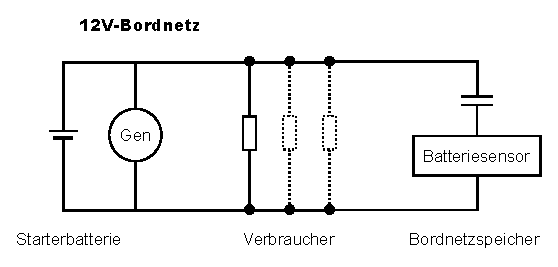
\includegraphics[width=0.7\textwidth]{images/inkscape/circuits/12V_Bordnetz}
	\caption{Prinzipschaltbild des bereits etablierten 12V-Bordnetzes}
	\label{fig:12V_Bordnetz}
\end{figure}

\begin{figure}[htbp]
	\centering
	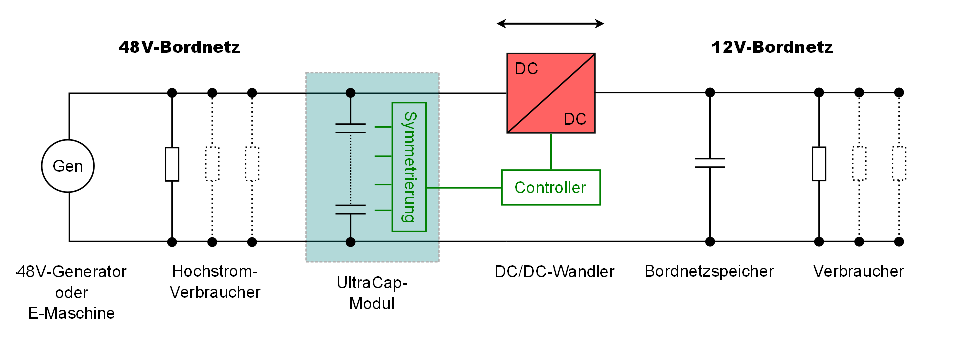
\includegraphics[width=1.0\textwidth]{images/inkscape/circuits/48V_12V_Bordnetz}
	\caption{Prinzipschaltbild des zukünftigen 48V/12V-Bordnetzes mit UltraCap-Modul und DC/DC-Wandler}
	\label{fig:48V_12V_Bordnetz}
\end{figure}

\subsection{Inkscape document with pdf-tex}
Just save the inkscape document as pdf and choose the option \emph{PDF+LaTeX: Text in PDF weglassen und LaTeX Datei erstellen}.

\begin{figure}[ht]
	\begin{center}
		\def\svgwidth{\linewidth}\small
		\import{./images/inkscape/charts/}{flowchart.pdf_tex}
		\caption{Overview of work packages and assignments}
		\label{fig:assignment_wp}
	\end{center}
\end{figure}

\begin{figure}[ht]
	\centering
	\def\svgwidth{\linewidth}\footnotesize
	\import{./images/inkscape/charts/}{gantt_chart.pdf_tex}
	\caption{Gantt chart of the proposed work program}
	\label{fig:Gantt}
\end{figure}

%===================================================
\section{Blockschaltbilder}
You can draw block diagrams with Tikz. For this, you can use the commands defined in the TeX-File \emph{blockschaltbilder} (setup/blockschaltbilder). Some examples follow now: see Fig.~\ref{fig:zwei-freiheitsgrade-regelung}, Fig,~\ref{fig:zwei-freiheitsgrade-regelung-zustand}.

\begin{figure}[tp]
	\centering
	\scalebox{0.95}{
		\begin{tikzpicture}

  % Knoten / Blöcke
  \coordinate (sollwert) at (-4.0, 0);
  \coordinate (ausgang) at (4.0, 0);
  \Summationsstelle{summation}{0, 0}{0.4 cm}
  \Summationsstelle{soll-ist}{0, -3}{0.4 cm}
  \UeFunk{strecke}{2, 0}{1.0 cm}{$G(s)$}
  \UeFunk{regler}{0, -1.5}{1.0 cm}{$R(s)$}
  \UeFunk{vorsteuerung}{-2, 0}{1.0 cm}{$G_{\mathrm{V}}(s)$}
  \Verzweigung{verzw-ausgang}{3.20, 0}{2 pt}
  \Verzweigung{verzw-sollwert}{-3.20, 0}{2 pt}

  % Signalflüsse
  \draw[thick, -latex'] (summation)      -- (strecke);
  \draw[thick, -latex'] (regler)         -- (summation);
  \draw[thick, -latex'] (vorsteuerung)   -- (summation);
  \draw[thick, -latex'] (soll-ist)       -- (regler);
  \draw[thick         ] (strecke)        -- (verzw-ausgang);
  \draw[thick, -latex'] (verzw-ausgang)  -- (ausgang);
  \draw[thick, -latex'] (verzw-ausgang)  |- (soll-ist);
  \draw[thick         ] (sollwert)       -- (verzw-sollwert);
  \draw[thick, -latex'] (verzw-sollwert) -- (vorsteuerung);
  \draw[thick, -latex'] (verzw-sollwert) |- (soll-ist);

  % Beschriftungen
  \node[outer sep = 0.1 cm, above right] at (sollwert) {$w$};
  \node[outer sep = 0.1 cm, above left ] at (strecke.west) {$u$};
  \node[outer sep = 0.1 cm, above left ] at (ausgang) {$y$};
  \node[outer sep = 0.1 cm, below left ] at (regler.south) {$e$};
  \node[                    above right] at (soll-ist.east) {$-$};

\end{tikzpicture}
}
	\caption{Something interesting.}
	\label{fig:zwei-freiheitsgrade-regelung}
\end{figure}

\begin{figure}[tp]
	\centering
	\scalebox{0.95}{
		\begin{tikzpicture}

  % Knoten / Blöcke
  \coordinate (sollwert) at (-4.0, 0);
  \coordinate (ausgang) at (5.5, 0);
  \Summationsstelle{summation}{0, 0}{0.4 cm}
  \Summationsstelle{soll-ist}{0, -3}{0.4 cm}
  \UeFunk[align = left, inner sep = 8 pt]{strecke}{2.5, 0}{1.0 cm}{ %
    $\dot{\bm{x}} = \bm{A}\mathbf{x} + \bm{b} u$ \\[8 pt] %
    $y = \bm{c}^\mathrm{T} \bm{x}$ %
  }
  \UeFunk{regler}{0, -1.5}{1.0 cm}{$\bm{r}^\mathrm{T}$}
  \UeFunk{vorsteuerung}{-2, 0}{1.0 cm}{$m_u$}
  \UeFunk{vorsteuerung-zustand}{-2, -3}{1.0 cm}{$\bm{m}_{\bm{x}}$}
  \Verzweigung{verzw-sollwert}{-3.20, 0}{2 pt}

  % Signalflüsse
  \draw[thick,       -latex'] (summation)            -- (strecke);
  \draw[thick,       -latex'] (regler)               -- (summation);
  \draw[thick,       -latex'] (vorsteuerung)         -- (summation);
  \draw[ultra thick, -latex'] (soll-ist)             -- (regler);
  \draw[thick,       -latex'] (strecke)              -- (ausgang);
  \draw[ultra thick, -latex'] (strecke)              |- (soll-ist);
  \draw[thick               ] (sollwert)             -- (verzw-sollwert);
  \draw[thick,       -latex'] (verzw-sollwert)       |- (vorsteuerung-zustand);
  \draw[thick,       -latex'] (verzw-sollwert)       |- (vorsteuerung);
  \draw[ultra thick, -latex'] (vorsteuerung-zustand) -- (soll-ist);

  % Beschriftungen
  \node[outer sep = 0.1 cm, above right] at (sollwert) {$w$};
  \node[outer sep = 0.1 cm, above left ] at (strecke.west) {$u$};
  \node[outer sep = 0.1 cm, above left ] at (ausgang) {$y$};
  \node[outer sep = 0.1 cm, below left ] at (regler.south) {$\bm{e}$};
  \node[                    above right] at (soll-ist.east) {$-$};
  \node[outer sep = 0.1 cm, below left ] at (soll-ist.west) {$\bm{x_{\mathrm{soll}}}$};
  \node[outer sep = 0.1 cm, below right] at (soll-ist.east) {$\bm{x}$};

\end{tikzpicture}
}
	\caption{Something interesting.}
	\label{fig:zwei-freiheitsgrade-regelung-zustand}
\end{figure}

	

%===================================================
\section{ToDo Notes}
%\tikzexternaldisable
\todoX{Chapter Layout}
\todoX{derive bounds for arm7}
\todoX{pseudo code for RRT*-GBO}
\todoX{pseudo code for MC}
\todoX{pseudo code for PHO}
\todoX{pseudo code for IPSO}
\todoX{iterative violation detector/via point cluster insertion}
\todoX{Analytical Proof of optimal result for unconstrained SO3 maneuver}
\todoX{Verification of SO3 result with 1 EZ (trajectory tangeant to the EZ)}
\todoX{Kinematics/dynamics of SO3}
\todoX{Kinematics/dynamics of Arm7}

\todoY{ example of blue todo}
\todoZ{ example of green todo}

\listoftodos
%\tikzexternalenable


%===================================================
\section{Tables}
\LaTeX{} tables are (almost) trivial! Cf.\ \cref{tab:example}. But do not \textit{verkünstel} yourself. We recommend to use the booktabs package or at least to adhere to their proposed table style when ever the scope of the table allows for it. ( \url{https://ctan.mirror.norbert-ruehl.de/macros/latex/contrib/booktabs/booktabs.pdf})

\begin{table}
  \centering
  \caption{Funny webcomics}
  \label{tab:example}
  \begin{tabular}{llll}
    \toprule
    Title                    & Author     & Date         & Link                                                    \\
    \midrule
    Highway Engineer Pranks  & R.\ Munroe & 2007-04-25   & \href{http://xkcd.com/253/}{xkcd.com}                   \\
    Stop Being Engineers!    & S.\ Adams  & 2014-02-02   & \href{http://dilbert.com/strip/2014-02-02}{dilbert.com} \\
    The Typographical Terror & D.\ Malki  & 2010--08--20 & \href{http://wondermark.com/650/}{wondermark.com}       \\
    \bottomrule
  \end{tabular}
\end{table}


\section{Listings}
Quine in \cref{lst:quine:c} was found \href{https://www.nyx.net/~gthompso/self_c.txt}{here} (search for Jeff Hollingsworth's quine),
quine in \cref{lst:quine:matlab} \href{http://blog.garritys.org/2009/10/quines.html}{here}. The code in
\cref{lst:sierpinski} was found \href{http://rosettacode.org/wiki/Sierpinski_carpet#Python}{here}.

\begin{lstlisting}[language = C, label = lst:quine:c, caption = {An elegant C quine}]
#define Z(q)q,#q
main()printf(Z("#define Z(q)q,#q\nmain()printf(Z(%s));\n"));
\end{lstlisting}

\begin{lstlisting}[label = lst:quine:matlab, caption = {An elegant MATLAB quine}]
a=['ns}z2e1kGe1116k6111gE16;:6ek7;:61gg3E1'];
disp(['a=[''',a,'''];',10,[a-10,']]);']]);
\end{lstlisting}

\lstinputlisting[language = Python, label = lst:sierpinski, caption = {Sierpinski carpet in Python}]{./sources/sierpinski.py}


\section{Language support}
This template is configured for English throughout. The document class and all generated
front matter use English as the only document language.


\section{Abbreviations and acronyms}
Abbreviations and acronyms are defined in \verb|auxfiles/abbreviationsAndAcronyms.tex|.
You can typeset them using the \verb|\ac{}| command. Refer to \texttt{acro} package
documentation for specialized commands (\verb|\acs{}|, \verb|\acl{}|, \verb|\acp{}|,
\verb|\iac{}|, \verb|\Iac{}|, \ldots).

Usage example:
\begin{itemize}
  \item An abbreviation is explained if used for the first time: \ac{MPC};
  \item subsequently, only the short version is used: \ac{MPC};
  \item however, you can force \texttt{acro} to use the long version anytime: \acl{MPC}.
\end{itemize}

\emph{Important:} If you want to have only the actually used abbreviations and acronyms
in the list (\cref{sc:abbreviationsAndAcronyms}), edit \verb|setup/settings.tex|: Find
the \verb|\acsetup{}| command and set \verb|list/display| to \texttt{used}.


\section{References}
\subsection{Hyperlinks}
See \url{https://en.wikibooks.org/wiki/LaTeX/Hyperlinks}.

Also, always use \verb|\cref{}| for referencing equations, tables or other things!

\subsection{Literature}
Cite multiple references:
\textcite{Bronstein2012,Follinger2013,Gamma2004,Gantmacher2000a,Gantmacher2000b,%
  Golub2013,Horn2013,LaSalle1961,Mehlhorn2008,Sontag1998,Adamy2009,Horn1994,Watkins2002}.

If you want to have only the reference number:
\cite{Bronstein2012,Follinger2013,Gamma2004,Gantmacher2000a,Gantmacher2000b,Golub2013,%
  Horn2013,LaSalle1961,Mehlhorn2008,Sontag1998,Adamy2009,Horn1994,Watkins2002}.

If you want to reference a specific section: \cite[\S~5.2.2, pp.~248--250]{Golub2013}.

If you want to reference a specific equation: \cite[Eq.~(13.22), p.~721]{Bronstein2012}.
